%%%%%%%%%% !TEX program = pdflatex %%%%%%%%%%
% !TEX program = pdflatex
% !Mode:: "TeX:UTF-8"
% \def\usewhat{dvipdfmx}                              % 定义编译方式 dvipdfmx 或者 pdflatex ,默认为 dvipdfmx
													% 方式编译,如果需要修改,只需改变花括号中的内容即可。
%\setlength{\baselineskip}{20pt}
%\setlength{\headheight}{25pt}
\documentclass[a4paper,12.5pt,openany,twoside,openright]{book}

                                           % 如果论文超过60页 可以使用twoside 双面打印
% !TEX program = pdflatex
% !Mode:: "TeX:UTF-8"
%  Authors: 杜家宜   Jiayi Du: Max_dujiayi@gmail.com     湖南大学2010级计算机科学与技术专业博士生

%%%%%%%%%% Package %%%%%%%%%%%%
\usepackage[chapter]{algorithm}
\usepackage{pdfpages}% 方便插入签字版权页
\usepackage{algorithmic}
\usepackage{graphicx}                       % 支持插图处理
\usepackage{geometry}
\geometry{left=2.5cm,right=2.5cm,top=2cm,bottom=2.5cm,footskip=1.1cm,headsep=0.7cm,head=0.4cm}
% 支持版面尺寸设置
\usepackage{titlesec}                       % 控制标题的宏包
\usepackage{titletoc}                       % 控制目录的宏包
\usepackage{fancyhdr}                       % fancyhdr宏包 支持页眉和页脚的相关定义
\usepackage[UTF8]{ctex}                    % 支持中文显示
\usepackage{cite}
\usepackage{color}                          % 支持彩色
\usepackage{amsmath}                        % AMSLaTeX宏包 用来排出更加漂亮的公式
\usepackage{amssymb}                        % 数学符号生成命令
\usepackage{mathrsfs}                       % Add by Lijianmin
\usepackage{cases}
\usepackage[below]{placeins}                %允许上一个section的浮动图形出现在下一个section的开始部分,还提供\FloatBarrier命令,使所有未处理的浮动图形立即被处理
\usepackage{flafter}                        % 使得所有浮动体不能被放置在其浮动环境之前,以免浮动体在引述它的文本之前出现.
\usepackage{multirow}                       % 使用Multirow宏包,使得表格可以合并多个row格
\usepackage{booktabs}                       % 表格,横的粗线;\specialrule{1pt}{0pt}{0pt}
\usepackage{longtable}                      % 支持跨页的表格。
\usepackage{tabularx}                       % 自动设置表格的列宽
\usepackage{setspace}
\usepackage{subfigure}                      % 支持子图 %centerlast 设置最后一行是否居中
\usepackage[subfigure]{ccaption}            % 支持子图的中文标题
\usepackage[sort&compress,numbers]{natbib}  % 支持引用缩写的宏包
\usepackage{enumitem}                       % 使用enumitem宏包,改变列表项的格式
\usepackage{calc}                           % 长度可以用+ - * / 进行计算
\usepackage{txfonts}                        % 字体宏包
\usepackage{bm}                             % 处理数学公式中的黑斜体的宏包
\usepackage[amsmath,thmmarks,hyperref]{ntheorem}  % 定理类环境宏包,其中 amsmath 选项用来兼容 AMS LaTeX 的宏包
\usepackage{CJKnumb}                        % 提供将阿拉伯数字转换成中文数字的命令
\usepackage{indentfirst}                    % 首行缩进宏包
\usepackage{CJKutf8}                        % 用在UTF8编码环境下,它可以自动调用CJK,同时针对UTF8编码作了设置。
\usepackage{CJK}
\usepackage{fancyhdr}
\usepackage{lastpage}
\usepackage{layout}
\usepackage[titles,subfigure]{tocloft}      %控制生成的表格和图片的目录格式
%\usepackage{caption}
% Add by Lijianmin
%\usepackage{hypbmsec}                      % 用来控制书签中标题显示内容
%\usepackage{bbding}
%如果您的pdf制作中文书签有乱码使用如下命令,就可以解决了
%Modified by Lijianmin
\usepackage[unicode,               % pdflatex, pdftex 这里决定运行文件的方式不同
%\usepackage[dvipdfm, unicode,               % pdflatex, pdftex 这里决定运行文件的方式不同
pdfstartview=FitH,
%CJKbookmarks=true,
bookmarksnumbered=true,
bookmarksopen=true,
colorlinks=true,
pdfborder={0 0 1},
citecolor=black,
linkcolor=black,
anchorcolor=black,
urlcolor=black,
breaklinks=true
]{hyperref}

\usepackage{upgreek} % 直体希腊字母,如,微米 $\upmu$m,用在正文里的单位
\usepackage{diagbox} % 表格里面使用斜角
\usepackage{float} % 强制使图片放置在当前位置,\begin{figure}[H]...\end{figure},关键在H
\usepackage{hyperref}
\usepackage{bookmark}
\usepackage{tocloft} % 控制目录,索引格式,非常好用
%\usepackage[BoldFont]{xeCJK}
\usepackage{enumitem}                      % 定义本文所使用宏包
\graphicspath{{figures/}}                  % 定义所有的.eps文件在figures子目录下
\begin{document}                           % 开始全文
\begin{CJK*}{UTF8}{song}                   % 开始中文字体使用
% !Mode:: "TeX:UTF-8"
%  Authors: 杜家宜   Jiayi Du: Max_dujiayi@gmail.com     湖南大学2010级计算机科学与技术专业博士生

%%%%%%%%%% Fonts Definition and Basics %%%%%%%%%%%%%%%%%
\newcommand{\song}{\CJKfamily{song}}    % 宋体
\newcommand{\fs}{\CJKfamily{fs}}        % 仿宋体
\newcommand{\kai}{\CJKfamily{kai}}      % 楷体
\newcommand{\hei}{\CJKfamily{hei}}      % 黑体
\newcommand{\li}{\CJKfamily{li}}        % 隶书
\newcommand{\yihao}{\fontsize{26pt}{26pt}\selectfont}       % 一号, 1.倍行距
\newcommand{\xiaoyi}{\fontsize{24pt}{24pt}\selectfont}      % 小一, 1.倍行距
\newcommand{\erhao}{\fontsize{22pt}{22pt}\selectfont}       % 二号, 1.倍行距
\newcommand{\xiaoer}{\fontsize{18pt}{18pt}\selectfont}      % 小二, 单倍行距
\newcommand{\sanhao}{\fontsize{16pt}{16pt}\selectfont}      % 三号, 1.倍行距
\newcommand{\xiaosan}{\fontsize{15pt}{15pt}\selectfont}     % 小三, 1.倍行距
\newcommand{\sihao}{\fontsize{14pt}{14pt}\selectfont}       % 四号, 1.0倍行距
\newcommand{\xiaosi}{\fontsize{12.5pt}{12.5pt}\selectfont}  % 小四, 1.倍行距
\newcommand{\wuhao}{\fontsize{10.5pt}{10.5pt}\selectfont}   % 五号, 单倍行距
\newcommand{\tuzhu}{\fontsize{10.5pt}{15.5pt}\selectfont}   % 五号, 单倍行距
\newcommand{\xiaowu}{\fontsize{9pt}{9pt}\selectfont}        % 小五, 单倍行距
\setlength{\headheight}{20pt}
%\CJKcaption{gb_452}
\CJKtilde  % 重新定义了波浪符~的意义
\newcommand\prechaptername{第~}
\newcommand\postchaptername{~章}

% 调整罗列环境的布局 % Modified by Li Jianmin
\setitemize{leftmargin=0em,itemindent=3em,itemsep=0em,partopsep=0em,parsep=0em,topsep=-0em}
\setenumerate{leftmargin=0em,itemindent=3em,itemsep=0em,partopsep=0em,parsep=0em,topsep=0em}


%避免宏包 hyperref 和 arydshln 不兼容带来的目录链接失效的问题。
\def\temp{\relax}
\let\temp\addcontentsline
\gdef\addcontentsline{\phantomsection\temp}

% 自定义项目列表标签及格式 \begin{publist} 列表项 \end{publist}
\newcounter{pubctr} % 自定义新计数器
\newenvironment{publist}{%%%%% 定义新环境
\begin{list}{[\arabic{pubctr}]} %% 标签格式
    {
     \usecounter{pubctr}
     \setlength{\leftmargin}{2em}     % 左边界 \leftmargin =\itemindent + \labelwidth + \labelsep
     \setlength{\itemindent}{0em}     % 标号缩进量
     \setlength{\labelsep}{1em}       % 标号和列表项之间的距离,默认0.5em
     \setlength{\rightmargin}{0em}    % 右边界
     \setlength{\topsep}{0ex}         % 列表到上下文的垂直距离
     \setlength{\parsep}{0ex}         % 段落间距
     \setlength{\itemsep}{0ex}        % 标签间距
     \setlength{\listparindent}{0pt} % 段落缩进量
    }}
{\end{list}}%%%%%


\makeatletter
\renewcommand\normalsize{
  \@setfontsize\normalsize{12.5pt}{12.5pt} % 小四对应12pt
  \setlength\abovedisplayskip{4pt}
  \setlength\abovedisplayshortskip{4pt}
  \setlength\belowdisplayskip{\abovedisplayskip}
  \setlength\belowdisplayshortskip{\abovedisplayshortskip}
    \let\@listi\@listI}
\def\defaultfont{\renewcommand{\baselinestretch}{1.65}\normalsize\selectfont}


% 设置行距和段落间垂直距离

\setlength{\baselineskip}{20pt}
\renewcommand{\CJKglue}{\hskip 0.5pt plus \baselineskip} %加大字间距,使每行35个字


\makeatother

%%%%%%%%%%%%% Contents %%%%%%%%%%%%%%%%%
\renewcommand{\contentsname}{目\quad录}
\setcounter{tocdepth}{2}
\renewcommand{\cftchapdotsep}{1}
\renewcommand{\cftsecdotsep}{1}
\renewcommand\cftbeforechapskip{0.1em}
\renewcommand{\cftchapfont}{\hei\xiaosi}
\renewcommand\cftchappresnum{第~}
\renewcommand\cftchapaftersnum{~章}
\renewcommand\cftchapnumwidth{4em}
\renewcommand{\cftchappagefont}{\song\xiaosi}
\renewcommand{\cftsecfont}{\song\xiaosi}
\renewcommand{\cftsecpagefont}{\song\xiaosi}
\renewcommand{\cftsubsecfont}{\song\xiaosi}
\renewcommand{\cftsubsecpagefont}{\song\xiaosi}
%\renewcommand{\cftsubsubsecfont}{\song\xiaosi}
%\renewcommand{\cftsubsubsecpagefont}{\song\xiaosi}
%\titlecontents{chapter}[0em]{\xiaosi\hei}%
%             {\prechaptername~~\thecontentslabel~~\postchaptername~~~}{} %
%             {\titlerule*[5pt]{$\cdot$}\xiaosi\contentspage}
%\titlecontents{section}[2.5em]{\xiaosi\song} %
%            {\thecontentslabel\quad}{} %
%            {\hspace{.25em}\titlerule*[5pt]{$\cdot$}\xiaosi\contentspage}
%\titlecontents{subsection}[3.25em]{\xiaosi\song} %
%            {\thecontentslabel\quad}{} %
%            {\hspace{.25em}\titlerule*[5pt]{$\cdot$}\xiaosi\contentspage}
%\titlecontents{subsubsection}[4em]{\xiaosi\song} %
%			{\thecontentslabel\quad}{} %
%			{\hspace{.25em}\titlerule*[5pt]{$\cdot$}\xiaosi\contentspage}
\renewcommand{\cftdotsep}{1.1}
\renewcommand{\listfigurename}{插图索引}
\setcounter{lofdepth}{1}
\renewcommand{\cftfigpresnum}{图~}
\setlength{\cftfignumwidth}{4.5em}
%\titlefigures{chapter}[1em]{\xiaosi\hei}%
%             {\prechaptername~~\thecontentslabel~~\postchaptername~~~}{} %
%            {\titlerule*[5pt]{$\cdot$}\xiaosi\contentspage}
\renewcommand{\listtablename}{附表索引}
\renewcommand{\cfttabpresnum}{表~}
\setlength{\cfttabnumwidth}{4em}

%%删除表格和插图因章不同中的空行%%%
\makeatletter
\def\@chapter[#1]#2{\ifnum \c@secnumdepth >\m@ne
                       \if@mainmatter
                         \refstepcounter{chapter}%
                         \typeout{\@chapapp\space\thechapter.}%
                         \addcontentsline{toc}{chapter}%
                                   {\protect\numberline{\thechapter}#1}%
                       \else
                         \addcontentsline{toc}{chapter}{#1}%
                       \fi
                    \else
                      \addcontentsline{toc}{chapter}{#1}%
                    \fi
                    \chaptermark{#1}%
                    \if@twocolumn
                      \@topnewpage[\@makechapterhead{#2}]%
                    \else
                      \@makechapterhead{#2}%
                      \@afterheading
                    \fi}
\makeatother


%%%%%%%%%% Chapter and Section %%%%%%%%%%%%%%%%%
\setcounter{secnumdepth}{4}
\setlength{\parindent}{2em}
\renewcommand{\chaptername}{\prechaptername\arabic{chapter}\postchaptername}
\titleformat{\chapter}{\centering\xiaoer\hei}{\chaptername}{1em}{}
\titlespacing{\chapter}{0pt}{0pt}{18pt}
\titleformat{\section}{\xiaosan\hei}{\thesection}{1em}{}
\titlespacing{\section}{0pt}{12pt}{12pt}
\titleformat{\subsection}{\sihao\hei}{\thesubsection}{0.5em}{}
\titlespacing{\subsection}{0pt}{6pt}{6pt}
\titleformat{\subsubsection}{\xiaosi\hei}{\thesubsubsection}{0.5em}{}
\titlespacing{\subsubsection}{0pt}{6pt}{6pt}

%%%%%%%%%% Table, Figure and Equation %%%%%%%%%%%%%%%%%
\renewcommand{\tablename}{表} % 插表题头
\renewcommand{\figurename}{图} % 插图题头
\renewcommand{\thefigure}{\arabic{chapter}.\arabic{figure}} % 使图编号为 7.1 的格式 %\protect{~}
\renewcommand{\thetable}{\arabic{chapter}.\arabic{table}}%使表编号为 7.1 的格式
\renewcommand{\theequation}{\arabic{chapter}.\arabic{equation}}%使公式编号为 7.1 的格式
\renewcommand{\thesubfigure}{\alph{subfigure})}%使子图编号为a)的格式
\renewcommand{\thesubtable}{(\alph{subtable})} %使子表编号为a)的格式
\makeatletter
\renewcommand{\p@subfigure}{\thefigure~} %使子图引用为 7.1 a) 的格式,母图编号和子图编号之间用~ 加一个空格
\makeatother


%% 定制浮动图形和表格标题样式
\makeatletter
\long\def\@makecaption#1#2{%
   \vskip\abovecaptionskip
   \sbox\@tempboxa{\centering\wuhao\hei{#1~~#2} }%
   \ifdim \wd\@tempboxa >\hsize
     \centering\wuhao\hei{#1~~#2} \par
   \else
     \global \@minipagefalse
     \hb@xt@\hsize{\hfil\box\@tempboxa\hfil}%
   \fi
   \vskip\belowcaptionskip}
\makeatother
\captiondelim{~~~~} %用来控制longtable表头分隔符

%%%%%%%%%% Theorem Environment %%%%%%%%%%%%%%%%%
\theoremstyle{plain}
\theorembodyfont{\xiaosi\song}%\rmfamily}
\theoremheaderfont{\xiaosi\hei}%\rmfamily}
\setlength{\theorempreskipamount}{0em} %调整定理环境与上文的距离
\setlength{\theorempostskipamount}{0em} %调整定理环境与下文的距离
\newtheorem{theorem}{定理~}[chapter]
\newtheorem{lemma}{引理~}[chapter]
\newtheorem{axiom}{公理~}[chapter]
\newtheorem{proposition}{命题~}[chapter]
\newtheorem{corollary}{推论~}[chapter]
\newtheorem{definition}{\hskip 2em 定义~}[chapter]
\newtheorem{conjecture}{猜想~}[chapter]
\newtheorem{example}{例~}[chapter]
\newtheorem{remark}{注~}[chapter]
\floatname{algorithm}{算法}% 将英文的algorithm改为算法
\renewcommand{\algorithmicrequire}{\textbf{Input:}}
\renewcommand{\algorithmicensure}{\textbf{Output:}}
\newcommand{\tabincell}[2]{\begin{tabular}{@{}#1@{}}#2\end{tabular}}%表格合并
\newenvironment{proof}{\noindent{\hei 证明:}}{\hfill $ \square $ \vskip 4mm}
\theoremsymbol{$\square$}

%%%%%%%%%% Page: number, header and footer  页码%%%%%%%%%%%%%%%%%

%\frontmatter 或 \pagenumbering{roman}
%\mainmatter 或 \pagenumbering{arabic}
\makeatletter
\renewcommand\frontmatter{\clearpage
  \@mainmatterfalse
  \pagenumbering{Roman}} % 正文前罗马字体编号
\makeatother


%%%%%%%%%% References %%%%%%%%%%%%%%%%%
\renewcommand{\bibname}{参考文献}
% 重定义参考文献样式,来自thu
\makeatletter
\renewenvironment{thebibliography}[1]{%
   \chapter*{\bibname}%
   \xiaosi
   \list{\@biblabel{\@arabic\c@enumiv}}%
        {\renewcommand{\makelabel}[1]{##1\hfill}
         \setlength{\baselineskip}{21pt}
         \settowidth\labelwidth{0.5cm}
         \setlength{\labelsep}{0pt}
         \setlength{\itemindent}{0pt}
         \setlength{\leftmargin}{\labelwidth+\labelsep}
         \addtolength{\itemsep}{-0.7em}
         \usecounter{enumiv}%
         \let\p@enumiv\@empty
         \renewcommand\theenumiv{\@arabic\c@enumiv}}%
    \sloppy\frenchspacing
    \clubpenalty4000%
    \@clubpenalty \clubpenalty
    \widowpenalty4000%
    \interlinepenalty4000%
    \sfcode`\.\@m}
   {\def\@noitemerr
     {\@latex@warning{Empty `thebibliography' environment}}%
    \endlist\frenchspacing}
\makeatother

\addtolength{\bibsep}{5pt} % 增加参考文献间的垂直间距
\setlength{\bibhang}{2em} %每个条目自第二行起缩进的距离

% 参考文献引用作为上标出现
\newcommand{\mycite}[1]{\scalebox{1.3}[1.3]{\raisebox{-0.65ex}{\cite{#1}}}}
%\newcommand{\citenormal}[1]{\cite{#1}}
%\makeatletter
%   \def\@cite#1#2{\textsuperscript{[{#1\if@tempswa , #2\fi}]}}
%\makeatother

%% 引用格式
\bibpunct{[}{]}{,}{s}{}{,}

%%%%%%%%%% Cover %%%%%%%%%%%%%%%%%
% 封面、摘要、版权、致谢格式定义
\makeatletter

\def\dtitle#1{\def\@dtitle{#1}}\def\@dtitle{}
\def\ctitle#1{\def\@ctitle{#1}}\def\@ctitle{}
\def\etitle#1{\def\@etitle{#1}}\def\@etitle{}
\def\caffil#1{\def\@caffil{#1}}\def\@caffil{}
\def\cmacrosubject#1{\def\@cmacrosubject{#1}}\def\@cmacrosubject{}
\def\cmacrosubjecttitle#1{\def\@cmacrosubjecttitle{#1}}\def\@cmacrosubjecttitle{}
\def\csubject#1{\def\@csubject{#1}}\def\@csubject{}
\def\csubjecttitle#1{\def\@csubjecttitle{#1}}\def\@csubjecttitle{}
\def\cmajor#1{\def\@cmajor{#1}}\def\@cmajor{}
\def\cauthor#1{\def\@cauthor{#1}}\def\@cauthor{}
\def\cauthortitle#1{\def\@cauthortitle{#1}}\def\@cauthortitle{}
\def\csupervisor#1{\def\@csupervisor{#1}}\def\@csupervisor{}
\def\csupervisortitle#1{\def\@csupervisortitle{#1}}\def\@csupervisortitle{}
\def\cdate#1{\def\@cdate{#1}}\def\@cdate{}
\def\untitle#1{\def\@untitle{#1}}\def\@untitle{}
\def\declaretitle#1{\def\@declaretitle{#1}}\def\@declaretitle{}
\def\declarecontent#1{\def\@declarecontent{#1}}\def\@declarecontent{}
\def\authorizationtitle#1{\def\@authorizationtitle{#1}}\def\@authorizationtitle{}
\def\authorizationcontent#1{\def\@authorizationcontent{#1}}\def\@authorizationconent{}
\def\authorizationadd#1{\def\@authorizationadd{#1}}\def\@authorizationadd{}
\def\authorsigncap#1{\def\@authorsigncap{#1}}\def\@authorsigncap{}
\def\supervisorsigncap#1{\def\@supervisorsigncap{#1}}\def\@supervisorsigncap{}
\def\signdatecap#1{\def\@signdatecap{#1}}\def\@signdatecap{}
\long\def\cabstract#1{\long\def\@cabstract{#1}}\long\def\@cabstract{}
\long\def\eabstract#1{\long\def\@eabstract{#1}}\long\def\@eabstract{}
\def\ckeywords#1{\def\@ckeywords{#1}}\def\@ckeywords{}
\def\ekeywords#1{\def\@ekeywords{#1}}\def\@ekeywords{}
\def\cheading#1{\def\@cheading{#1}}\def\@cheading{}
\def\cnumber#1{\def\@cnumber{#1}}\def\@cnumber{}
\def\csecret#1{\def\@csecret{#1}}\def\@csecret{}
\def\chnunumer#1{\def\@chnunumer{#1}}\def\@chnunumer{}
\def\cclassnumber#1{\def\@cclassnumber{#1}}\def\@cclassnumber{}
\def\chnuname#1{\def\@chnuname{#1}}\def\@chnuname{}
\def\cchair#1{\def\@cchair{#1}}\def\@cchair{}
\def\ddate#1{\def\@ddate{#1}}\def\@ddate{}
%英文内封
\def\ename#1{\def\@ename{#1}}\def\@ename{}
\def\cbe#1{\def\@cbe{#1}}\def\@cbe{}
\def\cms#1{\def\@cms{#1}}\def\@cms{}
\def\cdegree#1{\def\@cdegree{#1}}\def\@cdegree{}
\def\cclass#1{\def\@cclass{#1}}\def\@cclass{}
\def\emajor#1{\def\@emajor{#1}}\def\@emajor{}
\def\ehnu#1{\def\@ehnu{#1}}\def\@ehnu{}
\def\esupervisor#1{\def\@esupervisor{#1}}\def\@esupervisor{}
\def\edate#1{\def\@edate{#1}}\def\@edate{}
\def\elevel#1{\def\@elevel{#1}}\def\@elevel{}



\newlength{\@title@width}
\def\@put@covertitle#1{\makebox[\@title@width][s]{#1}}
% 定义封面
\def\makecover{
%\cleardoublepage%
   \phantomsection
    \pdfbookmark[-1]{\@ctitle}{ctitle}

    \begin{titlepage}
    \begin{center}

      \setlength{\@title@width}{3.5cm}
       {
  \begin{tabular}{lcclc}
   \xiaosi\hei{学校代号}&  \underline{\makebox[\@title@width][c]{\@chnunumer}}&\qquad \qquad \qquad \qquad \qquad & \xiaosi\hei{学\qquad 号}&  \underline{\makebox[\@title@width][c]{\@cnumber}}\\
   \xiaosi\hei{分~~类~~~号}&  \underline{\makebox[\@title@width][c]{\@cclassnumber}}&\qquad \qquad \qquad \qquad \qquad & \xiaosi\hei{密\qquad 级}&  \underline{\makebox[\@title@width][c]{\@csecret}} \\
   \end{tabular}
   }

 \begin{figure}[h]
  \centering
  
\includegraphics[width=0.3\textwidth]{figures/Hnulogo}
  \end{figure}
      \vspace*{1cm}
      {\hei\erhao \@cheading}

      \vspace*{1cm}


      \begin{center}
      \begin{spacing}{1.5}
      %\hei\yihao \@dtitle%原标题断字会影响页眉
      \hei\yihao \@ctitle%标题可以使用断字
      \end{spacing}
      \end{center}
%\makebox[宽度][位置]{文本}中可指定盒子宽度,文本在盒子中的位置(l:左端;r:右端;s:两端,默认是居中)
      \vspace{\baselineskip}
      \setlength{\@title@width}{8.5cm}
  {
\begin{spacing}{2.1}
	\makebox[3.3cm][s]{\xiaosi\hei{学位申请人姓名}}\xiaosi\song\underline{\makebox[\@title@width][l]{\qquad\@cauthor}} \\
	\makebox[3.3cm][s]{\xiaosi\hei{培~~~~养~~~~单~~~~位}} \xiaosi\song\underline{\makebox[\@title@width][l]{\qquad\@caffil}} \\
	\makebox[3.3cm][s]{\xiaosi\hei{导师姓名及职称}} \xiaosi\song\underline{\makebox[\@title@width][l]{\qquad\@csupervisor}} \\
	\makebox[3.3cm][s]{\xiaosi\hei{学~~~~科~~~~专~~~~业}} \xiaosi\song\underline{\makebox[\@title@width][l]{\qquad\@csubject}} \\
	\makebox[3.3cm][s]{\xiaosi\hei{研~~~~究~~~~方~~~~向}} \xiaosi\song\underline{\makebox[\@title@width][l]{\qquad\@cmajor}}\\
	\makebox[3.3cm][s]{\xiaosi\hei{论~文~提~交~日~~期}} \xiaosi\song\underline{\makebox[\@title@width][l]{\qquad\@cdate}} \\
\end{spacing}
 }
 \end{center}


\clearpage
\thispagestyle{empty} %去掉页眉页脚

\noindent
\makebox[2.59cm][s]{}{\begin{tabular}{ll}
\makebox[2cm][s]{\xiaosi\hei 学校代号:}\xiaosi\song~~\@chnunumer \\
\makebox[2cm][s]{\xiaosi\hei 学\qquad~号:}\xiaosi\song~~\@cnumber\\
\makebox[2cm][s]{\xiaosi\hei 密\qquad~级:}\xiaosi\song~~\@csecret\\
\end{tabular}
}

%
\vspace{5\baselineskip}

\noindent
\makebox[2.59cm][s]{}{
\xiaoer\song \@chnuname \@cheading
}
\\
\vspace{4\baselineskip}

\begin{spacing}{2}
\hangafter=1\hangindent=2.7cm   %换行后自动缩进
{\noindent
\makebox[2.59cm][s]{} {\hei\erhao\@ctitle}}%{\hei\erhao\@ctitle}}
\end{spacing}
\vspace{4\baselineskip}

\setlength{\@title@width}{6.5cm}
  {
  \begin{spacing}{2}
  \xiaosi
  \noindent
  \makebox[2.59cm][s]{}{
    \begin{tabular}{lc}
   \underline{\makebox[3.3cm][s]{\xiaosi\hei学位申请人姓名:}\song\makebox[\@title@width][l]{\qquad\qquad\@cauthor}} \\
   \underline{\makebox[3.3cm][s]{\xiaosi\hei导师姓名及职称:}\song\makebox[\@title@width][l]{\qquad\qquad\@csupervisor}} \\
   \underline{\makebox[3.3cm][s]{\xiaosi\hei培~~~~养~~~~单~~~~位:}\song\makebox[\@title@width][l]{\qquad\qquad\@caffil}} \\
   \underline{\makebox[3.3cm][s]{\xiaosi\hei专~~~~业~~~~名~~~~称:}\song\makebox[\@title@width][l]{\qquad\qquad\@csubject}} \\
   \underline{\makebox[3.3cm][s]{\xiaosi\hei论~文~提~交~日~期:}\song\makebox[\@title@width][l]{\qquad\qquad\@cdate}} \\
   \underline{\makebox[3.3cm][s]{\xiaosi\hei论~文~答~辩~日~期:}\song\makebox[\@title@width][l]{\qquad\qquad\@ddate}}\\
   \underline{\makebox[3.3cm][s]{\xiaosi\hei答辩委员会主席:}\song\makebox[\@title@width][l]{\qquad\qquad\@cchair}} \\
  \end{tabular}
   }
   \end{spacing}
    }

\clearpage
\thispagestyle{empty} %去掉页眉页脚

\begin{center}
\qquad\\
 \begin{spacing}{2.5}
 \xiaosan \@etitle

 \end{spacing}



 \begin{spacing}{2}
 \xiaosi
 by\\
 \@ename \\
 \@cbe\\
% \@cms\\
 A~\@cdegree~submitted in partial satisfaction of the\\
 requirements for the degree of\\
 \@cclass\\
 in\\
 \@emajor\\
 in the\\
 Graduate School\\
 of\\
 \@ehnu\\

 \vspace{2\baselineskip}

 Supervisor\\
 \@elevel~~ \@esupervisor\\
 \@edate
\end{spacing}
\end{center}


\end{titlepage}

%  另起一页: 独创性声明和学位论文版权使用授权书
% 如果需要上传稿包含版权页,取消这部分内容注释
%\addcontentsline{toc}{chapter}{学位论文原创性声明和学位论文版权使用授权书}
%\setcounter{page}{1}
%\includepdf{Copyright.pdf}
% 如果需要打印稿,即需要打印后手写,取消该部分内容注释
\pagestyle{fancy}
\fancyhf{}
\fancyfoot[C]{\song\xiaowu ~\thepage~}
\renewcommand{\headrulewidth}{0pt}

\addcontentsline{toc}{chapter}{学位论文原创性声明和学位论文版权使用授权书}{
\setcounter{page}{1}
\qquad\\
\begin{center}\hei\xiaoer{\@untitle}\end{center}\par
\begin{center}\hei\xiaoer{\@declaretitle}\end{center}\par
\song\defaultfont{\@declarecontent}\par
\vspace*{1cm}
{\song\xiaosi
\@authorsigncap \makebox[2.5cm][s]{}
\@signdatecap \makebox[2cm][s]{} 年 \makebox[1cm][s]{} 月 \makebox[1cm][s]{} 日
}
\vspace{0.6\baselineskip}
\begin{center}\hei\xiaoer{\@authorizationtitle}\end{center}\par
{
\vspace{1.2\baselineskip}
\song\defaultfont{\@authorizationcontent}\\
\begin{tabular}{ll}
\song\defaultfont\@authorizationadd\par&\\
&1、保密\song\xiaoer{$\Box$}\song\xiaosi ,在\underline{\qquad}年解密后适用于本授权书\\
&2、不保密\song\xiaoer{$\Box$}。\\
&(请在以上相应方框内打"$\surd$") \\
\end{tabular}
}
\vspace{2\baselineskip}

{
\song\xiaosi
\@authorsigncap \makebox[3.5cm][s]{}  \@signdatecap \makebox[1.5cm][s]{} 年 \makebox[1cm][s]{} 月 \makebox[1cm][s]{} 日 \\
\indent
\@supervisorsigncap \makebox[3.5cm][s]{}  \@signdatecap \makebox[1.5cm][s]{} 年 \makebox[1cm][s]{} 月 \makebox[1cm][s]{} 日
}
}


%%%%%%%%%%%%%%%%%%%%   Abstract and Keywords  %%%%%%%%%%%%%%%%%%%%%%%
\clearpage

\pagestyle{fancy}
  \fancyhf{}
\fancyhead[CO]{\song\xiaowu \@cheading}
\fancyhead[CE]{\song\xiaowu \@ctitle}
\fancyfoot[C]{\song\xiaowu ~\thepage~}
\makeatletter %双线页眉
\def\headrule{{\if@fancyplain\let\headrulewidth\plainheadrulewidth\fi%
\hrule\@height 1.0pt \@width\headwidth\vskip1pt %上面线为1pt粗
\hrule\@height 0.5pt\@width\headwidth  %下面0.5pt粗
\vskip-2\headrulewidth\vskip-1pt}      %两条线的距离1pt
\vspace{7mm}
}     %双线与下面正文之间的垂直间距

\fancypagestyle{plain}{% 设置开章页页眉页脚风格
    \fancyhf{}%
\fancyhead[CO]{\song\xiaowu \@cheading}
\fancyhead[CE]{\song\xiaowu \@ctitle}
\fancyfoot[C]{\song\xiaowu ~\thepage~} %首页页脚格式
}
\addcontentsline{toc}{chapter}{摘\quad 要}
\chapter*{\centering\xiaoer\ 摘\qquad 要}
\song\defaultfont
\@cabstract
\vspace{\baselineskip}

%\hangafter=1\hangindent=52.3pt\noindent   %如果取消该行注释,关键词换行时将会自动缩进
\noindent
{\hei\xiaosi 关键词: \@ckeywords}

%%%%%%%%%%%%%%%%%%%   English Abstract  %%%%%%%%%%%%%%%%%%%%%%%%%%%%%%
\clearpage

\addcontentsline{toc}{chapter}{Abstract}
\chapter*{\centering\xiaoer \bf{Abstract}}
%\vspace{\baselineskip}
\@eabstract
\vspace{\baselineskip}

%\hangafter=1\hangindent=60pt\noindent  %如果取消该行注释,KEY WORDS换行时将会自动缩进
\noindent
{\xiaosi\textbf{Key Words:} \@ekeywords}
}
\clearpage
\makeatother                       % 完成对论文各个部分格式的设置
\frontmatter                               % 以下是论文导言部分,包括论文的封面,中英文摘要和中文目录
% !Mode:: "TeX:UTF-8"

\chnunumer{10532}
\chnuname{湖南大学}
\cclassnumber{TG1}
\cnumber{B1413Z0350}
\csecret{公开}
\cmajor{电子显微学及其在材料科学中的应用}
\cheading{博士学位论文}      % 设置正文的页眉,以及自己的学位级别
\ctitle{透射电子显微镜中的三维重构新方法}  %封面用论文标题,自己可手动断行
\etitle{New methods for three-dimensional reconstruction in the \\transmission electron microscope}
\caffil{材料科学与工程学院} %学院名称
\csubjecttitle{学科专业}
\csubject{材料科学与工程}   %专业
\cauthortitle{研究生}     % 学位
\cauthor{沈若涵}   %学生姓名
\ename{SHEN~~Ruohan}
\cbe{B.E.~(Hunan University) 2014}
\cms{M.S.~()}
\cdegree{dissertation}
\cclass{Doctor of engineering}
\emajor{Materials Science and Engineering}
\ehnu{Hunan~University}
\esupervisor{CHEN Jianghua}
\csupervisortitle{指导教师}
\elevel{Professor}% 导师职称
\csupervisor{陈江华~~教授} %导师姓名
\cchair{胡望宇}
\ddate{2021 年 3 月 26 日}
\edate{December,~2020}

\untitle{湖~~南~~大~~学}
\declaretitle{学位论文原创性声明}
\declarecontent{
本人郑重声明:所呈交的论文是本人在导师的指导下独立进行研究所取得的研究成果。除了文中特别加以标注引用的内容外,本论文不包含任何其他个人或集体已经发表或撰写的成果作品。对本文的研究做出重要贡献的个人和集体,均已在文中以明确方式标明。本人完全意识到本声明的法律后果由本人承担。
}
\authorizationtitle{学位论文版权使用授权书}
\authorizationcontent{
本学位论文作者完全了解学校有关保留、使用学位论文的规定,同意学校保留并向国家有关部门或机构送交论文的复印件和电子版,允许论文被查阅和借阅。本人授权湖南大学可以将本学位论文的全部或部分内容编入有关数据库进行检索,可以采用影印、缩印或扫描等复制手段保存和汇编本学位论文。
}
\authorizationadd{本学位论文属于}
\authorsigncap{作者签名:}
\supervisorsigncap{导师签名:}
\signdatecap{签字日期:}


%\cdate{\CJKdigits{\the\year} 年\CJKnumber{\the\month} 月 \CJKnumber{\the\day} 日}
% 如需改成二零一二年四月二十五日的格式,可以直接输入,即如下所示
% \cdate{二零一二年四月二十五日}
\cdate{\the\year\ 年\ \the\month\ 月\ \the\day\ 日} % 此日期显示格式为阿拉伯数字 如2012年4月25日
%\cabstract{
%现代球差矫正的透射电子显微镜早已突破原子分辨率,并随着设备和技术的发展,其分辨率正不断接近物理极限。一般地,尽管达到了相当高的分辨率,一张透射电子显微镜照片只能反映材料结构的二维信息。而材料各方面的性能直接或间接地决定于其三维结构,所以掌握材料的三维结构信息是材料研究中相当重要的一环。在透射电子显微镜中,三维电子断层成像技术是应用最广泛的三维重构技术,它通过样品的倾转系列线性投影图像来对原始样品三维结构进行重建。由于需要收集大量的倾转系列透射电子显微镜图像,该技术在实际运用中存在许多理论和实验问题。首先,由于常规的透射电子显微镜无法收集样品倾转至高角度的图像,致使重构结果在傅里叶空间中存在一个锥形的信息缺失的区域,通常称为缺失锥,这使得重构的结果中存在假象。另一方面,随着扫描透射电子显微镜的电子束斑的尺度越来越小,高角环形暗场像将成为样品局部深度内信息的光学层析,偏离样品结构的线性投影。此时,原子分辨率的三维电子断层成像技术在理论上是否可行、其与常规块体样品的三维重构之间的异同,需要被研究和准确地理解。另外,三维重构长时的实验过程、大量的数据需求所带来的问题较难被克服。为了回避这些困难,一些电子显微学家另辟蹊径,通过结合像模拟和相关理论,从单张或少量透射电子显微镜照片来分析材料的三维结构信息。这些方法的实验实现过程更加简单快捷,但是在理论上面对许多挑战,是值得探究和完善的新技术。
%
%着眼于上述科学问题,本论文通过理论探究、编程模拟、实验验证等手段开展研究,主要取得如下的创新性结果:
%
%(1)开发了一种代数重构型神经网络三维电子断层成像算法。该算法凭借神经网络的高复杂度,能够在不引入任何先验知识的情况下,大幅度抑制缺失锥假象,恢复出缺失锥中丢失的频率信息。不同于一般的正则化方法,该算法通过“多次平均”的方式获得平滑数值解,这种方式不易与实验噪音互相干扰,具有良好的抗噪音能力。模拟实验的测试表明,该算法能够运用于重构各种不同形态的样品,当材料内部具有成分梯度时,抑或是材料具有复杂的形貌时,该算法也能很好地抑制缺失锥效应,并正确地恢复出缺失的频率信息。实验结果表明,当材料的形貌复杂,且存在实验噪音时,该算法相比于其他方法具有很大的优势。
%
%(2)通过理论模拟,探究了纳米尺度景深下原子分辨率三维电子断层成像技术的可行性。研究发现,当景深小于样品厚度时,三维重构技术只能正确重构样品中的局部区域。而且,研究还发现实际正确重构的区域相对于电子束名义聚焦位置偏上,即存在提前聚焦现象。正确重构的区域位置、尺寸以及重构的质量,和入射电子束斑的会聚半角、加速电压、聚焦位置以及其与倾转轴的相对位置有关。重元素原子的静电势更强,更容易使电子束提前会聚,所以重构重元素样品时提前聚焦现象更明显,正确重构的区域更易提前。电子束斑的实际聚焦位置与倾转轴之间的相对关系,决定图像包含的样品信息的具体位置,从而决定重构的质量。电子束斑聚焦于倾转轴上时,可以获得最好的重构效果。电子束斑偏离倾转轴时,相当于收集到的信息中存在缺失锥。
%
%(3)提出了一种切实可行的通过对单张透射电子显微镜原子像的定量分析重建一般晶体表面的原子分辨率三维重构技术。该技术采取全局匹配算法和自洽性验证方案。重构的最终结果是多次独立重构的平均结果,具有统计意义,同时能够估计和定义三维重构的分辨率。重构后还通过模拟分析,并引入置信度来定量探究非晶对重构结果的影响。我们使用该方法对 Si[110] 晶体样品的二维原子分辨率透射电镜照片进行了重构,并且测得该重构的结果在原子柱的高度(欠焦量)和厚度(原子个数)方面的分辨率都是一个原子间距(0.384 nm),其表面覆盖的非晶层厚度小于 $\textnormal{1 nm}$。
%
%本论文开发了高精度乃至原子分辨率的三维重构的新方法,并在理论上探究和揭示了当三维重构走向原子分辨率时将面对的问题。这些方法和理论还有更广阔的探究空间,能够为材料科学研究提供更好的技术手段。
%
%}

\cabstract{
三维电子断层成像技术是透射电子显微镜中应用最广泛的三维重构技术,它通过样品的倾转系列线性投影图像来对原始样品三维结构进行重建。由于需要收集大量的倾转系列透射电子显微镜图像,该技术在实际运用中存在许多理论和实验问题。首先,由于常规的透射电子显微镜无法收集样品倾转至高角度的图像,致使重构结果在傅里叶空间中存在一个锥形的信息缺失的区域,通常称为缺失锥,这使得重构的结果中存在严重的假象。另一方面,随着扫描透射电子显微镜的电子束斑的尺寸越来越小,高角环形暗场像将成为样品局部的光学层析,偏离样品结构的线性投影。此时,原子分辨率的三维电子断层成像技术在理论上是否可行、其与常规块体样品的三维重构之间的异同,需要被研究和准确地理解。另外,为了回避实验中存在的困难,一些电子显微学家另辟蹊径,通过结合像模拟和相关理论,从单张或少量透射电子显微镜图像来分析材料的三维结构信息。这些方法的实验实现过程更加简单快捷,但是在理论上面对许多挑战,是值得探究和完善的新技术。

着眼于上述科学问题,本论文通过理论探究、编程模拟、实验验证等手段开展了如下研究,并取得了一些创新性结果:

(1)开发了一种代数重构型神经网络三维电子断层成像算法。该算法以反传播神经网络为优化模型求解线性投影方程组,直接从实验投影数据进行图像重建。不同于一般的正则化或约束的代数重构算法,该算法凭借神经网络的高复杂度来重构低维的图像,能够在不引入任何先验知识的情况下,大幅度抑制缺失锥假象,恢复出缺失锥中丢失的频率信息。并且,该算法还使用了一种“多次平均”的方式,在统计意义上获得平滑数值解,这使其不易与实验噪音互相干扰,具有良好的抗噪音能力。模拟测试表明,该算法能够运用于重构各种不同形态的样品。实验结果表明,当材料的形貌复杂,且存在实验噪音时,该算法相比于其他方法具有很大的优势。

(2)通过理论模拟,探究了纳米尺度景深下原子分辨率三维电子断层成像技术的可行性。研究中使用多片层法模拟原子模型的倾转系列高角环形暗场像,再使用同时迭代重构技术对其进行重构。为了避免通道效应,研究中以无序的原子模型为探究对象,对比研究了束斑的加速电压、会聚半角、欠焦量、样品的尺寸、元素等因素对三维重构的影响。
研究发现,当景深小于样品厚度时,三维重构技术只能正确重构样品中的局部区域。而且,实际正确重构的区域相对于电子束名义聚焦位置偏上,即存在提前聚焦现象。电子束斑的实际聚焦位置与倾转轴之间的相对关系,决定图像包含的样品信息的具体位置,从而决定重构的质量。电子束斑聚焦于倾转轴上时,可以获得最好的重构效果。电子束斑偏离倾转轴时,相当于收集到的信息中存在缺失锥。

(3)提出了一种切实可行的通过对单张透射电子显微镜原子像的定量分析重建一般晶体表面的原子分辨率三维重构技术。本文首先设计了一种通过模拟匹配,全局定量分析透射电子显微镜原子像的算法。通过详细的理论模拟探究,证明了对于一般的透射电子显微镜原子像,必须使用全局匹配,才能准确重构其对应的样品的三维形貌。并且,本文还提出了一种自洽性验证方案,取多次独立重构的平均结果重构为最终结果,具有统计意义,且能够估计和定义三维重构的分辨率。重构后还通过定量模拟分析,并引入置信度来定量探究非晶对重构结果的影响。我们使用该方法对 Si[110] 晶体样品的二维原子分辨率透射电镜图像进行了重构,并且测得该重构的结果在原子柱的高度(欠焦量)和厚度(原子个数)方面的分辨率都是一个原子间距(0.384 nm),其表面覆盖的非晶层厚度小于 $\textnormal{1 nm}$。

本论文开发了高精度的三维重构新方法,并在理论上探究和揭示了当三维重构达到原子分辨率时将面对的问题。这些方法和理论还有更广阔的探究空间,能够为材料科学研究提供更好的技术手段。

}

\ckeywords{电子显微学;~~三维电子断层成像技术;~~缺失锥;~~神经网络;~~景深}

\eabstract{
Electron tomography is the most popular three-dimensional reconstruction technique in the transmission electron microscopy. It is realized by reconstruction from a series of linear projections of the materials at different tilt angles. However, the massive demand of experimental data complicates the actual problem and forces the technique to face some extra experimental and theoretical problems. Among them, missing wedge, caused by incomplete specimen tilt range, is a vital problem that introduces severe artifacts in the tomogram. On the other hand, as the beam probe size of the scanning transmission electron microscope is reduced, the high-angle annular dark field images will become optical sections, deviating from the linear projections. In this condition, new problems such that whether tomography is theoretically feasible and what the difference is from the reconstruction of bulk materials at low magnification, need to be addressed. In addition, some researchers have proposed several new methods to skip over the negative factors occurring in the redundant images collection process. By combining with some theoretical or simulation results, these methods are capable of analysing the materials' three-dimensional structures from several transmission electron micrographs. Nevertheless, these new techniques still face some theoretical problems and are worth exploring and improving.

Focusing on the scientific issues mentioned above, the present dissertation conducts researches through theoretical study, programming simulation, experimental verification and other means, and some innovative results are mainly achieved:

(1) A neural network tomography algorithm is developed. It performs the recontruction directly from the experimental data by solving the projection linear equations by a back-propagation neural network model. Different from the regularized or constrained algebraic reconstruction techniques, this algorithm takes advantages of the high complexity of the neural network to minimize missing wedge artifacts and retrieve the missing frequency information without the need for prior knowledge. In addition, the smooth solution resulting from the current algorithm is less susceptible to noise than the results of the general regularization methods as a special average scheme is used in the algorithm. Simulation tests demonstrate that the algorithm can be used to reconstruct various materials with different morphologies. Experimental results show that the algorithm has great advantages over other approaches when the shape of the material is complex and there is experimental noise.

(2) Through theoretical simulation, the feasibility of atomic-resolution tomography under nano-scale depth of field is explored. In this study, tilt series of high-angle annular dark field images of atomic models are simulated by multislice method and reconstructed by simultaneous iterative reconstruction technique. Disordered atomic models are used in the study to avoid channelling effect. The influences of the acceleration voltage, semi-convergence angle, defocus, sample's size and element on the reconstruction are explored. The study finds that when the depth of field is less than the sample' thickness, tomography can only correctly reconstruct the local area of the sample. In addition, the actual correct reconstruction area is higher than the nominal focus position of the electron beam, that is, there is a pre-focusing phenomenon. On the other hand, the relative positions between the beam probe and the tilt axis determines the specific positions in the sample, from which the information collected in the images originates, thereby determining the quality of the reconstruction. When the electron beam probe is focused on the tilt axis, the best reconstruction quality can be obtained. Otherwise, it is equivalent to including missing wedge in the collected information.

(3) A feasible three-dimensional reconstruction technique for reconstructing the surface of general crystals, through quantitative analysis of a single atomic transmission electron micrograph, is proposed. Firstly, a global matching algorithm based on quantitative simulation analysis is developed. By detailed simulation tests, the necessity of the global matching algorithm is proved, for accurate reconstrction from a general atomic transmission electron micrograph. In addition, the technique adopts a self-validation scheme, taking an average result of multiple independent reconstructions as the final result. The resolution of the three-dimensional reconstruction can be estimated from the multiple results. Acorrding to the result and simulation analysis, a confidence factor is introduced to quantitatively explore the influence of amorphous on the reconstruction result. Applying the proposed algorithm to a two-dimensional experimental image from a Si[110] crystal sample, it is shown that an atomic-resolution of one interatomic distance (= 0.384 nm) in three-dimension for both the
height (defocus) and the thickness (atom numbers) of Si atomic columns can be achieved, provided that the covering amorphous layers were less than 1.0 nm in thickness.


This dissertation proposes two new techniques to realise high precision three-dimensional reconstruction, and reveals some new theorectical problems that will be faced in atomic-resolution electron tomography. These new theories and techniques have a lot of potential for better supporting material research. 


}

%\eabstract{
%	The resolution of the modern transmission electron microscope has already been raised up to atomic scale and is still reaching its physical limit with the development of the device and technology. Generally, a transmission electron micrograph even with atomic resolution can only reflect two-dimensional structure information of the materials, which is not enough for the material research, because most of the materials' properties are directly or indirectly determined by their three-dimensional structures. Electron tomography is the most popular three-dimensional reconstruction technique. It is realized by reconstruction from a series of linear projections of the materials at different tilt angles. However, the massive demand of experimental data complicates the actual problem and forces the technique to face some extra experimental and theoretical problems. Among them, missing wedge, caused by incomplete specimen tilt range, is a vital problem that introduces severe artifacts in the tomogram. On the other hand, as the beam probe of the scanning transmission electron microscope is dinimished, the high-angle annular dark field images will become  optical sections, deviating from the linear projections. In this condition, new problems need to be adressed  that whether tomography is theoretically feasible and what the difference is from the reconstruction of bulk materials at low resolution. In addition, some researchers have proposed several new methods to skip over the negative factors occurring in the redundant images collection process. By combining with some theories or simulation results, these methods are capable of analysing the materials' three-dimensional structures from several transmission electron micrographs. The new techniques still face some theoretical problems and are worth exploring and improving.
%	
%	Focusing on the scientific issues mentioned above, the present thesis conducts research through theoretical study, programming simulation, experimental verification and other means, and the following innovative results are mainly achieved:
%	
%	(1) A neural network tomography algorithm is developed. Due to the complexity of the neural network, the algorithm is capable of minimizing missing wedge artifacts and retrieving the missing frequency information without the need for prior knowledge. The smooth solution resulting from the current algorithm is less susceptible to noise than the results of the general regularization methods as a special average scheme is used in the algorithm. Simulation tests demonstrate that the algorithm can be used to reconstruct various materials with different morphologies. Experimental results show that the algorithm has great advantages over other approaches when the shape of the material is complex and there is experimental noise.
%	
%	(2) Through theoretical simulation, the feasibility of atomic resolution tomography under nano-scale depth of field is explored. The study finds that when the depth of field is less than the sample' thickness, tomography can only correctly reconstruct the local area of the sample. In addition, the study also finds that the actual correct reconstruction area is higher than the nominal focus position of the electron beam, that is, there is a pre-focusing phenomenon. The electrostatic potential of the heavy element atoms is stronger, thus it is easier for the electron beam to converge in advance. Therefore, the pre-focusing phenomenon is more obvious when reconstructing the heavy element sample. On the other hand, the relative positions between the beam probe and the tilt axis determines the specific positions in the sample, from which the information collected in the images originates, thereby determining the quality of the reconstruction. When the electron beam probe is focused on the tilt axis, the best reconstruction quality can be obtained. Otherwise, it is equivalent to including missing wedge in the collected information.
%	
%	(3) A feasible three-dimensional reconstruction technique at atomic resolution for reconstructing the surface of general crystals, through quantitative analysis of a single high-resolution transmission electron micrograph, is proposed. The technology adopts a global matching algorithm and a self-validation scheme. The final result is the average result of multiple independent reconstructions, which is statistically significant. The resolution of the three-dimensional reconstruction can be estimated from the statistical data. Acorrding to the result and simulation analysis, a confidence factor is introduced to quantitatively explore the influence of amorphous on the reconstruction result. Applying the proposed algorithm to a two-dimensional experimental image from a Si[110] crystal sample, it is shown that an atomic-resolution of one interatomic distance (= 0.384 nm) in three-dimension for both the
%	height (defocus) and the thickness (atom numbers) of Si atomic columns can be achieved, provided that the covering amorphous layers were less than 1.0 nm in thickness.
%	
%	
%	This thesis proposes two new techniques to realise high precision three-dimensional reconstruction, and reveals some new theorectical problems that will be faced in atomic-resolution electron tomography. These new theories and techniques have a lot of potential for better supporting material research. 
%	
%	
%}

\ekeywords{Electron Microscopy;~~Electron Tomography;~~Missing Wedge;~~Neural Network;~~Depth of Field}

\makecover

\clearpage
                      % 封面/

%%%%%%%%%%   目录   %%%%%%%%%%
\defaultfont
\addcontentsline{toc}{chapter}{目~~~~录}

\tableofcontents                           % 中文目录
\clearpage
%\newcommand{\loflabel}{图~}

%\renewcommand{\numberline}[1]{\song\xiaosi\loflabel~#1\hspace*{\baselineskip}}
\addcontentsline{toc}{chapter}{插图索引}
\listoffigures
\clearpage
%\newcommand{\lotlabel}{表~}
%\renewcommand{\numberline}[1]{\song\xiaosi\lotlabel~#1\hspace*{\baselineskip}}

\addcontentsline{toc}{chapter}{附表索引}
\listoftables
\clearpage{\pagestyle{empty}\cleardoublepage}
%%%%%%%%%% 正文部分内容  %%%%%%%%%%
\mainmatter\defaultfont\sloppy\raggedbottom
\renewcommand{\ALC@linenosize}{\xiaosi}
\renewcommand\arraystretch{1.5}
\setlength{\intextsep}{2pt}
\setlength{\abovecaptionskip}{2pt}
\setlength{\belowcaptionskip}{2pt}
% !Mode:: "TeX:UTF-8"

\chapter{绪~~论}
\section{引言}

从1931年Ernst Ruska制造了世界上第一台电子显微镜(图1.1a)~\cite{das1932}至今,人类的显微镜分辨率以前所未有的速度提升(图1.1b)。球差矫正器的发明~\cite{dev1997}更是将透射电子显微镜(transmission electron microscopy,TEM)的分辨率提升至亚埃级别,使人类具备了观察原子的常规手段。TEM在众多学科中都发挥了关键的作用,其模式和功能日益多样化,成像理论日益完善和成熟。 

\begin{figure}[htbp]
	\vspace{\baselineskip}
	\centering
	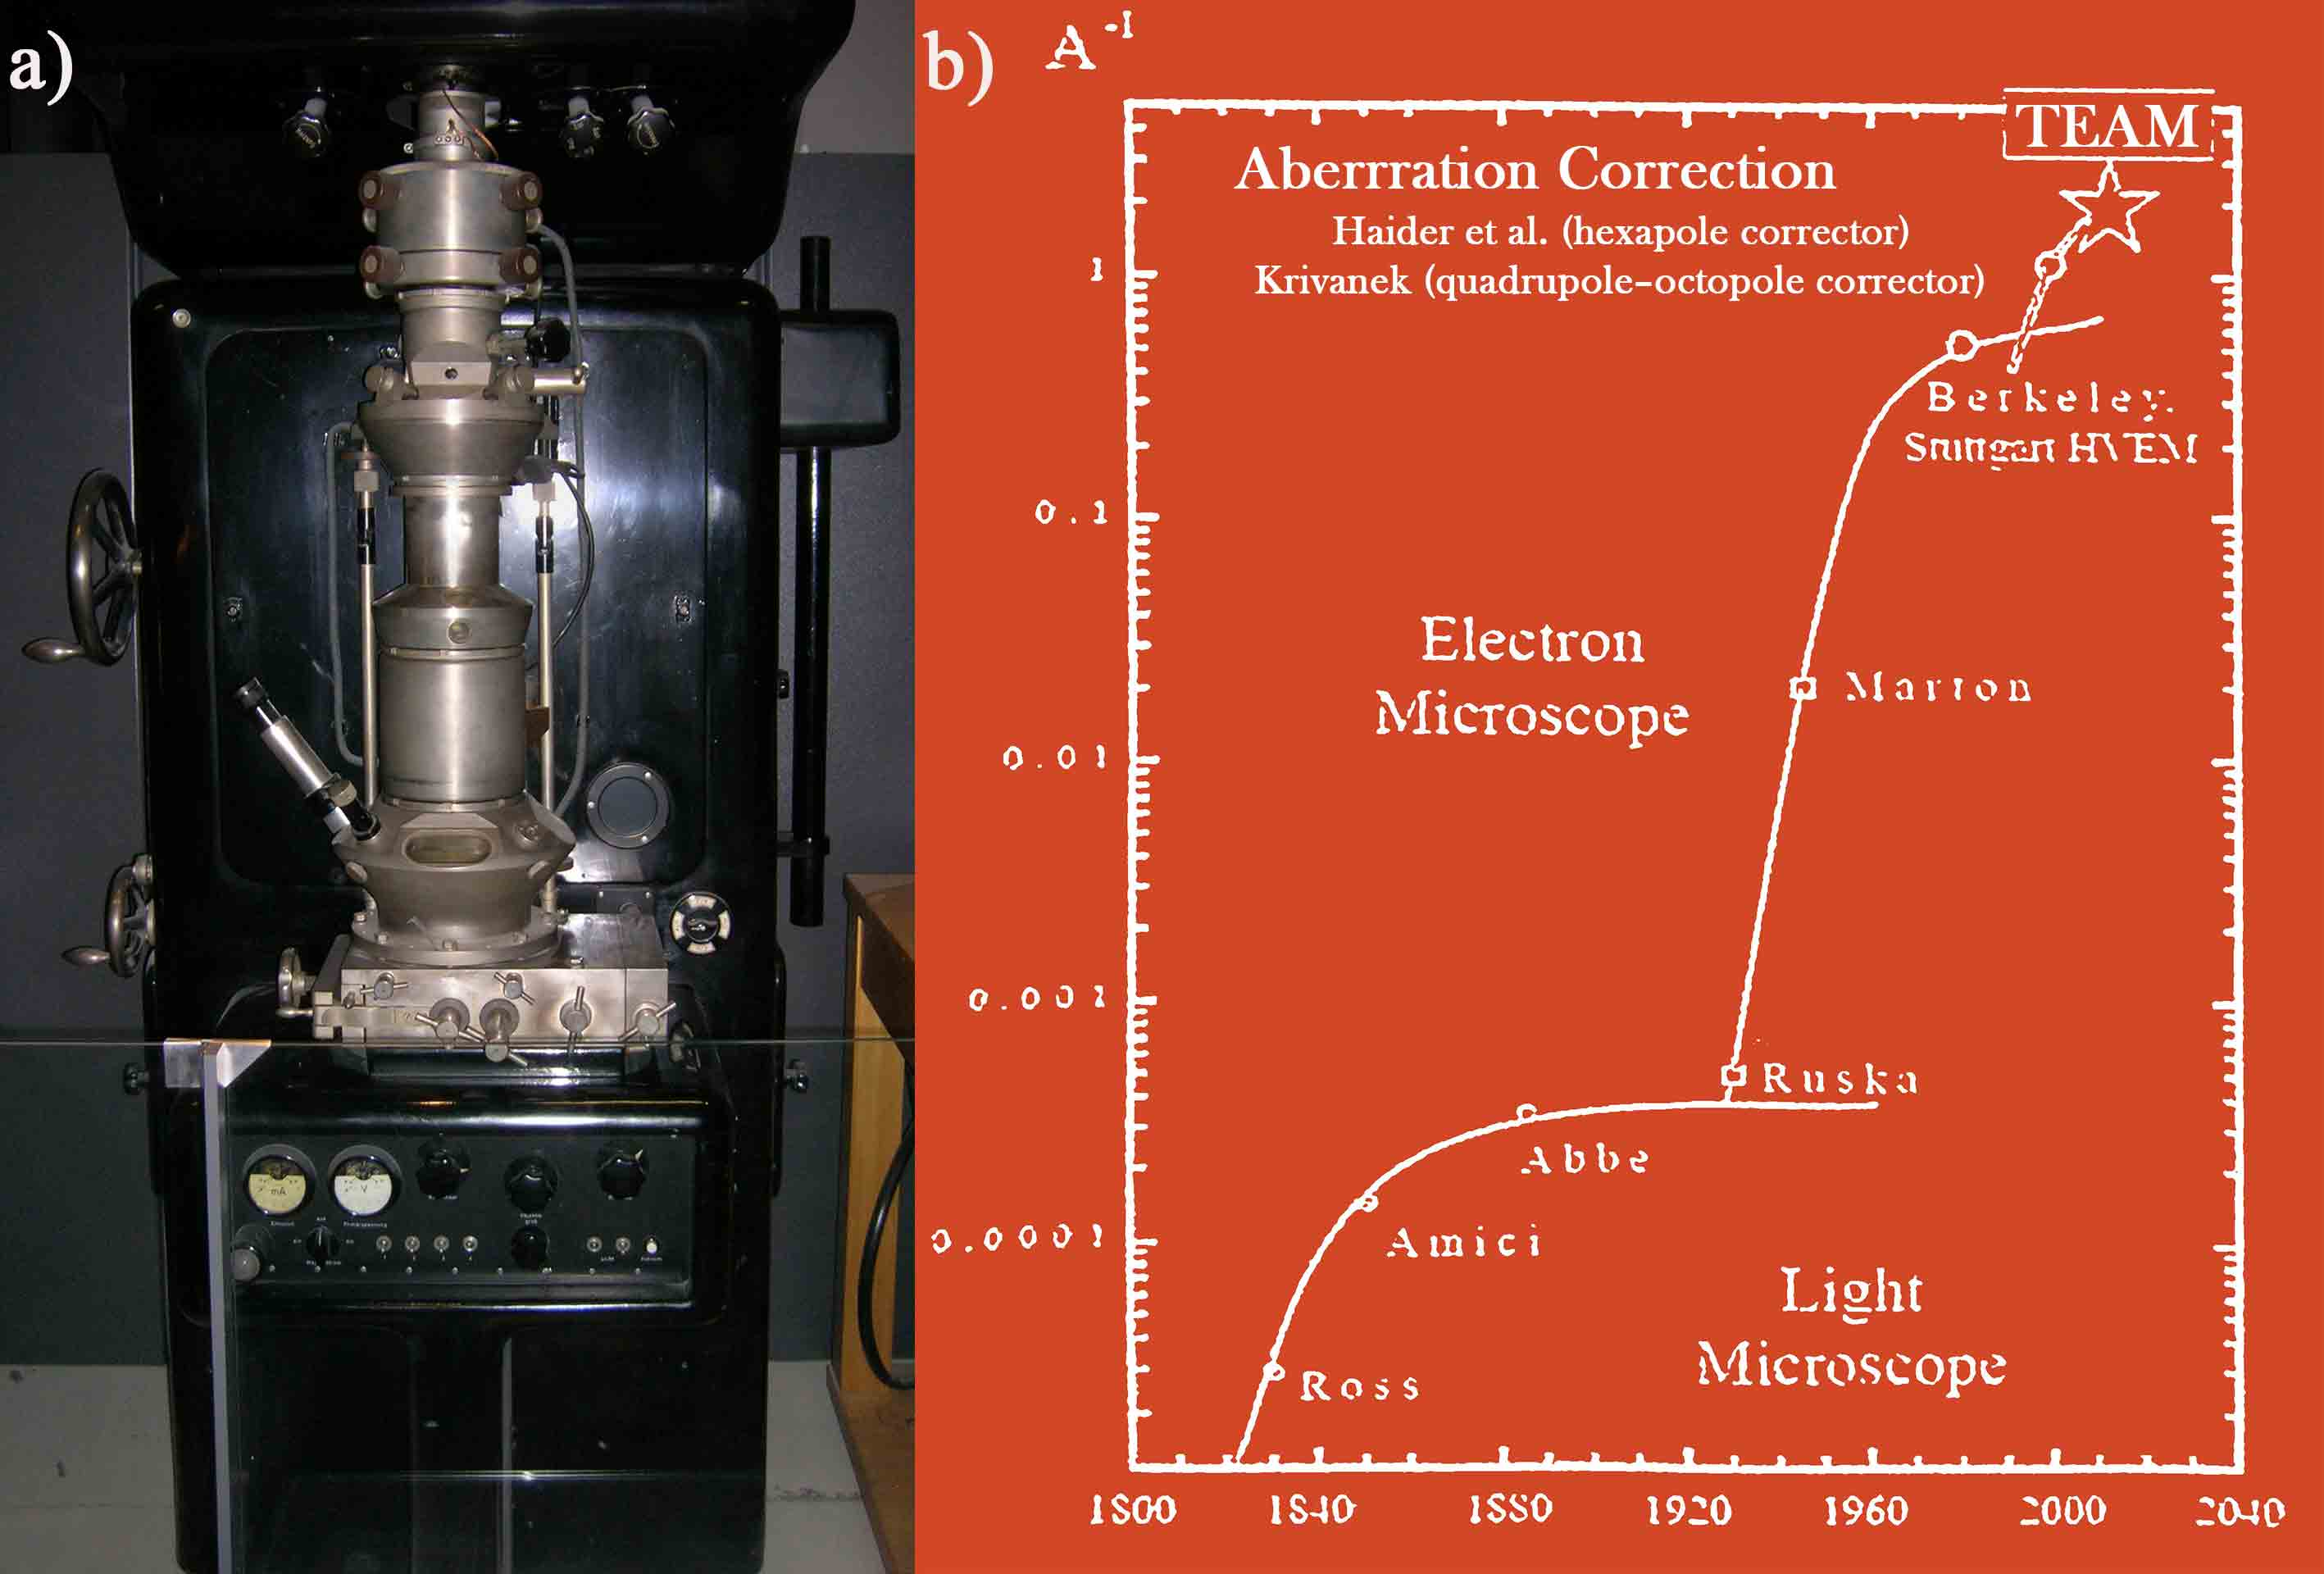
\includegraphics[width=0.8\textwidth]{../1.1/11}
	\caption{世界上第一台电子显微镜与显微镜分辨率发展曲线}\label{fig:11}
	\song\wuhao{a) 世界上第一台电子显微镜;b) 显微镜分辨率发展曲线}
\end{figure}

材料的三维结构对其宏观性能具有很重要的影响。比如铝合金中的析出相的形貌、尺寸以及分布决定其析出强化的效果;纳米颗粒的形貌和尺寸会影响其催化性能、分布状况等。获取材料的三维结构、成分、分布等信息,而不仅仅是二维投影信息,是材料科学研究中一个极其重要的问题。TEM在材料科学领域的应用已经相当广泛,其各种二维原子成像手段更是具有不可替代的作用。TEM在获取材料三维信息方面也具有很多的应用,其手段也是多种多样。三维电子断层扫描[3-7](three-dimensional electron tomography,3DET)技术是应用最广泛的三维重构技术,其基本理论与医学电子计算机断层扫描(computed tomography,CT)的理论相同,通过收集物体多个方向的投影来恢复出物体内部的三维信息。扫描透射电子显微镜(scanning transmission electron microscopy,STEM)以及高角环形暗场(high angle annular dark field,HAADF)成像模式的发明,普及了3DET技术的应用[8-11],并使其能够达到原子分辨率。STEM分辨率的不断提升,还催生了光学层析[10, 12-17]三维重构的运用。但是,这两种三维重构的方法,依然面对着种种问题限制着它们的应用,比如缺失锥[18-25]、辐照损伤[26]、样品漂移[27-30]等等。
% !Mode:: "TeX:UTF-8"
\let\origdoublepage\cleardoublepage
\newcommand{\clearemptydoublepage}{
	\clearpage
	{\pagestyle{empty}\origdoublepage}
}
\clearemptydoublepage
\chapter{一种基于神经网络的 3DET 方法}
\section{引言}
3DET 是 TEM 中常用的重构材料三维结构的技术,它被广泛地应用在催化材料~\cite{Weyland2002}、合金~\cite{Yang2014,Malladi2014,YuXW2020}、生物材料~\cite{Dahlberg2020}等领域。它的常用重构算法有 WBP、ART、SIRT、SART 等。在具有充分的样品投影数据时,这些算法都能精确地重构样品的三维结构与形貌。但是,在 TEM 中,极靴的存在限制了样品杆的可倾转范围,并且样品在倾转至高角度时,它的有效厚度过大导致无法正常成像。这两个原因导致了在 TEM 中无法完整地获得样品从 0° 倾转到 180° 的投影,从而使 3DET 的重构结果中出现缺失锥假象~\cite{Paavolainen2014,Gontard2015}。缺失锥假象不仅会降低重构的分辨率,还会在对样品的形状和尺寸的定量分析中引入误差。

抑制缺失锥假象的方法有很多,最简单和直观的是使用特定的滤波器对重构的结果进行滤波操作~\cite{Kovacik2014}。但是生成这种滤波器需要调节一系列参数,而且它仅能抑制某一种假象,无法全面地抑制缺失锥效应。也有人尝试根据 sinogram 固有的形状直接反推出缺失的投影信息,比如信号外推法~\cite{Yau1996}和轨迹追踪算法~\cite{Kupsch2015}。但是这些方法不完全遵从 3DET 的重构原理,它们会在重构结果种引入额外的假象。更有效的方法是在 3DET 的迭代算法中引入一些先验知识。比如 DART 就是一种行之有效的算法,它在纳米材料的 3DET 重构中有许多应用成果~\cite{Batenburg2009,Bals2007,Biermans2010,Bals2009,Zurner2009,Zhuge2017}。这种方法假设样品的成分是分段连续且有限的,据此,DART 在每次迭代中将重构结果的灰度值离散化。但是有很多情况是不符合这种“离散”假设的,所以 DART 的应用受到很大程度的限制。全变分最小化(total variance minimization,TVM)是一种正则化方法,它利用第 1.3.5 条中介绍的 TV 正则化项~\cite{Persson2001,Rudin1996,Goris1996,Jiang2018}约束重构的结果,具有平滑重构结果和抑制缺失锥假象的作用。TVM 在迭代过程中降低重构结果的“总梯度”,它的使用前提是样品内部的成分连续分布。TVM 常常使重构的结果呈现补丁状,所以会丢失一些样品的细节。

深度学习技术可以通过神经网络引入大量的先验知识来抑制缺失锥假象~\cite{Ding2019,Pelt2013,Bladt2015,YangF2020}。一个训练好的神经网络模型可以快速进行 3DET 重构,并且在有些应用案例中,它可以仅通过 10 张投影图像进行重构~\cite{Bladt2015}。但是,深度学习技术高度依赖于训练集的数据数量和质量,训练成本很高,而且一个训练好的模型只能适用于某一个具体的应用场景。其实,神经网络还有另一种应用于图像重建的方式,它并不使用深度学习技术,而是通过神经网络直接求解线性方程组。早在 90 年代,就有学者研究这种 ART 形式的神经网络图像重建方法~\cite{Srinivasan1993,Ma2000,Deming1998,Cichocki1995,Wang2006,Teranishi2016},但是这些研究集中在 CT 领域,在 3DET 领域中这种方法还鲜为人知。在这些早期的研究中,有些方法同样要结合一定的先验知识或正则化方法~\cite{Deming1998,Cichocki1995,Wang2006,Teranishi2016},但是也有一些方法不使用先验知识也能够获得不错的重构结果~\cite{Srinivasan1993,Ma2000}。目前为止,对这种 ART 形式的神经网络图像重建方法的研究还不彻底,它所具有的潜能还没有被充分挖掘,比如它是否能有效地抑制缺失锥假象还不为人知。

另一方面,在傅里叶空间中,如果缺失的信息占样品总信息的比率较高,那么在实空间中的缺失锥假象就会非常严重。一般情况下,块体材料的 TEM 样品是大纵横比薄片状的,面积很大而厚度很小,并且在倾转投影之前,样品一般垂直于入射电子束放置。这种情况恰恰会造成严重的缺失锥假象,具体原因将在第 2.2 节中详述。这种严重的缺失锥假象,在有些重构的场景中会被忽略,原因是在某些 3DET 的应用中,比如重构铝合金内部的析出相时,内部颗粒的强度往往比基体的强度强很多,所以由基体产生的缺失锥假象容易在数据分析时被忽略或者在重构过程中衰退。但是,在更多的情况下,这种假象是不可忽略的,而且它将对重构的结果产生非常严重的影响。

本章提出了一种基于反传播神经网络的 ART 形式的 3DET 重构(neural network ART,NNART)算法,该算法可以在没有任何先验知识的情况下大幅度地抑制缺失锥假象。第 2.2 节将通过模拟,详细讨论 TEM 中常发生的严重的缺失锥假象。第 2.3 节将详细介绍 NNART 算法和分析 NNART 的重构过程,并且通过模拟和与 TVM 对比,证明它对缺失锥假象的显著的抑制作用。第 2.4 节使用 NNART 重构了盘片状的 SiC 的 TEM 样品,NNART 抑制了严重的缺失锥假象,并正确地重构出了样品中的游离石墨相和 SiC 基体的形貌。第 2.4 节详细讨论了 NNART 与正则化方法之间的关系。

\section{TEM 中严重的缺失锥假象}

缺失锥假象的严重程度与样品的形状、倾转时的几何位置密切相关。在一般的 3DET 实验中,TEM 样品是箔状的,它沿着缺失锥方向的等效厚度很小,而垂直于缺失锥方向的面积却非常大,这种情况将导致非常严重的缺失锥假象。为了更清楚地说明此问题,图 2.1 通过模拟对比了普通情况和 TEM 样品造成的缺失锥假象。图 2.1a 和 b 分别是两个模拟样品,模型 1 和模型 2。模型 1 代表一个立方体纳米颗粒的某一截面,模型 2 代表了一个纵横比为 5 的 TEM 箔状样品的横截面。在这些样品的内部,一些强度较弱的长方形内嵌其中,这增加了样品的复杂程度,同时提高了重构的难度。在 TEM 中,电子束的入射方向一般默认标记为 $z$ 方向,倾转轴沿着 $y$ 方向并且总是图像的中垂线。模型 2 所示的箔状样品在倾转之前一般是横躺着放置在 TEM 中,此时样品沿着 $z$ 方向的有效厚度是最小的。之后,两个模型围绕倾转轴,在倾转角为 -70° 到 +70°,倾转间隔为 1° 的倾转模式下进行倾转投影。最后,使用 SIRT 算法重构这两套倾转系列像,迭代次数是 100 次,重构结果如图 2.1b 和 e 所示。图 2.1c' 和 f' 是图 2.1b 和 e 的傅里叶变换(只展示了中心下半部分),直观地展示了缺失锥。图 2.1b 中清楚地标注了三种缺失锥假象:白色箭头标注的射线假象,红色箭头标注的伸长假象和黑色箭头标注的暗影假象。在图 2.1e 中,TEM 箔状样品中的伸长假象对重构结果是具有破坏性的,它使得整个样品的基体的形状无法辨认。在傅里叶空间中分析该现象,可以更直观地理解其产生的原因。图 2.1c 和 f 展示了模型 1 和模型 2 的傅里叶变换(只展示了中心上半部分),两个模型在傅里叶空间中的信息的强度分布是存在明显的差异的。模型 2 的缺失锥区域内的信息强度占总信息强度的比率高达 76.3\%,而模型 1 的缺失锥区域内的信息占比仅有 29.7\%。所以,在相同的缺失锥条件下,模型 2 损失的信息更多,所以其实空间中的缺失锥假象更加严重。

\begin{figure}[htbp]
	\vspace{\baselineskip}
	\centering
	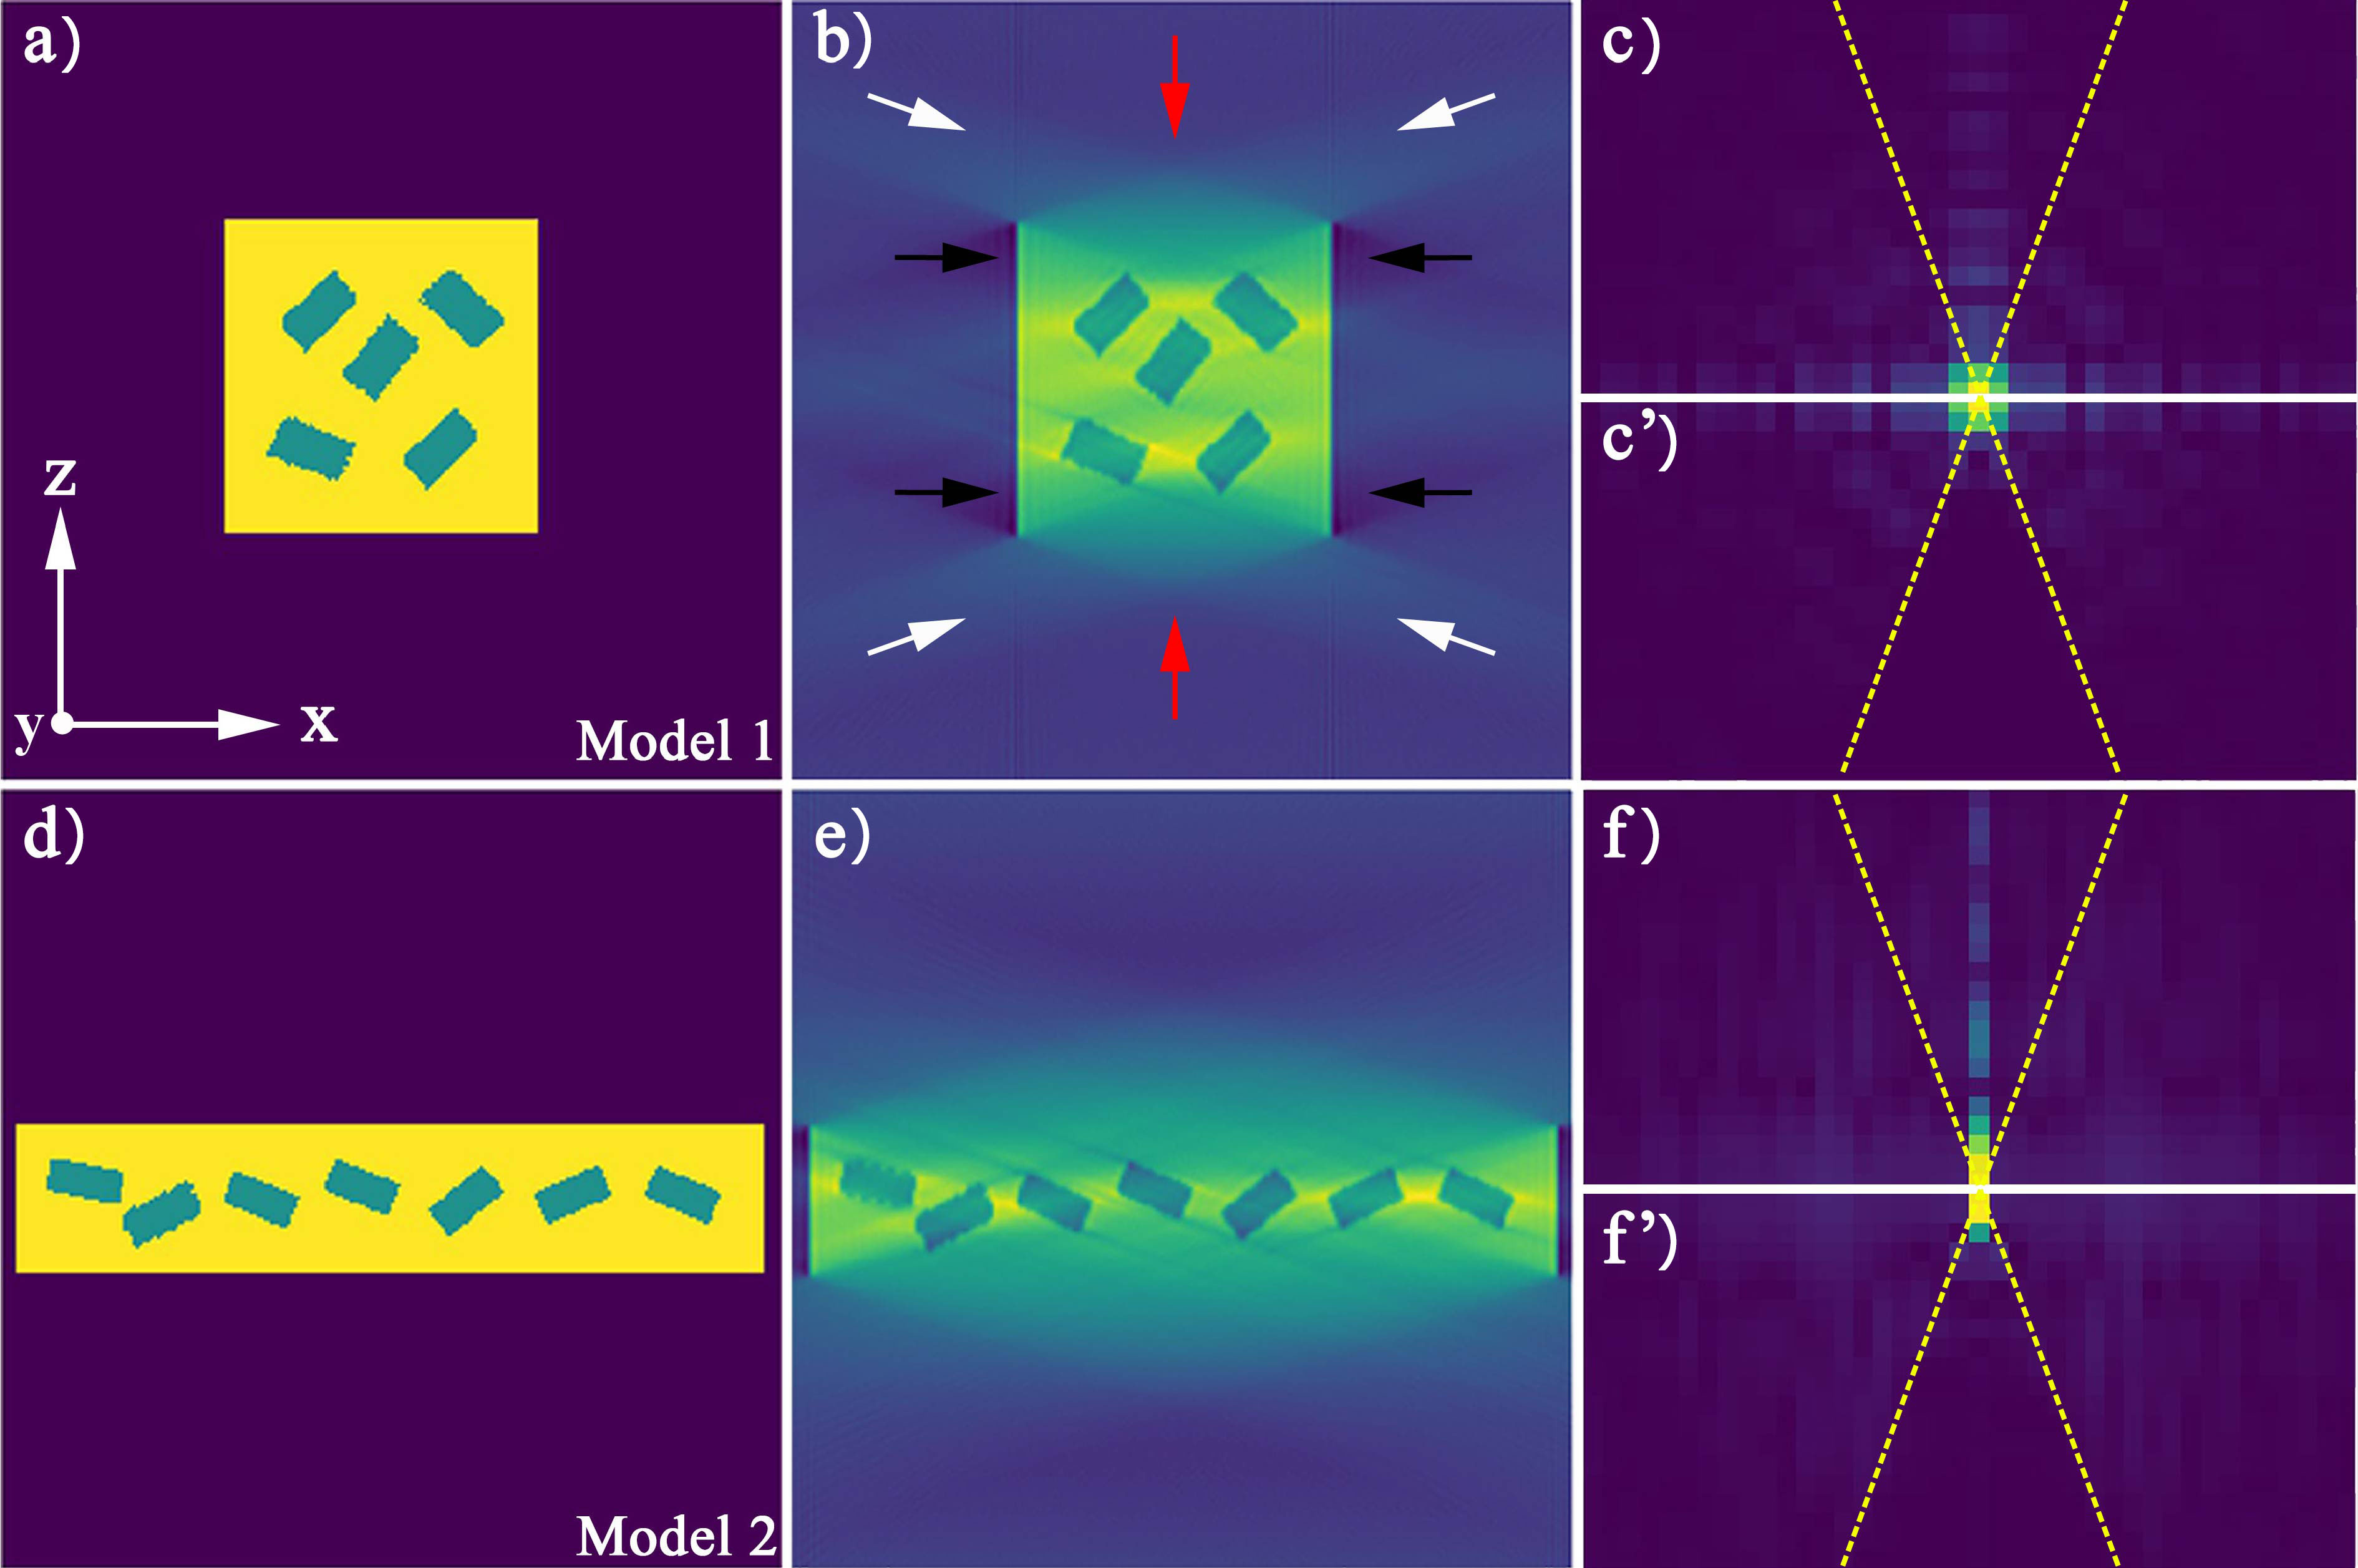
\includegraphics[width=0.9\textwidth]{../3.1/31}
	\caption{TEM 中严重的缺失锥假象图解}\label{fig:31}
	\song\tuzhu{a,d) 模型 1 和模型 2;b,e) 模型 1 和模型 2 的 sinograms 经 SIRT 重构的结果,迭代次数是 100 次,倾转角范围是 -70° 到 +70°,倾转间隔为 1°;c,f) 图 a 和 b 的傅里叶变换(仅显示中心上半部分);c',f') 图 b 和 e 的傅里叶变换(仅显示中心下半部分)}
\end{figure}

\section{NNART 算法和算法测试}
\subsection{算法介绍}

本章提出的 NNART 算法基于广泛使用的反传播神经网络模型~\cite{Rumelhart1986}求解线性方程组:$\boldsymbol{A}\boldsymbol{x}=\boldsymbol{b}$(详情见公式 1.43)。一般,ART 算法的重构过程是使用误差矫正,在迭代过程中使初始值(零或者猜测值)慢慢逼近线性方程组的解。在此基础上,NNART 借助神经网络来完成误差矫正过程,图 2.2a 是 NNART 的流程图。重构的每一次迭代分成三个部分:(i)一个五层的前馈神经网络,如图 2.2b 所示,它的输出层 $\boldsymbol{L}^{(4)}$ 是对应于公式(1.43)中 $\boldsymbol{x}$ 的一维的预测结果;(ii)通过坐标变换得到二维的预测结果,并将其投影,获得 sinogram;(iii)计算损失(loss),然后通过自适应梯度下降算法(adaptive  gradient descent,AdaGrad)优化神经网络中的权重和偏置,使下次迭代中的预测结果更接近正确解。在该算法中,实验投影 sinogram 数据,$\boldsymbol{S}^{exp}$,是在重构时唯一需要获知的信息。重构开始时,算法将使用随机变量对神经网络(包括输入层)进行初始化,当迭代达到一定次数 $t_{max}$ 时重构结束(结束时要保证 loss 收敛)。不过,一次重构的结果往往具有非常大的噪音(如图 2.16a 和 g),这是数值算法本身导致的噪音。为了获得平化解,本算法采用了多次重构取平均值的方法来获得最终结果 $\boldsymbol{I}_{avg}$,其中每次重构的初始化变量都取不同的随机数值。在本章第 2.3 和 2.4 节的研究中,全都取重构 20 次的平均结果。本算法并没有采用更为常用的正则化方法求平滑解~\cite{Aganj2007,Cichocki1995,Skoglund1996},因为探究发现 NNART 在结合了正则化项后,应用时总是受限,这会在第 2.5 节中说明。

\begin{figure}[htbp]
	\vspace{\baselineskip}
	\centering
	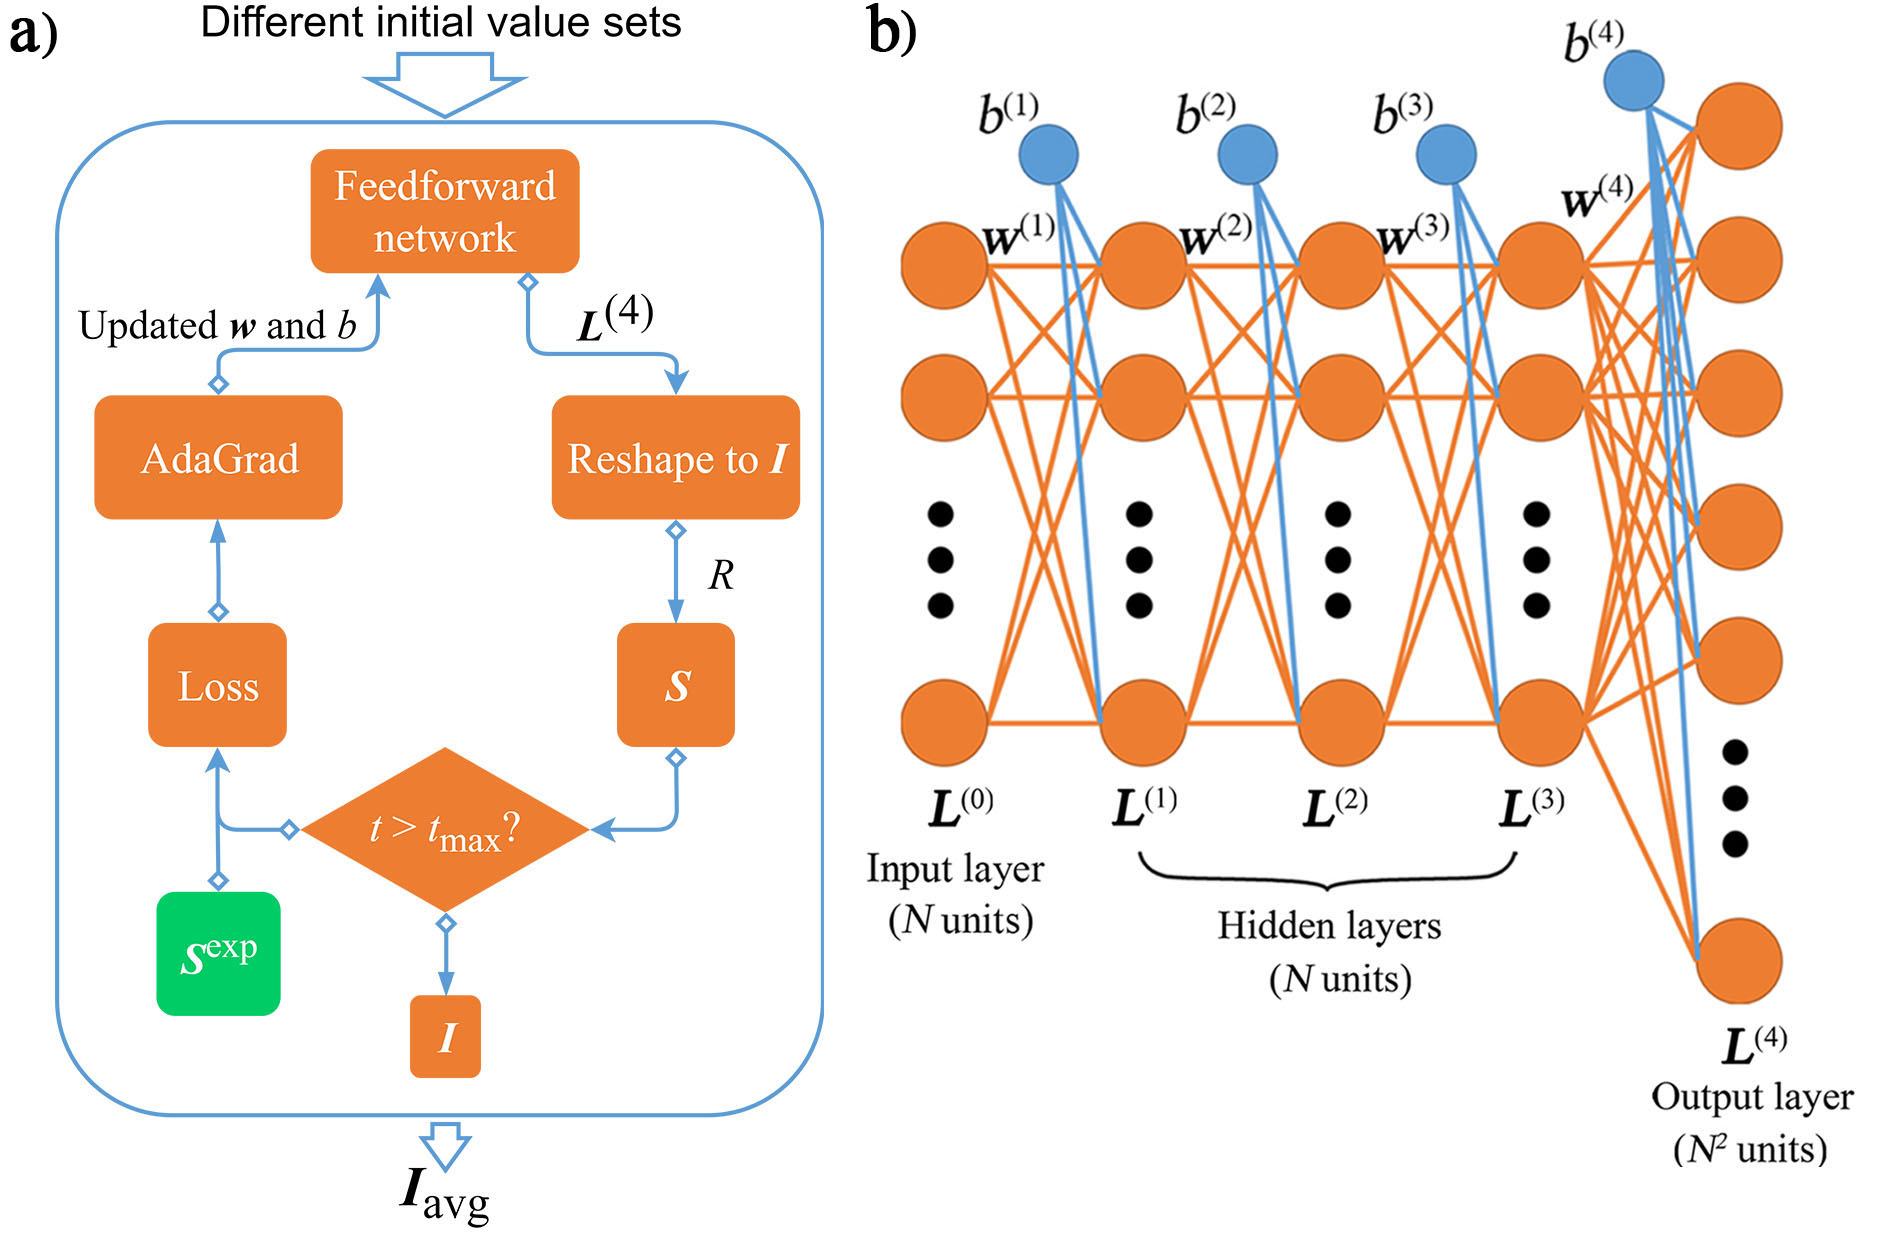
\includegraphics[width=0.9\textwidth]{../3.2/32}
	\caption{NNART 算法示意图}\label{fig:32}
	\song\tuzhu{a) NNART 算法流程图;b) 全连接前馈神经网络的示意图}
\end{figure}

图 2.2b 展示了 NNART 中使用的五层全连接前馈神经网络示意图,它的维度是 $N-N-N-N-N^2$,其中 $N\times N$ 是所需重构的图像的维度。输入层 $\boldsymbol{L}^{(0)}$ 以及所有的权重和偏置将根据截断正态分布的概率进行初始化。相邻两层之间的前向传播公式如下:
\begin{equation}
	\boldsymbol{L}^{(n)}= \sigma \left(\boldsymbol{L}^{(n-1)}\times \boldsymbol{w}^{(n)} + b^{(n)}\right)
\end{equation}
其中 $\boldsymbol{w}^{(n)}$ 和 $b^{(n)}$ 是连接相邻两层的权重和偏置,$\sigma$ 是非线性激活函数,本算法中使用的是 Relu 函数:
\begin{equation}
\sigma(x)= \max(x,0)
\end{equation}
为了实现神经网络的全连接,$\boldsymbol{w}^{(n)}(n = 1, 2, 3)$ 的维度是 $N\times N$ 而 $\boldsymbol{w}^{(4)}$ 的维度是 $N\times N^2$。$b^{(n)} (n = 1\sim 4)$ 是标量变量。

然后,输出层 $\boldsymbol{L}^{(4)}$ 中的元素的坐标会被重新排列得到预测的重构结果 $\boldsymbol{I}$:
\begin{equation}
	\boldsymbol{I}_{[k/N],mod(k,N)}=\boldsymbol{L}^{(4)}_k,k\in Z,0\le k<N^2
\end{equation}
接着,图像 $\boldsymbol{I}$ 通过拉登变换($\mathcal{R}$)进行投影得到 sinogram, $\boldsymbol{S}$:
\begin{equation}
 \boldsymbol{S}=\mathcal{R}(\boldsymbol{I})
\end{equation}
损失函数定义为实验投影 $\boldsymbol{S}^{exp}$ 与预测投影 $\boldsymbol{S}$ 之间的绝对误差的根号的求和:
\begin{equation}
L=\sum \sqrt{|\boldsymbol{S} - \boldsymbol{S}^{exp}|}
\end{equation}
最后,根据梯度下降法,沿着使损失 $L$ 变小的梯度更新权重和偏置,使下次迭代中的预测结果更接近正确解,梯度下降法的公式如下:
\begin{equation}
w^{(n)(t+1)}_{i,j}=w^{(n)(t)}_{i,j}-\eta \left.\frac{\partial L}{\partial w^{(n)}_{i,j}}\right|_{w^{(t)}}
\end{equation}
\begin{equation}
b^{(n)(t+1)}=b^{(n)(t)}-\eta \left.\frac{\partial L}{\partial b^{(n)}}\right|_{b^{(t)}}
\end{equation}
其中 $t$ 是迭代次数,$\eta$ 是学习率。在本算法中,使用了自适应梯度下降算法,它在迭代过程中能够自动调整学习率。

本章中 NNART 的实现使用了自研的 Python 代码,其中神经网络的运算通过 Tensorflow~\cite{Abadi2016} 模块实现。

\subsection{重构过程}
本条以模型 1 为例,详细描述 NNART 的重构过程,促进对其重构原理的理解。原始模型如图 2.1a 所示,像素大小是 $256\times 256$,然后模型在 -70° 至 +70° 的倾转角,倾转间隔为 1° 的条件下被投影。随后,投影数据使用 NNART 进行重构,重构结果如图 2.3 所示。

图 2.3a 展示了重构过程中 loss 的收敛曲线(纵坐标使用对数标尺)。由于重构开始时的神经网络是随机赋值初始化的,所以预测结果和真实的实验数据之间的偏差非常大,loss 值接近 10$^4$。随后,loss 在若干次迭代内大幅度下降,这意味着该过程中权重和偏置的变化幅度很大。尽管如此,如图 2.3b 所示,此时的预测结果仍然呈现随机噪音。当迭代次数到达 40 次后,loss 下降的速度将减缓。此时的重构结果,正方形样品的大致轮廓开始出现,且相较于图 2.3b 噪音减少了很多,但是样品的内部细节还没有展现出来。图 2.3d 展示了迭代次数到达 400 次时的重构结果。在这个阶段,重构结果和模型 1(图2.1a)接近了很多,但是此时存在着相当严重的射线和伸长假象,而且重构对象的边界非常模糊。不过,暗影假象已经得到了一定程度的抑制,而且图像的背景非常干净,几乎没有噪音。最后,在迭代次数到达 3000 次时,loss 收敛,重构结束。图 2.3e 展示了最终的重构结果,重构对象的边界和和内部的截面都非常清晰,而且缺失锥假象几乎被去除了。

\begin{figure}[htbp]
	\vspace{\baselineskip}
	\centering
	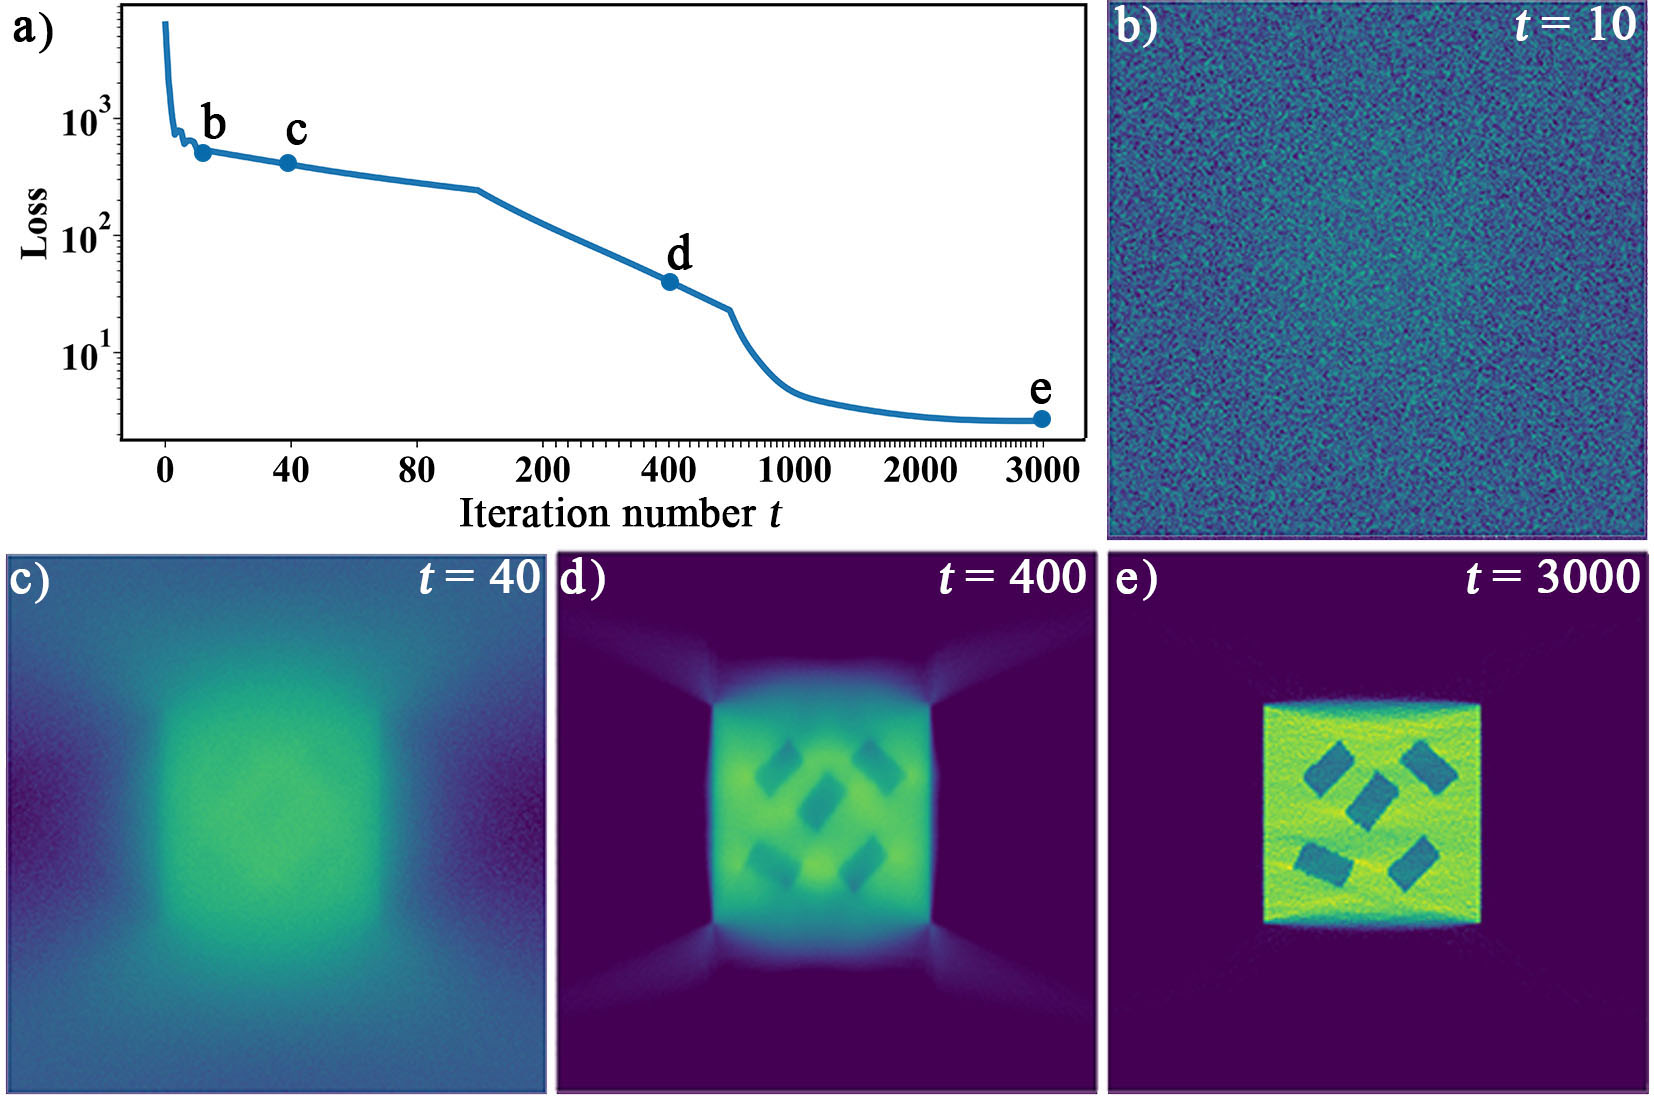
\includegraphics[width=0.9\textwidth]{../3.3/33}
	\caption{NNART 的重构过程}\label{fig:33}
	\song\tuzhu{a) 重构过程中 loss 的收敛曲线,其中纵轴是对数坐标;b-e) 不同迭代次数的重构结果:b) 10,c) 40,d) 400,e) 3000;图 a-e 都是 20 次重构平均的结果}
\end{figure}

图 2.4a-e 对比了模型 1(图2.1a)和图 2.3b-e 中的重构结果的傅里叶变换(仅展示中心右半部分)。显然,随着迭代次数的增加,重构的信息逐渐增多,并且缺失锥中的信息也在一定程度上被重构出来。图 2.4f 定量地对比了图 2.4a-e 沿 $z$ 方向的重构信息的强度。在迭代次数到达 400 时,如图 2.4d 所示,缺失锥以外的区域已经在一定程度上恢复出一些信息,但是沿 $z$ 方向重构的信息仍极为有限的。最终 3000 次迭代恢复出的信息和模型 1 沿 $z$ 方向的信息在低频部分相当接近,并且在高频部分仍具有和模型 1 相同的趋势,这说明重构的信息是正确的。但是,重构的信息沿着 $z$ 方向最终会衰减至无,所以 NNART 无法重构出更高频率的信息,所以在 $z$ 方向上的重构分辨率依然将低于 $x$ 方向的重构分辨率。

总体而言,NNART 在抑制缺失锥假象上的效果是非常显著的,它能够正确地恢复出缺失锥中的信息。这种优异的性能应归功于复杂的神经网络。因为在 NNART 的每一次迭代中,实验数据的信息将通过神经网络的非线性变换,被映射到高维空间中(~$\sim N^3$ 维度的神经网络),然后再经梯度下降算法和前馈传播,对重构结果进行修正。这种先升维再降维的方式,相比于仅在低维空间进行误差修正的 ART 算法,具有更好的求解效果,所以即使没有使用任何先验知识,也能抑制缺失锥假象。

\begin{figure}[htbp]
	\vspace{\baselineskip}
	\centering
	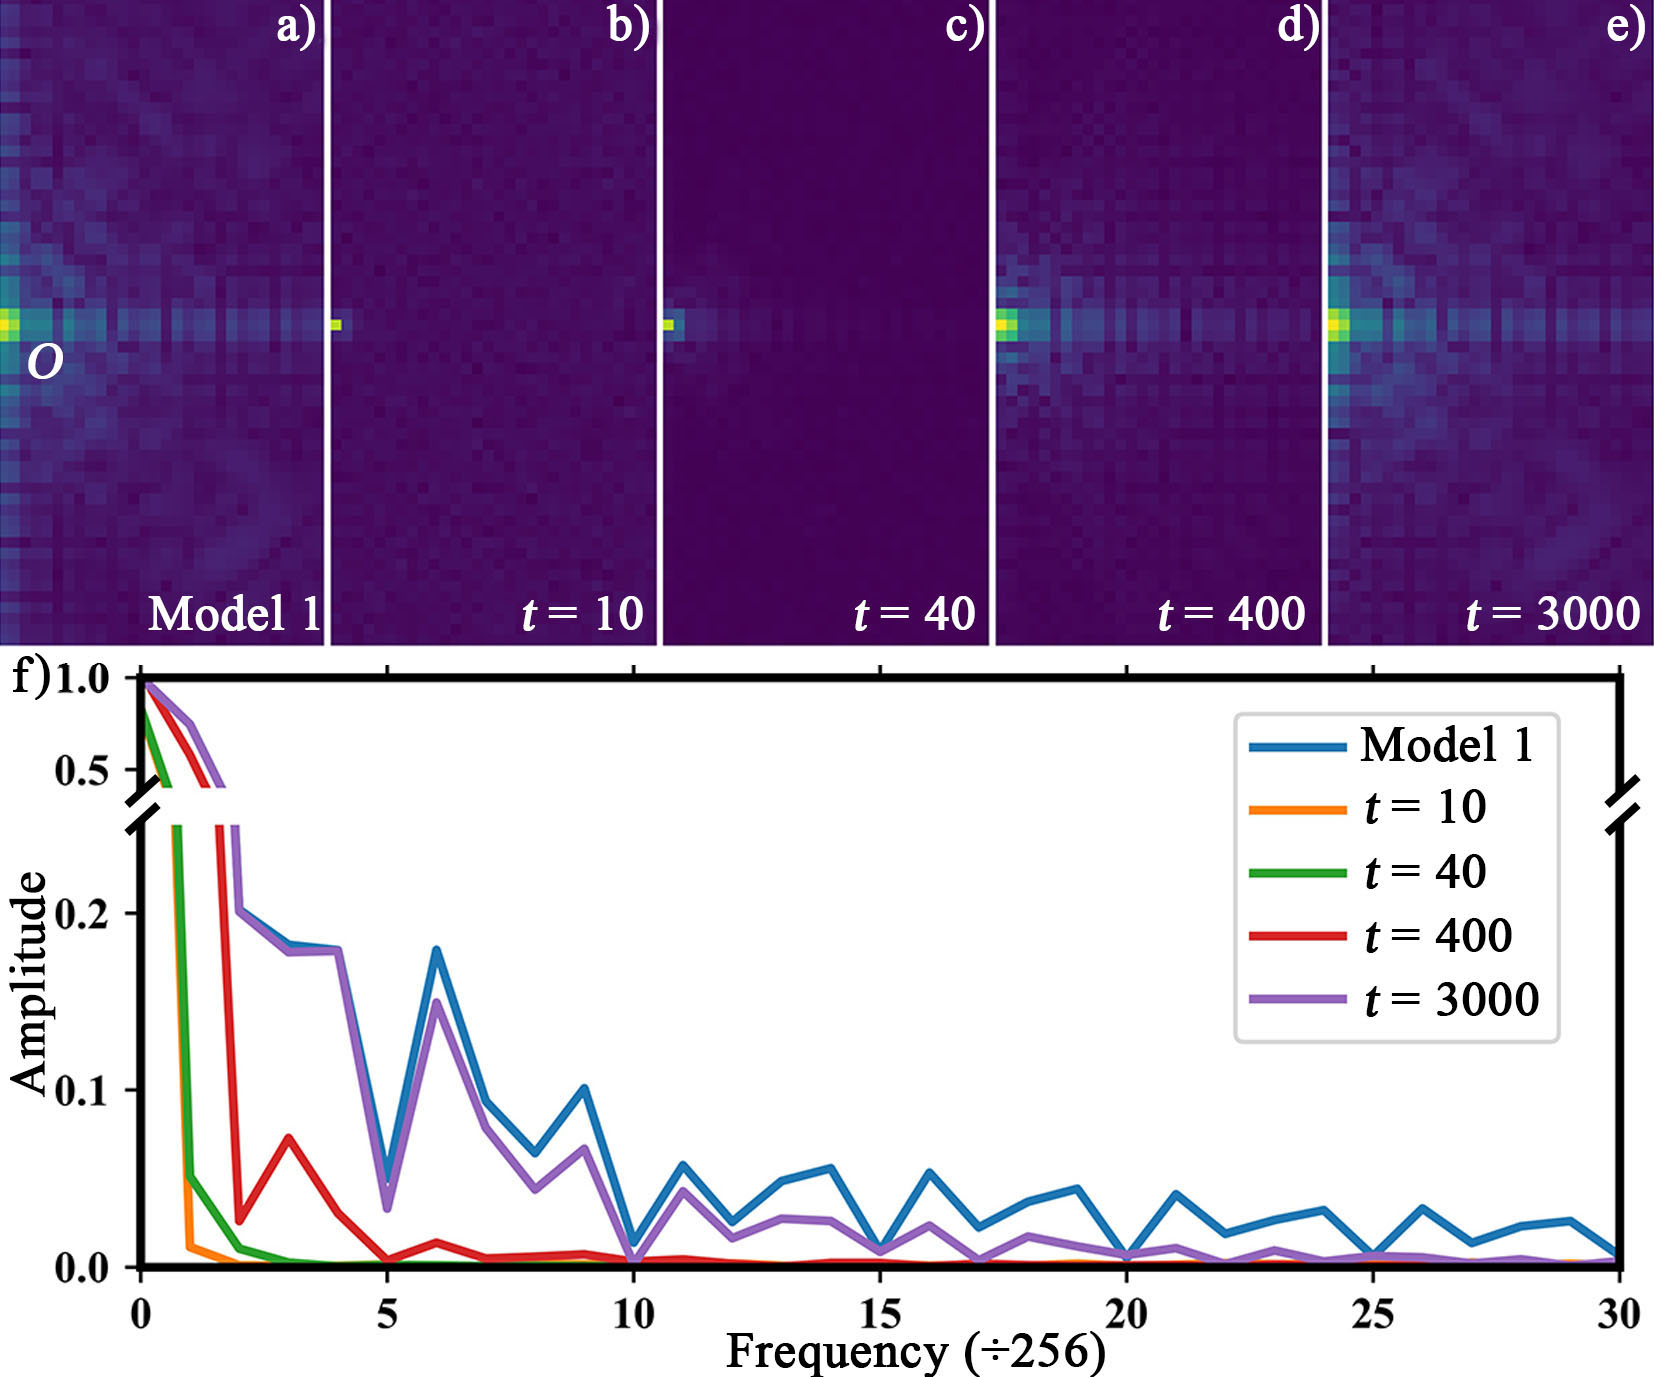
\includegraphics[width=0.9\textwidth]{../3.4/34}
	\caption{不同迭代次数的重构结果的傅里叶变换及分析}\label{fig:34}
	\song\tuzhu{a) 模型 1 的傅里叶变换;b-e) 迭代次数分别维 10,40,400,3000 的重构结果的傅里叶变换;傅里叶变换仅展示了中心右半部分(60  像素 $\times $ 30 像素),且显示于同一灰度衬度下;f) 图 a-e 沿 $z$ 轴的振幅对比曲线}
\end{figure}

\subsection{模拟测试}
图 2.5 展示了不同倾转角范围下,用两种算法重构模型 2 的结果。图 2.5a 和 e 说明了当倾转角范围是 -70° 至 70° 时,NNART 和 TVM 均能有效抑制缺失锥假象。当倾转角范围减小时,图 2.5b-d 和 f-h 中的重构结果中沿 $z$ 方向的伸长假象都会变严重,而且内部的矩形会丢失一些局部细节,不过整个模型都能保持完整。而且,内部的小矩形产生的射线假象变得越来越严重,在 TVM 的重构结果中,这些假象会使结果的补丁状样貌更加明显。相对而言,TVM 抑制伸长假象的效果不及 NNART,而且图 2.5f-h 中在拉伸假象的边界上还存在明显的暗衬度。相反,NNART 的重构结果的总体形状与模型 2 更加接近,而且整体观感比 TVM 的结果更清晰。不过,在 NNART 的重构结果中,当倾转角范围变小后,某些内部小矩形的角上出现了一些小孔,如图 2.5b-d 中白色箭头所标注。这些孔洞的出现,是神经网络的过拟合造成的。当实验数据减少时,过拟合更容易发生,此时神经网络可能会把一些细节当作特征放大。

\begin{figure}[htbp]
	\vspace{\baselineskip}
	\centering
	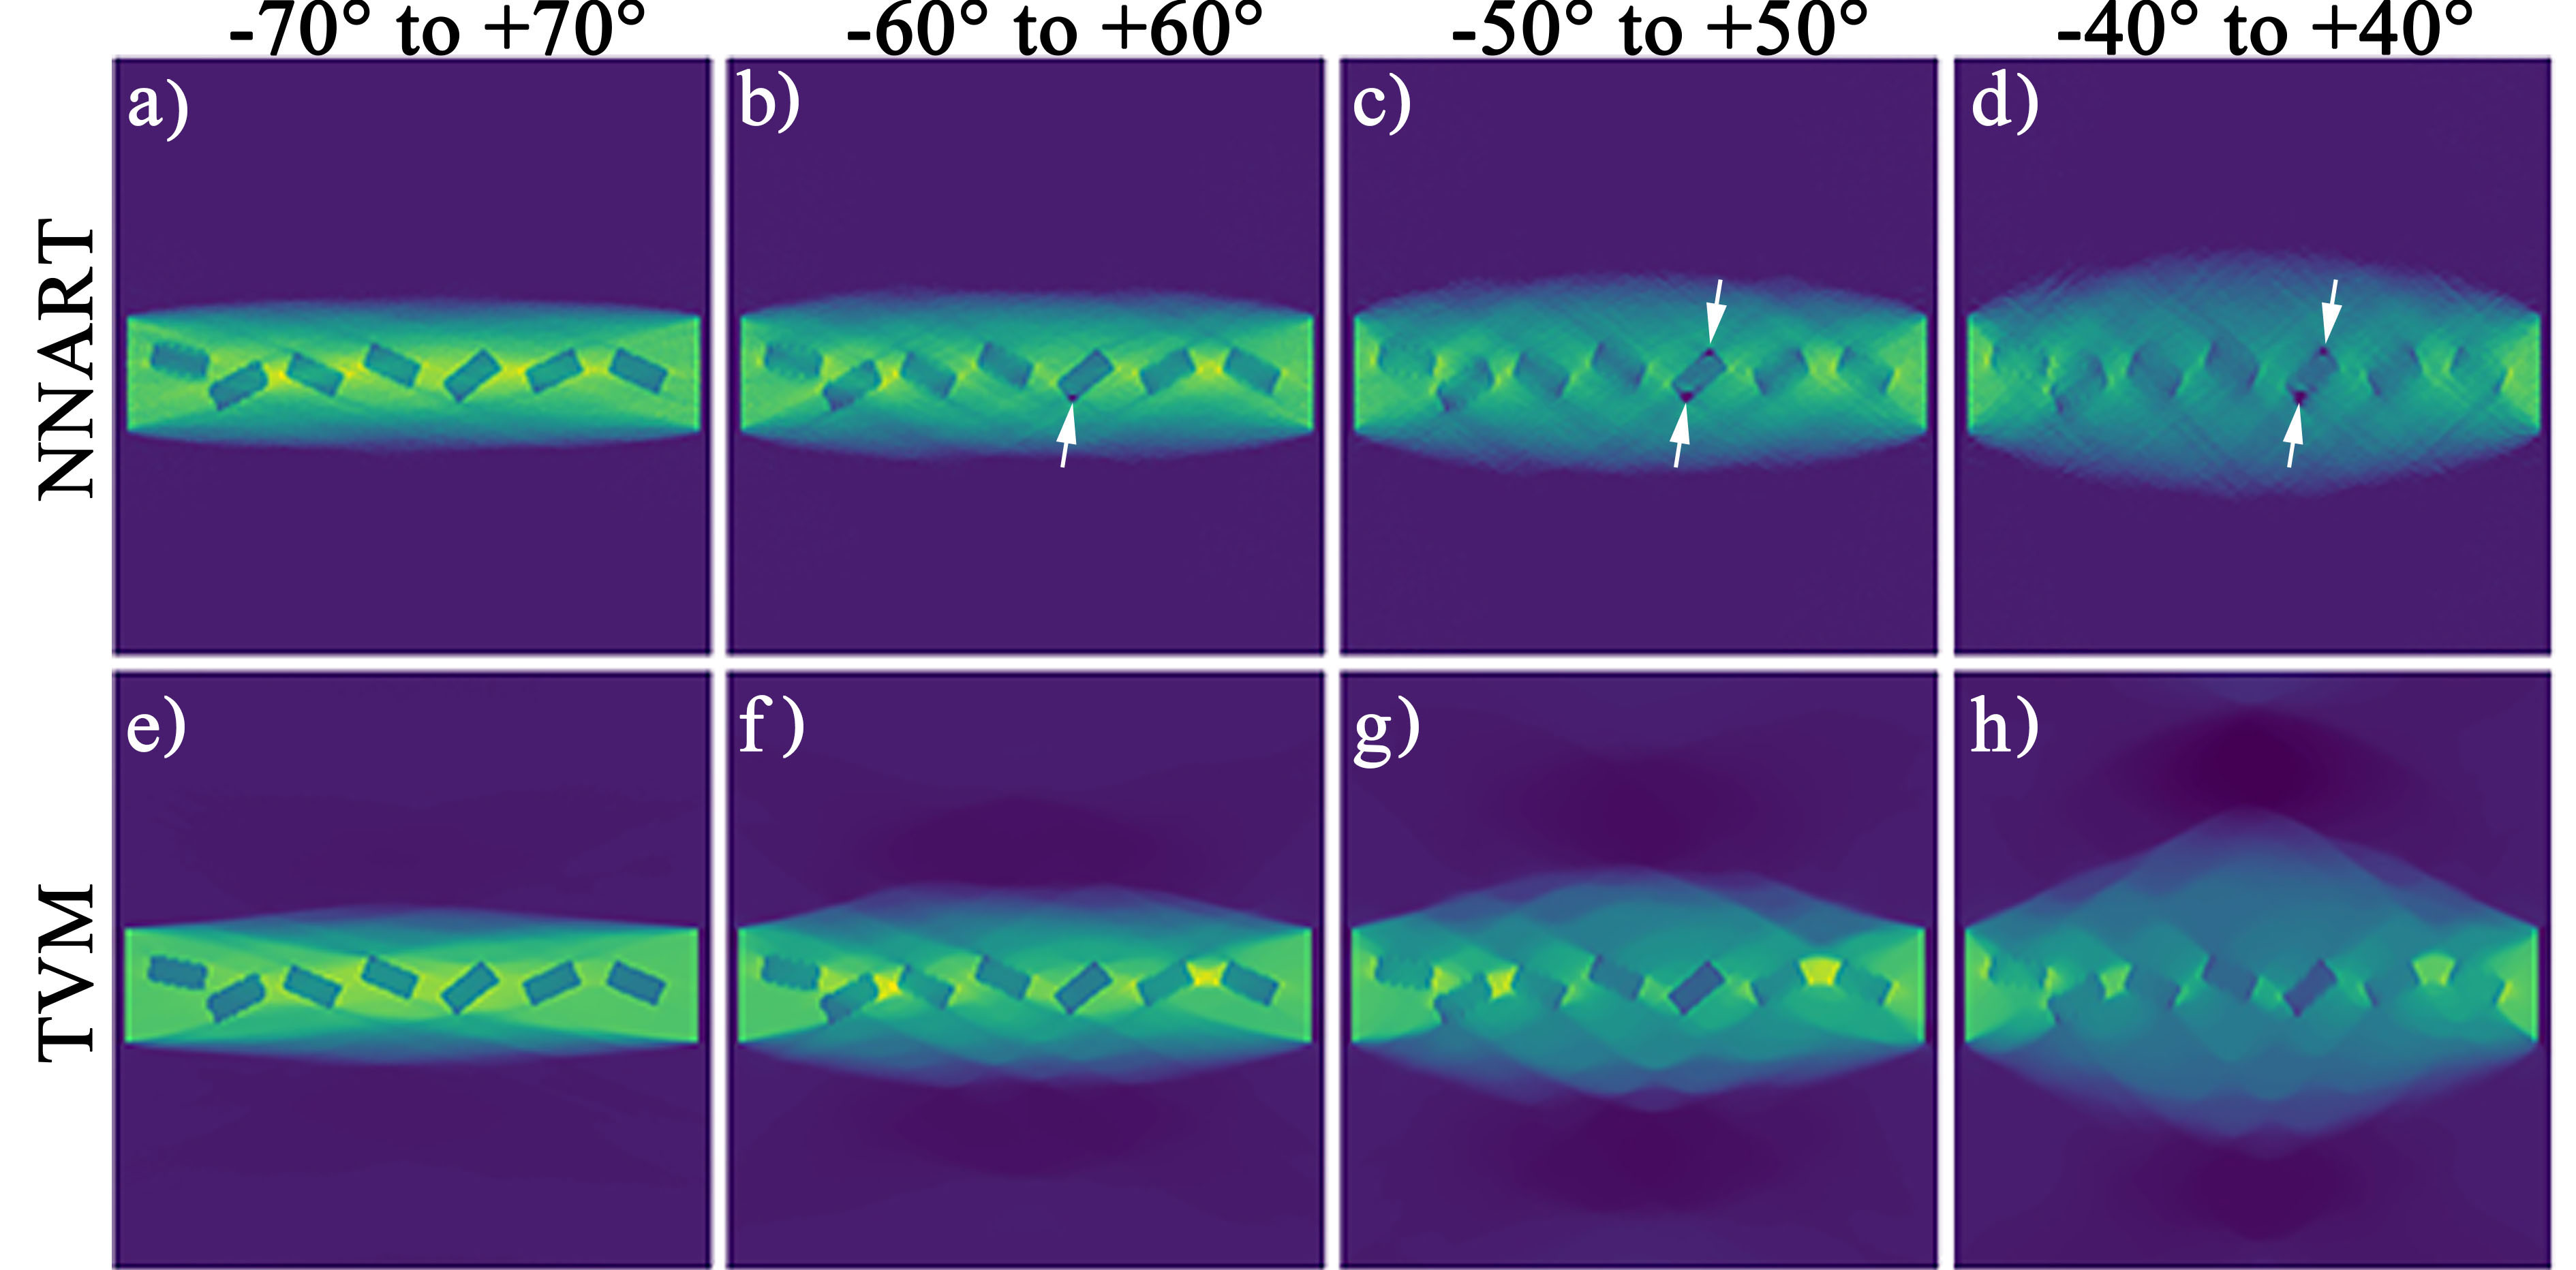
\includegraphics[width=0.9\textwidth]{../3.5/35}
	\caption{不同倾转角范围下 NNART 和 TVM 重构结果对比}\label{fig:35}
	\song\tuzhu{其中倾转角范围分别是:a,e) -70° 至 +70°;b,f) -60° 至 +60°;c,g) -50° 至 +50°;d,h) -40° 至 +40°;倾转间隔均为 1°,NNART 和 TVM 的迭代次数分别是 6000 次和 5000 次,以保证算法收敛;所有图像均显示于同一灰度衬度进行对比}
\end{figure}

噪音是一个无法在实验中避免的降低重构质量的因素。特别地,噪音是否会影响算法对缺失锥假象的抑制,是一个需要在此重点考虑的问题。图 2.6a 和 d 展示了在模型 2 的 sinogram 中加入信噪比(signal noise ratio,SNR)分别为 30 和 20 的泊松噪音后的局部图像。图 2.6b,e,c,f 展示了使用 NNART 和 TVM 重构倾转角范围为 -60° 至 +60° 的带有噪音的 sinogram 的结果。很显然,相比于无噪音时的重构结果(图 2.5b 和 f),不同程度的噪音出现在了相应的重构结果中。不过,对于 NNART 的重构结果而言,图 2.6b 和 e 与图 2.5b 相比,除了噪音没有明显的不同,这意味着噪音并不影响 NNART 对缺失锥假象的抑制作用。反观 TVM 的重构结果,当信噪比是 20 时,整个重构图像中都有严重的噪音,连原有的补丁状特征都消失了,而且块体模型也变得难以辨认。

以上结果证明 NNART 据有非常好的抗噪音能力,其原因可分为两点:首先,
如第 2.2.2 条中所述,复杂的神经网络使得重构更有效。其次,NNART 中使用多次重构平均的方法来求解平滑解,而非使用正则化等方法。使用多次重构平均的方法其实是通过统计的方式来去除数值算法带来的噪音。而因为实验数据是唯一的,所以多次重构平均方法和实验数据中本身存在的噪音是无关的,即实验数据中的噪音不容易影响到重构的过程。反观一些正则化方法无法避免正则化项对实验噪音的作用,所以实验噪音也会相应地影响重构结果。

\begin{figure}[H]
	\vspace{\baselineskip}
	\centering
	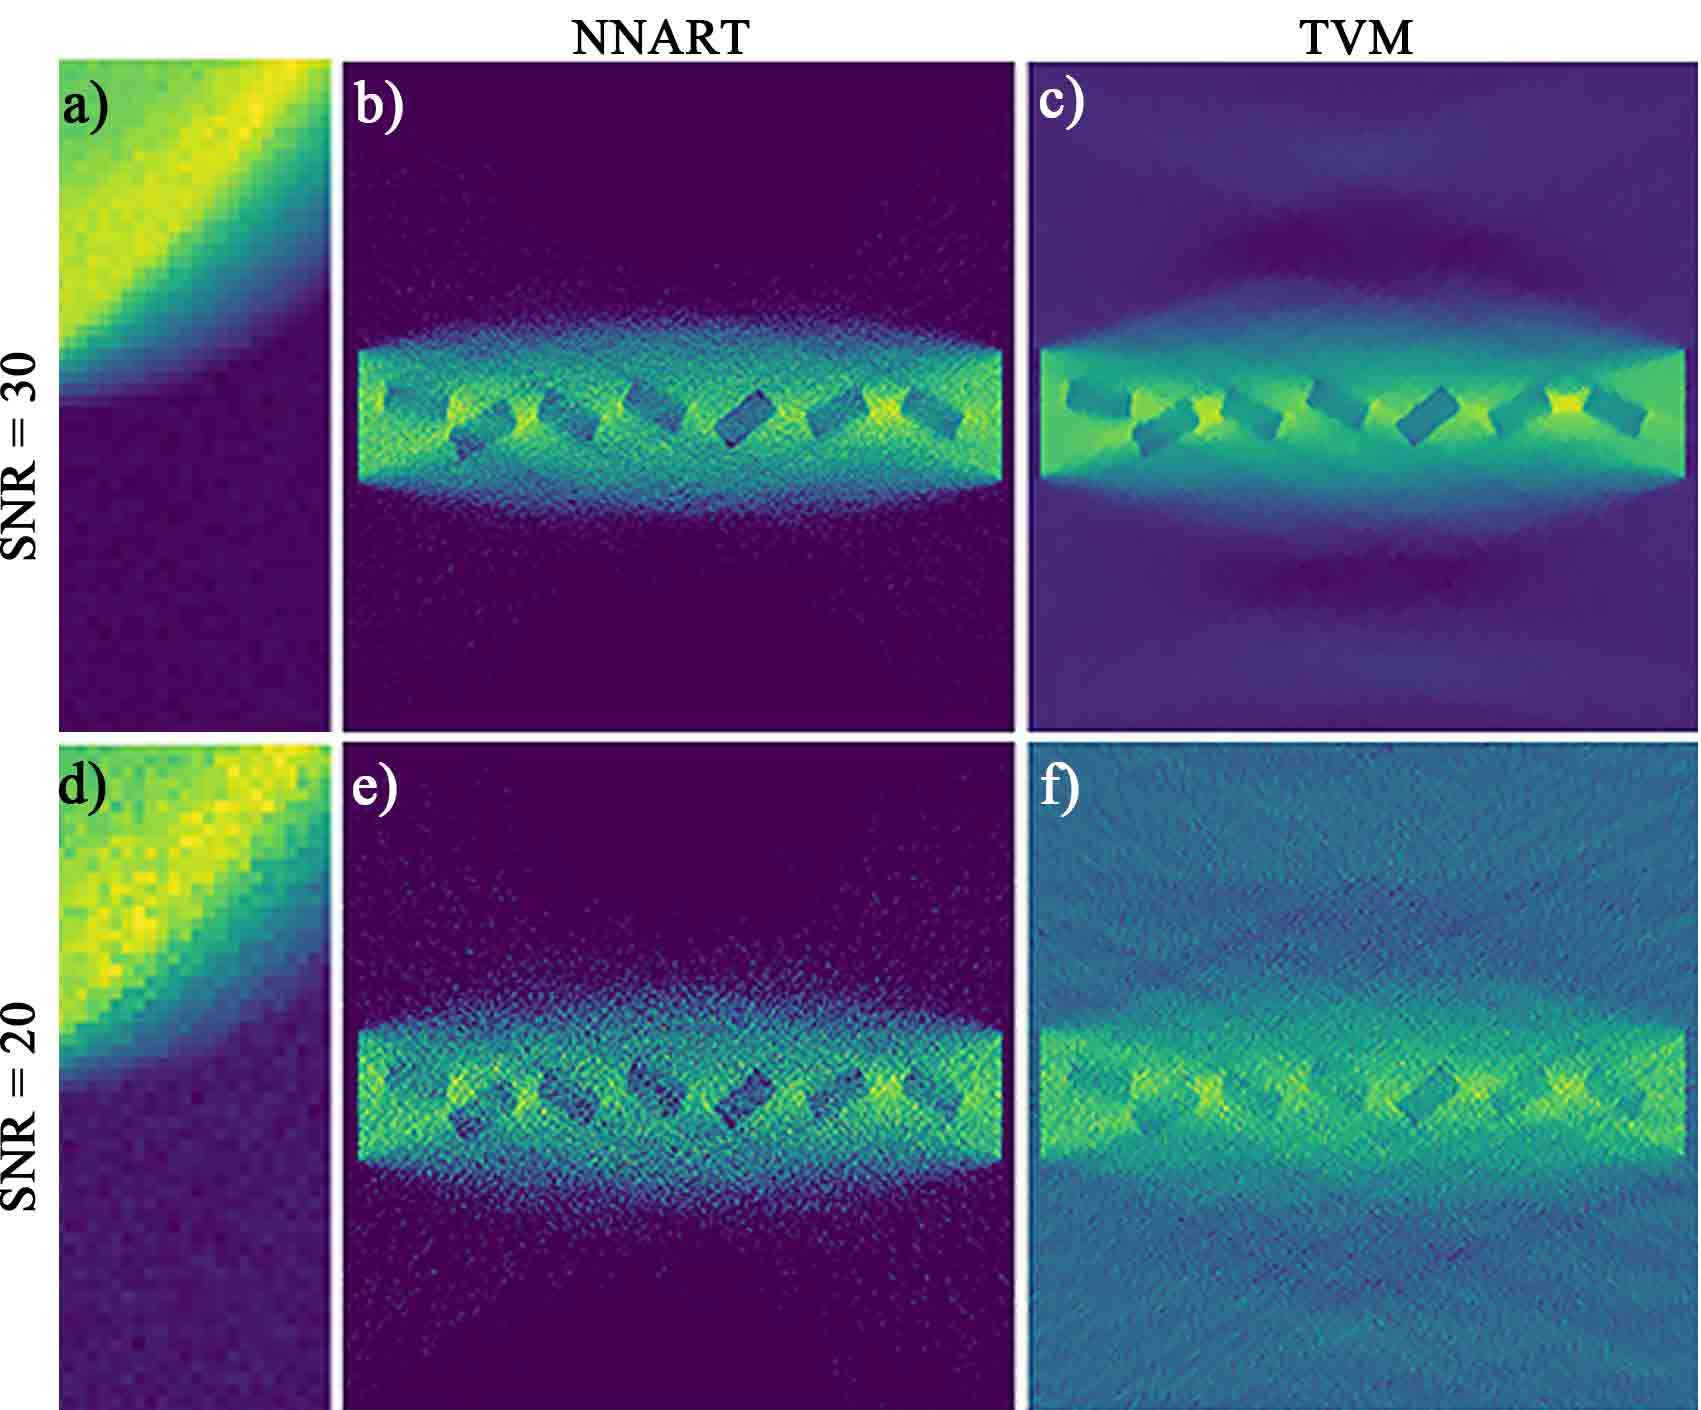
\includegraphics[width=0.9\textwidth]{../3.6/361}
	\caption{噪音对重构的影响}\label{fig:36}
	\song\tuzhu{a,d) 加入信噪比为 30 和 20 的泊松噪音后的 sinogram 的局部示意图;b,c) NNART 和 TVM 重构的加入信噪比为 30 的泊松噪音后的模型 2 的 sinogram 的结果;e,f) NNART 和 TVM 重构的加入信噪比为 20 的泊松噪音后的模型 2 的 sinogram 的结果;sinogram 的倾转角范围是 -60° 至 +60°}
\end{figure}

纳米颗粒是热门的研究对象。当许多纳米颗粒分散在某一区域中时,面对这些颗粒的投影强度的相互影响,NNART 是否还能正常地重构它们,并抑制缺失锥假象,也是一个值得探讨的问题。图 2.7c 是一簇纳米颗粒模型,颗粒形状是纵横比各异的圆角矩形,颗粒在图中呈不同强度,代表它们具有不同的元素成分。图 2.7a 和 b 分别是用 NNART 和 FBP 重构倾转角为 -70° 到 +70° 的 sinogram 的结果。在 FBP 的重构结果中,缺失锥假象非常严重,每个颗粒的两侧都有暗影假象,且射线假象和拉伸假象也很明显。而在图 2.7a 中,缺失锥假象得到了很好的控制,颗粒轮廓分明。对比图 2.7d-f,可知 NNART 重构了大部分缺失锥中原本丢失的信息,且图 2.7d 和 2.7f 非常相似。为了进一步分析恢复的信息的准确性,图 2.7g 和 h 定量对比了图 2.7d 和 f 沿 $z$ 轴和 $x$ 轴的强度。图 2.7h 中两条曲线吻合得很H,H,这是因为沿 $x$ 方向不存在缺失锥, NNART 能够非常准确地重构该方向上的信息。而在图 2.7g 中,沿 $z$ 方向,NNART 重构的信息的强度与原始的强度也基本吻合,仅在频率较高时开始衰减。所以,NNART 能够很好地重构纳米颗粒。


\begin{figure}[H]
	\vspace{\baselineskip}
	\centering
	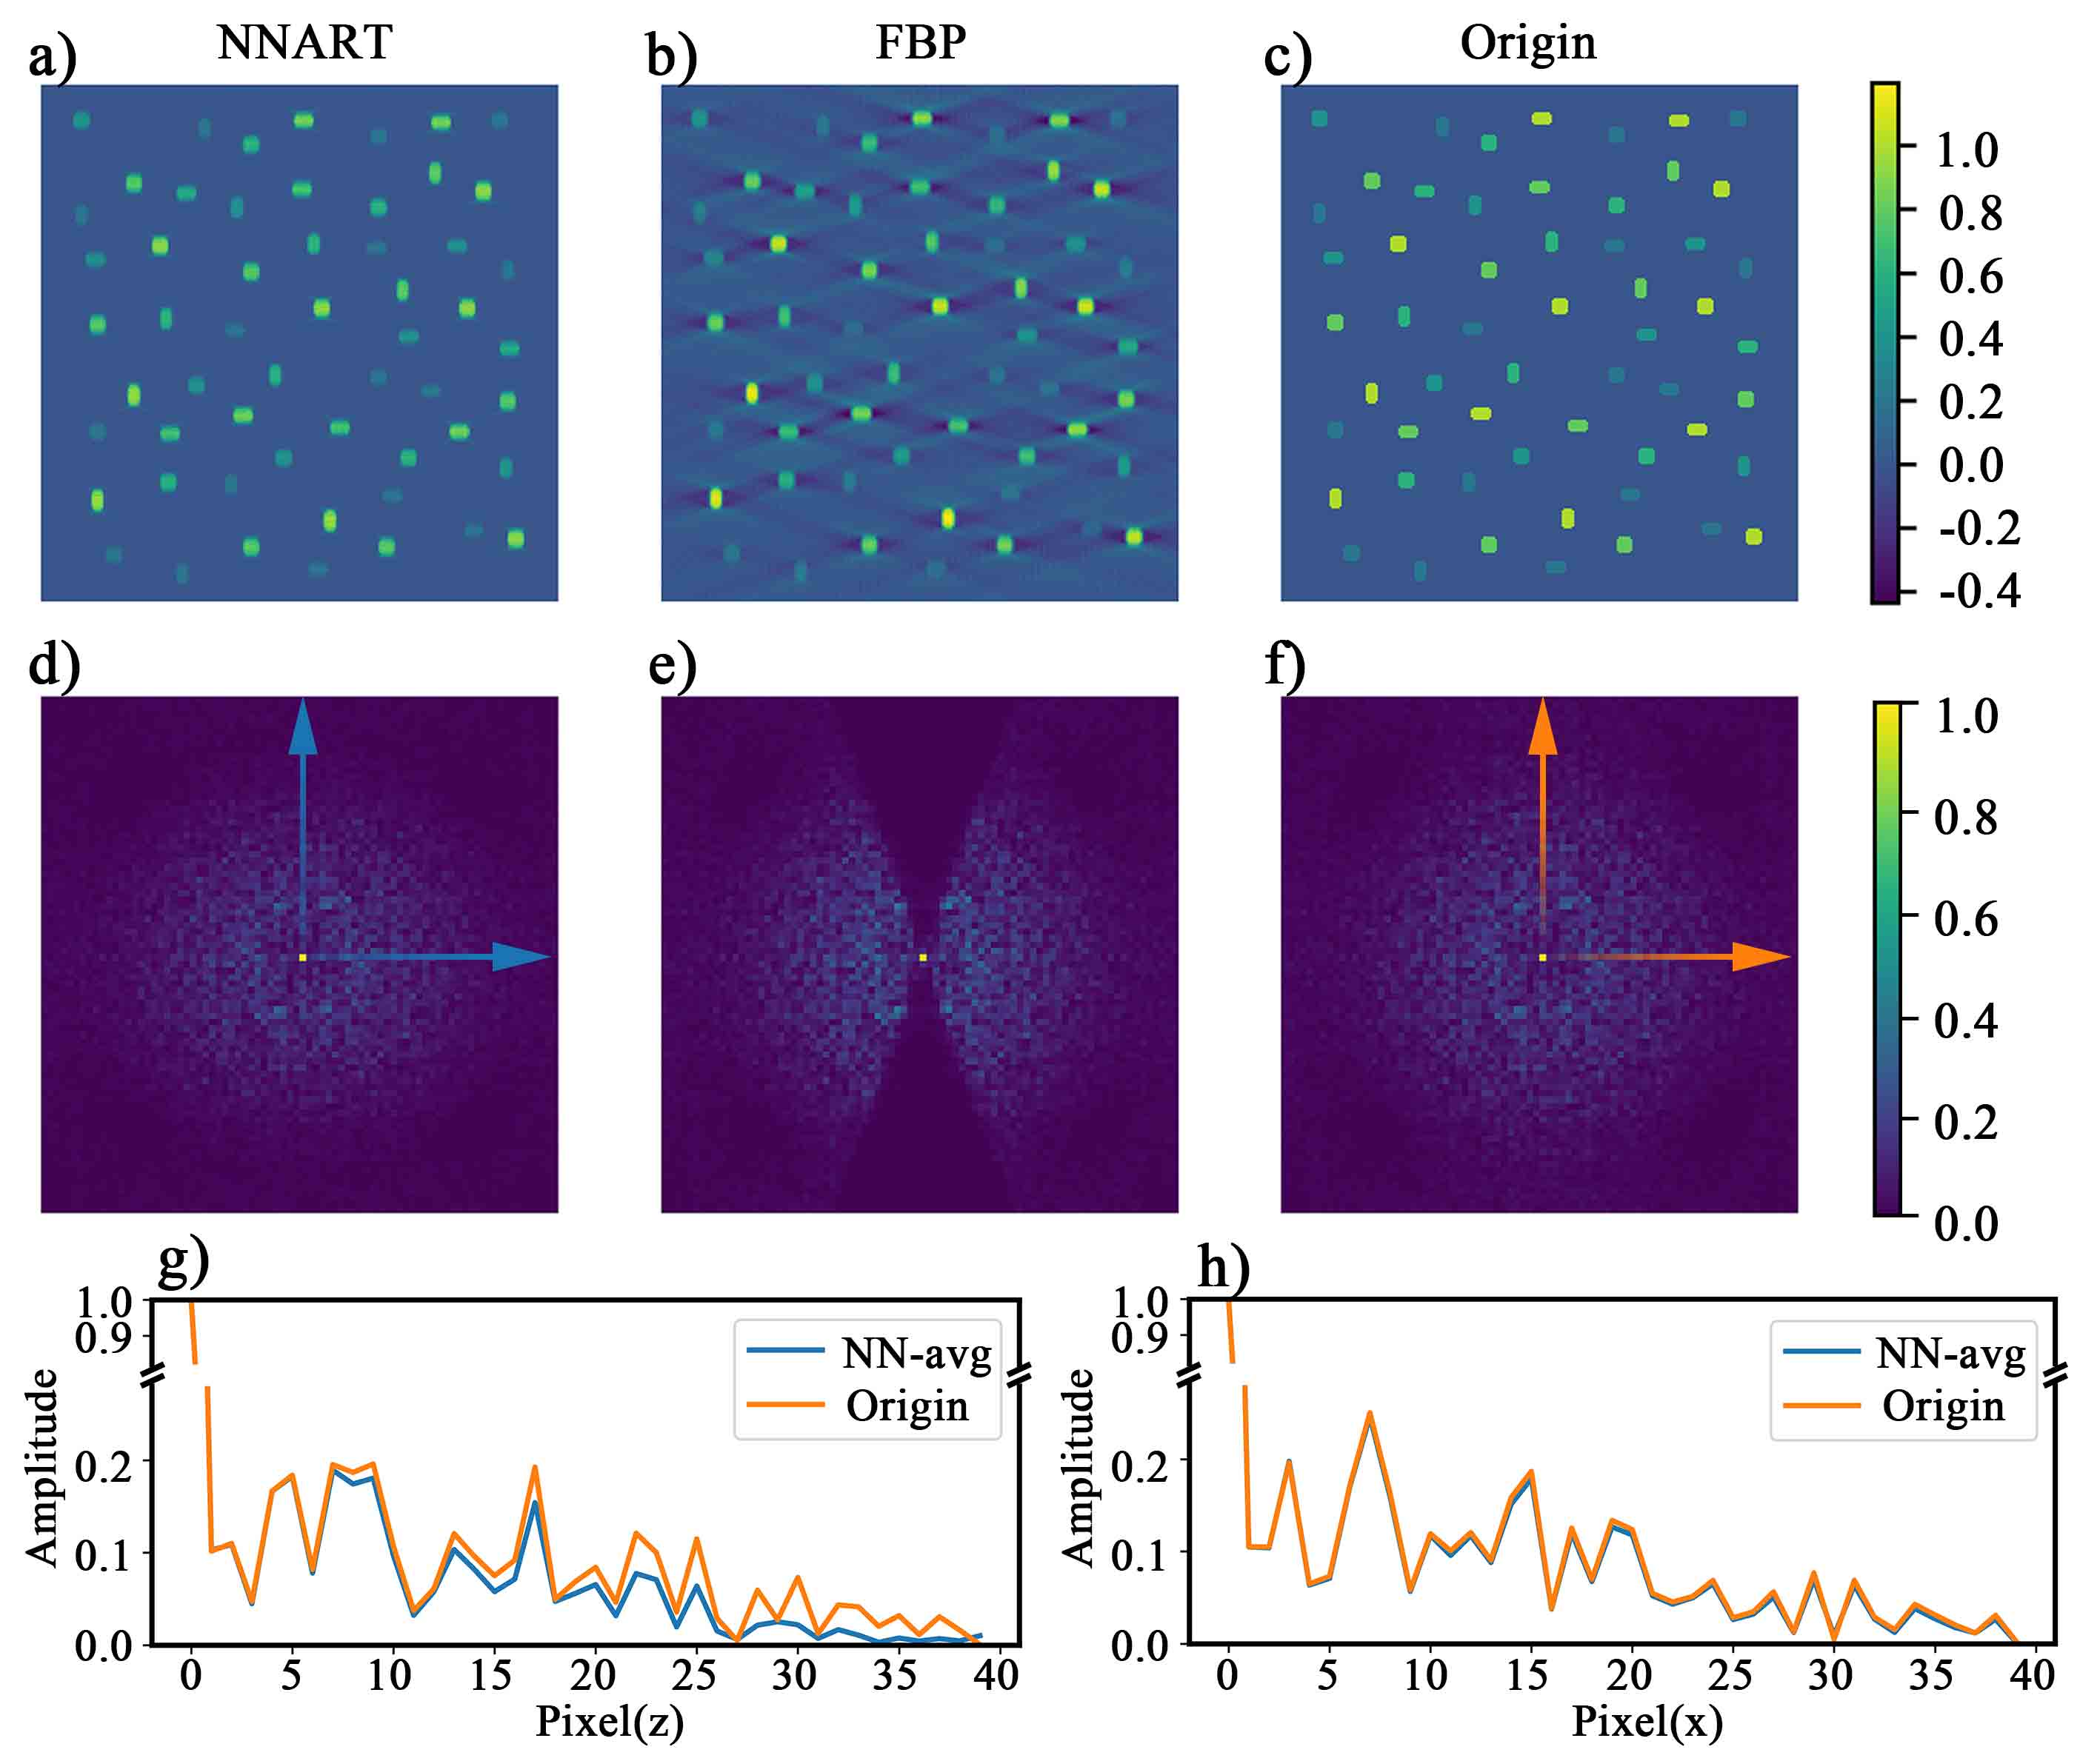
\includegraphics[width=0.9\textwidth]{../3.13/313}
	\caption{NNART 与 FBP 重构纳米颗粒模型的对比图}\label{fig:313}
	\song\tuzhu{a,b) NNART 和 FBP 重构纳米颗粒模型的结果;c) 纳米颗粒模型;d-f) a,b,c 的傅里叶变换;g,h) d 与 f图中沿 $z$ 轴和 $x$ 轴的强度对比图;重构的 sinogram 的倾转角范围是 -70° 到 +70°}
\end{figure}


本节还利用纳米颗粒模型,探究了极端情况下的重构情况。在 limited data 情形下,sinogram 的倾转角为 -70° 到 +70°,但间隔为 3°,投影数据缩减至原来的 1/3。此时,FBP 的重构结果(图 2.8b)中具有非常严重的条纹假象,在其傅里叶变换(图 2.8f)中也可明显地看出数据量的稀少(边缘出现条纹)。NNART 的重构结果的质量则高很多,没有出现条纹假象。而在 limited angle 情形下,sinogram 的倾转角为 -40° 到 +40°,间隔为 1°。此时 FBP 的重构结果中颗粒在 $z$ 方向上拉伸得特别明显,而 NNART 能够在一定程度上抑制这些假象,恢复出 $z$ 方向上的信息。从图 2.8i 的定量对比中可以看出,在两种情形下,缺失锥中的信息仍然被恢复出了一部分,尽管不如图 2.7g 中恢复的程度高。而在图 2.8j 中,可见在 limited data 情形下,即使在 $x$ 方向上,NNART 也无法完美恢复出频率信息,该结果符合预期。


\begin{figure}[H]
	\vspace{\baselineskip}
	\centering
	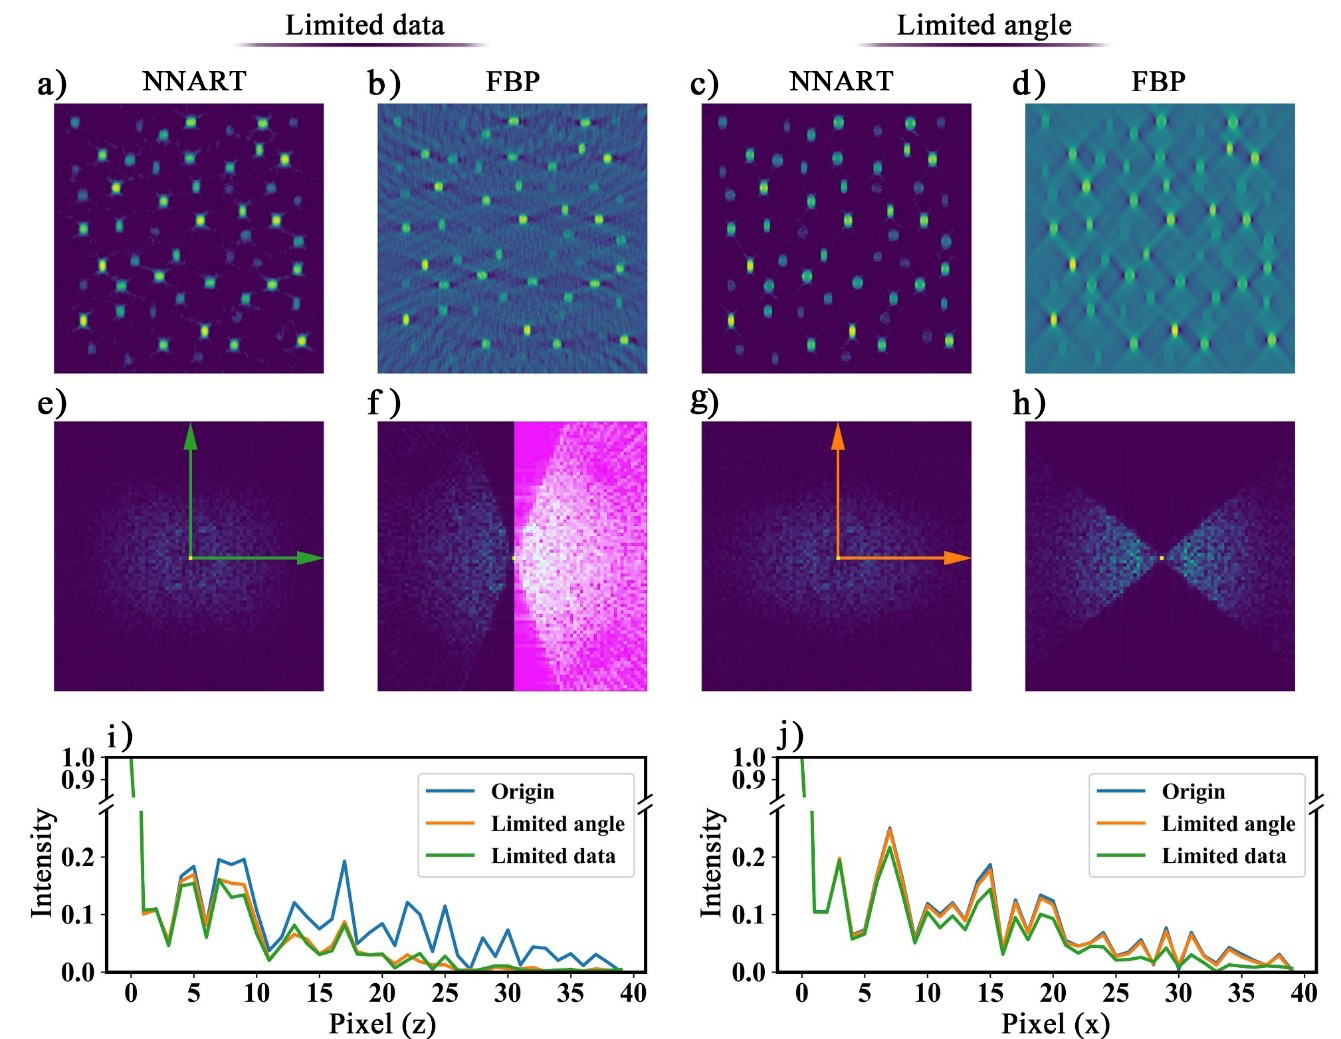
\includegraphics[width=0.9\textwidth]{../3.14/314}
	\caption{Limited data 和 limited angle 情形下纳米颗粒模型的重构结果对比}\label{fig:314}
	\song\tuzhu{a,b) Limited data 情形下 NNART 和 FBP 重构纳米颗粒模型的重构结果;c,d) Limited angle 情形下 NNART 和 FBP 重构纳米颗粒模型的重构结果;e-h) a,b,c,d 的傅里叶变换,f 右半边改变了图像衬度以更好地进行展示;i,j) e 和 g 与原始数据图 2.7f 中沿 $z$ 轴和 $x$ 轴的强度对比图;Limited data 情形下 sinogram 的倾转角为 -70° 到 70°,间隔为 3°;Limited angle 情形下的 sinogram 的倾转角为 -40° 到 40°,间隔为 1°}
\end{figure}

以上测试的模型中,强度都是分段不变的,下面以三个矩形模型为例,来探究当样品的成分分布具有梯度变化时 NNART 的重构效果。图 2.9d-f 是三个纵横比为 5 的矩形模型 rec1,rec2 和 rec3,其中 rec1 中的强度恒定,而 rec2 和 rec3 中的强度分别沿 $x$ 和 $z$ 轴呈梯度变化。在这种情况下,如图 2.9a-c 所示,在倾转角为 -70° 到 +70° 时,NNART 依然能够较好地重构矩形的整体形状,缺失锥假象被大幅抑制。不过,通过对比可见,图 2.9b 中矩形沿 $x$ 方向的强度变化在一定程度上被重构了出来,但是在图 2.9c 中则完全分辨不出强度是沿 $z$ 轴变化的。图 2.9g 和 h 是重构结果和原始模型的频率信息沿 $x$ 和 $z$ 轴的强度对比曲线。图 2.9g 证明 NNART 在重构 $x$ 方向的信息时是较为精确的。而在 2.9h 中,由于模型较大的纵横比,缺失锥范围内的信息在高频时较难被恢复,且当样品中的成分变化时,恢复的效果变差。正确重构物体的强度信息(成分)比重构物体的形状困难很多。特别地,当成分沿 $z$ 方向梯度变化时,这些频率信息将在缺失锥中丢失,更加难以复原。

\begin{figure}[H]
	\vspace{\baselineskip}
	\centering
	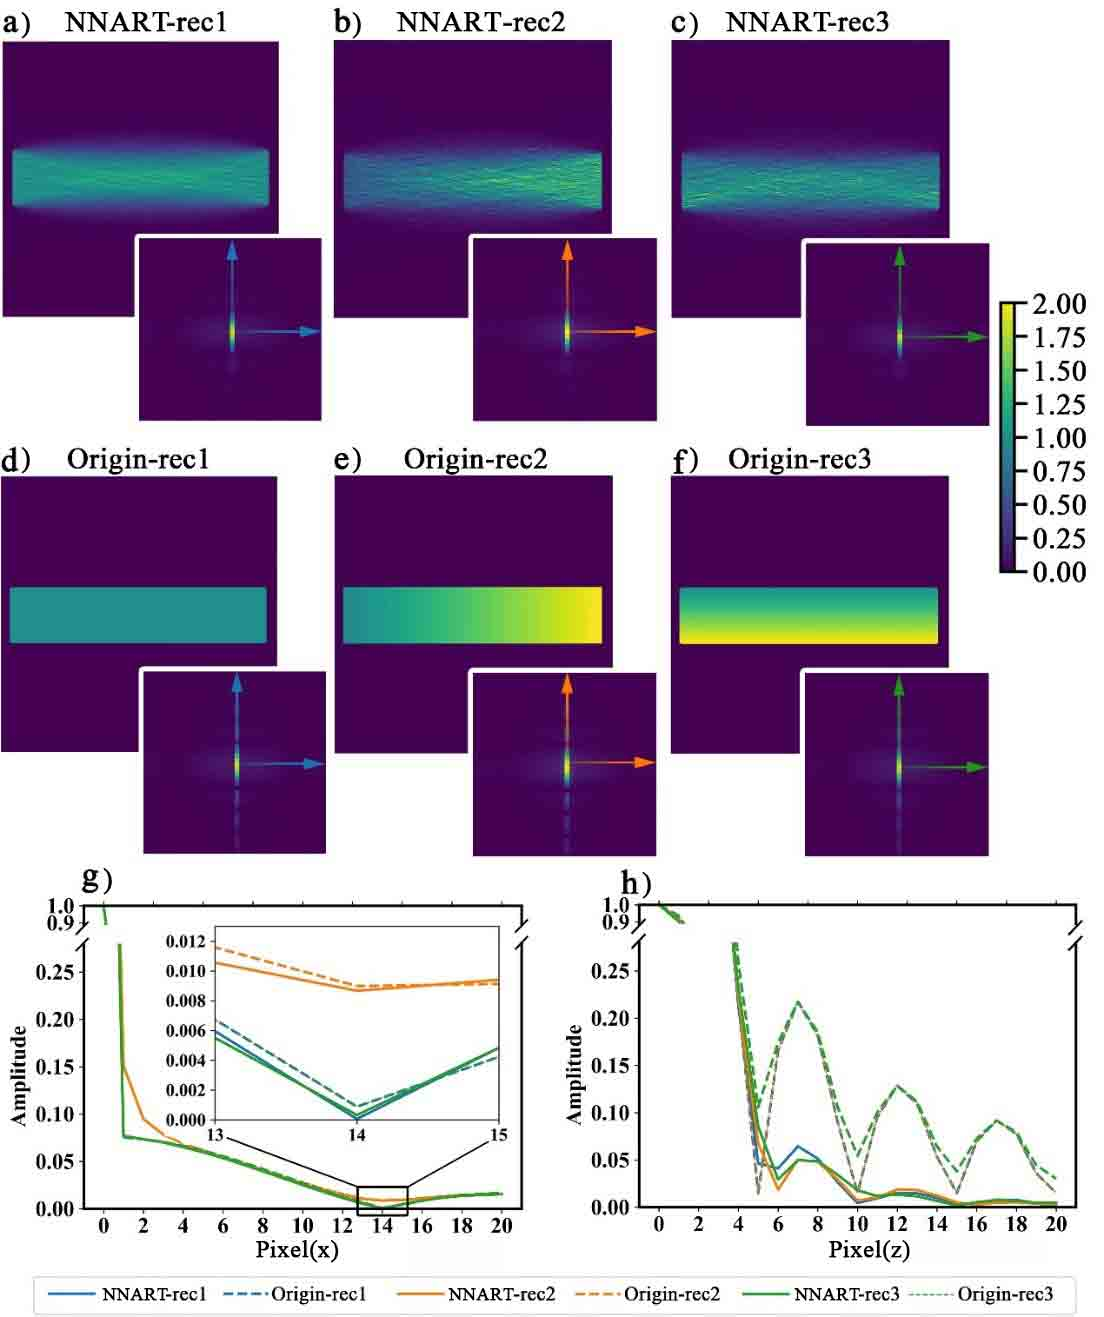
\includegraphics[width=0.9\textwidth]{../3.15/315}
	\caption{三个矩形模型与 NNART 的重构结果}\label{fig:314}
	\song\tuzhu{a-c) 纵横比为 5 的矩形模型 rec1,rec2 和 rec3 的 NNART 重构结果;d) 模型 rec1;e) 模型 rec2,强度沿 $x$ 方向梯度分布;f) 模型 rec3,强度沿 $z$ 方向梯度分布;g,h) 傅里叶空间中沿 $x$ 和 $z$ 轴的强度对比图;所有重构的倾转角范围是 -70° 到 +70°}
\end{figure}

另一个值得讨论的问题是,对于具有周期性的物体,其傅里叶空间的信息集中在固定的频率上。准确地恢复这些周期性的信息是检验 NNART 是否能抑制缺失锥假象和恢复缺失信息的一个很好的标准。图 2.10c 展示了一张模拟的 STEM 原子像,其中的原子在图像中周期性排列。它的傅里叶变换如图 2.10f 所示,其信息强度也是按周期性分布的。对该模型进行 -70° 至 +70° 的倾转投影得到带有缺失锥的 sinogram。图 2.10b 展示了使用 FBP 的重构结果,其中伸长假象和暗影假象非常明显。其傅里叶变换(图 2.10e)中 $z$ 轴上的信息完全缺失。而在 NNART 的重构结果(如图 2.10a 所示)中,原子的形状更接近圆形,暗影假象减弱很多。在它的傅里叶变换(图 2.10d)中,如红色箭头所示,缺失的信息被恢复。图 2.10g 和 h 定量对比了图 2.10d 和 f 沿 $x$ 和 $z$ 轴的强度,显然 NNART 完全恢复了沿 $x$ 轴的信息,而 $z$ 轴上的信息也在很大程度上被恢复出来,这说明 NNART 的确能够正确地恢复出缺失的信息。

\begin{figure}[H]
	\vspace{\baselineskip}
	\centering
	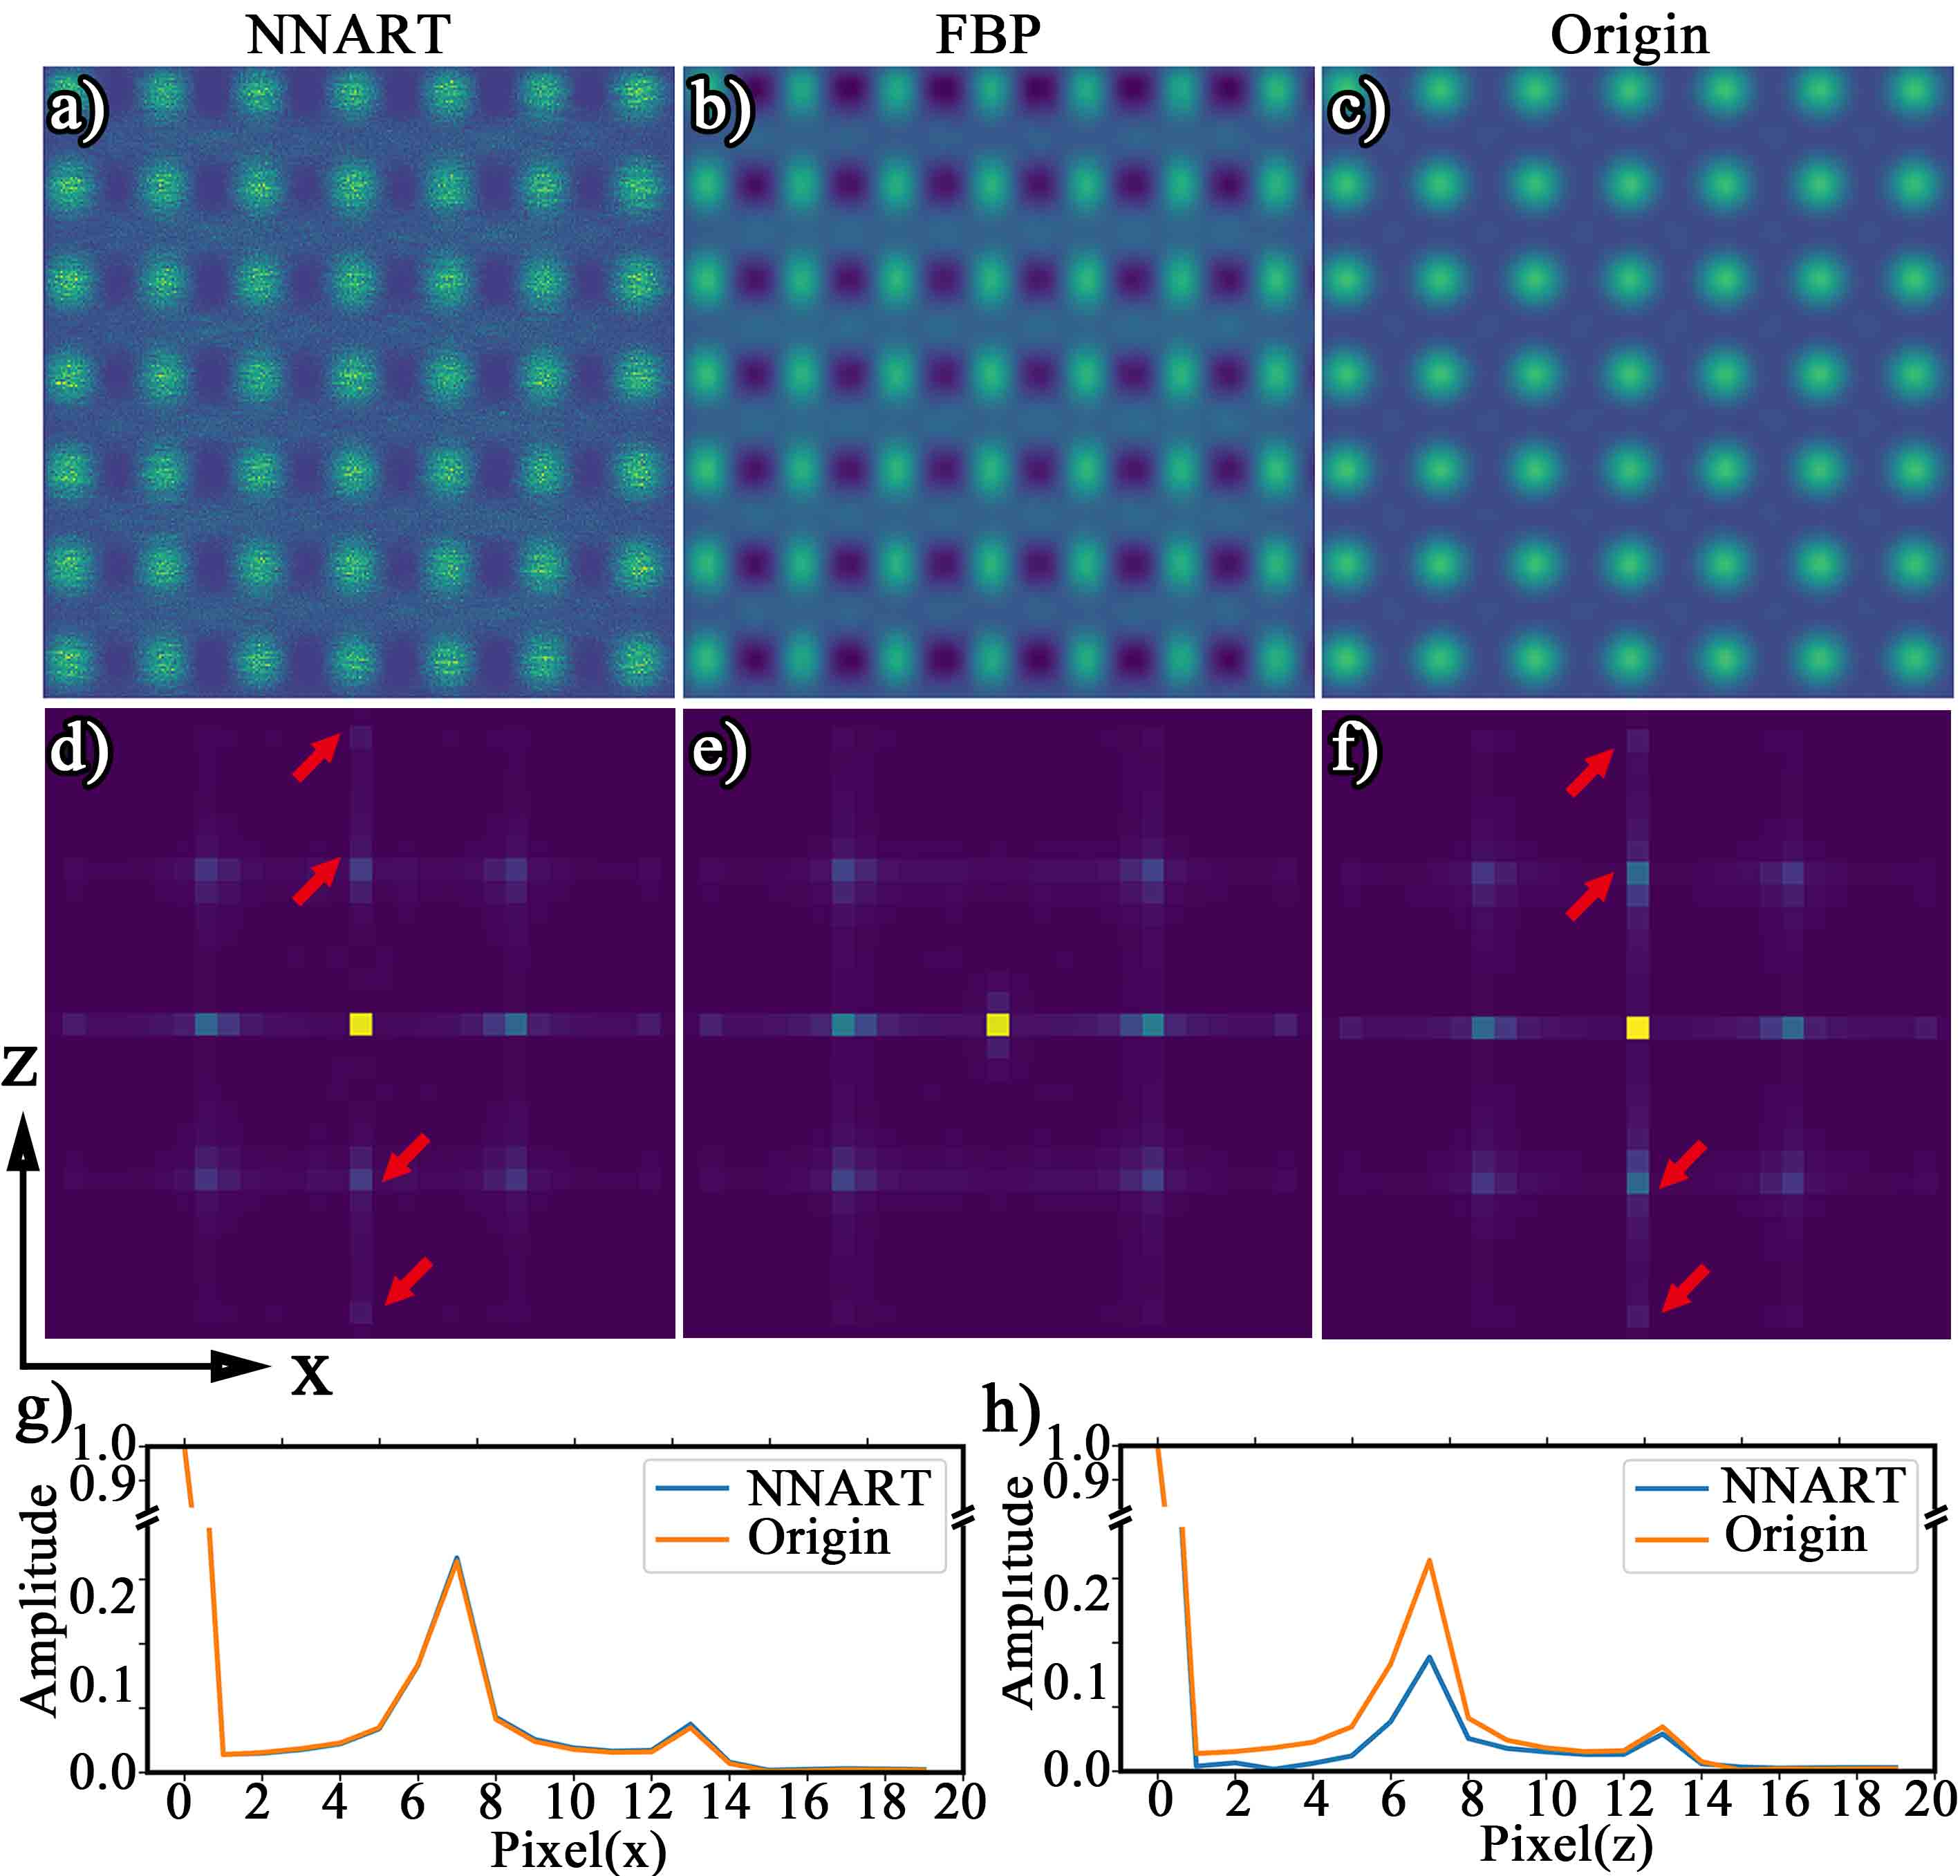
\includegraphics[width=0.9\textwidth]{../3.7/37}
	\caption{NNART 对 STEM 模拟原子像的重构测试}\label{fig:37}
	\song\tuzhu{a,b) NNART 和 FBP 重构 STEM 模拟原子像的带有缺失锥的 sinogram 的重构结果;c) STEM 模拟原子像;d,e,f) 图 a,b,c 的傅里叶变换(仅展示中间局部区域);g,h) 图 d 和 f 沿 $x$ 轴和 $z$ 轴的振幅对比曲线;sinogram 的倾转角范围是 -70° 至 +70°,倾转间隔是 1°}
\end{figure}

\section{实验及结果}
本节使用 NNART 重构了 SiC 样品,以验证 NNART 在实验数据中的适用性。SiC 样品是非晶转化法制备的纳米晶连续 SiC 纤维,制备工艺是将含铝的聚碳硅烷在 300 °C 的氮气保护下熔融纺丝、160  °C 空气中预氧化,随后在 1800 °C 氮气保护下热裂解。如图 2.11a 所示,样品是经离子束切割的 SiC 纤维的截面样品~\cite{Zhang2018},呈圆盘状且纵横比很大。样品在 FET Tecnai F20 透射电镜中,沿 $y$ 轴为倾转轴,以 -70° 至 +70°,1° 为间隔拍摄 HAADF-STEM 倾转系列像。本研究只重构了图 2.11a 中感兴趣区区域的部分。图 2.11b 展示了感兴趣区区域的倾转前(倾转角为 0°)的 HAADF-STEM 实验图像。其中石墨或游离炭由于 C 元素的原子序数很小,所以在 HAADF-STEM 像中呈暗衬度,如白色箭头所示。可见,这些石墨或游离碳没有固定的形状,它们不规则地分布在 SiC 基体中,形成了复杂的内部形貌。当样品倾转至 70° 时,可从图 2.11c 和 b 的对比看出,其 HAADF-STEM 的图像强度明显增强,这是因为在大倾转角下,样品沿 $z$ 轴的有效厚度增大导致的。图 2.11c 中最右侧的亮衬度物质是离子束切割过程中,样品表面沉积的重元素 Pt。另可知图 2.11b 所展示的感兴趣区,在图 2.11c 中仅为两条红色虚线内的区域。最后,在进行三维重构之前,所有的 141 张倾转系列 HAADF-STEM 图像都使用了互相关法进行了漂移矫正。

\begin{figure}[htbp]
	\vspace{\baselineskip}
	\centering
	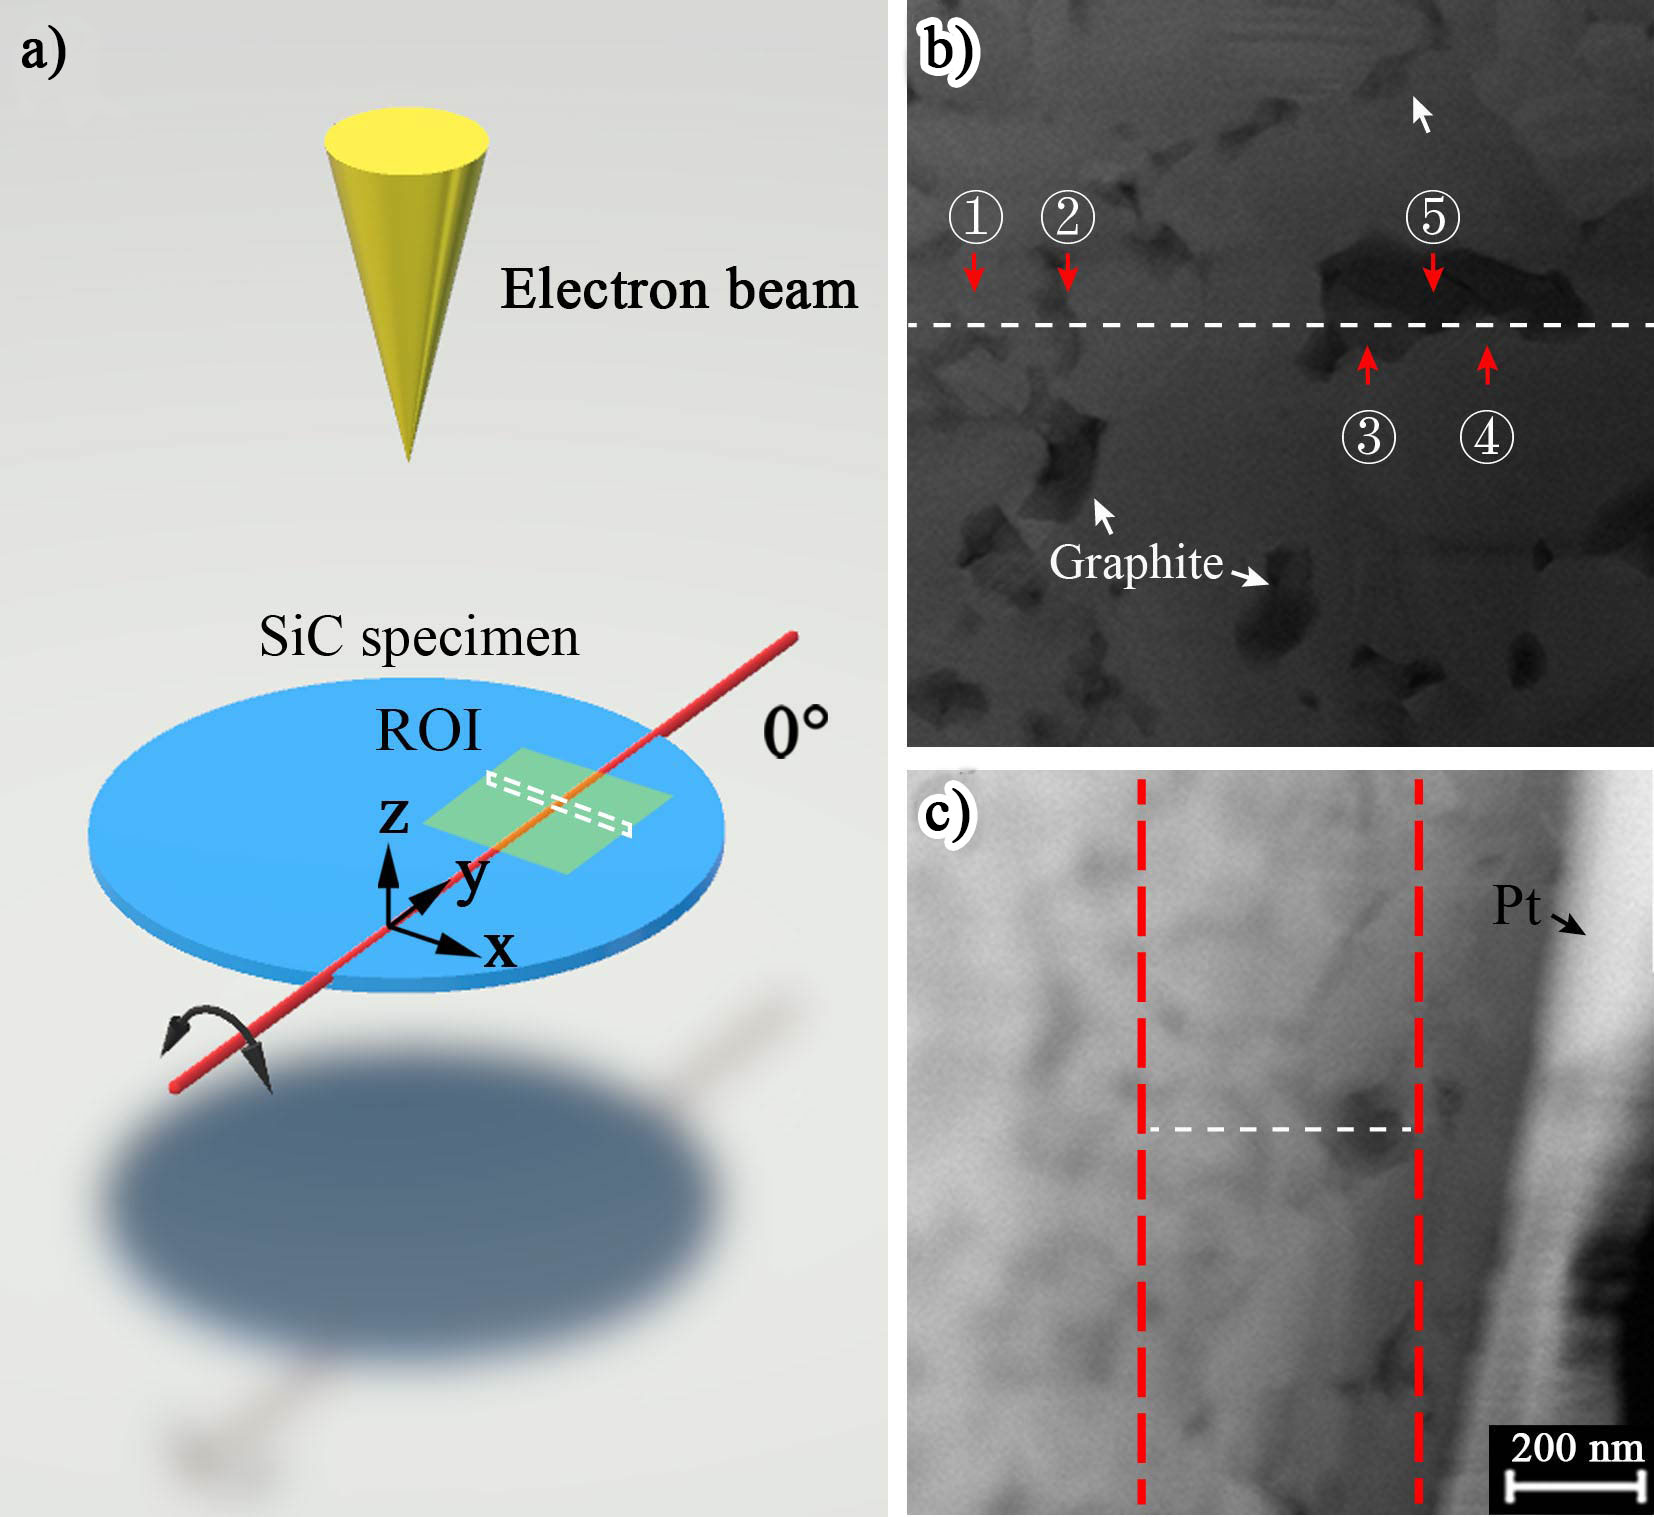
\includegraphics[width=0.9\textwidth]{../3.8/38}
	\caption{SiC 样品图示}\label{fig:38}
	\song\tuzhu{a) SiC 样品在 HAADF-STEM 倾转系列像实验中的布局示意图,电子入射方向沿z轴向下;b, c)SiC 分别倾转 0°(倾转前)和倾转 70° 时的 HAADF-STEM 实验像;图 b 的视野是感兴趣区,而其仅为图 c 中两条红色虚线之间的区域;图 a 中的白色虚线框和图 b 与 c 中的白色虚线表示了样品中某一片层,图 b 中标注的 5 个特征点有助于对重构结果的分析}
\end{figure}



 图 2.12a 和 c 展示了 NNART 和 TVM 重构的图 2.11b 中白色虚线处的一层 SiC 样品。图 2.12b 和 d 展示了图 2.12a 和 c 的傅里叶变换,显然 NNART 在傅里叶空间中恢复出了更多的缺失锥区域的信息,而 TVM\begin{figure}[b!]
 	\vspace{\baselineskip}
 	\centering
 	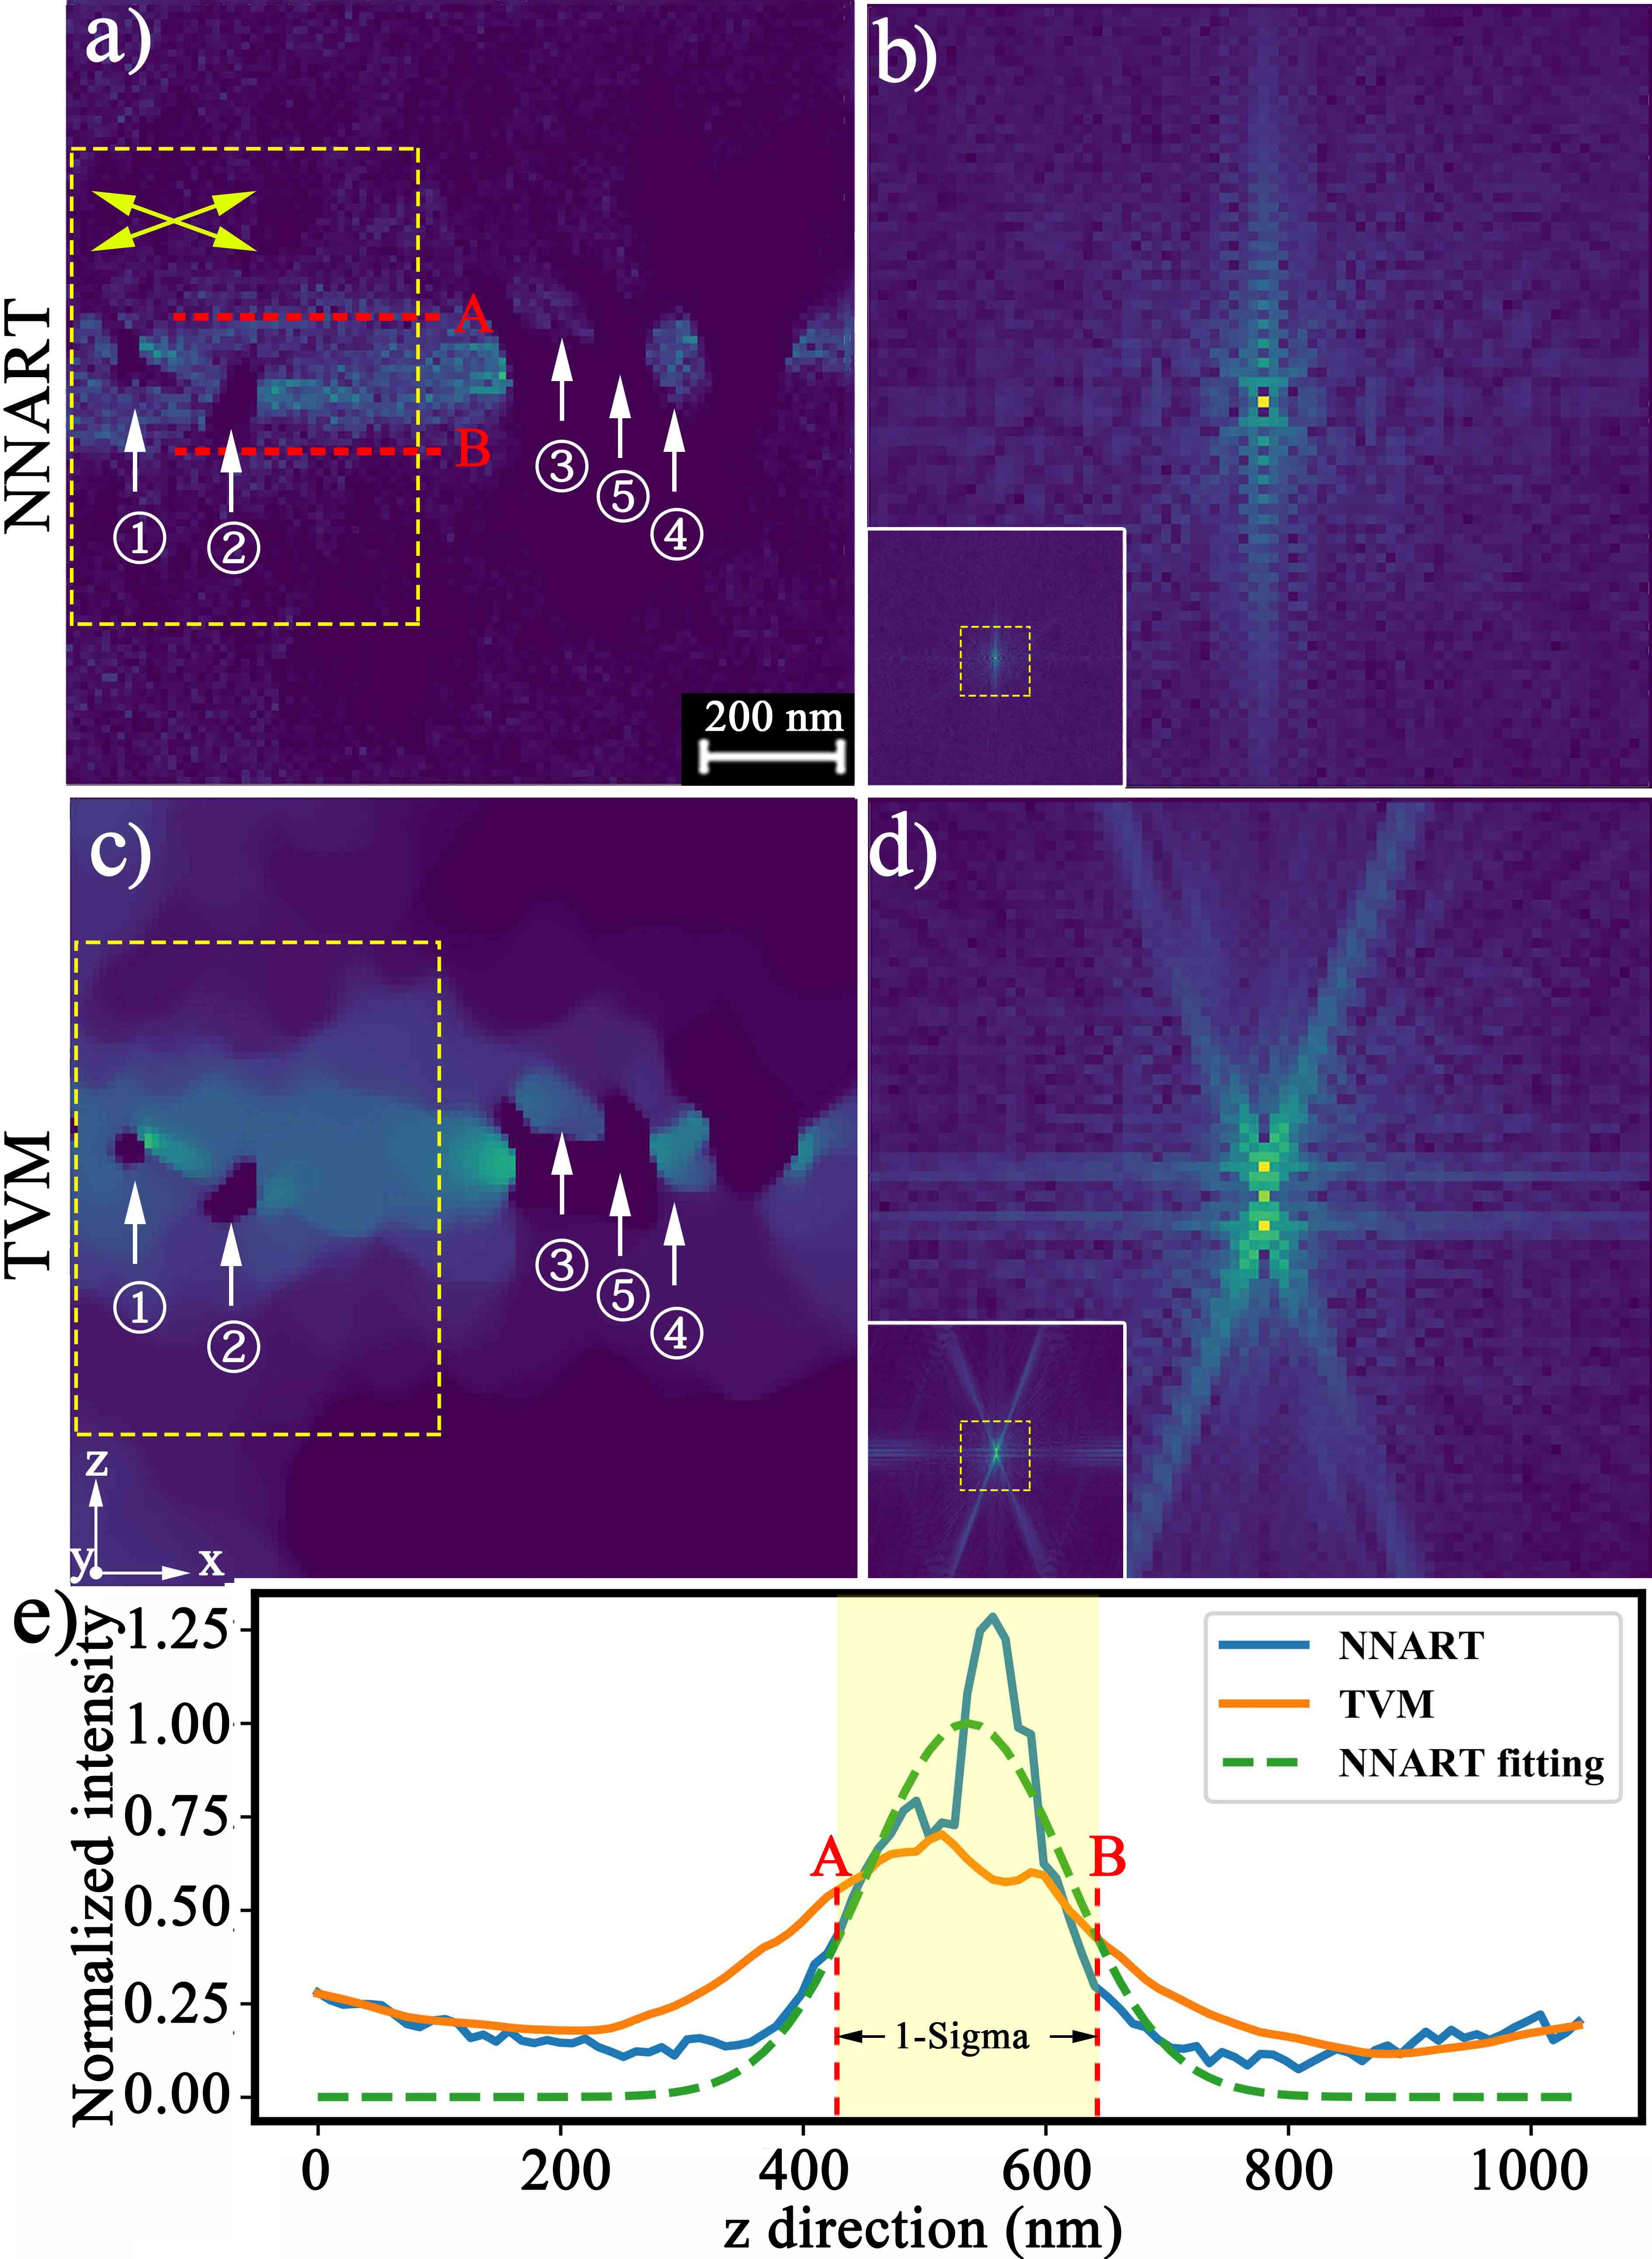
\includegraphics[width=0.65\textwidth]{../3.9/39}
 	\caption{NNART 和 TVM 重构的二维结果的对比}\label{fig:39}
 	\song\tuzhu{a, c) NNART 和 TVM 重构的图 2.8b 中白色虚线处的 SiC 样品,对应的 5 个特征同样用虚线标注;b, d) 图 a 和 c 的傅里叶变换(插入的小图)的中间放大图像;e) 图 a 和 c 中黄色虚线框中沿 $z$ 方向的归一化强度分布对比图,绿色虚线是蓝色实现的正态分布拟合曲线,其中红色虚线 A 和 B 与图 a 中的虚线位置对应,其中包括的是正态分布曲线的 1-Sigma 区域}
 \end{figure}仅在非常低频的位置恢复出了些许信息,整个信息缺失的锥形样貌在图 2.12d 中仍然非常明显。在这个实验案例中,TVM 对缺失信息的恢复比第 2.3 节中的模拟案例差很多,其原因是 TVM 将样品周围的噪音错误地加强了,这在图 2.12c 中表现得很明显。因此,TVM 重构的结果中的样品并不像离子束切割样品预期的那样边界笔直,很多被错误加强和平滑的噪音在其周围形成了不规则的形貌。而图 2.12a 中展现出的整体的样品形貌更加合理,尽管 NNART 无法去除来自实验数据的噪音。在两个算法的重构结果中,图 2.11b 中的特征 1、2、3、4 均得到了较为正确的还原,唯一不同的是图 2.11a 和 c 中恢复的特征 1 的形状并不相同,NNART 的重构结果是 $\lambda$ 形,这个结果经图 2.16i 和 j 可以验证,是正确的。而 TVM 的重构结果是一个小圆形,这是图像平滑处理的结果。所以 NNART 重构出了样品的更多细节。图 2.12e 是图 2.12a 和 c 中黄色虚线框中的图像强度沿 $z$ 方向的平均变化曲线。绿色的虚线是 NNART 测得的曲线的高斯分布拟合,其 1-Sigma 区域对应于图 2.12a 的 A、B 虚线,可见这是对样品厚度的合理测量。而 TVM 的曲线则宽很多,显然无法正确测量样品的厚度。
 
\begin{figure}[H]
	\vspace{\baselineskip}
	\centering
	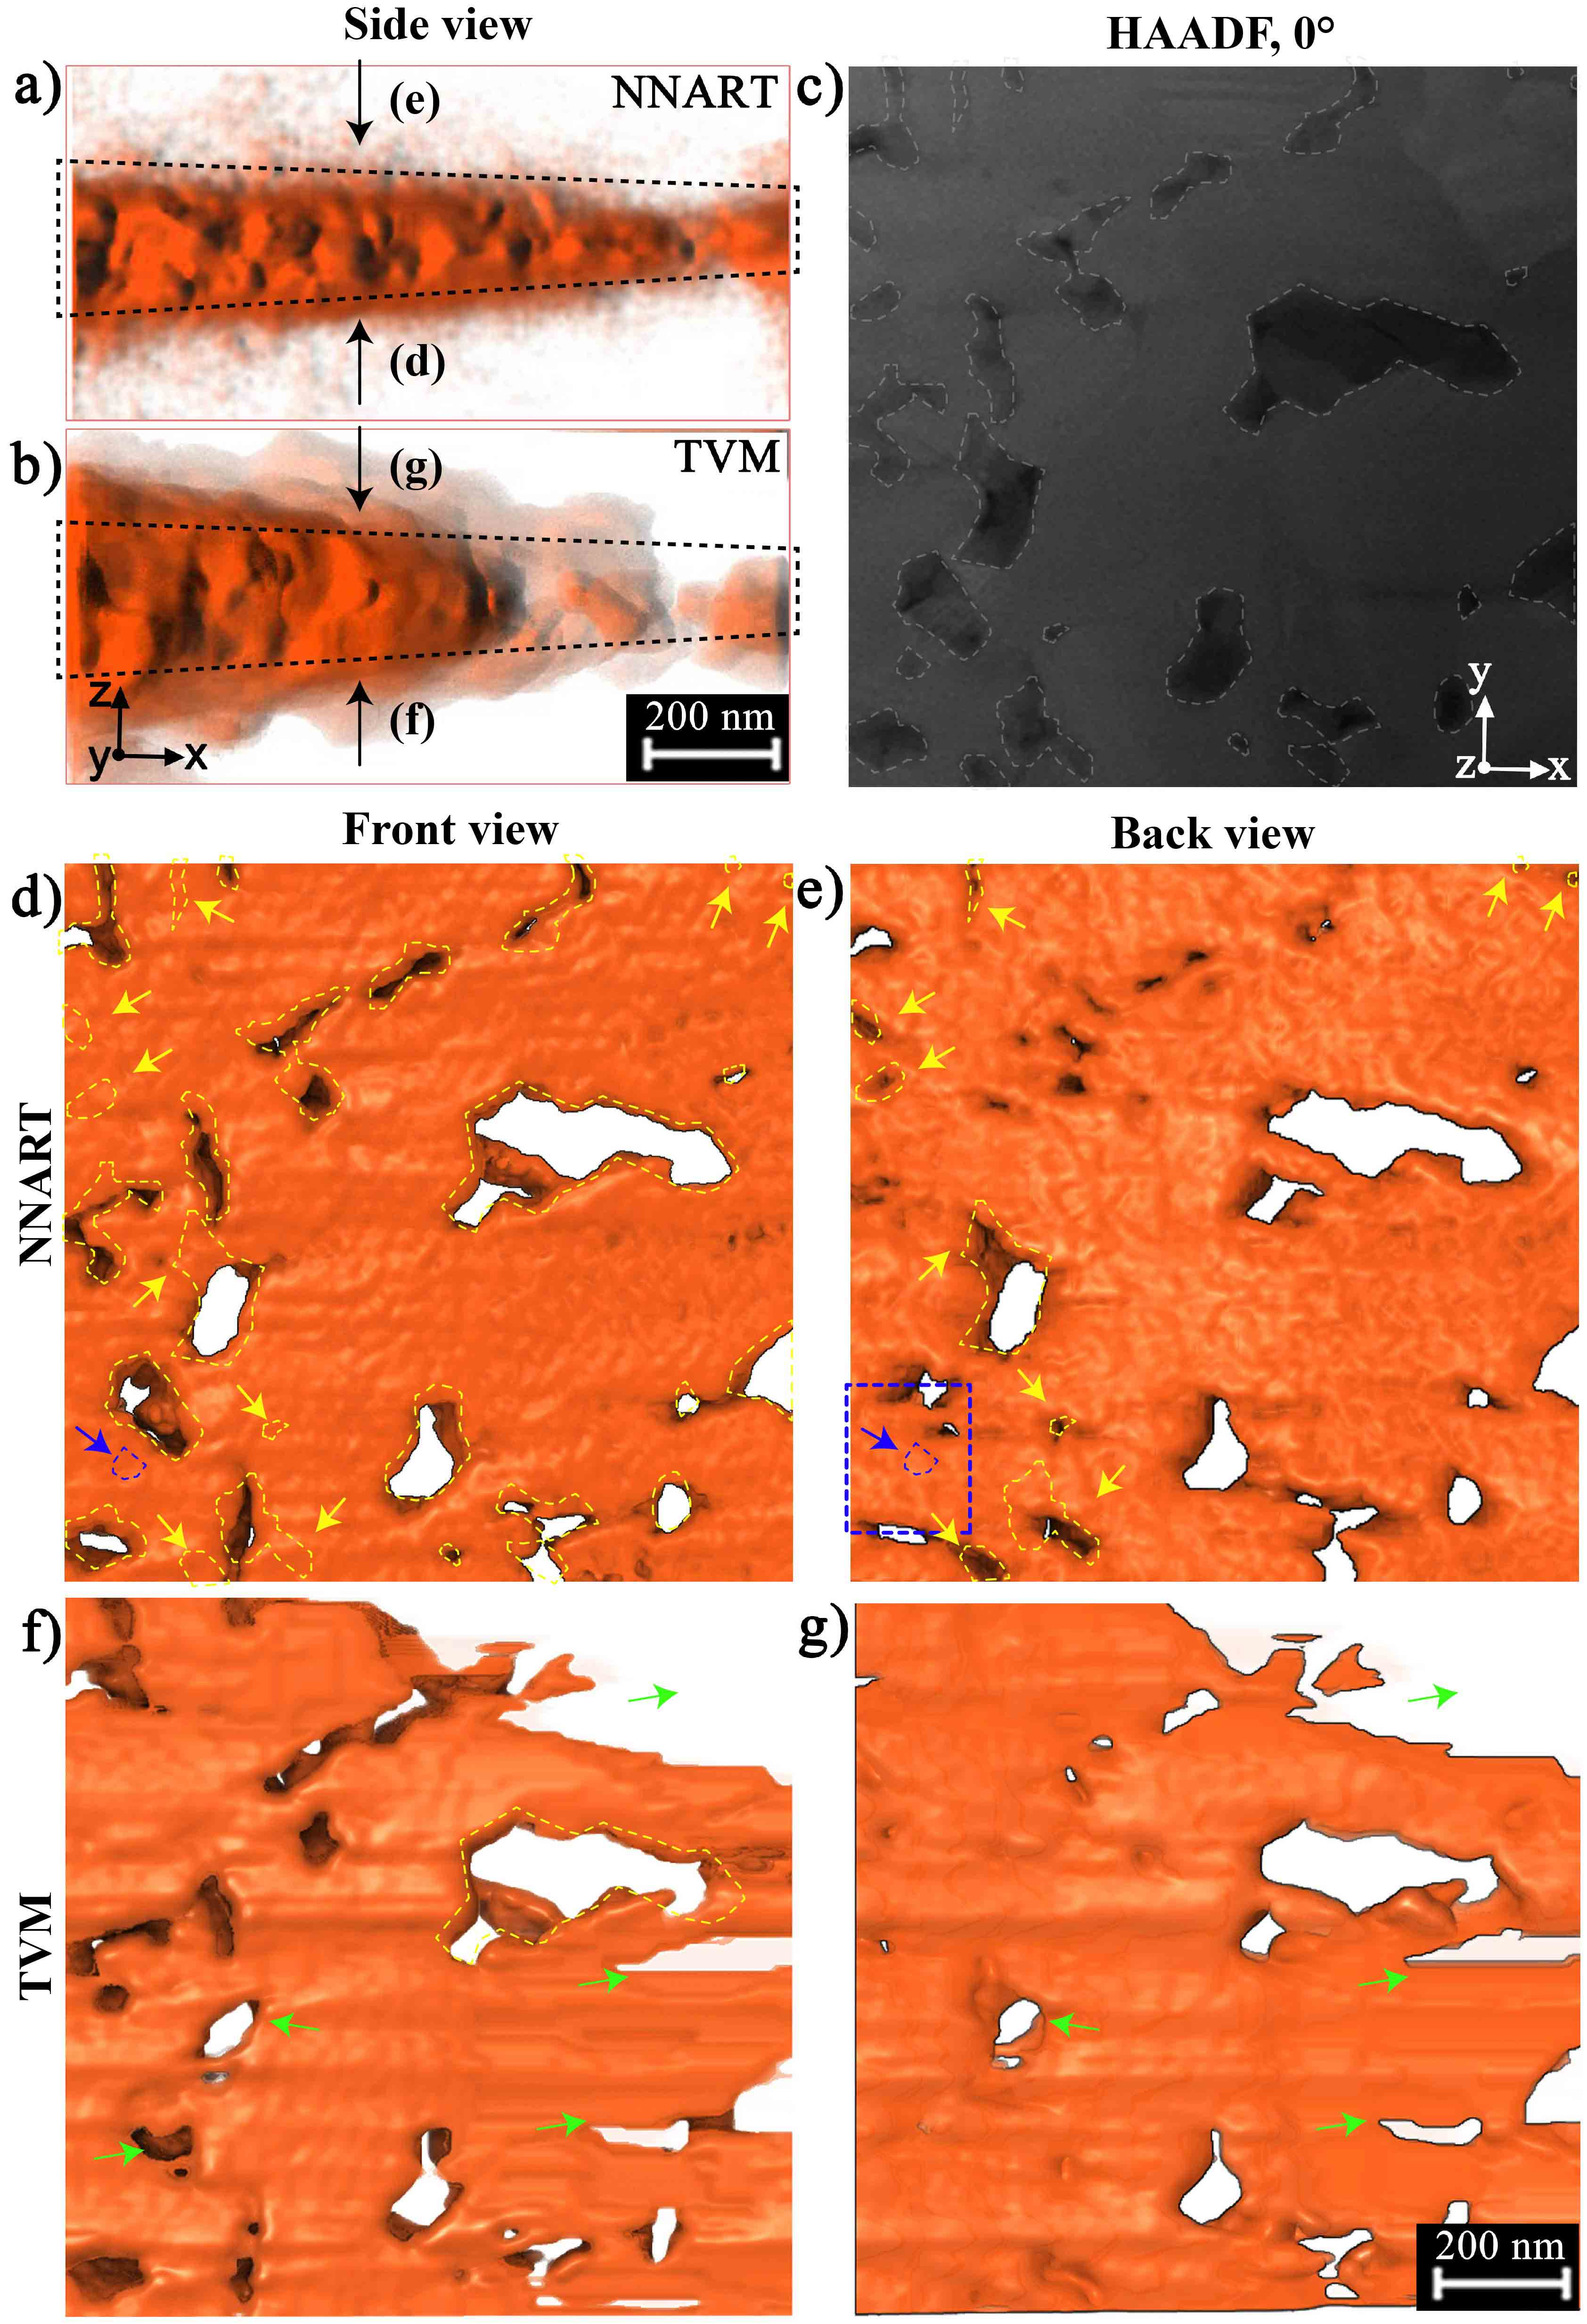
\includegraphics[width=0.65\textwidth]{../3.16/316}
	\caption{SiC 样品三维重构渲染图}\label{fig:310}
	\song\tuzhu{a,b) NNART 和 TVM 重构的 SiC 样品的俯视视角三维渲染图;c) 倾转角为 0° 时的  HAADF-STEM 实验图;d,e) 图 a 中虚线框内的重构结果的前视图和后视图;其中,图 d 中的虚线轮廓与图 c 中的一一对应,黄色箭头指出的形貌仅显示在图 e 中;蓝色虚线框处被剖开后可观察到蓝色箭头所指的相;f,g) 图 b 中虚线框内的重构结果的前视图和后视图;绿色箭头所指的形貌明显偏离图 c}
\end{figure}

图 2.13a 和 b 展示了 NNART 和 TVM 重构的 SiC 样品的三维渲染结果的俯视图(与图 2.12a 和 b 相同视角)。图 2.13a 清晰地展示出了一个具有厚度梯度的片状(离子束切割)样品的形貌,纵横比约等于 5。而图 2.13b 中 TVM 重构的结果并不理想,样品呈现出许多不规则的形貌,不符合离子束切割样品的形貌。为了进一步观察重构的样品的形貌,图 2.13d 和 e 展示了图 2.13a 中虚线框内部分的前视图和后视图。图 2.13c 和 d 中的虚线轮廓是一一对应的,通过对比可见石墨和游离碳相由于衬度较弱,显示为孔洞状,且图 2.13d 中能够观察到绝大部分的石墨和游离碳,形貌与实验图像吻合。少部分黄色箭头所指的相,在前视图中无法观察到,因为它们实际存在于背面,可在图 2.13e 中观察到。蓝色箭头与轮廓所指的相,存在于基体的内部,在图 2.13d 和 e 中均无法观察到。图 2.14 展示了将图 2.13e 中蓝色虚线框内的部分剖开后,不同深度处的样品形貌,可见该相存在于 $z \approx 65 \sim 135$ nm 的深度内。图 2.13f 和 g 展示的是图 2.13b 中虚线框内部分的前视图与后视图。可见,TVM 重构的形貌与实验图像相去甚远,仅黄色虚线轮廓中的大的石墨相得到了较好的重构,绿色箭头处还出现了严重的错误。综上可知,NNART 在重构该 SiC 样品时,具有非常大的优势,它的重构结果较为准确。






\begin{figure}[htbp]
	\vspace{\baselineskip}
	\centering
	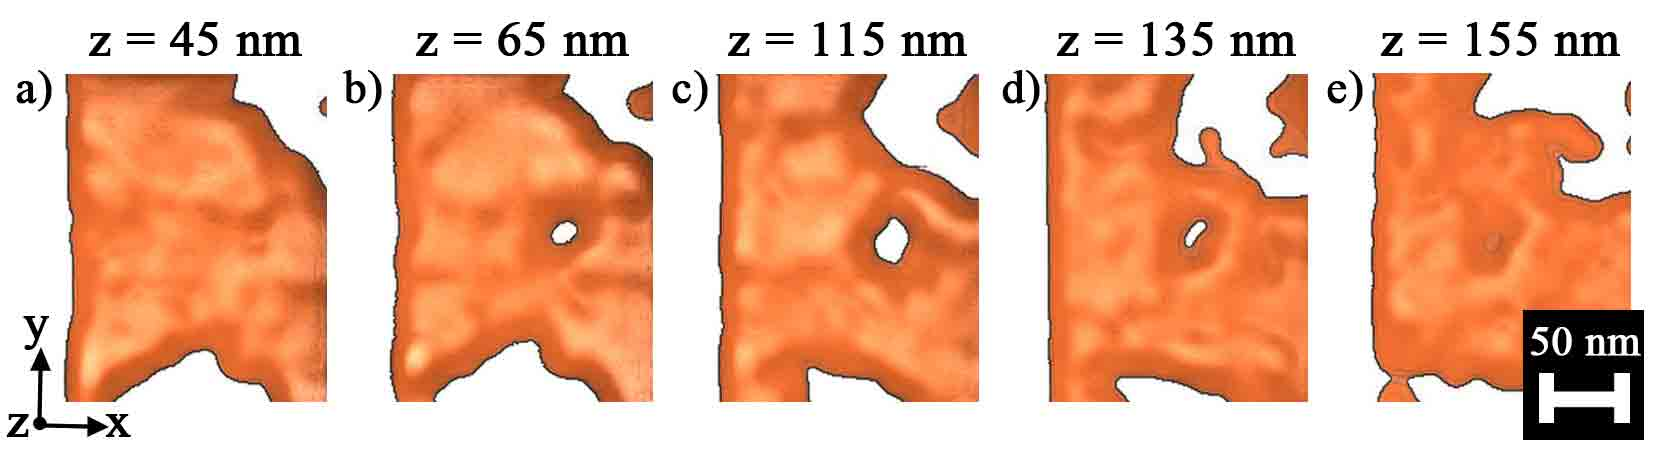
\includegraphics[width=0.9\textwidth]{../3.18/318}
	\caption{SiC 样品三维重构局部的切片渲染图}\label{fig:310}
	\song\tuzhu{a-e) 图 2.13e 中蓝色虚线框中部分在不同深度下的切片的渲染图,深度 $z$ 分别为 45、65、115、135 和 155 nm}
\end{figure}

为了进一步在三维的维度上说明 NNART 重构的样品形貌的准确性,图 2.15 对比了不同倾转角下的石墨相的的三维重构渲染图与实验图。可见在任意角度下,石墨相的三维渲染图展示的形貌与实验图像都非常相近,这说明这个石墨相的三维形貌被准确地重构了出来。由此可知 NNART 重构的样品形貌是相当准确的。
\begin{figure}[htbp]
	\vspace{\baselineskip}
	\centering
	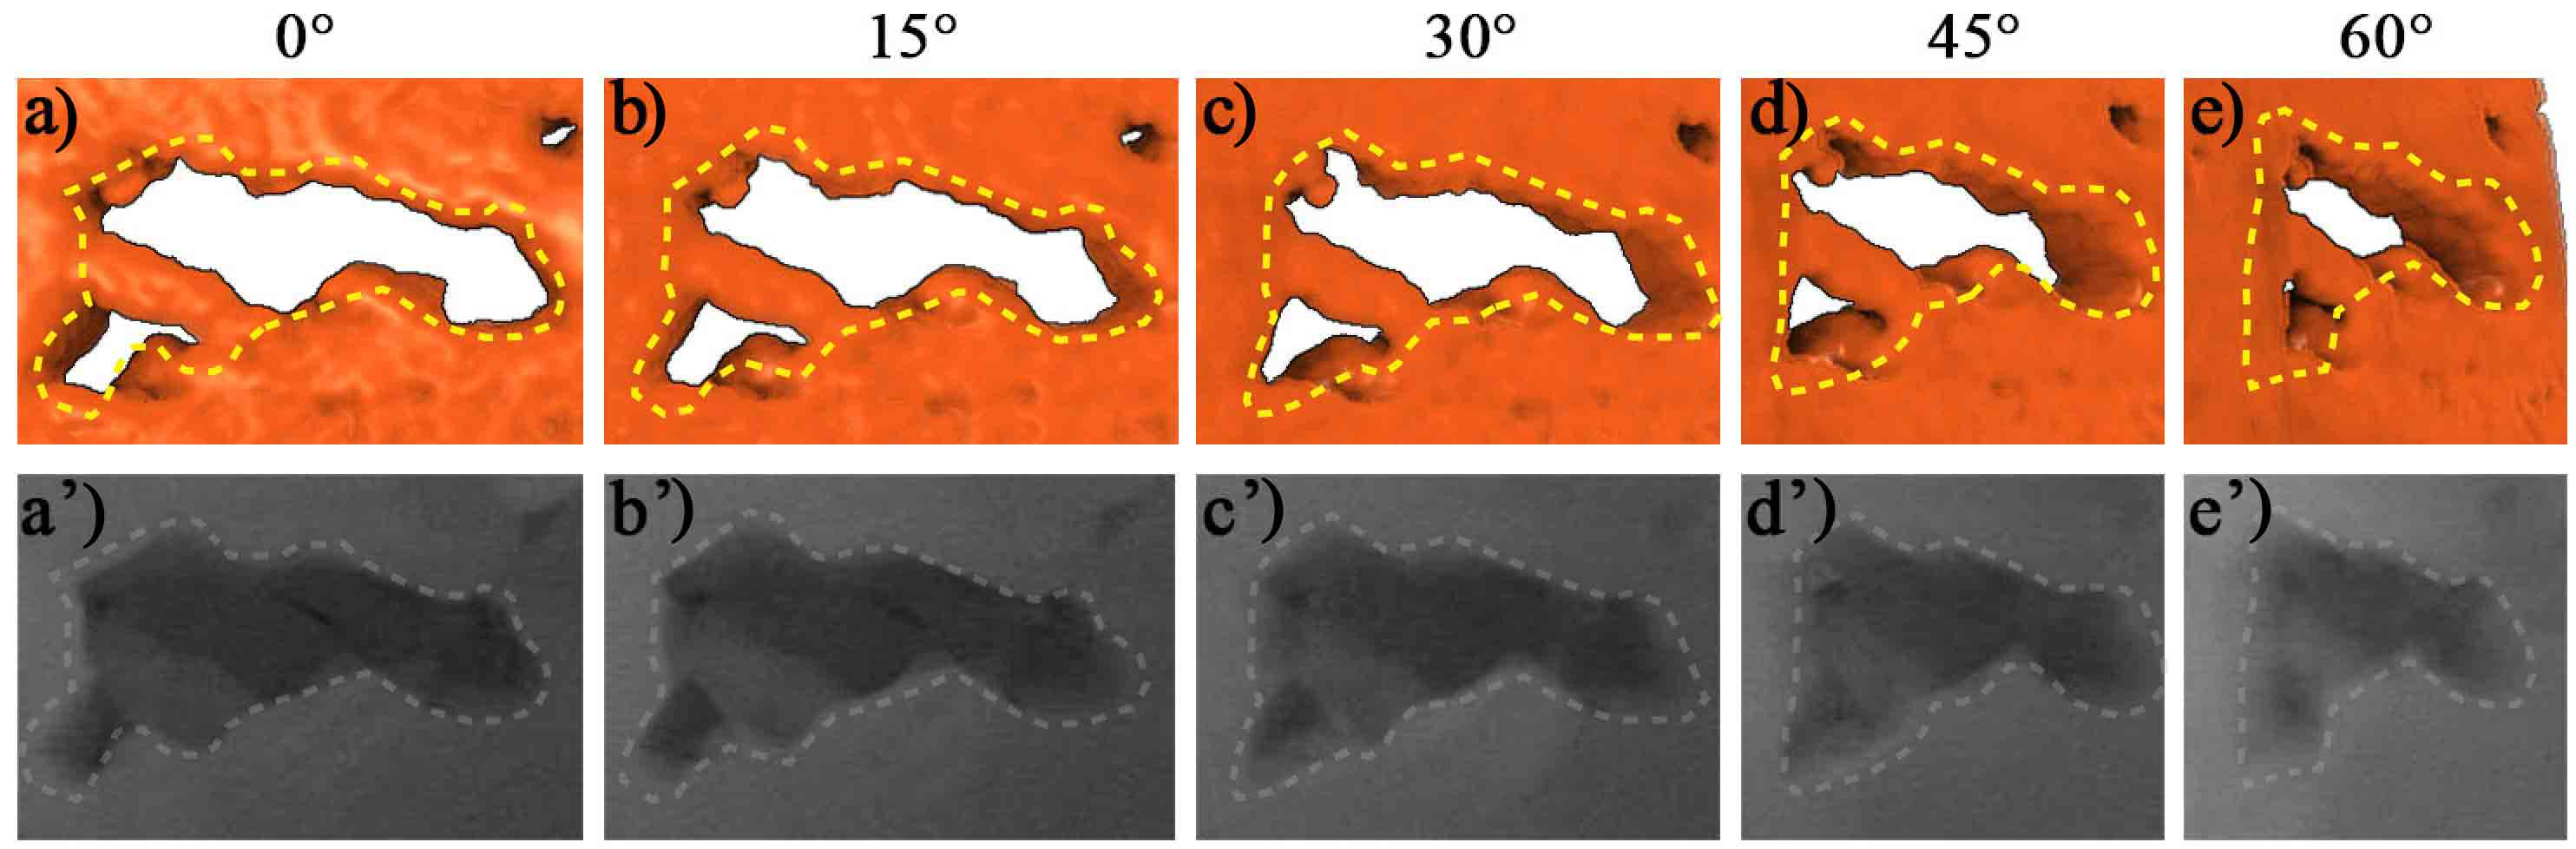
\includegraphics[width=0.9\textwidth]{../3.17/317}
	\caption{石墨相在不同倾转角下的三维渲染图与实验图像的对比}\label{fig:310}
	\song\tuzhu{a-e) NNART 重构的石墨相分别在 0°,15°,30°,45°,60° 倾转角下的三维渲染图;a'-e')  0°,15°,30°,45°,60° 倾转角下的石墨相的实验图}
\end{figure}

\section{NNART 与正则化}
本节将探究 NNART 的正则化,具体实施方法为在公式(2.6)的损失 $L$ 中加上一个正则化项:
\begin{equation}
L = \sum {\sqrt{|\boldsymbol{S}-\boldsymbol{S}^{exp}|}}+\alpha V
\end{equation}
其中 $\alpha$ 是正则化系数,$V$ 是正则化项。由于正则化的算法可以得到平滑解,所以在此不再需要使用“多次平均”,正则化后的 NNART 每次只需重构一次即可得到重构结果。研究中使用的正则化方法有 L2 范数、最大熵(香农熵)以及 TVM,其中 L2 和香农熵的正则化项分别为:
\begin{equation}
V_{\text{L2}} = \sum \boldsymbol{I}^2
\end{equation}
\begin{equation}
V_{\text{Shannon}} = -\sum \boldsymbol{I} \log_2 \boldsymbol{I}
\end{equation}

\begin{figure}[htbp]
	\vspace{\baselineskip}
	\centering
	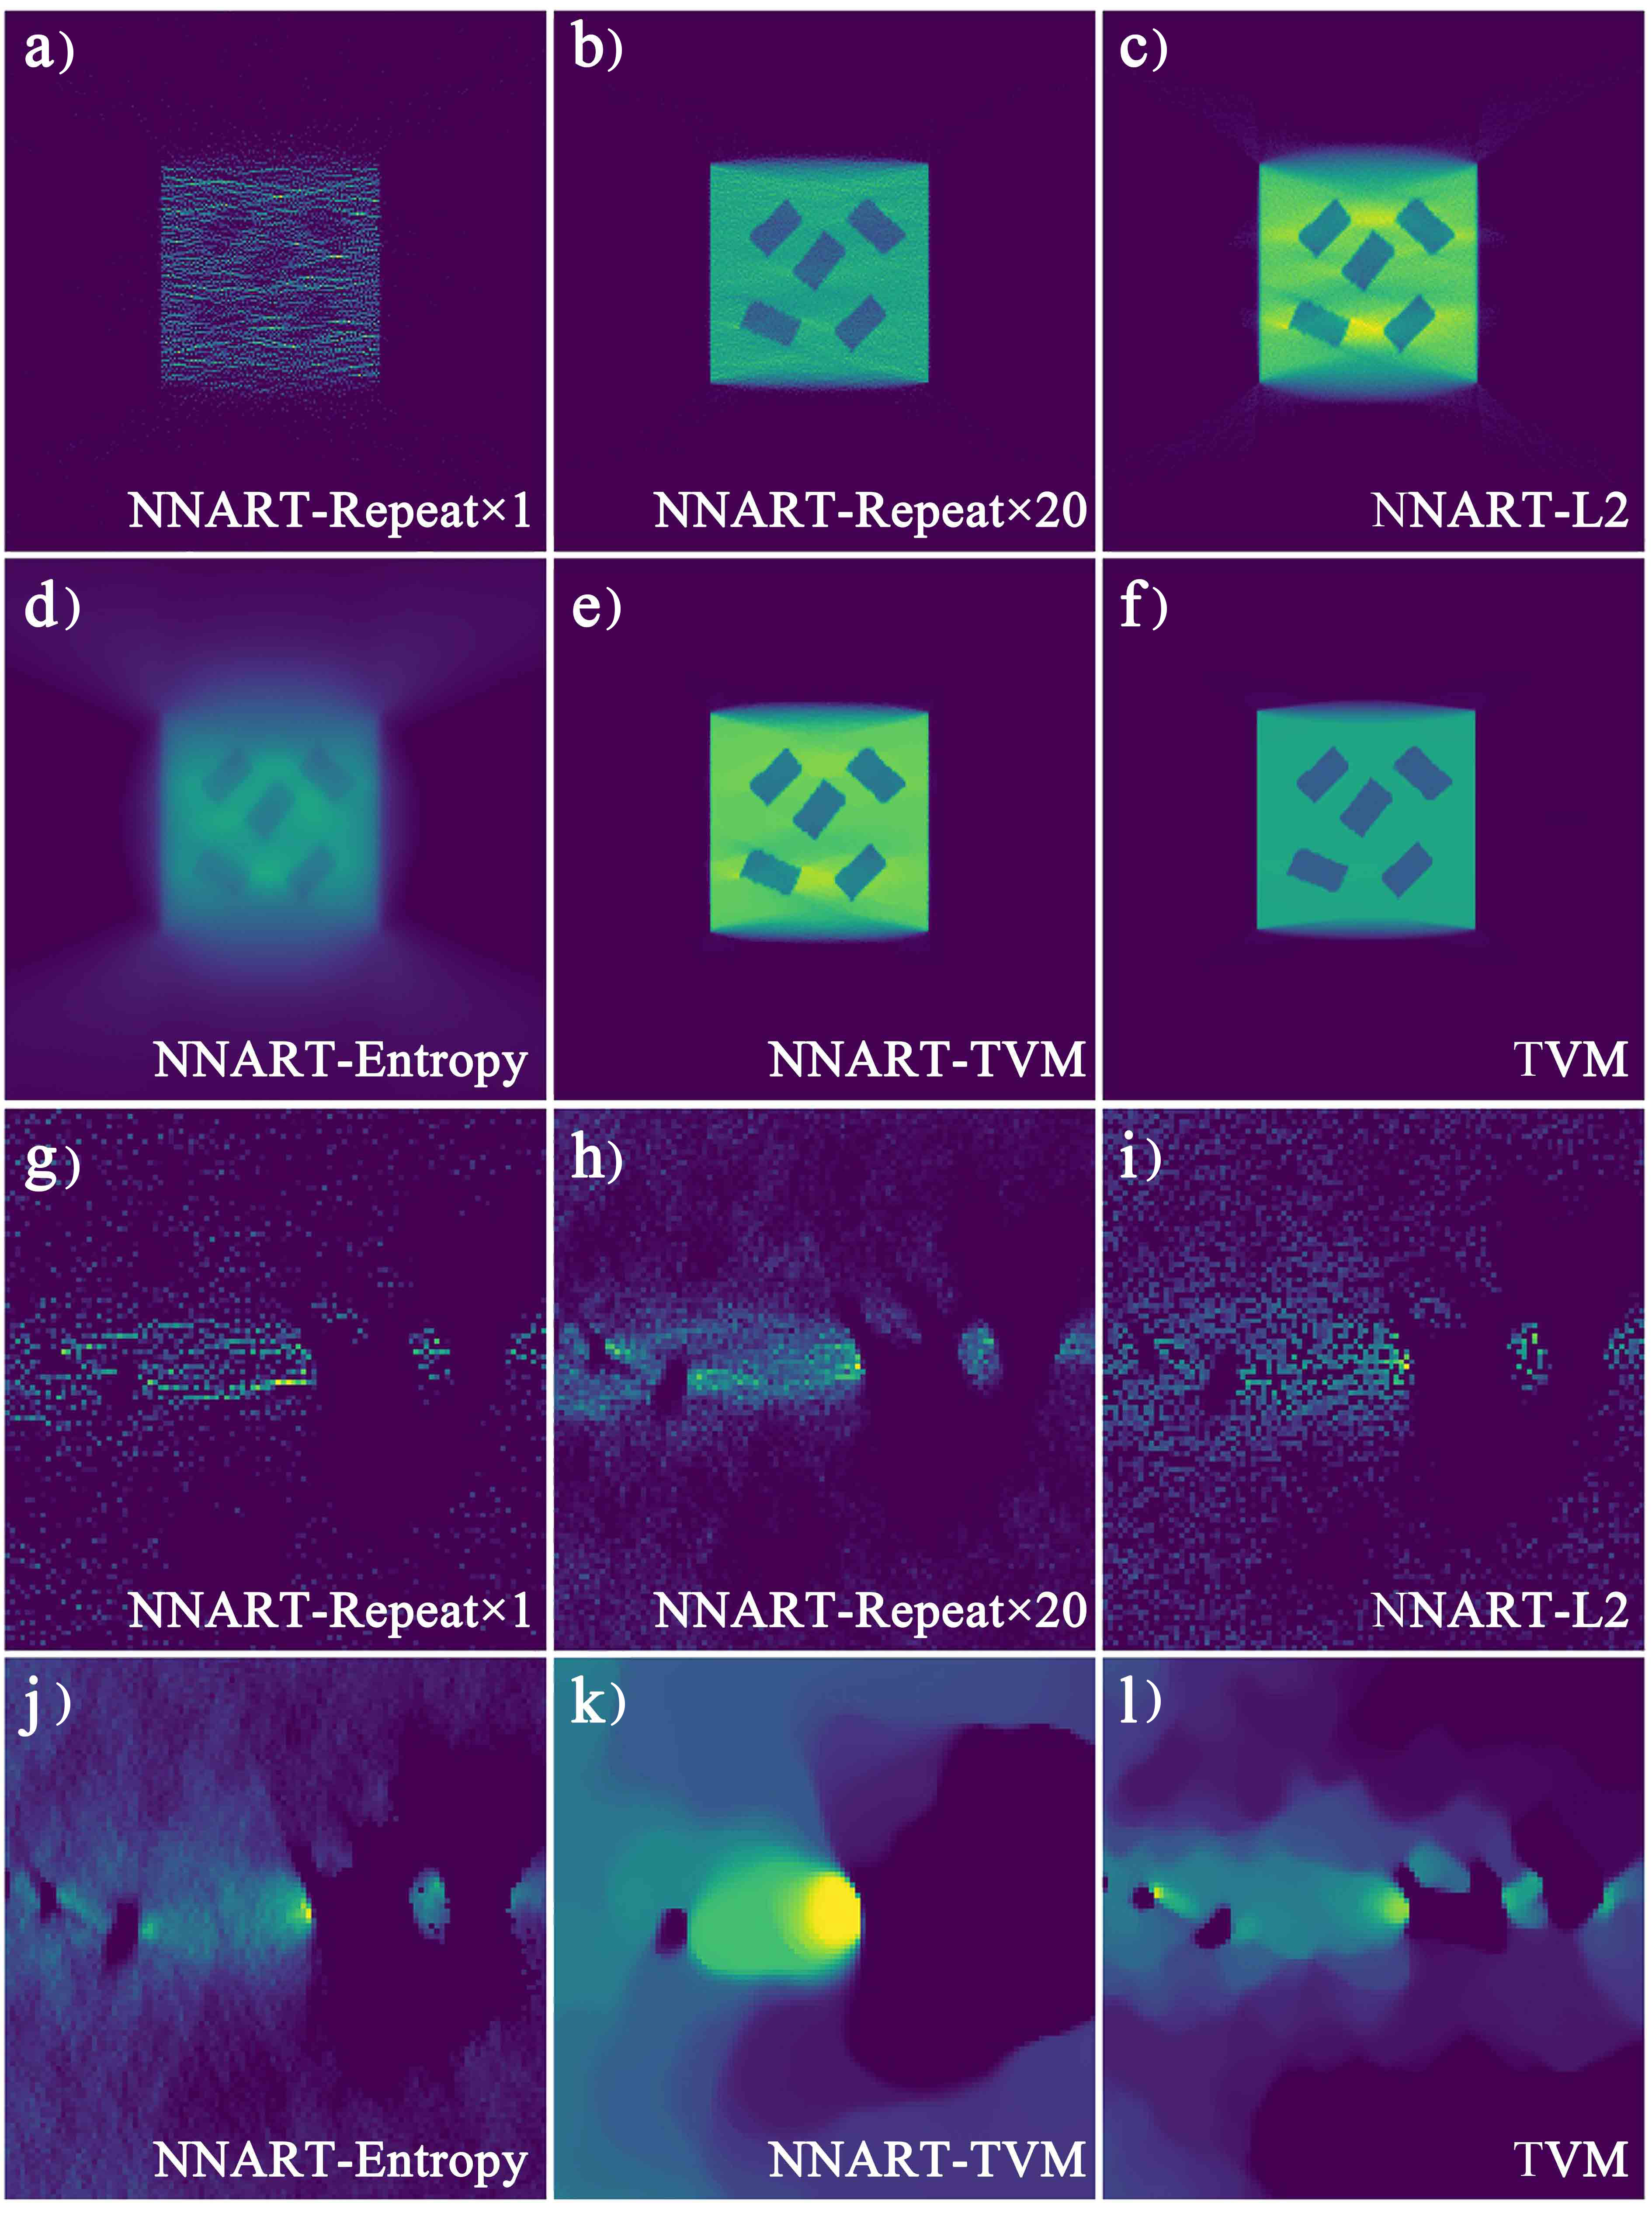
\includegraphics[width=1.0\textwidth]{../3.11/311}
	\caption{NNART 正则化与非正则化下的重构结果对比}\label{fig:311}
	\song\tuzhu{a-f) NNART 一次重构、20 次重构平均、L2 正则化、最大熵正则化、TVM 正则化以及 TVM 算法的模型 1 的重构结果;g-l) NNART 一次重构、20 次重构平均、L2 正则化、最大熵正则化、TVM 正则化以及 TVM 算法的 SiC 片层的重构结果}
\end{figure}

图 2.16 以模型 1 以及图 2.12 中使用的 SiC 样品中的某一层为例,对比了 NNART 在仅重构一次、取 20 次重构平均以及不同正则化项下的重构结果。图 2.16a 和 g 是 NNART 一次重构的结果,如第 2.3.1 条所述,该结果中存在非常严重的噪音。而如图 2.16c-e 所示,在 NNART 经过正则化后,仅需一次重构就能得到平滑解。与图 2.16b 和 f 对比可知,对于模型 1 这种形貌较为简单,投影数据理想的情形而言,NNART 在 L2 和 TVM 正则化下,都具有一定的抑制缺失锥假象的作用,不过 L2 的效果稍差。而 NNART 在最大熵正则化后,虽然能够获得平滑解,但是缺失锥假象的抑制作用完全丧失,其重构结果基本与传统算法 WBP、SIRT 等的结果无异。当使用正则化后的 NNART 重构 SiC 的实验数据时,重构结果则没有如此理想。图 2.16i 展示了 L2 正则化下的 NNART 重构结果,无论如何调节算法的学习率和正则化因子,重构结果中总是会出现严重的椒噪音,所以这种方法基本无法用来处理实验数据。而最大熵正则化下的重构结果(如图 2.16j 所示)则与模型 1 的重构情形一致,缺失锥假象没有得到任何抑制。图 2.16k 则是 NNART 在 TVM 正则化下的重构结果,该结果基本丧失了样品的细节。无论如何调节重构的参数,TVM 正则化后的 NNART 均无法很好地重构该实验数据,甚至在学习率偏大时会出现与图 2.16i 一样的椒噪音。



在 NNART 算法中,存在的较大的问题就是如何获得平滑解。正则化和“多次平均”是两种不同的解决问题的思路。正则化方法的优点是速度快,因为使用正则化后仅需一次重构就能得到平滑解。正则化在许多问题中均具有广泛的应用,同样地,在 NNART 算法中,当问题较简单时,正则化方法可以又快又好地得到平滑的、抑制了假象的重构结果。但是在 SiC 实验数据中,它无法很好地进行重构。所以,多次重构平均是更保险的一种选择。



当样品形貌较为简单时,正则化的 NNART 也能够获得不错的重构结果。图 2.17 展示了铝合金中析出相的 FBP、NNART 最大熵正则化、TVM 正则化的重构结果。图 2.17a-c 是三个重构结果的三维渲染图,从图中可以看出,析出相的形状尽管各不相同,但是都呈颗粒状,这种情况下缺失锥造成的假象相对较弱,重构难度不大。而这三种方法重构的结果基本一致,不过在一些颗粒的局部区域,如三图中的蓝色箭头所指处,FBP 的重构结果中衬度弱或不均匀,而这种现象在其他两个重构结果中得到了改善。图 2.17d-f 展示了图 2.17a-c 中黑色虚线处片层的二维重构图像。在图像的中间有一个体积较大的析出相,并且该析出相的纵横比相对较大,在图 2.17d 中可见析出相的上边界并不清晰,存在较严重的缺失锥假象。而在图 2.17e、h 中,该析出相的边界和周围的噪音分离,其形状较为清晰,所以缺失锥假象在一定程度上被抑制了。



该结果证明,在一般的纳米颗粒的重构中,NNART 的正则化方法也是一种良好的 3DET 替代方案。尽管神经网络的运算需要消耗一定的算力,但是在现代的计算机设备的运算能力下,不使用多次重构平均的 NNART 算法能够符合一般的应用需求。

\begin{figure}[htbp]
	\vspace{\baselineskip}
	\centering
	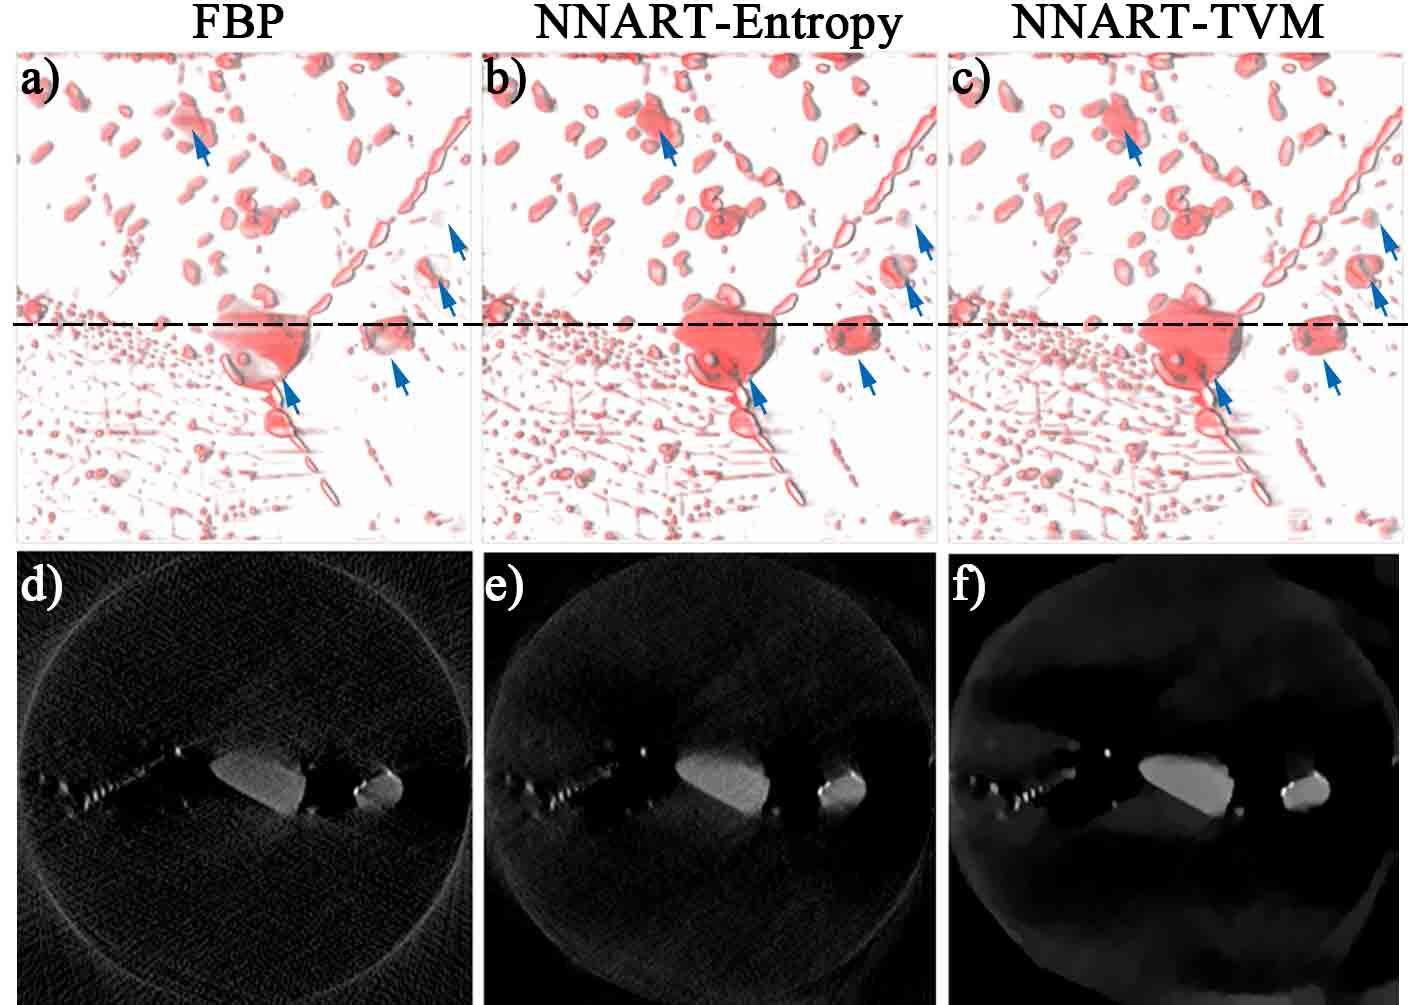
\includegraphics[width=0.85\textwidth]{../3.12/312}
	\caption{FBP、NNART 最大熵和 TVM 正则化重构铝合金析出相的结果对比}\label{fig:312}
	\song\tuzhu{a-c) FBP、NNART 最大熵和 TVM 正则化重构铝合金析出相的三维渲染图;d-f) 图 a、b、c 中黑色虚线处对应的片层的重构结果}
\end{figure}

\section{讨论}

\subsection{重构的精度与速度}
本章的研究内容主要围绕 NNART 抑制缺失锥假象这个主题。本节将简要论述 NNART 与其他主流三维重构算法的速度与精度,主要以 FBP、SIRT、TVM、DART 和 NNART 为例。其中,FBP 属于解析算法,是最简单的算法,SIRT 是 ART 等代数法的代表。而 TVM 和 DART 是典型的基于 SIRT 等迭代算法的约束或正则化方法。

这些方法运算速度的差异较大。对于重构一张 256 像素 $\times$ 256 像素的图像而言,在相同的计算机硬件条件下(比如因特尔 i7 系列的台式机中央处理器),FBP 能够在瞬间完成重构。SIRT、TVM、DART 的重构时间与具体参数选择有
很大关系,但一般在 1$\sim$10 分钟内可以完成重构,不过算法的复杂度是依次升高的。NNART 则需要更久的时间。不过,目前主流的计算机设备都配备有图形处理器。使用图形处理器加速,NNART 一般可以在 2 分钟以内完成一张 256 像素 $\times$ 256 像素图形的重构(一次重构)。真正制约 NNART 运算速度的是“多次平均”,尽管这些“多次”重构之间是相互独立的,可以同时进行,但这并不经济。

理论上,FBP 等解析法的滤波器(filter)只是对点扩散函数解卷积的近似,只有在具备足够多的全角度投影的情况下能够得到精确的重构结果。相同条件下,SIRT 的重构精度更高,当然这是用消耗更多运算资源所换取的。TVM 和 DART 等约束方法针对具有特定性质的材料提出,当重构对象符合这些算法的先验知识时,能够取得很好的重构结果,否则重构结果可能是错误的。而“多次平均”的 NNART 算法摒弃了这些先验知识条件,所以在应用上不受限制,当然其高精度的重构也是通过消耗更多运算资源得到的。不过,在图 2.5 的案例中,也发现 NNART 在某些情况下会出现过拟合现象,影响重构结果的强度分布。总体而言,更高的重构精度需要通过消耗更多的计算资源来实现。并且,讨论重构的精度时必须结合具体应用案例,比如对于原子分辨率的三维重构而言,重构的目标是原子的位置而非形貌,而更广泛的块体材料的三维重构的应用一般仅分析材料的三维形貌。真正重构材料物理性质的三维强度分布的应用案例(比如图 2.9 中的强度梯度)是罕见的。清楚地区分“物理精度”与“数学精度”是做好研究的基础。

\subsection{算法的优势与应用}
非线性神经网络能够对任何函数进行建模。当与反传播技术结合使用时,它可以建立实验投影数据与目标物体之间的关系。在重建过程中,可以从有效的实验数据中推断出缺失锥中丢失的信息。在简单的情况下(例如,图 2.5a),NNART 与正则化迭代方法相比没有明显的优势,因为此时正则化项与实际情况非常吻合。但在如 SiC 实验案例中,样品的实际情况因过于复杂而无法被编码为正则项时,NNART 的优势才会凸显。
NNART 的一种潜在应用是重构烧结陶瓷材料。在这些材料的重构中,TEM 样品的基体陶瓷相会遭受严重的缺失锥假象的影响。在材料科学中,这个问题尚未引起足够的重视,因为大量的 3DET 应用重构的对象是纳米颗粒或析出物,其中出现缺失锥假象可以通过简单的图像分割被去除。第 2.4 节证明了 NNART 的高重构精度,无论嵌入在基体中或基体之间的精细微观结构可以都被精确地重构出来。这有望揭示材料的微观结构和性能之间的定量关系。

\subsection{算法的设计与改进}

本研究将神经网络用作一种优化方法,以代数求解方式解决 3DET 重构问题。为此,整个模型应该由具有 $N^2$ 个节点的输出层的网络,适当的损失函数和优化算法组成。广泛使用的反向传播全连接神经网络是满足要求的众多网络体系结构之一。在大量模拟和实验案例的验证测试之后,我们确定了所提出的 NNART 的每个步骤(包括网络构型,激活函数,损失函数和梯度下降算法)。常用的 sigmoid 激活函数不适用于当前应用,因为它限制输出值小于 “1”,并且可能会遇到梯度消失的问题。Relu 函数适用于 3DET 的问题,因为它在作为激活函数的同时,又是重构结果的非负约束。 Adagrad 算法通过自动调整每个权重和偏置的学习率,可以使重构更快地收敛。而神经网络的构型应具有更多的选择。SiC 样品的成功重构进一步证明了 NNART 在复杂实验数据上的适用性。

通常,在图像特征提取的应用中,卷积神经网络优于前馈神经网络。但是,在当前问题中,输入层是没有意义的。网络的重要性源于其拟合物体的密度函数的能力。从这个角度看,卷积神经网络似乎没有明显的优势。

不同构型的神经网络都有可能实现与 NNART 相同的重构结果。但值得注意的是,许多常用的神经网络中的函数和算法都是专门为深度学习而设计的。因此,为 3DET 问题开发特定的激活函数或优化算法或许是下一步改进 NNART 的方式。

\section{本章小结}
本章提出了一种 ART 型的神经网络 3DET 重构算法以抑制缺失锥假象。该算法利用神经网络的高维度优势进行拟合优化,从有限的信息中外推出了原本丢失的信息,解决较低维度的 3DET 图像重建问题,相对传统的 3DET 重构算法具有以下特点和优势:

(1)NNART 可以大幅度地抑制缺失锥假象,在一定频率范围内恢复出样品缺失的信息。

(2)NNART 算法不同于其他抑制缺失锥假象的算法,它在重构过程中不借助任何先验知识。

(3)在算法中使用了“多次平均”的方式达到求平滑解的目的,相比于使用正则化等方法而言,这种方式使算法对噪音更加稳健。

(4)NNART 算法在一些缺失锥假象严重,或假象与噪音混合的情况下,更能显示其优势。这解决了一些陶瓷材料基体的强度比内部的相或者孔隙强所导致的严重的缺失锥假象的问题。

% !Mode:: "TeX:UTF-8"

\clearemptydoublepage
\chapter[景深对 HAADF-STEM 原子分辨率三维重构的影响]{景深对 HAADF-STEM 原子分辨率\\三维重构的影响}
\section{引言}
3DET 是通过物体沿不同方向的投影来重构物体内部三维结构信息的方法~\cite{Frank2006,Kubel2005},在利用透射电镜研究材料三维微观结构方面有广泛的应用。HAADF-STEM 信号来源于高角度的散射电子,这些电子主要与样品中的原子核发生卢瑟福散射,散射角度主要受到样品中原子序数的影响。因此,其信号强度在一级近似下与样品内原子的原子序数呈线性关系~\cite{Midgley2003}。一般认为 HAADF-STEM 像属于质厚衬度成像,即为样品内部结构的线性投影。因此,HAADF-STEM 像被广泛地应用于 3DET 之中。

随着像差校正 TEM 设备和技术突飞猛进的发展,STEM 能够产生的会聚电子束斑越来越小,从而使 HAADF-STEM 像的二维空间分辨率能够达到 1 埃以下,可以清晰地分辨原子~\cite{Haider1998,Hosokawa2013}。近年来,利用原子分辨率 HAADF-STEM 倾转系列像进行原子分辨率三维重构的工作被陆续报道~\cite{Miao2016,Xu2015,Scott2012,VanAert2011,Lu2015,Azubel2014},对理解材宏观料性能与其微观结构之间的关系具有重要指导意义。然而,原子分辨率的三维重构依然是一项具有挑战性的工作,其难点不仅仅在于实验数据的收集,还在于对 STEM 倾转系列像 3DET 技术缺乏透彻的理论理解。当 STEM 的电子束斑的横向分辨率达到埃量级及以下时,其纵向景深也会减小至纳米量级。此时,HAADF-STEM 像将不再是整个样品内部结构的线性投影,而会转变为样品内部某一深度的光学层析~\cite{Xin2009,Ishikawa2015,Yang2015,Borisevich2006-1,Bosch2020},不再符合倾转系列三维重构对线性投影的要求。因此,在已有的理论模拟和实验结果中,样品的厚度均小于电子束的景深~\cite{Xu2015,VanAert2011,Aveyard2016}。Robert Hovden 等~\cite{Hovden2014}认为当景深小于样品的厚度时,倾转系列三维重构将不可实现。为了突破样品大小的限制,他们提出结合系列欠焦图像来获得足够的样品信息以供三维重构。无独有偶,C. Jacobsen~\cite{Jacobsen2018}提出利用 ptychography 技术,在每个投影方向收集多个厚度层的投影信息来弥补样品信息的不足。然而到目前为止,景深对原子分辨率三维重构的影响尚没有太多研究,人们对原子分辨率 3DET 在理论上的认识还存在不足。

本章通过多层法 STEM 图像模拟和 3DET 重构,研究了纳米尺度景深下原子分辨率 3DET 的可行性,并讨论了景深对原子分辨率 3DET 的影响。结果表明,当景深小于样品厚度时,三维重构技术只能正确重构样品中的局部区域。该区域的大小与入射电子束景深呈正相关,位置与入射束的欠焦量有关。另外,研究还发现实际正确重构的区域相对于电子束名义聚焦位置偏上,即存在提前聚焦现象。

\section{图像模拟与三维重构}
\subsection{HAADF-STEM 倾转系列像的多层法模拟}
HAADF-STEM 图像的多层法模拟计算始于二维的入射会聚电子束束斑波函数方程 $\psi_0$,它的具体表达式如下~\cite{Kirkland2011,Aveyard2016,Tanaka1999}:
\begin{equation}
\psi_0(\boldsymbol{r}) = A_pFT^{-1}\left\{\exp\left[-i\chi(\boldsymbol{k})\right]\cdot A(\boldsymbol{k})\right\}
\end{equation}
\begin{equation}
A(\boldsymbol{k})=\left\{ \begin{array}{cc} 0, &|\boldsymbol{k}|>\theta /\lambda \\ 1, &|\boldsymbol{k}|\leq \theta /\lambda 
\end{array} \right.
\end{equation}
此处,$\boldsymbol{r}$ 为二维实空间坐标,$A_p$ 是归一化因子,$FT^{-1}$ 表示二维反傅里叶变换, $\boldsymbol{k}$ 是二维倒空间坐标,$A$ 表示聚光镜光阑,$\theta$ 是聚光镜光阑半角,$\lambda$ 是电子束的波长,$\chi$ 表示像差方程。与第 1.2.3 条中的公式(1.11)不尽相同,本研究忽略了除欠焦量以外的像差,因此 $\chi(\boldsymbol{k})= \pi\lambda\Delta f\boldsymbol{k}^2$,$\Delta f$ 是欠焦量。通过调节 $\Delta f$ 可以改变电子束在 $z$ 方向上的聚焦位置。

电子束斑入射到样品某一位置时,与样品的交互作用通过多层法模拟。多层法模拟的方法已经在第 1.2.4.1 款中介绍,这里不再赘述。

由于 HAADF 探测器位于背焦面处,即电子衍射空间,因此末层的出射波函数将通过傅里叶变换得到倒易空间波函数 $\Psi_{ext}(\boldsymbol{k})$,并与探测器函数相作用得到最终的图像散射强度。此外,本研究中以冷冻声子模型~\cite{Wang1998,Alania2018}计算热漫散射~\cite{Hillyard1995} 对图像的影响。

\subsection{景深}
景深,也被称作垂直分辨率,它描述了电子束斑在深度($z$)方向上所能影响的范围,如 P.D. Nellist 等~\cite{Nellist2007}的论文中定义景深是电子束斑在光轴上保持 1/2 最大强度的距离。参考多篇论文,景深的具体表达式如下:
\begin{equation}
\Delta z=\alpha \frac{\lambda}{\theta^2}
\end{equation}
此处,根据不同的定义,$\alpha=1 \sim3.5$~\cite{Ishikawa2015,Nellist2007,Born1980,Lee2013}。从上式可知,电子束的加速电压是影响景深的一个重要因素,高电压获得短波长的电子束的景深较小。另一方面,聚光镜光阑的尺寸决定会聚半角 $\theta$ 的大小,所以它也是影响景深的另一个重要因素。在实际的电镜使用中,聚光镜光阑的作用是阻挡电子束中像差较大的部分,只留下中间像差较小的部分,以获得均匀对称的电子束。所以实际使用的聚光镜光阑的尺寸与电子束中的残余像差有关。在本研究的模拟测试中,为了简化对比,忽略了实际情形中像差与聚光镜光阑的关系,将欠焦量以外的所有像差假设为 “0”,直接根据公式(3.2),模拟不同会聚半角的电子束。不过,根据 Varat Intaraprasonk 等~\cite{Intaraprasonk2008}介绍的优化最佳光阑尺寸的方法,也可以在模拟中考虑像差与聚光镜光阑的关系,得到符合实际的具有像差的入射电子束。

图 3.1 展示了不同加速电压和会聚半角的模拟电子束束斑。图 3.1a 中的会聚半角仅 10 mrad,代表一般的非球差校正电镜的束斑,可见束斑的尺寸非常大,根据公式(3.3)计算得其在加速电压为 200 kV 时的景深为 $25.1 \sim 87.9$ nm。图 3.1b 代表了一般的球差校正电镜的束斑,会聚半角为 30 mrad。它的尺寸相对于会聚半角为 10 mrad 时明显变小,其对应的景深为 $2.8 \sim 9.8$ nm。图 3.1c 代表了先进的球差校正电镜中的束斑,会聚半角进一步增大为 50 mrad,此时景深为 $1.0 \sim 3.5$ nm。作为对比,将其中的加速电压降低至 100 kV 后,如图 3.1d 所示,束斑尺寸相应变大。

\begin{figure}[H]
	\vspace{\baselineskip}
	\centering
	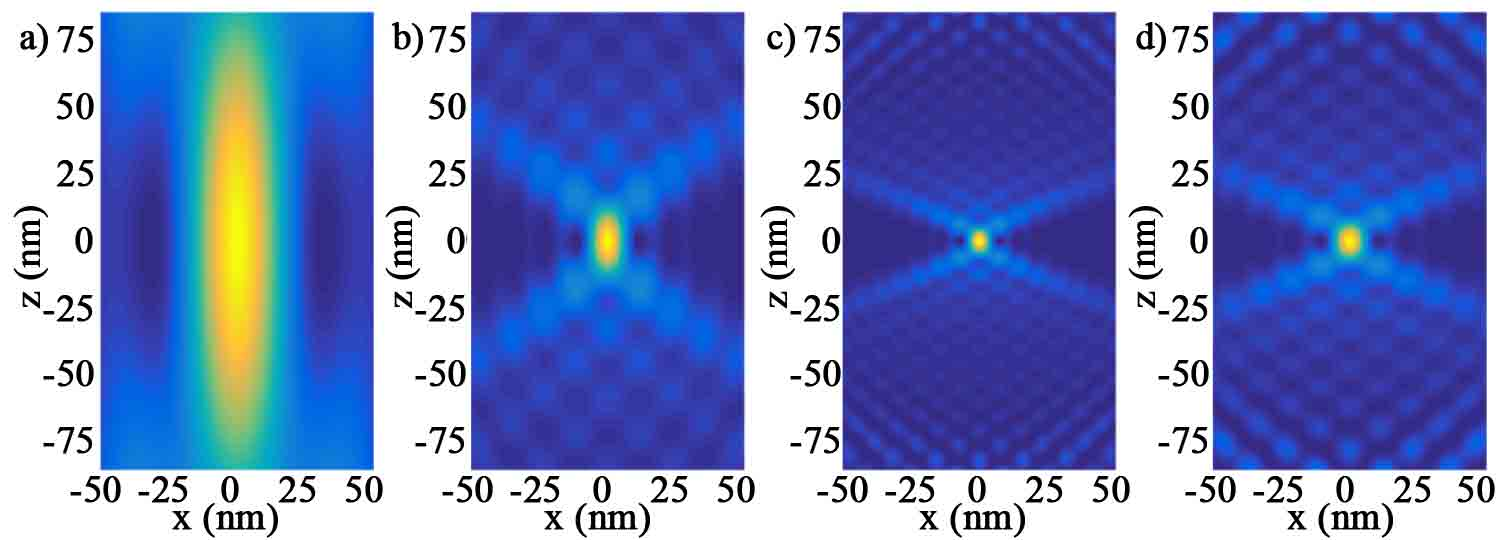
\includegraphics[width=0.9\textwidth]{../4.11/411}
	\caption{不同参数的电子束斑}\label{fig:413}
	\song\tuzhu{a) 加速电压 200 kV,会聚半角 10 mrad;b)  加速电压 200 kV,会聚半角 30 mrad;c)  加速电压 $\textnormal{200 kV}$,会聚半角 50 mrad;d) 加速电压 100 kV,会聚半角 50 mrad}
\end{figure}

\subsection{倾转系列三维重构}
在本研究中,倾转系列三维重构是根据 D. Wolf 等~\cite{Wolf2014} 的论文中介绍的同时迭代重构技术实现的。这个技术的核心算法如下所示:
\begin{equation}
f_t=f_{t-1}+\omega\mathcal{R}^{-1}\left(\hat{f}^{exp}-\mathcal{R}f_{t-1}\right)
\end{equation}
其中,$f_t$ 和 $f_{t-1}$ 是第 $t$ 和 $t-1$ 次重构的结果,$\mathcal{R}$ 和 $\mathcal{R}^{-1}$ 分别表示拉登变换和反拉登变换,$\hat{f}^{exp}$是实验倾转系列像,$\omega$ 是收敛因子。该算法通过本实验室编写的代码实现,对模拟的 HAADF-STEM 倾转系列像进行重构。

\subsection{计算模型与参数}
本章利用图像模拟生成样品沿不同方向的 STEM 图像,并利用这些图像进行三维重构,讨论景深对原子分辨率三维重构的影响。图  3.2 展示了用于计算的样品模型。为了避免通道效应~\cite{WangA2010,Sinkler1999}对三维重构带来的假象,该模型的原子在 $x-z$ 面内处于无序状态,如图 3.2a 所示。另外,由于样品 $x-z$ 方向被真空层包裹,由图像模拟的周期性重复假设所引起的环绕效应~\cite{Kirkland2010}可以被忽略。该无序原子模型的总尺寸是 $15 \textnormal{ nm} \times 15 \textnormal{ nm} \times 2.4 \textnormal{ nm}$,中间样品的尺寸是 10 nm $\times$ 10 nm $\times$ 2.4 nm(下文中的尺寸均指中间样品的尺寸)。在图像模拟测试中,电子束沿 $z$ 轴入射。由于块体三维重构可视为多个二维重构图像的有序堆叠,因此本章只重构二维图像中的其中一层,如图 3.2b,c 所示。从图 3.2b 可以看出,样品中各原子均严格处于一个 $x-z$ 平面内,这便于对重构的结果进行分析。图 3.2c 展示了该原子层的原子结构图。从图中可以看出,样品在 $x-z$ 面内的周期性被破坏,因此模拟过程中不存在通道效应。

\begin{figure}[H]
	\vspace{\baselineskip}
	\centering
	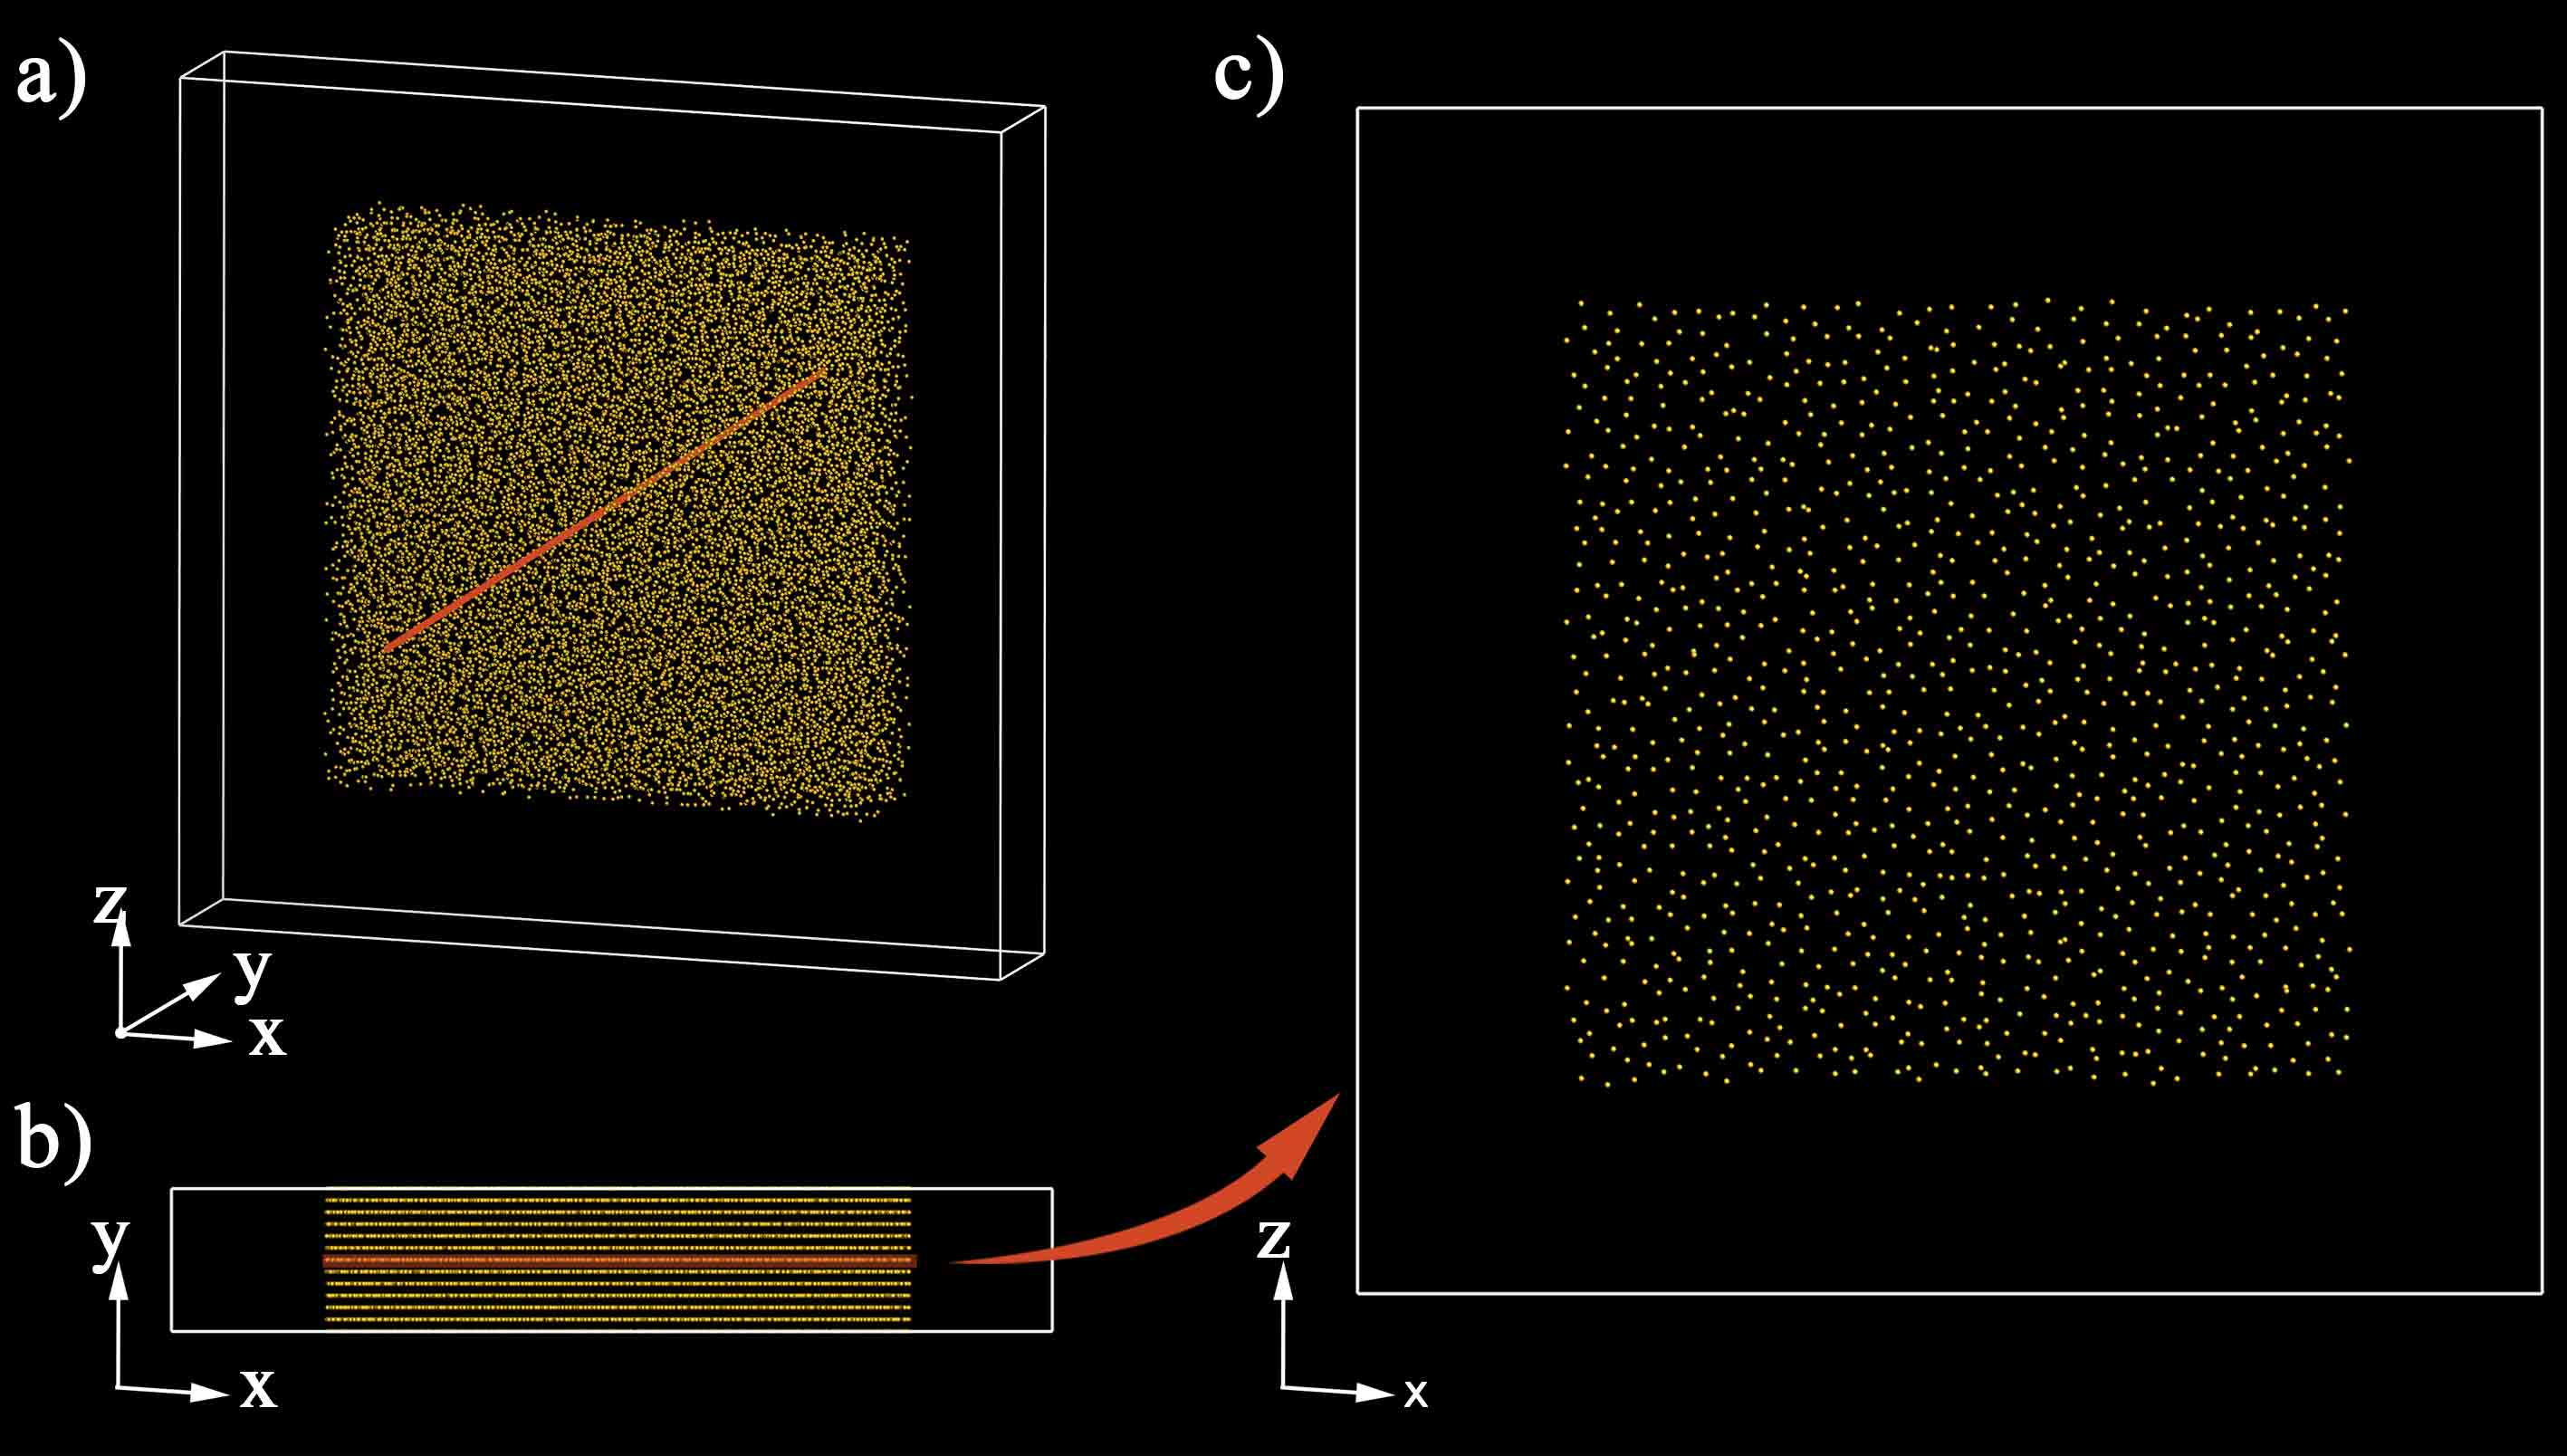
\includegraphics[width=0.85\textwidth]{../4.1/41}
	\caption{用于图像模拟的三维模型}\label{fig:41}
	\song\tuzhu{a) 原子模型侧视图,图中橙线表示倾转轴;b) 原子模型顶视图,橙线代表中间原子层;c) 图 b 中橙线所标志的中间原子层的正视图}
\end{figure}

在多层法模拟中,电子束斑的采样为 $512\times 512$ 像素,对应实际尺寸 2.4 nm $\times$ 2.4 nm,在倒空间中足以完整计算 267.7 mrad 之内的信息。欠焦量以外的像差如前所述均设置为“0”。HAADF 探测器收集角为 $90\sim230$ mrad,冷冻声子模型声子态为 16。会聚半角、加速电压、欠焦量、模型的厚度和原子序数是本研究的对比参数。多层法像模拟通过本实验室编写的代码实现,其中使用了图形处理单元计算加速技术~\cite{MWQ2018}。倾转系列像的倾转角为 -90º 至 +89º,倾转间隔 1º。

此外,为了对比,本章还用同样的方法建立了尺寸为 5 nm $\times$ 5 nm $\times$ 2.4 nm 和 2.4 nm $\times$ 2.4 nm $\times$ 2.4 nm(不包含真空层的尺寸)的无序原子模型。

\section{结果与分析}
\subsection{局部区域重构现象}
图 3.3 是将会聚半角为 50 mrad,加速电压为 200 kV (此时的景深为 $1.0 \sim 3.5$  nm)的入射束,聚焦到尺寸为 10 nm $\times$ 10 nm $\times$ 2.4 nm 的铝原子模型内 1/4、1/2 和 3/4 深度时的重构结果。从图 3.3a-c 可知,当电子束斑的景深小于样品的厚度时,样品局部区域的原子位置仍可被清晰地重构,且该正确重构的区域随电子束斑聚焦的位置而移动。

\begin{figure}[H]
	\vspace{\baselineskip}
	\centering
	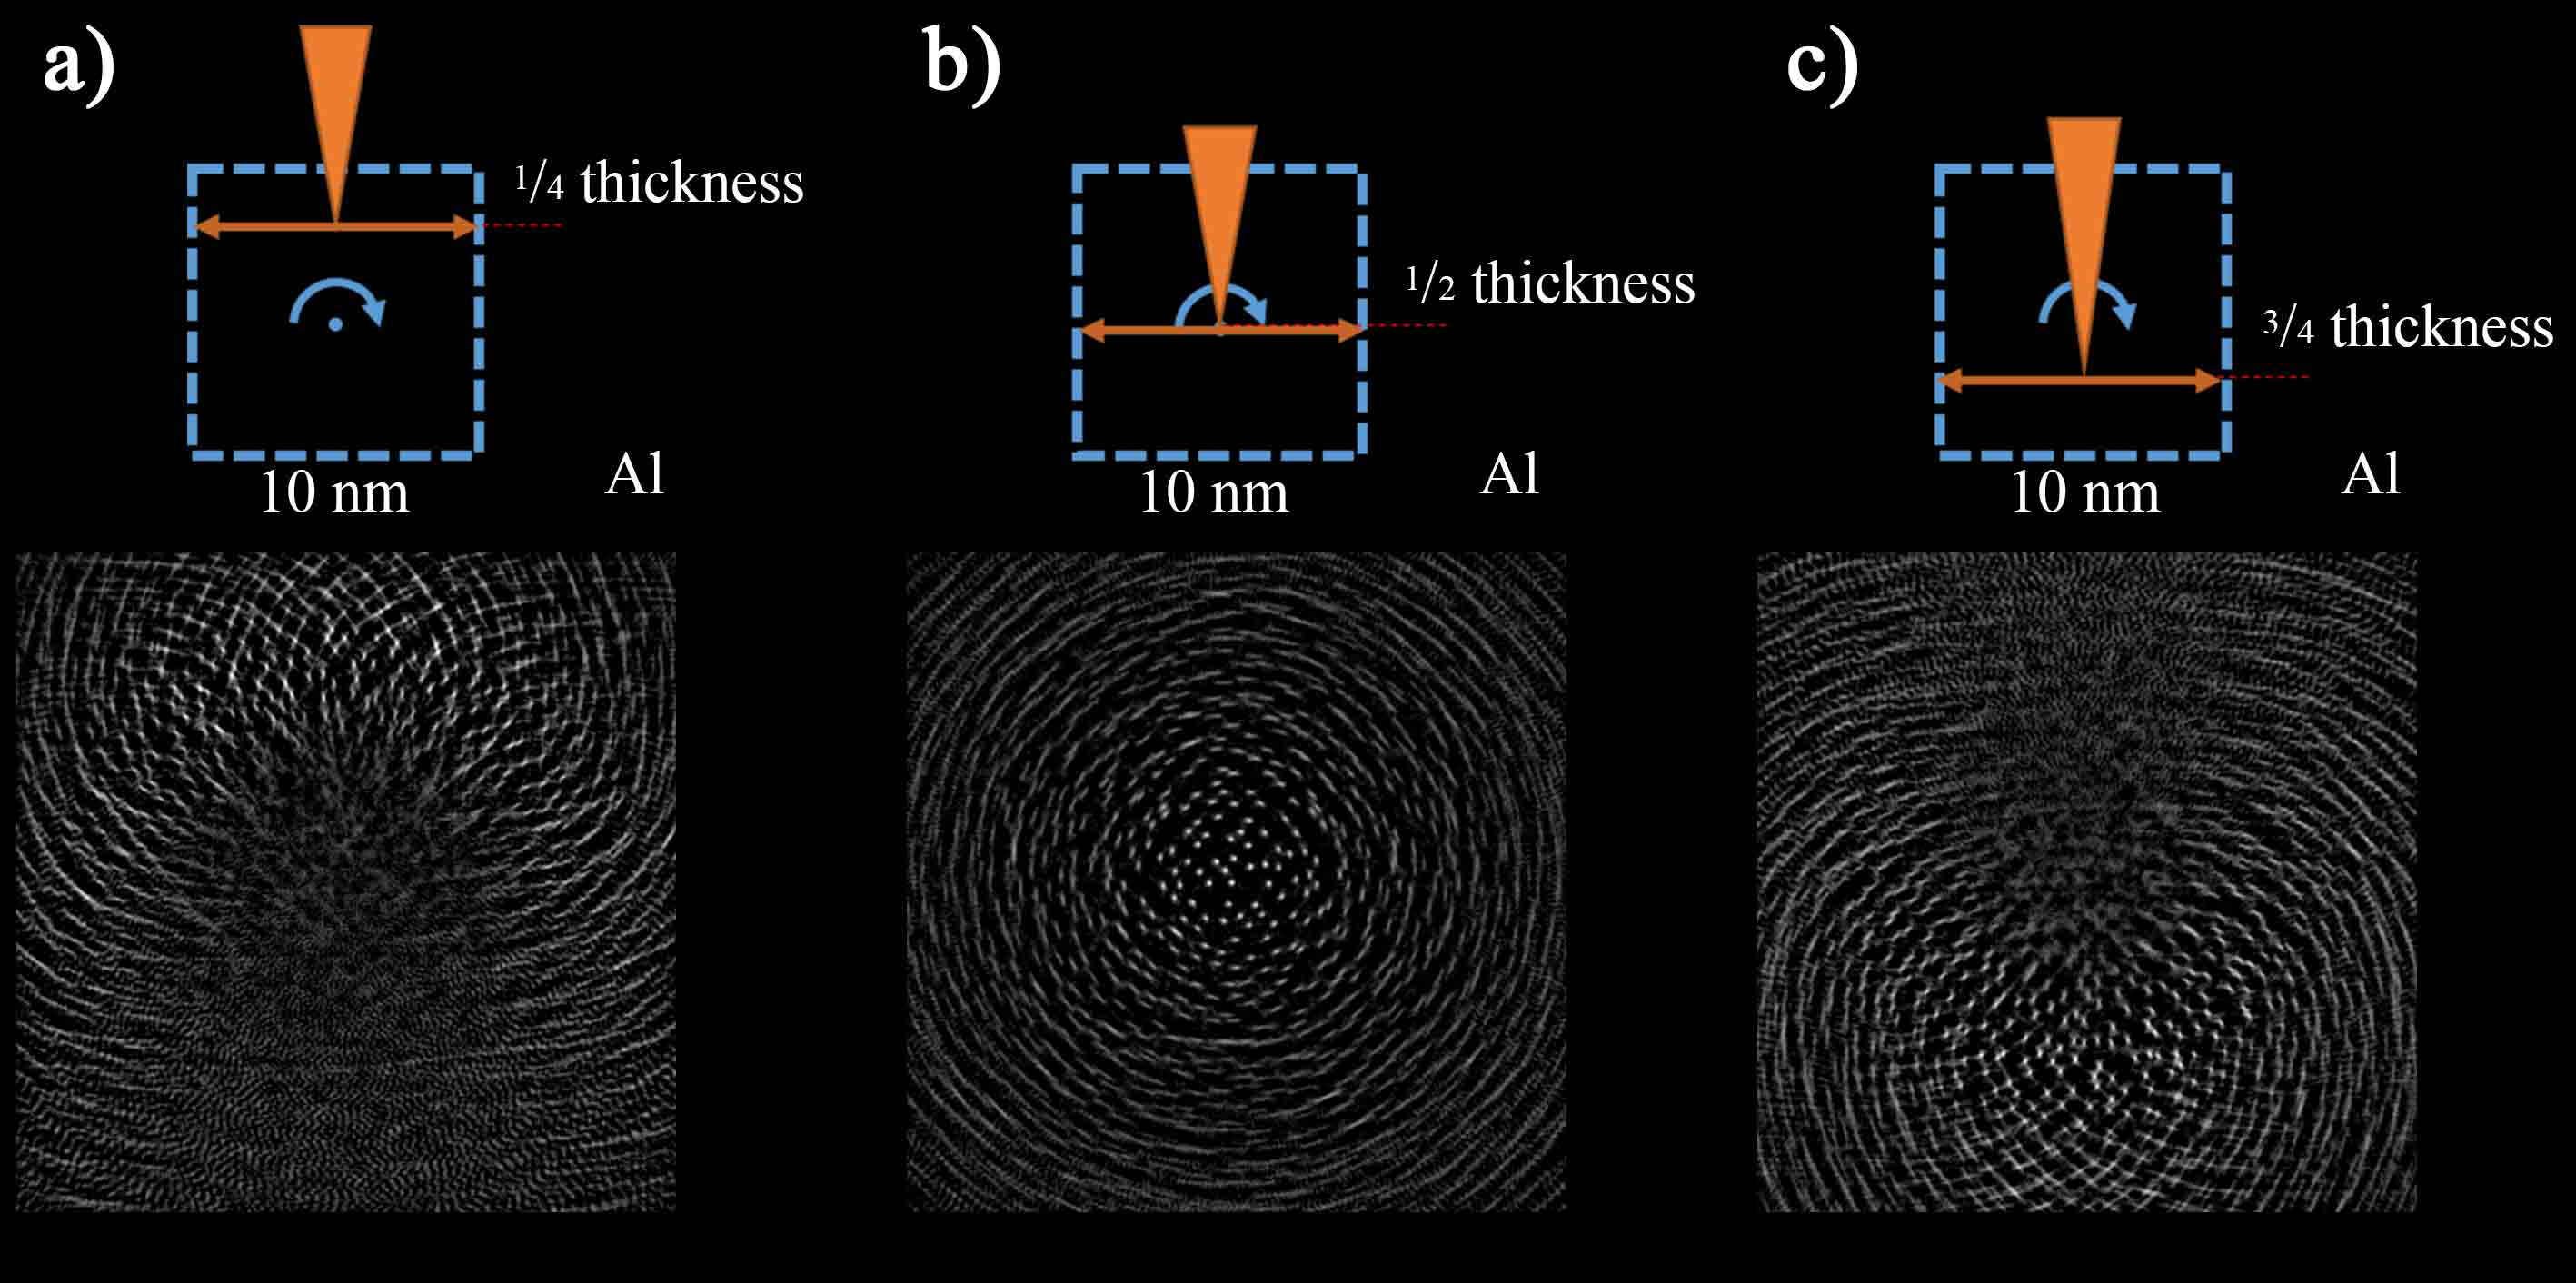
\includegraphics[width=0.85\textwidth]{../4.2/42}
	\caption{尺寸为 10 nm $\times$ 10 nm $\times$ 2.4 nm 的铝原子模型的重构结果}\label{fig:42}
	\song\tuzhu{电子束斑分别被聚焦到深度为:a) 1/4 样品厚度;b) 1/2 样品厚度;c) 3/4 样品厚度的位置;电子束的会聚半角均为 50 mrad,加速电压是 200 kV}
\end{figure}

图 3.4 是将会聚半角为 50 mrad,加速电压为 200 kV(此时的景深为 $1\sim3.5$ nm)的电子束会聚至尺寸分别为 10 nm $\times$ 10 nm $\times$ 2.4 nm,5 nm $\times$ 5 nm $\times$ 2.4 nm 和 2.4 nm $\times$ 2.4 nm $\times$ 2.4 nm 的铝原子模型内 1/2 深度时的重构结果。在图 3.4a-c中,红色正方形虚线框对应的边长为 2.4 nm,黄色正方形虚线框对应的边长为 5 nm。通过对比可以明显地看出,尽管模型大小不同,在相同的成像条件下,被正确重构出原子位置的区域的尺寸,在三种情况下均接近 2.4 nm。

\begin{figure}[H]
	\vspace{\baselineskip}
	\centering
	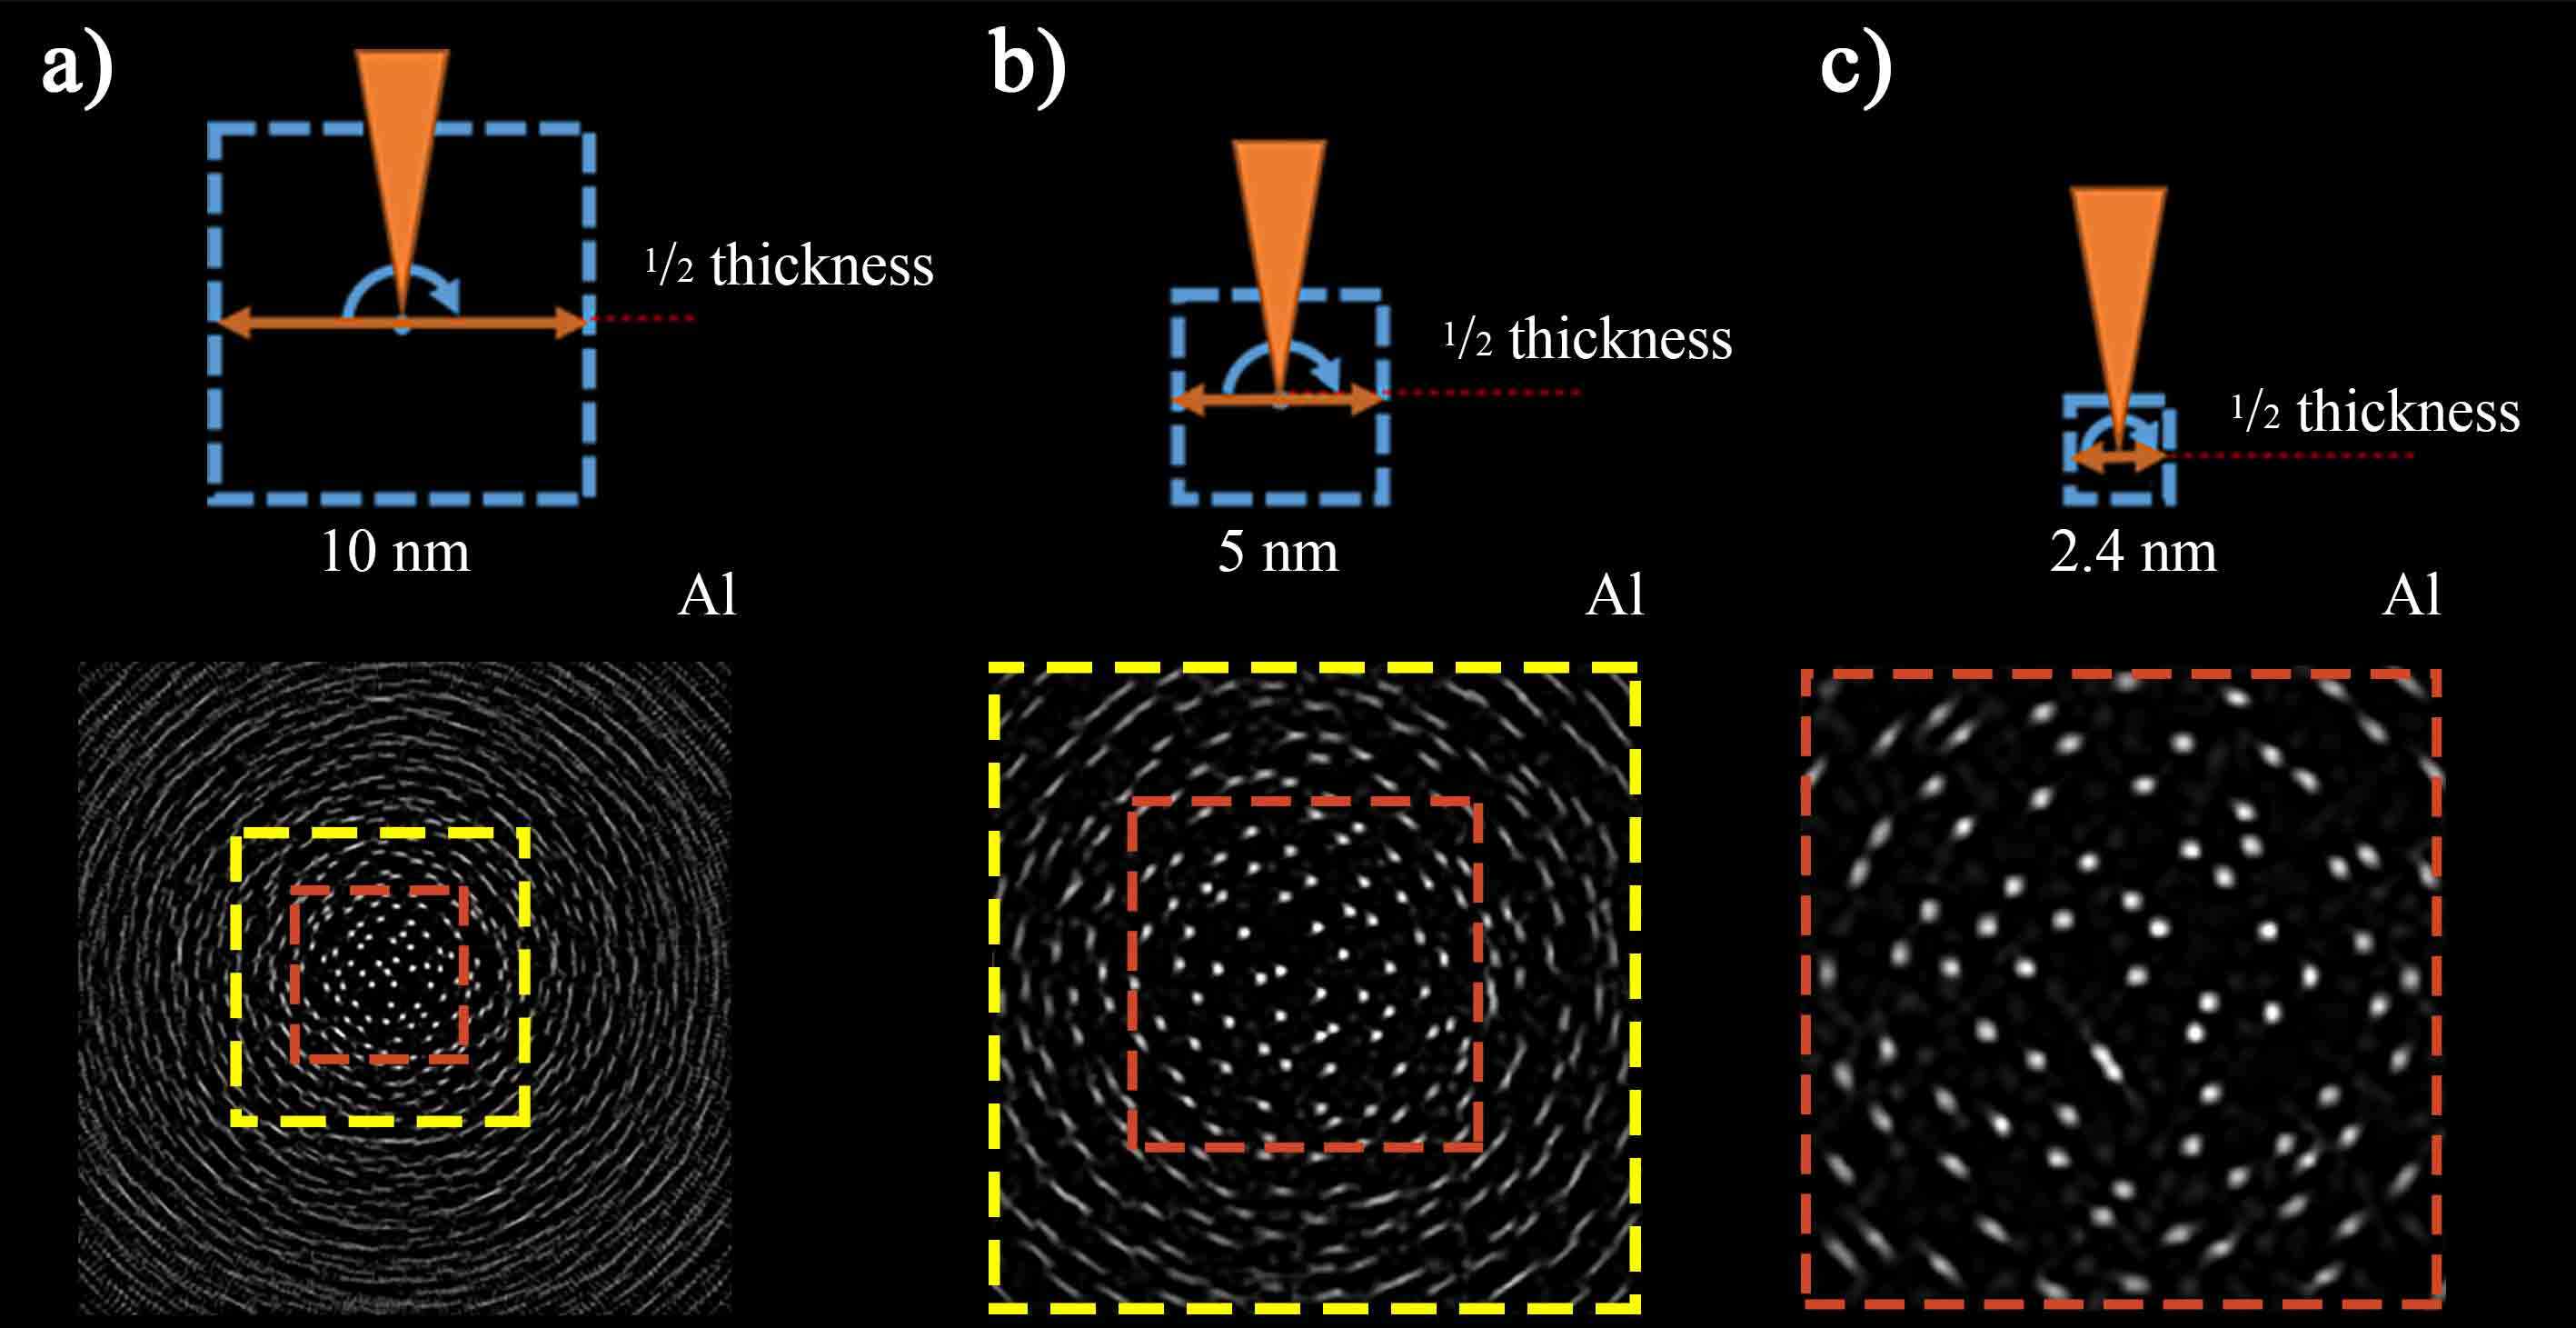
\includegraphics[width=0.85\textwidth]{../4.4/44}
	\caption{不同尺寸模型的重构结果}\label{fig:43}
	\song\tuzhu{a) 10 nm $\times$ 10 nm $\times$ 2.4 nm;b) 5 nm $\times$ 5 nm $\times$ 2.4 nm;c) 2.4 nm $\times$ 2.4 nm $\times$ 2.4 nm;电子束会聚半角均为 50 mrad,加速电压是 200 kV。电子束斑被聚焦到样品厚度 1/2 的深度位置。图中红色虚线框边长的实际长度是 2.4 nm,黄色虚线框边长的实际长度是 5 nm}
\end{figure}





\begin{figure}[H]
	\vspace{\baselineskip}
	\centering
	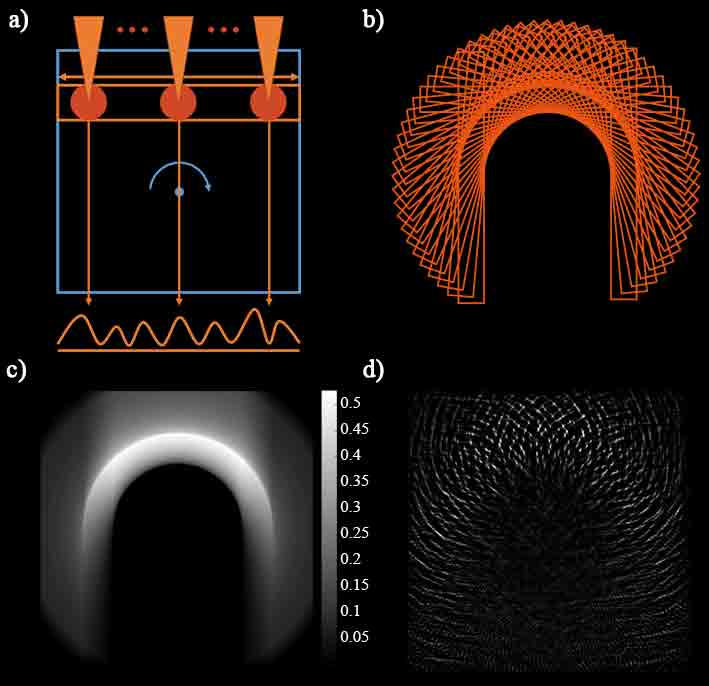
\includegraphics[width=0.9\textwidth]{../4.3/43}
	\caption{电子束景深小于样品厚度时,HAADF-STEM 倾转系列三维重构原理示意图}\label{fig:44}
	\song\tuzhu{a) HAADF-STEM 成像过程,图中橙色圆圈表示景深;b) 倾转系列像中的样品信息在重构时的分布示意图;c) 图 b 对应的信息恢复率;d) 对应情况的模拟重构结果}
\end{figure}

对上述重构结果的解释如图 3.5 所示。图 3.5a 描述了 STEM 图像的形成过程,当电子束斑(即横向分辨率和纵向景深)小于样品厚度时,它在样品中的实际影响范围有限,只能携带样品的局部结构信息,最终形成的扫描图像,仅具有样品中某一深度范围内(橙色矩形框所示)的结构信息,即形成光学层析。该成像模式下产生的倾转系列像,在三维重构的过程,其中包含的样品信息将以如图 3.5b 所示的模式被用于重构。正确的三维重构,需要将每一个倾转角下的图像所携带的样品的结构信息,通过反拉登变换,正确地恢复到对应位置,然后把这些信息叠加。但按照图 3.5b 中的信息恢复方式,样品的信息并不能被完全正确地恢复至正确位置,信息恢复率如图 3.5c 所示。图 3.5d 是该模式下的某一模拟重构图像,对比图 3.5c 和图 3.5d 可知,信息恢复率高的位置,原子可以被正确地重构出来。在图 3.5c 中,信息恢复率最高是 55\%,这说明该位置的重构结果,在 180° 全角度倾转的重构条件下,其实际有效信息仅有 -50° 至 50°,存在严重的缺失锥现象,只是当重构的对象原子的形状为小圆点时,缺失锥效应不严重。进一步容易知道,信息恢复率和入射电子束聚焦的位置与倾转轴之间的相对位置具有直接关系。当电子束聚焦的位置与倾转轴重合时,如图 3.3b 和图 3.4a-c 中的情形,其重构时的信息覆盖率最高,中心可达 100\%。当电子束聚焦点远离倾转轴时,重构的质量会变差。另外,显然的是,正确重构的区域根据电子束聚焦的深度变化,且该区域的尺寸直接决定于电子束的景深。



\subsection{提前聚焦现象}
电子束在不同材料中的传播情况是不同的。图 3.6 对比了将会聚半角均为 $\textnormal{50 mrad}$,加速电压为 200 kV 的电子束,分别聚焦到尺寸均为 10 nm $\times$ 10 nm $\times$ $2.4\textnormal{ nm}$ 的铝和金原子(原子序数分别为 13 和 79)模型的 1/2 深度时的重构结果。图 3.6b 是图 3.6a 和 c 中心区域的放大图,其中红色圆点标出了两图中相同原子所在的位置。仔细观察和对比,可以发现,在相同成像条件下,不同元素的原子模型中可以正确重构的区域的尺寸是相近的。不过,这两个区域位置并不重合。在图 3.6b 铝原子模型的重构图中,红色圆点标记的下方仍然存在清晰重构的原子。但图 3.6b 金原子模型的重构图中,红色圆点标记的下方的原子并没有被清晰地重构,但是上方却有更多被清晰重构的原子。直接对比图 3.6a 和 c 也能发现,图 3.6a 中正确重构的区域在图像的中心,而图 3.6c 中正确重构的区域相对偏上。这相当于在图 3.6b 中,电子束斑并不是会聚于样品的中心,而是在上方提前聚焦了。  

\begin{figure}[H]
	\vspace{\baselineskip}
	\centering
	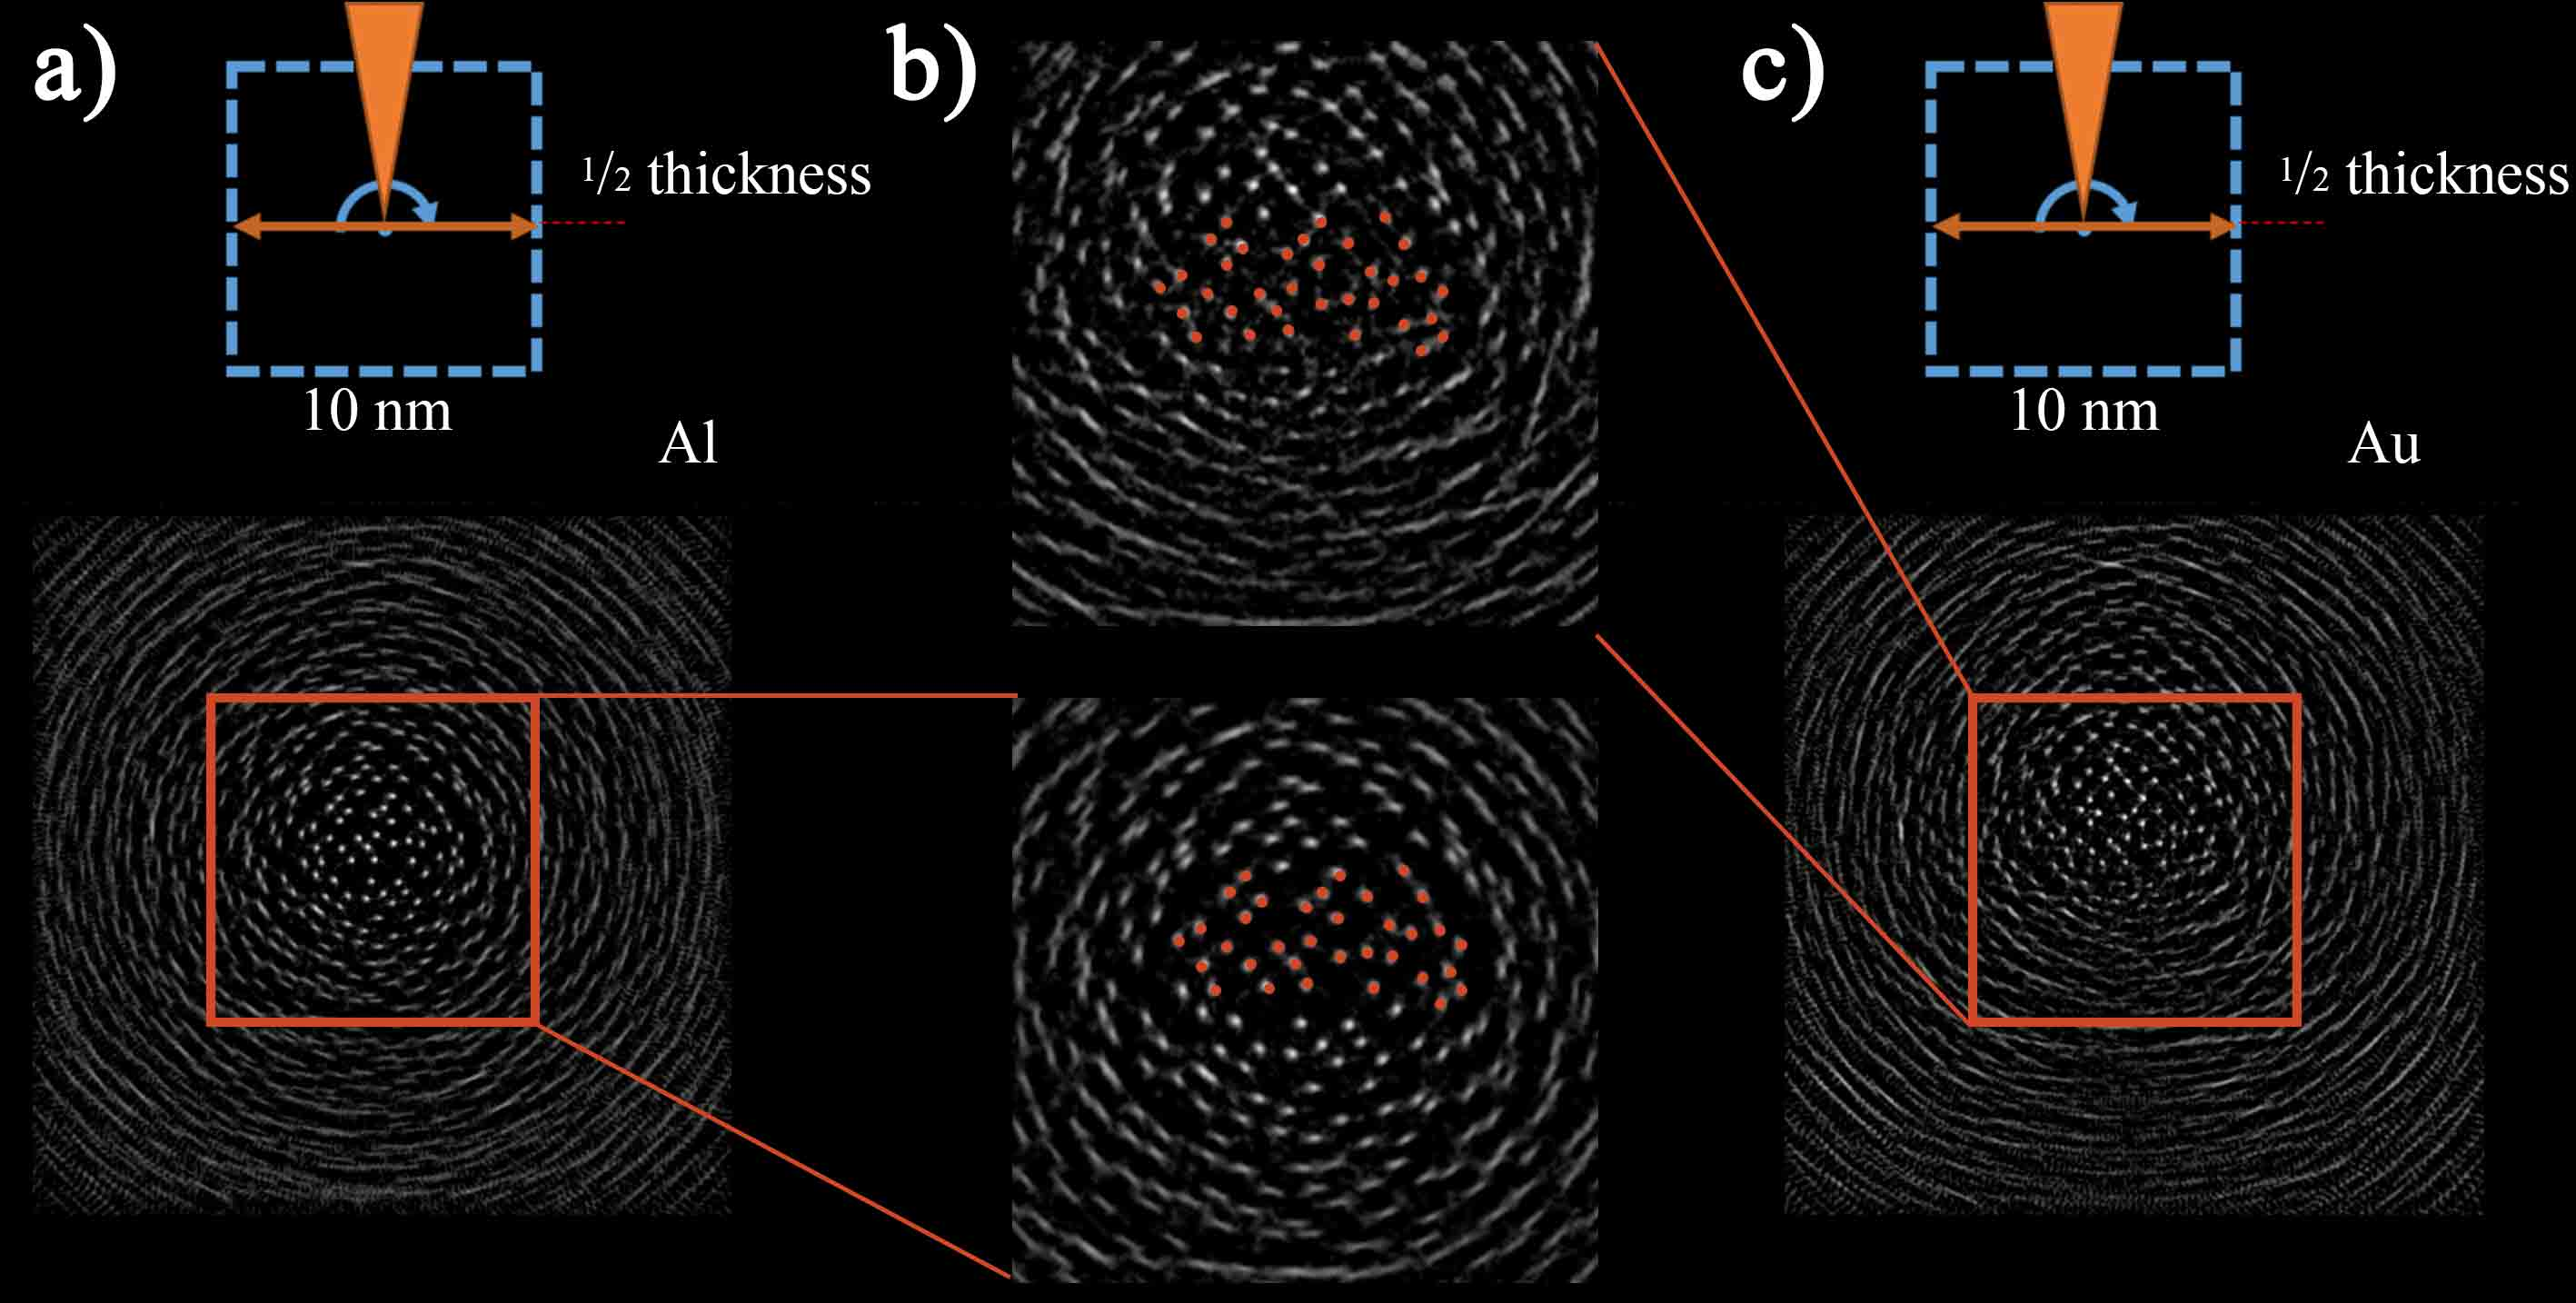
\includegraphics[width=0.9\textwidth]{../4.6/46}
	\caption{提前聚焦现象示意图}\label{fig:45}
	\song\tuzhu{a) 尺寸为 10 nm $\times$ 10 nm $\times$ 2.4 nm 的铝原子模型的重构结果;b) 图 a 和 c 的中心区域放大图,其中红色的圆点表示两个区域中相同的正确重构的原子位置;c) 尺寸为 10 nm $\times$ 10 nm $\times$ 2.4 nm 的金原子模型的重构结果;在模拟中,会聚半角均为 50 mrad,加速电压是 200 kV。电子束斑均被聚焦到样品厚度 1/2 的深度位置}
\end{figure}


图 3.7 更进一步探究了会聚半角和加速电压对提前聚焦现象的影响。图 3.7a-c 对应的参数分别为会聚半角 50 mrad,加速电压 200 kV;会聚半角 30 mrad,加速电压 200 kV;会聚半角 50 mrad,加速电压 100 kV。它们对应的景深分别为 $1。0\sim3.5$ nm,$2.8\sim9.8$ nm,$1.5\sim5.1$ nm。通过对比发现图 3.7b 中正确重构的区域最大,图 3.7a 中正确重构的区域最小,该结果与它们对应的电子束的景深大小相吻合。图 3.7a-c 中正确重构的区域均不在模型的中心处,都发生了提前聚焦的现象,且图 3.7b 中提前聚焦的程度最高。这是因为图 3.7b 对应的电子束的景深最大,能量的集中程度反而最低,因此最容易受到静电势的影响而提前聚焦。

\begin{figure}[htbp]
	\vspace{\baselineskip}
	\centering
	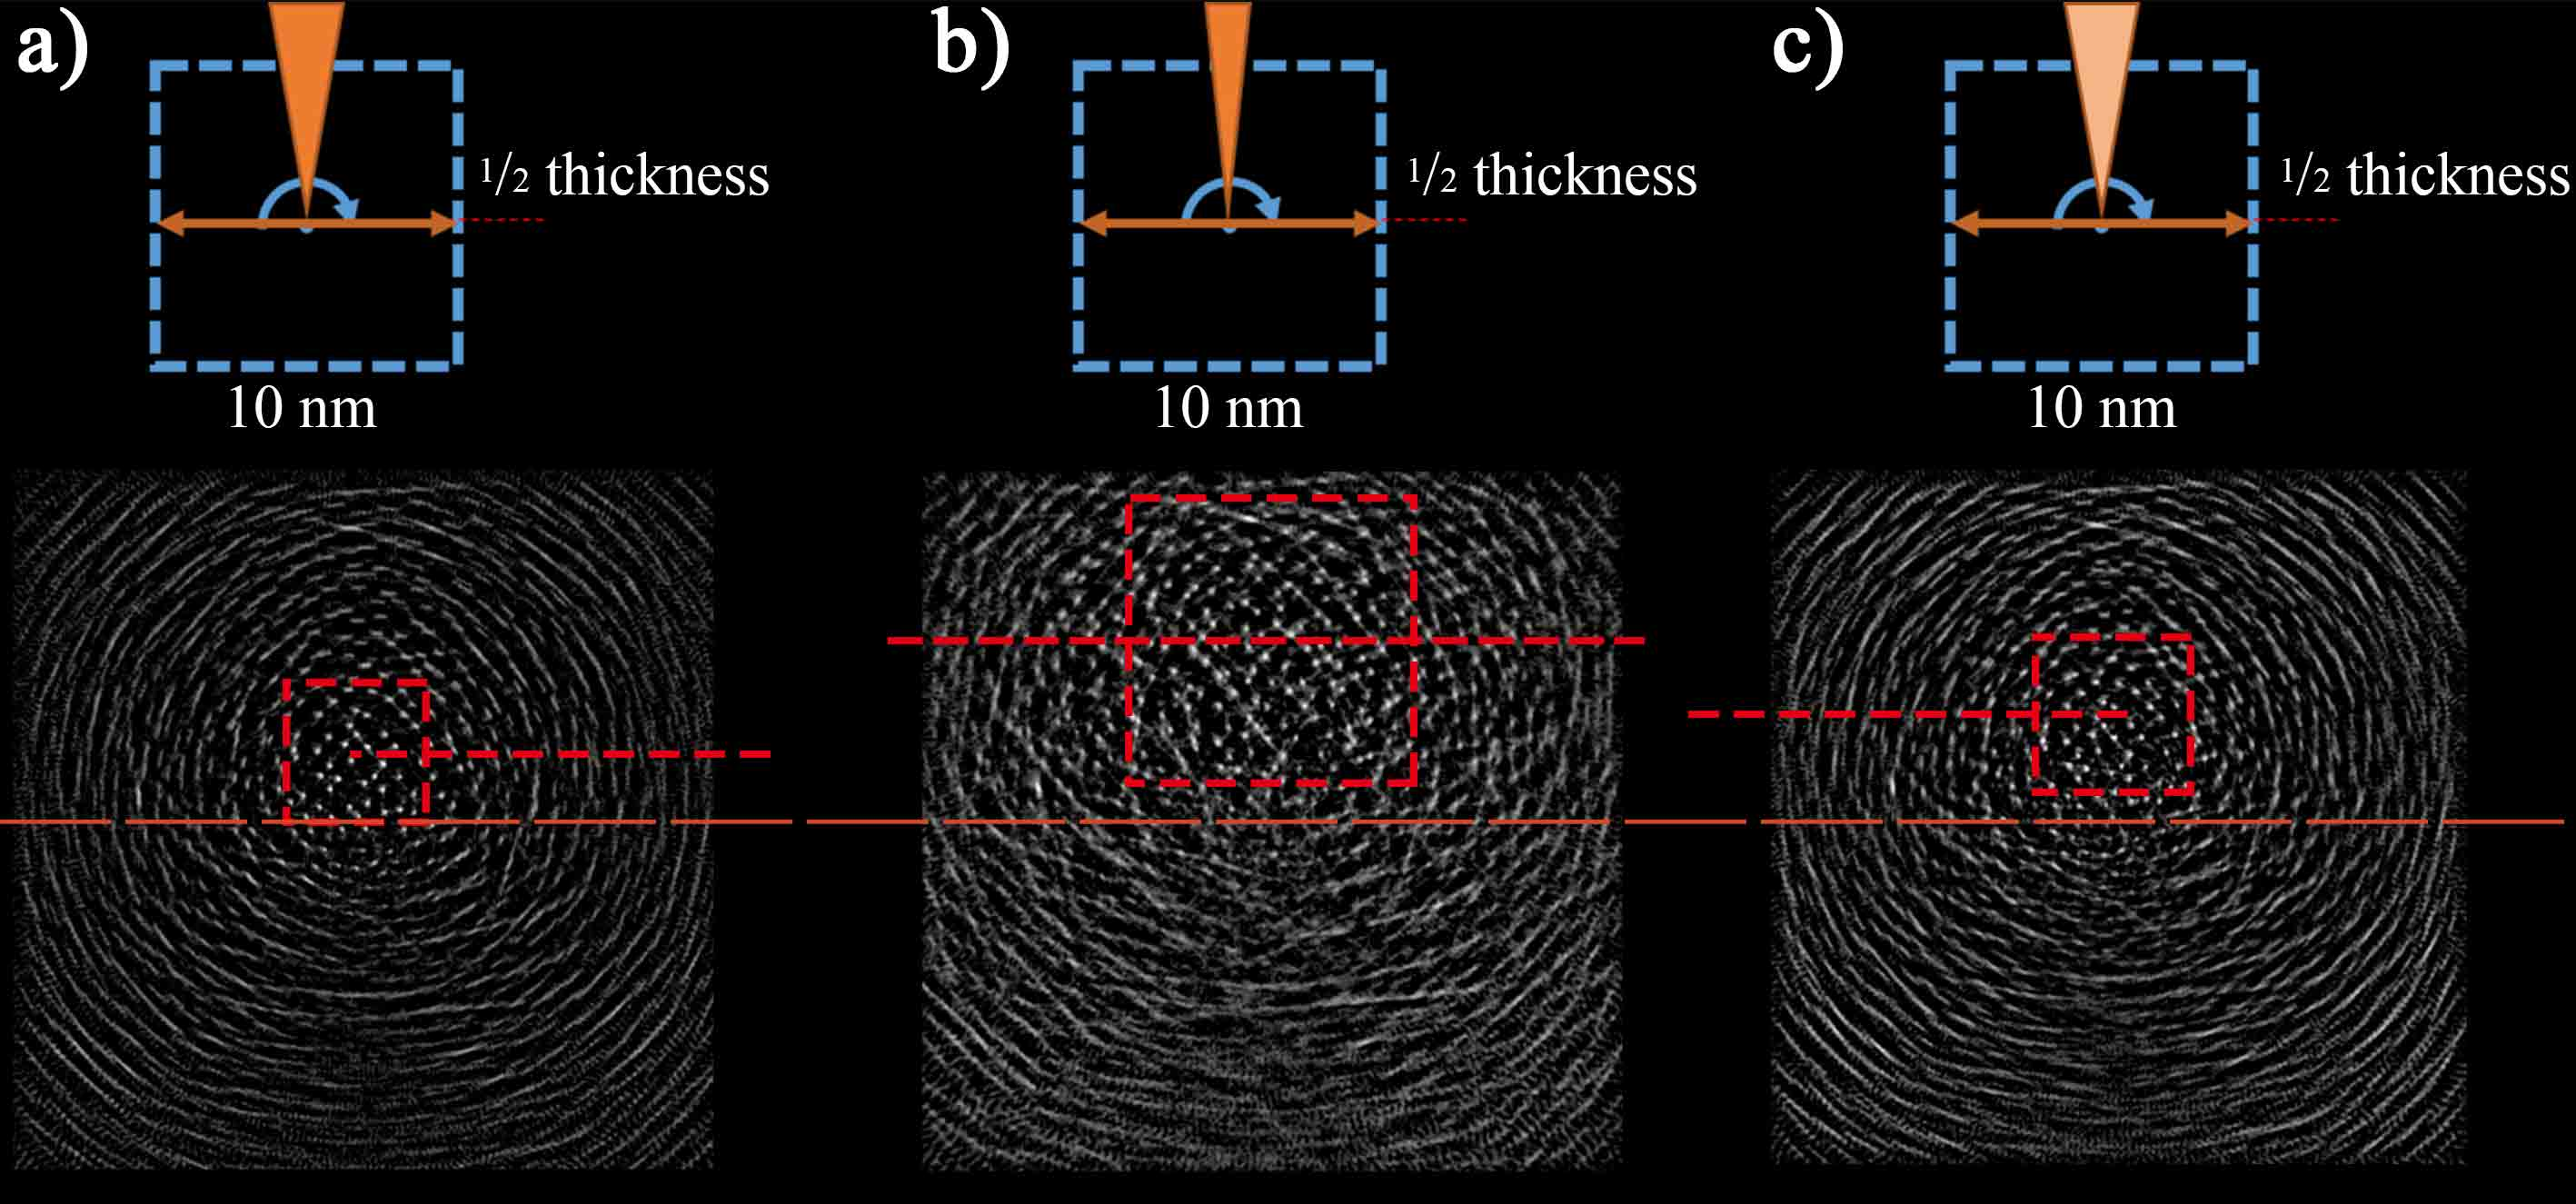
\includegraphics[width=0.9\textwidth]{../4.7/47}
	\caption{不同参数的会聚束引起的提前聚焦现象}\label{fig:46}
	\song\tuzhu{尺寸为 10 nm $\times$ 10 nm $\times$ 2.4 nm 的金原子模型的重构结果:a) 会聚半角均为 50 mrad,加速电压是 200 kV;b) 会聚半角均为 30 mrad,加速电压是 200 kV;c) 会聚半角均为 50 mrad,加速电压是 100 kV;电子束斑均被聚焦到样品厚度 1/2 的深度位置}
\end{figure}

为了加深对这种现象的理解,本研究对电子束斑在不同情况下的强度分布进行了模拟。图 3.8 展示了不同成像参数、不同原子元素下,将电子束名义上聚焦至倾转 30° 的 10 nm $\times$ 10 nm $\times$ 2.4 nm 原子模型的中心(原点 (0, 0))时,电子束斑的实际强度分布情况。在铝原子模型,即图 3.8a 和 c 中,电子束的束斑关于原点呈中心对称分布,其形状与真空中的理想束斑相近。这是因为铝原子的静电势较弱,对电子束斑的强度分布影响较小。因此,在图 3.6a 中没有发现提前聚焦的现象。反观$\textnormal{图 3.8b 和 d}$,两图中的电子束斑的强度分布都发生了扭曲,向上方偏离,这说明金原子的静电势对电子束斑的强度分布产生了较大的影响,最终导致提前聚焦的现象,这与图 3.6c 的结果吻合。对比图 3.8b 和 d 可以发现,当会聚半角为 30 mrad,即电子束会聚程度较低时,束斑的强度中心向上偏离的程度更大,这与图 3.7a 和 b 的结果一致。


\begin{figure}[H]
	\vspace{\baselineskip}
	\centering
	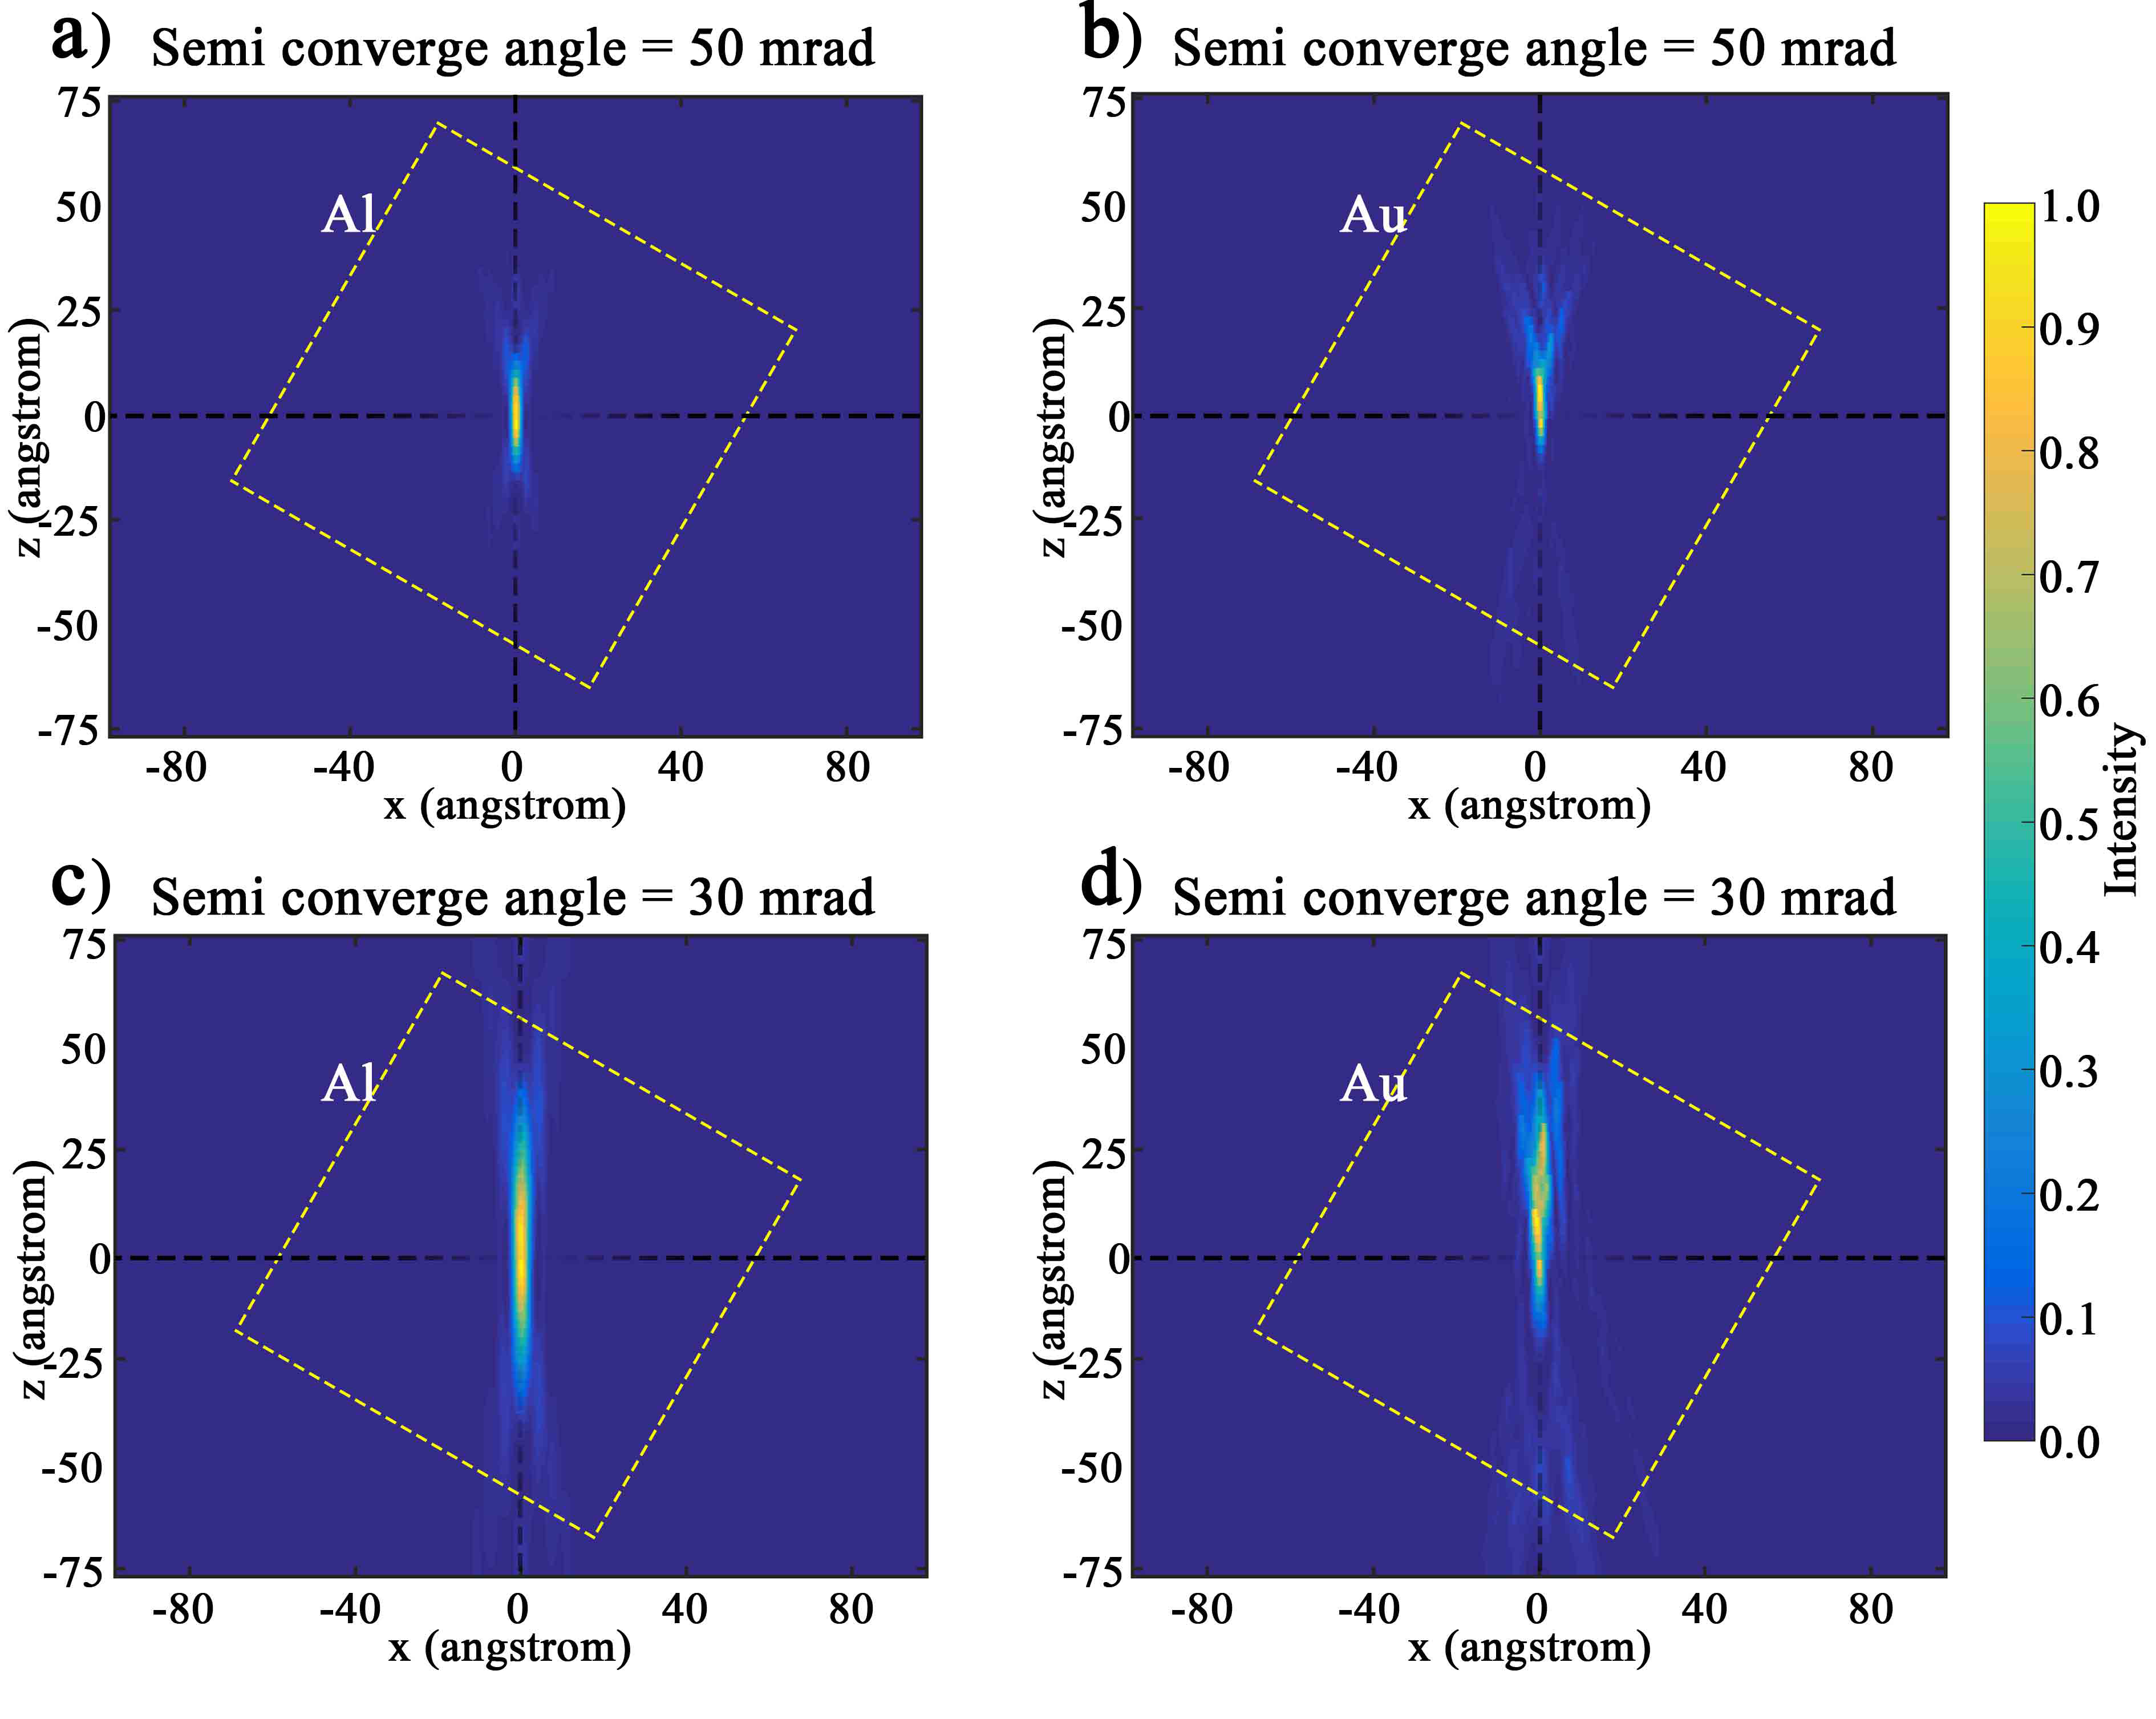
\includegraphics[width=0.9\textwidth]{../4.10/410}
	\caption{电子束聚焦至 10 nm $\times$ 10 nm $\times$ 2.4 nm 的原子模型中心时,电子束斑的强度分布图}\label{fig:47}
	\song\tuzhu{a) 会聚半角为 50 mrad,模型中的原子是铝原子;b) 会聚半角为 50°,模型中的原子是金原子;c) 会聚半角为 30°,模型中的原子是铝原子;d) 会聚半角为 30 mrad,模型中的原子是金原子;加速电压均为 200 kV,模型倾转 30°,原点 (0,0) 是电子束的名义聚焦位置,黄色虚线框表示模型的边缘}
\end{figure}
\subsection{影响分辨率的因素}
STEM 中电子束的强度分布是决定最终三维重构分辨率的重要因素。$\textnormal{图 3.9a 和 c}$ 比较了在将两个不同条件的电子束会聚至 10 nm $\times$ 10 nm $\times$ 2.4 nm 的金原子模型的 1/2 深度时的重构结果,其中电子束的加速电压均为 200 kV。图 3.9a 对应的电子束的会聚半角为 10 mrad,与普通非球差校正电镜(Cs = 1.2 mm)的最优参数相当,其横向分辨率较低,景深较大。将图 3.9a 与原模型比较可以确定整个块体的重构都是正确的,只是原子图像较模糊。而图 3.9c 对应的电子束的会聚半角为 50 mrad,与球差校正电镜的最优成像参数相当,其横向分辨率高,景深小,所以图 3.9c 中只有局部区域被正确地重构,该区域的原子清晰可辨。该对比直观地反映了分辨率与景深之间存在的矛盾。

图 3.9b 展示了将会聚半角 10 mrad,加速电压 200 kV 的电子束聚焦至 5 nm $\times$ 5 nm $\times$ 2.4 nm 的金原子模型中 1/2 深度时的重构结果。可以发现,尽管电子束的分辨率较低,重构图像中的原子是清晰可分辨的,其与图 3.9a 中的结果大不相同。通过对比图 3.9a 和 b,可以发现,同样的成像参数用于不同厚度的样品的三维重构时,重构结果的分辨率是不同的,样品厚度越小,重构分辨率越高。这个结果符合克劳瑟准则~\cite{Crowther1970},详情可见第 1.3.10 条。

图 3.9d 展示了将会聚半角 10 mrad,加速电压 200 kV 的电子束聚焦至 10 nm $\times$ 10 nm $\times$ 2.4 nm 的铝原子模型中 1/2 深度时的重构结果。在轻元素的模型中,尽管电子束的分辨率较低,整个模型中的原子依然都能被清晰地重构出来。该重构结果与图 3.9a 对比可知,实际样品的元素也会影响三维重构的分辨率,轻元素的样品更容易重构。

\begin{figure}[H]
	\vspace{\baselineskip}
	\centering
	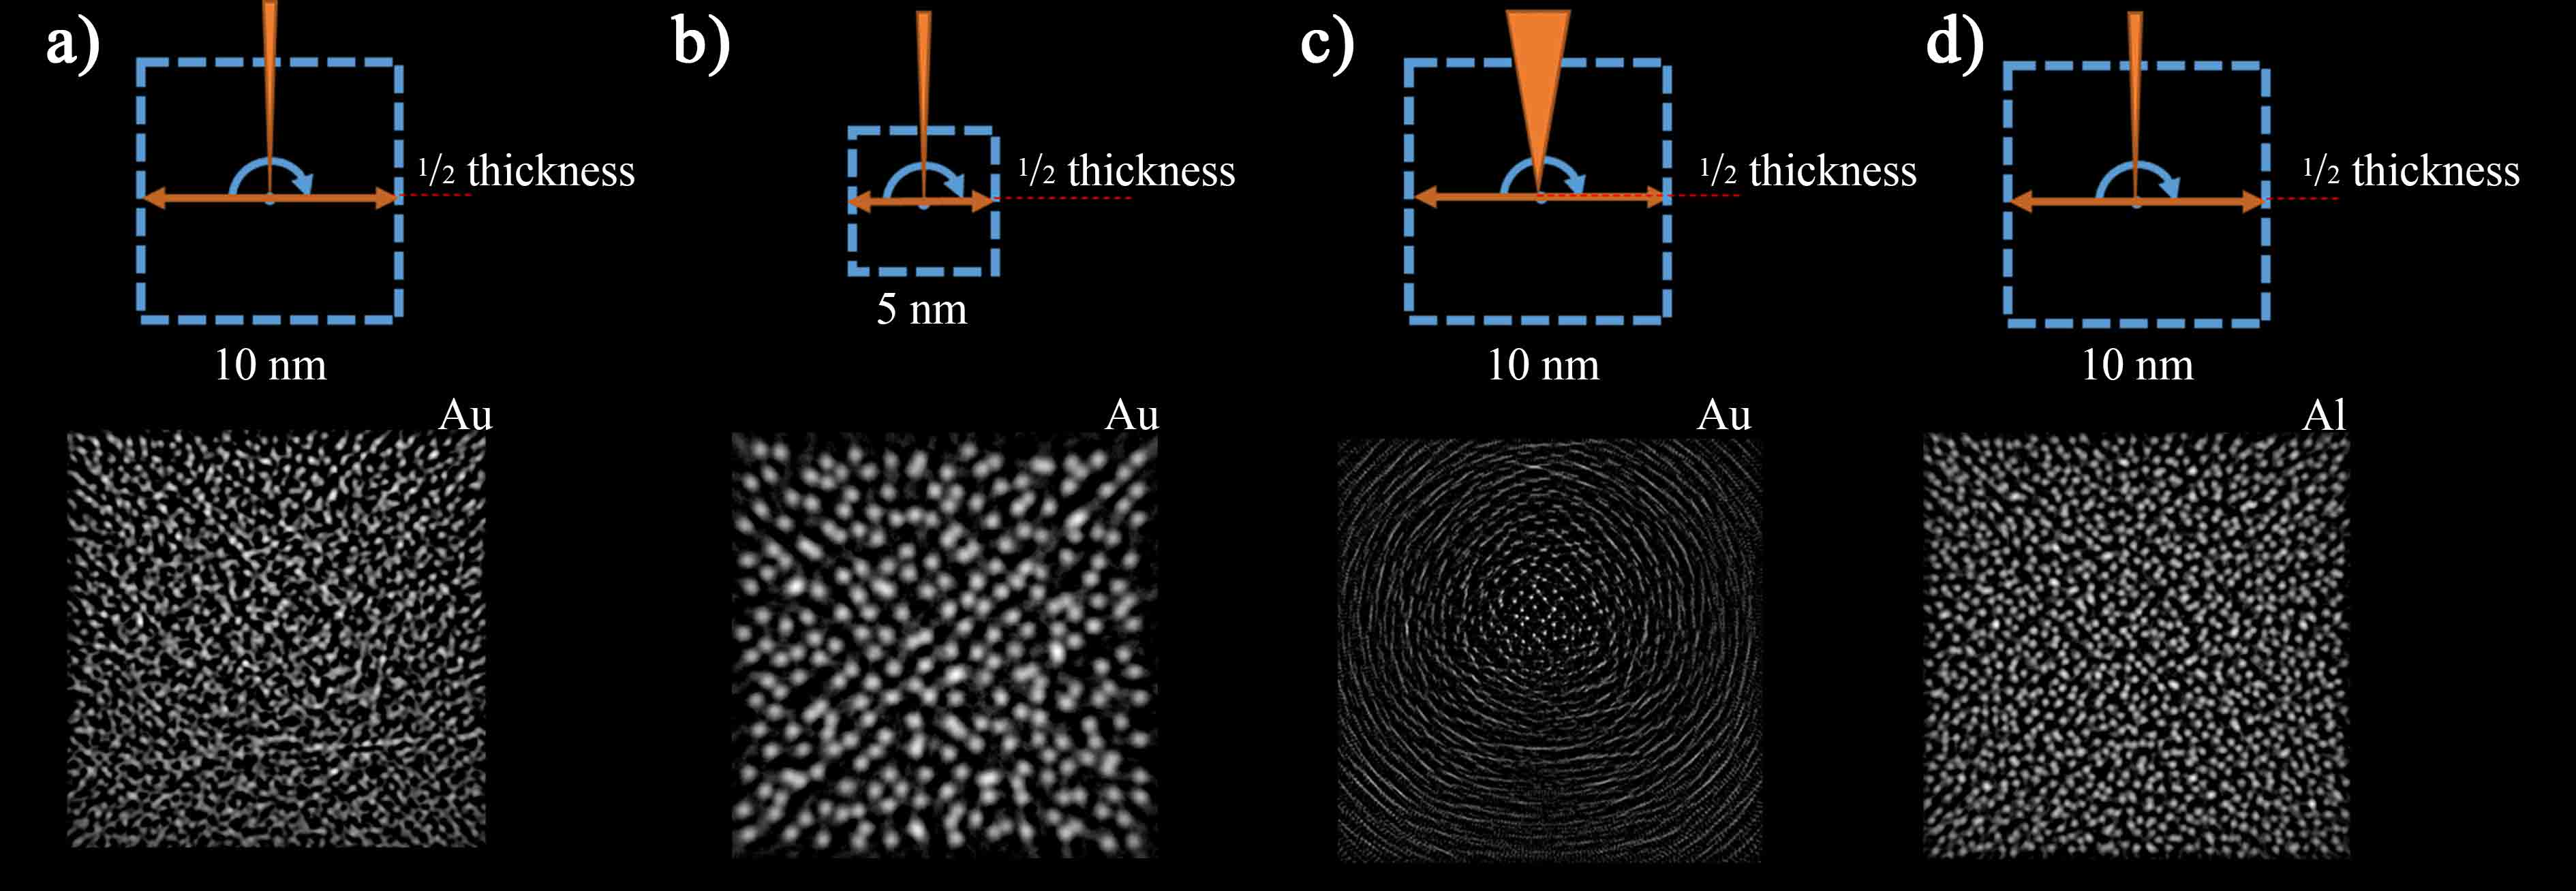
\includegraphics[width=0.85\textwidth]{../4.8/48}
	\caption{影响三维重构的分辨率的因素}\label{fig:48}
	\song\tuzhu{a) 尺寸为 10 nm $\times$ 10 nm $\times$ 2.4 nm 的金原子模型的重构结果。电子束会聚半角为 10 mrad;b) 尺寸为 5 nm $\times$ 5 nm $\times$ 2.4 nm 的金原子模型的重构结果,电子束会聚半角均为 10 mrad;c) 尺寸为 10 nm $\times$ 10 nm $\times$ 2.4 nm 的金原子模型的重构结果,电子束会聚半角均为 50 mrad;d) 尺寸为 的铝原子 $10 \textnormal{ nm}\times10 \textnormal{ nm}\times2.4 \textnormal{ nm}$ 模型的重构结果,电子束会聚半角均为 10 mrad;电子束斑均被聚焦到模型中 1/2 深度,加速电压是 200 kV}
\end{figure}

\section{讨论}
本工作旨在从理论上探究当 STEM 会聚束景深小于样品尺寸时 3DET 重构的可能性,同时揭示其中的特殊现象和规律~\cite{SRH2020}。在理论模拟中,很多现实因素都没有被考虑在内,比如噪音、样品漂移、放大倍数偏离等。会聚束束斑的模拟局限在理想的电镜系统中。比如 R. Xu 等~\cite{Xu2015}成功重构了原子分辨率的尺寸为 10 nm 的钨针尖,但是他们使用的会聚束束斑的会聚半角是 30 mrad,加速电压为 300 kV,其理论景深根据公式(3.3)只有 $1.3\sim4.5$ nm。所以,实际电镜中会聚束的景深,不能简单的根据现有的公式计算得出。



一般情况下,使用低分辨率及低放大倍数的 STEM 图像重构样品的外形时,只要求图像的强度与样品的厚度呈线性关系。然而,原子分辨率的三维重构对 STEM 图像与样品之间的线性关系的要求无疑更为严格。因为STEM 图像实际反映了原子静电势对电子的散射能力,当重构样品中的原子时,实际重构的是原子的静电势分布,所以原子分辨率 3DET 的关键是原子的静电势信息能够线性地被电子束携带并被探测器接收。本章的模拟与重构结果可以反向证明,当 STEM 会聚束束斑的景深小于样品时,STEM 图像的强度反映了样品某一深度内的原子静电势的投影信息,否则不会出现正确重构的区域。 

\begin{figure}[htbp]
	\vspace{\baselineskip}
	\centering
	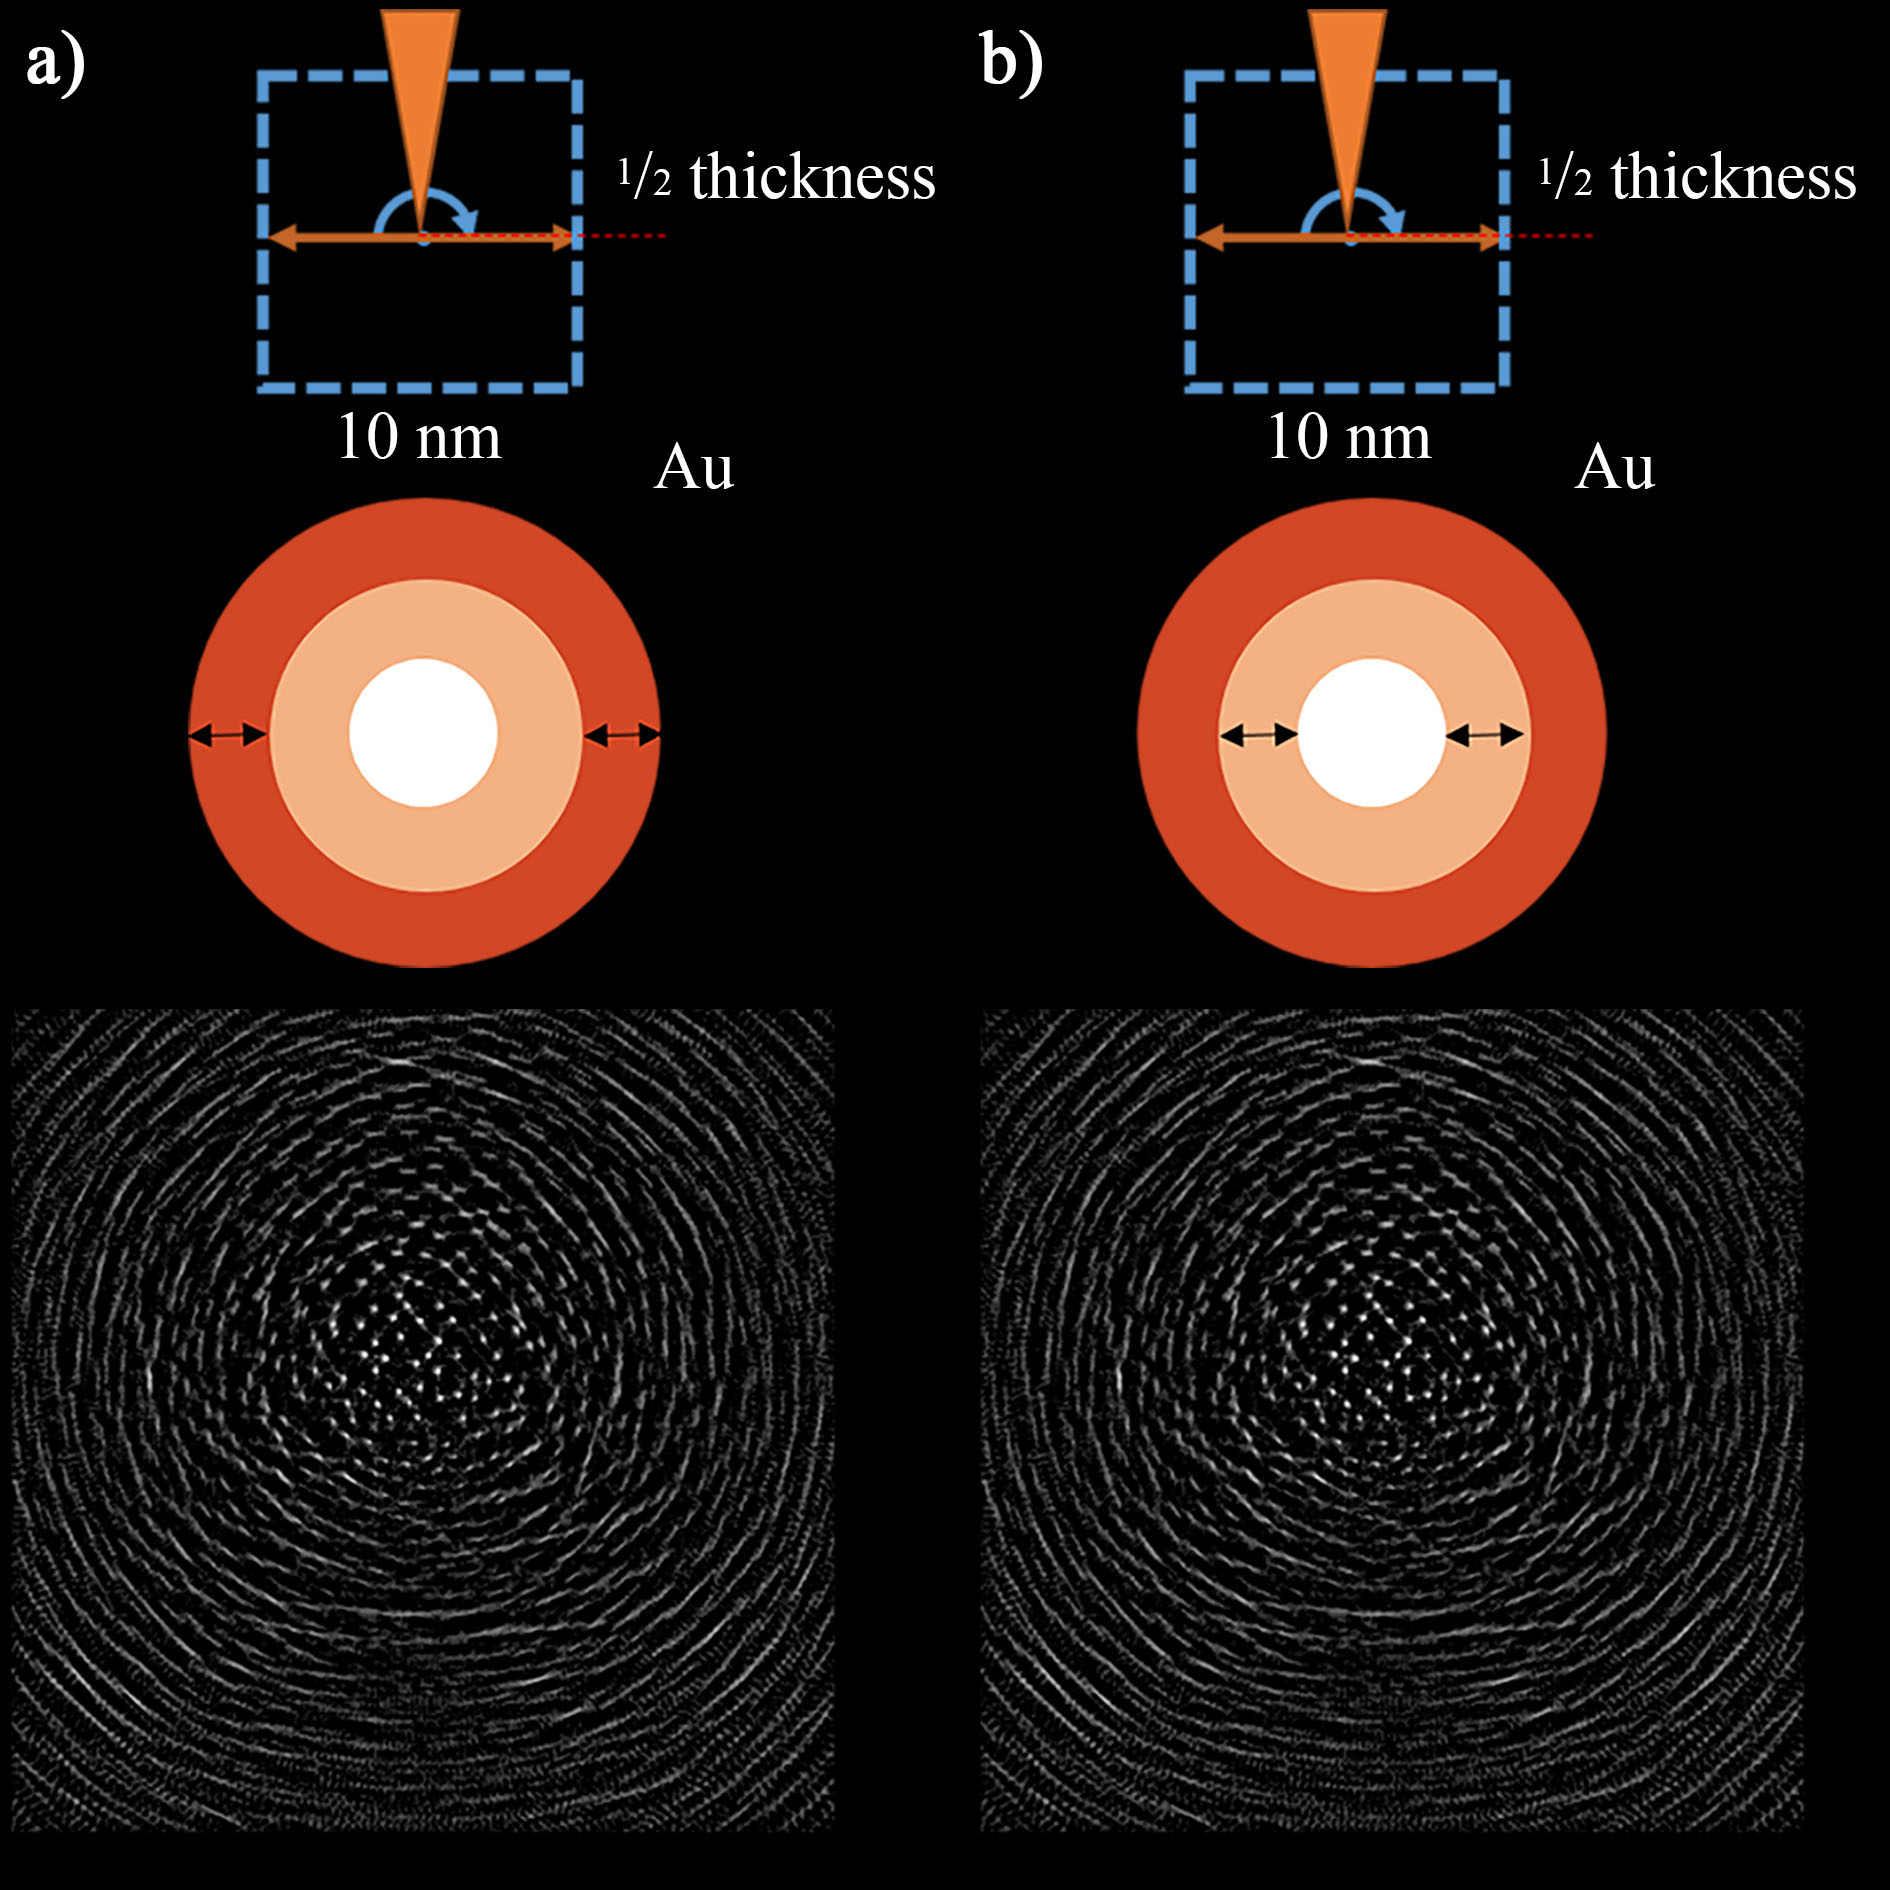
\includegraphics[width=0.9\textwidth]{../4.9/49}
	\caption{尺寸为 10 nm $\times$ 10 nm $\times$ 2.4 nm 的金原子模型在 HAADF 和 ADF 成像模式下的重构结果}\label{fig:49}
	\song\tuzhu{它们的探测器收集角分别为 a) 内角 90 mard,外角 230 mrad,b) 内角 58 mard, 外角 90 mrad;会聚束会聚半角均为 50 mrad,加速电压是 200 kV,会聚束束斑均被会聚到样品厚度 1/2 的深度位置}
\end{figure}

通常认为 HAADF-STEM 图像的的强度与原子序数(Z$^{\sim1.7}$)呈线性关系~\cite{Kubel2005},适合用于 3DET。然而,在 M.C. Scott 等~\cite{Scott2012}和 R. Xu 等~\cite{Xu2015}的研究中使用了 ADF-STEM 倾转系列像成功实现了原子分辨率的三维重构。目前并没有理论能够解释 ADF-STEM 图像与样品之间存在投影关系。图 3.10 通过模拟和重构,比较了 HAADF 和 ADF 两种模式下的重构。图 3.10a 中的 STEM 探测器收集角是 90 mrad $\sim$ 230 mrad,图 3.10b 则为 58 mrad $\sim$ 90 mrad。两个重构的结果没有明显的不同,这个结果支持了上述提到的两个原子分辨率三维重构的成果,说明 ADF-STEM 倾转系列像在一定条件下也可以使用于 3DET,尽管其中还有一些理论问题无法被解释清楚。

另外,图 3.11 对比了不同投影数量和角度范围的重构结果。图 3.11a-c 展示了投影角度为全 180°,但投影角度间隔依次为 1°、2°、3° 时的重构结果。可见,当投影数量减少时,图像的噪音增大,有些原子在重构后会“粘连”,产生重构误差。而图 3.11d-f 展示了投影角度范围为 -80°$\sim$+80°、-70°$\sim$+70°、-60°$\sim$+60° 时的重构结果,即缺失锥逐渐严重。此时,重构的质量也会下降。在第 1.3.8 条中已经论述过,缺失锥假象对重构对象的形貌产生影响,并且假象的严重程度与对象的几何形状有关。在本章论述的问题中,重构的对象是呈点状的原子,所以缺失锥假象对重构的影响是有限的,特别是重构的实质信息仅是原子的位置,而非形状。所以,在一般的透射电镜中开展实验时,缺失锥问题不应当是影响重构的重要因素。而投影数量的整体减少,却可与实验噪音共同对重构造成较大影响。


\begin{figure}[htbp]
	\vspace{\baselineskip}
	\centering
	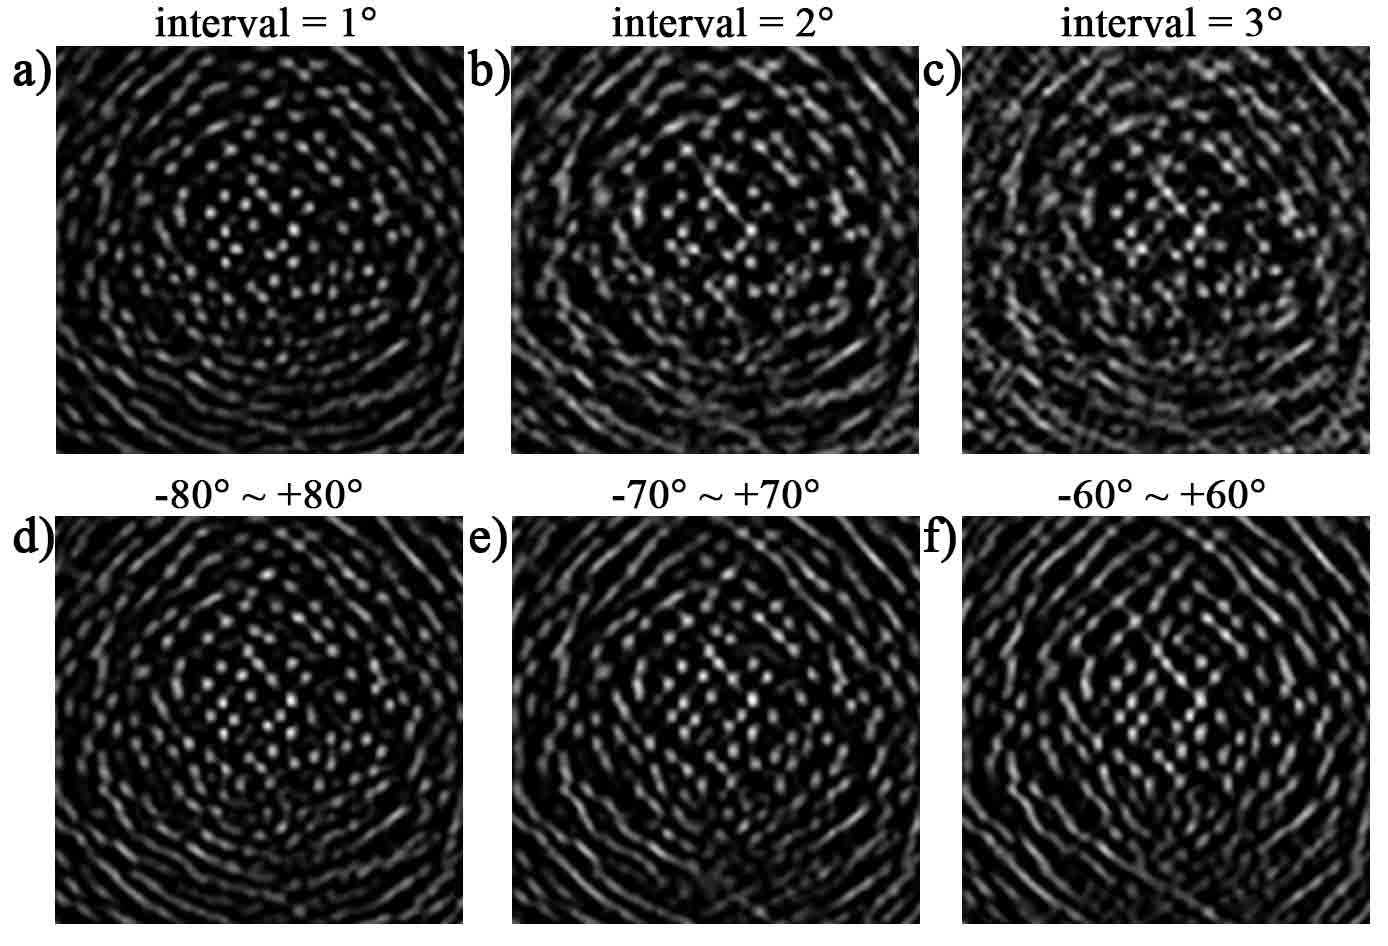
\includegraphics[width=0.9\textwidth]{../4.12/412}
	\caption{投影数量和角度范围对重构的影响}\label{fig:412}
	\song\tuzhu{a) 投影角度是全 180°,角度间隔为 1°;b)  投影角度是全 180°,角度间隔为 2°;c)  投影角度是全 180°,角度间隔为 3°;d)  投影角度是全 -80°$\sim$+80°,角度间隔为 1°;e)  投影角度是全 -70°~+70°,角度间隔为 1°;f)  投影角度是全 -60°~+60°,角度间隔为 1°;模拟参数见图 3.10a,图像取了整图的局部}
\end{figure}


一般的块体材料的三维重构要求 HAADF-STEM 信号反映物体的质厚投影,分辨率较低。HAADF-STEM 信号的本质来源是原子核与电子之间的卢瑟福散射,反映的是原子对电子的散射能力,当讨论问题达到原子分辨率时,我们才逐渐开始讨论到该本质问题,即 HAADF-STEM 的信号强度与这种散射能力之间是否具有良好的线性关系。答案是肯定的,因为 HAADF-STEM 倾转系列像的 tomography 重构结果能够清晰地反映出原子所在的位置,即其重构的原子对电子散射能力在空间中的分布是符合理论预期的。并且,原子的静电势对电子束的汇聚作用在这种情况下也对重构结果产生影响。所以才出现了与重构块体材料时不同的现象。

\section{本章小结}
本章通过理论模拟,探究了景深对三维重构的影响。当 STEM 入射电子束的景深达到纳米尺度,小于样品的厚度时,HAADF-STEM 像仍然可用于 tomography 三维重构。但此时只有样品内部局部区域的原子能被正确地重构。

正确重构的区域位置、厚度以及重构的质量,和入射电子束斑的会聚半角、加速电压、聚焦位置以及其与倾转轴的相对位置有关。保证电子束斑聚焦在与倾转轴同一样品深度,能够最大程度地获得高质量的重构结果。此外,因重元素原子静电势对电子束的作用而带来的提前聚焦现象会干扰对电子束实际束斑位置的精确控制。

要保证足够的三维重构分辨率以分辨原子,不仅要考虑电子束的分辨率与景深,还要考虑样品厚度和样品的元素的影响。尺寸大且内部原子属于重元素的样品较难重构,应尽量选择较大的会聚半角和较高的加速电压;小尺寸、轻元素的样品更容易达到高分辨率的三维重构,所以可以适当选择较小的会聚半角和低加速电压,以获得更大的重构区域。要获得理想的原子分辨率三维重构,需要综合考量分辨率、景深、样品厚度和样品元素等因素对重构结果的影响。

本工作在理论上揭示了原子分辨率的三维重构与一般块体材料的三维重构的差别,对实验具有指导意义。



% !Mode:: "TeX:UTF-8"

\clearemptydoublepage

\chapter[一种从单张 TEM 原子像测量晶体三维形貌的方法]{一种从单张 TEM 原子像测量晶体\\三维形貌的方法}

\section{引言}

自 20 世纪 70 年代以来,根据材料的二维投影图像重构其内部三维结构信息的技术一直是研究热点~\cite{DeRosier1968},它被广泛应用于化学、生物医药、工业等领域。三维重构是研究材料的重要手段,这是因为材料的宏观性能由其三维微观结构所决定,仅知其二维投影结构不足以准确推断其宏观性能。比如,纳米颗粒的整体以及表面的三维形态对其自身的催化性能具有至关重要的决定作用~\cite{Jaramillo2007};在传统合金材料铝合金中,铝基体内部的纳米析出相的三维形状、尺寸及分布,对其宏观力学性能具有重大影响~\cite{Chen2006,Yang2014,Malladi2014}。三维重构技术为材料科学家们提供了便利的手段,使他们能够通过有限数量的二维投影重构材料的三维结构信息。

在透射电子显微学中,有几种从二维投影重建材料三维结构的方法,例如倾转系列 3DET~\cite{Kubel2005,Xu2015,Scott2012,Miao2005,Mao2010,Lu2015},光学层析法~\cite{Xin2009,Intaraprasonk2008,Xin2008,Borisevich2006,Yang2015,VandenBroek2010},以及一类新开发的基于定量分析二维高分辨 TEM 照片或出射面波函数进行三维重构的方法~\cite{ChenFR2017,ChenFR2016,Jia2014,VanDyck2012,ChenFR2015,WangA2012,WangA2010}。倾转系列 3DET 是使用最为频繁和广泛的三维重构方法,一直以来,该方法在理论和实验上都不断地取得突破,许多令人兴奋的研究成果踊跃而出~\cite{Zhou2019,Xu2015,Scott2012,Lu2015}。尽管如此,该方法在实际使用中依然要面对不少困难,比如缺失锥,电子辐照损伤,样品漂移等问题。光学层析方法则依据材料的欠焦系列 STEM 照片重构其三维形貌。使用该方法的前提是假定每一张二维 STEM 照片的信息对应于材料某一深度片层内的结构信息。然而,聚光镜光阑的尺寸严重限制了电子束斑在 $z$ 方向上的分辨率,使得光学层析在实际应用中受限。而且,由于长时间的图像收集操作,该方法同样易受电子辐照损伤和样品漂移的影响。目前为止,缺失锥、电子辐照损伤、样品漂移、聚光镜光阑大小依然是限制这两种三维重构方法成像质量和分辨率的主要因素。

最近,有研究者提出了一类新的原子分辨率三维重构方法,这类方法仅需极少数二维实验投影图像,就能在原子分辨率下重构材料的三维结构。例如,结合离散三维重构和原子计数技术~\cite{Alania2017,Lefebvre2015},S. Van Aert 等通过两张原子分辨率 STEM 照片重构了嵌入于铝基体中的纳米银颗粒内部的原子排列~\cite{VanAert2011}。D. Van Dyck 等使用 “Big Bang” 三维重构技术重构了双层石墨烯的三维原子排列~\cite{VanDyck2012}。该方法通过对出射面波函数的相位与一个已知量 “phase speed” 进行线性拟合,推测石墨烯样品中的原子在 $z$ 方向上的位置。类似的,F.R. Chen 等提出一种三维全息方法~\cite{ChenFR2017,ChenFR2016},该方法根据通道理论,利用出射面波函数的实部与虚部之间的关系来分析样品中每一个原子柱包含的原子个数以及这些原子在 $z$ 方向上的位置。后两种方法中的出射面波函数通常由 10 到 20 张欠焦系列 TEM 照片重构得到,在拍摄这些照片的过程中,电子辐照损伤和样品漂移依然不可避免。

值得注意的是,在对球差矫正 TEM 最佳成像机制的早期研究中,J.H. Chen 等通过对比实验与模拟图像的衬度,从一张正带轴的 Si 的原子分辨率二维 TEM 照片,推测出了样品的三维楔形形状~\cite{Chen2004}。在这个研究中,图像中的原子柱在 $x-y$ 平面的位置可以直接根据图像确定,所以只需要通过衬度分析推测每个原子柱的厚度和欠焦量,就可以确定样品的三维结构。不过,这种半定量的分析手段精确程度不高,而且例如 MTF 对图象衬度的影响等诸多因素都没有被正确地考虑。令人兴奋的是,2014 年,C.L. Jia 等通过一张二维的高分辨 TEM 照片,在原子分辨率下重构了纳米 MgO 晶体的表面形貌。在他们的重构方法中,电镜照片中的每一个原子柱位置的图像强度都被定量地与模拟图像进行对比,这是一种崭新的基于定量分析球差矫正高分辨 TEM 照片的原子分辨率三维重构方法。该研究中的电镜照片是使用 NCSI 技术拍摄得到,且解理的 MgO 晶体周围没有非晶覆盖,成像质量非常高,这在一般电镜实验中是难以达到的。而且,该方法通过对比原子柱处的图像强度来分析样品的三维结构,所以该方法要求图像衬度与原子结构之间具有很高的线性关系。

然而,在一般的高分辨 TEM 成像实验中,非晶对图像衬度的影响是不可忽略的,而且原子柱之间互相影响的衬度信息也往往不可避免。此外,目前还没有明确的方法定义这种定量三维重构方法的分辨率。这些问题的存在限制了该方法的广泛使用。本章通过模拟和实验探究,更加细致地讨论了这些问题。

在本章中,我们首先提出了一种自洽性验证的重构方法,它通过定量分析整张二维图像的图像强度来重构一般晶体材料表面的三维原子结构~\cite{SRH2019}。同时,该方法还能够估计和定义三维重构的分辨率,引入置信度来定量探究非晶对重构结果的影响。我们使用该方法重构了 Si[110] 晶体样品的二维原子分辨率 TEM 照片,并且测得该重构的结果在原子柱的高度(欠焦量)和厚度(原子个数)方面的分辨率都是一个原子间距(= 0.384 nm),其表面覆盖的非晶层厚度小于 1 nm。

\section{全局匹配算法及模拟测试}
\subsection{算法介绍}
根据单张二维高分辨率 TEM 原子像进行三维重构的基本原理是,通过定量比较模拟像与实验像的图像强度,并不断改变样品模型和模拟的参数进行高分辨 TEM 照片模拟,寻找最佳的模型与成像参数,例如欠焦量、样品厚度、样品倾转等。对于一张一般的高分辨 TEM 照片而言,在整个成像过程中未知的参数太多,在诸多参数之间优化找到全局最佳是不切实际的。幸运的是,球差矫正 TEM 可以矫正大部分像差,这使得上述三维重构问题中待优化的参数极大减少,从而使得该定量匹配方法变得切实可行。不过,现阶段要实现重构,依然需要对待重构的样品做一定的假设,它应该满足以下四个前提条件:(1)样品必须是晶体,且其块体结构已知;(2)二维实验图像必须具有原子分辨率,样品中的每一个原子柱在 $x-y$ 平面上的位置,可以通过实验照片直接测量得到;(3)样品中的杂质、缺陷、畸变可以被忽略;(4)在电镜照片的拍摄过程中,样品被精确地倾转至正带轴。如此,样品的三维形貌就仅由每个原子柱的厚度(原子个数)和高度(欠焦量)决定,这使得原子分辨率的定量分析三维重构实际可行。

在优化过程中,一个好的初始模型对取得正确的优化结果具有重要意义。对于本章所研究的三维重构而言,我们可以从一个平整的样品模型(即模型中原子柱的厚度均相等)开始优化。模型的上下表面可以是倾斜的(原子柱的欠焦量线性变化),也可以不倾斜。

在整个重构方案中,最耗时的过程是从初始模型开始,通过全局匹配算法优化模型上下表面的原子结构。该算法将不断地调整模型的原子结构并模拟该模型的高分辨 TEM 照片,将得到的模拟像与整张实验像进行定量强度对比。其中图像模拟使用多片层法~\cite{Chen1995,Chen1997,Chen1997-1,Chen1995-1,Chen1997-2},该方法可以计算动力学电子散射,包括部分相干成像的透射交叉系数理论~\cite{Chen2004,Ishizuka1980,Frank1973}。由于全局匹配算法相比于局部匹配算法耗时更多,所以我们的算法使用了热门的 compute unified device architecture (CUDA)语言和图形处理单元(graphic processing unit , GPU)加速技术~\cite{Garland2008}。

为了说明在定量图像强度匹配的原子分辨率三维重构中使用全局匹配算法的必要性,我们通过模拟测试对比了全局匹配和局部匹配这两种算法的重构结果。图 1a 展示了模拟所使用的 Si[110] 模型。该模型中的所有原子柱的厚度均是 3.84 nm,它的表面沿 $y$ 方向倾斜。电子束($z$ 方向)沿 Si[110] 方向入射。图 4.1a 中垂直于 $z$ 方向的粉色平面是零欠焦面,它是欠焦量和原子柱高度的坐标原点。表 4.1 详细展示了像模拟时使用的参数。使用这些参数对该模型进行像模拟之后,得到的 TEM 模拟像将被当作实验图像,并分别使用两种重构算法对其进行重构。在全局匹配算法中使用的初始模型是表面平整的超胞模型。值得注意的是,在优化和定量对比的过程中,在模拟之前,需要在原子模型周围加入一定量的真空,以避免环绕效应。$\textnormal{图 1d}$ 展示了 Si[110] 模型的 $x-y$ 平面投影结构。为了方便讨论,图 4.1e 展示了 Si[110] 的单胞。


\begin{figure}[htbp]
	\vspace{\baselineskip}
	\centering
	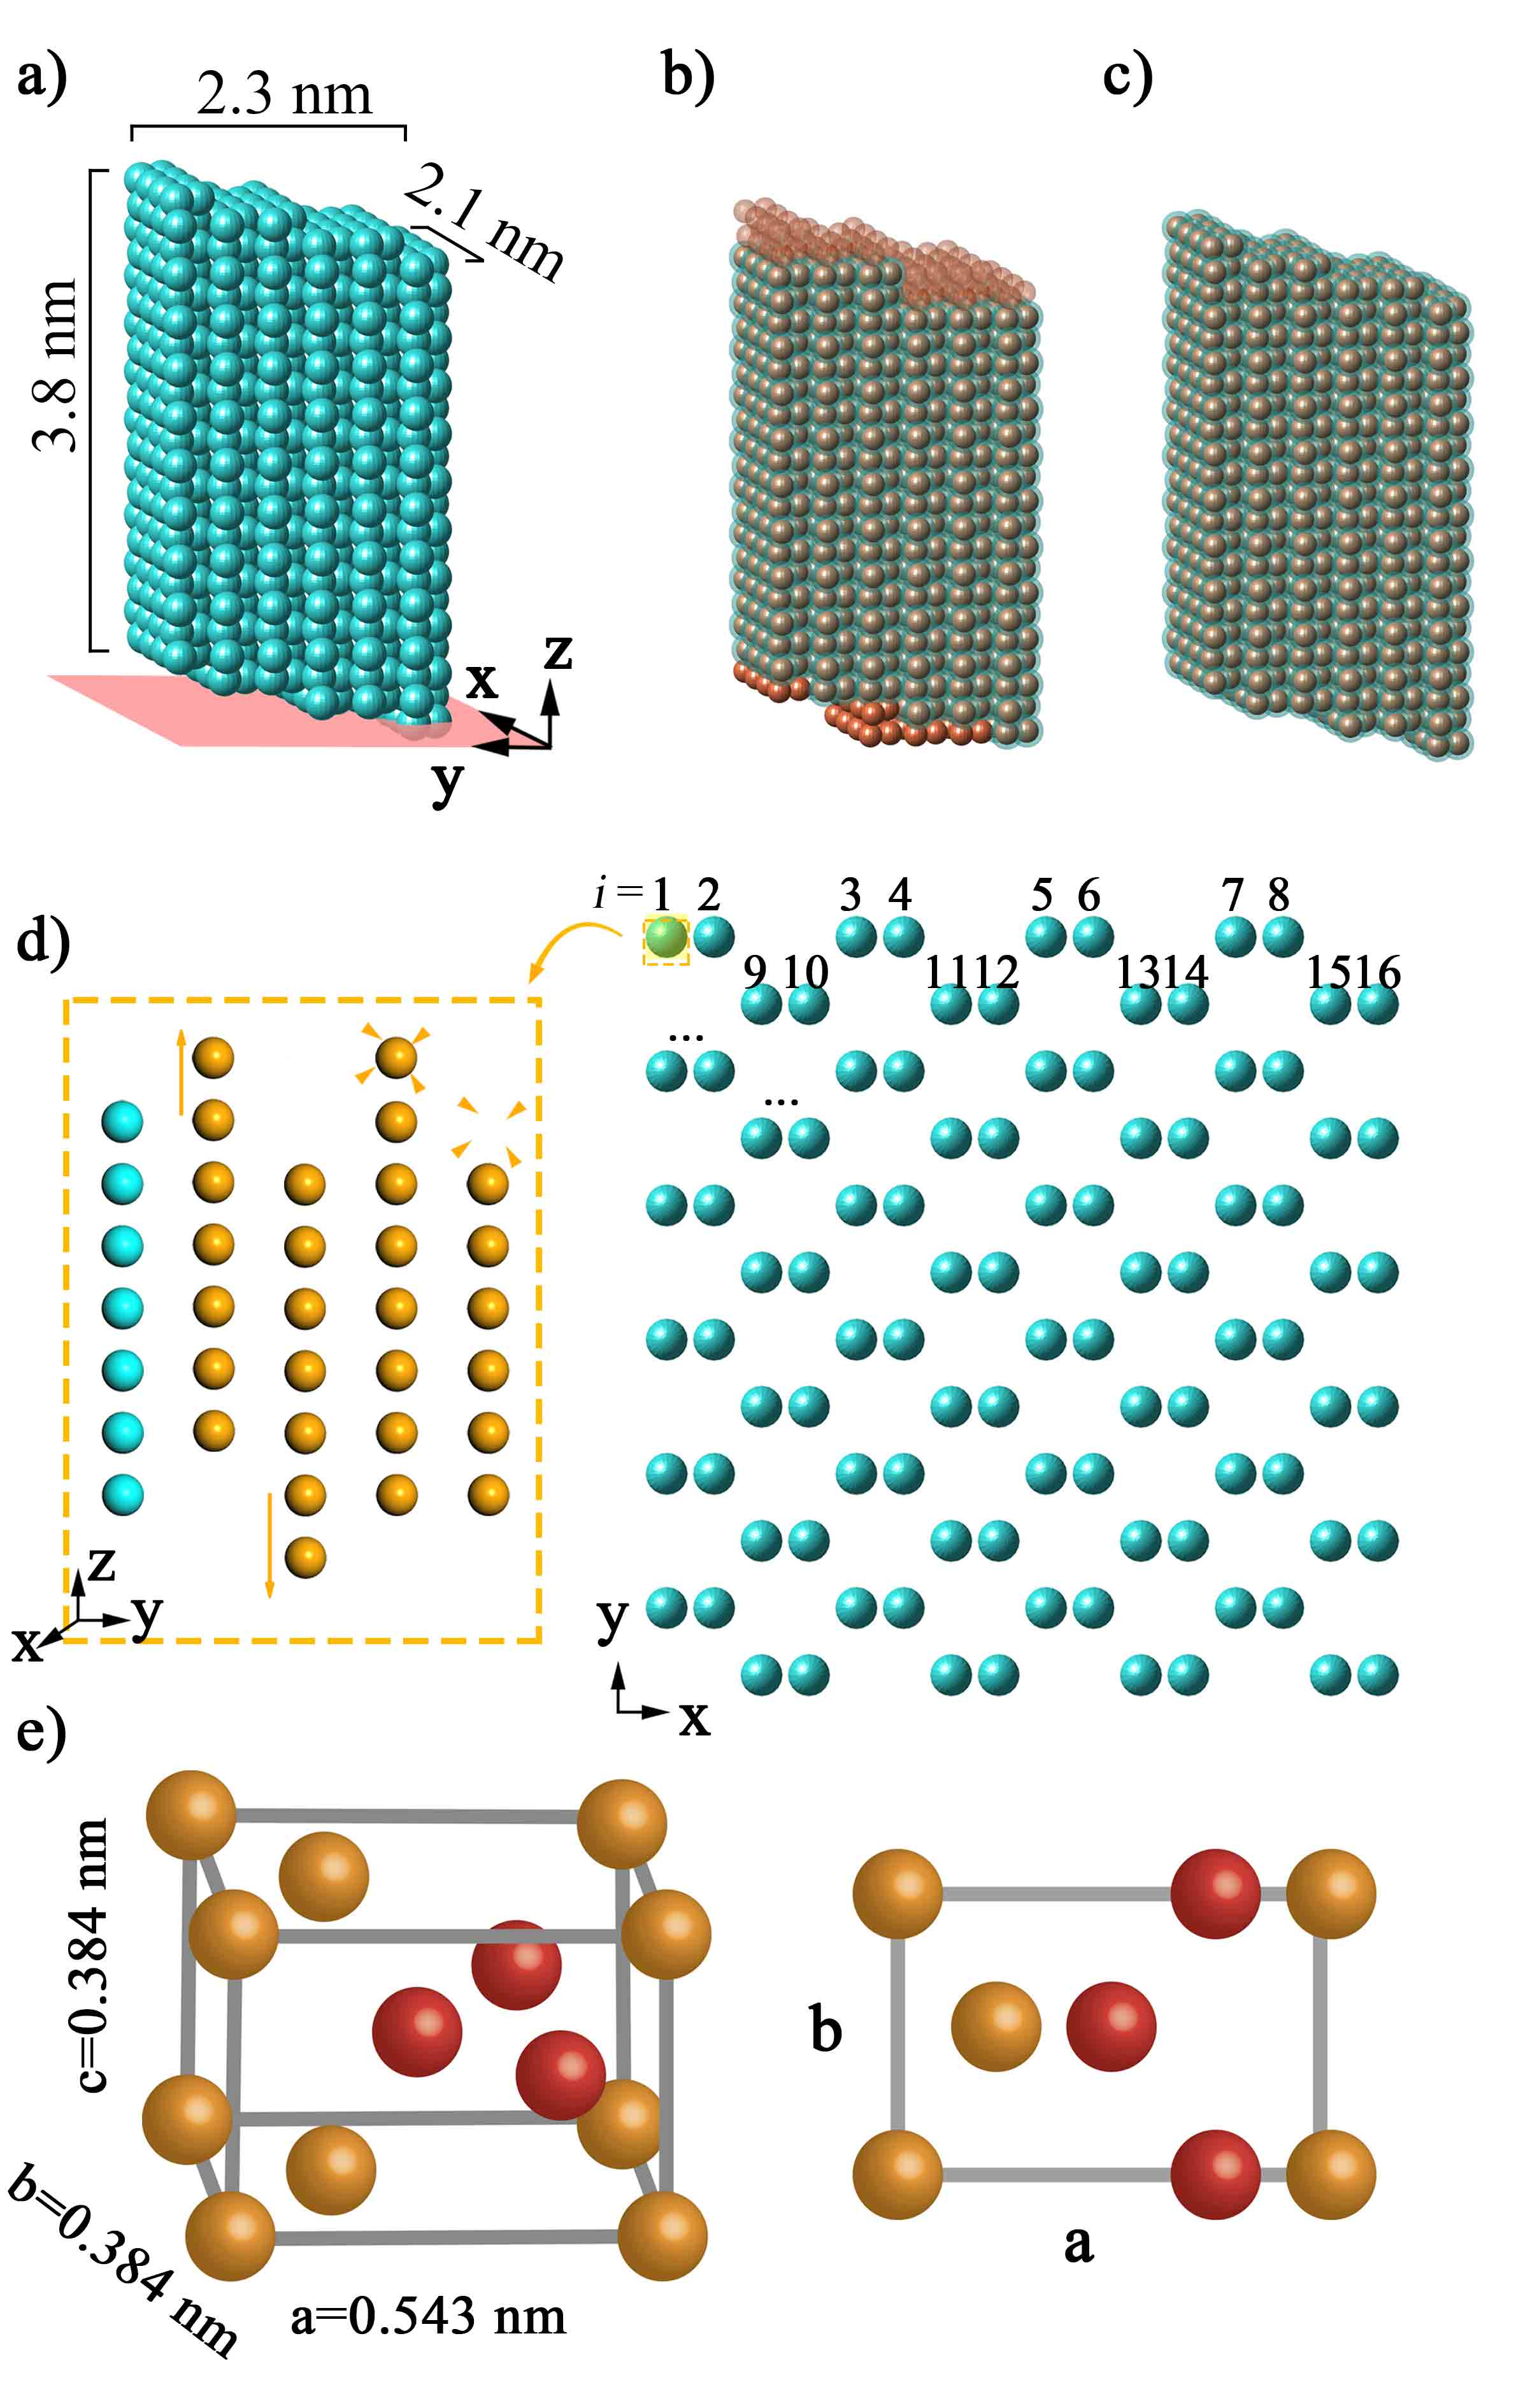
\includegraphics[width=0.8\textwidth]{../2.1/21}
	\caption{模拟测试的示意图}\label{fig:21}
	\song\tuzhu{a) 模拟测试使用的 Si[110] 样品模型的三维形貌图,该模型的上下表面具有一定的倾斜;其中 $x$,$y$,$z$ 轴分别对应 [111],[001],[110] 方向;垂直于 $z$ 轴的粉色平面是零欠焦面;b) 局部匹配算法的重构结果,其表面的一些原子(棕色表示)是错误的,透明棕色表示这些原子没有被正确重构出来;c) 全局匹配算法的重构结果,其与原始模型a)完全一致;d) Si 模型的顶视图,其左边的插图描述了各原子柱在优化时将在厚度(原子柱中的原子个数)和高度(欠焦量)上被调整;每个原子柱在优化时被标记为 $i$ ($i = 1,2, \cdots, N$);e) 左边是 Si[110] 的单胞三维图像,$c$ 平行于 [110];右边是该单胞的顶视图;单胞中橙色的原子处于 $z = 0$ 的位置,而红色的原子处于 $z = 0.5c$ 的位置}
\end{figure}
图 4.1b 是局部匹配算法的重构结果。在这个方法中,整个“实验”图像将以单胞为单位被分割成若干部分。图像的模拟和对比仅分别针对每一个分割出的图像,以确定该图像所对应的原子柱的厚度和欠焦量。从图 4.1b 可知,局部匹配算法所重构的结果相对于原始的结构模型存在明显的误差。尽管如此,它能够合理地反映出原始的原子模型的表面是存在某种程度的倾斜的。图 4.1c 展示了全局匹配算法的重构结果。可以发现,全局匹配算法重构的原子模型与原始模型完全一致,不存在任何误差。

图 4.2 展示了算法的流程图,每当某一 Si 原子柱 $i$($i = 1, 2 \cdots N, N = 96$, 如图 4.1d 所示)发生改变时,整个模型的模拟图像将与实验图像进行对比,对比结果以绝对误差 $D$ 作为评判标准,以优化该原子柱的厚度和高度。所有 $N$ 个 Si 原子柱将被不断地调整优化直到整个模型不再发生任何变化。

\begin{equation}
D=\sum_{i=1}^N \left(\left|I_n-I_n^{exp}\right|\right)/N_{pixel}
\end{equation}

\begin{figure}[htbp]
	\vspace{\baselineskip}
	\centering
	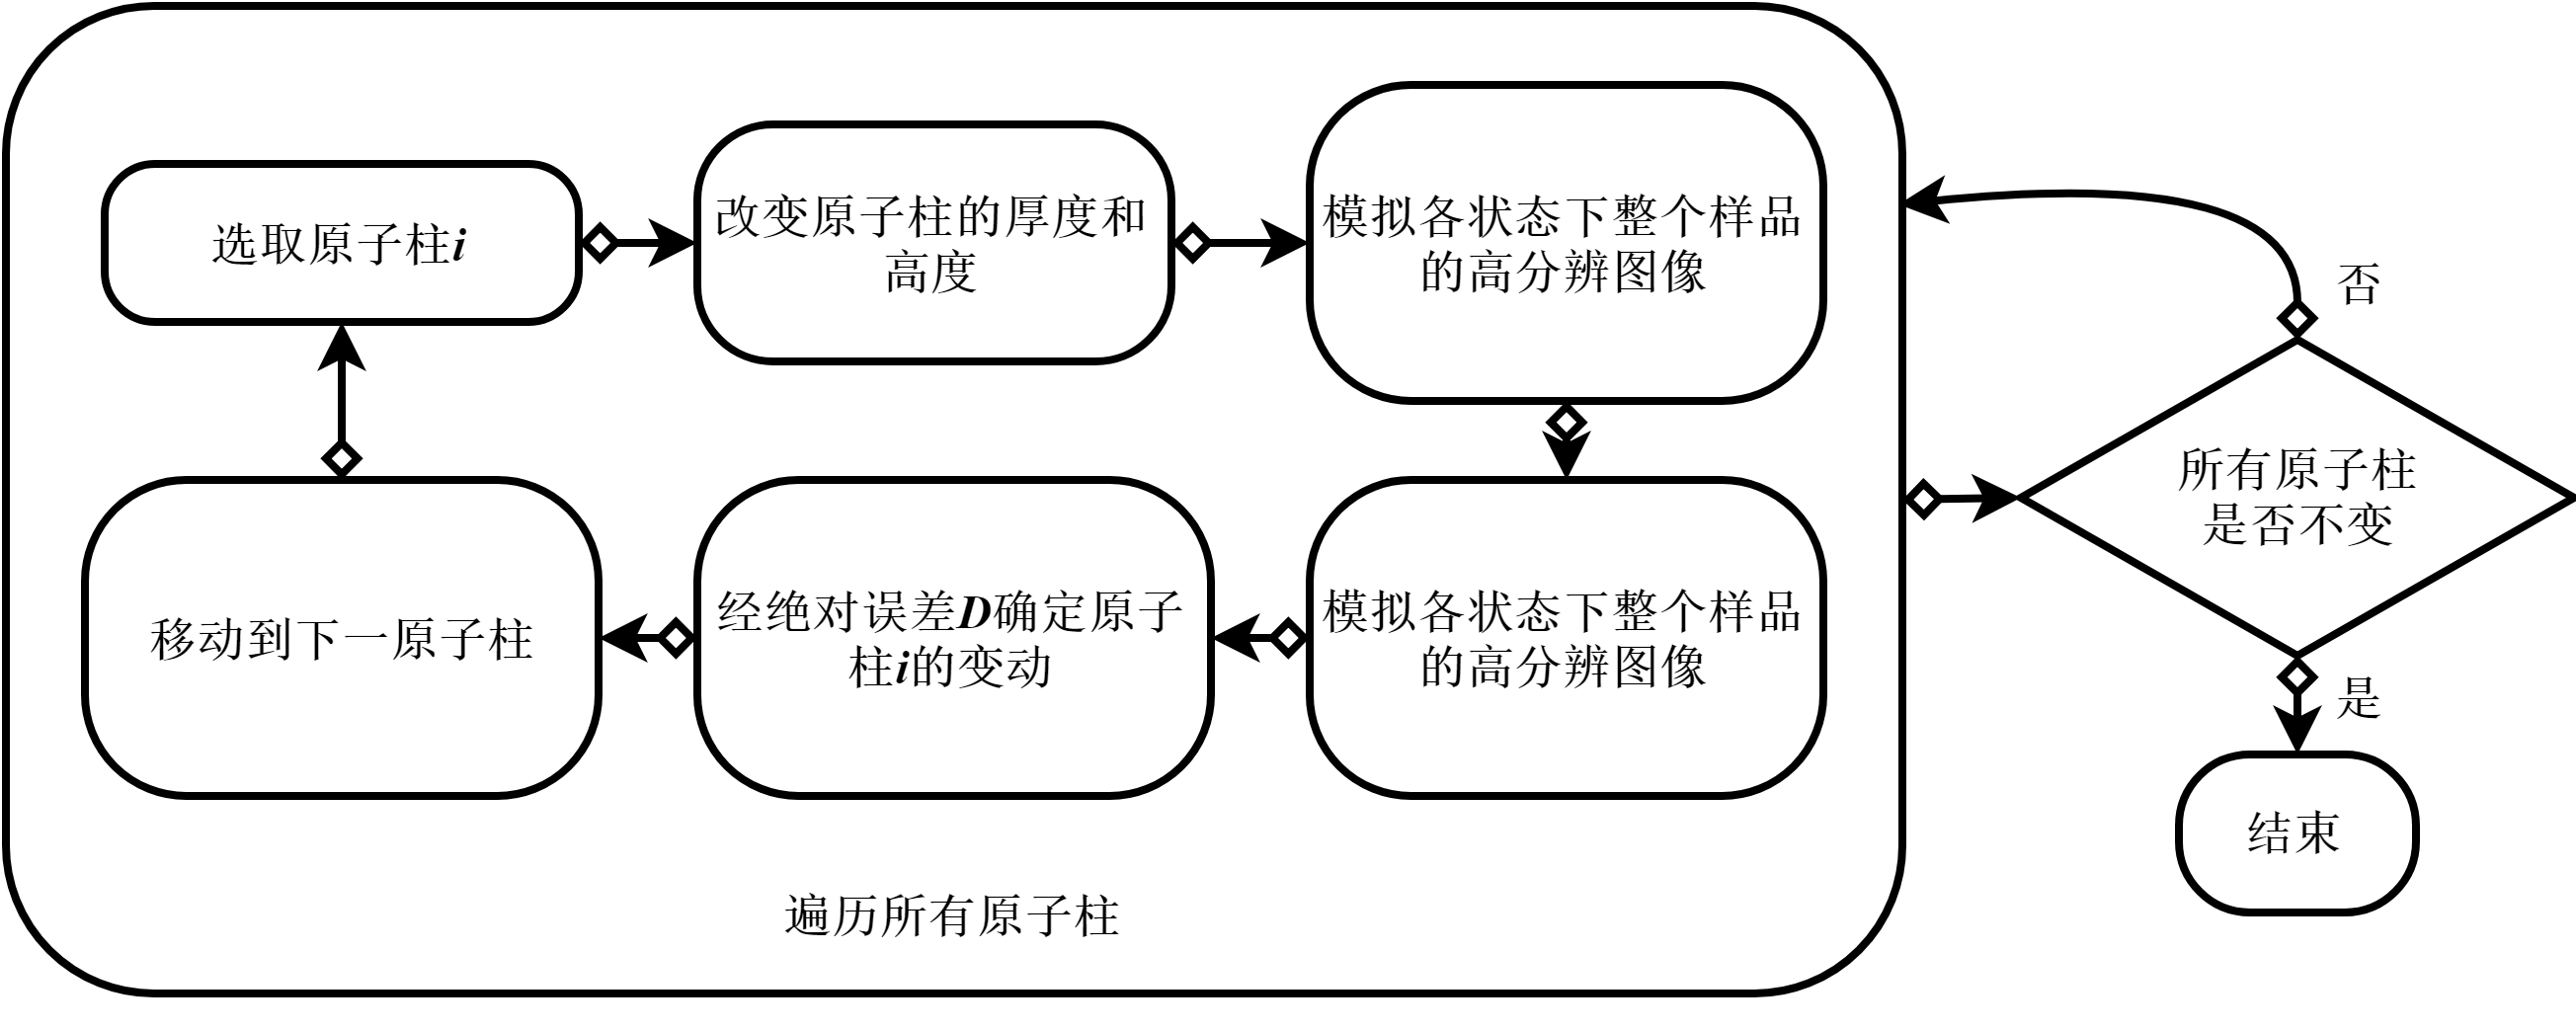
\includegraphics[width=0.8\textwidth]{../2.20/220}
	\caption{算法流程图}\label{fig:220}
\end{figure}

\quad

全局匹配算法的重构结果更加准确的原因主要分为两个方面:首先,全局匹配算法可以避免环绕效应。再者,该方法考虑了包括离域效应在内的所有非线性成像效应。一般来说,由于非线性成像效应,某一原子柱在成像时会影响其周围原子柱的图像衬度。尽管这种效应在原子成像条件下可以被降低到最小,但是不可能被完全消除。因此,在一般的三维重构中,为了达到原子分辨率的重构,应该优先考虑使用全局匹配算法进行重构,而局部匹配算法可以用来重构一个粗略模型为全局匹配算法提供合理的初始模型。

\quad

\begin{table}[htbp]
	\caption{图像模拟参数}\label{tab:table1}
	\vspace{0.5em}\centering\wuhao
	\begin{tabular}{cccc}
		\toprule[1.5pt]
		Parameters & Magnitude\\
		\midrule[1pt]
		Cs$_3$ & 0.015 mm & \\
		Defocus & -3 nm \\
		\quad\quad\quad\quad\quad Semi-Convergence angle\qquad\quad\quad\quad\quad & \quad\quad\quad\quad\quad0.25 mrad\qquad\quad\quad\quad\quad \\
		Objective aperuture & 0.7 $\mathring{A}^{-1}$ \\
		Focus spread & 47 $\mathring{A}$ \\
		Debye-Waller factor & 0.5 $\mathring{A}^2$ \\
		\bottomrule[1.5pt]
	\end{tabular}
	\vspace{\baselineskip}
\end{table}

\subsection{模拟测试方案}
本条将通过重构模拟的高分辨像来测试全局匹配算法。为此构造了如图 4.3a 所示的两个超胞,s1 和 s2。这两个超胞的表面均是倾斜的,这将引起成像的梯度欠焦。且它们的厚度和表面的倾斜程度均不相同,以此作为对比。更详细的超胞信息和模拟参数见图 4.3 和表 4.3。为了避免环绕效应,超胞的左右两端需要加入真空层,并以图 4.3c 中的区域作为重构的感兴趣区域。重构完成后,重构的结果将与正确的超胞进行对比,统计每一个原子柱厚度和高度的误差,并根据公式(4.2)和公式(4.3)计算出平均误差和最大绝对误差:
\begin{equation}
\text{average error} = \sum_{n=1}^N \frac{\left|c_n^{\prime}-c_n\right|}{N}
\end{equation}
其中 $n$ 表示某一原子柱,$N$ 是原子柱的总数,$c_n^{\prime}$ 表示重构的原子柱 $n$ 的厚度或高度,$c_n$ 表示原始超胞中的原子柱 $n$ 的厚度或高度。
\begin{equation}
\text{max absolute error}=\max \left(\left|c_n^{\prime}-c_n\right|\right)
\end{equation}
\begin{figure}[htbp]
	\vspace{\baselineskip}
	\centering
	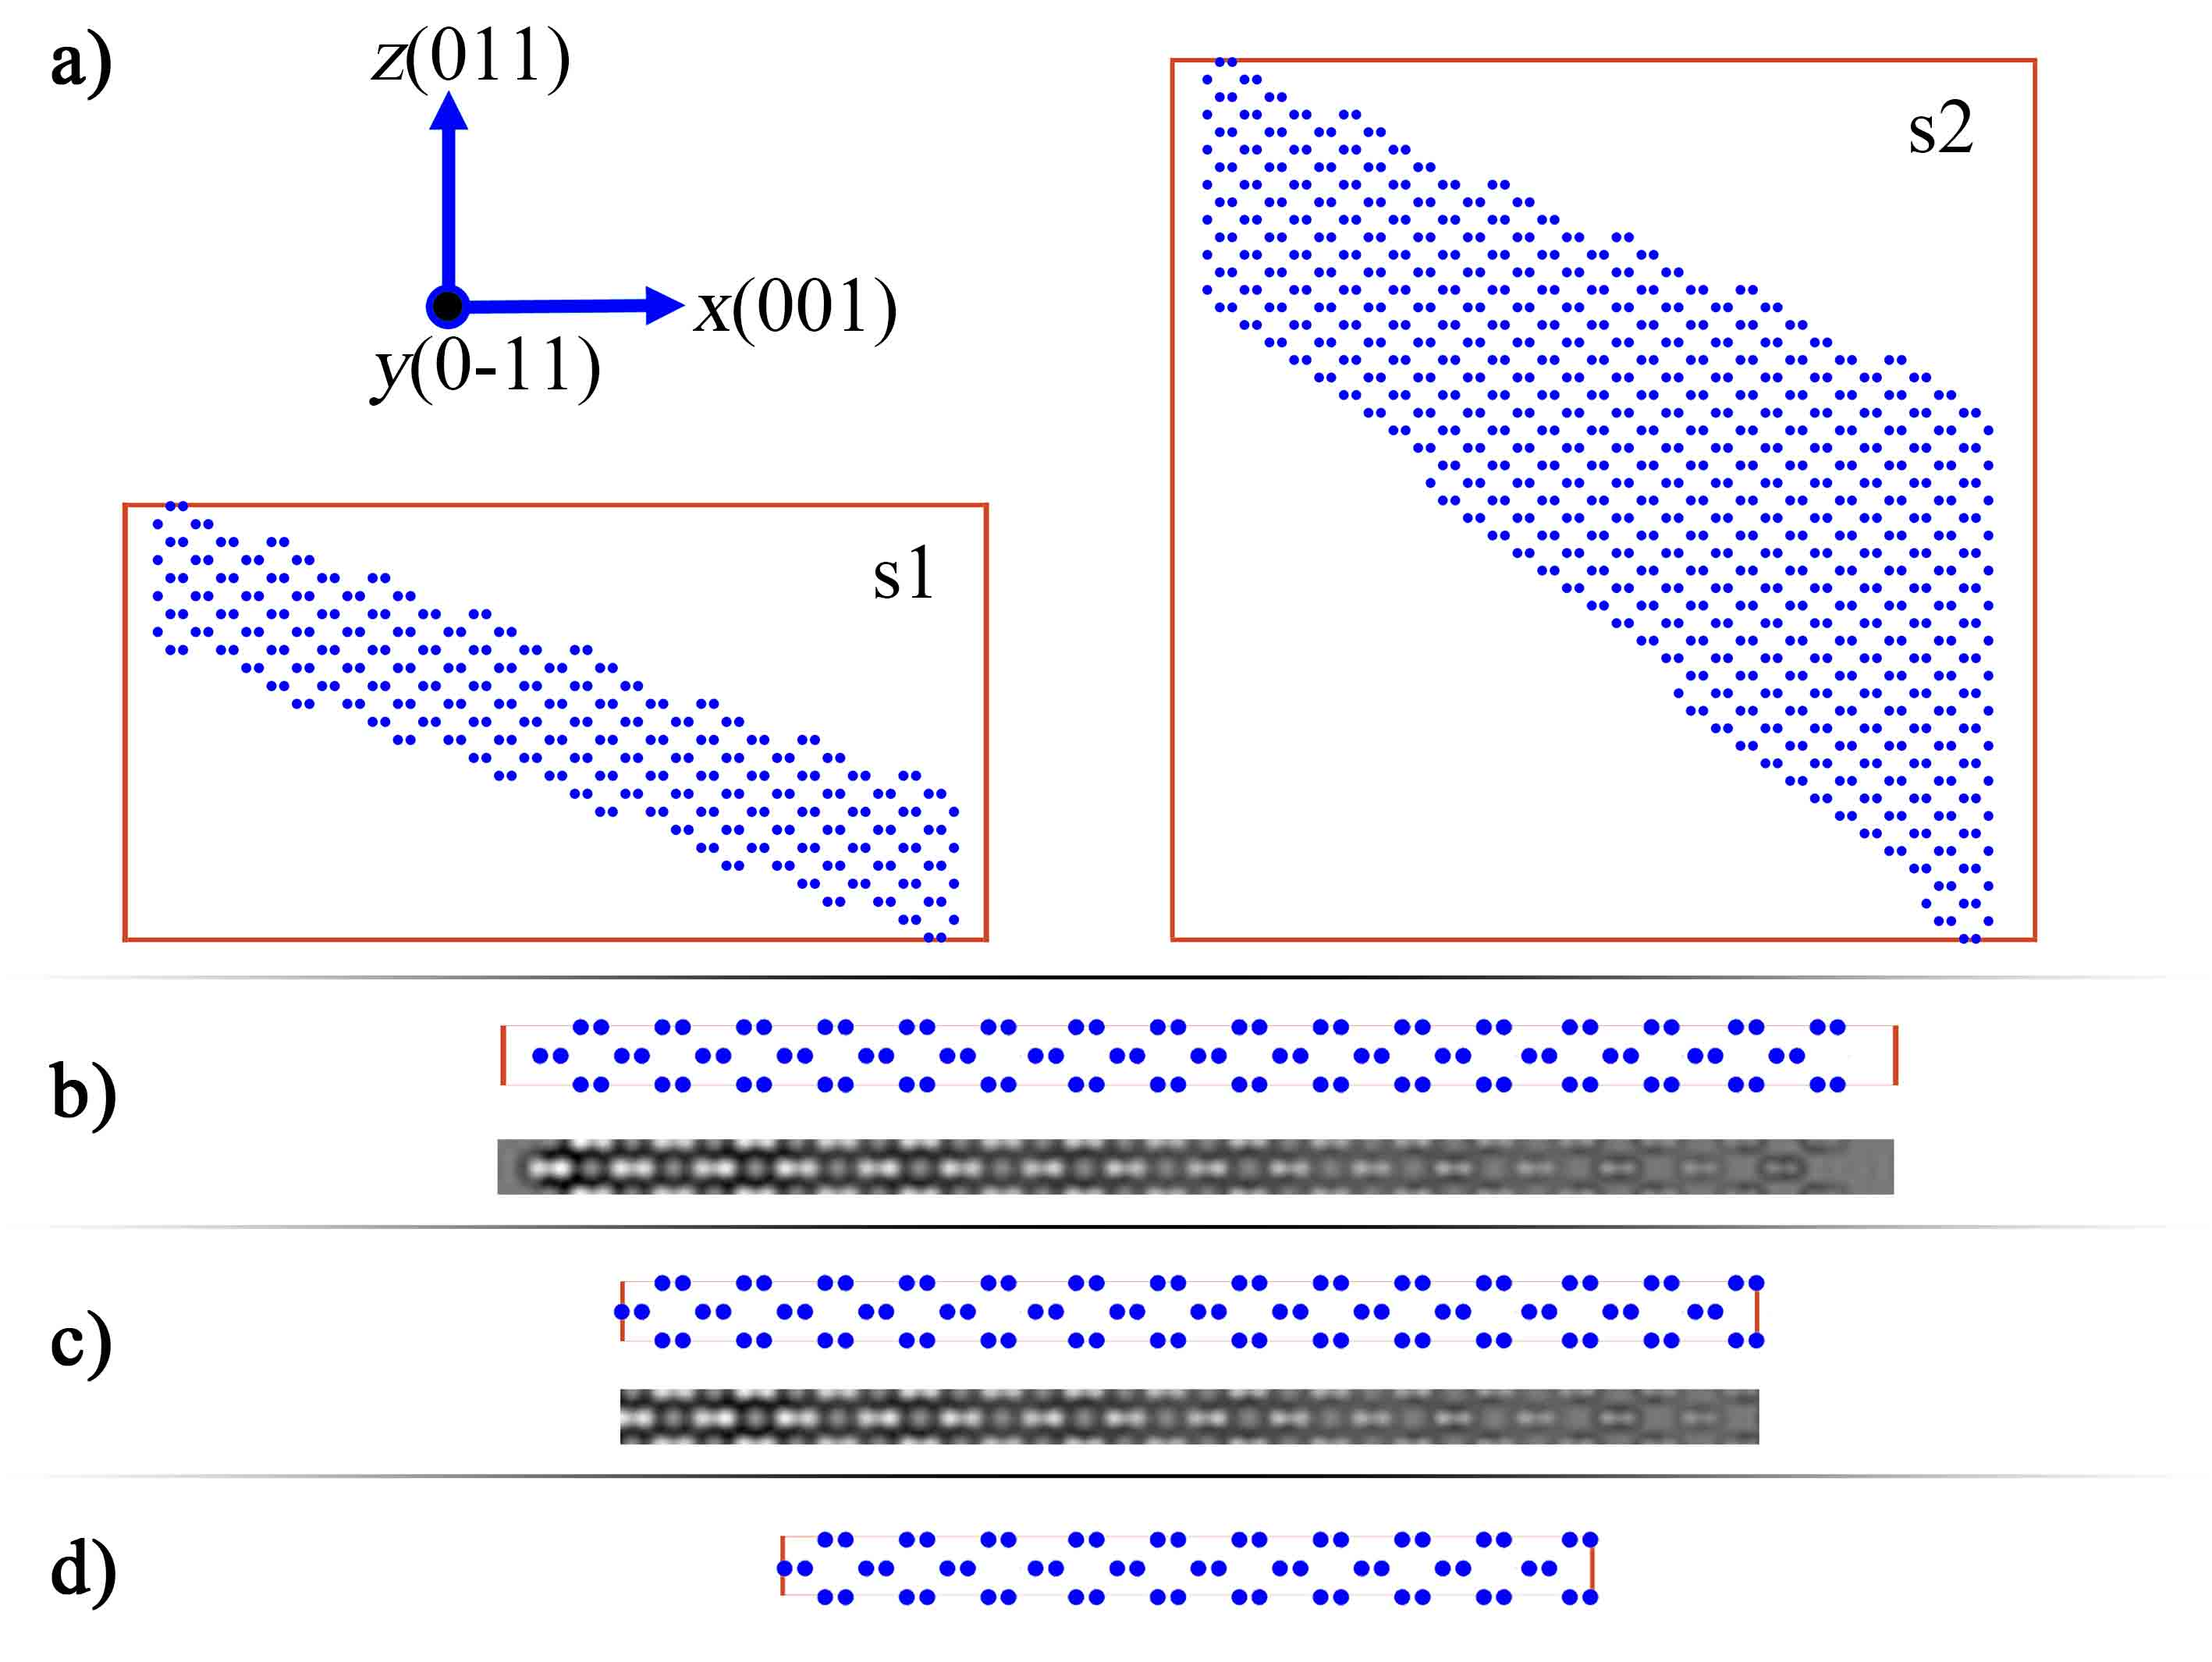
\includegraphics[width=0.9\textwidth]{../2.2/22}
	\caption{超胞 s1 和 s2 的示意图}\label{fig:22}
	\song\tuzhu{a) 超胞 s1 和 s2 的正视图;b) 超胞 s1 和 s2 的俯视图;c) 感兴趣区域的俯视图}
\end{figure}

在模拟测试中,我们讨论了一些重要的参数对全局匹配算法重构的影响,其中包括噪音、欠焦量、晶体倾转、三级球差和 MTF。在实际实验中,这些参数往往无法被精确测定,所以我们还重点探究了这些参数的测量误差对全局匹配算法重构结果的影响。

\begin{table}[htbp]
	\caption{模拟测试中的多层法模拟参数}\label{tab:table1}
	\vspace{0.5em}\centering\wuhao
	\begin{tabular}{cccc}
		\toprule[1.5pt]
		Parameters & Magnitude\\
		\midrule[1pt]
		Side length a & 86.9 $\mathring{A}$ & \\
		Side length b & 3.83 $\mathring{A}$ \\
		\quad\quad\quad\quad\quad Electron beam voltage\qquad\quad\quad\quad\quad & \quad\quad\quad\quad\quad200 kV\qquad\quad\quad\quad\quad \\
		Semi-convergence angle & 0.25 mrad \\
		Objective aperture & 0.7 $\mathring{A}^{-1}$ \\
		Focus spread & 47 $\mathring{A}$ \\
		Debye-Waller factor & 0.5 $\mathring{A}^2$ \\
		Defocus, Cs, crystal tilt, Poisson noise & Zero or specifically defined in tests \\
		\bottomrule[1.5pt]
	\end{tabular}
	\vspace{\baselineskip}
\end{table}

\subsection{模拟测试结果}
\subsubsection{欠焦量、三级球差及晶体倾转对重构的影响}
我们使用全局匹配算法重构了不同欠焦量、三级球差以及晶体倾转下的高分辨 TEM 模拟像以探究这些参数对重构的影响。需要指出的是,在重构中,三级球差和晶体倾转作为已知参数,而欠焦量作为重构的一部分,在重构开始时是未知参数。当 s1 的模拟像中分别加入了 -3 nm 欠焦量、15 $\upmu$m 三级球差或沿 $x-y$ 方向各 15 mrad 晶体倾转后,其重构的结果均如图 4.4a 所示,重构没有误差。同样,当 s2 的模拟像中加入了 -3 nm 欠焦量、15 $\upmu$m 三级球差或沿 $x-y$ 方向 8 mrad 晶体倾转后,其重构结果均如图 4.4b 所示,重构没有误差。然而,当在 s2 的模拟像中加入超过 8 mrad 的晶体倾转时,重构的结果中将产生误差。图 4.4c 是在 s2 的模拟像中加入沿 $x-y$ 方向各 15 mrad 晶体倾转后的重构结果,可见此时重构结果中的误差非常明显。图 4.3d 是在 s2 的模拟像中加入不同程度的晶体倾转产生的误差曲线。可见随着晶体倾转的增加,即使在精确知晓倾转角度时,TEM 像的重构依然将变得越来越困难。

图 4.5a 展示了超胞 s1 和 s2 在欠焦量是 -3 nm 的时候的高分辨 TEM 模拟像。可以看到,图像的衬度随欠焦量的变化发生显著的变化,甚至在某些区域发生了衬度反转的现象(即原子柱的衬度从亮变成了暗)。但即使在这种情况下,全局匹配算法依然可以正确地对其进行重构。图 4.5b 展示了 Si[110] 晶带轴沿 $x$ 方向偏离 8.1 mrad 时的衍射斑点的模拟图像。当晶体倾转为 8.1 mrad 时,电子衍射的偏转已经非常明显。在实际实验操作中,仅通过肉眼观察就能够将晶体倾转控制在 0.4°(约 7 mrad)以内~\cite{Jansen2013}。而且,常规的球差矫正器可以将残余的三级球差控制在 20 $\upmu$m 以内。所以,在球差校正的 TEM 下,经过常规晶带轴校正的 TEM 原子像可以适用于全局匹配算法。以上测试说明了全局匹配算法可以适用于一般的原子分辨率球差矫正 TEM 照片。
\begin{figure}[H]
	\vspace{\baselineskip}
	\centering
	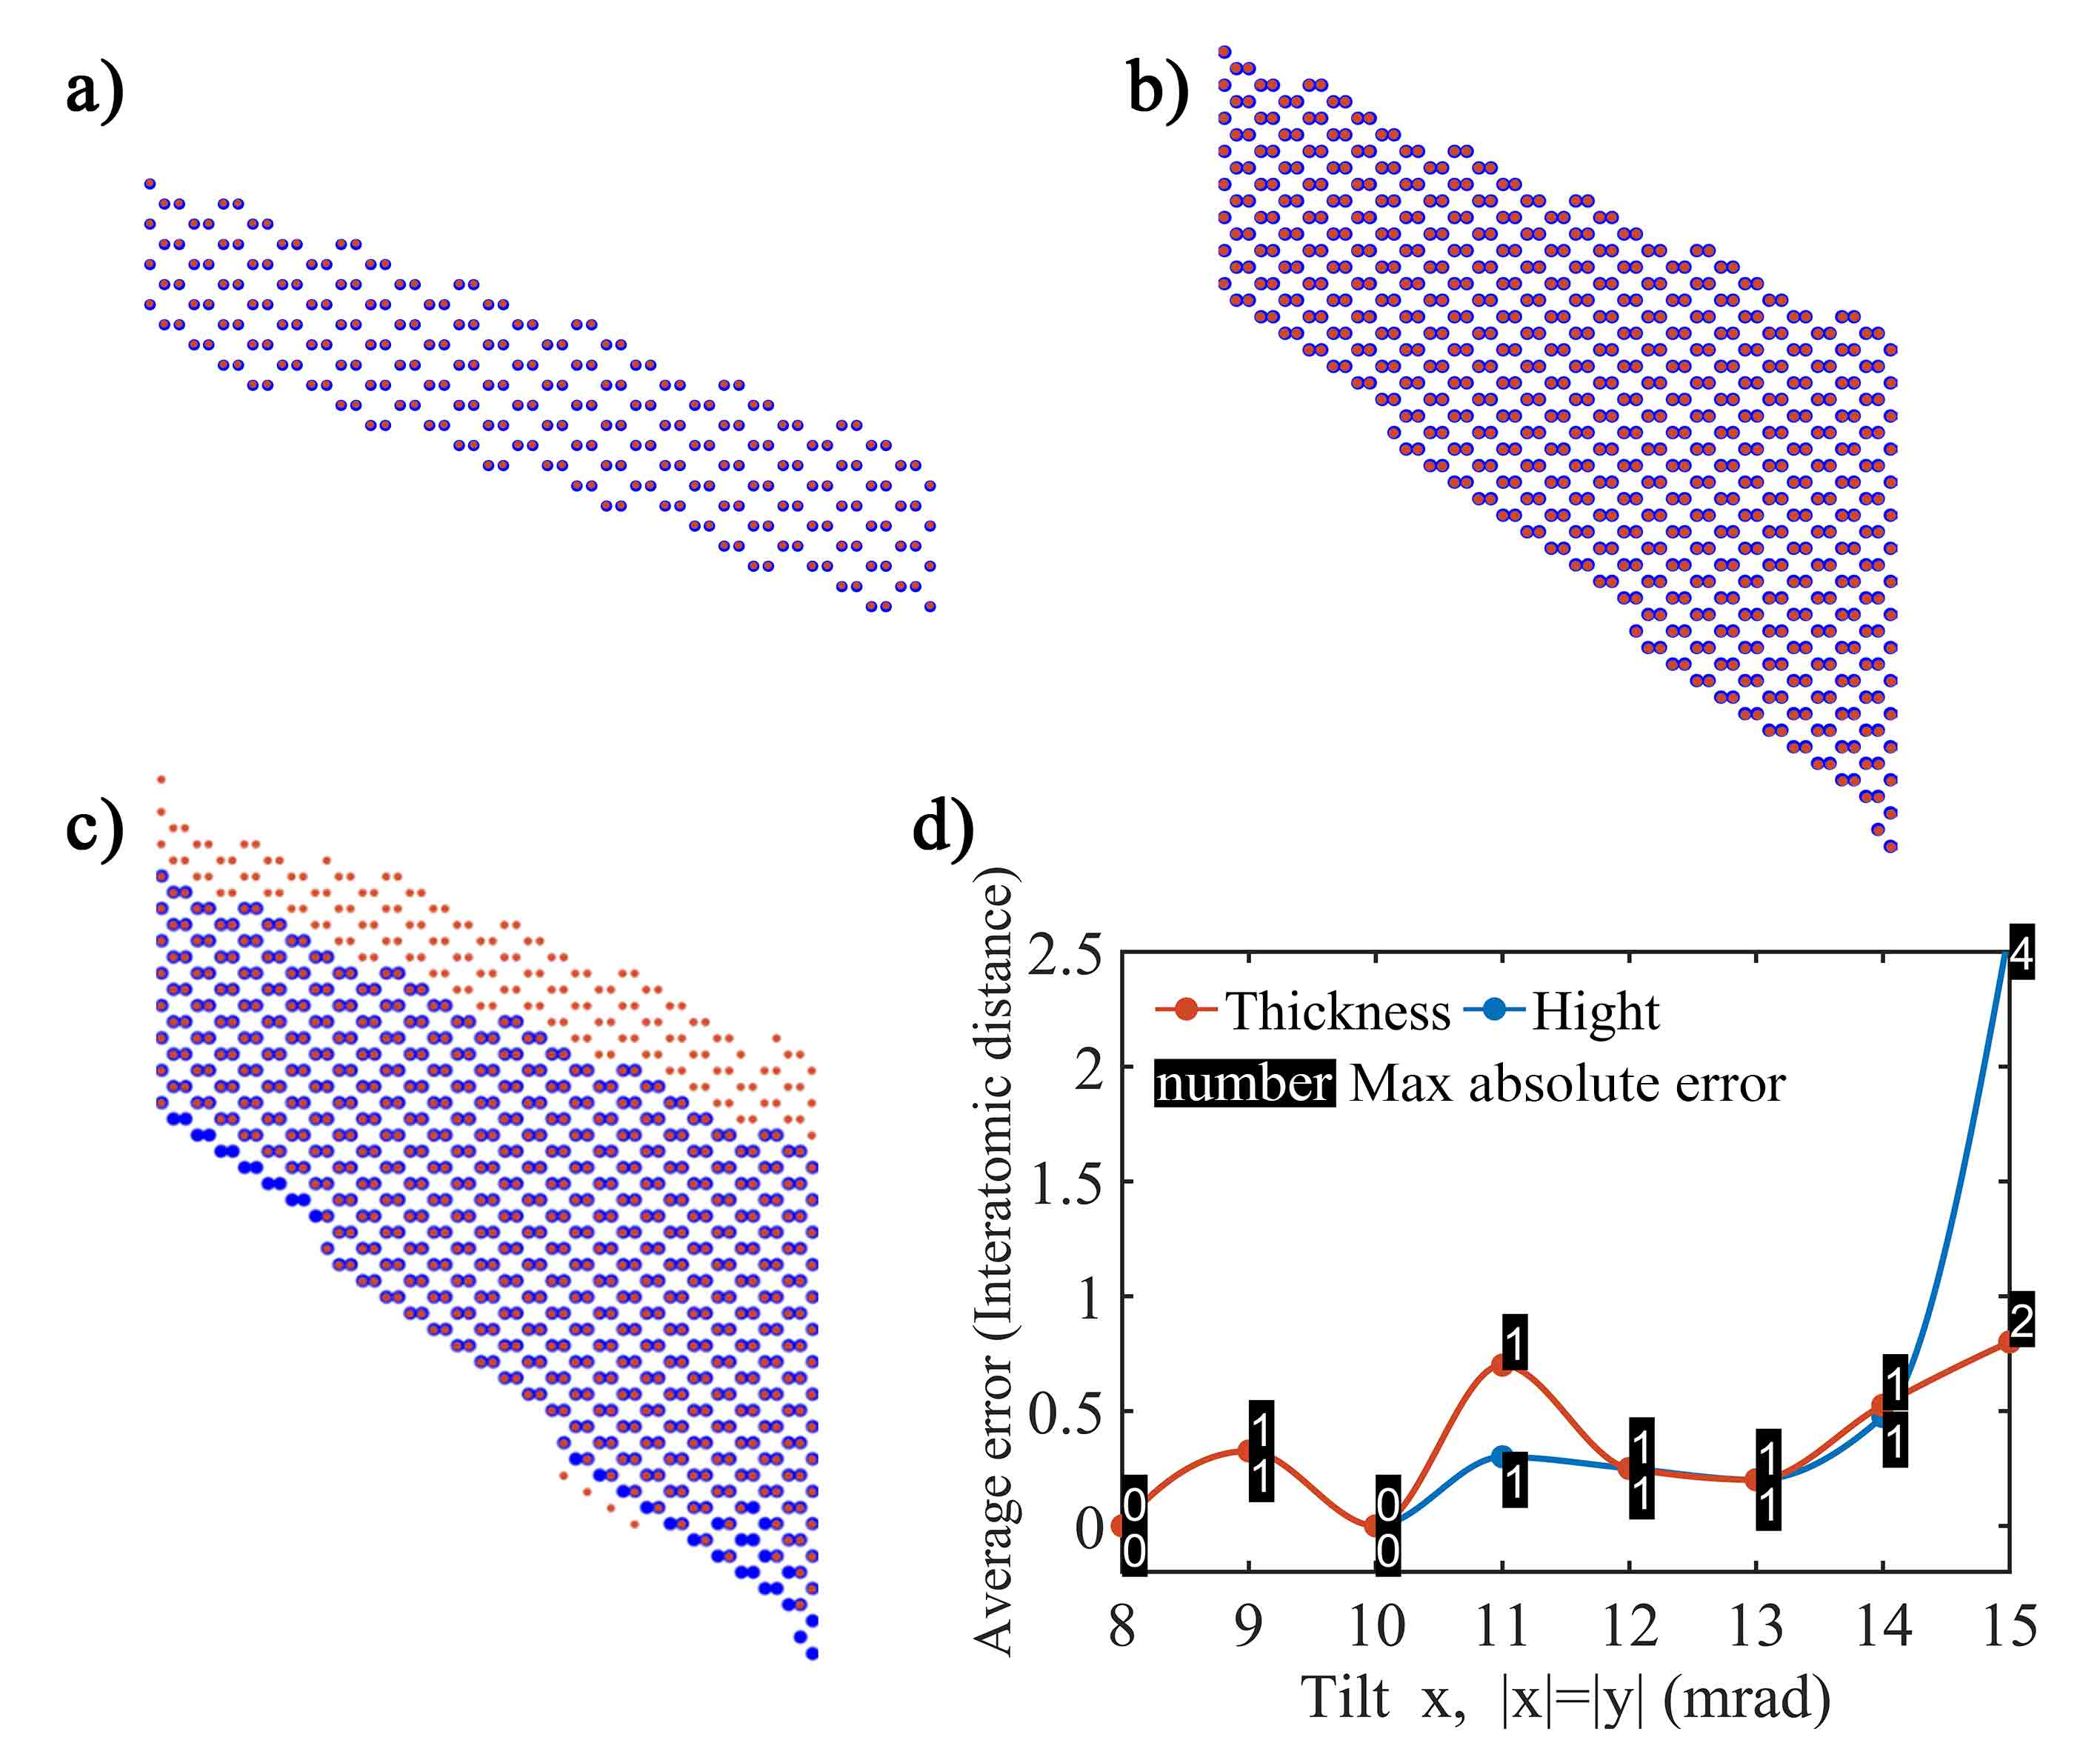
\includegraphics[width=0.75\textwidth]{../2.3/23}
	\caption{模拟测试欠焦量、三级球差、晶体倾转对重构的影响}\label{fig:23}
	\song\tuzhu{a) 当 s1 的模拟像中加入了 -3 nm 欠焦量、15 $\upmu$m 三级球差或沿 $x-y$ 方向各 15 mrad 晶体倾转后的重构结果;b) 当 s2 的模拟像中加入了 -3 nm 欠焦量、15 $\upmu$m 三级球差或沿 $x-y$ 方向各 8 mrad 晶体倾转后的重构结果;c) 当 s2 的模拟像中加入了沿 $x-y$ 方向各 15 mrad 晶体倾转后的重构结果;图 a-c 中背景蓝色原子模型是原始的超胞模型,欠焦红色原子模型是重构结果;d) 当 s2 的模拟像中加入不同程度的晶体倾转后的重构结果的误差变化曲线}
\end{figure}
\begin{figure}[H]
	\vspace{\baselineskip}
	\centering
	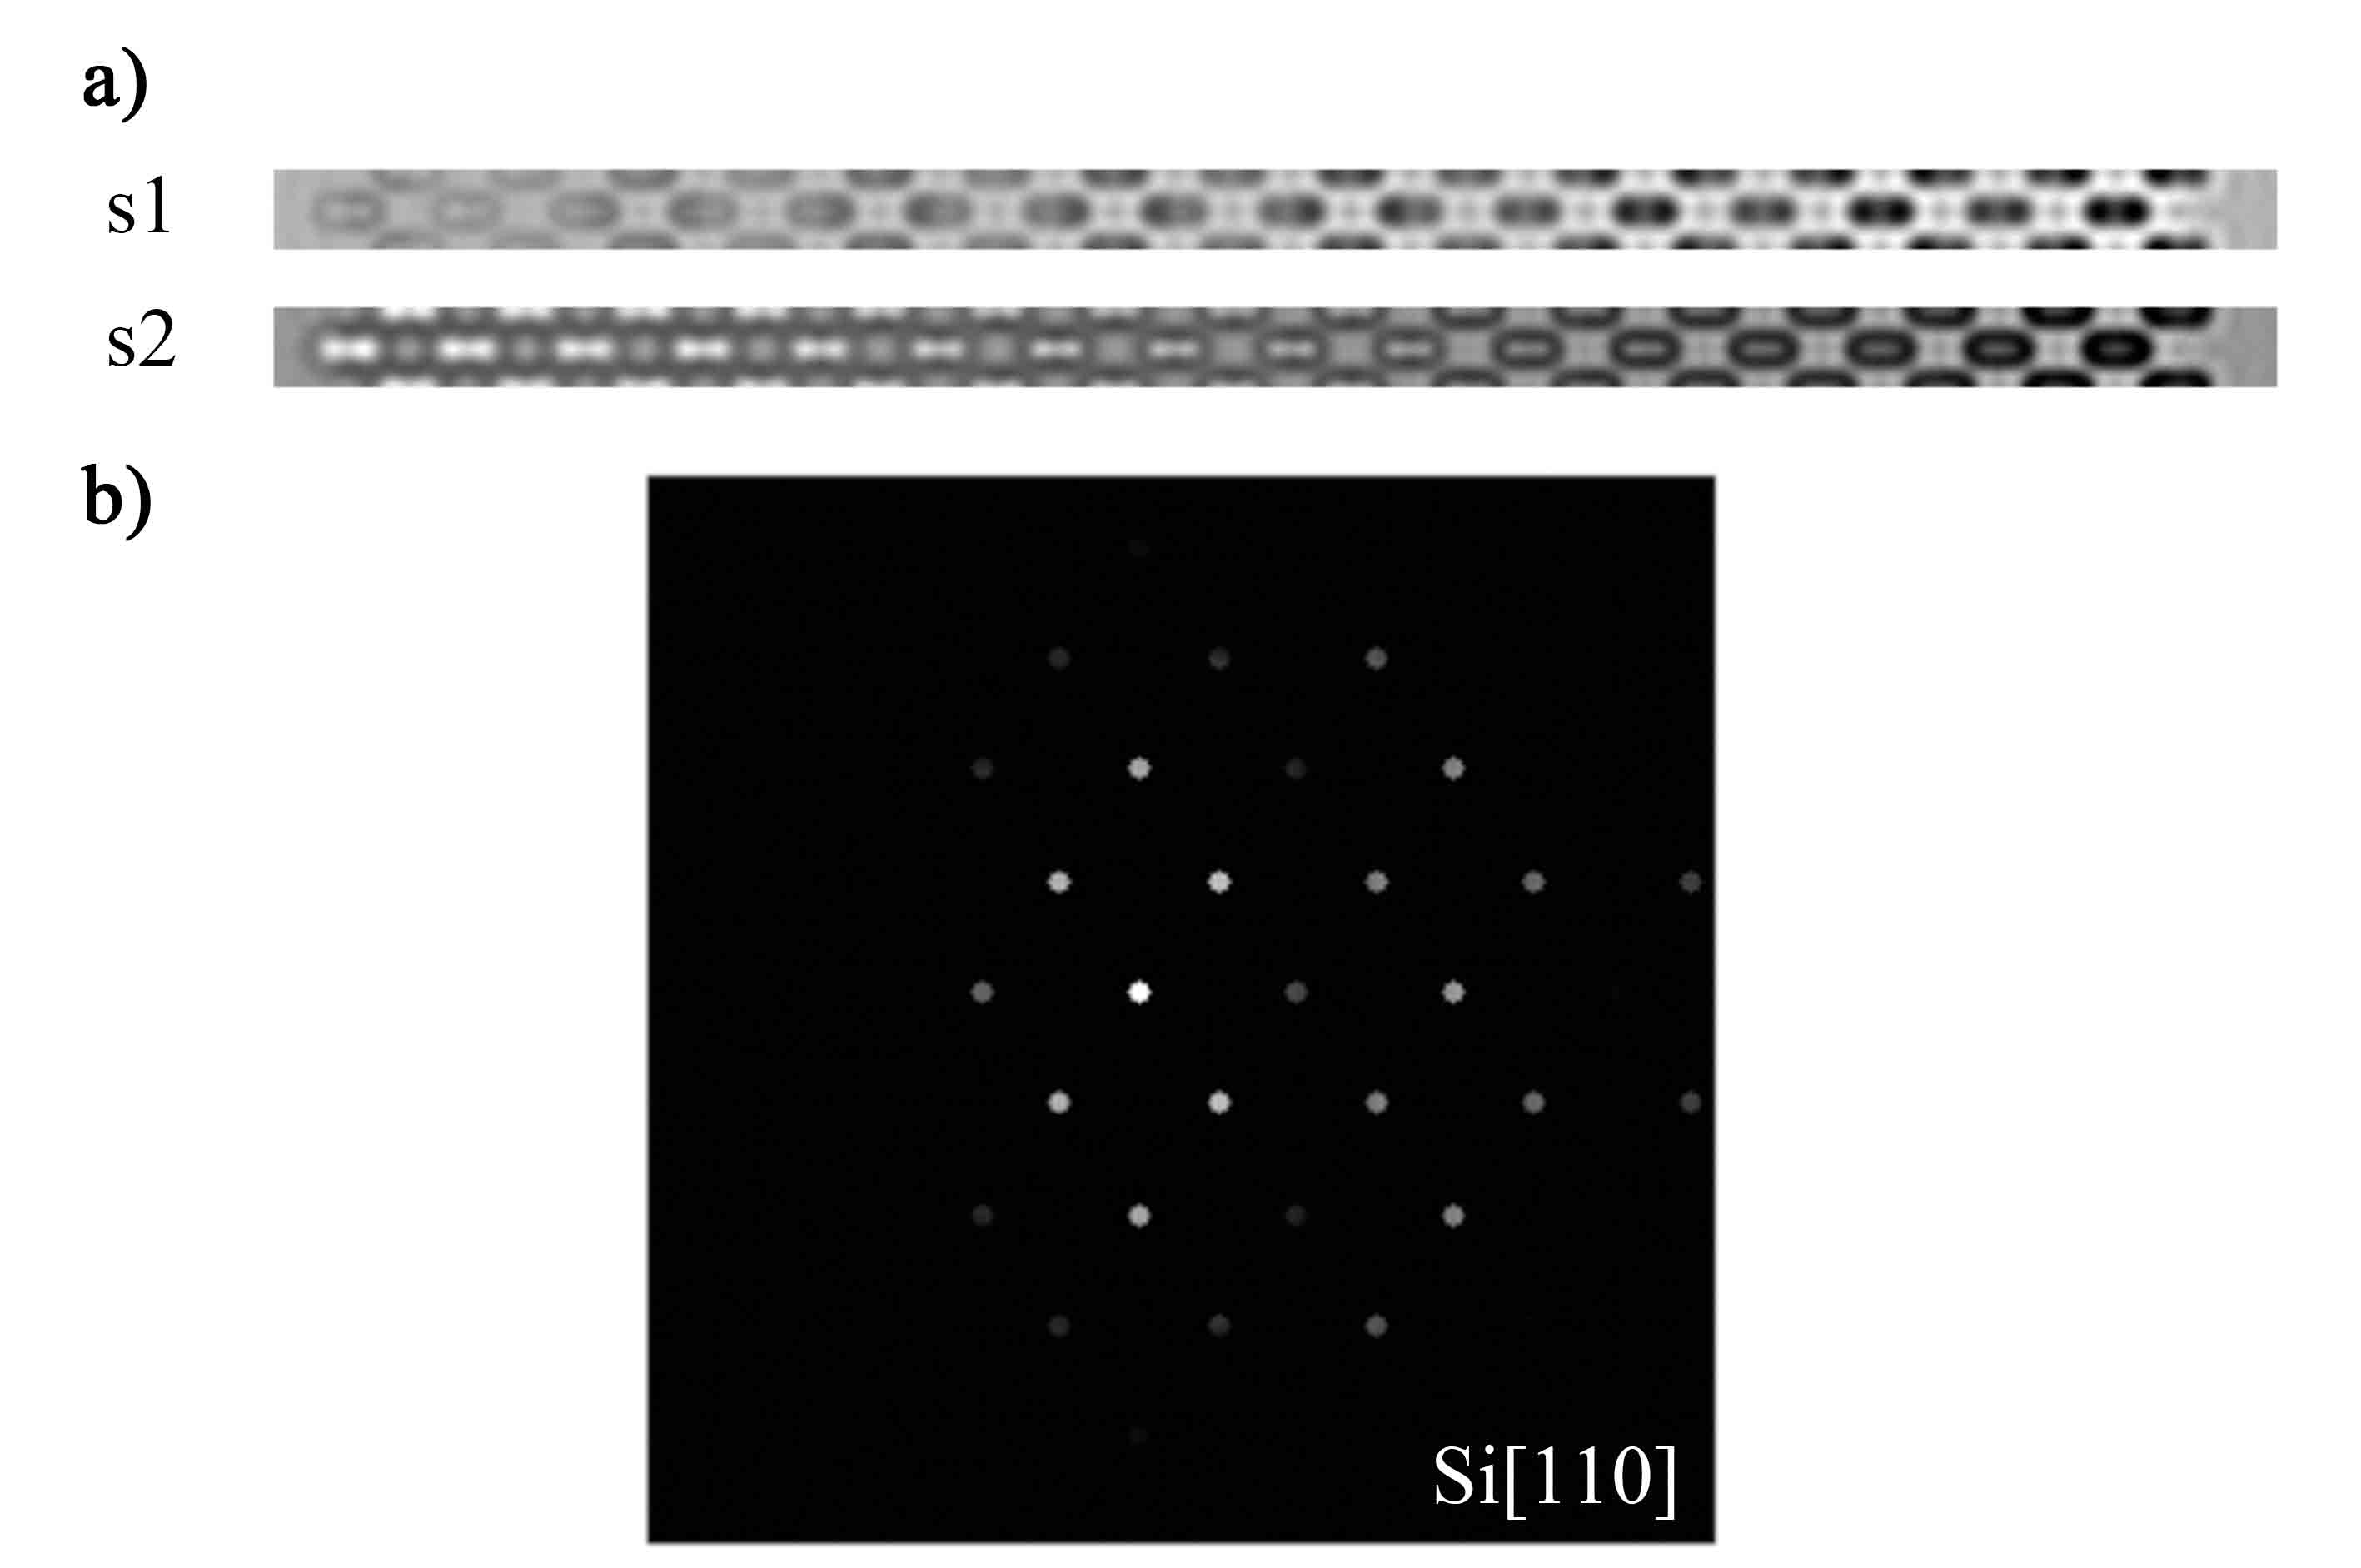
\includegraphics[width=0.75\textwidth]{../2.4/24}
	\caption{超胞 s1 和 s2 在 -3 nm 欠焦量下的模拟像及 Si[110] 在 8.1 mrad 晶体倾转下的电子衍射模拟图}\label{fig:24}
	\song\tuzhu{a) s1 和 s2 在 -3 nm 欠焦量下的模拟像;b) Si[110]晶体在沿 $x$ 方向倾转 8.1 mrad 时的电子衍射模拟图}
\end{figure}

\subsubsection{噪音对重构的影响}

噪音在实验中是不可避免的,它会降低成像质量,影响图像定量分析。为了探究在噪音的存在下,全局匹配算法是否依然能够对图像进行精确重构,我们将泊松噪音加入到了模拟像中,再用全局匹配算法对其进行重构。图 4.6a 和 b 分别展示了当在 s1 和 s2 的模拟像中加入不同信噪比的泊松噪音时的误差变化曲线。可以看到,当信噪比增加到 30 db 时,重构误差几乎消失,当信噪比逐渐降低时,重构误差也将增加。图 4.6c 和 d 展示了加入 30 db 泊松噪音的 s1 和 s2 的部分模拟像。尽管加入的噪音的信噪比相同,但是图 4.6c 和 4.6d 图像质量的下降程度是不同的,这主要是因为 s2 比 s1 厚,所以其 TEM 照片的衬度比 s1 的高,不容易被噪音影响。不过,尽管 s1 的图像质量受噪音的影响如此严重,此时产生的重构误差却很小。所以噪音不会对全局匹配算法产生特别明显的影响。

\begin{figure}[htbp]
	\vspace{\baselineskip}
	\centering
	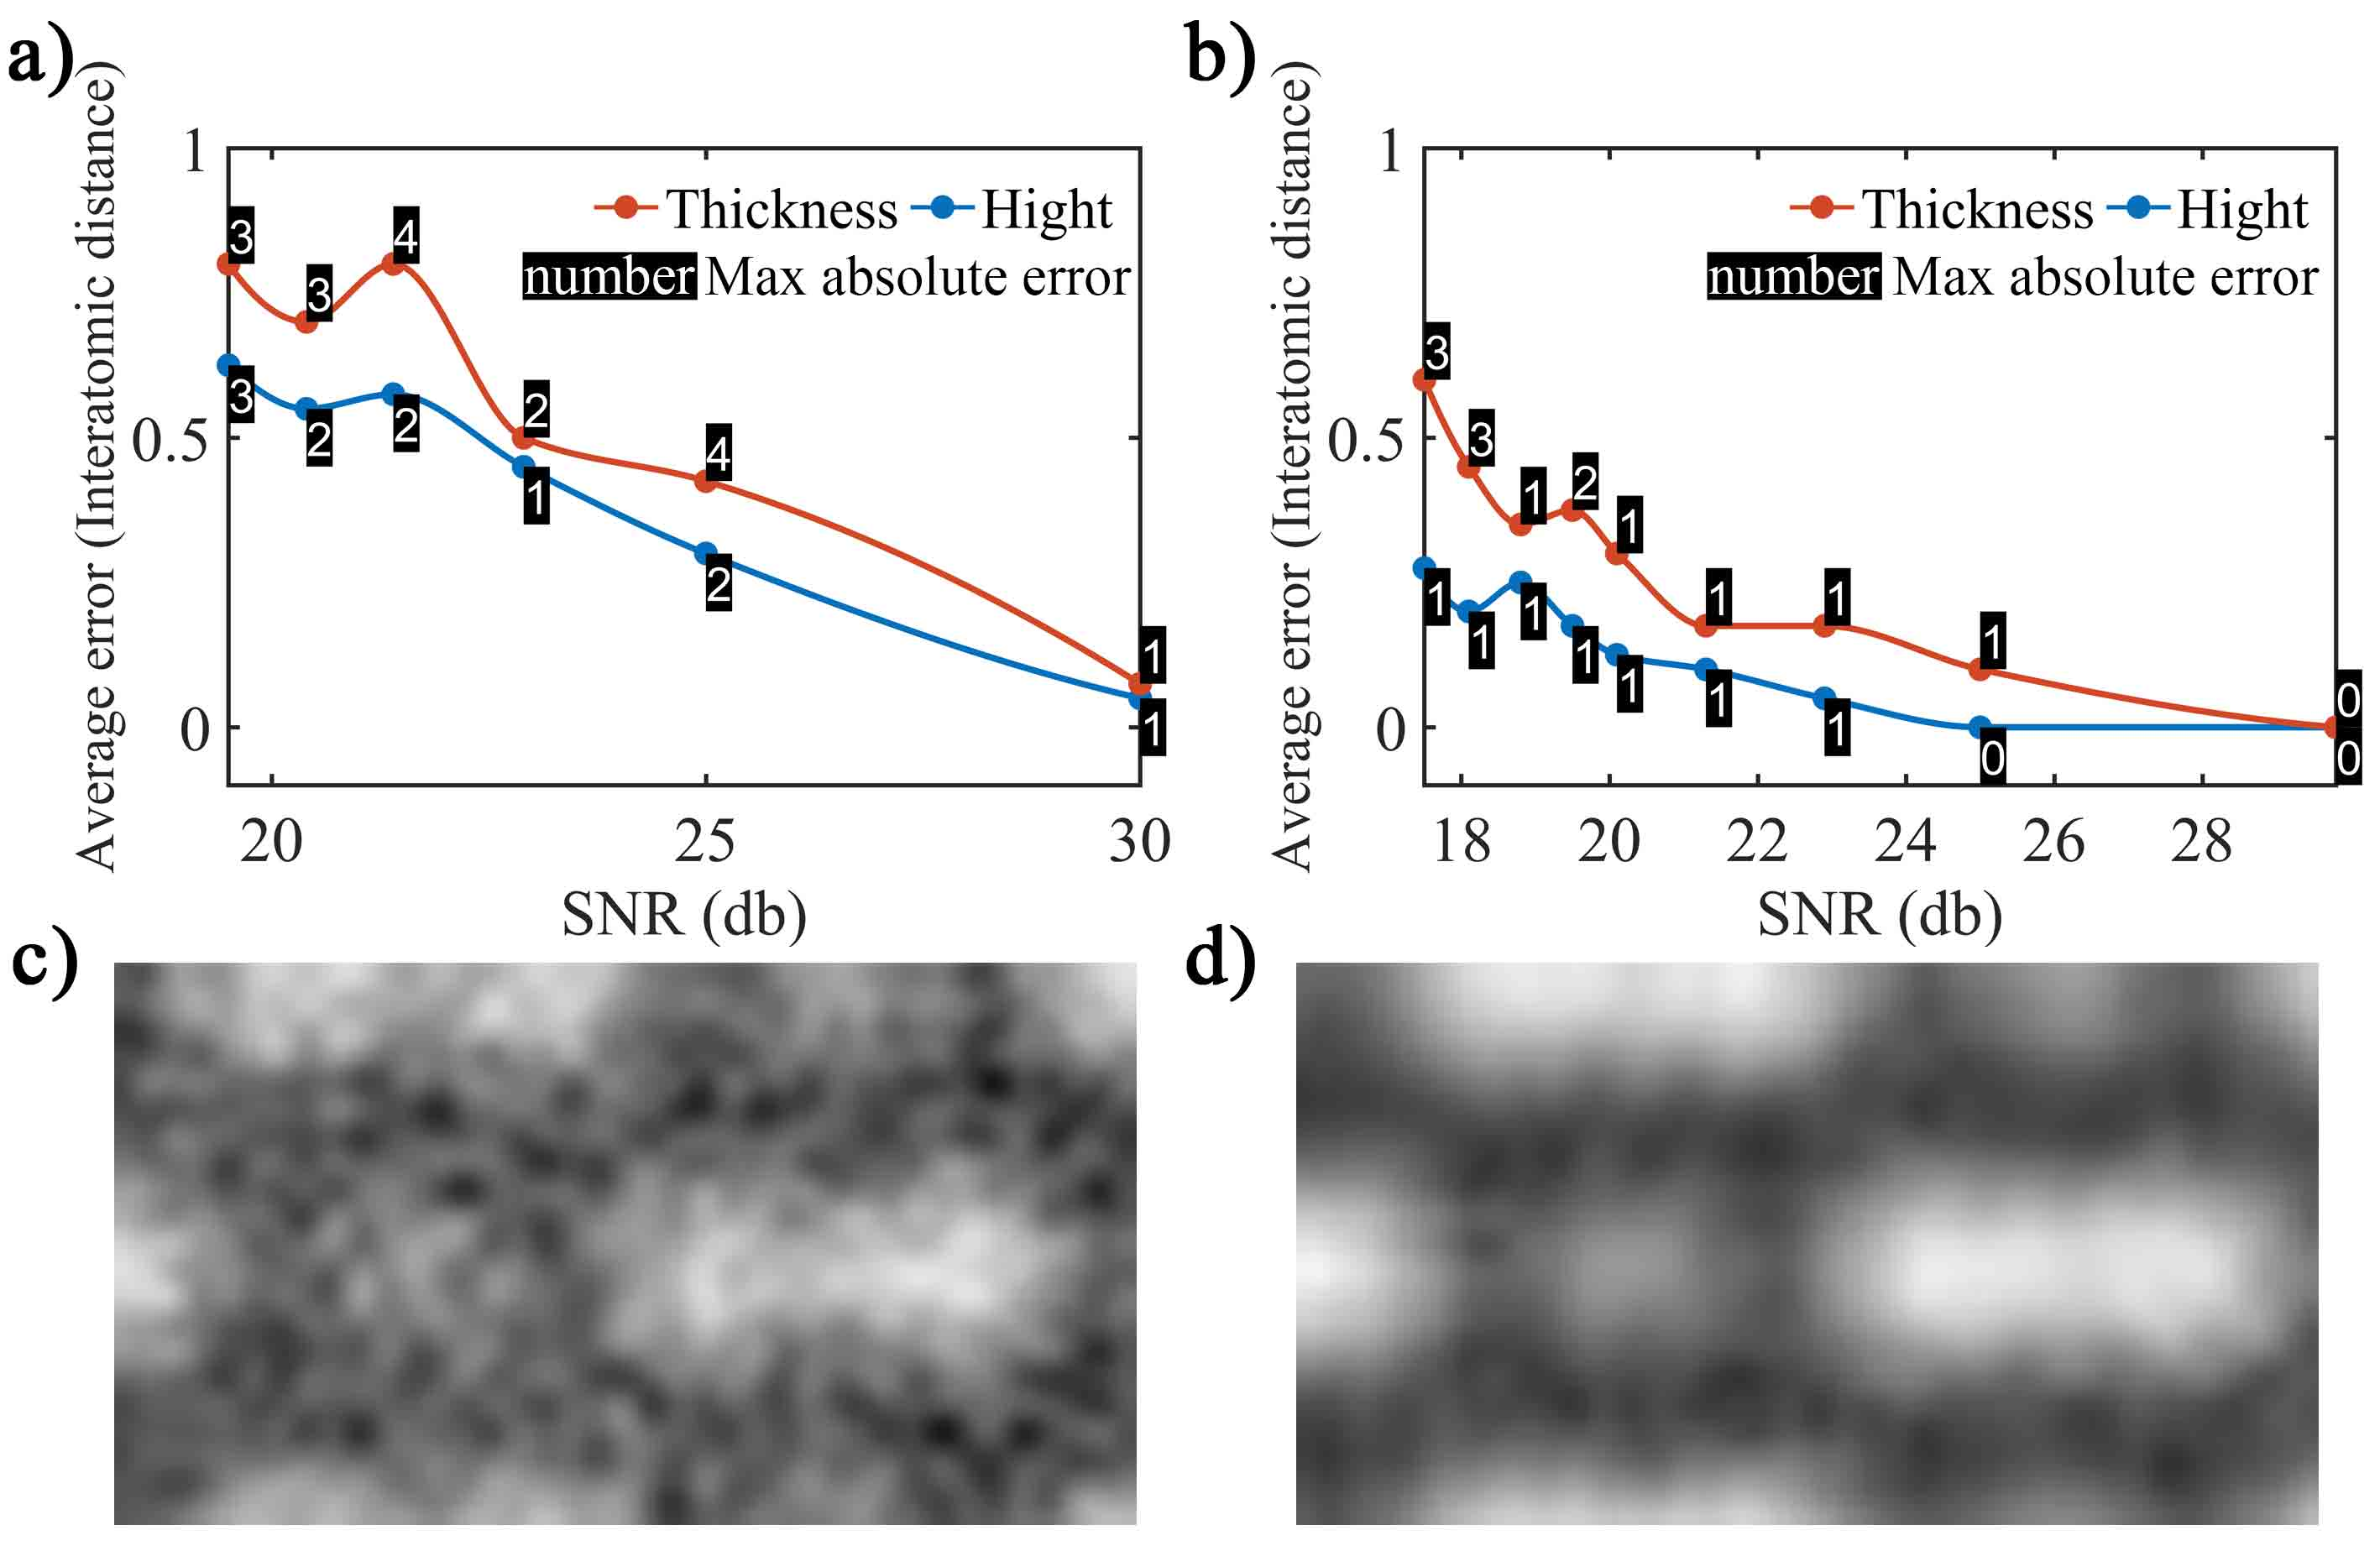
\includegraphics[width=0.9\textwidth]{../2.5/25}
	\caption{模拟测试噪音对重构的影响}\label{fig:25}
	\song\tuzhu{a,b) s1 和 s2 的重构误差关于噪音信噪比的变化曲线;c,d) 加入了 30 db 的泊松噪音后的 s1 和 s2 的部分模拟像}
\end{figure}

\subsubsection{晶体倾转测量误差对重构的影响}
在 TEM 中观察晶体的高分辨图像时,需要倾转晶体使其晶带轴与电子束入射方向平行。在实际操作中,往往无法保证完美地将晶带轴踩正,而残余的晶体倾转又很难被准确地测量。本节通过模拟讨论无法准确知晓晶体倾转的时候是否还能进行精确的三维重构。为此我们首先在 s1 的模拟像中加入了沿 $x$ 和 $y$ 方向各 15 mrad 的晶体倾转,在 s2 的模拟像中加入了沿 $x$ 和 $y$ 方向各 8 mrad 的晶体倾转(在第 4.2.3.1 款 中已经证明,当精确已知晶体倾转时,这两个模型都能被精确重构)。然后,在重构模拟像时使用不同程度的晶体倾转以观察重构结果的变化情况。图 4.7a 和 b 展示了以不同晶体倾转重构 s1 和 s2 时的误差变化曲线。当使用的晶体倾转偏离正确数值时,重构误差逐渐增加。由于 s2 超胞比 s1 厚,所以其高分辨像的衬度变化更易受晶体倾转的影响,在相同的晶体倾转数值偏离下,其产生的重构误差也更大。不过,当晶体倾转的误差保持在几个毫弧度内时,其导致的重构误差在一个单胞长度以内。在 s1 中,晶体倾转的数值偏离引起的重构误差更小,在一定程度内几乎可以被忽略。所以,晶体倾转的测量误差对厚样品的重构具有一定的影响。不过,厚样品的图像衬度受晶体倾转的影响较大,在实际使用时只要保证使用高质量的 TEM 像就可以避免过大的晶体倾转带来的误差。
\begin{figure}[htbp]
	\vspace{\baselineskip}
	\centering
	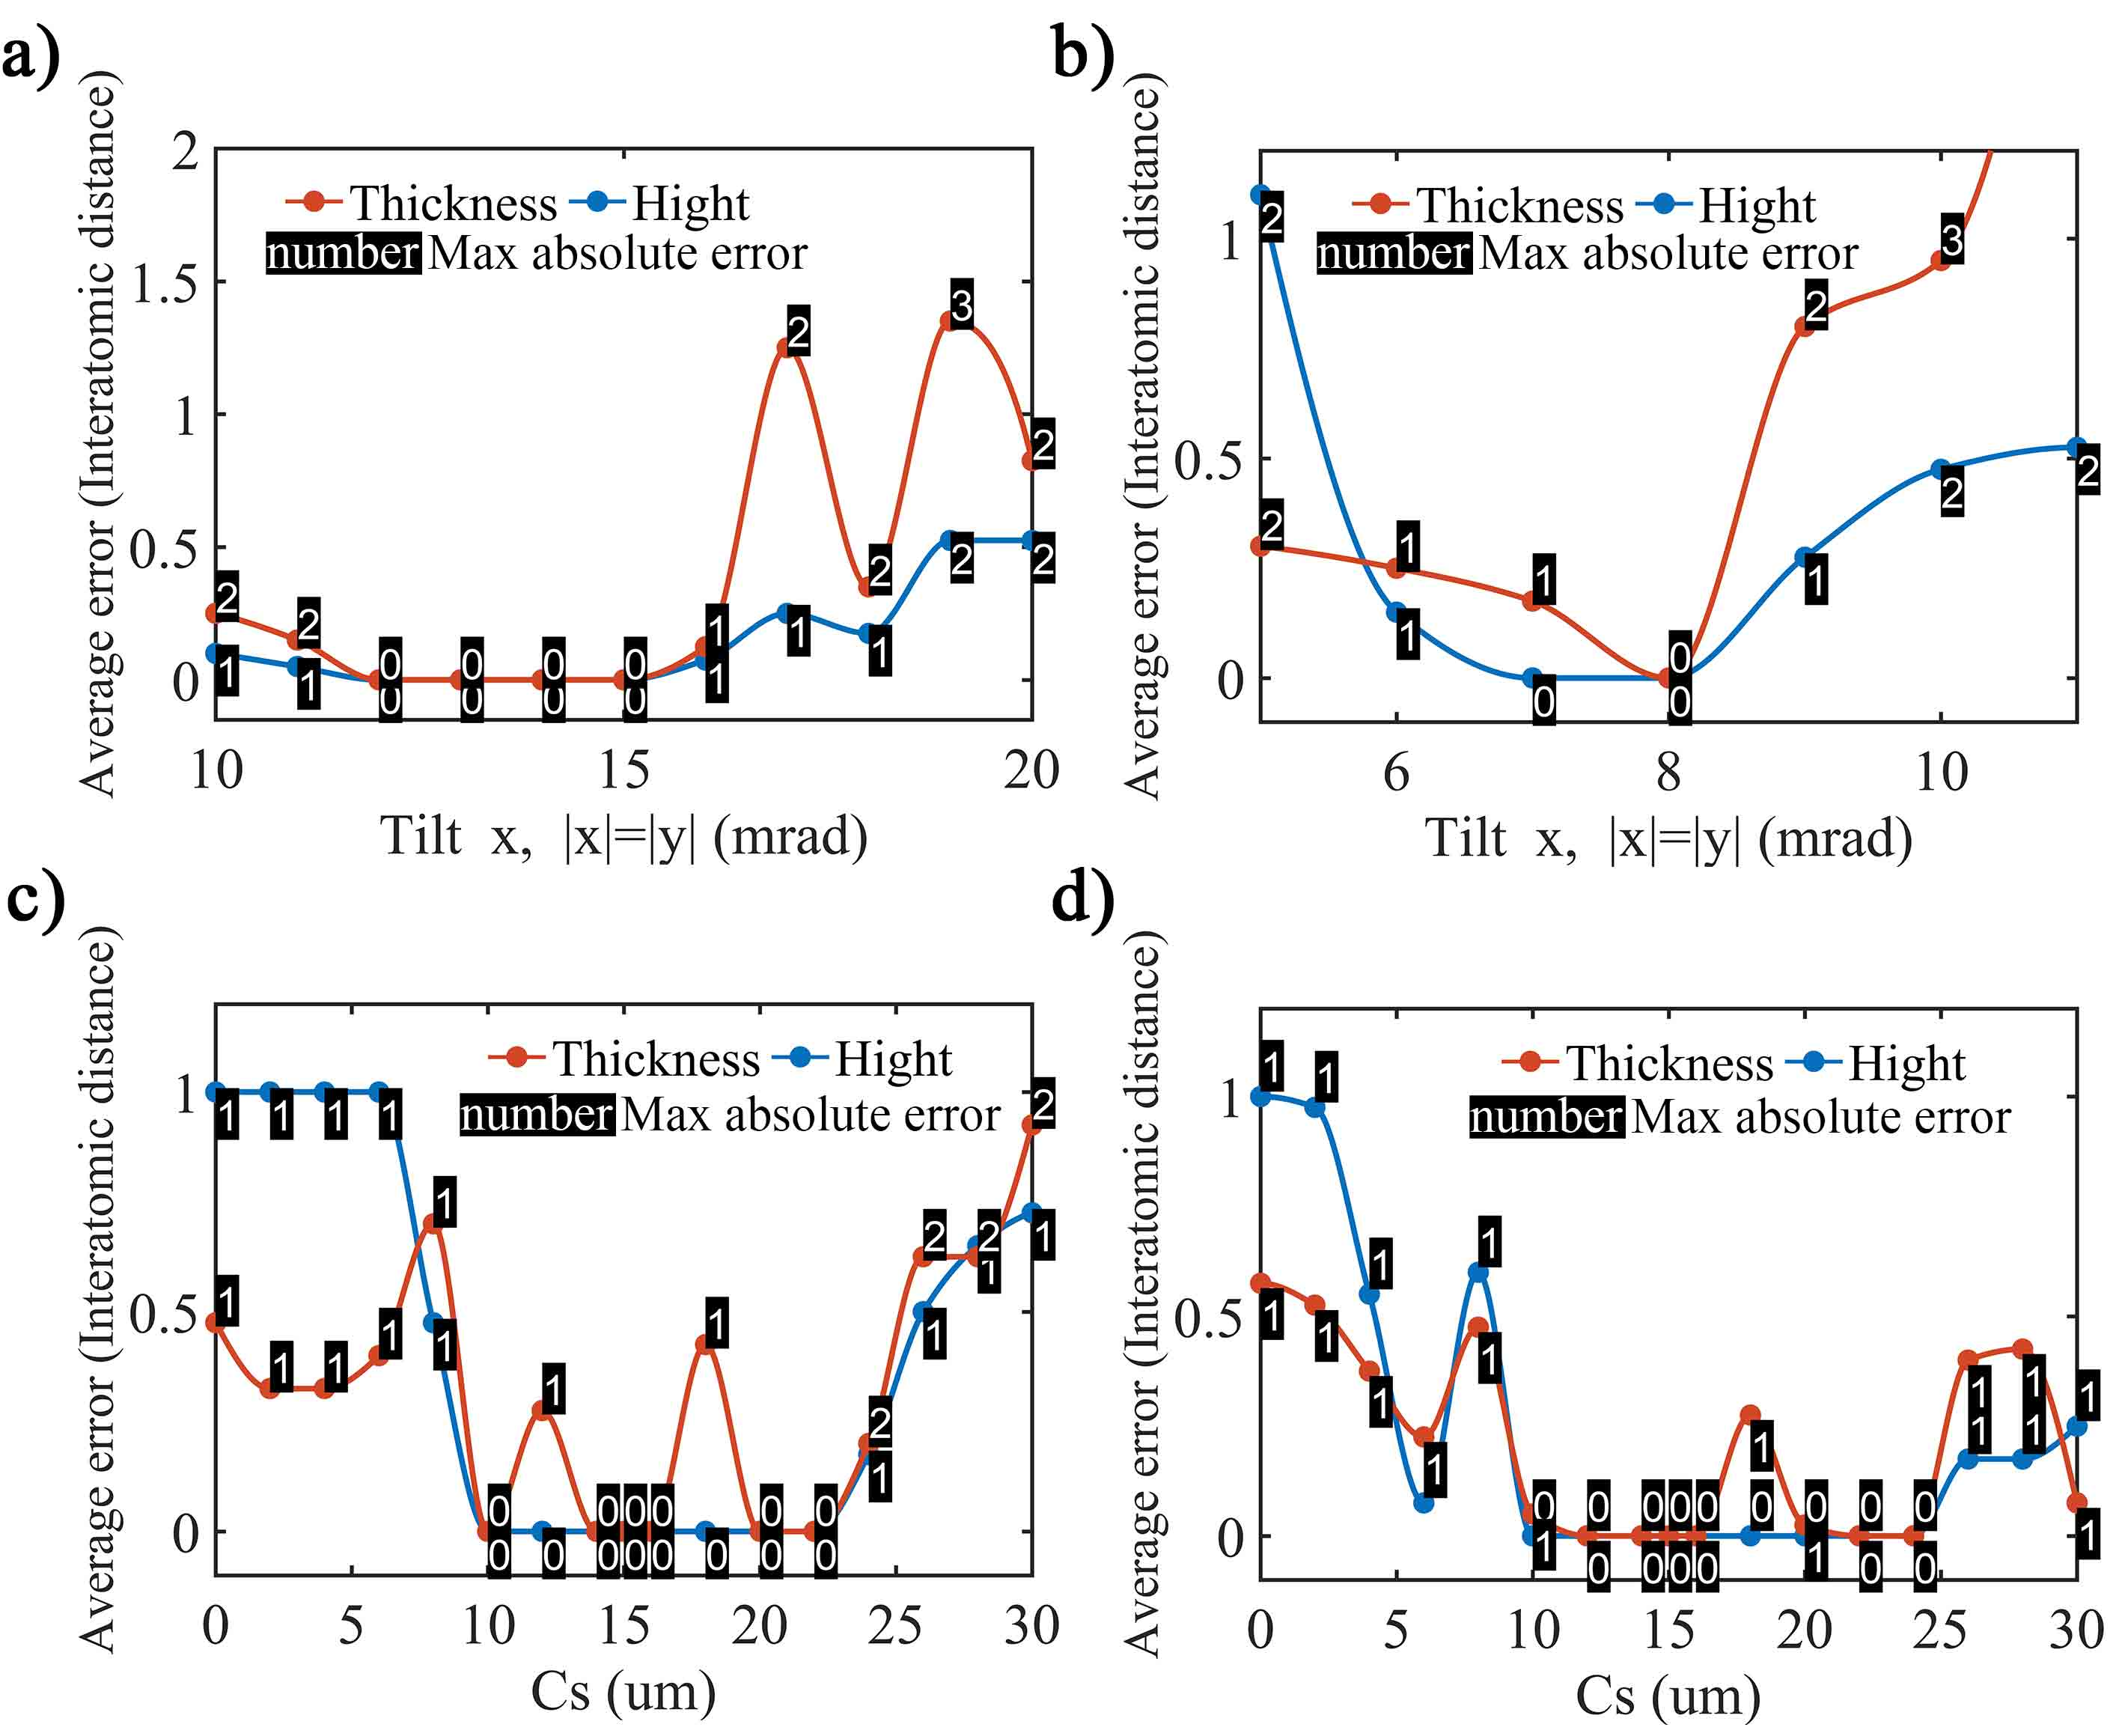
\includegraphics[width=0.9\textwidth]{../2.6/26}
	\caption{模拟测试晶体倾转以及三级球差测量误差对重构的影响}\label{fig:26}
	\song\tuzhu{a) 以不同程度的晶体倾转重构含 15 mrad 晶体倾转的 s1 模拟像时的误差变化曲线;b) 以不同程度的晶体倾转重构含 8 mrad 晶体倾转的 s2 模拟像时的误差变化曲线;c) 以不同程度的三级球差重构含 15 $\upmu$m 三级球差的 s1 模拟像时的误差变化曲线;d) 以不同程度的三级球差重构含 15 $\upmu$m 三级球差的 s2 模拟像时的误差变化曲线}
\end{figure}

\subsubsection{三级球差测量误差对重构的影响}
三级球差(third order spherical aberration,Cs)是 TEM 成像过程中非常重要的像差参数,在球差矫正器发明之前,它一直是限制 TEM 分辨率的重要因素。在实际的实验中,尽管球差矫正器能够将三级球差矫正到很小量级,但是其测量到的球差与真实的球差之间总可能存在误差。当无法准确知道真实球差的数值时,是否还能进行精确的三维重构是一个需要被探究的问题。本节在 s1 和 s2 的模拟像中都加入了 15 $\upmu$m 的三级球差,并在重构时,使用不同数值的三级球差。图 4.7c 和 d 是以不同的三级球差重构 s1 和 s2 时的重构误差变化曲线。当三级球差的测量误差在 $\pm$5 $\upmu$m 以内,重构的平均误差将保持在 0.4 个单胞长度以内,且最大误差不超过 1 个单胞长度,这说明重构的结果中只有少数原子柱产生一个单胞长度的重构误差。总体而言,三级球差对重构结果的影响不大,即使存在一定的常规测量误差,也可以进行准确的三维重构。

\subsubsection{MTF 矫正误差对重构的影响}

在电镜中,CCD 相机收集到的图像强度与理论上的图像强度是不一致的,MTF 函数描述了两者之间的关系。公式(4.4)是公式(1.23)简化 $MTF_{px}$ 和 $C$ 之后的结果:
\begin{equation}
H=F \cdot \textit{MTF}_{px}
\end{equation}
其中 $H$ 表示 $CCD$ 相机收集到的 TEM 照片的傅里叶变换,$F$ 表示理想的 TEM 照片的傅里叶变换,$\textit{MTF}_{px}$ 如下式所示~\cite{VanBroek2012}:
\begin{equation}
\textit{MTF}_{px}(u,v)=\exp\left(-\alpha \sqrt{u^2+v^2}\right)
\end{equation}
$\alpha$ 是可变的参数,$u$ 和 $v$ 表示倒空间坐标。



在定量分析电镜照片之前,通常需要先测量 CCD 相机的 MTF 曲线,消除 MTF 对图像衬度的调制。本节讨论了当测量得到的 MTF 与实际的 MTF 有偏差时三维重构的结果的变化情况。首先使用 $\alpha = 5$ 时的 MTF 函数对在 s1 和 s2 的模拟像进行调制,然后分别使用不同 $\alpha$ 对应的 MTF 函数来矫正模拟像,再用全局匹配算法重构这些矫正之后的图像。图 4.8a 展示了这些图像的衬度变化曲线。其中,s1 的无 MTF 调制的模拟像的衬度(使用 
$\alpha = 5$ 的 MTF 函数矫正后的图像) $CON_{s1}$ 是 0.052,当使用 $\alpha = 4.5\sim5.5$ 对应的 MTF 函数矫正后,这些图像的衬度是 $0.041\sim0.062$,相当于 $CON_{s1} / 1.27\sim CON_{s1} \times 1.27$。相应的,s2 的无 MTF 调制的模拟像的衬度 $CON_{s2}$ 是 0.246,矫正后的图像衬度是 $0.195\sim0.316$,也相当于 $CON_{s2} / 1.27\sim CON_{s2} \times 1.27$。可见 s1 和 s2 对应的图像的衬度变化幅度是相同的。$\textnormal{图 4.7b 和 c}$ 展示了重构这些矫正后的图像时的误差变化曲线。当 $\alpha$ 偏离正确数值“5”时,对应的重构误差也会增大。而且,s2 中产生的重构误差明显高于 s1 中的误差,这是因为 s2 的模拟像本身的衬度较高的原因。图 4.8d 展示了 s1 中每一个原子柱处产生的厚度误差。当使用 $\alpha
 < 5$ 对应的 MTF 矫正图像后,这些图像的重构结果的每个原子柱都比原始(s1) 的原子柱厚;相反,当使用 $\alpha > 5$ 时对应的 MTF 矫正图像后,这些图像的重构结果比原始结构薄。这说明 MTF 的矫正误差,会有规律地影响重构结果的厚度。综上可知,MTF 对重构的影响较为严重,在定量分析和重构时是不可忽略的因素,需要被精确地测量。
 
 \begin{figure}[H]
 	\vspace{\baselineskip}
 	\centering
 	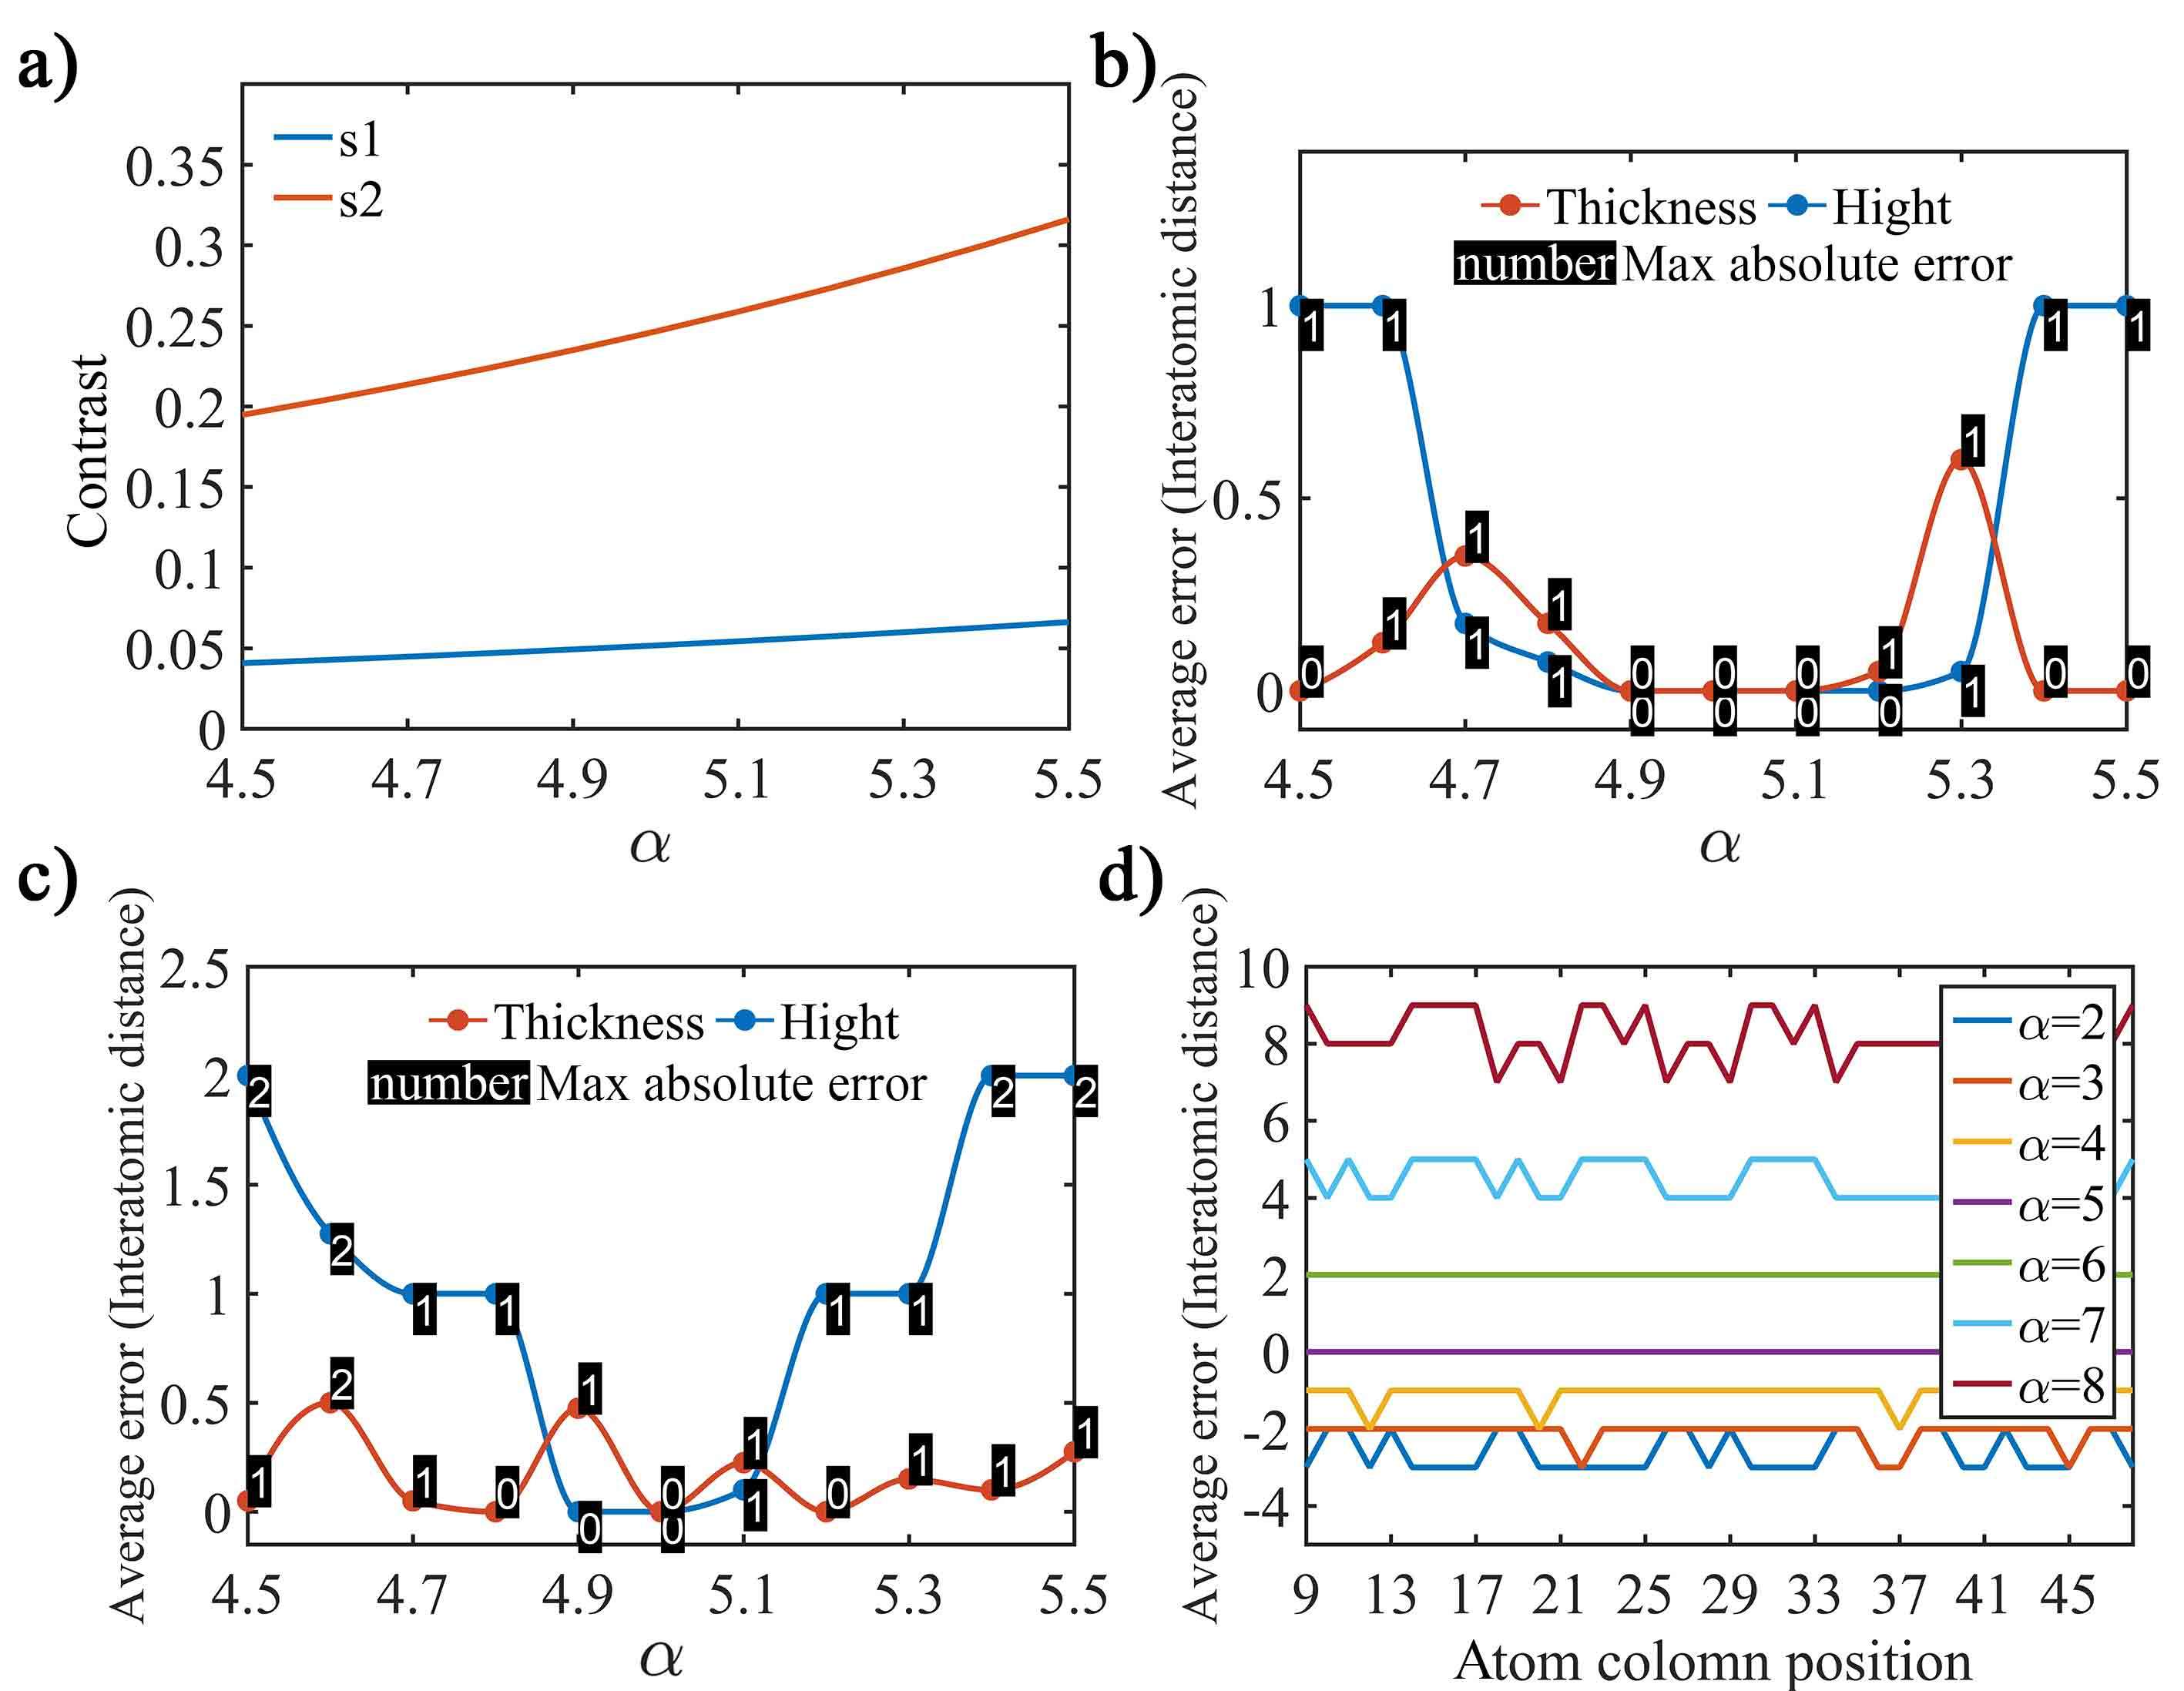
\includegraphics[width=0.8\textwidth]{../2.7/27}
 	\caption{模拟测试 MTF 对重构的影响}\label{fig:27}
 	\song\tuzhu{a) 不同 $\alpha$ 对应的 MTF 矫正 s1 和 s2 的模拟像后图像衬度的变化曲线,其中 s1 和 s2 的模拟像均加入了 $\alpha = 5$ 对应的 MTF 曲线的影响;b,c) 不同 $\alpha$ 对应的 MTF 矫正 s1 和 s2 的模拟像后的图像的重构误差曲线;d) 不同 $\alpha$ 对应的 MTF 矫正 s1 的模拟像后的图像经重构后,所有原子柱的厚度误差}
 \end{figure}
 \subsubsection{模拟测试小结}
 本节提出了从单张原子分辨 TEM 照片重构晶体材料的三维形貌的全局匹配算法。模拟测试证明了全局匹配算法比局部匹配算法的重构结果更加准确。我们还在模拟测试中分析讨论了多个因素对重构结果的影响,结果显示全局匹配算法可以适用于一般的球差矫正 TEM 拍摄得到的原子分辨率 TEM 照片。具体地,当晶体的晶带轴被校正的情况下,即使其中存在残余晶体倾转,全局匹配算法的重构精度也不会受太大影响。另外,欠焦量、三级球差、噪音等对重构精度的影响更加微弱。不过,MTF 对重构结果的影响特别明显,其在图像定量分析中是不可忽视的因素,在重构之前需要被准确地测量。

\section{三维重构方案的自洽性}
\subsection{环绕效应收敛测试}
在第 1.2.4.3 款已述及,环绕效应会导致图像模拟误差。在多层法运算过程中,每一层运算都会有误差被包裹到图像中。而这种产生于边界的误差,能够向图像内部扩散至多深,是相当复杂的一个问题,取决于样品厚度、成像条件等诸多因素。因此,为了保证全局匹配算法中图像模拟的精确性,必须避免这种由图像计算时的周期性假设所导致的误差。这意味着,在模拟感兴趣区域的高分辨 TEM 照片时使用的超胞模型必须大于感兴趣区域,以阻挡环绕效应影响到感兴趣区域的图像衬度。而在图像匹配时,只使用感兴趣区域的图像与实验图像对比。如图 4.9 所示,为了确定超胞模型的必要尺寸,我们对不同大小的模型进行了收敛测试。

在收敛测试中,如图 4.9a 所示,我们将感兴趣区域的超胞标记为 \textbf{0},将一系列不同尺寸的超胞标记为 \textbf{0},\textbf{1},…,\textbf{6}。接着,计算出这些超胞的模拟像 $I_i(x, y)(i = 0,\cdots, n)$,这些图像的尺寸当然也各不相同。对于连续的两张图像,我们在图像 $I_0$ 对应的区域计算出它们的差 $\Delta I_i(x, y) = I_{i+1}(x, y)$ – $I_i(x, y)$,如图 4.9b 所示。图 4.9c 是图 4.9b 中每个图像的标准差。根据图 4.9b 和 c 可以得出以下结论:(1)当超胞的尺寸由 \textbf{0} 增大到 \textbf{1} 时,图像的强度在边界处发生了强烈的变化,这意味着超胞 \textbf{0} 所产生的环绕效应主要集中在其边界;(2)超胞 \textbf{1} 或 \textbf{2} 已经足够大,继续增加超胞的尺寸不会对误差产生显著的改善作用,标准差也已经在此时接近收敛。

\begin{figure}[htbp]
	\vspace{\baselineskip}
	\centering
	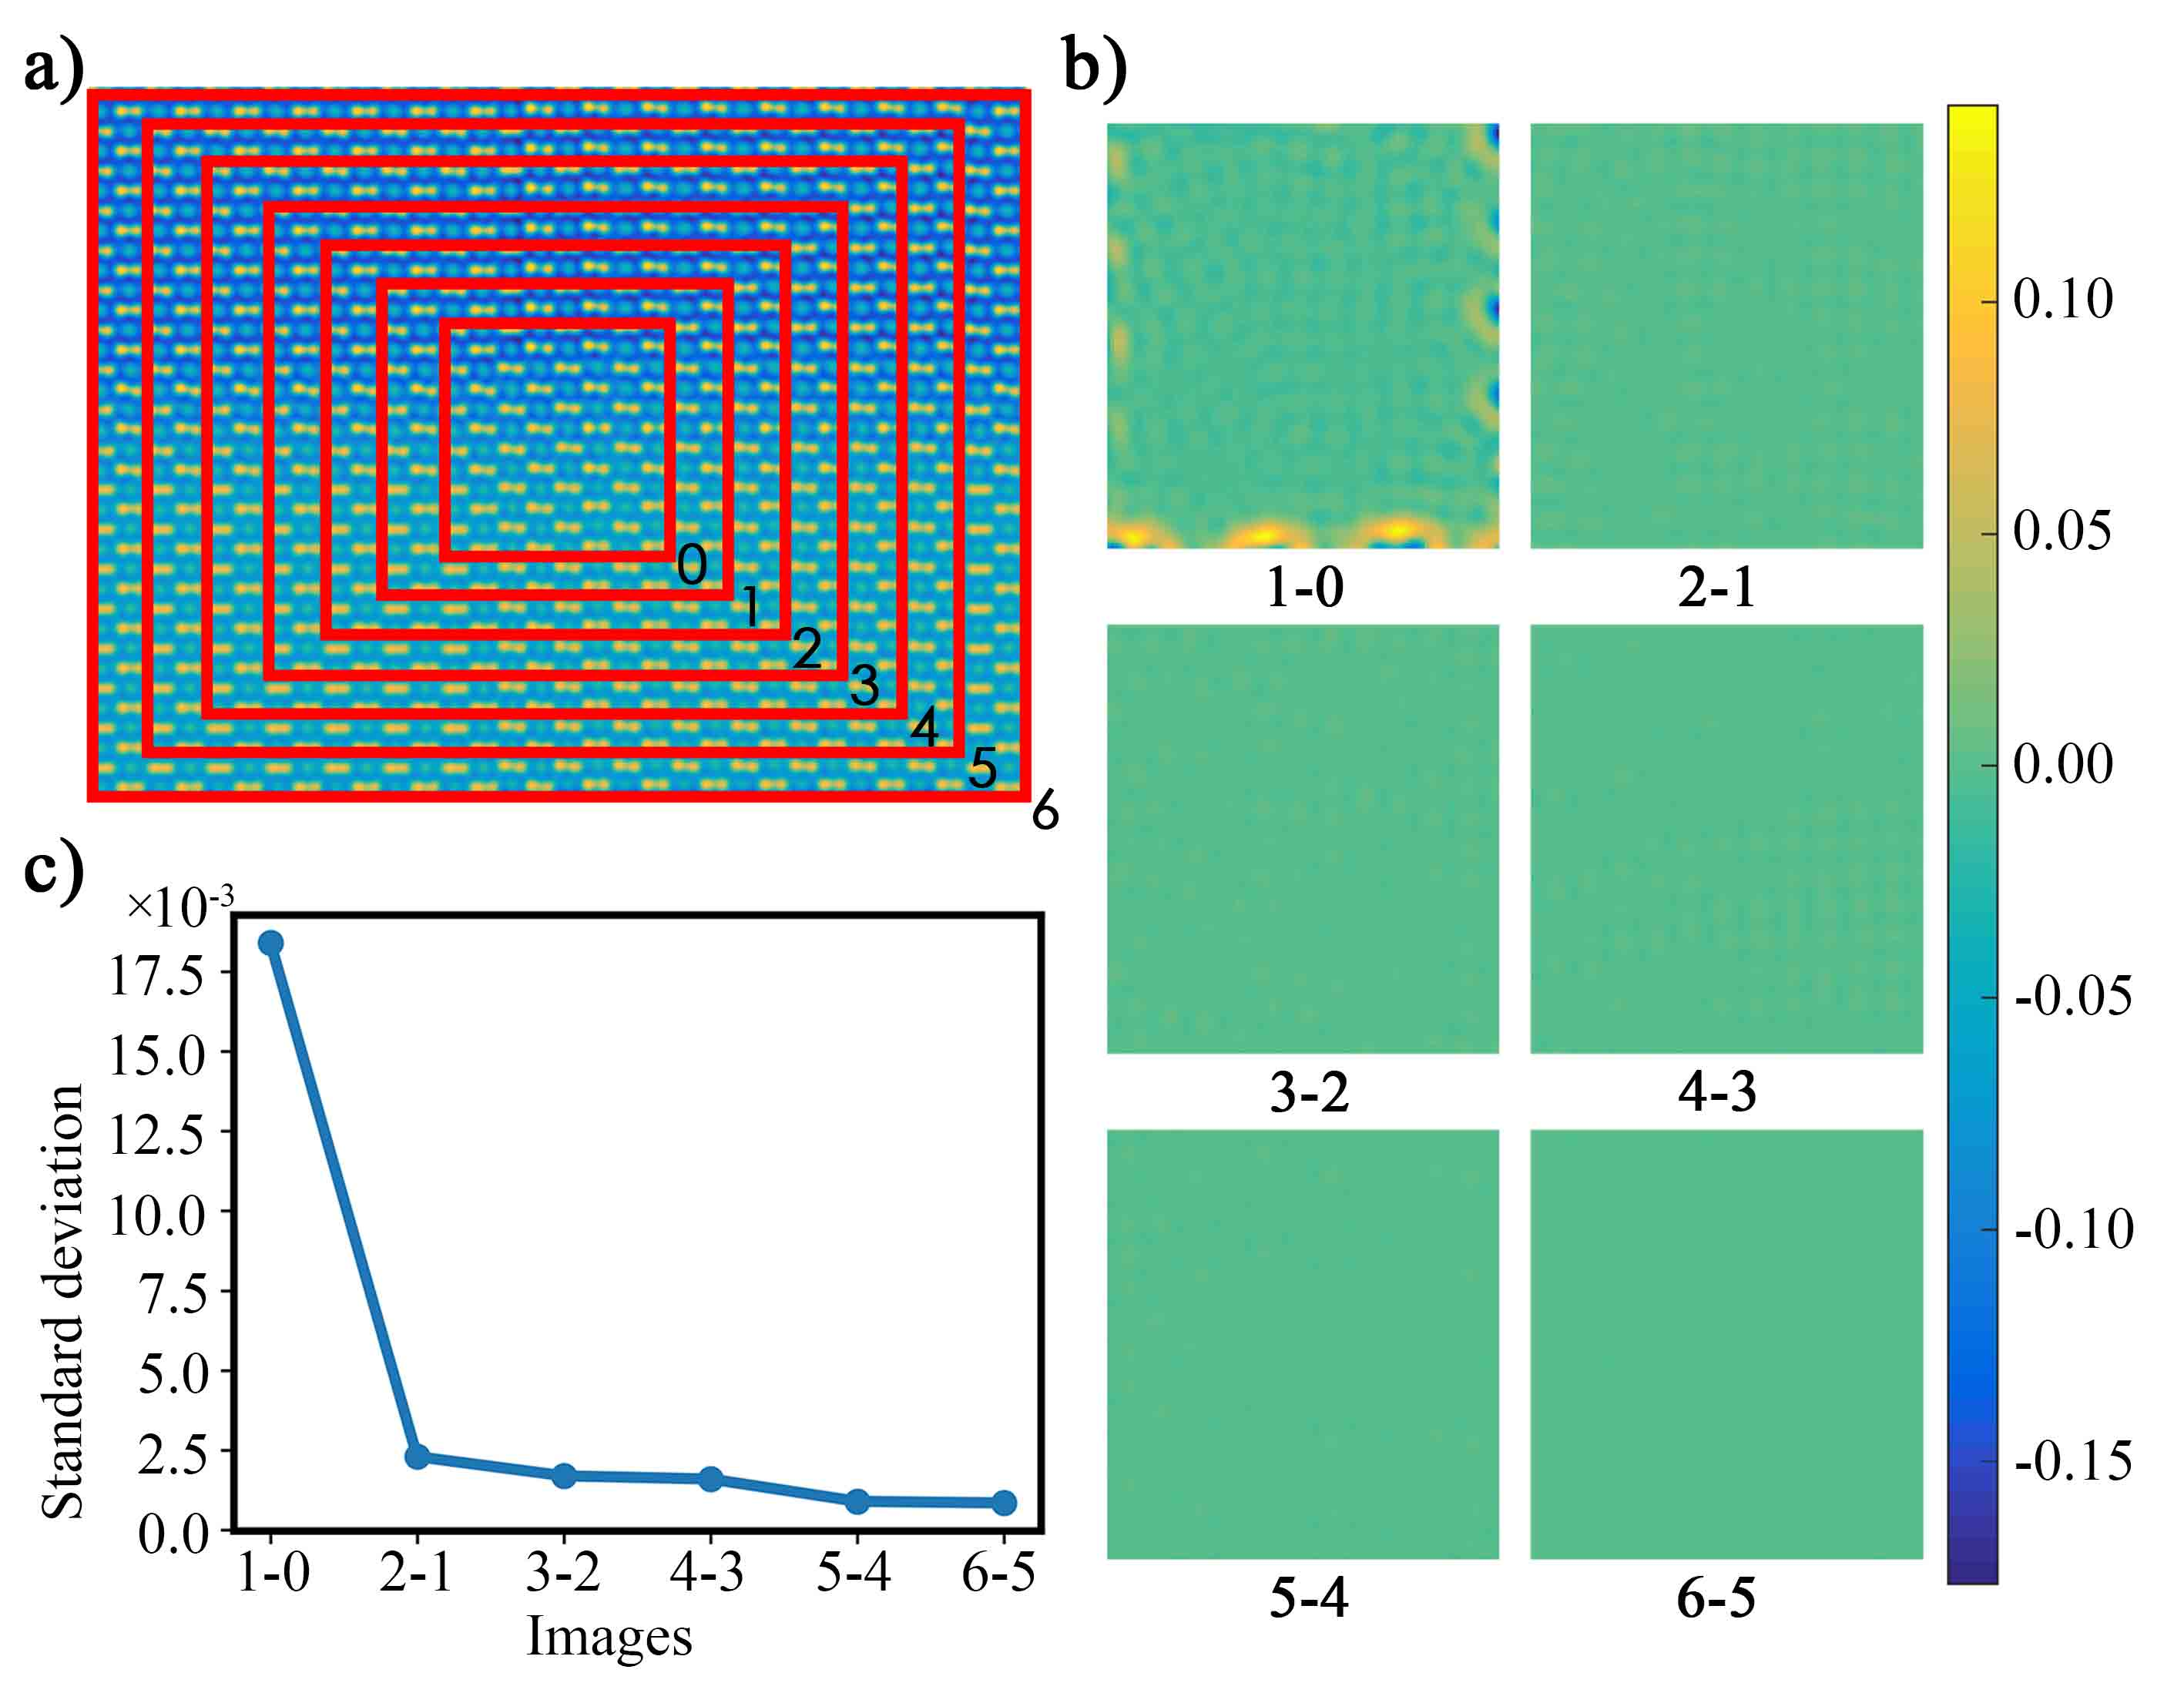
\includegraphics[width=0.8\textwidth]{../2.8/28}
	\caption{环绕效应收敛测试示意图}\label{fig:28}
	\song\tuzhu{a) 表面倾斜的 Si 超胞的模拟像,其中红色矩形框标记了不同尺寸的超胞,超胞 \textbf{0} 至超胞 \textbf{6} 尺寸依次增大;b) 两个连续超胞的模拟像的差,图像仅在超胞 \textbf{0} 所在的区域进行对比;c) 图 b 中每张图像的标准差的变化曲线}
\end{figure}

\subsection{自洽性验证及分辨率}
我们引入了一个自洽性验证方案以保证全局匹配算法结果的有效性,并且定义了三维重构在 $z$ 方向上的分辨率。通过自洽性验证方案得到的结果将更为客观,操作者对结果的影响程度将大幅降低。该方案的主要思想如图 4.10 所示,在实际三维重构时,即使所需重构的感兴趣区域已经确定,仍然存在许多种超胞的选取方式,即可选区不同的实验图像区域。比如,图 4.10 中红色矩形框所围的区域 A1(右上角标记)是一种超胞的选取方式。其他还存在一些相同尺寸的超胞选取方式,比如 A2,A3,B1,B2 等。问题的关键是,不同的超胞可能会导致最终重构的感兴趣区域的原子结构略有不同。这是因为同一个感兴趣区域在不同的超胞中具有略微不同的环境,这有可能导致不同的重构误差。举例来说,用全局匹配算法重构感兴趣区域(图 4.10 中橙色区域)时,由超胞 A1 重构所得的结果和由超胞 C5 重构所得的结果,有可能会略有差别。因为除了图 4.10 中的黄色区域是 A1 和 C5 共有的区域外,它们在其他区域具有不同的局部样品厚度、欠焦量以及非晶覆盖状况等。这种环境的差异会造成最终重构结果的差异。所以,原则上某一感兴趣区域的重构应该综合多个独立的重构结果,最终的重构结果应该是这些不同的重构结果的平均。如此所得的平均结果更加客观,消除人为操作对结果的影响,而且可以验证重构结果的合理性。
比较感兴趣区域中每一个原子柱的平均厚度和平均高度和每个独立重构结果的差别可以获得厚度和高度的重构误差。通过统计所有独立重构的结果中所有原子柱处的误差,我们可以以如下的方式定义三维重构在 $z$ 方向上的分辨率:首先去除所有误差中前 20\% 的较大误差,然后将剩余的 80\% 的误差中的最大值定义为三维重构在 $z$ 方向上的分辨率。比如,如果在对某一感兴趣区域的重构中产生的所有误差中,有少于 20\% 的误差大于或等于 2 个原子间距,而超过 80\% 的误差都小于 2 个原子间距,则定义该三维重构在 $z$ 方向上的分辨率是 1 个原子间距。
\begin{figure}[htbp]
	\vspace{\baselineskip}
	\centering
	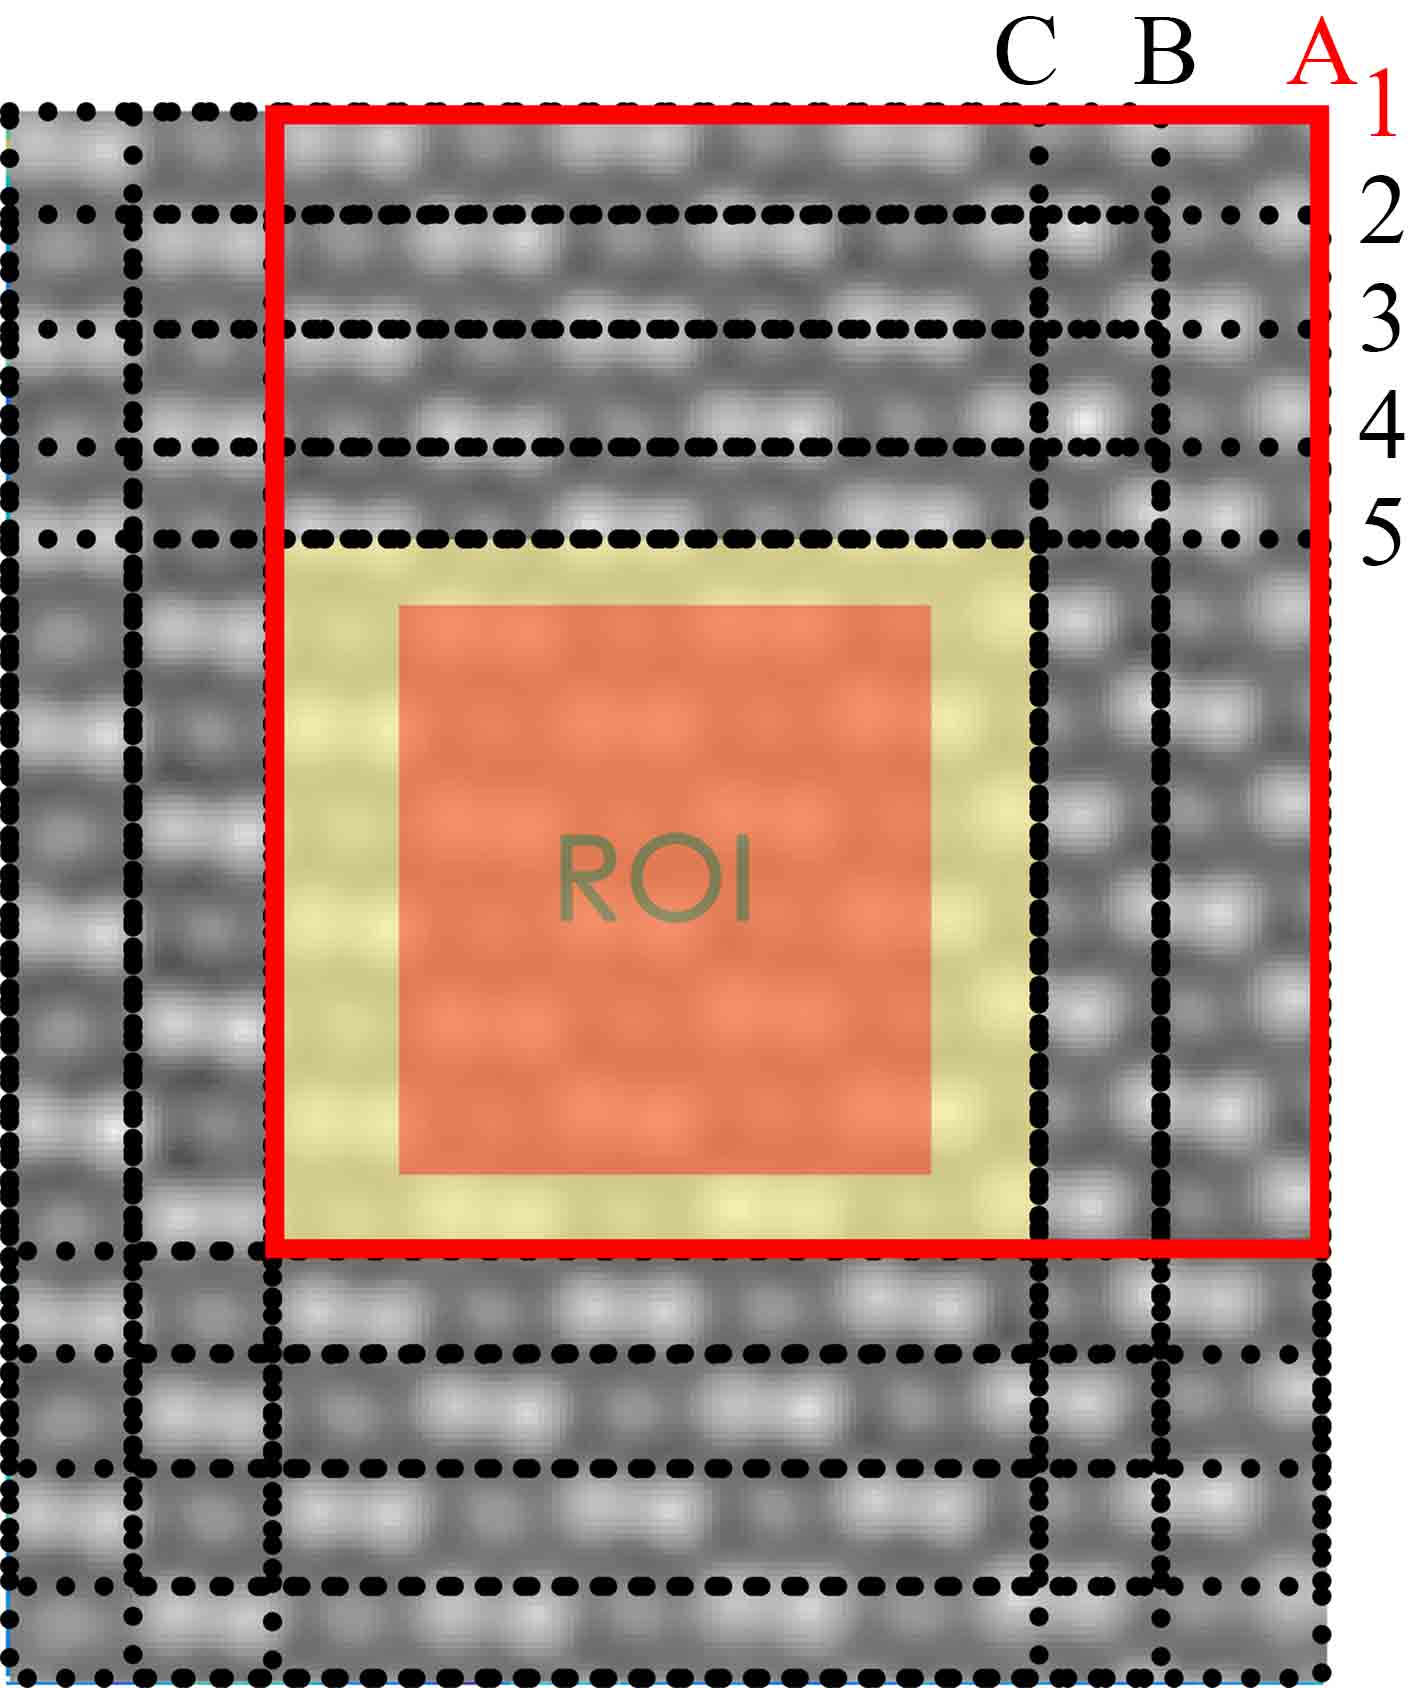
\includegraphics[width=0.4\textwidth]{../2.9/29}
	\caption{自洽性验证方案分区图}\label{fig:29}
	\song\tuzhu{图中展示了相同尺寸但是位置不同的超胞 A1, A2 … C5 的选区方式,这些超胞均具有相同的公共区域,右上角是不同超胞的命名方式}
\end{figure}

\subsection{非晶对重构的影响}
由于非晶对样品的污染在大部分的实验中是不可避免的,但是又无法将其考虑到重构的过程中,因此有必要定量估算其对图像衬度的影响。为了模拟非晶对一般晶体材料高分辨电镜照片图像强度的影响,我们构建了一个尺寸为 $9.7 \textnormal{ nm} \times 9.7 \textnormal{ nm} \times 4.3 \textnormal{ nm}$ 的 Si  超胞。如图 4.11d 所示,该超胞的 $z$ 方向沿晶体的 [100] 方向,在晶体上下表面分别为其覆盖上厚度为 0.0,0.5,1.0,1.5,2.0 以及 2.5 nm 的非晶层。其中 Si 非晶层中的原子位置是通过分子动力学模拟软件 LAMMPS,根据 T. Grieb 等工作~\cite{Grieb2018}中的方式计算所得。图 4.11a-c 直观地展示了当表面非晶层增厚时,所得的高分辨电镜照片的图像衬度变化之明显。图 4.11e 进一步展示了由非晶层导致的图像强度误差相对于非晶层厚度的变化曲线。从以上的对比可知,非晶对图像强度的影响是非常显著的,所以这些影响必须被仔细地分析以保证重构算法可以被正确地应用于实际材料的重构。值得注意的是,由于被非晶影响的高分辨电镜照片的噪音比较严重,在将这些照片与单纯晶体的高分辨电镜照片对比之前,这些照片都通过了 Weiner 滤波器~\cite{Kilaas1998}的过滤(电镜照片定量分析中经常执行的一个步骤),以减轻噪音的影响。实际上,Weiner 滤波器是一种在倒空间中去除图像背底噪音和提高图像质量的方法,它并不能完全消除非晶对图像衬度的影响,比如图 4.11b 和 c 与图 4.11a 依然具有很大的差别。

\begin{figure}[htbp]
	\vspace{\baselineskip}
	\centering
	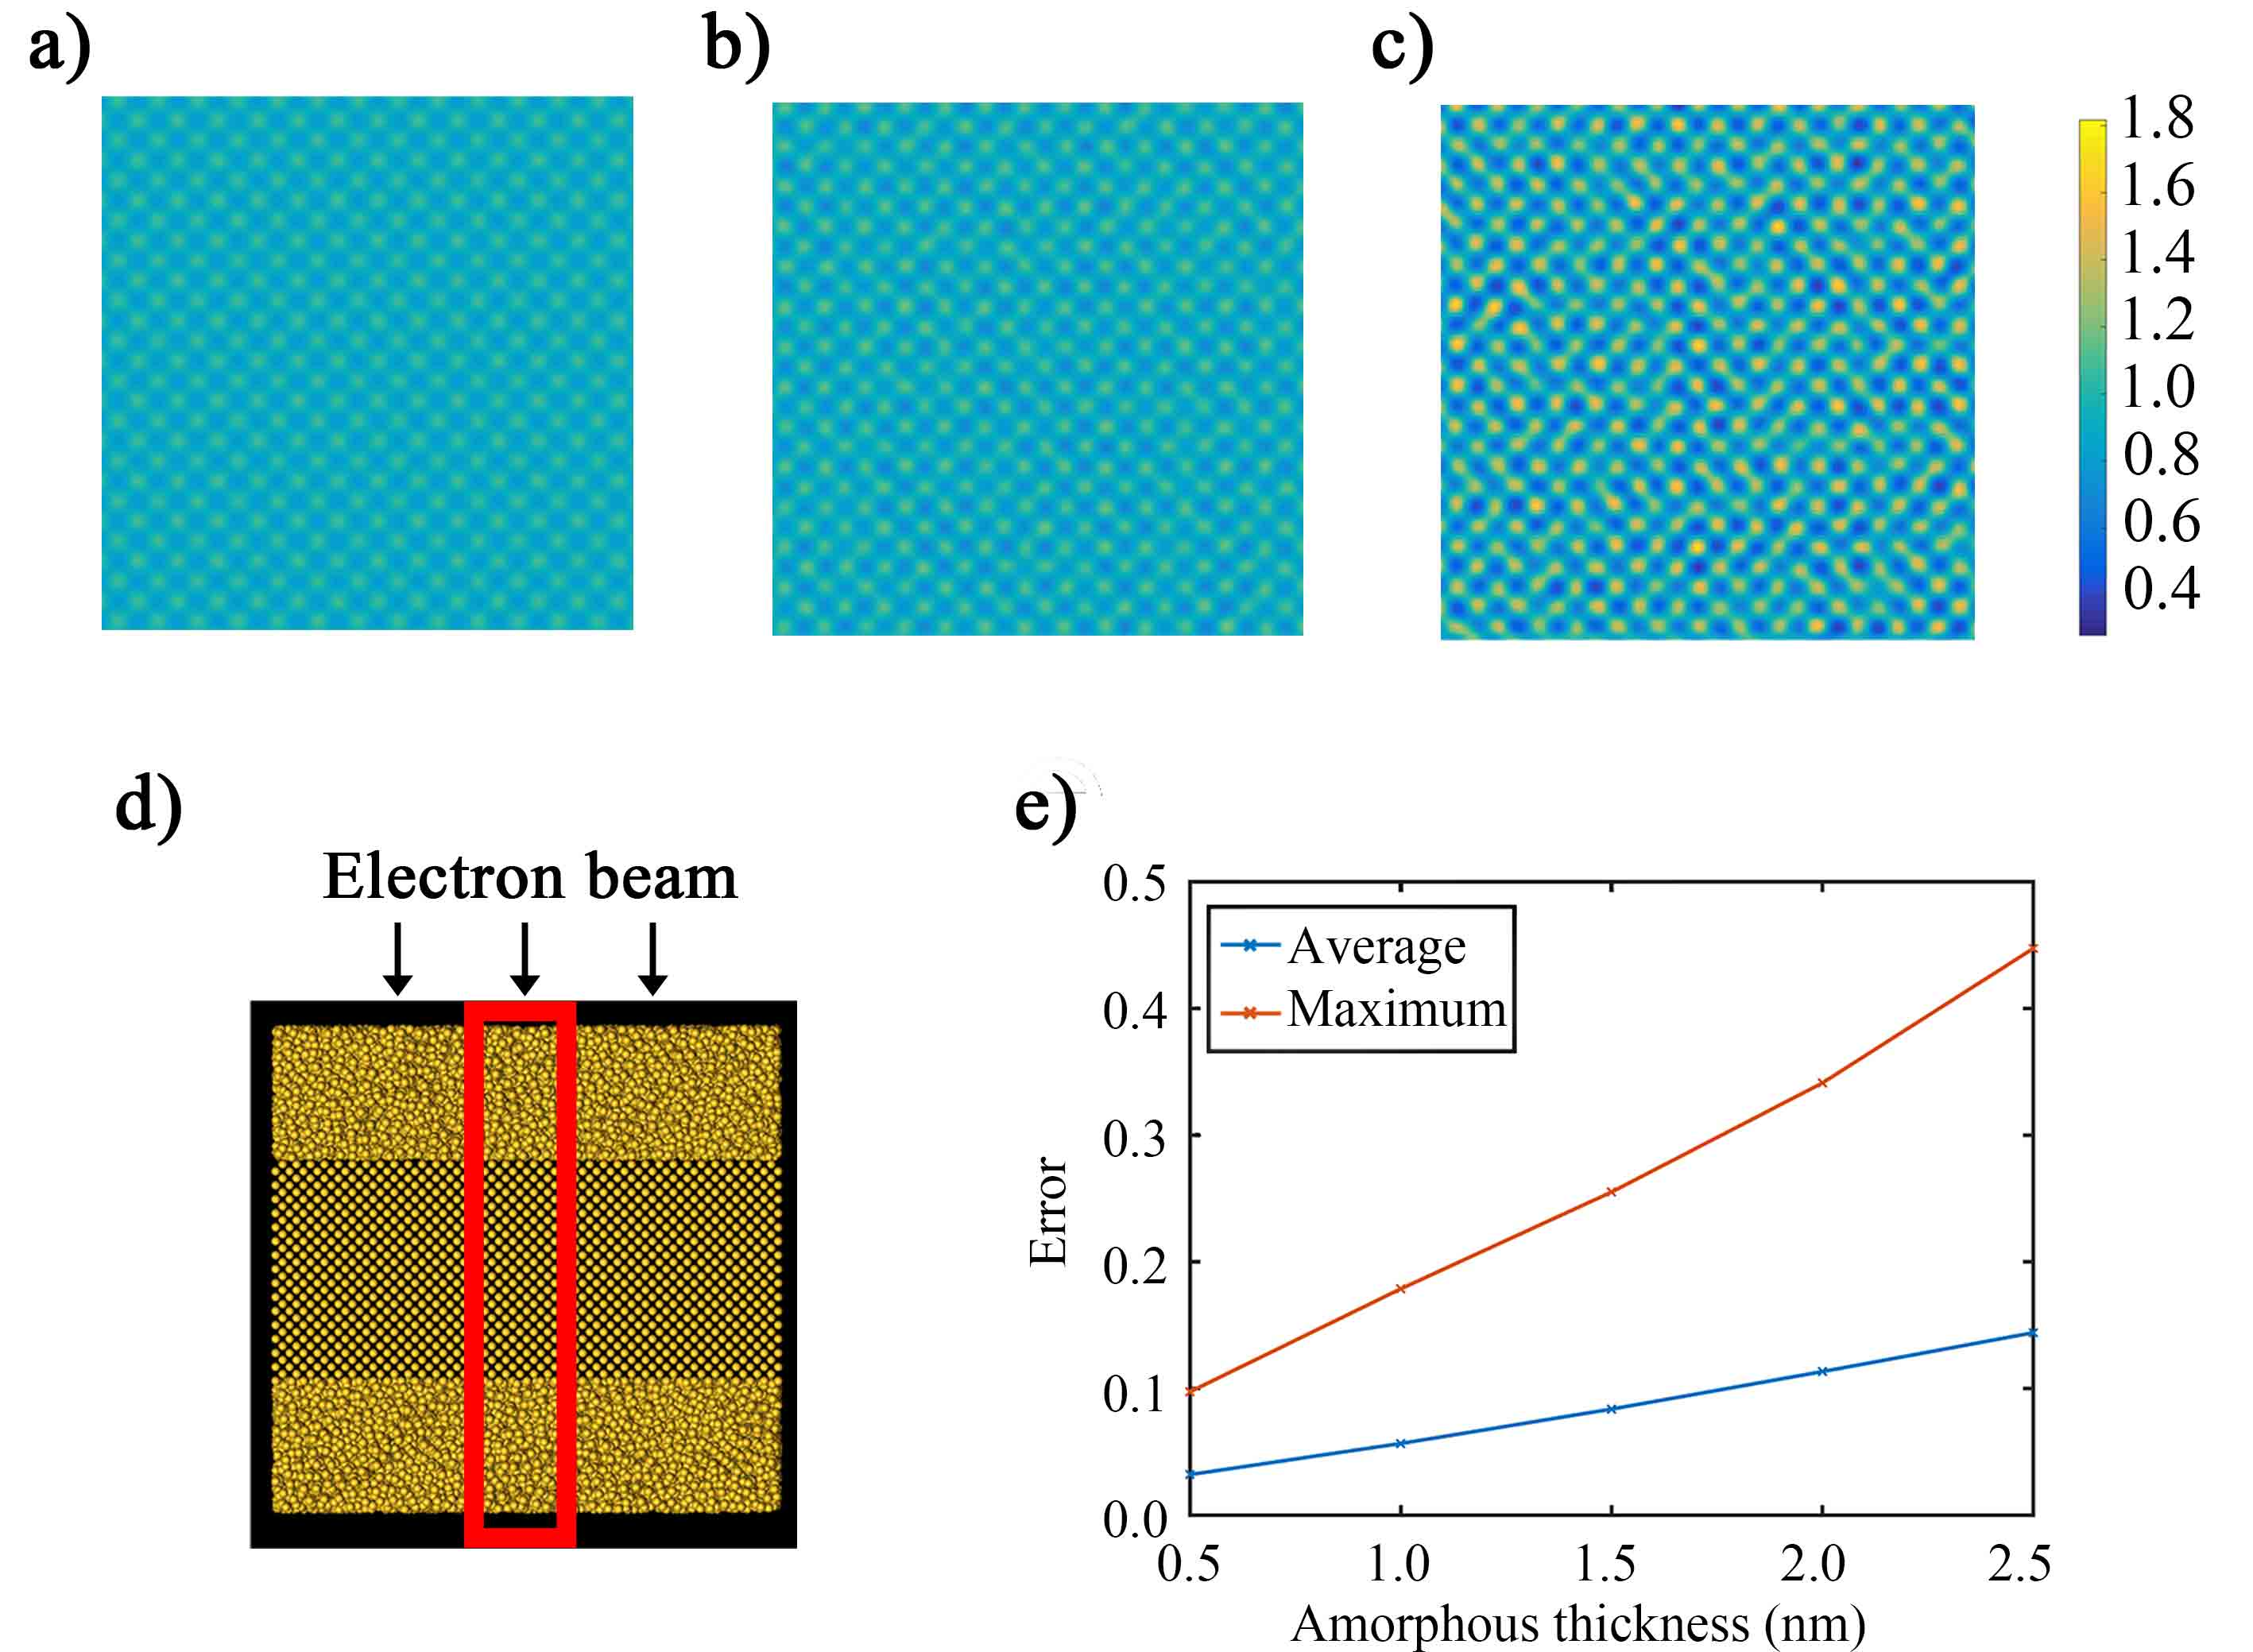
\includegraphics[width=0.7\textwidth]{../2.10/210}
	\caption{非晶对图像衬度的影响}\label{fig:210}
	\song\tuzhu{a-c) Si[100] 的高分辨电镜照片模拟像,其中 Si 晶体的上下表面覆盖了厚度为 0.0,0.5,2.5 nm 的非晶层,这些图片均通过 Weiner 滤波器过滤;d) Si[100] 样品的截面图,Si 晶体上下覆盖了等厚的非晶层,其中 Si 晶体的尺寸为 $9.7 \textnormal{ nm} \times 9.7 \textnormal{ nm} \times 4.3 \textnormal{ nm}$,电子束沿 Si[100] 入射,只有红色矩形框中的区域的模拟像展示于图 a-c 中;e) 覆盖非晶后的超胞的模拟像与 Si 晶体模拟像之间的平均误差与最大误差相对于非晶厚度的变化曲线}
\end{figure}

如图 4.11e 所示,当非晶层增厚时,最大误差增长的幅度比平均误差增长的幅度更大,所以其中大误差的具体分布情况需要进一步的分析。图 4.12a 和 b 展示了当非晶厚度为 0.5 nm 时,大误差(红色标记所示,绝对值超过 0.1)相对于 Si[100] 投影势场的分布情况。从中可以发现,当非晶层较薄时,其引入的大误差大部分分布于原子柱之间,只有小部分的大误差分布于接近原子柱的位置。从图 4.12c 和 d 中的误差分布直方图可知,当非晶层很薄时(比如 0.5 nm),其产生的误差几乎不超过 0.1。但是当非晶层厚度增加至 2.5 nm 时,其引入的误差大部分都会超过 0.1,此时的误差将随机分布于整个区域。

\begin{figure}[htbp]
	\vspace{\baselineskip}
	\centering
	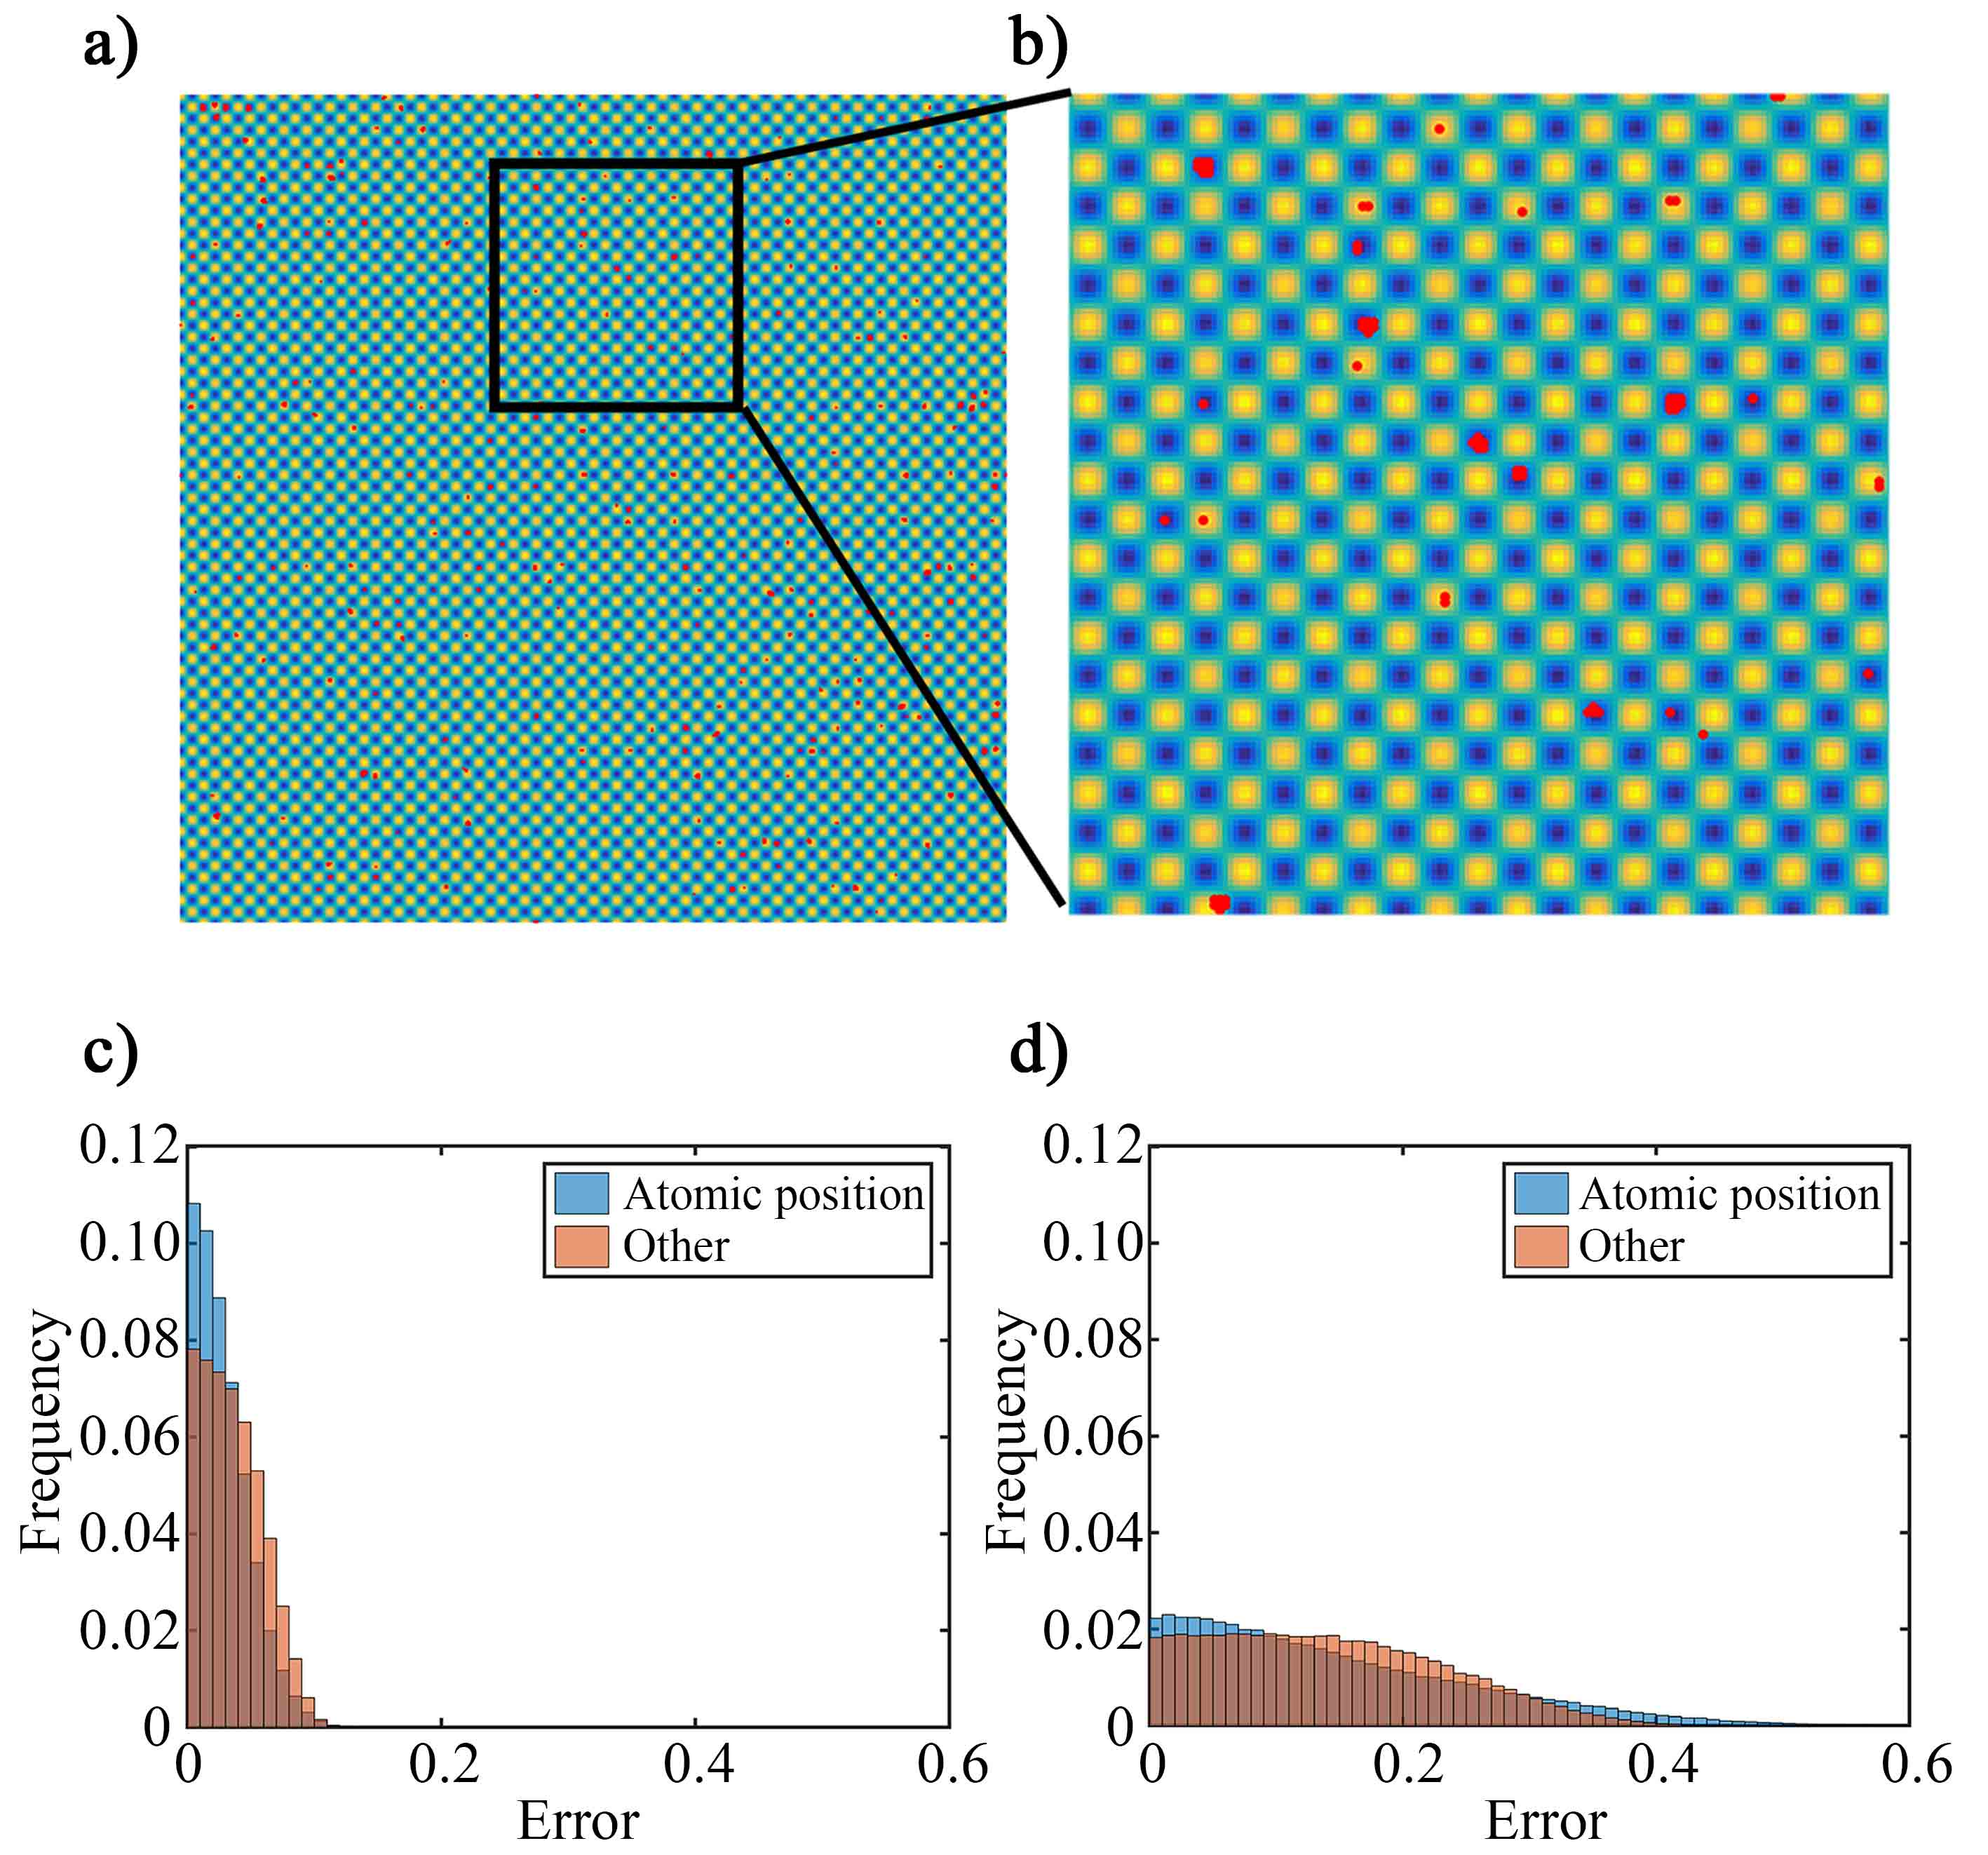
\includegraphics[width=0.9\textwidth]{../2.11/211}
	\caption{非晶引起的误差分布示意图}\label{fig:211}
	\song\tuzhu{a) 图 4.11a 与图 4.11b 之间较大误差的分布情况示意图,其中误差绝对值大于 0.1 的区域被标记为红色;b) 图 a 中线框区域的放大图;c,d) 图 4.11a 与图 4.11b 以及图 4.11a 与图 4.11c 之间的误差的分布直方图}
\end{figure}

\subsection{三维重构的置信度}
为了测量全局匹配算法重构的可靠性以及其对一般材料和一般原子分辨率图像的适用性,在此定义置信度 $C_{3D}$ 如下:
\begin{equation}
C_{3D}=1-E_{average}-E_{column}
\end{equation}
其中 $E_{average}$ 是整张图像的平均误差与整张实验图像的平均图像强度的比值,$E_{column}$ 是原子柱位置的平均误差与原子柱位置的平均图像强度的比值。实际上,第一项 $E_{average}$ 已经包含了第二项 $E_{column}$ 中的误差,但是原子柱位置的误差相比于原子柱位置之间的误差对重构结果的影响更大,所以将该类误差在置信度中的权重加倍。可以合理推断,误差越小,重构的置信度就应该越高。当误差全部由非晶引起时, $C_{3D}$ 直接与非晶层的厚度呈负相关,如图 4.13a 所示。随着非晶层由 0 增加至 $1.5 \textnormal{ nm}$,三维重构的置信度将从 100\% 快速下降到 90\% 以下。一个好的三维重构结果,它的置信度应该保持在 90\% 以上。



需要指出的是,尽管非晶污染是实际实验中最难以控制的误差来源,其他的因素,例如成像条件偏离最佳等等也是产生误差的原因。任何使图像质量变差的因素都将降低三维重构结果的置信度。再次强调,在估计置信度时,原子柱位置的误差应该被加倍考虑,因为此处的误差对重构可靠性的影响最严重。

\begin{figure}[htbp]
	\vspace{\baselineskip}
	\centering
	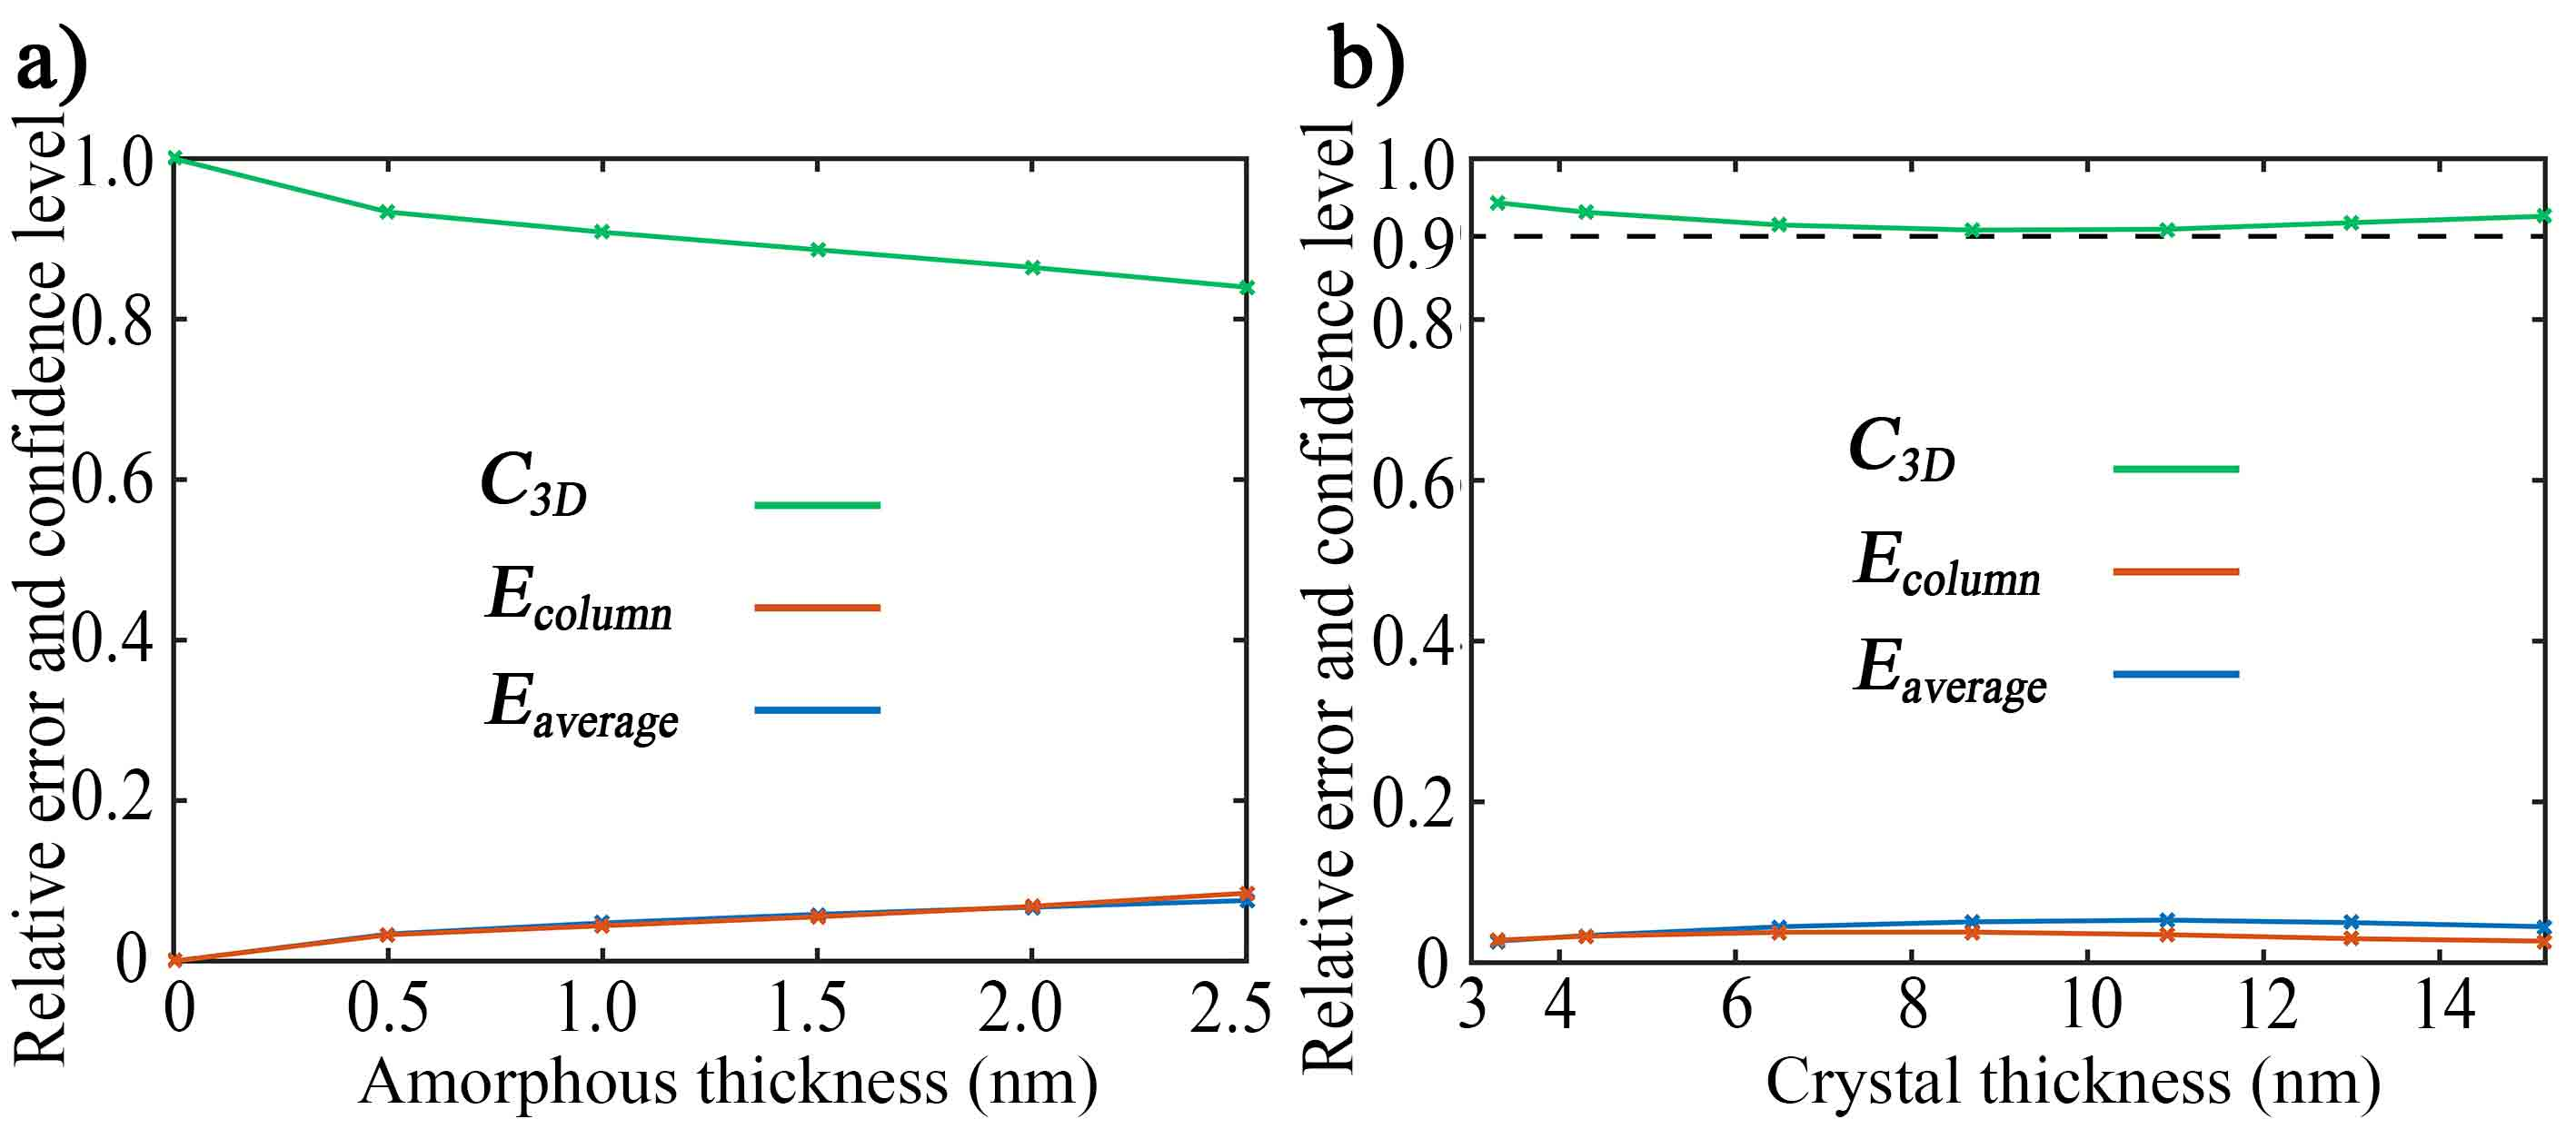
\includegraphics[width=0.9\textwidth]{../2.12/212}
	\caption{置信度关于非晶以及晶体厚度的变化关系}\label{fig:212}
	\song\tuzhu{a) 当晶体厚度为 4 nm 时,置信度关于非晶层厚度的变化曲线;b) 当非晶层厚度为 0.5 nm 时,置信度关于晶体厚度的变化曲线;所有的模拟都在球差和欠焦量都为 0 的条件下进行计算,所有误差均全部有非晶引起}
\end{figure}

\section{实验图像的三维重构}
在这一节中,我们将自洽性验证的三维重构方案应用于一张 Si[110] 的二维原子分辨率 TEM 照片,重构出了该样品的表面三维原子形貌,且重构获得了很高的分辨率和置信度。
\subsection{实验方案}
根据 C.H. Liu 等的研究~\cite{Liu2011},在 Al-Si 合金的热处理过程中,粗大的共晶 Si 颗粒的边缘会析出细小的纳米 Si 颗粒。这种纳米 Si 颗粒的尺寸非常小,适合 TEM 的观察,在球差矫正的高分辨 TEM 下可以拍摄得到高质量的原子分辨率照片。Al-Si 合金的 TEM 样品通过机械抛光和电解双喷制备,纳米 Si 颗粒出现在 Al 基体穿孔的边缘。用于观察 Si 样品的 TEM 型号是 Thermo Fisher FEI Titan 80-300 球差矫正 TEM。电镜照片沿 Si[110] 方向拍摄,详细的实验成像参数如表 4.3 所示。为了获得高质量的原子分辨率 TEM 照片,实验时使用了 NCSI 技术。$\textnormal{图 4.14a 和 b}$ 展示了拍摄到的实验照片,其中的亮点表示 Si 原子柱。在此图中,所有的 Si 原子柱在 $x-y$ 平面的位置都可以通过高斯拟合等方法确定~\cite{Garbrecht2011,Zhang2019}。相比于模拟像,该实验图像的噪音非常严重,这主要因为样品的表面存在一定的非晶污染。

\begin{figure}[htbp]
	\vspace{\baselineskip}
	\centering
	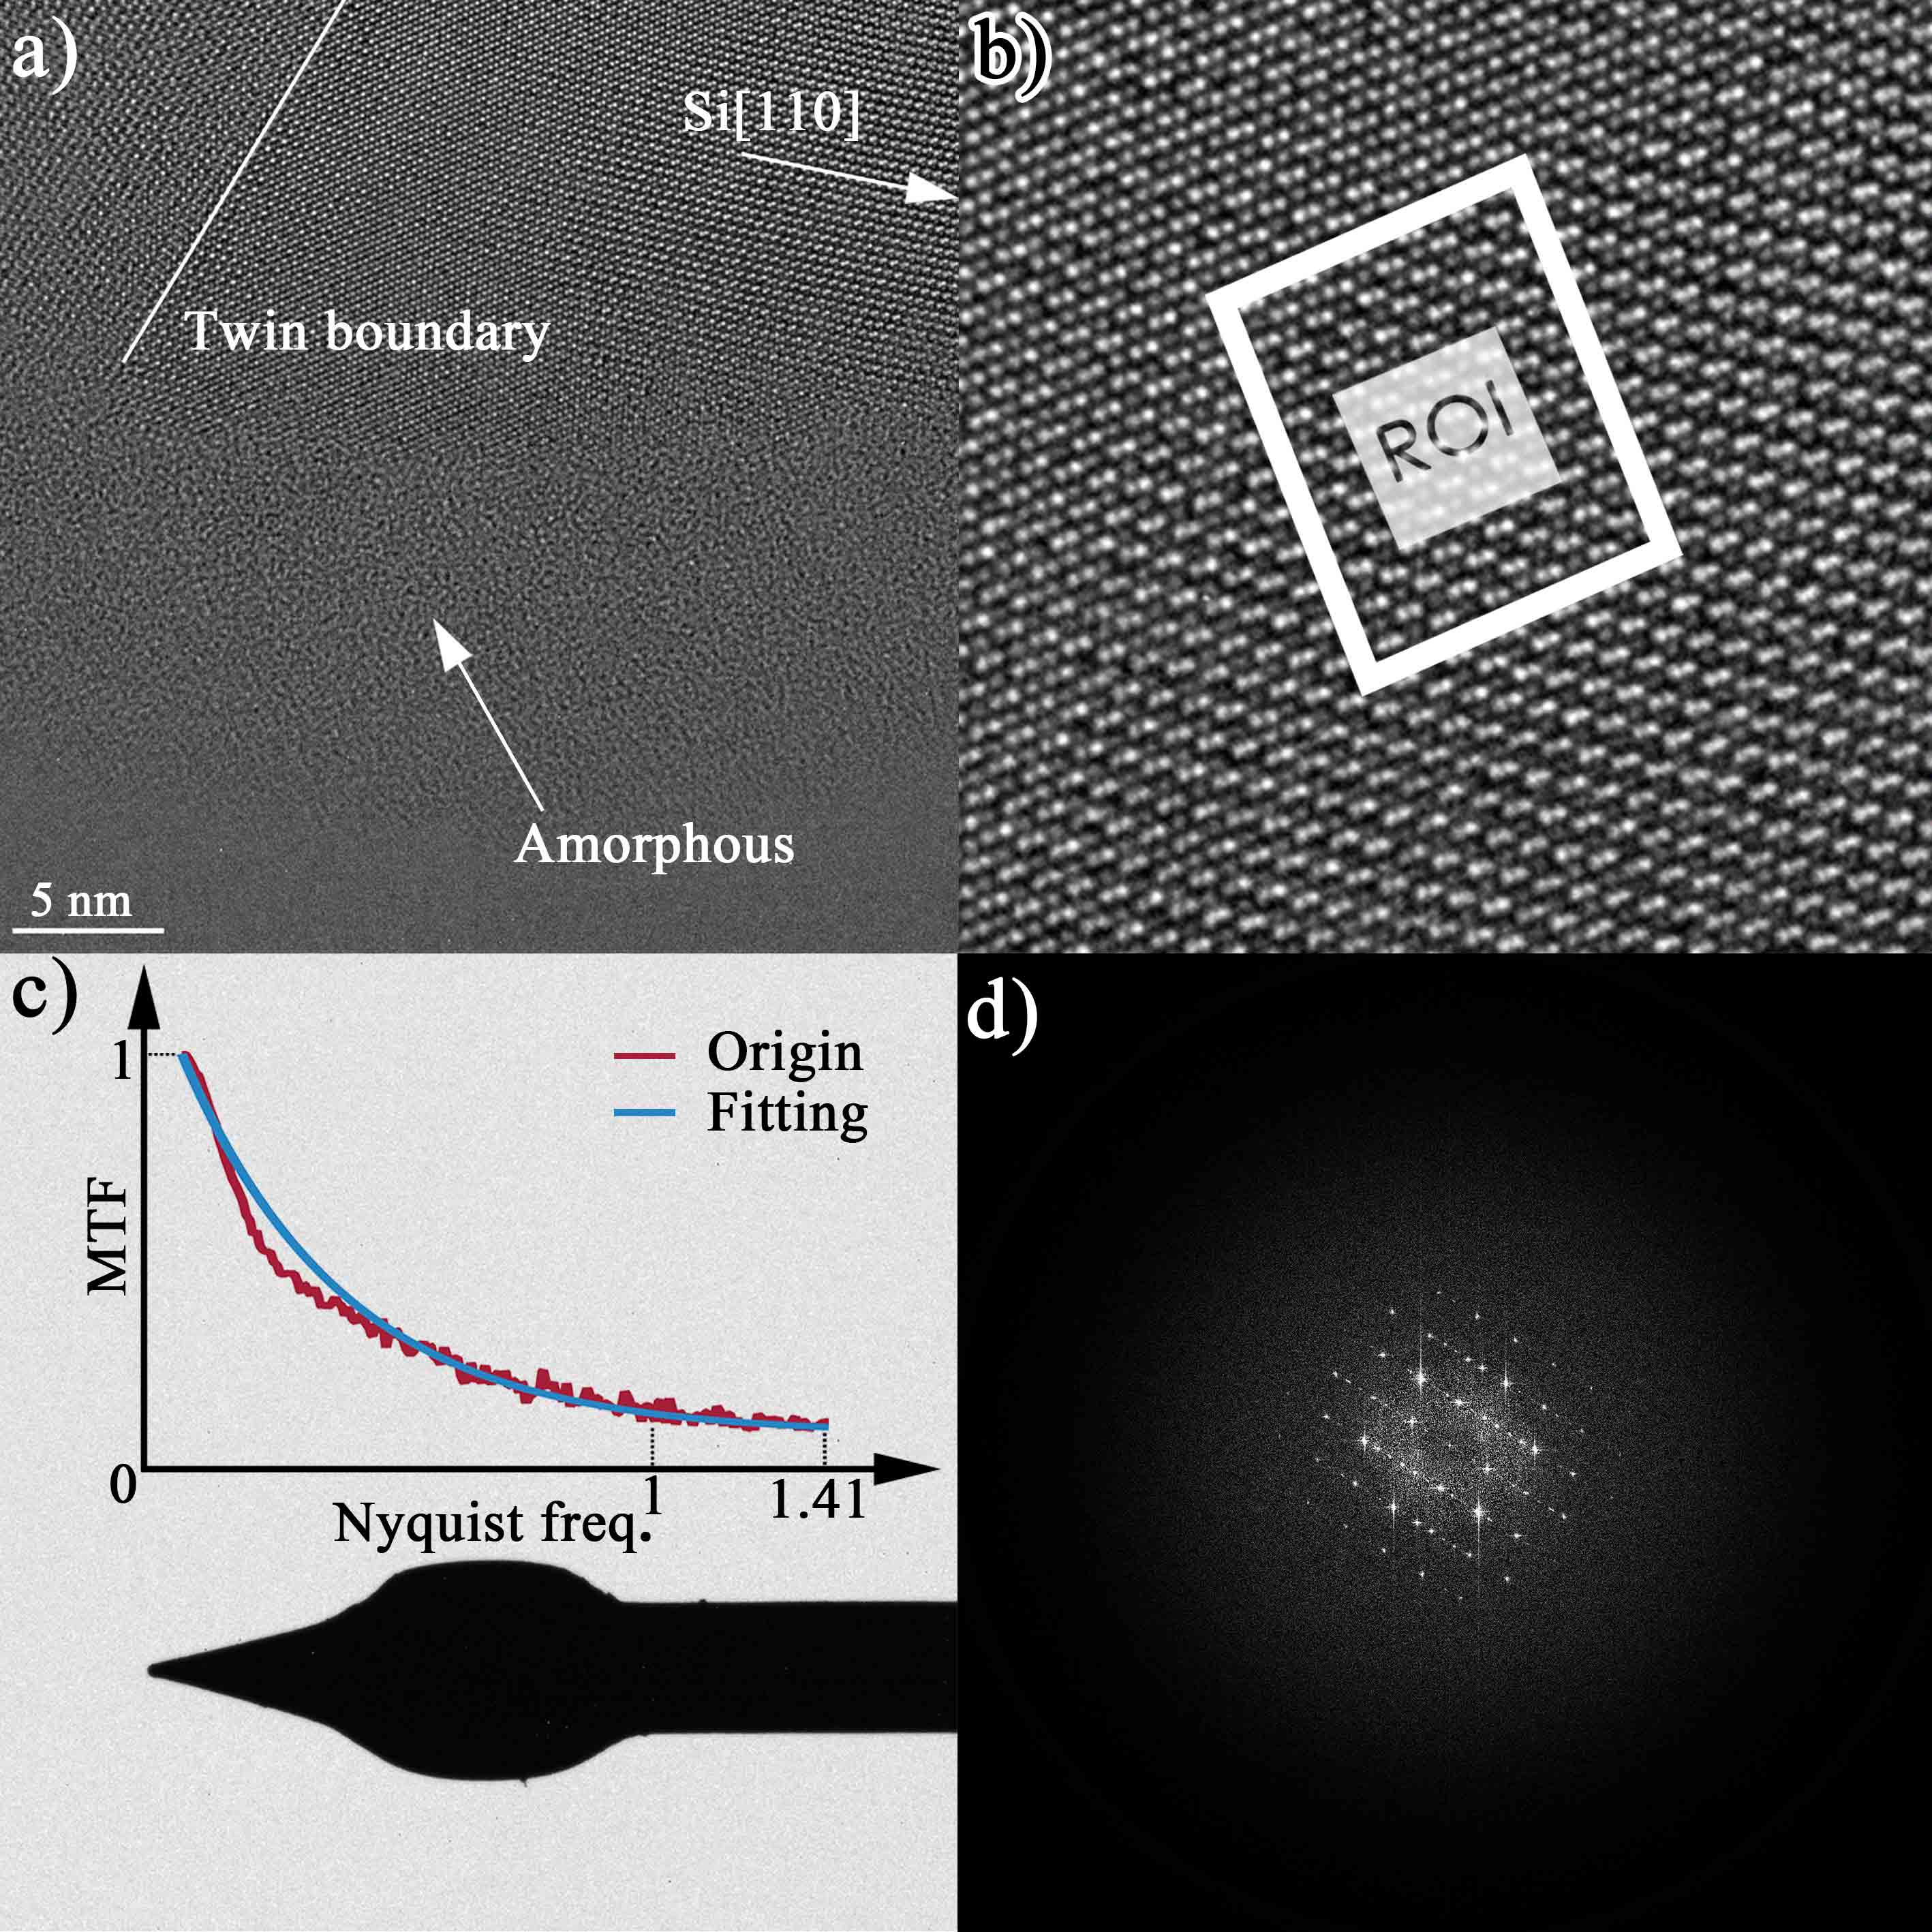
\includegraphics[width=0.85\textwidth]{../2.13/213}
	\caption{实验图像及其预处理}\label{fig:213}
	\song\tuzhu{a) 纳米 Si 颗粒的原子分辨率高分辨 TEM 照片;b) 图 a 中 Si[110] 区域的放大图,矩形区域是待重构的部分;c) 通过挡针像测量相机的 MTF,红色曲线是测量所得的 MTF 曲线,蓝色曲线是根据文献$^{[89]}$中的公式(13 )拟合的 MTF 曲线;d) Weiner 滤波后的 TEM 照片的傅里叶变换图}
\end{figure}

\quad

\begin{table}[htbp]
	\caption{高分辨 TEM 实验照片的成像参数}\label{tab:table1}
	\song\tuzhu\centering{其中 Cs$_3$ 表示三级球差,$\boldsymbol{A}_1$ 表示 2 阶像散,$\boldsymbol{A}_2$ 表示 3 阶像散,$\boldsymbol{B}_2$ 表示彗差,$\boldsymbol{A}_3$ 表示 4 阶像散, $\boldsymbol{S}_3$ 表示星差,$\boldsymbol{A}_4$ 表示 5 阶像散\\}
	\vspace{0.5em}\centering\wuhao
	\renewcommand{\multirowsetup}{\centering}
	\begin{tabular}{cccccccc}
		\toprule[1.5pt]
		Voltage & Cs$_3$ & \qquad$\boldsymbol{A}_1$\quad\quad & \qquad$\boldsymbol{A}_2$\quad\quad & \qquad$\boldsymbol{B}_2$\quad\quad & \qquad$\boldsymbol{A}_3$\quad\quad & \qquad$\boldsymbol{S}_3$\quad\quad & \qquad$\boldsymbol{A}_4$\quad\quad \\
		/kV & /mm & \quad/nm & \quad/nm &\quad/nm & \quad/nm & \quad/nm & \quad/$\upmu$m \\
		\midrule[1pt]
		\multirow{2}{1.3cm}{300} & \multirow{2}{1.3cm}{-0.0132} & \quad1.407 & \quad36.42 & \quad18.78 & \quad322.2 & \quad393.1 & \quad45.95\\
		& & \quad9.1$^{\circ}$ & \quad-38.1$^{\circ}$ & \quad-88.4$^{\circ}$ & \quad-19.1$^{\circ}$ &\quad-19.5$^{\circ}$ & \quad-11.6$^{\circ}$ \\
		\bottomrule[1.5pt]
	\end{tabular}
	\vspace{\baselineskip}
\end{table}

\subsection{图像预处理}
在进行定量分析之前,需要对实验图像进行预处理。首先需要排除 CCD 的 MTF 对实际图像强度的影响。在本研究中,MTF 是通过广泛使用的 knife-edge 方法~\cite{Thust2009}测量得到的。如图 4.14c 所示,这个方法使用电镜中的挡针锋锐的边界来测量 MTF。测量之后的 MTF 数据将根据拟合方法~\cite{VanBroek2012}进行计算得到拟合的 MTF 曲线,如图 4.14c 中蓝色曲线所示。之后将实验图像的傅里叶变换除以 MTF 以去除 MTF 对图像衬度的影响。图 4.15a 和 b 分别展示了原始实验图像和 MTF 矫正之后的图像,MTF 矫正后的图像的衬度略微提升。接着使用了 Weiner 滤波器降低图像中的噪音,降噪后的图像的傅里叶变换如图 4.14d 所示,降噪后的实验图像如图 4.15c 所示。最后将实验图像的图像强度归一化,否则无法与模拟像进行定量对比。归一化的方法是将实验图像的图像强度除以真空部位的平均图像强度~\cite{Hytch1994}。

\begin{figure}[htbp]
	\vspace{\baselineskip}
	\centering
	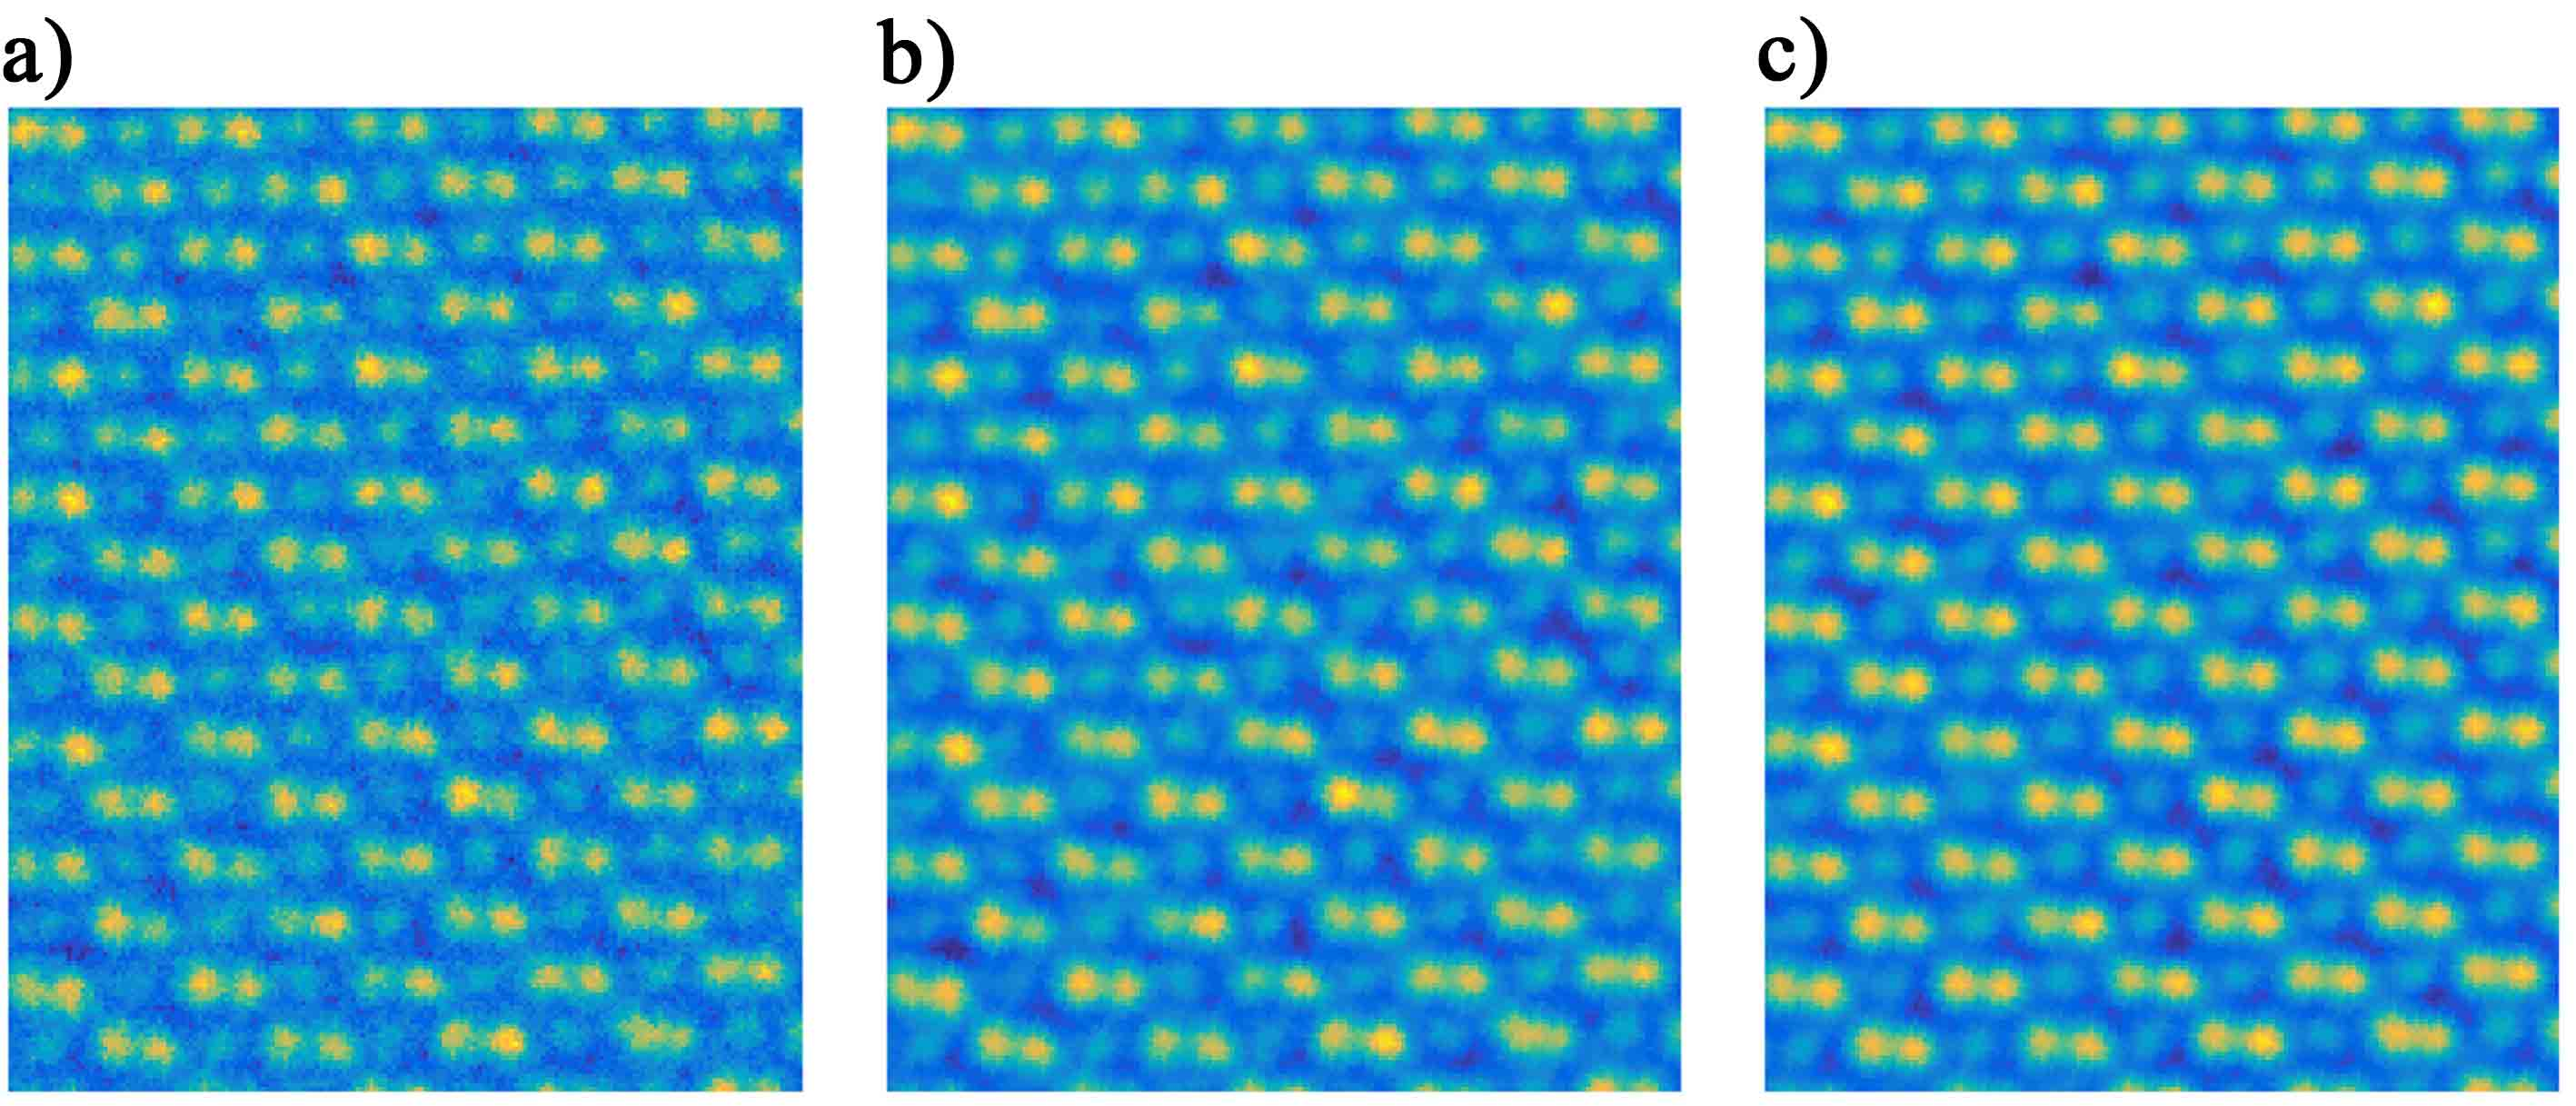
\includegraphics[width=0.9\textwidth]{../2.14/214}
	\caption{图像预处理过程中的图像变化}\label{fig:214}
	\song\tuzhu{a) 原始实验图像;b) MTF 矫正后的实验图像;c) 最后经过 Weiner 滤波后的图像}
\end{figure}

\subsection{三维重构过程}
为了定量对比实验像与模拟像的图像强度,必须选择正确的参数进行图像模拟。在本研究中,根据 H.X. Gao 等的研究~\cite{Gao1999},Si 原子的德拜沃勒因子取值为 $\rm{0.52\ \mathring{A}^2}$。且经过探究可知德拜沃勒因子的微弱变动对重构结果没有明显的影响。通过仔细的分析,在所选的待重构区域并没有观察到明显的晶体倾转。成像时的像差参数可参考表 4.3,由于实验时使用了球差矫正器,所以这些像差数值都非常小。由于样品中存在原子的弛豫和残余应力,实际 TEM 样品中的原子并不完全按照理想的 Si 晶体中的原子位置排列,所以每一个 Si 原子柱的位置都需要被精准地测量,并且反复对比实验像与模拟像以确定各原子柱的位置。图 4.16b 展示了测量的 Si 原子柱位置与理想的 Si 原子柱位置的对比图。




\begin{figure}[H]
	\vspace{\baselineskip}
	\centering
	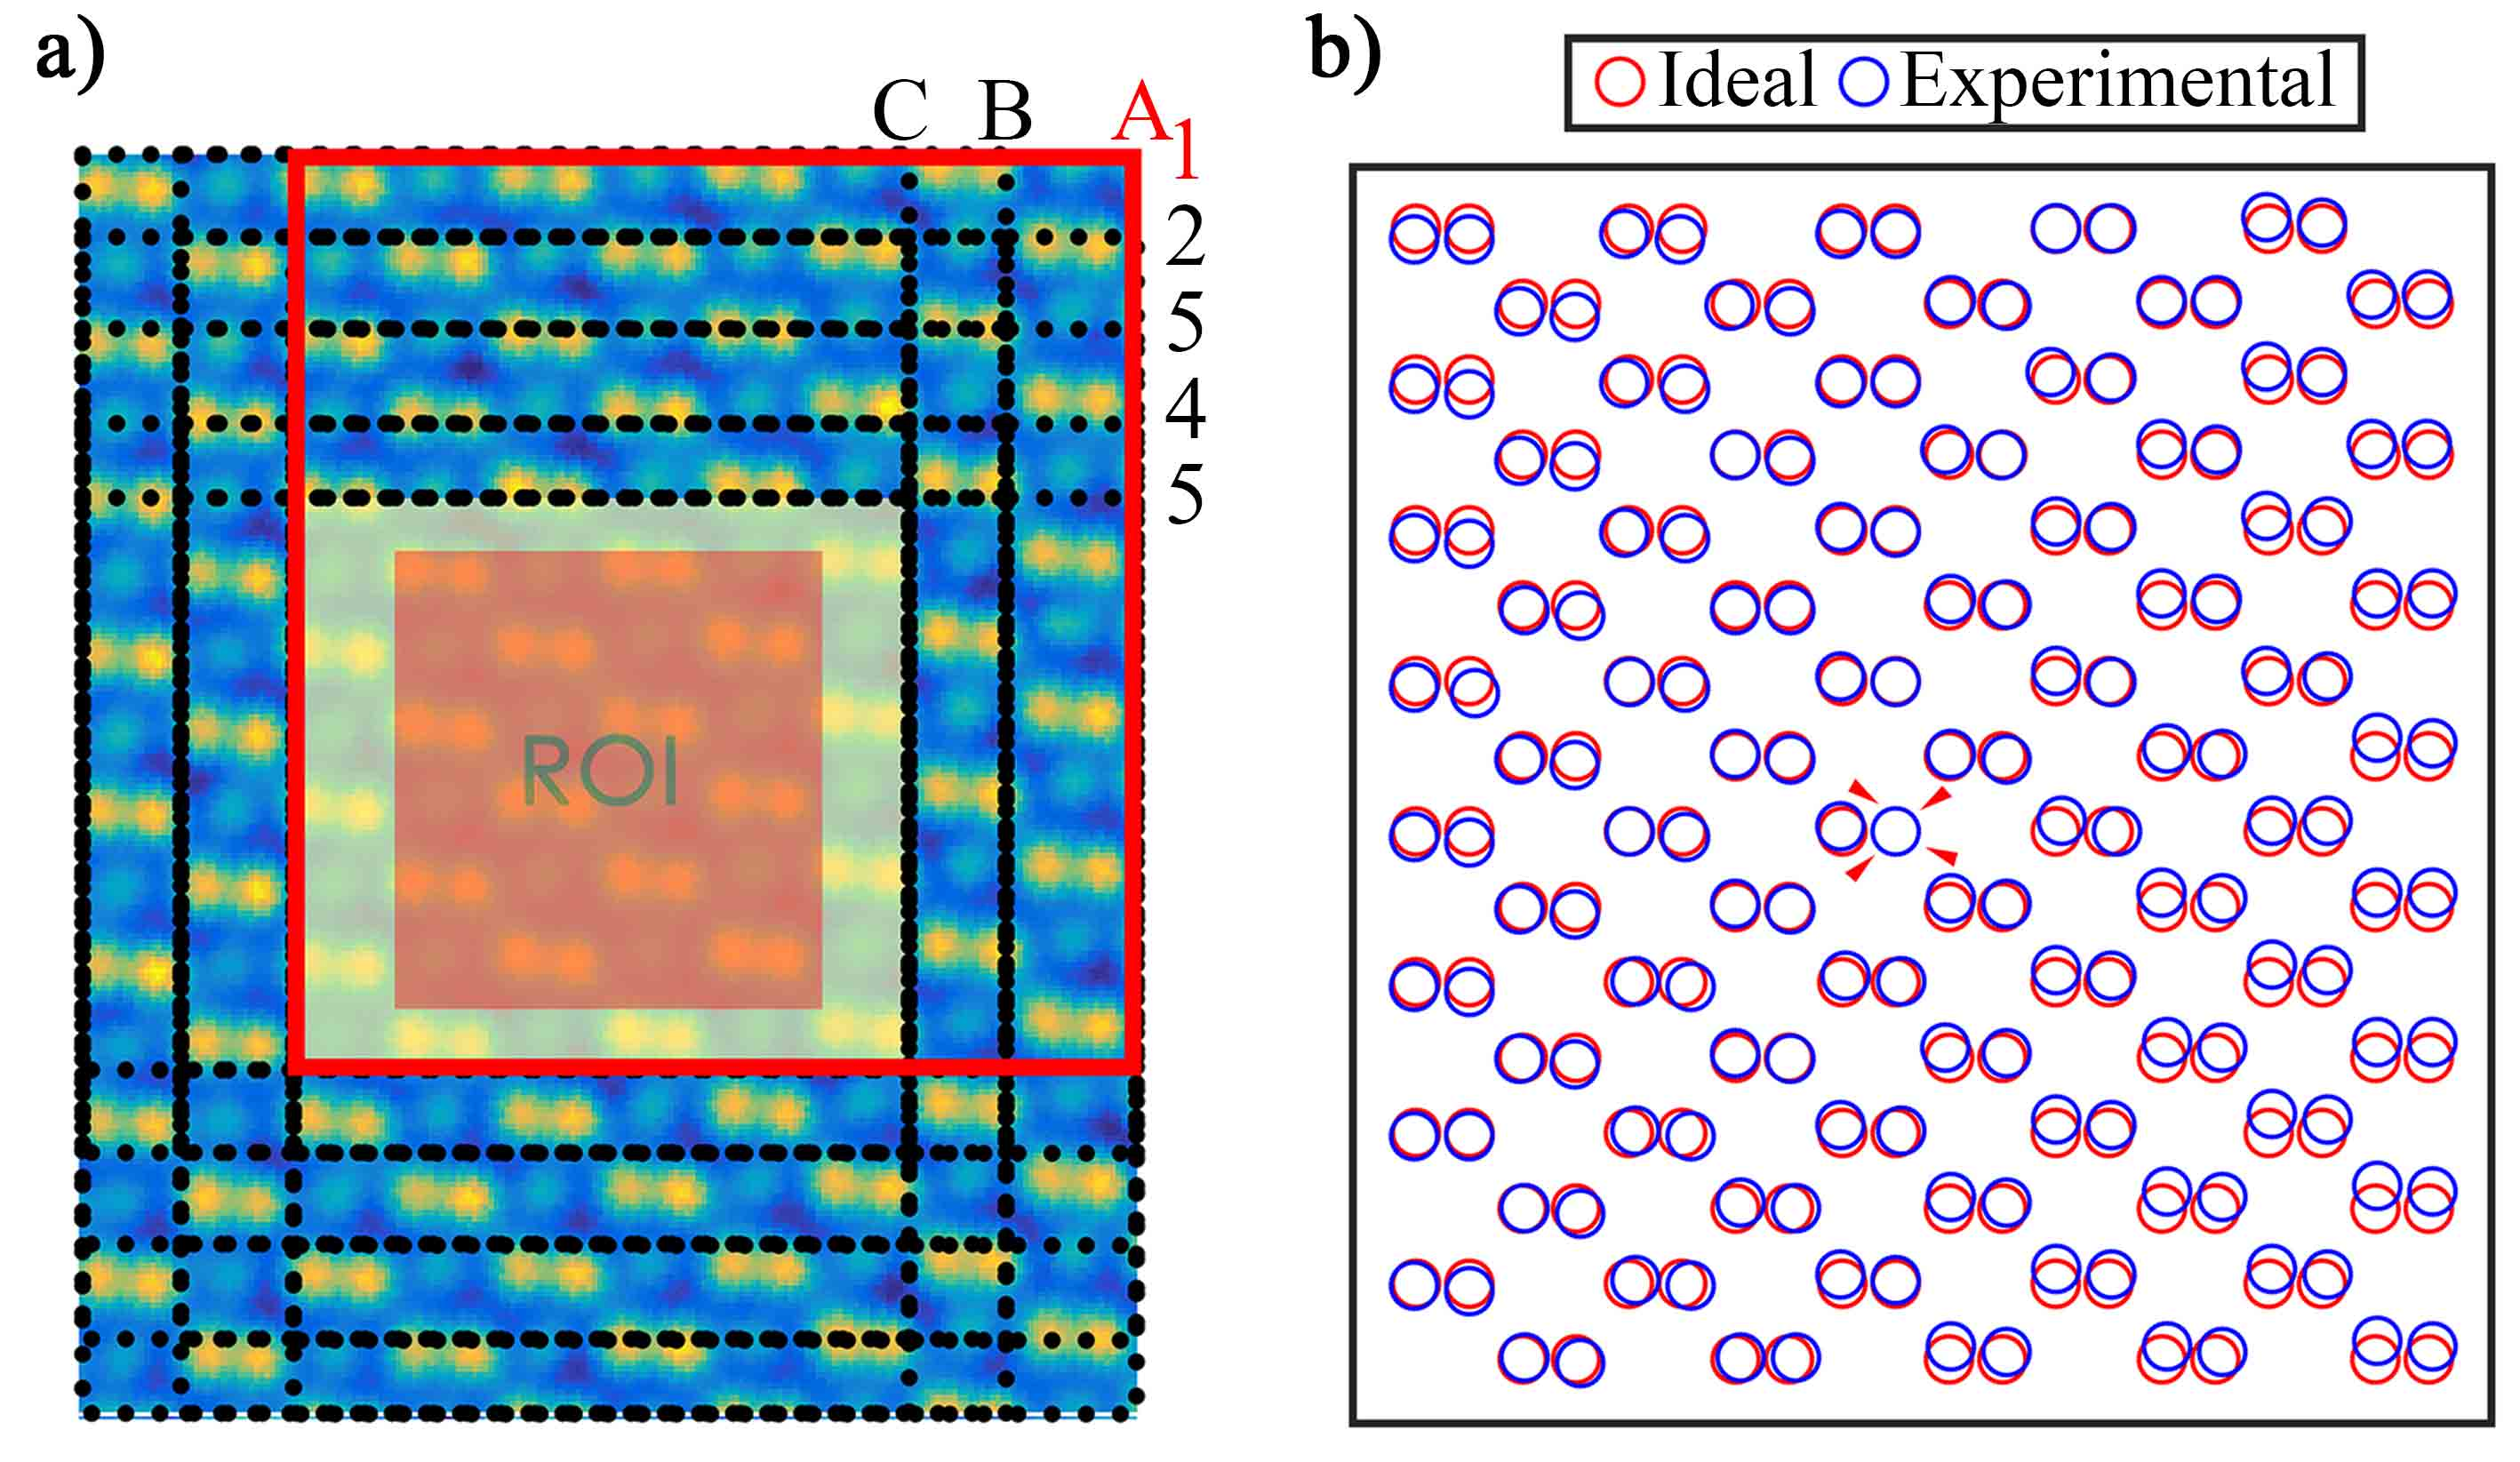
\includegraphics[width=0.9\textwidth]{../2.15/215}
	\caption{重构区域的划分以及 Si 原子柱位置的测量}\label{fig:215}
	\song\tuzhu{a) 待重构的实验图像,图中红色部分是感兴趣区域,A1,A2,…,C5 分别是 15 个相同尺寸的超胞,黄色区域是它们的公共区域,这些超胞将用于 15 次独立的重构;b) 理想晶体中的 Si 原子柱位置和实际测量的 Si 原子柱位置,中间红色箭头标记的是这两套原子柱位置的重合处}
\end{figure}

如第 4.3.2 条中所述,为了得到可靠的重构结果,需要采取自洽性验证方案,对同一个感兴趣区域进行多次独立的三维重构,最后通过统计数据定量分析三维重构的分辨率,以及得到最终的重构结果的置信度。在本次实验图像的重构中,如图 4.16a 所示,共选取了 15 个相同尺寸的单胞来重构中间的感兴趣区域。图 4.17a 展示了某三次重构的重构结果的上表面示意图,图 4.17b 展示了相应的下表示意图。观察可知,这几次重构的重构结果非常接近,但总是存在略微不同。图 4.17c 展示了重构的感兴趣区域的平均结果中每一个原子柱的厚度和高度。

为了估算三维重构 $z$ 方向上的分辨率,图 4.18a 和 b 统计了每一个 Si 原子柱的厚度以及高度的重构结果。其中橙色标记了各原子柱的平均结果。表 4.4 展示了 15 次独立重构各自的最大绝对误差。根据以上数据可知,全局匹配算法的稳定性很高,15 次重构的重构结果之间的差异很小。在原子柱厚度方面, 15 次重构结果的最大误差都是 1 个原子间距(0.384 nm);在原子柱高度方面,有 13 次(86.7\%)重构的最大误差是 1 个原子间距,其他 2 次(13.3\%)重构结果的最大误差是 2 个原子间距。因此,根据上文中提出的定义三维重构分辨率的原则,扣除前 20\% 的大误差,本次重构的分辨率在原子柱厚度和高度上均是 1 个原子间距,这意味着 Si 样品的表面形貌在原子分辨率下被重构了出来。

\quad

\begin{figure}[H]
	\vspace{\baselineskip}
	\centering
	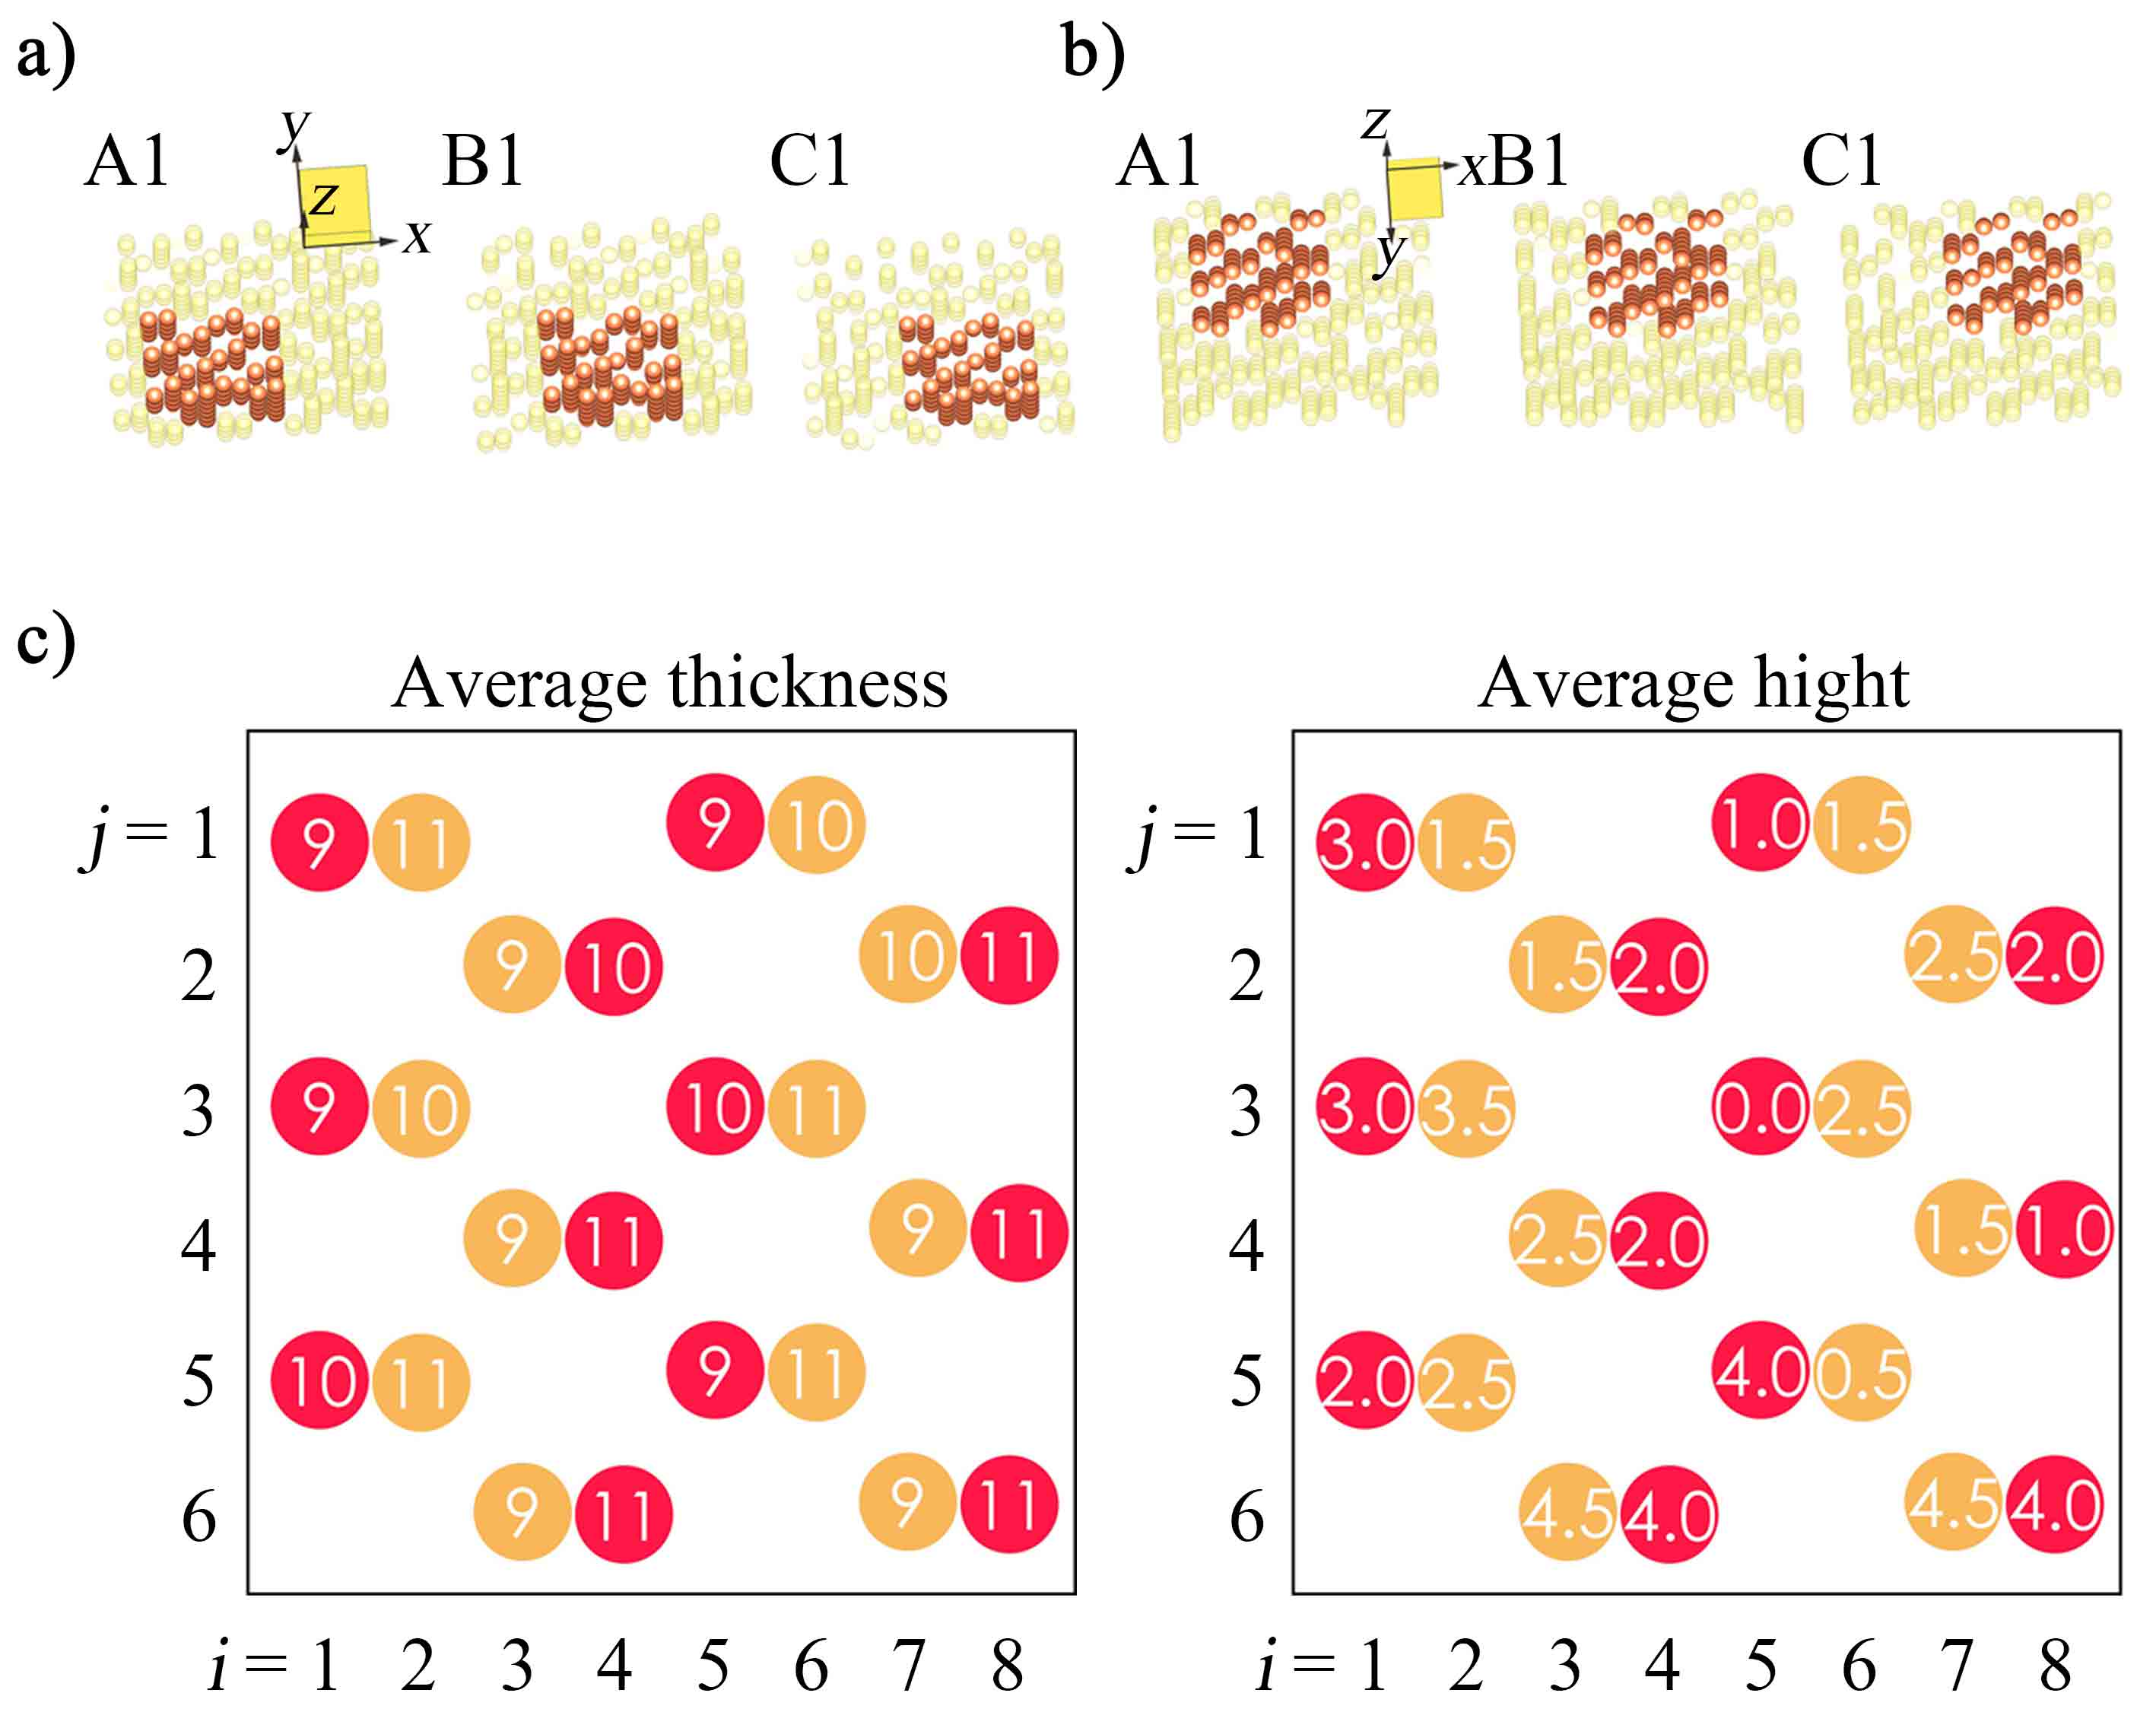
\includegraphics[width=0.9\textwidth]{../2.16/216}
	\caption{重构结果示意图}\label{fig:216}
	\song\tuzhu{a) 超胞 A1,B1,C1 的重构结果的上表面示意图;b) 超胞 A1,B1,C1 的重构结果的下表面示意图;图 a 和 b 中,棕色原子表示感兴趣区域内的原子,黄色原子表示其他的原子;c) 感兴趣区域的平均重构结果中每个原子柱的厚度和高度的示意图,单位是原子间距(0.384 nm),红色和黄色的原子柱分别表示原子位置处于单胞中的  0和 0.5c 高度位置}
\end{figure}

\quad

\quad

\quad

\begin{table}[H]
	\caption{15 次独立重构结果中原子柱厚度与高度的最大绝对误差,单位为一个原子间距(0.384 nm)}\label{tab:table1}	
	\vspace{0.5em}\centering\wuhao
	\begin{tabular}{c!{\vrule width 1pt}ccccccccccccccc}
		\toprule[1.5pt]
		\diagbox[linewidth=1pt]{Para.}{Cell} & A1 & A2 & A3 & A4 & A5 & B1 & B2 & B3 & B4 & B5 & C1 & C2 & C3 & C4 & C5 \\
		\midrule[1pt]
		Thickness & 1 & 1 & 1 & 1 & 1 & 1 & 1 & 1 &1 & 1 & 1 &1 &1 &1 & 1\\
		Height & 1 & 1 & 1 & 1 & 1 & 1 & 1 & 2 &1 & 1 & 1 &1 &2 &1 & 1\\
		\bottomrule[1.5pt]
	\end{tabular}
	\vspace{\baselineskip}
\end{table}


\begin{figure}[H]
	\vspace{\baselineskip}
	\centering
	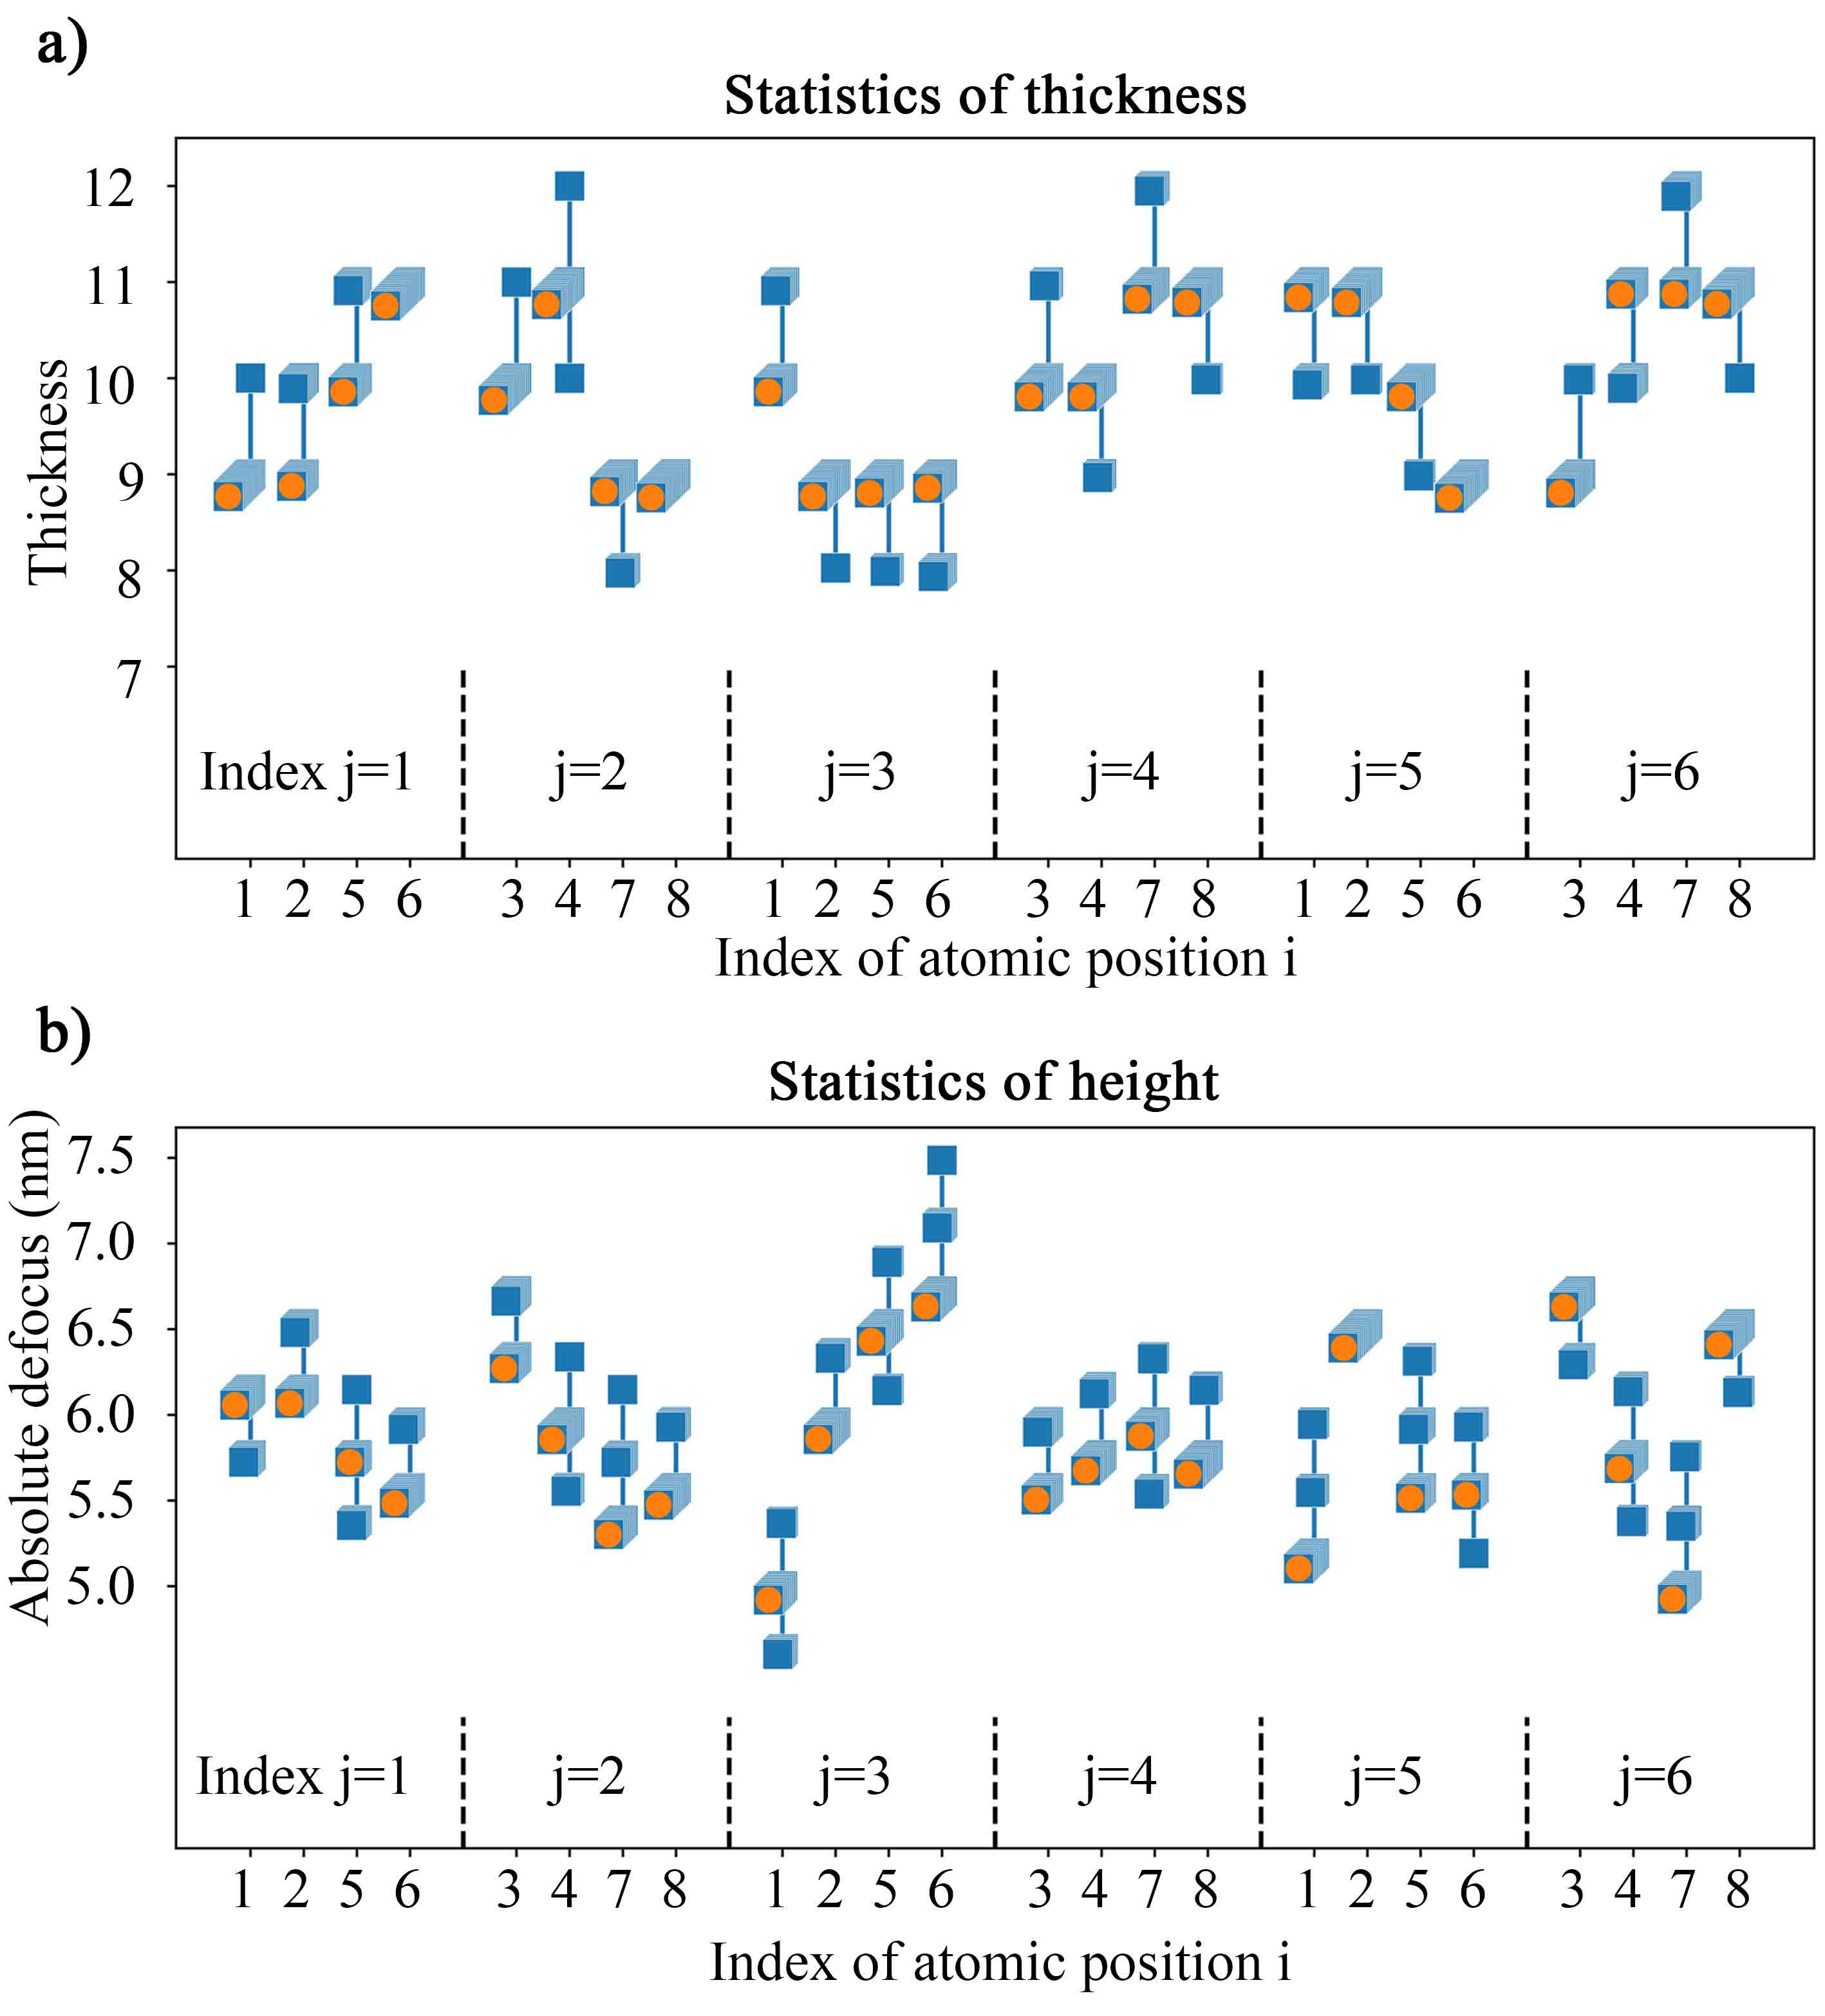
\includegraphics[width=0.85\textwidth]{../2.17/217}
	\caption{各原子柱的重构结果统计}\label{fig:217}
	\song\tuzhu{a) 原子柱厚度的统计结果;b) 原子柱高度的统计结果;橙色标记的是最终的平均结果,原子柱的索引与图 4.16c 一致}
\end{figure}




为了估算此次 Si[110] 样品的三维重构的置信度,图 4.19a-c 
展示了最终重构结果的高分辨模拟像(图 2.18a),感兴趣区域的实验图像(图 2.18b)以及两图像之间的误差(图 4.19c)。图 4.19c 的平均相对误差是 3.76\%,且从中可见,较大的误差发生在原子柱位置之间。进一步对比各原子柱位置的图像强度的结果如图 4.19d和 e 所示。其中,原子柱位置的图像强度是原子柱位置周围 $5\times 5$ 像素的平均强度值。模拟像中的原子柱位置的图像强度与实验像中原子柱位置的图像强度吻合度很高。原子柱位置的平均误差 $E_{column}$ 仅为 0.91\%。所以,根据公式(4.6)可得本次重构的置信度为 95.33\%。尽管许多不可控的因素将导致随机误差,但是非晶污染是主要的误差来源。在此基础上,根据图 4.13 中晶体厚度为 4 nm 时的误差曲线,估算此 Si[110] 样品表面覆盖的非晶层厚度为 0.5 nm。




\begin{figure}[H]
	\vspace{\baselineskip}
	\centering
	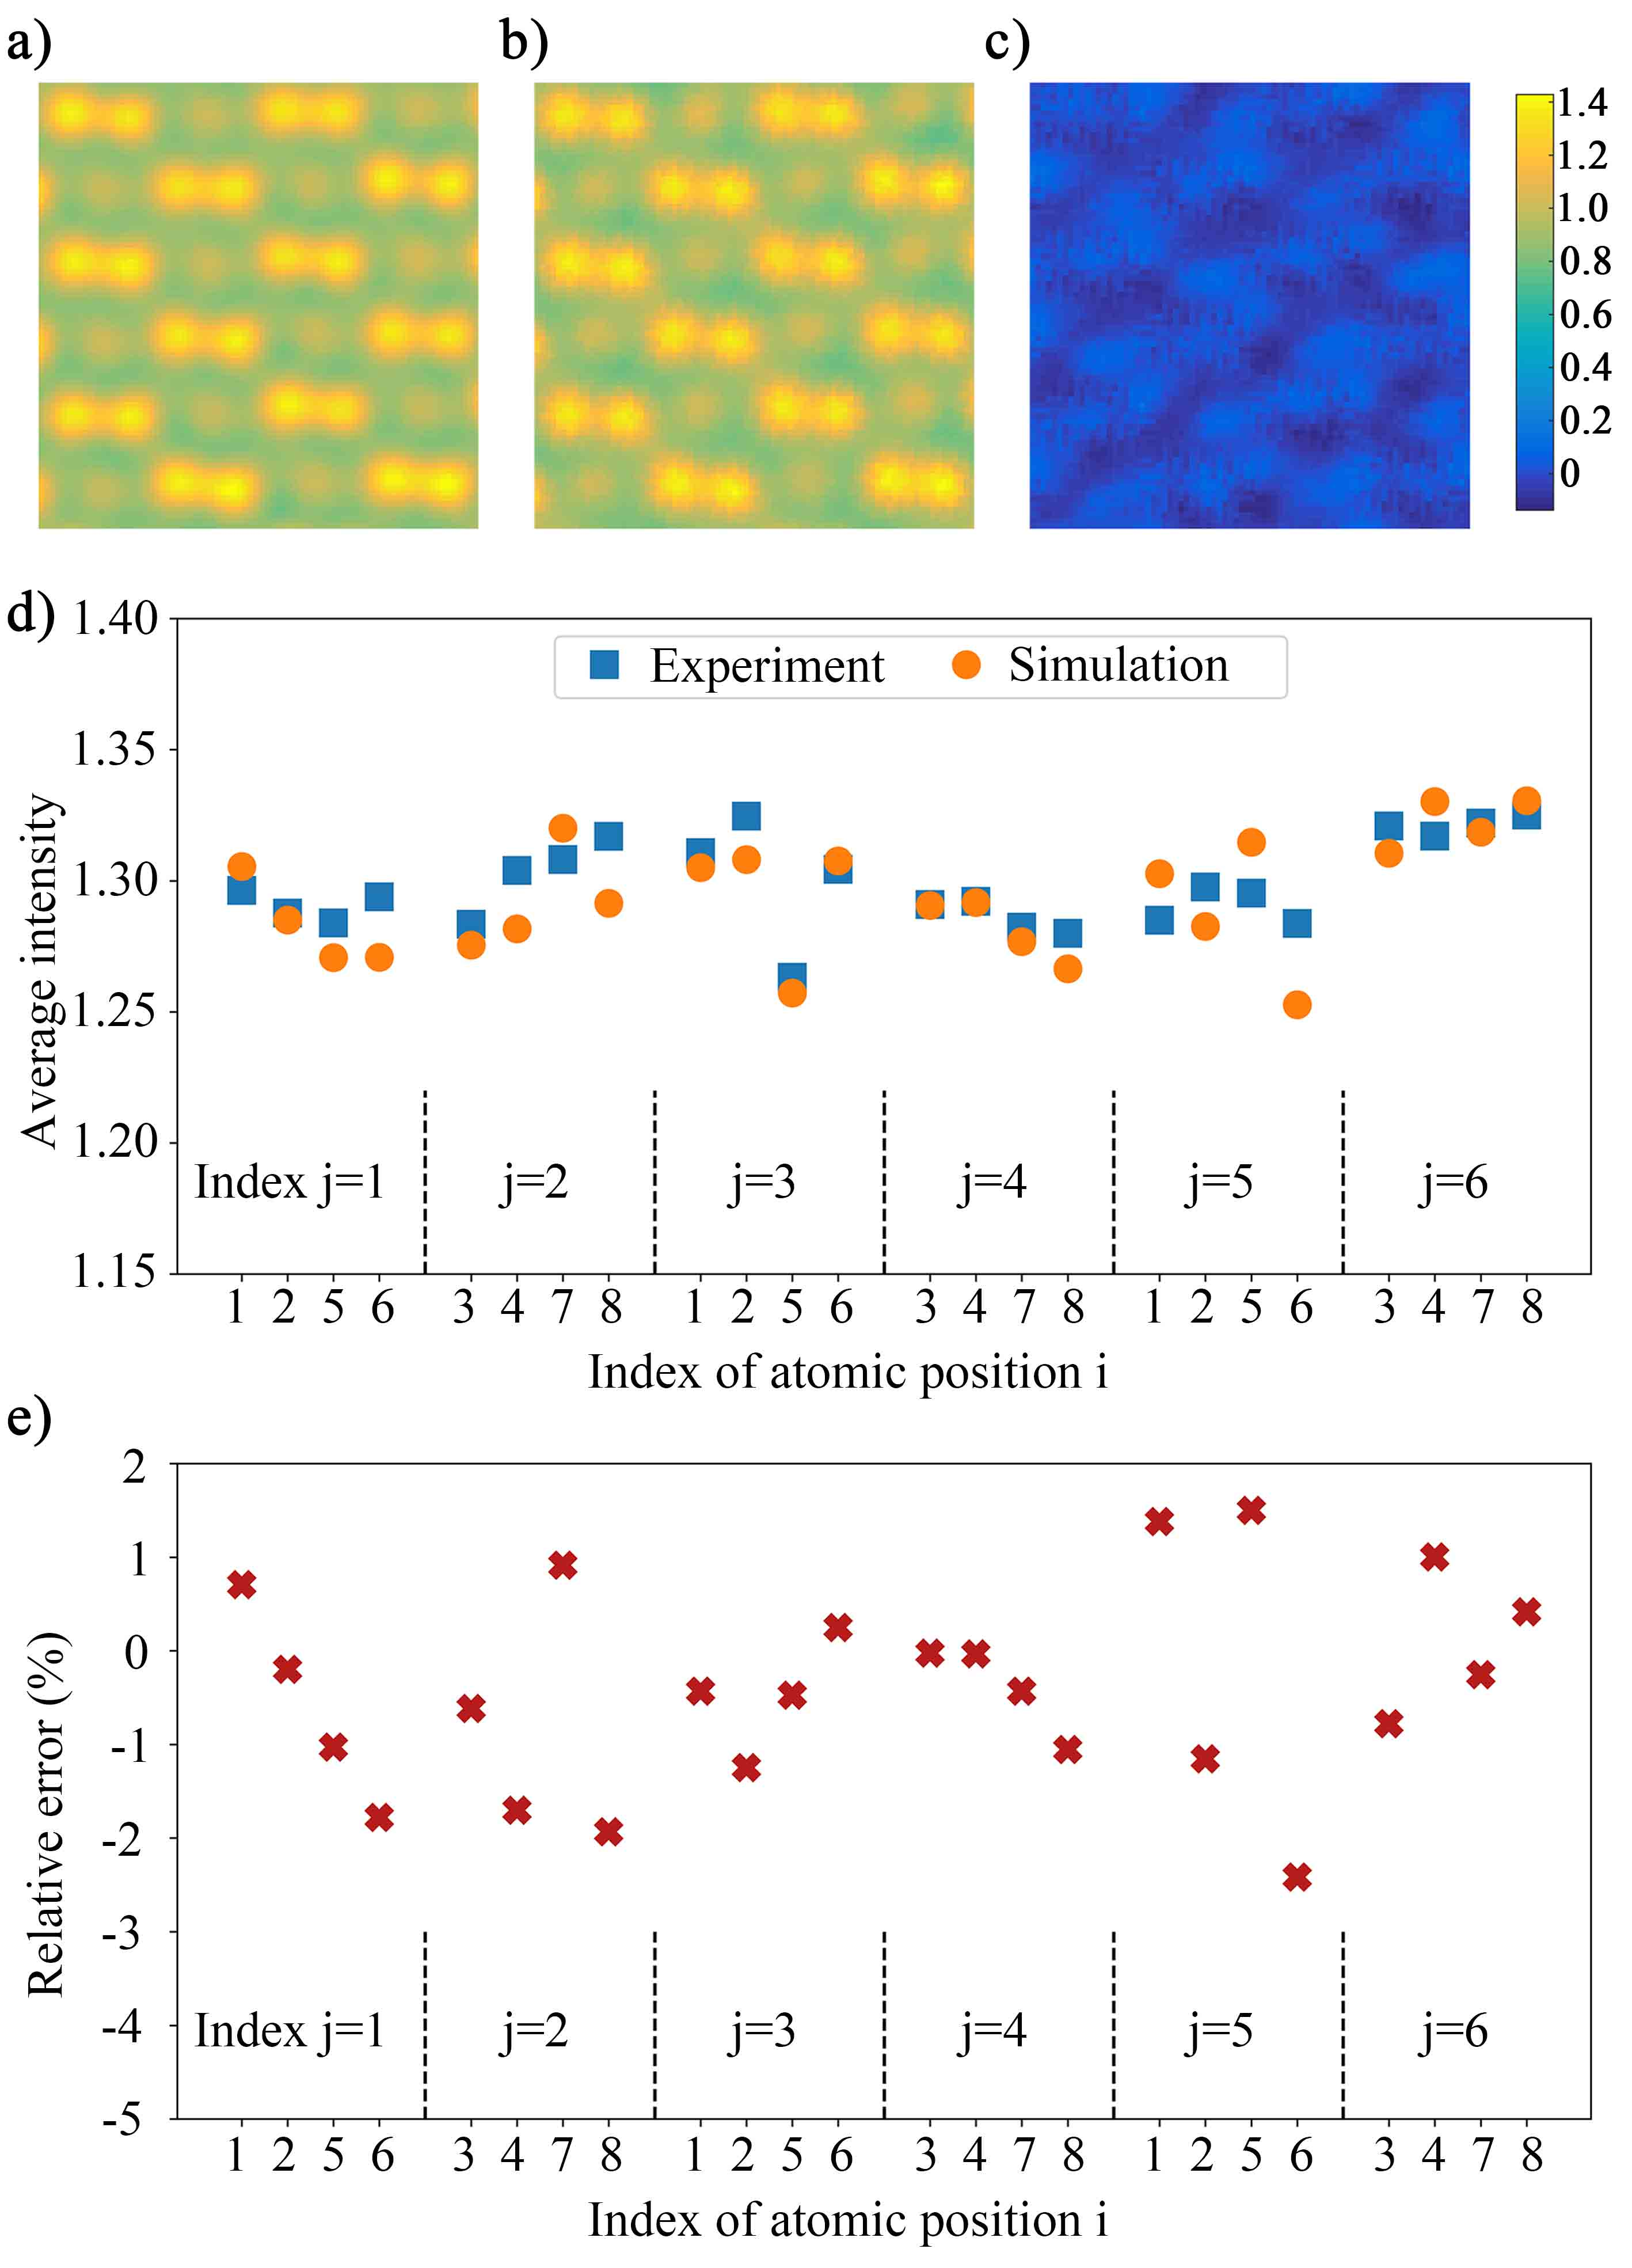
\includegraphics[width=0.85\textwidth]{../2.18/218}
	\caption{重构结果与实验图像的对比}\label{fig:218}
	\song\tuzhu{a) 平均重构结果的模拟像;b) 感兴趣区域的实验像;c) 图 a 和图 b 的差;d)原子柱位置的平均强度的散点图;e)重构的模拟像与实验像原子柱位置图像强度的相比误差;图d)和e)中原子柱的索引与图 4.17c 一致}
\end{figure}


最后,图 4.20a 和 b 展示了平均重构结果的表面原子形貌。图 4.20c 进一步统计了每一个原子柱的厚度(原子个数)和高度(欠焦量),并展示了它们在上表面以及下表面的分布情况。该样品的上下表面不是完全平滑的,而是在原子尺度上存在起伏。尽管不同原子柱的欠焦量不尽相同,但是样品的平均欠焦量为 +5.9 nm(图 4.20c 中下方的黑色虚线所示),这与 NCSI 技术下的最佳成像条件下的欠焦量(根据最佳相位衬度条件~\cite{Urban2009}计算,为 +5.88 nm)非常吻合。另外,样品的平均厚度为 3.84 nm(原子柱中包含 10 个原子)。因为 Si[110] 样品的表面 Si(110) 晶面不是低能量的晶面,所以重构所得样品的晶体表面参差不齐且有非晶覆盖的状态较为合理。而且,在目前的制样方法下,也很有可能产生这种不平整的样品表面状态。


\begin{figure}[H]
	\vspace{\baselineskip}
	\centering
	\includegraphics[width=0.8\textwidth]{../2.19/219}
	\caption{重构结果的三维形貌}\label{fig:219}
	\song\tuzhu{a,b) Si[110] 的 15 次重构的平均结果的上表面与下表面的示意图;c) 平均结果中每一个原子的空间绝对位置示意图,其中原子柱的索引与图 4.17c 一致}
\end{figure}






\section{本章小结}
本章提出了一种基于单张二维原子分辨率高分辨 TEM 照片重构材料三维原子形貌的方法。该方法利用了全局匹配算法定量对比实验像与模型像。研究中使用了模拟和实验的图像来测试该方法,从测试结果可以得出以下结论:

(1)为了在原子分辨率下从单张二维图像重构一般的晶体材料的表面,必须采取全局匹配算法和自洽性验证方案。这个方案采取若干次独立的三维重构的平均重构结果作为三维重构的最终结果。三维重构的分辨率可以定义为多次独立重构的重构结果之间的最大误差。同时,高于 90\% 的置信度也是保证三维重构可靠性的一个重要的指标。置信度可以通过定量对比重构结果的模拟像与原始实验图像来确定。


(2)三维重构的分辨率与置信度,与实验图像的质量密切相关。而实验图像的质量往往最容易受非晶污染的影响。如果实际样品表面覆盖的非晶厚度小于 1 nm,则三维重构的结果较可靠。

%% !Mode:: "TeX:UTF-8"

\chapter{绪~~论}
\section{引言}

透射电子显微镜(transmission electron microscopy,TEM)是现代材料科学研究中应用非常广泛的仪器。从1931年Ernst Ruska制造了世界上第一台电子显微镜(图1.1a)~\cite{das1932}至今,人类的显微镜分辨率以前所未有的速度提升(图1.1b)。球差矫正器的发明~\cite{dev1997}更是将透射电子显微镜(transmission electron microscopy,TEM)的分辨率提升至亚埃级别,使人类具备了观察原子的常规手段。同时,电子束在电镜中的成像过程、电子束与物质之间的相互作用、电子束转化为电信号的过程等的理论也日益发展成熟。这使得科研工作者能够正确理解TEM的成像原理,通过电子显微学的理论和分析方法,根据TEM的实验数据合理分析材料的结构与性质。

\begin{figure}[htbp]
	\vspace{\baselineskip}
	\centering
	\includegraphics[width=0.8\textwidth]{../1.1/11}
	\caption{世界上第一台电子显微镜与显微镜分辨率发展曲线}\label{fig:11}
	\song\wuhao{a) 世界上第一台电子显微镜;b) 显微镜分辨率发展曲线}
\end{figure}

材料的三维结构对其宏观性能具有非常重要的影响。比如铝合金中的析出相的形貌、尺寸以及分布决定其析出强化的效果;纳米颗粒的形貌和尺寸会影响其催化性能、分布状况等。揭示材料的三维结构、成分、分布等性质是材料科学研究中一个极其重要的问题。一般情况下,一张TEM像只能揭示材料在某一平面上的结构与性质,分析材料的三维信息需要进行更复杂的实验与理论分析。三维电子断层扫描

\section{下载安装}
HNUThesis~主页:~\url{http://hnuthesis.googlecode.com/}。除此之外,不再维护任何镜像。

\section{目录内容}
本~\LaTeX{}~模板的源文件即为研究生毕业设计论文中使用的模板,用户可以通过修改这些文件来编辑自己的毕业论文。
\begin{itemize}
\item{hnumain.tex}:主文件,包含封面部分和其他章节的引用信息。
\item{preface}: 包含本科毕业设计论文的封面和中英文摘要。
\item{body}: 包含本文正文中的所有章节。
\begin{itemize}
\item{intros.tex}: 包括本~\LaTeX{}~模板的介绍,编译方法和使用方法。
\item{figures.tex}: 包含论文中图片的插入和引用方法。
\item{tables.tex}: 包含论文中表格的插入和引用方法。
\item{equations.tex}: 包含论文中数学符号、公式的书写和排版方法。
\item{others.tex}: 包含论文中使用的罗列环境,定理环境等其他环境的排版方法。
\item{conclusion.tex}: 包含本文的总结。
\end{itemize}
\item{setup}:存放论文所使用的宏包和全文格式的定义。
\item{appendix}:存放作者的发表论文和参加科研情况说明以及致谢文件。
\item{references/reference.bib}:存放论文所引用的全部参考文献信息。
\item{clean.bat}:双击此文件,可以用来清理~hnumain.tex~在编译之后生成的所有附属文件,如后缀名为~.aux~,~.log~,~.bak~的文件。
\end{itemize}

需要说明的是,以上文件名并不是固定的,各位同学可以新建一个~tex~文件,例如~algorithm.tex,放在~body~目录下,并且在~hnumain.tex~中调用:
\begin{verbatim}
    \include{body/algorithm.tex}
\end{verbatim}
来引用之。当然你也可以重命名这些文件,只要~include~中的文件名是存在且合法,~\LaTeX~总能找到这些文件的。

在你写作某一章节的时候,你可能需要随时预览排版效果并~Debug,这时你可以在其他章节的\verb|\include|命令前加上一个\%,这代表注释掉本行,例如:
\begin{verbatim}
%%%%%%%%%%%%%%%%%%%%%%%%%%%%%%%%
           正文部分
%%%%%%%%%%%%%%%%%%%%%%%%%%%%%%%%
\mainmatter
% !Mode:: "TeX:UTF-8"

\chapter{绪~~论}
\section{引言}

透射电子显微镜(transmission electron microscopy,TEM)是现代材料科学研究中应用非常广泛的仪器。从1931年Ernst Ruska制造了世界上第一台电子显微镜(图1.1a)~\cite{das1932}至今,人类的显微镜分辨率以前所未有的速度提升(图1.1b)。球差矫正器的发明~\cite{dev1997}更是将透射电子显微镜(transmission electron microscopy,TEM)的分辨率提升至亚埃级别,使人类具备了观察原子的常规手段。同时,电子束在电镜中的成像过程、电子束与物质之间的相互作用、电子束转化为电信号的过程等的理论也日益发展成熟。这使得科研工作者能够正确理解TEM的成像原理,通过电子显微学的理论和分析方法,根据TEM的实验数据合理分析材料的结构与性质。

\begin{figure}[htbp]
	\vspace{\baselineskip}
	\centering
	\includegraphics[width=0.8\textwidth]{../1.1/11}
	\caption{世界上第一台电子显微镜与显微镜分辨率发展曲线}\label{fig:11}
	\song\wuhao{a) 世界上第一台电子显微镜;b) 显微镜分辨率发展曲线}
\end{figure}

材料的三维结构对其宏观性能具有非常重要的影响。比如铝合金中的析出相的形貌、尺寸以及分布决定其析出强化的效果;纳米颗粒的形貌和尺寸会影响其催化性能、分布状况等。揭示材料的三维结构、成分、分布等性质是材料科学研究中一个极其重要的问题。一般情况下,一张TEM像只能揭示材料在某一平面上的结构与性质,分析材料的三维信息需要进行更复杂的实验与理论分析。三维电子断层扫描

\section{下载安装}
HNUThesis~主页:~\url{http://hnuthesis.googlecode.com/}。除此之外,不再维护任何镜像。

\section{目录内容}
本~\LaTeX{}~模板的源文件即为研究生毕业设计论文中使用的模板,用户可以通过修改这些文件来编辑自己的毕业论文。
\begin{itemize}
\item{hnumain.tex}:主文件,包含封面部分和其他章节的引用信息。
\item{preface}: 包含本科毕业设计论文的封面和中英文摘要。
\item{body}: 包含本文正文中的所有章节。
\begin{itemize}
\item{intros.tex}: 包括本~\LaTeX{}~模板的介绍,编译方法和使用方法。
\item{figures.tex}: 包含论文中图片的插入和引用方法。
\item{tables.tex}: 包含论文中表格的插入和引用方法。
\item{equations.tex}: 包含论文中数学符号、公式的书写和排版方法。
\item{others.tex}: 包含论文中使用的罗列环境,定理环境等其他环境的排版方法。
\item{conclusion.tex}: 包含本文的总结。
\end{itemize}
\item{setup}:存放论文所使用的宏包和全文格式的定义。
\item{appendix}:存放作者的发表论文和参加科研情况说明以及致谢文件。
\item{references/reference.bib}:存放论文所引用的全部参考文献信息。
\item{clean.bat}:双击此文件,可以用来清理~hnumain.tex~在编译之后生成的所有附属文件,如后缀名为~.aux~,~.log~,~.bak~的文件。
\end{itemize}

需要说明的是,以上文件名并不是固定的,各位同学可以新建一个~tex~文件,例如~algorithm.tex,放在~body~目录下,并且在~hnumain.tex~中调用:
\begin{verbatim}
    \include{body/algorithm.tex}
\end{verbatim}
来引用之。当然你也可以重命名这些文件,只要~include~中的文件名是存在且合法,~\LaTeX~总能找到这些文件的。

在你写作某一章节的时候,你可能需要随时预览排版效果并~Debug,这时你可以在其他章节的\verb|\include|命令前加上一个\%,这代表注释掉本行,例如:
\begin{verbatim}
%%%%%%%%%%%%%%%%%%%%%%%%%%%%%%%%
           正文部分
%%%%%%%%%%%%%%%%%%%%%%%%%%%%%%%%
\mainmatter
% !Mode:: "TeX:UTF-8"

\chapter{绪~~论}
\section{引言}

透射电子显微镜(transmission electron microscopy,TEM)是现代材料科学研究中应用非常广泛的仪器。从1931年Ernst Ruska制造了世界上第一台电子显微镜(图1.1a)~\cite{das1932}至今,人类的显微镜分辨率以前所未有的速度提升(图1.1b)。球差矫正器的发明~\cite{dev1997}更是将透射电子显微镜(transmission electron microscopy,TEM)的分辨率提升至亚埃级别,使人类具备了观察原子的常规手段。同时,电子束在电镜中的成像过程、电子束与物质之间的相互作用、电子束转化为电信号的过程等的理论也日益发展成熟。这使得科研工作者能够正确理解TEM的成像原理,通过电子显微学的理论和分析方法,根据TEM的实验数据合理分析材料的结构与性质。

\begin{figure}[htbp]
	\vspace{\baselineskip}
	\centering
	\includegraphics[width=0.8\textwidth]{../1.1/11}
	\caption{世界上第一台电子显微镜与显微镜分辨率发展曲线}\label{fig:11}
	\song\wuhao{a) 世界上第一台电子显微镜;b) 显微镜分辨率发展曲线}
\end{figure}

材料的三维结构对其宏观性能具有非常重要的影响。比如铝合金中的析出相的形貌、尺寸以及分布决定其析出强化的效果;纳米颗粒的形貌和尺寸会影响其催化性能、分布状况等。揭示材料的三维结构、成分、分布等性质是材料科学研究中一个极其重要的问题。一般情况下,一张TEM像只能揭示材料在某一平面上的结构与性质,分析材料的三维信息需要进行更复杂的实验与理论分析。三维电子断层扫描

\section{下载安装}
HNUThesis~主页:~\url{http://hnuthesis.googlecode.com/}。除此之外,不再维护任何镜像。

\section{目录内容}
本~\LaTeX{}~模板的源文件即为研究生毕业设计论文中使用的模板,用户可以通过修改这些文件来编辑自己的毕业论文。
\begin{itemize}
\item{hnumain.tex}:主文件,包含封面部分和其他章节的引用信息。
\item{preface}: 包含本科毕业设计论文的封面和中英文摘要。
\item{body}: 包含本文正文中的所有章节。
\begin{itemize}
\item{intros.tex}: 包括本~\LaTeX{}~模板的介绍,编译方法和使用方法。
\item{figures.tex}: 包含论文中图片的插入和引用方法。
\item{tables.tex}: 包含论文中表格的插入和引用方法。
\item{equations.tex}: 包含论文中数学符号、公式的书写和排版方法。
\item{others.tex}: 包含论文中使用的罗列环境,定理环境等其他环境的排版方法。
\item{conclusion.tex}: 包含本文的总结。
\end{itemize}
\item{setup}:存放论文所使用的宏包和全文格式的定义。
\item{appendix}:存放作者的发表论文和参加科研情况说明以及致谢文件。
\item{references/reference.bib}:存放论文所引用的全部参考文献信息。
\item{clean.bat}:双击此文件,可以用来清理~hnumain.tex~在编译之后生成的所有附属文件,如后缀名为~.aux~,~.log~,~.bak~的文件。
\end{itemize}

需要说明的是,以上文件名并不是固定的,各位同学可以新建一个~tex~文件,例如~algorithm.tex,放在~body~目录下,并且在~hnumain.tex~中调用:
\begin{verbatim}
    \include{body/algorithm.tex}
\end{verbatim}
来引用之。当然你也可以重命名这些文件,只要~include~中的文件名是存在且合法,~\LaTeX~总能找到这些文件的。

在你写作某一章节的时候,你可能需要随时预览排版效果并~Debug,这时你可以在其他章节的\verb|\include|命令前加上一个\%,这代表注释掉本行,例如:
\begin{verbatim}
%%%%%%%%%%%%%%%%%%%%%%%%%%%%%%%%
           正文部分
%%%%%%%%%%%%%%%%%%%%%%%%%%%%%%%%
\mainmatter
\include{body/intros}
%%\include{body/figures}
%%\include{body/tables}
%%\include{body/equations}
%%\include{body/others}
%%\include{body/conclusion}
\end{verbatim}
那么,编译的时候就只编译未加~\%~的一章,在这个例子中,即本章~intros。

理论上,并不一定要把每章放在不同的文件中。但是这种自顶向下,分章节写作、编译的方法有利于提高效率,大大减少~Debug~过程中的编译时间,同时减小风险。

\section{参考文献生成方法}

\LaTeX~具有插入参考文献的能力。Google Scholar~网站上存在兼容~BibTeX~的参考文献信息,通过以下几个步骤,可以轻松完成参考文献的生成。
\begin{itemize}
  \item 在\href{http://scholar.google.com/}{谷歌学术搜索}中,
        点击\href{http://scholar.google.com/scholar_preferences?hl=en&as_sdt=0,5}{学术搜索设置}。
  \item 页面打开之后,在\textbf{文献管理软件}选项中选择\textbf{显示导入~BibTeX~的链接},单击保存设置,退出。
  \item 在谷歌学术搜索中检索到文献后,在文献条目区域单击导入~BibTeX~选项,页面中出现文献的引用信息。
  \item 将文献引用信息的内容复制之后,添加到~references~文件夹下的~reference.bib~中。
\end{itemize}

\section{编译注意事项}
\begin{enumerate}
  \item 由于模板使用~UTF-8~编码,所以源文件应该保存成~UTF-8~格式,否则可能出现中文字符无法识别的错误。
  本模板中每一个~.tex~文件的文件的开头已经加上一行:\\
    \verb|% !Mode:: "TeX:UTF-8"|\\
     这样可以确保~.tex~文件默认使用~UTF-8~的格式打开。读者如果删去此行,很有可能会导致中文字符显示乱码。
     在~WinEdt~编辑器中可以使用以下两种方式保存成~UTF-8~格式:
      \begin{enumerate}
        \item 先建立~.tex~文件,另存为~.tex~文件时,选择用~UTF-8~格式保存。
        \item
            在~WinEdt~编辑器中,选择\\
            \mbox{~Document$\to$Document Settings$\to$Document Mode $\to$TeX:UTF-8} 同时在~WinEdt~最下面的状态栏中,可以看到该文档是~TeX~格式还是~TeX:UTF-8~格式。
            当文档为~TeX:UTF-8~格式时,状态栏一般显示:
            \makebox[\textwidth][l]{Wrap | Indent | INS | LINE |Spell | TeX:UTF-8 | -src~ 等。}
      \end{enumerate}
  \item 如果在pdf书签中,中文显示乱码的话,则注意以下说明:
    \begin{verbatim}
        \usepackage{CJKutf8}
        % 1. 如果使用CJKutf8
        %    Hyperref中应使用unicode参数
        % 2. 如果使用CJK
        %    Hyperref则使用CJKbookmarks参数
        %    可惜得到的PDF书签是乱码,建议弃用
        % 3. Unicode选项和CJKbookmarks不能同时使用
        \usepackage[
        %CJKbookmarks=true,
        unicode=true
        ]{hyperref}
     \end{verbatim}
 \item 建议采用以下两种编译方式:
  \begin{enumerate}
     \item latex + bibtex + latex + latex + dvi2pdf. 在这种编译情况下,对应的~hnumain.tex~文件的第一行是\verb|\def\usewhat{dvipdfmx}|~(缺省设置)。 此时,所有图片文件应该保存为~.eps~格式,如~figures~文件夹里~.eps~图片。
          如果您选择在命令行中操作,可以在编译的时候依次输入~latex hnumain, bibtex hnumain, latex hnumain, latex hnumain~和~dvipdfmx hnumain, 编译完成之后,需要手动打开~pdf~文件。
     \item pdflatex + pdflatex. 在这种编译情况下,对应的~hnumain.tex~文件的第一行应该改为\verb|\def\usewhat{pdflatex}|~。 此时, 编译不支持~.eps~图片格式,此时需要在命令行下使用~epstopdf~指令将~figures~文件夹下 的~.eps~文件转化成~.pdf~文件格式,命令行中操作格式为~epstopdf a.eps~。
          在命令行编译的时候,依次输入~pdflatex hnumain~和~pdflatex hnumain, 编译完成之后,需要手动打开~pdf~文件。
  \end{enumerate}
\end{enumerate}

\section{系统要求}
    CTEX 2.8, MiKTeX 2.8, TeX Live 2009~或以上版本。使用推荐的~WinEdt 6.0~编辑器,可以完成文件的编辑和编译工作。

\section{\TeX~简介}

以下内容是~milksea@bbs.ctex.org~撰写的关于~\TeX~的简单介绍,略有改动。
注意这不是一个入门教程,不讲~\TeX~系统的配置安装,也不讲具体的~\LaTeX~代码。
这里仅仅试图以一些只言片语来解释:
进入这个门槛之前新手应该知道的注意事项,以及遇到问题以后该去如何解决问题。

\subsection{什么是 \TeX/\LaTeX,我是否应该选择它~?}

\TeX~是最早由高德纳(Donald Knuth)教授创建的一门标记式宏语言,
用来排版科技文章,尤其擅长处理复杂的数学公式。\TeX~同时也是处理这一语言的排版软件。
\LaTeX~是 Leslie Lamport 在~\TeX~基础上按内容/格式分离和模块化等思想建立的一集~\TeX~上的格式。

\TeX~本身的领域是专业排版领域
但现在~TeX/LaTeX~也被广泛用于生成电子文档甚至幻灯片等,~\TeX~语言的数学部分
偶尔也在其他一些地方使用。但注意~\TeX~并不适用于文书处理(Microsoft Office 的领域,以前和现在都不是)。

选择使用~\TeX/\LaTeX~的理由包括:
\begin{itemize}
\item 免费软件;
\item 专业的排版效果;
\item 是事实上的专业数学排版标准;
\item 广泛的西文期刊接收甚或只接收 LaTeX 格式的投稿;
\item[] ……
\end{itemize}
不选择使用~\TeX/\LaTeX~的理由包括:
\begin{itemize}
\item 需要相当精力学习;
\item 图文混合排版能力不够强;
\item 仅在数学、物理、计算机等领域流行;
\item 中文期刊的支持较差;
\item[] ……
\end{itemize}

请尽量清醒看待网上经常见到的关于~\TeX~与其他软件的优劣比较和口水战。在选择使用或离开之前,请先考虑
\TeX~的应用领域,想想它是否适合你的需要。


\subsection{我该用什么编辑器~?}

编辑器功能有简有繁,特色不一,从简单的纯文本编辑器到繁复的 Emacs,因人而易。基本功能有语法高亮、方便编译预览就很好了,扩充功能和定制有无限的可能。初学者可以使用功能简单、使用方便的专用编辑器,如 ~TeXWorks、Kile、WinEdt~等,或者类似所见即所得功能的~LyX;熟悉的人可以使用定制性更强的~Notepad++、SciTE、Vim、Emacs ~等。这方面的介绍很多,一开始不妨多试几种,找到最适合自己的才是最好的。

另外提醒一句,编辑器只是工作的助手,不必把它看得太重。

\subsection{我应该看什么~\LaTeX~读物~?}

这不是一个容易回答的问题,因为有许多选择,也同样有许多不合适的选择。
这里只是选出一个比较好的答案。更多更详细的介绍可以在版面和网上寻找(注意时效)。

近两年~\TeX~的中文处理发展很快,目前没有哪本书在中文处理方面给出一个最新进展的合适综述,
因而下面的介绍也不主要考虑中文处理。

\begin{enumerate}

\item 我能阅读英文。
\begin{enumerate}
\item 迅速入门:ltxprimer.pdf (LaTeX Tutorials: A Primer, India TUG)
\item 系统学习:A Guide to LaTeX, 4th Edition, Addison-Wesley
               有机械工业出版社的影印版(《\LaTeX{}~实用教程》)
\item 深入学习:要读许多书和文档,TeXbook 是必读的
\item 细节学习:去读你使用的每一个宏包的说明文档
\item 专题学习:阅读讲数学公式、图形、表格、字体等的专题文档
\end{enumerate}

\item 我更愿意阅读中文。
\begin{enumerate}
\item 迅速入门:lnotes.pdf (LaTeX Notes, 1.20, Alpha Huang)
\item 系统学习:《\LaTeXe{}~科技排版指南》,邓建松(电子版)
      如果不好找,可以阅读《\LaTeXe~入门与提高》第二版,陈志杰等,或者 《\LaTeXe~完全学习手册》,胡伟
\item 深入学习:~TeXbook0.pdf~(特可爱原本,TeXbook 的中译,xianxian)
\item 具体问题释疑:~CTeX-FAQ.pdf~,\\
        吴凌云,~\url{http://www.ctex.org/CTeXFAQ}~
\end{enumerate}
\end{enumerate}

遇见问题和解决问题的过程可以快速提高自己的技能,建议此时:
\begin{itemize}
  \item 利用~Google~搜索。
  \item 清楚,扼要地提出你的问题。
\end{itemize}

\subsection{什么知识会过时~?什么不会~?}

\TeX~是排版语言,也是广泛使用的软件,并且不断在发展中;
因此,总有一些东西会很快过时。作为学习~\TeX~的人,
免不了要看各种各样的书籍、电子文档和网络论坛上的只言片语,
因此了解什么知识会迅速过时,什么知识不会是十分重要的。

最稳定的是关于~Primitive \TeX~和~Plain \TeX~的知识,也就是 Knuth
在他的《The TeXbook》中介绍的内容。因为~\TeX~
系统开发的初衷就是稳定性,要求今天的文档到很久以后仍可以得到完全相同的结果,
因此 Knuth 限定了他的~\TeX~语言和相关实现的命令、语法。这些内容许多年来就没有多少变化,
在未来的一些年里也不会有什么变化。
Primitive \TeX~和 Plain \TeX~的知识主要包括 \TeX~排版的基本算法和原理,
盒子的原理,底层的 \TeX~命令等。其中技巧性的东西大多在宏包设计中,
初学者一般不会接触到很多;而基本原理则是常常被提到的,
譬如,~\TeX~把一切排版内容作为盒子(box)处理。

相对稳定的是关于基本~\LaTeXe~
的知识,也包括围绕~\LaTeXe~的一些核心宏包的知识。~\LaTeXe~
是自~1993~年以来的一个稳定的~\LaTeX~版本,直到最近的一次修订
(2005 年)都没有大的变动。
\LaTeX~的下一个计划中的版本~\LaTeX 3~遥遥无期,在可预见的将来,~\LaTeXe~不会过时。
\LaTeXe~的知识是目前大部分~\LaTeX~书籍的主体内容。关于~\LaTeX~的标准文档类
~(article、report、book、letter、slide~等),关于基本数学公式的输入,
文档的章节层次,表格和矩阵,图表浮动体,LR 盒子与段落盒子……
这些~\LaTeX~的核心内容都是最常用的,相对稳定的。
与~\LaTeXe~相匹配的核心宏包,
如~graphics(x)、ifthen、fontenc、doc~等,也同样是相对稳定的。
还有一些被非常广泛应用的宏包,如~amsmath~系列,也可以看作是相对稳定的。

简单地说,关于基本~\TeX/\LaTeX~的语言,都是比较稳定的。与之对应,实现或者支持~\TeX/\LaTeX~语言的软件,
包括在~\TeX/\LaTeX~基础上建立的新的宏,都不大稳定。

容易过时的是关于第三方~\LaTeX~宏包的知识、第三方~\TeX~工具的知识,以及新兴~\TeX~相关软件的知识等。
~\TeX~和~\LaTeX~语言是追求稳定的;但无论是宏包还是工具,作为不断更新软件,它们是不稳定的。
容易过时的技术很多,而且现在广泛地出现在几乎所有~\LaTeX~文档之中,因此需要特别引起注意:
宏包的过时的原因可
网络论坛上的只言片语的因此了解什么知识会迅速过时的什么知识不会是十分重
网络论坛上的只言片语的因此了解什么知识会迅速过时的什么知识不会是十分重
网络论坛上的只言片语的因此了解什么知识会迅速过时的什么知识不会是十分重
网络论坛上的只言片语的因此了解什么知识会迅速过时的什么知识不会是十分重
网络论坛上的只言片语的因此了解什么知识会迅速过时的什么知识不会是十分重
网络论坛上的只言片语的因此了解什么知识会迅速过时的什么知识不会是十分重
网络论坛上的只言片语的因此了解什么知识会迅速过时的什么知识不会是十分重
网络论坛上的只言片语的因此了解什么知识会迅速过时的什么知识不会是十分重
网络论坛上的只言片语的因此了解什么知识会迅速过时的什么知识不会是十分重
网络论坛上的只言片语的因此了解什么知识会迅速过时的什么知识不会是十分重
网络论坛上的只言片语的因此了解什么知识会迅速过时的什么知识不会是十分重
网络论坛上的只言片语的因此了解什么知识会迅速过时的什么知识不会是十分重
网络论坛上的只言片语的因此了解什么知识会迅速过时的什么知识不会是十分重
网络论坛上的只言片语的因此了解什么知识会迅速过时的什么知识不会是十分重
网络论坛上的只言片语的因此了解什么知识会迅速过时的什么知识不会是十分重
网络论坛上的只言片语的因此了解什么知识会迅速过时的什么知识不会是十分重
网络论坛上的只言片语的因此了解什么知识会迅速过时的什么知识不会是十分重
网络论坛上的只言片语的因此了解什么知识会迅速过时的什么知识不会是十分重
网络论坛上的只言片语的因此了解什么知识会迅速过时的什么知识不会是十分重
网络论坛上的只言片语的因此了解什么知识会迅速过时的什么知识不会是十分重
网络论坛上的只言片语的因此了解什么知识会迅速过时的什么知识不会是十分重
网络论坛上的只言片语的因此了解什么知识会迅速过时的什么知识不会是十分重
网络论坛上的只言片语的因此了解什么知识会迅速过时的什么知识不会是十分重
网络论坛上的只言片语的因此了解什么知识会迅速过时的什么知识不会是十分重
网络论坛上的只言片语的因此了解什么知识会迅速过时的什么知识不会是十分重
网络论坛上的只言片语的因此了解什么知识会迅速过时的什么知识不会是十分重
网络论坛上的只言片语的因此了解什么知识会迅速过时的什么知识不会是十分重
网络论坛上的只言片语的因此了解什么知识会迅速过时的什么知识不会是十分重
网络论坛上的只言片语的因此了解什么知识会迅速过时的什么知识不会是十分重
网络论坛上的只言片语的因此了解什么知识会迅速过时的什么知识不会是十分重
网络论坛上的只言片语的因此了解什么知识会迅速过时的什么知识不会是十分重
网络论坛上的只言片语的因此了解什么知识会迅速过时的什么知识不会是十分重
网络论坛上的只言片语的因此了解什么知识会迅速过时的什么知识不会是十分重
网络论坛上的只言片语的因此了解什么知识会迅速过时的什么知识不会是十分重
网络论坛上的只言片语的因此了解什么知识会迅速过时的什么知识不会是十分重
网络论坛上的只言片语的因此了解什么知识会迅速过时的什么知识不会是十分重
网络论坛上的只言片语的因此了解什么知识会迅速过时的什么知识不会是十分重
能是宏包本身的升级换代带来了新功能或不兼容,
也可能是同一功能的更新更好的宏包代替了旧的宏包。前者的典型例子比如绘图宏包~PGF/TikZ~,
现在的~2.00~版功能十分强大,和旧的~1.1x~版相差很大,和更旧的~0.x~版本则几乎完全不同;后
者的典型例子比如~caption~宏包先是被更新的~caption2~宏包代替,后来~caption~宏包更新又使得
caption2 宏包完全过时。——安装更新的发行版可以避免使用过旧的宏包;
认真阅读宏包自带的文档而不是搜索得到的陈旧片断可以避免采用过时的代码。

工具过时的主要原因也是升级换代和被其他工具替换。前者的典型例子是编辑器
WinEdt~在~5.5~以后的版本支持~UTF-8~编码,而旧版本不支持;
后者的典型例子是中文字体安装工具从~GBKFonts~到~xGBKFonts~到~FontsGen~不断被取代。
图形插入是一个在~\TeX~实现、宏包与外围工具方面都更新很快的东西。
在过去,最常用的输出格式是~PS(PostScript)~格式,因此插入的图像以~EPS~为主流。
使用~Dvips~为主要输出工具,外围工具有~GhostScript、bmeps~等等,相关宏包有~graphics~等,
相关文档如《\LaTeXe{}~ 插图指南》。

但凡提及“~\LaTeX~只支持~EPS~图形”的,就是这个过时的时代的产物。事实上~\TeX/\LaTeX~
并不限定任何图形格式,只不过是当时的输出格式(PS)和工具(Dvips)对~EPS~情有独钟而已。
后来 PDF 格式成为主流。~pdf\TeX、DVIPDFM、DVIPDFMx、XeTeX~工具则主要支持~PDF、PNG、JPG~格式的图形,
涉及一系列工具如~ImageMagick、ebb~等。

值得特别提出注意的就是,中文处理也一起是更新迅速、容易过时的部分。
而且因为中文处理一直没有一个“官方”的“标准”做法,软件、工具、
文档以及网上纷繁的笔记也就显得相当混乱。从八十年代开始的~CCT~系统、
天元系统,到后来的~CJK~方式,到近来的~XeTeX~和~LuaTeX~ 方式,
中文处理的原理、软件、宏包、配置方式等都在不断变化中。

%\section{后期工作}
%下表记录了~HNUThesis~计划中未来应该逐步实现的功能和特性:
%\begin{enumerate}
%  \item 编写更为详细的~HNUThesis~的使用手册和~FAQ~用户指南
%  \item 加入对课程结课论文的支持
%  \item 加入对天津大学学生经常参加的各种限时完成重大赛事的论文模板的支持,如全国研究生数学建模竞赛,以节省排版时间
%  \item 加入对~pdf~书签中章节中文编号的支持,如: 第1章 XXX
%  \item 加入对附录~A~等格式的支持
%  \item Linux~平台迁移和测试
%\end{enumerate}

\section{免责声明}

本模板依据《湖南大学关于博士、硕士学位论文统一格式的规定》和《湖南大学硕士论文模版》编写,适用于所有博士生的学位论文编写。然而,作者不保证本模板完全符合学校要求,也不对由此带来的风险和损失承担任何责任。

%%% !Mode:: "TeX:UTF-8"

\chapter{图片的插入方法}

\section{研究生毕业论文的插图规范}

图应有自明性。插图应与文字紧密配合,文图相符,内容正确。选图要力求精练,插图、照片应完整清晰。图中文字和数字等字号用宋体五号字。

机械工程图:采用第一角投影法,严格按照~GB4457---GB131-83《机械制图》标准规定。

数据流程图、程序流程图、系统流程图等按~GB1526-89~标准规定。

电气图:图形符号、文字符号等应符合有关标准的规定。

流程图:必须采用结构化程序并正确运用流程框图。

对无规定符号的图形应采用该行业的常用画法。

坐标图的坐标线均用细实线,粗细不得超过图中曲线,有数字标注的坐标图,必须注明坐标单位。

照片图要求主题和主要显示部分的轮廓鲜明,便于制版。如用放大或缩小的复制品,必须清晰,反差适中。照片上应有表示目的物尺寸的标度。

引用文献图表必须标注出处。

\subsection{图题及图中说明}
每个图均应有图题(由图序和图名组成),图名在图序之后空两格排写。图序按章编排,如第~1~章第一个插图的图号为“图~1-1”等。
图题置于图下,要求中文用宋体五号字,位置居中。有图注或其它说明时应置于图题之上。引用图应注明出处,在图题右上角加引用文献号。
图中若有分图时,分图题置于分图之下或图题之下,分图号用~a)、b)等表示。

图中各部分说明应采用中文(引用的外文图除外)或数字项号,各项文字说明置于图题之上(有分图题者,置于分图题之上)。

\subsubsection{adad}
的还很大搜集

\subsection{插图编排}
插图之前,文中必须有关于本插图的提示,如“见图~1-1”、“如图~1-1~所示”等。插图与其图题为一个整体,不得拆开排写于两页。
插图处的该页空白不够排写该图整体时,则可将其后文字部分提前排写,将图移到次页。

\section{\LaTeX~中推荐使用的图片格式}
在~\LaTeX~中应用最多的图片格式是~EPS(Encapsulated PostScript)格式,它是一种专用的打印机描述语言,常用于印刷或打印输出。
EPS~格式图片可通过多种方式生成,这里介绍一款功能强大的免费图片处理软件———\href{http://www.imagemagick.org/}{ImageMagick},
此软件可将其它格式图片转换为~EPS~格式图片,同时还可以锐化图片,使图片的局部清晰一些。

此软件对图片的格式转换操作都是在命令提示符(cmd.exe)中实现的,可以通过“开始$\to$运行$\to$输入~cmd$\to$回车”或
“开始$\to$程序$\to$附件$\to$命令提示符”找到它。在命令提示符下,首先采用“盘符命令”或“cd~命令”将当前目录改为待处理图片所在的目录,
在此目录下就可通过~convert~命令将图片转换为~EPS~格式,其命令的语法格式为

\indent\verb|convert [可选参数] 原文件名.原扩展名 新文件名.eps|.

若~convert~命令中无可选参数,则将原来的图片格式直接转换为~EPS~格式,对图片不进行任何处理,这也是最常用的方法。
也可以选用可选参数,可选参数有很多选择,但最常用的有如下两个:

\verb|-sharpen radius{xsigma}|———此参数用来锐化图片,一般用在图片像素不高,需要提高图片清晰度的情况下。其中~radius~只能为整数,
它用来确定转换命令采取哪一种锐化算法,我们可以只取~radius~为~0;sigma~为所采取算法的锐化度,它的取值为~$0.1 - 3$~之间的任意一个浮点数,
数值越大,锐化程度也越大,通常取为~$0.1 - 3$~之间;x~在参数中为分隔符。

\verb|-resize geometry|———此参数用来改变图片的大小,若图片的存储空间过大,可通过此命令缩小图片尺寸,但同时也将导致图片像素降低,
其具体用法请参见\href{http://www.imagemagick.org/script/command-line-options.php#resize}{-resize geometry~的官方说明}。

除此之外,一些文字处理软件和科学计算软件也支持生成~EPS~格式的文件,请使用“另存为”功能查看某款软件是否能够将图片以~EPS~格式的形式保存。

\section{单张图片的插入方法}
单张图片独自占一行的插入形式如图~\ref{fig:word}~所示。
\begin{figure}[htbp]
\centering
\includegraphics[width=0.8\textwidth]{aaa}
\caption{树状结构}\label{fig:word}
\vspace{\baselineskip}
\end{figure}


其插入图片的代码及其说明如下。
\vspace{1em}\noindent\hrule
\begin{verbatim}
\begin{figure}[htbp]
\centering
\includegraphics[width=0.4\textwidth]{文件名(.eps)}
\caption{标题}\label{标签名(通常为 fig:labelname)}
\vspace{\baselineskip} %表示图与正文空一行
\end{figure}
\end{verbatim}

\noindent\hrule

\begin{verbatim}
figure环境的可选参数[htbp]表示浮动图形所放置的位置,h (here)表示当前位置,t (top)表示页芯顶部,b (bottom)表示页芯底部,p (page)表示单独一页。在Word等软件中,图片通常插入到当前位置,如果当前页的剩余空间不够,图片将被移动到下一页,当前页就会出现很大的空白,其人工调整工作非常不便。由LaTeX提供的浮动图片功能,总是会按h->t->b->p的次序处理选项中的字母,自动调整图片的位置,大大减轻了工作量。
\centering命令将后续内容转换成每行皆居中的格式。
"\includegraphics"的可选参数用来设置图片插入文中的水平宽度,一般表示为正文宽度(\textwidth)的倍数。
\caption命令可选参数“标签名”为英文形式,一般不以图片或表格的数字顺序作为标签,而应包含一定的图片或表格信息,以便于文中引用(若图片、表格、公式、章节和参考文献等在文中出现的先后顺序发生了变化,其标注序号及其文中引用序号也会跟着发生变化,这一点是Word等软件所不能做到的)。另外,图题或表题并不会因为分页而与图片或表格体分置于两页,章节等各级标题也不会置于某页的最底部,LaTeX系统会自动调整它们在正文中的位置,这也是Word等软件所无法匹敌的。
\vspace将产生一定高度的竖直空白,必选参数为负值表示将后续文字位置向上提升,参数值可自行调整。em为长度单位,相当于大写字母M的宽度。\vspace{\baselineskip} 表示图与正文空一行。
引用方法:“见图~\ref{fig:figname}”、“如图~\ref{fig:figname}~所示”等。
\end{verbatim}

\noindent\hrule\vspace{1em}

若需要将~2~张及以上的图片并排插入到一行中,则需要采用\verb|minipage|环境,如图~\ref{fig:dd}~和图~\ref{fig:ds}~所示。
\begin{figure}[htbp]
\centering
\begin{minipage}{0.4\textwidth}
\centering
\includegraphics[width=\textwidth]{dataDimensions}
\caption{数据维数的变化}\label{fig:dd}
\end{minipage}
\begin{minipage}{0.4\textwidth}
\centering
\includegraphics[width=\textwidth]{dataSize}
\caption{数据规模的变化}\label{fig:ds}
\end{minipage}
\vspace{\baselineskip}
\end{figure}

其代码如下所示。
\vspace{1em}\noindent\hrule
\begin{verbatim}
\begin{figure}[htbp]
\centering
\begin{minipage}{0.4\textwidth}
\centering
\includegraphics[width=\textwidth]{文件名}
\caption{标题}\label{fig:f1}
\end{minipage}
\begin{minipage}{0.4\textwidth}
\centering
\includegraphics[width=\textwidth]{文件名}
\caption{标题}\label{fig:f2}
\end{minipage}\vspace{\baselineskip}
\end{figure}
\end{verbatim}

\noindent\hrule

\begin{verbatim}
minipage环境的必选参数用来设置小页的宽度,若需要在一行中插入n个等宽图片,则每个小页的宽度应略小于(1/n)\textwidth。
\end{verbatim}

\noindent\hrule

\section{具有子图的图片插入方法}

图中若含有子图时,需要调用~subfigure~宏包, 如图~\ref{fig:subfig}~所示。
\begin{figure}[htbp]
  \centering
  \subfigure[Data Dimensions]{\label{fig:subfig:datadim}
                \includegraphics[width=0.4\textwidth]{dataDimensions}}
  \subfigure[Data Size]{\label{fig:subfig:datasize}
                \includegraphics[width=0.4\textwidth]{dataSize}}
  \caption{Scalability of data}\label{fig:subfig}
\vspace{\baselineskip}
\end{figure}

其代码及其说明如下。
\vspace{1em}\noindent\hrule

\begin{verbatim}
\begin{figure}[htbp]
  \centering
  \subfigure[第1个子图标题]{
            \label{第1个子图标签(通常为 fig:subfig1:subsubfig1)}
            \includegraphics[width=0.4\textwidth]{文件名}}
  \subfigure[第2个子图标题]{
            \label{第2个子图标签(通常为 fig:subfig1:subsubfig2)}
            \includegraphics[width=0.4\textwidth]{文件名}}
  \caption{总标题}\label{总标签(通常为 fig:subfig1)}
\vspace{\baselineskip}
\end{figure}
\end{verbatim}

\noindent\hrule

\begin{verbatim}
子图的标签实际上可以随意设定,只要不重复就行。但为了更好的可读性,我们建议fig:subfig:subsubfig格式命名,这样我们从标签名就可以知道这是一个子图引用。
引用方法:总图的引用方法同本章第1节,子图的引用方法用\ref{fig:subfig:subsubfig}来代替。
\end{verbatim}

\noindent\hrule\vspace{1em}

子图的引用示例:如图~\ref{fig:subfig:datadim}~和图~\ref{fig:subfig:datasize}~所示。

若想获得插图方法的更多信息,参见网络上的~\href{ftp://ftp.tex.ac.uk/tex-archive/info/epslatex.pdf}{Using Imported Graphics in \LaTeX and pdf\LaTeX}~文档。 
%%% !Mode:: "TeX:UTF-8"

\chapter{表格的绘制方法}
\section{研究生毕业设计论文的绘表规范}

表应有自明性。表格不加左、右边线。表的编排建议采用国际通行的三线表。表内中文书写使用宋体五号字。

每个表格之上均应有表题(由表序和表名组成)。表序一般按章编排,如第~1~章第一个插表的序号为“表~1-1”等。表序与表名之间空两格,
表名使用中文五号字,居中。表名中不允许使用标点符号,表名后不加标点。
表头设计应简单明了,尽量不用斜线。表头中可采用化学,物理量等专业符号。

全表如用同一单位,则将单位符号移至表头右上角,加圆括号\cite{djy}。
表中数据应准确无误,书写清楚。数字空缺的格内加横线“-”(占~2~个数字宽度)。表内文字或数字上、下或左、右相同时,
采用通栏处理方式,不允许用“〃”、“同上”之类的写法。

表内文字使用宋体五号字,垂直居中书写,起行空一格、转行顶格、句末不加标点。
如某个表需要转页接排,在随后的各页上应重复表的编号。编号后加“(续表)”,表题可省略。续表应重复表头。
表格绘制完成之后,与正文空一行。

\section{普通表格的绘制方法}

表格应具有三线表格式,因此需要调用~booktabs~宏包,其标准格式如表~\ref{tab:table1}~所示。
\begin{table}[htbp]
\caption{符合本科生毕业论文绘图规范的表格}\label{tab:table1}
\vspace{0.5em}\centering\wuhao
\begin{tabular}{ccccc}
\toprule[1.5pt]
$D$(in) & $P_u$(lbs) & $u_u$(in) & $\beta$ & $G_f$(psi.in)\\
\midrule[1pt]
 5 & 269.8 & 0.000674 & 1.79 & 0.04089\\
10 & 421.0 & 0.001035 & 3.59 & 0.04089\\
20 & 640.2 & 0.001565 & 7.18 & 0.04089\\
 5 & 269.8 & 0.000674 & 1.79 & 0.04089\\
10 & 421.0 & 0.001035 & 3.59 & 0.04089\\
20 & 640.2 & 0.001565 & 7.18 & 0.04089\\
 5 & 269.8 & 0.000674 & 1.79 & 0.04089\\
10 & 421.0 & 0.001035 & 3.59 & 0.04089\\
20 & 640.2 & 0.001565 & 7.18 & 0.04089\\
 5 & 269.8 & 0.000674 & 1.79 & 0.04089\\
10 & 421.0 & 0.001035 & 3.59 & 0.04089\\
20 & 640.2 & 0.001565 & 7.18 & 0.04089\\
\bottomrule[1.5pt]
\end{tabular}
\vspace{\baselineskip}
\end{table}

其绘制表格的代码及其说明如下。
\vspace{1em}\noindent\hrule

\begin{verbatim}
\begin{table}[htbp]
\caption{表标题}\label{标签名(通常为 tab:tablename)}
\vspace{0.5em}\centering\wuhao
\begin{tabular}{cc...c}
\toprule[1.5pt]
表头第1个格   & 表头第2个格   & ... & 表头第n个格  \\
\midrule[1pt]
表中数据(1,1) & 表中数据(1,2) & ... & 表中数据(1,n)\\
表中数据(2,1) & 表中数据(2,2) & ... & 表中数据(2,n)\\
表中数据(3,1) & 表中数据(3,2) & ... & 表中数据(3,n)\\
表中数据(4,1) & 表中数据(4,2) & ... & 表中数据(4,n)\\
...................................................\\
表中数据(m,1) & 表中数据(m,2) & ... & 表中数据(m,n)\\
\bottomrule[1.5pt]
\end{tabular}
\vspace{\baselineskip}
\end{table}
\end{verbatim}

\noindent\hrule

\begin{verbatim}
table环境是一个将表格嵌入文本的浮动环境。
\wuhao命令将表格的字号设置为五号字(10.5pt),在绘制表格结束退出时,不需要将字号再改回为\xiaosi,正文字号默认为小四号字(12pt)。
tabular环境的必选参数由每列对应一个格式字符所组成:c表示居中,l表示左对齐,r表示右对齐,其总个数应与表的列数相同。此外,@{文本}可以出现在任意两个上述的列格式之间,其中的文本将被插入每一行的同一位置。表格的各行以\\分隔,同一行的各列则以&分隔。
\toprule、\midrule和\bottomrule三个命令是由booktabs宏包提供的,其中\toprule和\bottomrule分别用来绘制表格的第一条(表格最顶部)和第三条(表格最底部)水平线,\midrule用来绘制第二条(表头之下)水平线,且第一条和第三条水平线的线宽为1.5pt,第二条水平线的线宽为1pt。
引用方法:“如表~\ref{tab:tablename}~所示”。
\end{verbatim}

\noindent\hrule

\section{长表格的绘制方法}

长表格是当表格在当前页排不下而需要转页接排的情况下所采用的一种表格环境。若长表格仍按照普通表格的绘制方法来获得,
其所使用的\verb|table|浮动环境无法实现表格的换页接排功能,表格下方过长部分会排在表格第1页的页脚以下。为了能够实现长表格的转页接排功能,
需要调用~longtable~宏包,由于长表格是跨页的文本内容,因此只需要单独的\verb|longtable|环境,所绘制的长表格的格式如表~\ref{tab:table2}~所示。

此长表格~\ref{tab:table2}~第~2~页的标题“编号(续表)”和表头是通过代码自动添加上去的,无需人工添加,若表格在页面中的竖直位置发生了变化,长表格在第~2~页
及之后各页的标题和表头位置能够始终处于各页的最顶部,也无需人工调整,\LaTeX~系统的这一优点是~Word~等软件所无法企及的。

下段内容是为了让下面的长表格分居两页,看到表标题“编号(续表)”的效果。摘录于《你若安好,便是晴天 -- 林徽因传》片段:

她叫林徽因,出生于杭州,是许多人梦中期待的白莲。她在雨雾之都伦敦,发生过一场空前绝后的康桥之恋。她爱过三个男子,爱得清醒,也爱得平静。徐志摩为她徜徉在康桥,深情地等待一场旧梦可以归来。梁思成与她携手走过千山万水,为完成使命而相约白头。金岳霖为她终身不娶,痴心不改地守候一世。可她懂得人生飘忽不定,要学会随遇而安。
真正的平静,不是避开车马喧嚣,而是在心中修篱种菊。尽管如流往事,每一天都涛声依旧,只要我们消除执念,便可寂静安然。愿每个人在纷呈世相中不会迷失荒径,可以端坐磐石上,醉倒落花前。
如果可以,请让我预支一段如莲的时光,哪怕将来某一天加倍偿还。这个雨季会在何时停歇,无从知晓。但我知道,你若安好,便是晴天。					
\wuhao\begin{longtable}{ccc}
\caption{湖南大学各学院名称一览}\label{tab:table2}
 \vspace{0.5em}\\
\toprule[1.5pt] 学院名称 & 网址 & 联系电话  \\ \midrule[1pt]
\endfirsthead
\multicolumn{3}{c}{表~\thetable(续表)}\vspace{0.5em}\\
\toprule[1.5pt] 学院名称 & 网址 & 联系电话  \\ \midrule[1pt]
\endhead
\bottomrule[1.5pt]
\endfoot
机械与运载工程学院& \url{http://mve.hnu.cn/}& 88822826\\
电气与信息工程学院&  \url{http://eeit.hnu.cn/}& 27404775\\
电子信息工程学院& \url{http://www.tju.edu.cn/seie}& 27406956\\
电气与自动化工程学院& \url{http://www2.tju.edu.cn/colleges/automate/}& 27405477\\
建筑工程学院& \url{http://www2.tju.edu.cn/colleges/civil/}& 27404072\\
化工学院& \url{http://chemeng.tju.edu.cn/}& 27403389\\
材料科学与工程学院& \url{http://mse.tju.edu.cn}& 27406693 \\
建筑学院& \url{http://hgw022072.chinaw3.com/}& 27402724-2111\\
求是学部\\
管理与经济学部&	\url{ http://sm.tju.edu.cn}& 27403423\\
理学院& \url{ http://www.tju.edu.cn/science/}& 27404118\\
文法学院& \url{ http://www2.tju.edu.cn/colleges/sociology/new/}& 27403691\\
信息科学与工程学院& \url{http://ccc.hnu.cn/}& 88821907\\
马克思主义学院& \url{http://www2.tju.edu.cn/colleges/marxism/}& 27405348\\
环境科学与工程学院& \url{http://www.tju.edu.cn/see}& 87402072\\
药物科学与技术学院& \url{http://www2.tju.edu.cn/colleges/pharmtier/}& 87401830\\
教育学院& \url{http://soe.tju.edu.cn/}& 27401028\\
职业技术教育学院& \url{http://202.113.0.248:8888}\\
继续教育学院& \url{http://aectu.tju.edu.cn/}& 27406298\\
仁爱学院& \url{http://www.tjrac.edu.cn/}& 68579990\\
农业与生物工程学院& \url{http://202.113.13.169/site/nongxueyuan/}& 87402171\\
国际教育学院 & \url{http://www.ietju.com/}& 27406147\\
网络教育学院 & \url{http://www.etju.com/}& 27426952 \\

\end{longtable}\xiaosi
\vspace{\baselineskip}

绘制长表格的代码及其说明如下。
\vspace{1em}\noindent\hrule

\begin{verbatim}
\wuhao\begin{longtable}{cc...c}
\caption{表标题}\label{标签名(通常为 tab:tablename)}\\
\toprule[1.5pt] 表头第1个格 & 表头第2个格 & ... & 表头第n个格\\ \midrule[1pt]
\endfirsthead
\multicolumn{n}{c}{表~\thetable(续表)}\vspace{0.5em}\\
\toprule[1.5pt] 表头第1个格 & 表头第2个格 & ... & 表头第n个格\\ \midrule[1pt]
\endhead
\bottomrule[1.5pt]
\endfoot
表中数据(1,1) & 表中数据(1,2) & ... & 表中数据(1,n)\\
表中数据(2,1) & 表中数据(2,2) & ... & 表中数据(2,n)\\
...................................................\\
表中数据(m,1) & 表中数据(m,2) & ... & 表中数据(m,n)\\
\end{longtable}\xiaosi
\end{verbatim}

\noindent\hrule
\begin{verbatim}
在绘制长表格的前面留出一个空白行,并在第2行的一开始全局定义长表格的字号为五号字,这样能够保证长表格之前段落的行距保持不变。
在绘制长表格结束后,需要\xiaosi命令重新将字号改为小四号字。
\endhead之前的文字描述的是第2页及其之后各页的标题或表头;
\endfirsthead之前的文字描述的是第1页的标题和表头,若无此命令,则第1页的表头和标题由\endhead命令确定;
同理,\endfoot之前的文字描述的是除最后一页之外每页的表格底部内容;
\endlastfoot之前的文字描述的是最后一页的表格底部内容,若无此命令,
则最后一页的表格底部内容由\endfoot命令确定;由于规范中长表格每页底部内容均相同(水平粗线),因此模板中没有用到\endlastfoot命令。
\end{verbatim}

\noindent\hrule
\section{列宽可调表格的绘制方法}
论文中能用到列宽可调表格的情况共有两种:一种是当插入的表格某一单元格内容过长以至于一行放不下的情况,
另一种是当对公式中首次出现的物理量符号进行注释的情况。这两种情况都需要调用~tabularx~宏包。下面将分别对这两种情况下可调表格的绘制方法进行阐述。
\subsection{表格内某单元格内容过长的情况}

首先给出这种情况下的一个例子如表~\ref{tab:table3}~所示。
\begin{table}[htbp]
\caption{最小的三个正整数的英文表示法}\label{tab:table3}
\vspace{0.5em}\wuhao
\begin{tabularx}{\textwidth}{llX}
\toprule[1.5pt]
Value & Name & Alternate names, and names for sets of the given size\\\midrule[1pt]
1 & One & ace, single, singleton, unary, unit, unity\\
2 & Two & binary, brace, couple, couplet, distich, deuce, double, doubleton, duad, duality, duet, duo, dyad, pair, snake eyes, span, twain, twosome, yoke\\
3 & Three & deuce-ace, leash, set, tercet, ternary, ternion, terzetto, threesome, tierce, trey, triad, trine, trinity, trio, triplet, troika, hat-trick\\\bottomrule[1.5pt]
\end{tabularx}
\vspace{\baselineskip}
\end{table}
绘制这种表格的代码及其说明如下。
\vspace{1em}\noindent\hrule
\begin{verbatim}
\begin{table}[htbp]
\caption{表标题}\label{标签名(通常为 tab:tablename)}
\vspace{0.5em}\wuhao
\begin{tabularx}{\textwidth}{l...X...l}
\toprule[1.5pt]
表头第1个格   & ... & 表头第X个格   & ... & 表头第n个格  \\
\midrule[1pt]
表中数据(1,1) & ... & 表中数据(1,X) & ... & 表中数据(1,n)\\
表中数据(2,1) & ... & 表中数据(2,X) & ... & 表中数据(2,n)\\
.........................................................\\
表中数据(m,1) & ... & 表中数据(m,X) & ... & 表中数据(m,n)\\
\bottomrule[1.5pt]
\end{tabularx}
\vspace{\baselineskip}
\end{table}
\end{verbatim}

\noindent\hrule
\begin{verbatim}
tabularx环境共有两个必选参数:第1个参数用来确定表格的总宽度,这里取为排版表格能达到的最大宽度——正文宽度\textwidth;第2个参数用来确定每列格式,其中标为X的项表示该列的宽度可调,其宽度值由表格总宽度确定。
标为X的列一般选为单元格内容过长而无法置于一行的列,这样使得该列内容能够根据表格总宽度自动分行。若列格式中存在不止一个X项,则这些标为X的列的列宽相同,因此,一般不将内容较短的列设为X。
标为X的列均为左对齐,因此其余列一般选为l(左对齐),这样可使得表格美观,但也可以选为c或r。
\end{verbatim}

\noindent\hrule
\subsection{对物理量符号进行注释的情况}
为使得对公式中物理量符号注释的转行与破折号“———”后第一个字对齐,此处最好采用表格环境。此表格无任何线条,左对齐,
且在破折号处对齐,一共有“式中”二字、物理量符号和注释三列,表格的总宽度可选为文本宽度,因此应该采用\verb|tabularx|环境。
由\verb|tabularx|环境生成的对公式中物理量符号进行注释的公式如式(\ref{eq:1})所示。
%\vspace*{10pt}

\begin{equation}\label{eq:1}
\ddot{\boldsymbol{\rho}}-\frac{\mu}{R_{t}^{3}}\left(3\mathbf{R_{t}}\frac{\mathbf{R_{t}\rho}}{R_{t}^{2}}-\boldsymbol{\rho}\right)=\mathbf{a}
\end{equation}

\begin{tabularx}{\textwidth}{@{}l@{\quad}r@{———}X@{}}
式中& $\bm{\rho}$ &追踪飞行器与目标飞行器之间的相对位置矢量;\\
&  $\bm{\ddot{\rho}}$&追踪飞行器与目标飞行器之间的相对加速度;\\
&  $\mathbf{a}$   &推力所产生的加速度;\\
&  $\mathbf{R_t}$ & 目标飞行器在惯性坐标系中的位置矢量;\\
&  $\omega_{t}$ & 目标飞行器的轨道角速度;\\
&  $\mathbf{g}$ & 重力加速度,$=\frac{\mu}{R_{t}^{3}}\left(
3\mathbf{R_{t}}\frac{\mathbf{R_{t}\rho}}{R_{t}^{2}}-\bm{\rho}\right)=\omega_{t}^{2}\frac{R_{t}}{p}\left(
3\mathbf{R_{t}}\frac{\mathbf{R_{t}\rho}}{R_{t}^{2}}-\bm{\rho}\right)$,这里~$p$~是目标飞行器的轨道半通径。
\end{tabularx}
\vspace{\wordsep}

其中生成注释部分的代码及其说明如下。

\vspace{1em}\noindent\hrule

\begin{verbatim}
\begin{tabularx}{\textwidth}{@{}l@{\quad}r@{— — —}X@{}}
式中 & symbol-1 & symbol-1的注释内容;\\
     & symbol-2 & symbol-2的注释内容;\\
     .............................;\\
     & symbol-m & symbol-m的注释内容。
\end{tabularx}\vspace{\wordsep}
\end{verbatim}

\noindent\hrule

\begin{verbatim}
tabularx环境的第1个参数选为正文宽度,第2个参数里面各个符号的意义为:
    第1个@{}表示在“式中”二字左侧不插入任何文本,“式中”二字能够在正文中左对齐,若无此项,则“式中”二字左侧会留出一定的空白;
    @{\quad}表示在“式中”和物理量符号间插入一个空铅宽度的空白;
    @{— — —}实现插入破折号的功能,它由三个1/2的中文破折号构成;
    第2个@{}表示在注释内容靠近正文右边界的地方能够实现右对齐。
\end{verbatim}

\noindent\hrule\vspace{1em}

由此方法生成的注释内容应紧邻待注释公式并置于其下方,因此不能将代码放入\verb|table|浮动环境中。但此方法不能实现自动转页接排,
可能会在当前页剩余空间不够时,全部移动到下一页而导致当前页出现很大空白。因此在需要转页处理时,还请您手动将需要转页的代码放入一个
新的\verb|tabularx|环境中,将原来的一个\verb|tabularx|环境拆分为两个\verb|tabularx|环境。

若想获得绘制表格的更多信息,参见网络上的~\href{http://www.tug.org/pracjourn/2007-1/mori/}{Tables in \LaTeXe: Packages and Methods}~文档。


%%% !Mode:: "TeX:UTF-8"

\chapter{数学公式的输入方法}
\section{研究生毕业设计论文的公式规范}

论文中的公式应另起行,原则上应居中书写,与周围文字留有足够的空间区分开。
若公式前有文字(如“解”、“假定”等),文字空两格写,公式仍居中写。公式末不加标点。

公式应标注序号,并将序号置于括号内。 公式序号按章编排,如第~1~章第一个公式序号为“(1-1)”。公式的序号右端对齐。

公式较长时最好在等号“=”处转行,如难实现,则可在~$+$、$-$、$\times$、$\div$~运算符号处转行,转行时运算符号仅书写于转行式前,不重复书写。

文中引用公式时,一般用“见式~(1-1)”或“由公式~(1-1)”。

公式中用斜线表示“除”的关系时应采用括号,以免含糊不清,如~$a/(b\cos x)$。通常“乘”的关系在前,如~$a\cos x/b$而不写成~$(a/b)\cos x$。

不能用文字形式表示等式,如:$\textnormal{刚度}=\frac{{\textnormal{受力}}}{{\textnormal{受力方向的位移}}}$。

对于数学公式的输入方法,网络上有一个比较全面权威的文档\textbf{~\href{http://tug.ctan.org/cgi-bin/ctanPackageInformation.py?id=voss-mathmode}{Math mode}}~请大家事先大概浏览一下。下面将对学位论文中主要用到的数学公式排版形式进行阐述。

\section{生成~\LaTeX~数学公式的两种方法}
对于先前没有接触过~\LaTeX~的人来说,编写~\LaTeX~数学公式是一件很繁琐的事,尤其是对复杂的数学公式来说,更可以说是一件难以完成的任务。
实际上,生成~\LaTeX~数学公式有两种较为简便的方法,一种是基于~MathType~数学公式编辑器的方法,另一种是基于~MATLAB~商业数学软件的方法,
下面将分别对这两种数学公式的生成方法作一下简单介绍。

\subsection{基于~MathType~软件的数学公式生成方法}
MathType~是一款功能强大的数学公式编辑器软件,能够用来在文本环境中插入~Windows OLE~图形格式的复杂数学公式,所以应用比较普遍。但此软件只有~30~天的试用期,之后若再继续使用则需要付费购买才行。网络上有很多破解版的~MathType~软件可供下载免费使用,
笔者推荐下载安装版本号在~6.5~之上的中文破解版。

在安装好~MathType~之后,若在输入窗口中编写数学公式,复制到剪贴板上的仍然是图形格式的对象。
若希望得到可插入到~\LaTeX~编辑器中的文本格式对象,则需要对~MathType~软件做一下简单的设置:在~MathType~最上排的按钮中依次选择“参数选项
$\to$转换”,在弹出的对话窗中选中“转换到其它语言(文字):”,在转换下拉框中选择“Tex~--~--~LaTeX 2.09 and later”,并将对话框最下方的两个复选框全部勾掉,点击确定,这样,再从输入窗口中复制出来的对象就是文本格式的了,就可以直接将其粘贴到~\LaTeX~
编辑器中了。按照这种方法生成的数学公式两端分别有标记\verb|\[|和标记\verb|\]|,在这两个标记之间才是真正的数学公式代码。

若希望从~MathType~输入窗口中复制出来的对象为图形格式,则只需再选中“公示对象(Windows OLE~图形)”即可。

\subsection{基于~MATLAB~软件的数学公式生成方法}

MATLAB~是矩阵实验室(Matrix Laboratory)的简称,是美国~MathWorks~公司出品的商业数学软件。它是当今科研领域最常用的应用软件之一,
具有强大的矩阵计算、符号运算和数据可视化功能,是一种简单易用、可扩展的系统开发环境和平台。

MATLAB~中提供了一个~latex~函数,它可将符号表达式转化为~\LaTeX~数学公式的形式。其语法形式为~latex(s),其中,~s~为符号表达式,
之后再将~latex~函数的运算结果直接粘贴到~\LaTeX~编辑器中。从~\LaTeX~数学公式中可以发现,其中可能包含如下符号组合:

\begin{verbatim*}
\qquad=两个空铅(quad)宽度
\quad=一个空铅宽度
\;=5/18空铅宽度
\:=4/18空铅宽度
\,=3/18空铅宽度
\!=-3/18空铅宽度
\ =一个空格
\end{verbatim*}

所以最好将上述符号组合从数学公式中删除,从而使数学公式显得匀称美观。

对于~Word~等软件的使用者来说,在我们通过~MATLAB~运算得到符号表达式形式的运算结果时,在~Word~中插入运算结果需要借助于~MathType~软件,
通过在~MathType~中输入和~MATLAB~运算结果相对应的数学表达形式,之后再将~MathType~数学表达式转换为图形格式粘贴到~Word~中。实际上,
也可以将~MATLAB~中采用~latex~函数运行的结果直接粘贴到~MathType~中,再继续上述步骤,这样可以大大节省输入公式所需要的时间。
此方法在~MathType~6.5c~上验证通过,若您粘入到~MathType~中的仍然为从~MATLAB~中导入的代码,请您更新~MathType~软件。

\section{数学字体}
在数学模式下,常用的数学字体命令有如下几种:

\begin{verbatim}
\mathnormal或无命令 用数学字体打印文本;
\mathit             用斜体(\itshape)打印文本;
\mathbf             用粗体(\bfseries)打印文本;
\mathrm             用罗马体(\rmfamily)打印文本;
\mathsf             用无衬线字体(\sffamily)打印文本;
\mathtt             用打印机字体(\ttfamily)打印文本;
\mathcal            用书写体打印文本;
\end{verbatim}

在学位论文撰写中,只需要用到上面提到的~\verb|\mathit|、\verb|\mathbf|~和~\verb|\mathrm|~命令。若要得到~Times New Roman~的数学字体,则需要调用~txfonts~宏包(此宏包实际上采用的是~Nimbus Roman No9 L~字体,
它是开源系统中使用的免费字体,其字符字体与~Times New Roman~字体几乎完全相同);若要得到粗体数学字体,则需要调用~bm~宏包。表~\ref{tab:fonts}~中分别列出了得到阿拉伯数字、拉丁字母和希腊字母
各种数学字体的命令。

\begin{table}[htbp]
\caption{常用数学字体命令一览}\label{tab:fonts}
\vspace{0.5em}\centering\wuhao
\begin{tabular}{llll}
\toprule
 & 阿拉伯数字\&大写希腊字母 & 大小写拉丁字母 & 小写希腊字母  \\
\midrule
斜体 & \verb|\mathit{}| & \verb|无命令| & \verb|无命令|\\
粗斜体 & \verb|\bm{\mathit{}}| & \verb|\bm{}| & \verb|\bm{}|\\
直立体 & \verb|无命令| & \verb|\mathrm{}| & \verb|字母后加up|\\
粗体 & \verb|\mathbf{}或\bm{}| & \verb|\mathbf{}| & \verb|\bm{字母后加up}|\\
\bottomrule
\end{tabular}
\vspace{\baselineskip}
\end{table}
aaa

\noindent 下面列出了一些应采用直立数学字体的数学常数和数学符号。

\vspace{-0.5em}\begin{center}\begin{tabularx}{0.7\textwidth}{XX}
$\mathrm{d}$、 $\mathrm{D}$、 $\mathrm{p}$~———微分算子 & $\mathrm{e}$~———自然对数之底数\\
$\mathrm{i}$、 $\mathrm{j}$~———虚数单位 & $\piup$———圆周率\\
\end{tabularx}\end{center}

\section{行内公式}
出现在正文一行之内的公式称为行内公式,例如~$f(x)=\int_{a}^{b}\frac{\sin{x}}{x}\mathrm{d}x$。对于非矩阵和非多行形式的行内公式,一般不会使得行距发生变化,而~Word~等软件却会根据行内公式的竖直距离而自动调节行距,如图~\ref{fig:hangju}~所示。

\begin{figure}[htbp]
\centering
\subfigure[由~\LaTeX~系统生成的行内公式]{\label{fig:subfig:latex}
                \fbox{\includegraphics[width=0.55\textwidth]{latex}}}
\subfigure[由~Word软件生成的~.doc~格式行内公式]{\label{fig:subfig:word}
                \fbox{\includegraphics[width=0.55\textwidth]{word}}}
\subfigure[由~Word软件生成的~.pdf~格式行内公式]{\label{fig:subfig:pdf}
                \fbox{\includegraphics[width=0.55\textwidth]{pdf}}}

\caption{由~\LaTeX~和~Word~生成的~3~种行内公式屏显效果}\label{fig:hangju}
\vspace{-1em}
\end{figure}

这三幅图分别为~\LaTeX~和~Word~生成的行内公式屏显效果,从图中可看出,在~\LaTeX~文本含有公式的行内,在正文与公式之间对接工整,行距不变;而在~Word~文本含有公式的行内,在正文与公式之间对接不齐,行距变大。因此从这一点来说,
\LaTeX~系统在数学公式的排版上具有很大优势。

\LaTeX~提供的行内公式最简单、最有效的方法是采用~\TeX~本来的标记———开始和结束标记都写作~\$,例如本段开始的例子可由下面的输入得到。
\verb|$f(x)=\int_{a}^{b}\frac{\sin{x}}{x}\mathrm{d}x$|

\section{行间公式}
位于两行之间的公式称为行间公式,每个公式都是一个单独的段落,例如
\[\int_a^b{f\left(x\right)\mathrm{d}x}=\lim_{\left\|\Delta{x_i}\right\|\to 0}\sum_i{f\left(\xi_i\right)\Delta{x_i}}\]
除人工编号外,\LaTeX~各种类型行间公式的标记见表~\ref{tab:eqtag}。
\begin{table}[htbp]
\caption{各种类型行间公式的标记}\label{tab:eqtag}
\vspace{0.5em}\centering\wuhao
\begin{tabularx}{\textwidth}{cll}
\toprule
& 无编号 & 自动编号\\
\midrule
单行公式& \verb|\begin{displaymath}... \end{displaymath}|& \verb|\begin{equation}... \end{equation}|\\
        & 或~\verb|\[...\]| & \\
多行公式& \verb|\begin{eqnarray*}... \end{eqnarray*}|& \verb|\begin{eqnarray}... \end{eqnarray}|\\
\bottomrule
\end{tabularx}
\end{table}

另外,在自动编号的某行公式行尾添加标签~\verb|\nonumber|,可将该行转换为无编号形式。

行间多行公式需采用~\verb|eqnarray|~或~\verb|eqnarray*|~环境,它默认是一个列格式为~\verb|rcl|~的~3~列矩阵,并且中间列的字号要小一些,因此通常只将需要对齐的运算符号(通常为等号“=”)置于中间列。

\section{可自动调整大小的定界符}
若在左右两个定界符之前分别添加命令~\verb|\left|~和~\verb|\right|,则定界符可根据所包围公式大小自动调整其尺寸,这可从式(\ref{nodelimiter})和式(\ref{delimiter})中看出。
\begin{equation}\label{nodelimiter}
(\sum_{k=\frac12}^{N^2})
\end{equation}
\begin{equation}\label{delimiter}
\left(\sum_{k=\frac12}^{N^2}\right)
\end{equation}
式(\ref{nodelimiter})和式(\ref{delimiter})是在~\LaTeX~中分别输入如下代码得到的。
\begin{verbatim}
(\sum_{k=\frac12}^{N^2})
\left(\sum_{k=\frac12}^{N^2}\right)
\end{verbatim}
\verb|\left|~和~\verb|\right|~总是成对出现的,若只需在公式一侧有可自动调整大小的定界符,则只要用“.”代替另一侧那个无需打印出来的定界符即可。

若想获得关于此部分内容的更多信息,可参见~\href{http://tug.ctan.org/cgi-bin/ctanPackageInformation.py?id=voss-mathmode}{Math mode}~文档的第~8~章“Brackets, braces and parentheses”。

\section{数学重音符号}
数学重音符号通常用来区分同一字母表示的不同变量,输入方法如下(需要调用~\verb|amsmath|~宏包):

\vspace{0.5em}\noindent\wuhao\begin{tabularx}{\textwidth}{Xc|Xc|Xc}
 \verb|\acute| & $\acute{a}$ & \verb|\mathring| & $\mathring{a}$ & \verb|\underbrace| & $\underbrace{a}$ \\
 \verb|\bar| & $\bar{a}$ & \verb|\overbrace| & $\overbrace{a}$ & \verb|\underleftarrow| & $\underleftarrow{a}$ \\
 \verb|\breve| & $\breve{a}$ & \verb|\overleftarrow| & $\overleftarrow{a}$ & \verb|\underleftrightarrow| & $\underleftrightarrow{a}$ \\
 \verb|\check| & $\check{a}$ & \verb|\overleftrightarrow| & $\overleftrightarrow{a}$ & \verb|\underline| & $\underline{a}$ \\
 \verb|\dddot| & $\dddot{a}$ & \verb|\overline| & $\overline{a}$ & \verb|\underrightarrow| & $\underrightarrow{a}$ \\
 \verb|\ddot| & $\ddot{a}$ & \verb|\overrightarrow| & $\overrightarrow{a}$ & \verb|\vec| & $\vec{a}$ \\
 \verb|\dot| & $\dot{a}$ & \verb|\tilde| & $\tilde{a}$ & \verb|\widehat| & $\widehat{a}$ \\
 \verb|\grave| & $\grave{a}$ & \verb|\underbar| & $\underbar{a}$ & \verb|\widetilde| & $\widetilde{a}$ \\
 \verb|\hat| & $\hat{a}$
\end{tabularx}\vspace{0.5em}
\xiaosi 当需要在字母~$i$~和~$j$~的上方添加重音符号时,为了去掉这两个字母顶上的小点,这两个字母应该分别改用~\verb|\imath|~和~\verb|\jmath|。

如果遇到某些符号不知道该采用什么命令能输出它时,则可通过~\href{http://detexify.kirelabs.org/classify.html}{Detexify$^2$~网站}来获取符号命令。若用鼠标左键在此网页的方框区域内画出你所要找的符号形状,则会在网页右方列出和你所画符号形状相近的~5~个符号及其相对应的~\LaTeX~输入命令。若所列出的符号中不包括你所要找的符号,还可通过点击“Select from the complete list!”的链接以得分从低到高的顺序列出所有符号及其相对应的~\LaTeX~输入命令。

最后,建议大家还以~\href{http://tug.ctan.org/cgi-bin/ctanPackageInformation.py?id=voss-mathmode}{Math mode}~这篇~pdf~文档作为主要参考。若要获得最为标准、美观的数学公式排版形式,可以查查文档中是否有和你所要的排版形式相同或相近的代码段,通过修改代码段以获得你所要的数学公式排版形式。


%%% !Mode:: "TeX:UTF-8"

\chapter{基于DSP微处理器应用的最优调度和集群间通信}

\section{引言}
数字信号处理和多媒体应用程序需要大量计算,同时具有实时性需求。在这样应用程序中的计算引擎不同于通用的,它更
趋向于嵌入式系统。因为这些程序在一般系统中有大量指令级并行,平均数字信号处理指令集并行为21,多媒体指令集并
行大约为18,为了满足严格的性能要求,高端DSP处理器实验功能单元幅值来最大化指令集并行。然而,集中的注册文件呈
现出高的区域复杂性,访问延迟和能耗。区域复杂度是由N个功能单元直接读写造成的,复杂度为N3;访问延迟为N3/2;能
耗为N3,其中N是共享的集群数。因此,系统级文件被分层多个子块来减少大面积开销和访问竞争。每个寄存器文件子块联
合相关的功能单元组成一个集群。对于多集群架构,集群数目可以由硬件实现来决定。每个集群可以以较小的开销从其相关
寄存器文件子块中读写,集群之间访问开销比较大。

在多集群架构中集群间连接网络是一个瓶颈,影响整个性能。一些类似于展开和重定时技术可以开发和增加程序并行。但是
,这会造成集群间数据传输增多,为了达到性能要求,这就给集群间通信网络施加了更大压力。集群间通信网络可以是一个
基于总显得网络或者是一个点到点的网络。隐含的假设是任意两个集群之间存在一条通路,以至于集群间可以进行数据传
输。点到点的网络是充分连接的,相连的集群中有一对单项的连接存在于每个功能单元和寄存器文件之间。尽管拓扑图提
供了最大的传输可行性,其高硬件开销以及潜在的第连接实用性和低可扩展性为实际使用带来了障碍。因此,部分连接的
点到点网络,如:仅在两个相邻集群之间有物理连接是比较实际和流行的。然而对于不是物理连接集群之间数据传输,他
们必须通过具有物理连接的中间集群桥接,造成至少一个计算停止。另一方面,相比点到点连接,基于总线连接更具适应性
,如一个全局总线连接所有集群,这样可以在所有相连的集群间传递数据。但是,在多个集群间同时进行数据交换时,单一
全局总线可能会成为性能的瓶颈。另外,带有多个总线段的冗长的总线具有高能耗,区域开销,时钟歪斜和传播延迟。因
此需要有更少和更短的总线。论文研究如何获取高性能和连接弹性与点到点全连接相似的情况下能维持使用总线的效益。
为了获取这个目标,论文将研究如何以智能方式调度集群之间数据传输。
为了减少集群的DSP处理器上的调度开销,DSP应用程序通常将显式的调度信息嵌入到代码中来实现静态编译。例如:使用
VLIW代码,每个指令包含4,8,或更多操作,可以显示的指定功能单元和关联的寄存器。高级合成上的调度室一个很重要的
任务,能决定哪个操作在哪个硬件资源上的那个时间段执行。传统调度技术一般将目标放在操作和通过流水线开发并行来
最小化调度时长或最小化资源。这些调度算法在对单个处理机构时效果很好,因为他们不需要考虑集群间通信开销。对于
多集群或多喝架构,集群间通信开销是不能被忽视的。因此,各种各样的调度算法已经将集群间通信开销列入考虑,如论
文\cite{cnproceed}[2]、[8]、[24]和[30]提出的方法。主要有两类集群间通信有意识调度算法。一类是论文\mycite{cnarticle} 中基于列表调度被称为根
据时间估计最高级优先。对于这类中的调度算法,根据节点基本顺序调度。节点基本是沿着通路从一个节点到一个出口节
点计算最大开销和。最高级节点总是比其他节点优先调度。另外一类是聚类。图形输入节点被分组成簇。聚类算法中有两
类基本的。一类是基于关键路径。如果主序列中任务属于部分集群图中最长路径将被分组。另外一种是基于结构属性和优
先级任务图分解的。近来,研究扩展到了异构多核架构。不管集群间通信有意识调度算法属于哪一类,它的研究目标是最
小化集群间通信和整体指向时间。图中每个任务集群间通信网络和通信开销作为输入已经给定。集群间通信网络对总线需
求数量总是由并发数据传输的峰值决定。对于数据传输,两个常用的传输策略是尽快和尽可能晚。对于ASAP,一旦可用,
数据传输马上给接收集群。相反,对于ALAP,数据先存储在发送集群的寄存器文件中知道接收集群需要的时候。论文将研
究新的高指令集并行调度技术来减少集群间数据传输需求和研究新的集群数据传输策略来最小化集群间网络总线需求,同
时保证程序嵌入式指令级并行而不影响调度时长(完成时间)。
工作中采用了一个应用程序的带部分连接总线的特定方法来设计无死锁集群间连接网络。论文第一部分,调度程序作为输入,集群间连接网络以最小硬件开销来设计去满足性能需求。通过获取DSP应用程序的调度信息,我们能决定集群间连接网络的最小总线需求。这个最小总线巨大算法将任意给定的调度作为输入,以多项式时间计算最小总线数。其还可以为相关集群间数据传输产生最有无死锁调度。随后,论文就总线段而言,提出了一个算法,在集群间连接网络拓扑图下通过部分连接总线来最小化整体总线长度。总线段是两个相邻集群之间的物理连接。不同的调度对于同一个DSP应用程序可能在有不同数目的最小总线需求,论文进一步提出一个调度算法来最小化集群间数据传输,来减少集群间连接总线需求数目。

总之,本文贡献如下:
\begin{itemize}
  \item 提出了最小总线算法;该算法在给定多项式时间内决定集群间数据传输所需的最少总线数。
  \item 在上一步提到的最少总线数前提下,确定潜在的集群间连接网络拓扑。连接网络使用部分连接总线
取代全局总线来减少整体总线段,保证同级数据传输可行性和全局总线给特定应用程序。
  \item 提出了一个计算和通信协调调度算法,产生最少总线算法的调度输入来减少所需总线的最少数量。
\end{itemize}

文章剩下部分组织如下:第二节介绍目标处理架构和DSP应用程序模型。第三节简要介绍提出的算法。第四节详细介绍算法。第四节A部分介绍最少总线算法以及证明了它是多项式时间可解。第四节B部分 算法获取集群间连接网络拓扑。第五节介绍调度算法,该算法产生MinBus算法的输入,可以减少最少需求总线数目。第六节给出了实验结果。第七节总结与讨论,讨论如何扩展论文中特定程序到多个应用程序和如何工作在多核异构处理架构上。

\section{基本原理}
\subsection{DSP处理器集群建模}

图1表示一个一般的集群DSP处理器模型,它包含了N个集群。每个集群包含多个功能单元和一个寄存器文件。集群中的功能
单元可以在控制的任何步骤以低开销直接访问其寄存器文件。然而,当一个功能单元需要访问一个远程寄存器文件时,内
容通过通信功能单元传输到集群间连接网络。论文中,我们考虑集群间连接网络由一系列部分连接总线组成。部分连接总
线仅仅连接到那些有需要依赖于它进行集群间数据传输需求和功能类似于点到点连接来在集群对之间传输数据的集群。
在集群连接间支持多播。

当数据在计算或者临时存储在原始集群的寄存器文件时,集群间数据可以在同一控制步骤使用直到调度转移时间。目的
寄存器文件中额外的时间可能在目的功能单元访问的之前用到。实验在第二节DSP基准上完成,将证明用于存储临时集群
间通信数据的寄存器数量不超过10.论文中,假设在源集群和目标集群中用来存储临时数据的寄存器文件足够。
\subsection{动机}
这节我们使用图2中给的DAG例子来简单讨论提出方法来导出集群间连接网络最少部分连接总线。下层架构和图1所示相同。
布置了三个集群,每个集群包含了一个加法器,一个乘法器和一个寄存器文件。
使
用HLFET算法对图2中案例调度结果显示在图3(a)。根据节点优先级对其进行调度,优先级由相关节点数决定的。被调度节
点被分配到第一个可用的集群,如图3(a)所示。一次循环包含了五个控制步骤。图3(a)中显示了集群间数据传输需求,用
带箭头的线从发生方指向接收方。为了清除确定各控制步骤集群间数据传输,图3(b)给出了数据传输图。每个控制步骤下
的线段表示可能的数据传输。在段左边标记的操作节点为发送方,在段右边标记的节点为接收方。变量xij表示控制步骤j
可能有第i个数据传输。例如,变量x31和x32分别表示集群2上节点D到集群1上节点F在控制步骤1和2数据传输。数据传输需
要一个控制步骤,x31和x32都可以发生。

图4(a)展示的为数据传输情景。在该情景中,"not going to happen"数据传输被用虚线段标记,如:有的标记为x32。一次迭代中最大并发数据传输定义为集群间连接网络在没有扩展调
度时长下最小PC总线需求,图4(a)中最少需要3个PC总线。可能的集群间连接策略如图4(b)所示。一个总线连接集群1和集群
2,分布在控制步骤1,2,3来传输数据x11,x42和x63。另外一个总线连接所有的三个集群,用来分布在控制步骤1,2传输数据
x31和x52。第三个总线连接集群2和集群3来在控制步骤1传输数据x21。更少的PC总线会延长调度时长。

如果数据传输如图5(a)那样被调度,那么一次迭代中任意控制步骤最大的并发数据传输数据为2.在该数据传输场景,数据由
节点D传到节点F将发生在控制步骤2中而不是之前的场景中的控制步骤1。节点E到H和节点G到I中数据传输也是一样的。因此
两个PC总线对于集群间连接网络在没延长调度时长条件下是足够的。相应的集群间连接策略如图5(b)所示。

图6(a)针对图2中的DAG给出了一个新的计算策略。相比图4(a)的调度,传输的数据从原来的6减少到了3,如图6(b)所示。结
果,一条总线将足够满足所有的数据传输要求,而不影响调度时长。相应的集群间连接策略如图6(c)所示。

从例子中可以看出,集群间数据传输策略和计算策略很大程度影响最小PC总线需求数量。本节中案列足够就简单以至于很容
易分析。对于复杂情况,在第四节中,我们将引入系统方法,在最有集群间数据传输调度下决定最小总线需求数和导出连接
网络拓扑图来最小化整体总线段。第五节将介绍调度算法,它可以产生调度来减少最小PC总线需求数。
\section{设计具有最小总线需求的集群间连接网络}
本节介绍我们的方法设计集群间连接网络。方法被分为两个步骤:第一,在保证性能不降低的条件下决定最少需求总线。
我们证明了可以在多项式时间内解决该问题。第二,用第一步中的基于数据传输调度的部分连接总线导出集群间连接网络
拓扑图。导出的拓扑图将展示集群如何被连接到部分连接的总线上来减少整体总线段。
\subsection{觉得集群间连接网络的最小总线需求数}
我们方法使用第二节给出的架构和应用程序模型。遵循上一节中的限制条件。
\begin{description}
  \item[1)] 时间限制。给定一个静态调度DSP应用程序,只要操作是在产生之后消耗之前,集群间数据传输就是灵活的。
      \item[2)] 总线数限制。在任意给定时间,同时传输的数据不能超过可用的总线数。
\end{description}
构造数据传输变量算法(CDTV)从预先排好的DSP应用程序中获取时间限制,创建数据传输图。CDTV算法详细过程在算法1中
给出。输入是如图3所示的时间表。CDTV产生一列传输变量,标注为xij,表示第i个数据传输可以发生在第j个控制步骤。
Xij可以由以下值:

 运行CDTV算法,一系列xij如图3(b)所示,相应的时间表在图3(a)中产生。
如算法2所示,对于给定的时间表,为了保证其嵌入式指令级并行而不增加调度时长(一次迭代完成时间),MinBus算法能决定集群间连接总线数量需求的最小值。最小集群间连接总线需求数上届为M,M是一次迭代中集群间数据传输数目总和。下限为0,当没有集群间数据传输时,总线需求为0。通过二分搜索,MinBus通过调用算法3中展示的数据传输策略功能寻找是否存在一个有效的集群间数据传输调度小于b个总线限制,最终找到最小总线数b。因此,一个有效的集群间数据传输调度产生了,它可以指定什么样的数据可以在哪个控制步骤中传输来获取最小的总线需求数。
算法数据传输策略首先调用算法CDTV为给定的调度产生数据传输变量集合。约束等式(1)主要重申一个集群间数据传输需要一个控制步骤。约束等式(2)陈述了在任意迭代的单个控制步骤中最大并发集群间数据传输应该小于总线约束b。b代表最小的集群间连接网络所需的总线数。目标是在b个总线约束下决定XT中每个xij的值。
对于图2中的DAG例子,在创建一系列数据传输变量xij后,添加总线约束,形成如下等式。等式EQ1-EQ6表示每个数据传输需要一个控制步骤。等式EQ7-EQ10表示最多b个同时传输数据。
等式(1)-(10) 可以重新写成如下矩阵格式:
其中s1,s2,s3,s4选的是大于0的整数。定义如下:
因此(1)可以简化为CY=V。
满足(1),我们获取到最小的b是2,XT=(1,1,0,1,1,0,1,1),XT定义为(x11,x21,x31,x42,x52,x53,x63,x64)。


%%% !Mode:: "TeX:UTF-8"
\clearemptydoublepage
\addcontentsline{toc}{chapter}{结\quad 论} %添加到目录中
\chapter*{结\quad 论}

得益于先进的电子显微学理论和精密加工技术,现代 TEM 能够在原子尺度观察材料的结构。TEM 中的三维重构技术是探究材料结构的有力手段。本文通过理论研究、编程模拟、实验验证等手段,对 TEM 三维重构技术中存在的一些问题进行了探讨,主要围绕神经网络算法抑制缺失锥假象、纳米尺度景深对 3DET 的影响、基于单张 TEM 原子像的三维重构新方法三个方面开展了方法与理论研究。本文得到的主要结论如下:



1) 开发了一种 ART 型的神经网络 3DET 重构算法以抑制缺失锥假象。该算法利用神经网络的高维度优势进行拟合优化,解决较低维度的 3DET 图像重建问题。该算法可以大幅度地抑制缺失锥假象,在一定频率范围内恢复出样品缺失的信息。该算法不同于其他抑制缺失锥假象的算法,它在重构过程中不借助任何先验知识。算法中使用了“多次平均”的方式达到求平滑解的目的,相比于使用正则化等方法而言,这种方式使算法对噪音更加稳健。算法在一些缺失锥假象严重,或假象与噪音混合的情况下,更能显示其优势。这解决了一些陶瓷材料基体的强度比内部的相或者孔隙强所导致的严重的缺失锥假象的问题。

2) 当 STEM 入射电子束的景深达到纳米尺度,小于样品的厚度时,HAADF-STEM 像仍然可用于倾转系列三维重构。但此时只有样品内部局部区域的原子能被正确地重构。正确重构的区域位置、厚度和重构的质量,和入射电子束斑的会聚半角、加速电压、聚焦位置以及其与倾转轴的相对位置有关。保证电子束斑聚焦在与倾转轴同一样品深度,能够最大程度地获得高质量的重构结果。此外,因重元素原子静电势对电子束的作用而带来的提前聚焦现象会干扰对电子束实际束斑位置的精确控制。要保证足够的三维重构分辨率以分辨原子,不仅要考虑电子束的分辨率与景深,还要考虑样品尺寸和样品的元素的影响。本工作在理论上揭示了原子分辨率的三维重构与一般块体材料的三维重构的差别,对实验具有指导意义。

3) 提出了一种切实可行的通过单张高分辨 TEM 原子像的定量分析重建一般晶体表面的原子分辨率三维重构技术。要在原子分辨率下从单张二维图像重构一般的晶体材料的表面,必须采取全局匹配算法和自收敛验证方案。在该方案中,重构结果应是多次独立重构的平均结果。三维重构的分辨率与置信度,与实验图像的质量密切相关。而实验图像的质量往往最容易受非晶污染的影响。如果实际样品表面覆盖的非晶厚度小于 1 nm,则三维重构的结果较可靠。

\quad

\quad


\noindent \hei{本论文的主要创新点和工作展望}

\setlength{\baselineskip}{30pt}
\noindent \hei{1. 本论文的创新点}

\song\setlength{\baselineskip}{20pt}

\begin{enumerate}
	\item[1)] 
	提出了一种 ART 型的神经网络三维重构算法。该算法不引入任何先验知识来引导重构结果,能够有效抑制缺失锥假象,具有广泛的适用性。不同于一般的正则化方法,该算法通过“多次平均”的方式获得平滑数值解,这种方式不易与实验噪音互相干扰,具有良好的抗噪音能力。在研究中使用了复杂的 SiC 样品的倾转系列像来验证该算法的实际适用性。在于其他方法进行对比后,结果表明只有该方法能够正确重构 SiC 样品的形貌,并大幅度抑制缺失锥效应。这种方法可以广泛地应用于一些陶瓷、复合材料的重构,同时重构基体与第二相(或孔洞)。
	\item[2)]
	通过理论模拟,探究了纳米尺度景深下原子分辨率三维重构的可行性。研究发现,当景深小于样品厚度时,三维重构技术只能正确重构样品中的局部区域。另外,研究还发现实际正确重构的区域相对于电子束名义聚焦位置偏上,即存在提前聚焦现象。重元素原子的静电势更强,更容易使电子束提前汇聚,所以重构重元素样品时提前聚焦现象更明显,正确重构的区域更易提前。电子束斑的实际聚焦位置与倾转轴之间的相对关系,决定图像包含的样品信息的具体位置,从而决定重构的质量。这些现象和一般块体材料的重构不同,对实验具有指导意义。
	\item[3)] 
	提出了一种切实可行的通过单张高分辨透射电子显微镜照片定量分析重建一般晶体表面的原子分辨率三维重构技术。该技术采取全局匹配算法和自收敛验证方案,能够估计和定义三维重构的分辨率,并引入置信度来定量探究非晶对重构结果的影响。在研究中使用了该方法重构了 Si[110] 晶体样品的二维原子分辨率透射电镜照片,并且测得该重构的结果在原子柱的高度(欠焦量)和厚度(原子个数)方面的分辨率都是一个原子间距(0.384 nm),其表面覆盖的非晶层厚度小于 1 nm。
\end{enumerate}


\setlength{\baselineskip}{30pt}
\noindent \hei{2. 工作展望}

\song\setlength{\baselineskip}{20pt}

\begin{enumerate}
	\item[1)] 
	NNART 算法的“多次平均”方案耗费大量计算时间,需要寻找一种更好的得到平滑解方法,既不需要重复运算,又能获得高质量的重构,抑制缺失锥假象。。
	\item[2)]
	尽管 NNART 能够很好地避免实验噪音对重构结果的干扰,但是并不能够降低或去除噪音。所以还需要研究更好的降噪算法。不过降噪的方法并不需要局限于 3DET 算法之内。
	\item[3)] 
	将论文中的方法应用到广泛的材料科学研究中,解决实际的材料科学问题。
\end{enumerate}	



\clearemptydoublepage
\end{verbatim}
那么,编译的时候就只编译未加~\%~的一章,在这个例子中,即本章~intros。

理论上,并不一定要把每章放在不同的文件中。但是这种自顶向下,分章节写作、编译的方法有利于提高效率,大大减少~Debug~过程中的编译时间,同时减小风险。

\section{参考文献生成方法}

\LaTeX~具有插入参考文献的能力。Google Scholar~网站上存在兼容~BibTeX~的参考文献信息,通过以下几个步骤,可以轻松完成参考文献的生成。
\begin{itemize}
  \item 在\href{http://scholar.google.com/}{谷歌学术搜索}中,
        点击\href{http://scholar.google.com/scholar_preferences?hl=en&as_sdt=0,5}{学术搜索设置}。
  \item 页面打开之后,在\textbf{文献管理软件}选项中选择\textbf{显示导入~BibTeX~的链接},单击保存设置,退出。
  \item 在谷歌学术搜索中检索到文献后,在文献条目区域单击导入~BibTeX~选项,页面中出现文献的引用信息。
  \item 将文献引用信息的内容复制之后,添加到~references~文件夹下的~reference.bib~中。
\end{itemize}

\section{编译注意事项}
\begin{enumerate}
  \item 由于模板使用~UTF-8~编码,所以源文件应该保存成~UTF-8~格式,否则可能出现中文字符无法识别的错误。
  本模板中每一个~.tex~文件的文件的开头已经加上一行:\\
    \verb|% !Mode:: "TeX:UTF-8"|\\
     这样可以确保~.tex~文件默认使用~UTF-8~的格式打开。读者如果删去此行,很有可能会导致中文字符显示乱码。
     在~WinEdt~编辑器中可以使用以下两种方式保存成~UTF-8~格式:
      \begin{enumerate}
        \item 先建立~.tex~文件,另存为~.tex~文件时,选择用~UTF-8~格式保存。
        \item
            在~WinEdt~编辑器中,选择\\
            \mbox{~Document$\to$Document Settings$\to$Document Mode $\to$TeX:UTF-8} 同时在~WinEdt~最下面的状态栏中,可以看到该文档是~TeX~格式还是~TeX:UTF-8~格式。
            当文档为~TeX:UTF-8~格式时,状态栏一般显示:
            \makebox[\textwidth][l]{Wrap | Indent | INS | LINE |Spell | TeX:UTF-8 | -src~ 等。}
      \end{enumerate}
  \item 如果在pdf书签中,中文显示乱码的话,则注意以下说明:
    \begin{verbatim}
        \usepackage{CJKutf8}
        % 1. 如果使用CJKutf8
        %    Hyperref中应使用unicode参数
        % 2. 如果使用CJK
        %    Hyperref则使用CJKbookmarks参数
        %    可惜得到的PDF书签是乱码,建议弃用
        % 3. Unicode选项和CJKbookmarks不能同时使用
        \usepackage[
        %CJKbookmarks=true,
        unicode=true
        ]{hyperref}
     \end{verbatim}
 \item 建议采用以下两种编译方式:
  \begin{enumerate}
     \item latex + bibtex + latex + latex + dvi2pdf. 在这种编译情况下,对应的~hnumain.tex~文件的第一行是\verb|\def\usewhat{dvipdfmx}|~(缺省设置)。 此时,所有图片文件应该保存为~.eps~格式,如~figures~文件夹里~.eps~图片。
          如果您选择在命令行中操作,可以在编译的时候依次输入~latex hnumain, bibtex hnumain, latex hnumain, latex hnumain~和~dvipdfmx hnumain, 编译完成之后,需要手动打开~pdf~文件。
     \item pdflatex + pdflatex. 在这种编译情况下,对应的~hnumain.tex~文件的第一行应该改为\verb|\def\usewhat{pdflatex}|~。 此时, 编译不支持~.eps~图片格式,此时需要在命令行下使用~epstopdf~指令将~figures~文件夹下 的~.eps~文件转化成~.pdf~文件格式,命令行中操作格式为~epstopdf a.eps~。
          在命令行编译的时候,依次输入~pdflatex hnumain~和~pdflatex hnumain, 编译完成之后,需要手动打开~pdf~文件。
  \end{enumerate}
\end{enumerate}

\section{系统要求}
    CTEX 2.8, MiKTeX 2.8, TeX Live 2009~或以上版本。使用推荐的~WinEdt 6.0~编辑器,可以完成文件的编辑和编译工作。

\section{\TeX~简介}

以下内容是~milksea@bbs.ctex.org~撰写的关于~\TeX~的简单介绍,略有改动。
注意这不是一个入门教程,不讲~\TeX~系统的配置安装,也不讲具体的~\LaTeX~代码。
这里仅仅试图以一些只言片语来解释:
进入这个门槛之前新手应该知道的注意事项,以及遇到问题以后该去如何解决问题。

\subsection{什么是 \TeX/\LaTeX,我是否应该选择它~?}

\TeX~是最早由高德纳(Donald Knuth)教授创建的一门标记式宏语言,
用来排版科技文章,尤其擅长处理复杂的数学公式。\TeX~同时也是处理这一语言的排版软件。
\LaTeX~是 Leslie Lamport 在~\TeX~基础上按内容/格式分离和模块化等思想建立的一集~\TeX~上的格式。

\TeX~本身的领域是专业排版领域
但现在~TeX/LaTeX~也被广泛用于生成电子文档甚至幻灯片等,~\TeX~语言的数学部分
偶尔也在其他一些地方使用。但注意~\TeX~并不适用于文书处理(Microsoft Office 的领域,以前和现在都不是)。

选择使用~\TeX/\LaTeX~的理由包括:
\begin{itemize}
\item 免费软件;
\item 专业的排版效果;
\item 是事实上的专业数学排版标准;
\item 广泛的西文期刊接收甚或只接收 LaTeX 格式的投稿;
\item[] ……
\end{itemize}
不选择使用~\TeX/\LaTeX~的理由包括:
\begin{itemize}
\item 需要相当精力学习;
\item 图文混合排版能力不够强;
\item 仅在数学、物理、计算机等领域流行;
\item 中文期刊的支持较差;
\item[] ……
\end{itemize}

请尽量清醒看待网上经常见到的关于~\TeX~与其他软件的优劣比较和口水战。在选择使用或离开之前,请先考虑
\TeX~的应用领域,想想它是否适合你的需要。


\subsection{我该用什么编辑器~?}

编辑器功能有简有繁,特色不一,从简单的纯文本编辑器到繁复的 Emacs,因人而易。基本功能有语法高亮、方便编译预览就很好了,扩充功能和定制有无限的可能。初学者可以使用功能简单、使用方便的专用编辑器,如 ~TeXWorks、Kile、WinEdt~等,或者类似所见即所得功能的~LyX;熟悉的人可以使用定制性更强的~Notepad++、SciTE、Vim、Emacs ~等。这方面的介绍很多,一开始不妨多试几种,找到最适合自己的才是最好的。

另外提醒一句,编辑器只是工作的助手,不必把它看得太重。

\subsection{我应该看什么~\LaTeX~读物~?}

这不是一个容易回答的问题,因为有许多选择,也同样有许多不合适的选择。
这里只是选出一个比较好的答案。更多更详细的介绍可以在版面和网上寻找(注意时效)。

近两年~\TeX~的中文处理发展很快,目前没有哪本书在中文处理方面给出一个最新进展的合适综述,
因而下面的介绍也不主要考虑中文处理。

\begin{enumerate}

\item 我能阅读英文。
\begin{enumerate}
\item 迅速入门:ltxprimer.pdf (LaTeX Tutorials: A Primer, India TUG)
\item 系统学习:A Guide to LaTeX, 4th Edition, Addison-Wesley
               有机械工业出版社的影印版(《\LaTeX{}~实用教程》)
\item 深入学习:要读许多书和文档,TeXbook 是必读的
\item 细节学习:去读你使用的每一个宏包的说明文档
\item 专题学习:阅读讲数学公式、图形、表格、字体等的专题文档
\end{enumerate}

\item 我更愿意阅读中文。
\begin{enumerate}
\item 迅速入门:lnotes.pdf (LaTeX Notes, 1.20, Alpha Huang)
\item 系统学习:《\LaTeXe{}~科技排版指南》,邓建松(电子版)
      如果不好找,可以阅读《\LaTeXe~入门与提高》第二版,陈志杰等,或者 《\LaTeXe~完全学习手册》,胡伟
\item 深入学习:~TeXbook0.pdf~(特可爱原本,TeXbook 的中译,xianxian)
\item 具体问题释疑:~CTeX-FAQ.pdf~,\\
        吴凌云,~\url{http://www.ctex.org/CTeXFAQ}~
\end{enumerate}
\end{enumerate}

遇见问题和解决问题的过程可以快速提高自己的技能,建议此时:
\begin{itemize}
  \item 利用~Google~搜索。
  \item 清楚,扼要地提出你的问题。
\end{itemize}

\subsection{什么知识会过时~?什么不会~?}

\TeX~是排版语言,也是广泛使用的软件,并且不断在发展中;
因此,总有一些东西会很快过时。作为学习~\TeX~的人,
免不了要看各种各样的书籍、电子文档和网络论坛上的只言片语,
因此了解什么知识会迅速过时,什么知识不会是十分重要的。

最稳定的是关于~Primitive \TeX~和~Plain \TeX~的知识,也就是 Knuth
在他的《The TeXbook》中介绍的内容。因为~\TeX~
系统开发的初衷就是稳定性,要求今天的文档到很久以后仍可以得到完全相同的结果,
因此 Knuth 限定了他的~\TeX~语言和相关实现的命令、语法。这些内容许多年来就没有多少变化,
在未来的一些年里也不会有什么变化。
Primitive \TeX~和 Plain \TeX~的知识主要包括 \TeX~排版的基本算法和原理,
盒子的原理,底层的 \TeX~命令等。其中技巧性的东西大多在宏包设计中,
初学者一般不会接触到很多;而基本原理则是常常被提到的,
譬如,~\TeX~把一切排版内容作为盒子(box)处理。

相对稳定的是关于基本~\LaTeXe~
的知识,也包括围绕~\LaTeXe~的一些核心宏包的知识。~\LaTeXe~
是自~1993~年以来的一个稳定的~\LaTeX~版本,直到最近的一次修订
(2005 年)都没有大的变动。
\LaTeX~的下一个计划中的版本~\LaTeX 3~遥遥无期,在可预见的将来,~\LaTeXe~不会过时。
\LaTeXe~的知识是目前大部分~\LaTeX~书籍的主体内容。关于~\LaTeX~的标准文档类
~(article、report、book、letter、slide~等),关于基本数学公式的输入,
文档的章节层次,表格和矩阵,图表浮动体,LR 盒子与段落盒子……
这些~\LaTeX~的核心内容都是最常用的,相对稳定的。
与~\LaTeXe~相匹配的核心宏包,
如~graphics(x)、ifthen、fontenc、doc~等,也同样是相对稳定的。
还有一些被非常广泛应用的宏包,如~amsmath~系列,也可以看作是相对稳定的。

简单地说,关于基本~\TeX/\LaTeX~的语言,都是比较稳定的。与之对应,实现或者支持~\TeX/\LaTeX~语言的软件,
包括在~\TeX/\LaTeX~基础上建立的新的宏,都不大稳定。

容易过时的是关于第三方~\LaTeX~宏包的知识、第三方~\TeX~工具的知识,以及新兴~\TeX~相关软件的知识等。
~\TeX~和~\LaTeX~语言是追求稳定的;但无论是宏包还是工具,作为不断更新软件,它们是不稳定的。
容易过时的技术很多,而且现在广泛地出现在几乎所有~\LaTeX~文档之中,因此需要特别引起注意:
宏包的过时的原因可
网络论坛上的只言片语的因此了解什么知识会迅速过时的什么知识不会是十分重
网络论坛上的只言片语的因此了解什么知识会迅速过时的什么知识不会是十分重
网络论坛上的只言片语的因此了解什么知识会迅速过时的什么知识不会是十分重
网络论坛上的只言片语的因此了解什么知识会迅速过时的什么知识不会是十分重
网络论坛上的只言片语的因此了解什么知识会迅速过时的什么知识不会是十分重
网络论坛上的只言片语的因此了解什么知识会迅速过时的什么知识不会是十分重
网络论坛上的只言片语的因此了解什么知识会迅速过时的什么知识不会是十分重
网络论坛上的只言片语的因此了解什么知识会迅速过时的什么知识不会是十分重
网络论坛上的只言片语的因此了解什么知识会迅速过时的什么知识不会是十分重
网络论坛上的只言片语的因此了解什么知识会迅速过时的什么知识不会是十分重
网络论坛上的只言片语的因此了解什么知识会迅速过时的什么知识不会是十分重
网络论坛上的只言片语的因此了解什么知识会迅速过时的什么知识不会是十分重
网络论坛上的只言片语的因此了解什么知识会迅速过时的什么知识不会是十分重
网络论坛上的只言片语的因此了解什么知识会迅速过时的什么知识不会是十分重
网络论坛上的只言片语的因此了解什么知识会迅速过时的什么知识不会是十分重
网络论坛上的只言片语的因此了解什么知识会迅速过时的什么知识不会是十分重
网络论坛上的只言片语的因此了解什么知识会迅速过时的什么知识不会是十分重
网络论坛上的只言片语的因此了解什么知识会迅速过时的什么知识不会是十分重
网络论坛上的只言片语的因此了解什么知识会迅速过时的什么知识不会是十分重
网络论坛上的只言片语的因此了解什么知识会迅速过时的什么知识不会是十分重
网络论坛上的只言片语的因此了解什么知识会迅速过时的什么知识不会是十分重
网络论坛上的只言片语的因此了解什么知识会迅速过时的什么知识不会是十分重
网络论坛上的只言片语的因此了解什么知识会迅速过时的什么知识不会是十分重
网络论坛上的只言片语的因此了解什么知识会迅速过时的什么知识不会是十分重
网络论坛上的只言片语的因此了解什么知识会迅速过时的什么知识不会是十分重
网络论坛上的只言片语的因此了解什么知识会迅速过时的什么知识不会是十分重
网络论坛上的只言片语的因此了解什么知识会迅速过时的什么知识不会是十分重
网络论坛上的只言片语的因此了解什么知识会迅速过时的什么知识不会是十分重
网络论坛上的只言片语的因此了解什么知识会迅速过时的什么知识不会是十分重
网络论坛上的只言片语的因此了解什么知识会迅速过时的什么知识不会是十分重
网络论坛上的只言片语的因此了解什么知识会迅速过时的什么知识不会是十分重
网络论坛上的只言片语的因此了解什么知识会迅速过时的什么知识不会是十分重
网络论坛上的只言片语的因此了解什么知识会迅速过时的什么知识不会是十分重
网络论坛上的只言片语的因此了解什么知识会迅速过时的什么知识不会是十分重
网络论坛上的只言片语的因此了解什么知识会迅速过时的什么知识不会是十分重
网络论坛上的只言片语的因此了解什么知识会迅速过时的什么知识不会是十分重
网络论坛上的只言片语的因此了解什么知识会迅速过时的什么知识不会是十分重
能是宏包本身的升级换代带来了新功能或不兼容,
也可能是同一功能的更新更好的宏包代替了旧的宏包。前者的典型例子比如绘图宏包~PGF/TikZ~,
现在的~2.00~版功能十分强大,和旧的~1.1x~版相差很大,和更旧的~0.x~版本则几乎完全不同;后
者的典型例子比如~caption~宏包先是被更新的~caption2~宏包代替,后来~caption~宏包更新又使得
caption2 宏包完全过时。——安装更新的发行版可以避免使用过旧的宏包;
认真阅读宏包自带的文档而不是搜索得到的陈旧片断可以避免采用过时的代码。

工具过时的主要原因也是升级换代和被其他工具替换。前者的典型例子是编辑器
WinEdt~在~5.5~以后的版本支持~UTF-8~编码,而旧版本不支持;
后者的典型例子是中文字体安装工具从~GBKFonts~到~xGBKFonts~到~FontsGen~不断被取代。
图形插入是一个在~\TeX~实现、宏包与外围工具方面都更新很快的东西。
在过去,最常用的输出格式是~PS(PostScript)~格式,因此插入的图像以~EPS~为主流。
使用~Dvips~为主要输出工具,外围工具有~GhostScript、bmeps~等等,相关宏包有~graphics~等,
相关文档如《\LaTeXe{}~ 插图指南》。

但凡提及“~\LaTeX~只支持~EPS~图形”的,就是这个过时的时代的产物。事实上~\TeX/\LaTeX~
并不限定任何图形格式,只不过是当时的输出格式(PS)和工具(Dvips)对~EPS~情有独钟而已。
后来 PDF 格式成为主流。~pdf\TeX、DVIPDFM、DVIPDFMx、XeTeX~工具则主要支持~PDF、PNG、JPG~格式的图形,
涉及一系列工具如~ImageMagick、ebb~等。

值得特别提出注意的就是,中文处理也一起是更新迅速、容易过时的部分。
而且因为中文处理一直没有一个“官方”的“标准”做法,软件、工具、
文档以及网上纷繁的笔记也就显得相当混乱。从八十年代开始的~CCT~系统、
天元系统,到后来的~CJK~方式,到近来的~XeTeX~和~LuaTeX~ 方式,
中文处理的原理、软件、宏包、配置方式等都在不断变化中。

%\section{后期工作}
%下表记录了~HNUThesis~计划中未来应该逐步实现的功能和特性:
%\begin{enumerate}
%  \item 编写更为详细的~HNUThesis~的使用手册和~FAQ~用户指南
%  \item 加入对课程结课论文的支持
%  \item 加入对天津大学学生经常参加的各种限时完成重大赛事的论文模板的支持,如全国研究生数学建模竞赛,以节省排版时间
%  \item 加入对~pdf~书签中章节中文编号的支持,如: 第1章 XXX
%  \item 加入对附录~A~等格式的支持
%  \item Linux~平台迁移和测试
%\end{enumerate}

\section{免责声明}

本模板依据《湖南大学关于博士、硕士学位论文统一格式的规定》和《湖南大学硕士论文模版》编写,适用于所有博士生的学位论文编写。然而,作者不保证本模板完全符合学校要求,也不对由此带来的风险和损失承担任何责任。

%%% !Mode:: "TeX:UTF-8"

\chapter{图片的插入方法}

\section{研究生毕业论文的插图规范}

图应有自明性。插图应与文字紧密配合,文图相符,内容正确。选图要力求精练,插图、照片应完整清晰。图中文字和数字等字号用宋体五号字。

机械工程图:采用第一角投影法,严格按照~GB4457---GB131-83《机械制图》标准规定。

数据流程图、程序流程图、系统流程图等按~GB1526-89~标准规定。

电气图:图形符号、文字符号等应符合有关标准的规定。

流程图:必须采用结构化程序并正确运用流程框图。

对无规定符号的图形应采用该行业的常用画法。

坐标图的坐标线均用细实线,粗细不得超过图中曲线,有数字标注的坐标图,必须注明坐标单位。

照片图要求主题和主要显示部分的轮廓鲜明,便于制版。如用放大或缩小的复制品,必须清晰,反差适中。照片上应有表示目的物尺寸的标度。

引用文献图表必须标注出处。

\subsection{图题及图中说明}
每个图均应有图题(由图序和图名组成),图名在图序之后空两格排写。图序按章编排,如第~1~章第一个插图的图号为“图~1-1”等。
图题置于图下,要求中文用宋体五号字,位置居中。有图注或其它说明时应置于图题之上。引用图应注明出处,在图题右上角加引用文献号。
图中若有分图时,分图题置于分图之下或图题之下,分图号用~a)、b)等表示。

图中各部分说明应采用中文(引用的外文图除外)或数字项号,各项文字说明置于图题之上(有分图题者,置于分图题之上)。

\subsubsection{adad}
的还很大搜集

\subsection{插图编排}
插图之前,文中必须有关于本插图的提示,如“见图~1-1”、“如图~1-1~所示”等。插图与其图题为一个整体,不得拆开排写于两页。
插图处的该页空白不够排写该图整体时,则可将其后文字部分提前排写,将图移到次页。

\section{\LaTeX~中推荐使用的图片格式}
在~\LaTeX~中应用最多的图片格式是~EPS(Encapsulated PostScript)格式,它是一种专用的打印机描述语言,常用于印刷或打印输出。
EPS~格式图片可通过多种方式生成,这里介绍一款功能强大的免费图片处理软件———\href{http://www.imagemagick.org/}{ImageMagick},
此软件可将其它格式图片转换为~EPS~格式图片,同时还可以锐化图片,使图片的局部清晰一些。

此软件对图片的格式转换操作都是在命令提示符(cmd.exe)中实现的,可以通过“开始$\to$运行$\to$输入~cmd$\to$回车”或
“开始$\to$程序$\to$附件$\to$命令提示符”找到它。在命令提示符下,首先采用“盘符命令”或“cd~命令”将当前目录改为待处理图片所在的目录,
在此目录下就可通过~convert~命令将图片转换为~EPS~格式,其命令的语法格式为

\indent\verb|convert [可选参数] 原文件名.原扩展名 新文件名.eps|.

若~convert~命令中无可选参数,则将原来的图片格式直接转换为~EPS~格式,对图片不进行任何处理,这也是最常用的方法。
也可以选用可选参数,可选参数有很多选择,但最常用的有如下两个:

\verb|-sharpen radius{xsigma}|———此参数用来锐化图片,一般用在图片像素不高,需要提高图片清晰度的情况下。其中~radius~只能为整数,
它用来确定转换命令采取哪一种锐化算法,我们可以只取~radius~为~0;sigma~为所采取算法的锐化度,它的取值为~$0.1 - 3$~之间的任意一个浮点数,
数值越大,锐化程度也越大,通常取为~$0.1 - 3$~之间;x~在参数中为分隔符。

\verb|-resize geometry|———此参数用来改变图片的大小,若图片的存储空间过大,可通过此命令缩小图片尺寸,但同时也将导致图片像素降低,
其具体用法请参见\href{http://www.imagemagick.org/script/command-line-options.php#resize}{-resize geometry~的官方说明}。

除此之外,一些文字处理软件和科学计算软件也支持生成~EPS~格式的文件,请使用“另存为”功能查看某款软件是否能够将图片以~EPS~格式的形式保存。

\section{单张图片的插入方法}
单张图片独自占一行的插入形式如图~\ref{fig:word}~所示。
\begin{figure}[htbp]
\centering
\includegraphics[width=0.8\textwidth]{aaa}
\caption{树状结构}\label{fig:word}
\vspace{\baselineskip}
\end{figure}


其插入图片的代码及其说明如下。
\vspace{1em}\noindent\hrule
\begin{verbatim}
\begin{figure}[htbp]
\centering
\includegraphics[width=0.4\textwidth]{文件名(.eps)}
\caption{标题}\label{标签名(通常为 fig:labelname)}
\vspace{\baselineskip} %表示图与正文空一行
\end{figure}
\end{verbatim}

\noindent\hrule

\begin{verbatim}
figure环境的可选参数[htbp]表示浮动图形所放置的位置,h (here)表示当前位置,t (top)表示页芯顶部,b (bottom)表示页芯底部,p (page)表示单独一页。在Word等软件中,图片通常插入到当前位置,如果当前页的剩余空间不够,图片将被移动到下一页,当前页就会出现很大的空白,其人工调整工作非常不便。由LaTeX提供的浮动图片功能,总是会按h->t->b->p的次序处理选项中的字母,自动调整图片的位置,大大减轻了工作量。
\centering命令将后续内容转换成每行皆居中的格式。
"\includegraphics"的可选参数用来设置图片插入文中的水平宽度,一般表示为正文宽度(\textwidth)的倍数。
\caption命令可选参数“标签名”为英文形式,一般不以图片或表格的数字顺序作为标签,而应包含一定的图片或表格信息,以便于文中引用(若图片、表格、公式、章节和参考文献等在文中出现的先后顺序发生了变化,其标注序号及其文中引用序号也会跟着发生变化,这一点是Word等软件所不能做到的)。另外,图题或表题并不会因为分页而与图片或表格体分置于两页,章节等各级标题也不会置于某页的最底部,LaTeX系统会自动调整它们在正文中的位置,这也是Word等软件所无法匹敌的。
\vspace将产生一定高度的竖直空白,必选参数为负值表示将后续文字位置向上提升,参数值可自行调整。em为长度单位,相当于大写字母M的宽度。\vspace{\baselineskip} 表示图与正文空一行。
引用方法:“见图~\ref{fig:figname}”、“如图~\ref{fig:figname}~所示”等。
\end{verbatim}

\noindent\hrule\vspace{1em}

若需要将~2~张及以上的图片并排插入到一行中,则需要采用\verb|minipage|环境,如图~\ref{fig:dd}~和图~\ref{fig:ds}~所示。
\begin{figure}[htbp]
\centering
\begin{minipage}{0.4\textwidth}
\centering
\includegraphics[width=\textwidth]{dataDimensions}
\caption{数据维数的变化}\label{fig:dd}
\end{minipage}
\begin{minipage}{0.4\textwidth}
\centering
\includegraphics[width=\textwidth]{dataSize}
\caption{数据规模的变化}\label{fig:ds}
\end{minipage}
\vspace{\baselineskip}
\end{figure}

其代码如下所示。
\vspace{1em}\noindent\hrule
\begin{verbatim}
\begin{figure}[htbp]
\centering
\begin{minipage}{0.4\textwidth}
\centering
\includegraphics[width=\textwidth]{文件名}
\caption{标题}\label{fig:f1}
\end{minipage}
\begin{minipage}{0.4\textwidth}
\centering
\includegraphics[width=\textwidth]{文件名}
\caption{标题}\label{fig:f2}
\end{minipage}\vspace{\baselineskip}
\end{figure}
\end{verbatim}

\noindent\hrule

\begin{verbatim}
minipage环境的必选参数用来设置小页的宽度,若需要在一行中插入n个等宽图片,则每个小页的宽度应略小于(1/n)\textwidth。
\end{verbatim}

\noindent\hrule

\section{具有子图的图片插入方法}

图中若含有子图时,需要调用~subfigure~宏包, 如图~\ref{fig:subfig}~所示。
\begin{figure}[htbp]
  \centering
  \subfigure[Data Dimensions]{\label{fig:subfig:datadim}
                \includegraphics[width=0.4\textwidth]{dataDimensions}}
  \subfigure[Data Size]{\label{fig:subfig:datasize}
                \includegraphics[width=0.4\textwidth]{dataSize}}
  \caption{Scalability of data}\label{fig:subfig}
\vspace{\baselineskip}
\end{figure}

其代码及其说明如下。
\vspace{1em}\noindent\hrule

\begin{verbatim}
\begin{figure}[htbp]
  \centering
  \subfigure[第1个子图标题]{
            \label{第1个子图标签(通常为 fig:subfig1:subsubfig1)}
            \includegraphics[width=0.4\textwidth]{文件名}}
  \subfigure[第2个子图标题]{
            \label{第2个子图标签(通常为 fig:subfig1:subsubfig2)}
            \includegraphics[width=0.4\textwidth]{文件名}}
  \caption{总标题}\label{总标签(通常为 fig:subfig1)}
\vspace{\baselineskip}
\end{figure}
\end{verbatim}

\noindent\hrule

\begin{verbatim}
子图的标签实际上可以随意设定,只要不重复就行。但为了更好的可读性,我们建议fig:subfig:subsubfig格式命名,这样我们从标签名就可以知道这是一个子图引用。
引用方法:总图的引用方法同本章第1节,子图的引用方法用\ref{fig:subfig:subsubfig}来代替。
\end{verbatim}

\noindent\hrule\vspace{1em}

子图的引用示例:如图~\ref{fig:subfig:datadim}~和图~\ref{fig:subfig:datasize}~所示。

若想获得插图方法的更多信息,参见网络上的~\href{ftp://ftp.tex.ac.uk/tex-archive/info/epslatex.pdf}{Using Imported Graphics in \LaTeX and pdf\LaTeX}~文档。 
%%% !Mode:: "TeX:UTF-8"

\chapter{表格的绘制方法}
\section{研究生毕业设计论文的绘表规范}

表应有自明性。表格不加左、右边线。表的编排建议采用国际通行的三线表。表内中文书写使用宋体五号字。

每个表格之上均应有表题(由表序和表名组成)。表序一般按章编排,如第~1~章第一个插表的序号为“表~1-1”等。表序与表名之间空两格,
表名使用中文五号字,居中。表名中不允许使用标点符号,表名后不加标点。
表头设计应简单明了,尽量不用斜线。表头中可采用化学,物理量等专业符号。

全表如用同一单位,则将单位符号移至表头右上角,加圆括号\cite{djy}。
表中数据应准确无误,书写清楚。数字空缺的格内加横线“-”(占~2~个数字宽度)。表内文字或数字上、下或左、右相同时,
采用通栏处理方式,不允许用“〃”、“同上”之类的写法。

表内文字使用宋体五号字,垂直居中书写,起行空一格、转行顶格、句末不加标点。
如某个表需要转页接排,在随后的各页上应重复表的编号。编号后加“(续表)”,表题可省略。续表应重复表头。
表格绘制完成之后,与正文空一行。

\section{普通表格的绘制方法}

表格应具有三线表格式,因此需要调用~booktabs~宏包,其标准格式如表~\ref{tab:table1}~所示。
\begin{table}[htbp]
\caption{符合本科生毕业论文绘图规范的表格}\label{tab:table1}
\vspace{0.5em}\centering\wuhao
\begin{tabular}{ccccc}
\toprule[1.5pt]
$D$(in) & $P_u$(lbs) & $u_u$(in) & $\beta$ & $G_f$(psi.in)\\
\midrule[1pt]
 5 & 269.8 & 0.000674 & 1.79 & 0.04089\\
10 & 421.0 & 0.001035 & 3.59 & 0.04089\\
20 & 640.2 & 0.001565 & 7.18 & 0.04089\\
 5 & 269.8 & 0.000674 & 1.79 & 0.04089\\
10 & 421.0 & 0.001035 & 3.59 & 0.04089\\
20 & 640.2 & 0.001565 & 7.18 & 0.04089\\
 5 & 269.8 & 0.000674 & 1.79 & 0.04089\\
10 & 421.0 & 0.001035 & 3.59 & 0.04089\\
20 & 640.2 & 0.001565 & 7.18 & 0.04089\\
 5 & 269.8 & 0.000674 & 1.79 & 0.04089\\
10 & 421.0 & 0.001035 & 3.59 & 0.04089\\
20 & 640.2 & 0.001565 & 7.18 & 0.04089\\
\bottomrule[1.5pt]
\end{tabular}
\vspace{\baselineskip}
\end{table}

其绘制表格的代码及其说明如下。
\vspace{1em}\noindent\hrule

\begin{verbatim}
\begin{table}[htbp]
\caption{表标题}\label{标签名(通常为 tab:tablename)}
\vspace{0.5em}\centering\wuhao
\begin{tabular}{cc...c}
\toprule[1.5pt]
表头第1个格   & 表头第2个格   & ... & 表头第n个格  \\
\midrule[1pt]
表中数据(1,1) & 表中数据(1,2) & ... & 表中数据(1,n)\\
表中数据(2,1) & 表中数据(2,2) & ... & 表中数据(2,n)\\
表中数据(3,1) & 表中数据(3,2) & ... & 表中数据(3,n)\\
表中数据(4,1) & 表中数据(4,2) & ... & 表中数据(4,n)\\
...................................................\\
表中数据(m,1) & 表中数据(m,2) & ... & 表中数据(m,n)\\
\bottomrule[1.5pt]
\end{tabular}
\vspace{\baselineskip}
\end{table}
\end{verbatim}

\noindent\hrule

\begin{verbatim}
table环境是一个将表格嵌入文本的浮动环境。
\wuhao命令将表格的字号设置为五号字(10.5pt),在绘制表格结束退出时,不需要将字号再改回为\xiaosi,正文字号默认为小四号字(12pt)。
tabular环境的必选参数由每列对应一个格式字符所组成:c表示居中,l表示左对齐,r表示右对齐,其总个数应与表的列数相同。此外,@{文本}可以出现在任意两个上述的列格式之间,其中的文本将被插入每一行的同一位置。表格的各行以\\分隔,同一行的各列则以&分隔。
\toprule、\midrule和\bottomrule三个命令是由booktabs宏包提供的,其中\toprule和\bottomrule分别用来绘制表格的第一条(表格最顶部)和第三条(表格最底部)水平线,\midrule用来绘制第二条(表头之下)水平线,且第一条和第三条水平线的线宽为1.5pt,第二条水平线的线宽为1pt。
引用方法:“如表~\ref{tab:tablename}~所示”。
\end{verbatim}

\noindent\hrule

\section{长表格的绘制方法}

长表格是当表格在当前页排不下而需要转页接排的情况下所采用的一种表格环境。若长表格仍按照普通表格的绘制方法来获得,
其所使用的\verb|table|浮动环境无法实现表格的换页接排功能,表格下方过长部分会排在表格第1页的页脚以下。为了能够实现长表格的转页接排功能,
需要调用~longtable~宏包,由于长表格是跨页的文本内容,因此只需要单独的\verb|longtable|环境,所绘制的长表格的格式如表~\ref{tab:table2}~所示。

此长表格~\ref{tab:table2}~第~2~页的标题“编号(续表)”和表头是通过代码自动添加上去的,无需人工添加,若表格在页面中的竖直位置发生了变化,长表格在第~2~页
及之后各页的标题和表头位置能够始终处于各页的最顶部,也无需人工调整,\LaTeX~系统的这一优点是~Word~等软件所无法企及的。

下段内容是为了让下面的长表格分居两页,看到表标题“编号(续表)”的效果。摘录于《你若安好,便是晴天 -- 林徽因传》片段:

她叫林徽因,出生于杭州,是许多人梦中期待的白莲。她在雨雾之都伦敦,发生过一场空前绝后的康桥之恋。她爱过三个男子,爱得清醒,也爱得平静。徐志摩为她徜徉在康桥,深情地等待一场旧梦可以归来。梁思成与她携手走过千山万水,为完成使命而相约白头。金岳霖为她终身不娶,痴心不改地守候一世。可她懂得人生飘忽不定,要学会随遇而安。
真正的平静,不是避开车马喧嚣,而是在心中修篱种菊。尽管如流往事,每一天都涛声依旧,只要我们消除执念,便可寂静安然。愿每个人在纷呈世相中不会迷失荒径,可以端坐磐石上,醉倒落花前。
如果可以,请让我预支一段如莲的时光,哪怕将来某一天加倍偿还。这个雨季会在何时停歇,无从知晓。但我知道,你若安好,便是晴天。					
\wuhao\begin{longtable}{ccc}
\caption{湖南大学各学院名称一览}\label{tab:table2}
 \vspace{0.5em}\\
\toprule[1.5pt] 学院名称 & 网址 & 联系电话  \\ \midrule[1pt]
\endfirsthead
\multicolumn{3}{c}{表~\thetable(续表)}\vspace{0.5em}\\
\toprule[1.5pt] 学院名称 & 网址 & 联系电话  \\ \midrule[1pt]
\endhead
\bottomrule[1.5pt]
\endfoot
机械与运载工程学院& \url{http://mve.hnu.cn/}& 88822826\\
电气与信息工程学院&  \url{http://eeit.hnu.cn/}& 27404775\\
电子信息工程学院& \url{http://www.tju.edu.cn/seie}& 27406956\\
电气与自动化工程学院& \url{http://www2.tju.edu.cn/colleges/automate/}& 27405477\\
建筑工程学院& \url{http://www2.tju.edu.cn/colleges/civil/}& 27404072\\
化工学院& \url{http://chemeng.tju.edu.cn/}& 27403389\\
材料科学与工程学院& \url{http://mse.tju.edu.cn}& 27406693 \\
建筑学院& \url{http://hgw022072.chinaw3.com/}& 27402724-2111\\
求是学部\\
管理与经济学部&	\url{ http://sm.tju.edu.cn}& 27403423\\
理学院& \url{ http://www.tju.edu.cn/science/}& 27404118\\
文法学院& \url{ http://www2.tju.edu.cn/colleges/sociology/new/}& 27403691\\
信息科学与工程学院& \url{http://ccc.hnu.cn/}& 88821907\\
马克思主义学院& \url{http://www2.tju.edu.cn/colleges/marxism/}& 27405348\\
环境科学与工程学院& \url{http://www.tju.edu.cn/see}& 87402072\\
药物科学与技术学院& \url{http://www2.tju.edu.cn/colleges/pharmtier/}& 87401830\\
教育学院& \url{http://soe.tju.edu.cn/}& 27401028\\
职业技术教育学院& \url{http://202.113.0.248:8888}\\
继续教育学院& \url{http://aectu.tju.edu.cn/}& 27406298\\
仁爱学院& \url{http://www.tjrac.edu.cn/}& 68579990\\
农业与生物工程学院& \url{http://202.113.13.169/site/nongxueyuan/}& 87402171\\
国际教育学院 & \url{http://www.ietju.com/}& 27406147\\
网络教育学院 & \url{http://www.etju.com/}& 27426952 \\

\end{longtable}\xiaosi
\vspace{\baselineskip}

绘制长表格的代码及其说明如下。
\vspace{1em}\noindent\hrule

\begin{verbatim}
\wuhao\begin{longtable}{cc...c}
\caption{表标题}\label{标签名(通常为 tab:tablename)}\\
\toprule[1.5pt] 表头第1个格 & 表头第2个格 & ... & 表头第n个格\\ \midrule[1pt]
\endfirsthead
\multicolumn{n}{c}{表~\thetable(续表)}\vspace{0.5em}\\
\toprule[1.5pt] 表头第1个格 & 表头第2个格 & ... & 表头第n个格\\ \midrule[1pt]
\endhead
\bottomrule[1.5pt]
\endfoot
表中数据(1,1) & 表中数据(1,2) & ... & 表中数据(1,n)\\
表中数据(2,1) & 表中数据(2,2) & ... & 表中数据(2,n)\\
...................................................\\
表中数据(m,1) & 表中数据(m,2) & ... & 表中数据(m,n)\\
\end{longtable}\xiaosi
\end{verbatim}

\noindent\hrule
\begin{verbatim}
在绘制长表格的前面留出一个空白行,并在第2行的一开始全局定义长表格的字号为五号字,这样能够保证长表格之前段落的行距保持不变。
在绘制长表格结束后,需要\xiaosi命令重新将字号改为小四号字。
\endhead之前的文字描述的是第2页及其之后各页的标题或表头;
\endfirsthead之前的文字描述的是第1页的标题和表头,若无此命令,则第1页的表头和标题由\endhead命令确定;
同理,\endfoot之前的文字描述的是除最后一页之外每页的表格底部内容;
\endlastfoot之前的文字描述的是最后一页的表格底部内容,若无此命令,
则最后一页的表格底部内容由\endfoot命令确定;由于规范中长表格每页底部内容均相同(水平粗线),因此模板中没有用到\endlastfoot命令。
\end{verbatim}

\noindent\hrule
\section{列宽可调表格的绘制方法}
论文中能用到列宽可调表格的情况共有两种:一种是当插入的表格某一单元格内容过长以至于一行放不下的情况,
另一种是当对公式中首次出现的物理量符号进行注释的情况。这两种情况都需要调用~tabularx~宏包。下面将分别对这两种情况下可调表格的绘制方法进行阐述。
\subsection{表格内某单元格内容过长的情况}

首先给出这种情况下的一个例子如表~\ref{tab:table3}~所示。
\begin{table}[htbp]
\caption{最小的三个正整数的英文表示法}\label{tab:table3}
\vspace{0.5em}\wuhao
\begin{tabularx}{\textwidth}{llX}
\toprule[1.5pt]
Value & Name & Alternate names, and names for sets of the given size\\\midrule[1pt]
1 & One & ace, single, singleton, unary, unit, unity\\
2 & Two & binary, brace, couple, couplet, distich, deuce, double, doubleton, duad, duality, duet, duo, dyad, pair, snake eyes, span, twain, twosome, yoke\\
3 & Three & deuce-ace, leash, set, tercet, ternary, ternion, terzetto, threesome, tierce, trey, triad, trine, trinity, trio, triplet, troika, hat-trick\\\bottomrule[1.5pt]
\end{tabularx}
\vspace{\baselineskip}
\end{table}
绘制这种表格的代码及其说明如下。
\vspace{1em}\noindent\hrule
\begin{verbatim}
\begin{table}[htbp]
\caption{表标题}\label{标签名(通常为 tab:tablename)}
\vspace{0.5em}\wuhao
\begin{tabularx}{\textwidth}{l...X...l}
\toprule[1.5pt]
表头第1个格   & ... & 表头第X个格   & ... & 表头第n个格  \\
\midrule[1pt]
表中数据(1,1) & ... & 表中数据(1,X) & ... & 表中数据(1,n)\\
表中数据(2,1) & ... & 表中数据(2,X) & ... & 表中数据(2,n)\\
.........................................................\\
表中数据(m,1) & ... & 表中数据(m,X) & ... & 表中数据(m,n)\\
\bottomrule[1.5pt]
\end{tabularx}
\vspace{\baselineskip}
\end{table}
\end{verbatim}

\noindent\hrule
\begin{verbatim}
tabularx环境共有两个必选参数:第1个参数用来确定表格的总宽度,这里取为排版表格能达到的最大宽度——正文宽度\textwidth;第2个参数用来确定每列格式,其中标为X的项表示该列的宽度可调,其宽度值由表格总宽度确定。
标为X的列一般选为单元格内容过长而无法置于一行的列,这样使得该列内容能够根据表格总宽度自动分行。若列格式中存在不止一个X项,则这些标为X的列的列宽相同,因此,一般不将内容较短的列设为X。
标为X的列均为左对齐,因此其余列一般选为l(左对齐),这样可使得表格美观,但也可以选为c或r。
\end{verbatim}

\noindent\hrule
\subsection{对物理量符号进行注释的情况}
为使得对公式中物理量符号注释的转行与破折号“———”后第一个字对齐,此处最好采用表格环境。此表格无任何线条,左对齐,
且在破折号处对齐,一共有“式中”二字、物理量符号和注释三列,表格的总宽度可选为文本宽度,因此应该采用\verb|tabularx|环境。
由\verb|tabularx|环境生成的对公式中物理量符号进行注释的公式如式(\ref{eq:1})所示。
%\vspace*{10pt}

\begin{equation}\label{eq:1}
\ddot{\boldsymbol{\rho}}-\frac{\mu}{R_{t}^{3}}\left(3\mathbf{R_{t}}\frac{\mathbf{R_{t}\rho}}{R_{t}^{2}}-\boldsymbol{\rho}\right)=\mathbf{a}
\end{equation}

\begin{tabularx}{\textwidth}{@{}l@{\quad}r@{———}X@{}}
式中& $\bm{\rho}$ &追踪飞行器与目标飞行器之间的相对位置矢量;\\
&  $\bm{\ddot{\rho}}$&追踪飞行器与目标飞行器之间的相对加速度;\\
&  $\mathbf{a}$   &推力所产生的加速度;\\
&  $\mathbf{R_t}$ & 目标飞行器在惯性坐标系中的位置矢量;\\
&  $\omega_{t}$ & 目标飞行器的轨道角速度;\\
&  $\mathbf{g}$ & 重力加速度,$=\frac{\mu}{R_{t}^{3}}\left(
3\mathbf{R_{t}}\frac{\mathbf{R_{t}\rho}}{R_{t}^{2}}-\bm{\rho}\right)=\omega_{t}^{2}\frac{R_{t}}{p}\left(
3\mathbf{R_{t}}\frac{\mathbf{R_{t}\rho}}{R_{t}^{2}}-\bm{\rho}\right)$,这里~$p$~是目标飞行器的轨道半通径。
\end{tabularx}
\vspace{\wordsep}

其中生成注释部分的代码及其说明如下。

\vspace{1em}\noindent\hrule

\begin{verbatim}
\begin{tabularx}{\textwidth}{@{}l@{\quad}r@{— — —}X@{}}
式中 & symbol-1 & symbol-1的注释内容;\\
     & symbol-2 & symbol-2的注释内容;\\
     .............................;\\
     & symbol-m & symbol-m的注释内容。
\end{tabularx}\vspace{\wordsep}
\end{verbatim}

\noindent\hrule

\begin{verbatim}
tabularx环境的第1个参数选为正文宽度,第2个参数里面各个符号的意义为:
    第1个@{}表示在“式中”二字左侧不插入任何文本,“式中”二字能够在正文中左对齐,若无此项,则“式中”二字左侧会留出一定的空白;
    @{\quad}表示在“式中”和物理量符号间插入一个空铅宽度的空白;
    @{— — —}实现插入破折号的功能,它由三个1/2的中文破折号构成;
    第2个@{}表示在注释内容靠近正文右边界的地方能够实现右对齐。
\end{verbatim}

\noindent\hrule\vspace{1em}

由此方法生成的注释内容应紧邻待注释公式并置于其下方,因此不能将代码放入\verb|table|浮动环境中。但此方法不能实现自动转页接排,
可能会在当前页剩余空间不够时,全部移动到下一页而导致当前页出现很大空白。因此在需要转页处理时,还请您手动将需要转页的代码放入一个
新的\verb|tabularx|环境中,将原来的一个\verb|tabularx|环境拆分为两个\verb|tabularx|环境。

若想获得绘制表格的更多信息,参见网络上的~\href{http://www.tug.org/pracjourn/2007-1/mori/}{Tables in \LaTeXe: Packages and Methods}~文档。


%%% !Mode:: "TeX:UTF-8"

\chapter{数学公式的输入方法}
\section{研究生毕业设计论文的公式规范}

论文中的公式应另起行,原则上应居中书写,与周围文字留有足够的空间区分开。
若公式前有文字(如“解”、“假定”等),文字空两格写,公式仍居中写。公式末不加标点。

公式应标注序号,并将序号置于括号内。 公式序号按章编排,如第~1~章第一个公式序号为“(1-1)”。公式的序号右端对齐。

公式较长时最好在等号“=”处转行,如难实现,则可在~$+$、$-$、$\times$、$\div$~运算符号处转行,转行时运算符号仅书写于转行式前,不重复书写。

文中引用公式时,一般用“见式~(1-1)”或“由公式~(1-1)”。

公式中用斜线表示“除”的关系时应采用括号,以免含糊不清,如~$a/(b\cos x)$。通常“乘”的关系在前,如~$a\cos x/b$而不写成~$(a/b)\cos x$。

不能用文字形式表示等式,如:$\textnormal{刚度}=\frac{{\textnormal{受力}}}{{\textnormal{受力方向的位移}}}$。

对于数学公式的输入方法,网络上有一个比较全面权威的文档\textbf{~\href{http://tug.ctan.org/cgi-bin/ctanPackageInformation.py?id=voss-mathmode}{Math mode}}~请大家事先大概浏览一下。下面将对学位论文中主要用到的数学公式排版形式进行阐述。

\section{生成~\LaTeX~数学公式的两种方法}
对于先前没有接触过~\LaTeX~的人来说,编写~\LaTeX~数学公式是一件很繁琐的事,尤其是对复杂的数学公式来说,更可以说是一件难以完成的任务。
实际上,生成~\LaTeX~数学公式有两种较为简便的方法,一种是基于~MathType~数学公式编辑器的方法,另一种是基于~MATLAB~商业数学软件的方法,
下面将分别对这两种数学公式的生成方法作一下简单介绍。

\subsection{基于~MathType~软件的数学公式生成方法}
MathType~是一款功能强大的数学公式编辑器软件,能够用来在文本环境中插入~Windows OLE~图形格式的复杂数学公式,所以应用比较普遍。但此软件只有~30~天的试用期,之后若再继续使用则需要付费购买才行。网络上有很多破解版的~MathType~软件可供下载免费使用,
笔者推荐下载安装版本号在~6.5~之上的中文破解版。

在安装好~MathType~之后,若在输入窗口中编写数学公式,复制到剪贴板上的仍然是图形格式的对象。
若希望得到可插入到~\LaTeX~编辑器中的文本格式对象,则需要对~MathType~软件做一下简单的设置:在~MathType~最上排的按钮中依次选择“参数选项
$\to$转换”,在弹出的对话窗中选中“转换到其它语言(文字):”,在转换下拉框中选择“Tex~--~--~LaTeX 2.09 and later”,并将对话框最下方的两个复选框全部勾掉,点击确定,这样,再从输入窗口中复制出来的对象就是文本格式的了,就可以直接将其粘贴到~\LaTeX~
编辑器中了。按照这种方法生成的数学公式两端分别有标记\verb|\[|和标记\verb|\]|,在这两个标记之间才是真正的数学公式代码。

若希望从~MathType~输入窗口中复制出来的对象为图形格式,则只需再选中“公示对象(Windows OLE~图形)”即可。

\subsection{基于~MATLAB~软件的数学公式生成方法}

MATLAB~是矩阵实验室(Matrix Laboratory)的简称,是美国~MathWorks~公司出品的商业数学软件。它是当今科研领域最常用的应用软件之一,
具有强大的矩阵计算、符号运算和数据可视化功能,是一种简单易用、可扩展的系统开发环境和平台。

MATLAB~中提供了一个~latex~函数,它可将符号表达式转化为~\LaTeX~数学公式的形式。其语法形式为~latex(s),其中,~s~为符号表达式,
之后再将~latex~函数的运算结果直接粘贴到~\LaTeX~编辑器中。从~\LaTeX~数学公式中可以发现,其中可能包含如下符号组合:

\begin{verbatim*}
\qquad=两个空铅(quad)宽度
\quad=一个空铅宽度
\;=5/18空铅宽度
\:=4/18空铅宽度
\,=3/18空铅宽度
\!=-3/18空铅宽度
\ =一个空格
\end{verbatim*}

所以最好将上述符号组合从数学公式中删除,从而使数学公式显得匀称美观。

对于~Word~等软件的使用者来说,在我们通过~MATLAB~运算得到符号表达式形式的运算结果时,在~Word~中插入运算结果需要借助于~MathType~软件,
通过在~MathType~中输入和~MATLAB~运算结果相对应的数学表达形式,之后再将~MathType~数学表达式转换为图形格式粘贴到~Word~中。实际上,
也可以将~MATLAB~中采用~latex~函数运行的结果直接粘贴到~MathType~中,再继续上述步骤,这样可以大大节省输入公式所需要的时间。
此方法在~MathType~6.5c~上验证通过,若您粘入到~MathType~中的仍然为从~MATLAB~中导入的代码,请您更新~MathType~软件。

\section{数学字体}
在数学模式下,常用的数学字体命令有如下几种:

\begin{verbatim}
\mathnormal或无命令 用数学字体打印文本;
\mathit             用斜体(\itshape)打印文本;
\mathbf             用粗体(\bfseries)打印文本;
\mathrm             用罗马体(\rmfamily)打印文本;
\mathsf             用无衬线字体(\sffamily)打印文本;
\mathtt             用打印机字体(\ttfamily)打印文本;
\mathcal            用书写体打印文本;
\end{verbatim}

在学位论文撰写中,只需要用到上面提到的~\verb|\mathit|、\verb|\mathbf|~和~\verb|\mathrm|~命令。若要得到~Times New Roman~的数学字体,则需要调用~txfonts~宏包(此宏包实际上采用的是~Nimbus Roman No9 L~字体,
它是开源系统中使用的免费字体,其字符字体与~Times New Roman~字体几乎完全相同);若要得到粗体数学字体,则需要调用~bm~宏包。表~\ref{tab:fonts}~中分别列出了得到阿拉伯数字、拉丁字母和希腊字母
各种数学字体的命令。

\begin{table}[htbp]
\caption{常用数学字体命令一览}\label{tab:fonts}
\vspace{0.5em}\centering\wuhao
\begin{tabular}{llll}
\toprule
 & 阿拉伯数字\&大写希腊字母 & 大小写拉丁字母 & 小写希腊字母  \\
\midrule
斜体 & \verb|\mathit{}| & \verb|无命令| & \verb|无命令|\\
粗斜体 & \verb|\bm{\mathit{}}| & \verb|\bm{}| & \verb|\bm{}|\\
直立体 & \verb|无命令| & \verb|\mathrm{}| & \verb|字母后加up|\\
粗体 & \verb|\mathbf{}或\bm{}| & \verb|\mathbf{}| & \verb|\bm{字母后加up}|\\
\bottomrule
\end{tabular}
\vspace{\baselineskip}
\end{table}
aaa

\noindent 下面列出了一些应采用直立数学字体的数学常数和数学符号。

\vspace{-0.5em}\begin{center}\begin{tabularx}{0.7\textwidth}{XX}
$\mathrm{d}$、 $\mathrm{D}$、 $\mathrm{p}$~———微分算子 & $\mathrm{e}$~———自然对数之底数\\
$\mathrm{i}$、 $\mathrm{j}$~———虚数单位 & $\piup$———圆周率\\
\end{tabularx}\end{center}

\section{行内公式}
出现在正文一行之内的公式称为行内公式,例如~$f(x)=\int_{a}^{b}\frac{\sin{x}}{x}\mathrm{d}x$。对于非矩阵和非多行形式的行内公式,一般不会使得行距发生变化,而~Word~等软件却会根据行内公式的竖直距离而自动调节行距,如图~\ref{fig:hangju}~所示。

\begin{figure}[htbp]
\centering
\subfigure[由~\LaTeX~系统生成的行内公式]{\label{fig:subfig:latex}
                \fbox{\includegraphics[width=0.55\textwidth]{latex}}}
\subfigure[由~Word软件生成的~.doc~格式行内公式]{\label{fig:subfig:word}
                \fbox{\includegraphics[width=0.55\textwidth]{word}}}
\subfigure[由~Word软件生成的~.pdf~格式行内公式]{\label{fig:subfig:pdf}
                \fbox{\includegraphics[width=0.55\textwidth]{pdf}}}

\caption{由~\LaTeX~和~Word~生成的~3~种行内公式屏显效果}\label{fig:hangju}
\vspace{-1em}
\end{figure}

这三幅图分别为~\LaTeX~和~Word~生成的行内公式屏显效果,从图中可看出,在~\LaTeX~文本含有公式的行内,在正文与公式之间对接工整,行距不变;而在~Word~文本含有公式的行内,在正文与公式之间对接不齐,行距变大。因此从这一点来说,
\LaTeX~系统在数学公式的排版上具有很大优势。

\LaTeX~提供的行内公式最简单、最有效的方法是采用~\TeX~本来的标记———开始和结束标记都写作~\$,例如本段开始的例子可由下面的输入得到。
\verb|$f(x)=\int_{a}^{b}\frac{\sin{x}}{x}\mathrm{d}x$|

\section{行间公式}
位于两行之间的公式称为行间公式,每个公式都是一个单独的段落,例如
\[\int_a^b{f\left(x\right)\mathrm{d}x}=\lim_{\left\|\Delta{x_i}\right\|\to 0}\sum_i{f\left(\xi_i\right)\Delta{x_i}}\]
除人工编号外,\LaTeX~各种类型行间公式的标记见表~\ref{tab:eqtag}。
\begin{table}[htbp]
\caption{各种类型行间公式的标记}\label{tab:eqtag}
\vspace{0.5em}\centering\wuhao
\begin{tabularx}{\textwidth}{cll}
\toprule
& 无编号 & 自动编号\\
\midrule
单行公式& \verb|\begin{displaymath}... \end{displaymath}|& \verb|\begin{equation}... \end{equation}|\\
        & 或~\verb|\[...\]| & \\
多行公式& \verb|\begin{eqnarray*}... \end{eqnarray*}|& \verb|\begin{eqnarray}... \end{eqnarray}|\\
\bottomrule
\end{tabularx}
\end{table}

另外,在自动编号的某行公式行尾添加标签~\verb|\nonumber|,可将该行转换为无编号形式。

行间多行公式需采用~\verb|eqnarray|~或~\verb|eqnarray*|~环境,它默认是一个列格式为~\verb|rcl|~的~3~列矩阵,并且中间列的字号要小一些,因此通常只将需要对齐的运算符号(通常为等号“=”)置于中间列。

\section{可自动调整大小的定界符}
若在左右两个定界符之前分别添加命令~\verb|\left|~和~\verb|\right|,则定界符可根据所包围公式大小自动调整其尺寸,这可从式(\ref{nodelimiter})和式(\ref{delimiter})中看出。
\begin{equation}\label{nodelimiter}
(\sum_{k=\frac12}^{N^2})
\end{equation}
\begin{equation}\label{delimiter}
\left(\sum_{k=\frac12}^{N^2}\right)
\end{equation}
式(\ref{nodelimiter})和式(\ref{delimiter})是在~\LaTeX~中分别输入如下代码得到的。
\begin{verbatim}
(\sum_{k=\frac12}^{N^2})
\left(\sum_{k=\frac12}^{N^2}\right)
\end{verbatim}
\verb|\left|~和~\verb|\right|~总是成对出现的,若只需在公式一侧有可自动调整大小的定界符,则只要用“.”代替另一侧那个无需打印出来的定界符即可。

若想获得关于此部分内容的更多信息,可参见~\href{http://tug.ctan.org/cgi-bin/ctanPackageInformation.py?id=voss-mathmode}{Math mode}~文档的第~8~章“Brackets, braces and parentheses”。

\section{数学重音符号}
数学重音符号通常用来区分同一字母表示的不同变量,输入方法如下(需要调用~\verb|amsmath|~宏包):

\vspace{0.5em}\noindent\wuhao\begin{tabularx}{\textwidth}{Xc|Xc|Xc}
 \verb|\acute| & $\acute{a}$ & \verb|\mathring| & $\mathring{a}$ & \verb|\underbrace| & $\underbrace{a}$ \\
 \verb|\bar| & $\bar{a}$ & \verb|\overbrace| & $\overbrace{a}$ & \verb|\underleftarrow| & $\underleftarrow{a}$ \\
 \verb|\breve| & $\breve{a}$ & \verb|\overleftarrow| & $\overleftarrow{a}$ & \verb|\underleftrightarrow| & $\underleftrightarrow{a}$ \\
 \verb|\check| & $\check{a}$ & \verb|\overleftrightarrow| & $\overleftrightarrow{a}$ & \verb|\underline| & $\underline{a}$ \\
 \verb|\dddot| & $\dddot{a}$ & \verb|\overline| & $\overline{a}$ & \verb|\underrightarrow| & $\underrightarrow{a}$ \\
 \verb|\ddot| & $\ddot{a}$ & \verb|\overrightarrow| & $\overrightarrow{a}$ & \verb|\vec| & $\vec{a}$ \\
 \verb|\dot| & $\dot{a}$ & \verb|\tilde| & $\tilde{a}$ & \verb|\widehat| & $\widehat{a}$ \\
 \verb|\grave| & $\grave{a}$ & \verb|\underbar| & $\underbar{a}$ & \verb|\widetilde| & $\widetilde{a}$ \\
 \verb|\hat| & $\hat{a}$
\end{tabularx}\vspace{0.5em}
\xiaosi 当需要在字母~$i$~和~$j$~的上方添加重音符号时,为了去掉这两个字母顶上的小点,这两个字母应该分别改用~\verb|\imath|~和~\verb|\jmath|。

如果遇到某些符号不知道该采用什么命令能输出它时,则可通过~\href{http://detexify.kirelabs.org/classify.html}{Detexify$^2$~网站}来获取符号命令。若用鼠标左键在此网页的方框区域内画出你所要找的符号形状,则会在网页右方列出和你所画符号形状相近的~5~个符号及其相对应的~\LaTeX~输入命令。若所列出的符号中不包括你所要找的符号,还可通过点击“Select from the complete list!”的链接以得分从低到高的顺序列出所有符号及其相对应的~\LaTeX~输入命令。

最后,建议大家还以~\href{http://tug.ctan.org/cgi-bin/ctanPackageInformation.py?id=voss-mathmode}{Math mode}~这篇~pdf~文档作为主要参考。若要获得最为标准、美观的数学公式排版形式,可以查查文档中是否有和你所要的排版形式相同或相近的代码段,通过修改代码段以获得你所要的数学公式排版形式。


%%% !Mode:: "TeX:UTF-8"

\chapter{基于DSP微处理器应用的最优调度和集群间通信}

\section{引言}
数字信号处理和多媒体应用程序需要大量计算,同时具有实时性需求。在这样应用程序中的计算引擎不同于通用的,它更
趋向于嵌入式系统。因为这些程序在一般系统中有大量指令级并行,平均数字信号处理指令集并行为21,多媒体指令集并
行大约为18,为了满足严格的性能要求,高端DSP处理器实验功能单元幅值来最大化指令集并行。然而,集中的注册文件呈
现出高的区域复杂性,访问延迟和能耗。区域复杂度是由N个功能单元直接读写造成的,复杂度为N3;访问延迟为N3/2;能
耗为N3,其中N是共享的集群数。因此,系统级文件被分层多个子块来减少大面积开销和访问竞争。每个寄存器文件子块联
合相关的功能单元组成一个集群。对于多集群架构,集群数目可以由硬件实现来决定。每个集群可以以较小的开销从其相关
寄存器文件子块中读写,集群之间访问开销比较大。

在多集群架构中集群间连接网络是一个瓶颈,影响整个性能。一些类似于展开和重定时技术可以开发和增加程序并行。但是
,这会造成集群间数据传输增多,为了达到性能要求,这就给集群间通信网络施加了更大压力。集群间通信网络可以是一个
基于总显得网络或者是一个点到点的网络。隐含的假设是任意两个集群之间存在一条通路,以至于集群间可以进行数据传
输。点到点的网络是充分连接的,相连的集群中有一对单项的连接存在于每个功能单元和寄存器文件之间。尽管拓扑图提
供了最大的传输可行性,其高硬件开销以及潜在的第连接实用性和低可扩展性为实际使用带来了障碍。因此,部分连接的
点到点网络,如:仅在两个相邻集群之间有物理连接是比较实际和流行的。然而对于不是物理连接集群之间数据传输,他
们必须通过具有物理连接的中间集群桥接,造成至少一个计算停止。另一方面,相比点到点连接,基于总线连接更具适应性
,如一个全局总线连接所有集群,这样可以在所有相连的集群间传递数据。但是,在多个集群间同时进行数据交换时,单一
全局总线可能会成为性能的瓶颈。另外,带有多个总线段的冗长的总线具有高能耗,区域开销,时钟歪斜和传播延迟。因
此需要有更少和更短的总线。论文研究如何获取高性能和连接弹性与点到点全连接相似的情况下能维持使用总线的效益。
为了获取这个目标,论文将研究如何以智能方式调度集群之间数据传输。
为了减少集群的DSP处理器上的调度开销,DSP应用程序通常将显式的调度信息嵌入到代码中来实现静态编译。例如:使用
VLIW代码,每个指令包含4,8,或更多操作,可以显示的指定功能单元和关联的寄存器。高级合成上的调度室一个很重要的
任务,能决定哪个操作在哪个硬件资源上的那个时间段执行。传统调度技术一般将目标放在操作和通过流水线开发并行来
最小化调度时长或最小化资源。这些调度算法在对单个处理机构时效果很好,因为他们不需要考虑集群间通信开销。对于
多集群或多喝架构,集群间通信开销是不能被忽视的。因此,各种各样的调度算法已经将集群间通信开销列入考虑,如论
文\cite{cnproceed}[2]、[8]、[24]和[30]提出的方法。主要有两类集群间通信有意识调度算法。一类是论文\mycite{cnarticle} 中基于列表调度被称为根
据时间估计最高级优先。对于这类中的调度算法,根据节点基本顺序调度。节点基本是沿着通路从一个节点到一个出口节
点计算最大开销和。最高级节点总是比其他节点优先调度。另外一类是聚类。图形输入节点被分组成簇。聚类算法中有两
类基本的。一类是基于关键路径。如果主序列中任务属于部分集群图中最长路径将被分组。另外一种是基于结构属性和优
先级任务图分解的。近来,研究扩展到了异构多核架构。不管集群间通信有意识调度算法属于哪一类,它的研究目标是最
小化集群间通信和整体指向时间。图中每个任务集群间通信网络和通信开销作为输入已经给定。集群间通信网络对总线需
求数量总是由并发数据传输的峰值决定。对于数据传输,两个常用的传输策略是尽快和尽可能晚。对于ASAP,一旦可用,
数据传输马上给接收集群。相反,对于ALAP,数据先存储在发送集群的寄存器文件中知道接收集群需要的时候。论文将研
究新的高指令集并行调度技术来减少集群间数据传输需求和研究新的集群数据传输策略来最小化集群间网络总线需求,同
时保证程序嵌入式指令级并行而不影响调度时长(完成时间)。
工作中采用了一个应用程序的带部分连接总线的特定方法来设计无死锁集群间连接网络。论文第一部分,调度程序作为输入,集群间连接网络以最小硬件开销来设计去满足性能需求。通过获取DSP应用程序的调度信息,我们能决定集群间连接网络的最小总线需求。这个最小总线巨大算法将任意给定的调度作为输入,以多项式时间计算最小总线数。其还可以为相关集群间数据传输产生最有无死锁调度。随后,论文就总线段而言,提出了一个算法,在集群间连接网络拓扑图下通过部分连接总线来最小化整体总线长度。总线段是两个相邻集群之间的物理连接。不同的调度对于同一个DSP应用程序可能在有不同数目的最小总线需求,论文进一步提出一个调度算法来最小化集群间数据传输,来减少集群间连接总线需求数目。

总之,本文贡献如下:
\begin{itemize}
  \item 提出了最小总线算法;该算法在给定多项式时间内决定集群间数据传输所需的最少总线数。
  \item 在上一步提到的最少总线数前提下,确定潜在的集群间连接网络拓扑。连接网络使用部分连接总线
取代全局总线来减少整体总线段,保证同级数据传输可行性和全局总线给特定应用程序。
  \item 提出了一个计算和通信协调调度算法,产生最少总线算法的调度输入来减少所需总线的最少数量。
\end{itemize}

文章剩下部分组织如下:第二节介绍目标处理架构和DSP应用程序模型。第三节简要介绍提出的算法。第四节详细介绍算法。第四节A部分介绍最少总线算法以及证明了它是多项式时间可解。第四节B部分 算法获取集群间连接网络拓扑。第五节介绍调度算法,该算法产生MinBus算法的输入,可以减少最少需求总线数目。第六节给出了实验结果。第七节总结与讨论,讨论如何扩展论文中特定程序到多个应用程序和如何工作在多核异构处理架构上。

\section{基本原理}
\subsection{DSP处理器集群建模}

图1表示一个一般的集群DSP处理器模型,它包含了N个集群。每个集群包含多个功能单元和一个寄存器文件。集群中的功能
单元可以在控制的任何步骤以低开销直接访问其寄存器文件。然而,当一个功能单元需要访问一个远程寄存器文件时,内
容通过通信功能单元传输到集群间连接网络。论文中,我们考虑集群间连接网络由一系列部分连接总线组成。部分连接总
线仅仅连接到那些有需要依赖于它进行集群间数据传输需求和功能类似于点到点连接来在集群对之间传输数据的集群。
在集群连接间支持多播。

当数据在计算或者临时存储在原始集群的寄存器文件时,集群间数据可以在同一控制步骤使用直到调度转移时间。目的
寄存器文件中额外的时间可能在目的功能单元访问的之前用到。实验在第二节DSP基准上完成,将证明用于存储临时集群
间通信数据的寄存器数量不超过10.论文中,假设在源集群和目标集群中用来存储临时数据的寄存器文件足够。
\subsection{动机}
这节我们使用图2中给的DAG例子来简单讨论提出方法来导出集群间连接网络最少部分连接总线。下层架构和图1所示相同。
布置了三个集群,每个集群包含了一个加法器,一个乘法器和一个寄存器文件。
使
用HLFET算法对图2中案例调度结果显示在图3(a)。根据节点优先级对其进行调度,优先级由相关节点数决定的。被调度节
点被分配到第一个可用的集群,如图3(a)所示。一次循环包含了五个控制步骤。图3(a)中显示了集群间数据传输需求,用
带箭头的线从发生方指向接收方。为了清除确定各控制步骤集群间数据传输,图3(b)给出了数据传输图。每个控制步骤下
的线段表示可能的数据传输。在段左边标记的操作节点为发送方,在段右边标记的节点为接收方。变量xij表示控制步骤j
可能有第i个数据传输。例如,变量x31和x32分别表示集群2上节点D到集群1上节点F在控制步骤1和2数据传输。数据传输需
要一个控制步骤,x31和x32都可以发生。

图4(a)展示的为数据传输情景。在该情景中,"not going to happen"数据传输被用虚线段标记,如:有的标记为x32。一次迭代中最大并发数据传输定义为集群间连接网络在没有扩展调
度时长下最小PC总线需求,图4(a)中最少需要3个PC总线。可能的集群间连接策略如图4(b)所示。一个总线连接集群1和集群
2,分布在控制步骤1,2,3来传输数据x11,x42和x63。另外一个总线连接所有的三个集群,用来分布在控制步骤1,2传输数据
x31和x52。第三个总线连接集群2和集群3来在控制步骤1传输数据x21。更少的PC总线会延长调度时长。

如果数据传输如图5(a)那样被调度,那么一次迭代中任意控制步骤最大的并发数据传输数据为2.在该数据传输场景,数据由
节点D传到节点F将发生在控制步骤2中而不是之前的场景中的控制步骤1。节点E到H和节点G到I中数据传输也是一样的。因此
两个PC总线对于集群间连接网络在没延长调度时长条件下是足够的。相应的集群间连接策略如图5(b)所示。

图6(a)针对图2中的DAG给出了一个新的计算策略。相比图4(a)的调度,传输的数据从原来的6减少到了3,如图6(b)所示。结
果,一条总线将足够满足所有的数据传输要求,而不影响调度时长。相应的集群间连接策略如图6(c)所示。

从例子中可以看出,集群间数据传输策略和计算策略很大程度影响最小PC总线需求数量。本节中案列足够就简单以至于很容
易分析。对于复杂情况,在第四节中,我们将引入系统方法,在最有集群间数据传输调度下决定最小总线需求数和导出连接
网络拓扑图来最小化整体总线段。第五节将介绍调度算法,它可以产生调度来减少最小PC总线需求数。
\section{设计具有最小总线需求的集群间连接网络}
本节介绍我们的方法设计集群间连接网络。方法被分为两个步骤:第一,在保证性能不降低的条件下决定最少需求总线。
我们证明了可以在多项式时间内解决该问题。第二,用第一步中的基于数据传输调度的部分连接总线导出集群间连接网络
拓扑图。导出的拓扑图将展示集群如何被连接到部分连接的总线上来减少整体总线段。
\subsection{觉得集群间连接网络的最小总线需求数}
我们方法使用第二节给出的架构和应用程序模型。遵循上一节中的限制条件。
\begin{description}
  \item[1)] 时间限制。给定一个静态调度DSP应用程序,只要操作是在产生之后消耗之前,集群间数据传输就是灵活的。
      \item[2)] 总线数限制。在任意给定时间,同时传输的数据不能超过可用的总线数。
\end{description}
构造数据传输变量算法(CDTV)从预先排好的DSP应用程序中获取时间限制,创建数据传输图。CDTV算法详细过程在算法1中
给出。输入是如图3所示的时间表。CDTV产生一列传输变量,标注为xij,表示第i个数据传输可以发生在第j个控制步骤。
Xij可以由以下值:

 运行CDTV算法,一系列xij如图3(b)所示,相应的时间表在图3(a)中产生。
如算法2所示,对于给定的时间表,为了保证其嵌入式指令级并行而不增加调度时长(一次迭代完成时间),MinBus算法能决定集群间连接总线数量需求的最小值。最小集群间连接总线需求数上届为M,M是一次迭代中集群间数据传输数目总和。下限为0,当没有集群间数据传输时,总线需求为0。通过二分搜索,MinBus通过调用算法3中展示的数据传输策略功能寻找是否存在一个有效的集群间数据传输调度小于b个总线限制,最终找到最小总线数b。因此,一个有效的集群间数据传输调度产生了,它可以指定什么样的数据可以在哪个控制步骤中传输来获取最小的总线需求数。
算法数据传输策略首先调用算法CDTV为给定的调度产生数据传输变量集合。约束等式(1)主要重申一个集群间数据传输需要一个控制步骤。约束等式(2)陈述了在任意迭代的单个控制步骤中最大并发集群间数据传输应该小于总线约束b。b代表最小的集群间连接网络所需的总线数。目标是在b个总线约束下决定XT中每个xij的值。
对于图2中的DAG例子,在创建一系列数据传输变量xij后,添加总线约束,形成如下等式。等式EQ1-EQ6表示每个数据传输需要一个控制步骤。等式EQ7-EQ10表示最多b个同时传输数据。
等式(1)-(10) 可以重新写成如下矩阵格式:
其中s1,s2,s3,s4选的是大于0的整数。定义如下:
因此(1)可以简化为CY=V。
满足(1),我们获取到最小的b是2,XT=(1,1,0,1,1,0,1,1),XT定义为(x11,x21,x31,x42,x52,x53,x63,x64)。


%%% !Mode:: "TeX:UTF-8"
\clearemptydoublepage
\addcontentsline{toc}{chapter}{结\quad 论} %添加到目录中
\chapter*{结\quad 论}

得益于先进的电子显微学理论和精密加工技术,现代 TEM 能够在原子尺度观察材料的结构。TEM 中的三维重构技术是探究材料结构的有力手段。本文通过理论研究、编程模拟、实验验证等手段,对 TEM 三维重构技术中存在的一些问题进行了探讨,主要围绕神经网络算法抑制缺失锥假象、纳米尺度景深对 3DET 的影响、基于单张 TEM 原子像的三维重构新方法三个方面开展了方法与理论研究。本文得到的主要结论如下:



1) 开发了一种 ART 型的神经网络 3DET 重构算法以抑制缺失锥假象。该算法利用神经网络的高维度优势进行拟合优化,解决较低维度的 3DET 图像重建问题。该算法可以大幅度地抑制缺失锥假象,在一定频率范围内恢复出样品缺失的信息。该算法不同于其他抑制缺失锥假象的算法,它在重构过程中不借助任何先验知识。算法中使用了“多次平均”的方式达到求平滑解的目的,相比于使用正则化等方法而言,这种方式使算法对噪音更加稳健。算法在一些缺失锥假象严重,或假象与噪音混合的情况下,更能显示其优势。这解决了一些陶瓷材料基体的强度比内部的相或者孔隙强所导致的严重的缺失锥假象的问题。

2) 当 STEM 入射电子束的景深达到纳米尺度,小于样品的厚度时,HAADF-STEM 像仍然可用于倾转系列三维重构。但此时只有样品内部局部区域的原子能被正确地重构。正确重构的区域位置、厚度和重构的质量,和入射电子束斑的会聚半角、加速电压、聚焦位置以及其与倾转轴的相对位置有关。保证电子束斑聚焦在与倾转轴同一样品深度,能够最大程度地获得高质量的重构结果。此外,因重元素原子静电势对电子束的作用而带来的提前聚焦现象会干扰对电子束实际束斑位置的精确控制。要保证足够的三维重构分辨率以分辨原子,不仅要考虑电子束的分辨率与景深,还要考虑样品尺寸和样品的元素的影响。本工作在理论上揭示了原子分辨率的三维重构与一般块体材料的三维重构的差别,对实验具有指导意义。

3) 提出了一种切实可行的通过单张高分辨 TEM 原子像的定量分析重建一般晶体表面的原子分辨率三维重构技术。要在原子分辨率下从单张二维图像重构一般的晶体材料的表面,必须采取全局匹配算法和自收敛验证方案。在该方案中,重构结果应是多次独立重构的平均结果。三维重构的分辨率与置信度,与实验图像的质量密切相关。而实验图像的质量往往最容易受非晶污染的影响。如果实际样品表面覆盖的非晶厚度小于 1 nm,则三维重构的结果较可靠。

\quad

\quad


\noindent \hei{本论文的主要创新点和工作展望}

\setlength{\baselineskip}{30pt}
\noindent \hei{1. 本论文的创新点}

\song\setlength{\baselineskip}{20pt}

\begin{enumerate}
	\item[1)] 
	提出了一种 ART 型的神经网络三维重构算法。该算法不引入任何先验知识来引导重构结果,能够有效抑制缺失锥假象,具有广泛的适用性。不同于一般的正则化方法,该算法通过“多次平均”的方式获得平滑数值解,这种方式不易与实验噪音互相干扰,具有良好的抗噪音能力。在研究中使用了复杂的 SiC 样品的倾转系列像来验证该算法的实际适用性。在于其他方法进行对比后,结果表明只有该方法能够正确重构 SiC 样品的形貌,并大幅度抑制缺失锥效应。这种方法可以广泛地应用于一些陶瓷、复合材料的重构,同时重构基体与第二相(或孔洞)。
	\item[2)]
	通过理论模拟,探究了纳米尺度景深下原子分辨率三维重构的可行性。研究发现,当景深小于样品厚度时,三维重构技术只能正确重构样品中的局部区域。另外,研究还发现实际正确重构的区域相对于电子束名义聚焦位置偏上,即存在提前聚焦现象。重元素原子的静电势更强,更容易使电子束提前汇聚,所以重构重元素样品时提前聚焦现象更明显,正确重构的区域更易提前。电子束斑的实际聚焦位置与倾转轴之间的相对关系,决定图像包含的样品信息的具体位置,从而决定重构的质量。这些现象和一般块体材料的重构不同,对实验具有指导意义。
	\item[3)] 
	提出了一种切实可行的通过单张高分辨透射电子显微镜照片定量分析重建一般晶体表面的原子分辨率三维重构技术。该技术采取全局匹配算法和自收敛验证方案,能够估计和定义三维重构的分辨率,并引入置信度来定量探究非晶对重构结果的影响。在研究中使用了该方法重构了 Si[110] 晶体样品的二维原子分辨率透射电镜照片,并且测得该重构的结果在原子柱的高度(欠焦量)和厚度(原子个数)方面的分辨率都是一个原子间距(0.384 nm),其表面覆盖的非晶层厚度小于 1 nm。
\end{enumerate}


\setlength{\baselineskip}{30pt}
\noindent \hei{2. 工作展望}

\song\setlength{\baselineskip}{20pt}

\begin{enumerate}
	\item[1)] 
	NNART 算法的“多次平均”方案耗费大量计算时间,需要寻找一种更好的得到平滑解方法,既不需要重复运算,又能获得高质量的重构,抑制缺失锥假象。。
	\item[2)]
	尽管 NNART 能够很好地避免实验噪音对重构结果的干扰,但是并不能够降低或去除噪音。所以还需要研究更好的降噪算法。不过降噪的方法并不需要局限于 3DET 算法之内。
	\item[3)] 
	将论文中的方法应用到广泛的材料科学研究中,解决实际的材料科学问题。
\end{enumerate}	



\clearemptydoublepage
\end{verbatim}
那么,编译的时候就只编译未加~\%~的一章,在这个例子中,即本章~intros。

理论上,并不一定要把每章放在不同的文件中。但是这种自顶向下,分章节写作、编译的方法有利于提高效率,大大减少~Debug~过程中的编译时间,同时减小风险。

\section{参考文献生成方法}

\LaTeX~具有插入参考文献的能力。Google Scholar~网站上存在兼容~BibTeX~的参考文献信息,通过以下几个步骤,可以轻松完成参考文献的生成。
\begin{itemize}
  \item 在\href{http://scholar.google.com/}{谷歌学术搜索}中,
        点击\href{http://scholar.google.com/scholar_preferences?hl=en&as_sdt=0,5}{学术搜索设置}。
  \item 页面打开之后,在\textbf{文献管理软件}选项中选择\textbf{显示导入~BibTeX~的链接},单击保存设置,退出。
  \item 在谷歌学术搜索中检索到文献后,在文献条目区域单击导入~BibTeX~选项,页面中出现文献的引用信息。
  \item 将文献引用信息的内容复制之后,添加到~references~文件夹下的~reference.bib~中。
\end{itemize}

\section{编译注意事项}
\begin{enumerate}
  \item 由于模板使用~UTF-8~编码,所以源文件应该保存成~UTF-8~格式,否则可能出现中文字符无法识别的错误。
  本模板中每一个~.tex~文件的文件的开头已经加上一行:\\
    \verb|% !Mode:: "TeX:UTF-8"|\\
     这样可以确保~.tex~文件默认使用~UTF-8~的格式打开。读者如果删去此行,很有可能会导致中文字符显示乱码。
     在~WinEdt~编辑器中可以使用以下两种方式保存成~UTF-8~格式:
      \begin{enumerate}
        \item 先建立~.tex~文件,另存为~.tex~文件时,选择用~UTF-8~格式保存。
        \item
            在~WinEdt~编辑器中,选择\\
            \mbox{~Document$\to$Document Settings$\to$Document Mode $\to$TeX:UTF-8} 同时在~WinEdt~最下面的状态栏中,可以看到该文档是~TeX~格式还是~TeX:UTF-8~格式。
            当文档为~TeX:UTF-8~格式时,状态栏一般显示:
            \makebox[\textwidth][l]{Wrap | Indent | INS | LINE |Spell | TeX:UTF-8 | -src~ 等。}
      \end{enumerate}
  \item 如果在pdf书签中,中文显示乱码的话,则注意以下说明:
    \begin{verbatim}
        \usepackage{CJKutf8}
        % 1. 如果使用CJKutf8
        %    Hyperref中应使用unicode参数
        % 2. 如果使用CJK
        %    Hyperref则使用CJKbookmarks参数
        %    可惜得到的PDF书签是乱码,建议弃用
        % 3. Unicode选项和CJKbookmarks不能同时使用
        \usepackage[
        %CJKbookmarks=true,
        unicode=true
        ]{hyperref}
     \end{verbatim}
 \item 建议采用以下两种编译方式:
  \begin{enumerate}
     \item latex + bibtex + latex + latex + dvi2pdf. 在这种编译情况下,对应的~hnumain.tex~文件的第一行是\verb|\def\usewhat{dvipdfmx}|~(缺省设置)。 此时,所有图片文件应该保存为~.eps~格式,如~figures~文件夹里~.eps~图片。
          如果您选择在命令行中操作,可以在编译的时候依次输入~latex hnumain, bibtex hnumain, latex hnumain, latex hnumain~和~dvipdfmx hnumain, 编译完成之后,需要手动打开~pdf~文件。
     \item pdflatex + pdflatex. 在这种编译情况下,对应的~hnumain.tex~文件的第一行应该改为\verb|\def\usewhat{pdflatex}|~。 此时, 编译不支持~.eps~图片格式,此时需要在命令行下使用~epstopdf~指令将~figures~文件夹下 的~.eps~文件转化成~.pdf~文件格式,命令行中操作格式为~epstopdf a.eps~。
          在命令行编译的时候,依次输入~pdflatex hnumain~和~pdflatex hnumain, 编译完成之后,需要手动打开~pdf~文件。
  \end{enumerate}
\end{enumerate}

\section{系统要求}
    CTEX 2.8, MiKTeX 2.8, TeX Live 2009~或以上版本。使用推荐的~WinEdt 6.0~编辑器,可以完成文件的编辑和编译工作。

\section{\TeX~简介}

以下内容是~milksea@bbs.ctex.org~撰写的关于~\TeX~的简单介绍,略有改动。
注意这不是一个入门教程,不讲~\TeX~系统的配置安装,也不讲具体的~\LaTeX~代码。
这里仅仅试图以一些只言片语来解释:
进入这个门槛之前新手应该知道的注意事项,以及遇到问题以后该去如何解决问题。

\subsection{什么是 \TeX/\LaTeX,我是否应该选择它~?}

\TeX~是最早由高德纳(Donald Knuth)教授创建的一门标记式宏语言,
用来排版科技文章,尤其擅长处理复杂的数学公式。\TeX~同时也是处理这一语言的排版软件。
\LaTeX~是 Leslie Lamport 在~\TeX~基础上按内容/格式分离和模块化等思想建立的一集~\TeX~上的格式。

\TeX~本身的领域是专业排版领域
但现在~TeX/LaTeX~也被广泛用于生成电子文档甚至幻灯片等,~\TeX~语言的数学部分
偶尔也在其他一些地方使用。但注意~\TeX~并不适用于文书处理(Microsoft Office 的领域,以前和现在都不是)。

选择使用~\TeX/\LaTeX~的理由包括:
\begin{itemize}
\item 免费软件;
\item 专业的排版效果;
\item 是事实上的专业数学排版标准;
\item 广泛的西文期刊接收甚或只接收 LaTeX 格式的投稿;
\item[] ……
\end{itemize}
不选择使用~\TeX/\LaTeX~的理由包括:
\begin{itemize}
\item 需要相当精力学习;
\item 图文混合排版能力不够强;
\item 仅在数学、物理、计算机等领域流行;
\item 中文期刊的支持较差;
\item[] ……
\end{itemize}

请尽量清醒看待网上经常见到的关于~\TeX~与其他软件的优劣比较和口水战。在选择使用或离开之前,请先考虑
\TeX~的应用领域,想想它是否适合你的需要。


\subsection{我该用什么编辑器~?}

编辑器功能有简有繁,特色不一,从简单的纯文本编辑器到繁复的 Emacs,因人而易。基本功能有语法高亮、方便编译预览就很好了,扩充功能和定制有无限的可能。初学者可以使用功能简单、使用方便的专用编辑器,如 ~TeXWorks、Kile、WinEdt~等,或者类似所见即所得功能的~LyX;熟悉的人可以使用定制性更强的~Notepad++、SciTE、Vim、Emacs ~等。这方面的介绍很多,一开始不妨多试几种,找到最适合自己的才是最好的。

另外提醒一句,编辑器只是工作的助手,不必把它看得太重。

\subsection{我应该看什么~\LaTeX~读物~?}

这不是一个容易回答的问题,因为有许多选择,也同样有许多不合适的选择。
这里只是选出一个比较好的答案。更多更详细的介绍可以在版面和网上寻找(注意时效)。

近两年~\TeX~的中文处理发展很快,目前没有哪本书在中文处理方面给出一个最新进展的合适综述,
因而下面的介绍也不主要考虑中文处理。

\begin{enumerate}

\item 我能阅读英文。
\begin{enumerate}
\item 迅速入门:ltxprimer.pdf (LaTeX Tutorials: A Primer, India TUG)
\item 系统学习:A Guide to LaTeX, 4th Edition, Addison-Wesley
               有机械工业出版社的影印版(《\LaTeX{}~实用教程》)
\item 深入学习:要读许多书和文档,TeXbook 是必读的
\item 细节学习:去读你使用的每一个宏包的说明文档
\item 专题学习:阅读讲数学公式、图形、表格、字体等的专题文档
\end{enumerate}

\item 我更愿意阅读中文。
\begin{enumerate}
\item 迅速入门:lnotes.pdf (LaTeX Notes, 1.20, Alpha Huang)
\item 系统学习:《\LaTeXe{}~科技排版指南》,邓建松(电子版)
      如果不好找,可以阅读《\LaTeXe~入门与提高》第二版,陈志杰等,或者 《\LaTeXe~完全学习手册》,胡伟
\item 深入学习:~TeXbook0.pdf~(特可爱原本,TeXbook 的中译,xianxian)
\item 具体问题释疑:~CTeX-FAQ.pdf~,\\
        吴凌云,~\url{http://www.ctex.org/CTeXFAQ}~
\end{enumerate}
\end{enumerate}

遇见问题和解决问题的过程可以快速提高自己的技能,建议此时:
\begin{itemize}
  \item 利用~Google~搜索。
  \item 清楚,扼要地提出你的问题。
\end{itemize}

\subsection{什么知识会过时~?什么不会~?}

\TeX~是排版语言,也是广泛使用的软件,并且不断在发展中;
因此,总有一些东西会很快过时。作为学习~\TeX~的人,
免不了要看各种各样的书籍、电子文档和网络论坛上的只言片语,
因此了解什么知识会迅速过时,什么知识不会是十分重要的。

最稳定的是关于~Primitive \TeX~和~Plain \TeX~的知识,也就是 Knuth
在他的《The TeXbook》中介绍的内容。因为~\TeX~
系统开发的初衷就是稳定性,要求今天的文档到很久以后仍可以得到完全相同的结果,
因此 Knuth 限定了他的~\TeX~语言和相关实现的命令、语法。这些内容许多年来就没有多少变化,
在未来的一些年里也不会有什么变化。
Primitive \TeX~和 Plain \TeX~的知识主要包括 \TeX~排版的基本算法和原理,
盒子的原理,底层的 \TeX~命令等。其中技巧性的东西大多在宏包设计中,
初学者一般不会接触到很多;而基本原理则是常常被提到的,
譬如,~\TeX~把一切排版内容作为盒子(box)处理。

相对稳定的是关于基本~\LaTeXe~
的知识,也包括围绕~\LaTeXe~的一些核心宏包的知识。~\LaTeXe~
是自~1993~年以来的一个稳定的~\LaTeX~版本,直到最近的一次修订
(2005 年)都没有大的变动。
\LaTeX~的下一个计划中的版本~\LaTeX 3~遥遥无期,在可预见的将来,~\LaTeXe~不会过时。
\LaTeXe~的知识是目前大部分~\LaTeX~书籍的主体内容。关于~\LaTeX~的标准文档类
~(article、report、book、letter、slide~等),关于基本数学公式的输入,
文档的章节层次,表格和矩阵,图表浮动体,LR 盒子与段落盒子……
这些~\LaTeX~的核心内容都是最常用的,相对稳定的。
与~\LaTeXe~相匹配的核心宏包,
如~graphics(x)、ifthen、fontenc、doc~等,也同样是相对稳定的。
还有一些被非常广泛应用的宏包,如~amsmath~系列,也可以看作是相对稳定的。

简单地说,关于基本~\TeX/\LaTeX~的语言,都是比较稳定的。与之对应,实现或者支持~\TeX/\LaTeX~语言的软件,
包括在~\TeX/\LaTeX~基础上建立的新的宏,都不大稳定。

容易过时的是关于第三方~\LaTeX~宏包的知识、第三方~\TeX~工具的知识,以及新兴~\TeX~相关软件的知识等。
~\TeX~和~\LaTeX~语言是追求稳定的;但无论是宏包还是工具,作为不断更新软件,它们是不稳定的。
容易过时的技术很多,而且现在广泛地出现在几乎所有~\LaTeX~文档之中,因此需要特别引起注意:
宏包的过时的原因可
网络论坛上的只言片语的因此了解什么知识会迅速过时的什么知识不会是十分重
网络论坛上的只言片语的因此了解什么知识会迅速过时的什么知识不会是十分重
网络论坛上的只言片语的因此了解什么知识会迅速过时的什么知识不会是十分重
网络论坛上的只言片语的因此了解什么知识会迅速过时的什么知识不会是十分重
网络论坛上的只言片语的因此了解什么知识会迅速过时的什么知识不会是十分重
网络论坛上的只言片语的因此了解什么知识会迅速过时的什么知识不会是十分重
网络论坛上的只言片语的因此了解什么知识会迅速过时的什么知识不会是十分重
网络论坛上的只言片语的因此了解什么知识会迅速过时的什么知识不会是十分重
网络论坛上的只言片语的因此了解什么知识会迅速过时的什么知识不会是十分重
网络论坛上的只言片语的因此了解什么知识会迅速过时的什么知识不会是十分重
网络论坛上的只言片语的因此了解什么知识会迅速过时的什么知识不会是十分重
网络论坛上的只言片语的因此了解什么知识会迅速过时的什么知识不会是十分重
网络论坛上的只言片语的因此了解什么知识会迅速过时的什么知识不会是十分重
网络论坛上的只言片语的因此了解什么知识会迅速过时的什么知识不会是十分重
网络论坛上的只言片语的因此了解什么知识会迅速过时的什么知识不会是十分重
网络论坛上的只言片语的因此了解什么知识会迅速过时的什么知识不会是十分重
网络论坛上的只言片语的因此了解什么知识会迅速过时的什么知识不会是十分重
网络论坛上的只言片语的因此了解什么知识会迅速过时的什么知识不会是十分重
网络论坛上的只言片语的因此了解什么知识会迅速过时的什么知识不会是十分重
网络论坛上的只言片语的因此了解什么知识会迅速过时的什么知识不会是十分重
网络论坛上的只言片语的因此了解什么知识会迅速过时的什么知识不会是十分重
网络论坛上的只言片语的因此了解什么知识会迅速过时的什么知识不会是十分重
网络论坛上的只言片语的因此了解什么知识会迅速过时的什么知识不会是十分重
网络论坛上的只言片语的因此了解什么知识会迅速过时的什么知识不会是十分重
网络论坛上的只言片语的因此了解什么知识会迅速过时的什么知识不会是十分重
网络论坛上的只言片语的因此了解什么知识会迅速过时的什么知识不会是十分重
网络论坛上的只言片语的因此了解什么知识会迅速过时的什么知识不会是十分重
网络论坛上的只言片语的因此了解什么知识会迅速过时的什么知识不会是十分重
网络论坛上的只言片语的因此了解什么知识会迅速过时的什么知识不会是十分重
网络论坛上的只言片语的因此了解什么知识会迅速过时的什么知识不会是十分重
网络论坛上的只言片语的因此了解什么知识会迅速过时的什么知识不会是十分重
网络论坛上的只言片语的因此了解什么知识会迅速过时的什么知识不会是十分重
网络论坛上的只言片语的因此了解什么知识会迅速过时的什么知识不会是十分重
网络论坛上的只言片语的因此了解什么知识会迅速过时的什么知识不会是十分重
网络论坛上的只言片语的因此了解什么知识会迅速过时的什么知识不会是十分重
网络论坛上的只言片语的因此了解什么知识会迅速过时的什么知识不会是十分重
网络论坛上的只言片语的因此了解什么知识会迅速过时的什么知识不会是十分重
能是宏包本身的升级换代带来了新功能或不兼容,
也可能是同一功能的更新更好的宏包代替了旧的宏包。前者的典型例子比如绘图宏包~PGF/TikZ~,
现在的~2.00~版功能十分强大,和旧的~1.1x~版相差很大,和更旧的~0.x~版本则几乎完全不同;后
者的典型例子比如~caption~宏包先是被更新的~caption2~宏包代替,后来~caption~宏包更新又使得
caption2 宏包完全过时。——安装更新的发行版可以避免使用过旧的宏包;
认真阅读宏包自带的文档而不是搜索得到的陈旧片断可以避免采用过时的代码。

工具过时的主要原因也是升级换代和被其他工具替换。前者的典型例子是编辑器
WinEdt~在~5.5~以后的版本支持~UTF-8~编码,而旧版本不支持;
后者的典型例子是中文字体安装工具从~GBKFonts~到~xGBKFonts~到~FontsGen~不断被取代。
图形插入是一个在~\TeX~实现、宏包与外围工具方面都更新很快的东西。
在过去,最常用的输出格式是~PS(PostScript)~格式,因此插入的图像以~EPS~为主流。
使用~Dvips~为主要输出工具,外围工具有~GhostScript、bmeps~等等,相关宏包有~graphics~等,
相关文档如《\LaTeXe{}~ 插图指南》。

但凡提及“~\LaTeX~只支持~EPS~图形”的,就是这个过时的时代的产物。事实上~\TeX/\LaTeX~
并不限定任何图形格式,只不过是当时的输出格式(PS)和工具(Dvips)对~EPS~情有独钟而已。
后来 PDF 格式成为主流。~pdf\TeX、DVIPDFM、DVIPDFMx、XeTeX~工具则主要支持~PDF、PNG、JPG~格式的图形,
涉及一系列工具如~ImageMagick、ebb~等。

值得特别提出注意的就是,中文处理也一起是更新迅速、容易过时的部分。
而且因为中文处理一直没有一个“官方”的“标准”做法,软件、工具、
文档以及网上纷繁的笔记也就显得相当混乱。从八十年代开始的~CCT~系统、
天元系统,到后来的~CJK~方式,到近来的~XeTeX~和~LuaTeX~ 方式,
中文处理的原理、软件、宏包、配置方式等都在不断变化中。

%\section{后期工作}
%下表记录了~HNUThesis~计划中未来应该逐步实现的功能和特性:
%\begin{enumerate}
%  \item 编写更为详细的~HNUThesis~的使用手册和~FAQ~用户指南
%  \item 加入对课程结课论文的支持
%  \item 加入对天津大学学生经常参加的各种限时完成重大赛事的论文模板的支持,如全国研究生数学建模竞赛,以节省排版时间
%  \item 加入对~pdf~书签中章节中文编号的支持,如: 第1章 XXX
%  \item 加入对附录~A~等格式的支持
%  \item Linux~平台迁移和测试
%\end{enumerate}

\section{免责声明}

本模板依据《湖南大学关于博士、硕士学位论文统一格式的规定》和《湖南大学硕士论文模版》编写,适用于所有博士生的学位论文编写。然而,作者不保证本模板完全符合学校要求,也不对由此带来的风险和损失承担任何责任。

%% !Mode:: "TeX:UTF-8"

\chapter{图片的插入方法}

\section{研究生毕业论文的插图规范}

图应有自明性。插图应与文字紧密配合,文图相符,内容正确。选图要力求精练,插图、照片应完整清晰。图中文字和数字等字号用宋体五号字。

机械工程图:采用第一角投影法,严格按照~GB4457---GB131-83《机械制图》标准规定。

数据流程图、程序流程图、系统流程图等按~GB1526-89~标准规定。

电气图:图形符号、文字符号等应符合有关标准的规定。

流程图:必须采用结构化程序并正确运用流程框图。

对无规定符号的图形应采用该行业的常用画法。

坐标图的坐标线均用细实线,粗细不得超过图中曲线,有数字标注的坐标图,必须注明坐标单位。

照片图要求主题和主要显示部分的轮廓鲜明,便于制版。如用放大或缩小的复制品,必须清晰,反差适中。照片上应有表示目的物尺寸的标度。

引用文献图表必须标注出处。

\subsection{图题及图中说明}
每个图均应有图题(由图序和图名组成),图名在图序之后空两格排写。图序按章编排,如第~1~章第一个插图的图号为“图~1-1”等。
图题置于图下,要求中文用宋体五号字,位置居中。有图注或其它说明时应置于图题之上。引用图应注明出处,在图题右上角加引用文献号。
图中若有分图时,分图题置于分图之下或图题之下,分图号用~a)、b)等表示。

图中各部分说明应采用中文(引用的外文图除外)或数字项号,各项文字说明置于图题之上(有分图题者,置于分图题之上)。

\subsubsection{adad}
的还很大搜集

\subsection{插图编排}
插图之前,文中必须有关于本插图的提示,如“见图~1-1”、“如图~1-1~所示”等。插图与其图题为一个整体,不得拆开排写于两页。
插图处的该页空白不够排写该图整体时,则可将其后文字部分提前排写,将图移到次页。

\section{\LaTeX~中推荐使用的图片格式}
在~\LaTeX~中应用最多的图片格式是~EPS(Encapsulated PostScript)格式,它是一种专用的打印机描述语言,常用于印刷或打印输出。
EPS~格式图片可通过多种方式生成,这里介绍一款功能强大的免费图片处理软件———\href{http://www.imagemagick.org/}{ImageMagick},
此软件可将其它格式图片转换为~EPS~格式图片,同时还可以锐化图片,使图片的局部清晰一些。

此软件对图片的格式转换操作都是在命令提示符(cmd.exe)中实现的,可以通过“开始$\to$运行$\to$输入~cmd$\to$回车”或
“开始$\to$程序$\to$附件$\to$命令提示符”找到它。在命令提示符下,首先采用“盘符命令”或“cd~命令”将当前目录改为待处理图片所在的目录,
在此目录下就可通过~convert~命令将图片转换为~EPS~格式,其命令的语法格式为

\indent\verb|convert [可选参数] 原文件名.原扩展名 新文件名.eps|.

若~convert~命令中无可选参数,则将原来的图片格式直接转换为~EPS~格式,对图片不进行任何处理,这也是最常用的方法。
也可以选用可选参数,可选参数有很多选择,但最常用的有如下两个:

\verb|-sharpen radius{xsigma}|———此参数用来锐化图片,一般用在图片像素不高,需要提高图片清晰度的情况下。其中~radius~只能为整数,
它用来确定转换命令采取哪一种锐化算法,我们可以只取~radius~为~0;sigma~为所采取算法的锐化度,它的取值为~$0.1 - 3$~之间的任意一个浮点数,
数值越大,锐化程度也越大,通常取为~$0.1 - 3$~之间;x~在参数中为分隔符。

\verb|-resize geometry|———此参数用来改变图片的大小,若图片的存储空间过大,可通过此命令缩小图片尺寸,但同时也将导致图片像素降低,
其具体用法请参见\href{http://www.imagemagick.org/script/command-line-options.php#resize}{-resize geometry~的官方说明}。

除此之外,一些文字处理软件和科学计算软件也支持生成~EPS~格式的文件,请使用“另存为”功能查看某款软件是否能够将图片以~EPS~格式的形式保存。

\section{单张图片的插入方法}
单张图片独自占一行的插入形式如图~\ref{fig:word}~所示。
\begin{figure}[htbp]
\centering
\includegraphics[width=0.8\textwidth]{aaa}
\caption{树状结构}\label{fig:word}
\vspace{\baselineskip}
\end{figure}


其插入图片的代码及其说明如下。
\vspace{1em}\noindent\hrule
\begin{verbatim}
\begin{figure}[htbp]
\centering
\includegraphics[width=0.4\textwidth]{文件名(.eps)}
\caption{标题}\label{标签名(通常为 fig:labelname)}
\vspace{\baselineskip} %表示图与正文空一行
\end{figure}
\end{verbatim}

\noindent\hrule

\begin{verbatim}
figure环境的可选参数[htbp]表示浮动图形所放置的位置,h (here)表示当前位置,t (top)表示页芯顶部,b (bottom)表示页芯底部,p (page)表示单独一页。在Word等软件中,图片通常插入到当前位置,如果当前页的剩余空间不够,图片将被移动到下一页,当前页就会出现很大的空白,其人工调整工作非常不便。由LaTeX提供的浮动图片功能,总是会按h->t->b->p的次序处理选项中的字母,自动调整图片的位置,大大减轻了工作量。
\centering命令将后续内容转换成每行皆居中的格式。
"\includegraphics"的可选参数用来设置图片插入文中的水平宽度,一般表示为正文宽度(\textwidth)的倍数。
\caption命令可选参数“标签名”为英文形式,一般不以图片或表格的数字顺序作为标签,而应包含一定的图片或表格信息,以便于文中引用(若图片、表格、公式、章节和参考文献等在文中出现的先后顺序发生了变化,其标注序号及其文中引用序号也会跟着发生变化,这一点是Word等软件所不能做到的)。另外,图题或表题并不会因为分页而与图片或表格体分置于两页,章节等各级标题也不会置于某页的最底部,LaTeX系统会自动调整它们在正文中的位置,这也是Word等软件所无法匹敌的。
\vspace将产生一定高度的竖直空白,必选参数为负值表示将后续文字位置向上提升,参数值可自行调整。em为长度单位,相当于大写字母M的宽度。\vspace{\baselineskip} 表示图与正文空一行。
引用方法:“见图~\ref{fig:figname}”、“如图~\ref{fig:figname}~所示”等。
\end{verbatim}

\noindent\hrule\vspace{1em}

若需要将~2~张及以上的图片并排插入到一行中,则需要采用\verb|minipage|环境,如图~\ref{fig:dd}~和图~\ref{fig:ds}~所示。
\begin{figure}[htbp]
\centering
\begin{minipage}{0.4\textwidth}
\centering
\includegraphics[width=\textwidth]{dataDimensions}
\caption{数据维数的变化}\label{fig:dd}
\end{minipage}
\begin{minipage}{0.4\textwidth}
\centering
\includegraphics[width=\textwidth]{dataSize}
\caption{数据规模的变化}\label{fig:ds}
\end{minipage}
\vspace{\baselineskip}
\end{figure}

其代码如下所示。
\vspace{1em}\noindent\hrule
\begin{verbatim}
\begin{figure}[htbp]
\centering
\begin{minipage}{0.4\textwidth}
\centering
\includegraphics[width=\textwidth]{文件名}
\caption{标题}\label{fig:f1}
\end{minipage}
\begin{minipage}{0.4\textwidth}
\centering
\includegraphics[width=\textwidth]{文件名}
\caption{标题}\label{fig:f2}
\end{minipage}\vspace{\baselineskip}
\end{figure}
\end{verbatim}

\noindent\hrule

\begin{verbatim}
minipage环境的必选参数用来设置小页的宽度,若需要在一行中插入n个等宽图片,则每个小页的宽度应略小于(1/n)\textwidth。
\end{verbatim}

\noindent\hrule

\section{具有子图的图片插入方法}

图中若含有子图时,需要调用~subfigure~宏包, 如图~\ref{fig:subfig}~所示。
\begin{figure}[htbp]
  \centering
  \subfigure[Data Dimensions]{\label{fig:subfig:datadim}
                \includegraphics[width=0.4\textwidth]{dataDimensions}}
  \subfigure[Data Size]{\label{fig:subfig:datasize}
                \includegraphics[width=0.4\textwidth]{dataSize}}
  \caption{Scalability of data}\label{fig:subfig}
\vspace{\baselineskip}
\end{figure}

其代码及其说明如下。
\vspace{1em}\noindent\hrule

\begin{verbatim}
\begin{figure}[htbp]
  \centering
  \subfigure[第1个子图标题]{
            \label{第1个子图标签(通常为 fig:subfig1:subsubfig1)}
            \includegraphics[width=0.4\textwidth]{文件名}}
  \subfigure[第2个子图标题]{
            \label{第2个子图标签(通常为 fig:subfig1:subsubfig2)}
            \includegraphics[width=0.4\textwidth]{文件名}}
  \caption{总标题}\label{总标签(通常为 fig:subfig1)}
\vspace{\baselineskip}
\end{figure}
\end{verbatim}

\noindent\hrule

\begin{verbatim}
子图的标签实际上可以随意设定,只要不重复就行。但为了更好的可读性,我们建议fig:subfig:subsubfig格式命名,这样我们从标签名就可以知道这是一个子图引用。
引用方法:总图的引用方法同本章第1节,子图的引用方法用\ref{fig:subfig:subsubfig}来代替。
\end{verbatim}

\noindent\hrule\vspace{1em}

子图的引用示例:如图~\ref{fig:subfig:datadim}~和图~\ref{fig:subfig:datasize}~所示。

若想获得插图方法的更多信息,参见网络上的~\href{ftp://ftp.tex.ac.uk/tex-archive/info/epslatex.pdf}{Using Imported Graphics in \LaTeX and pdf\LaTeX}~文档。 
%% !Mode:: "TeX:UTF-8"

\chapter{表格的绘制方法}
\section{研究生毕业设计论文的绘表规范}

表应有自明性。表格不加左、右边线。表的编排建议采用国际通行的三线表。表内中文书写使用宋体五号字。

每个表格之上均应有表题(由表序和表名组成)。表序一般按章编排,如第~1~章第一个插表的序号为“表~1-1”等。表序与表名之间空两格,
表名使用中文五号字,居中。表名中不允许使用标点符号,表名后不加标点。
表头设计应简单明了,尽量不用斜线。表头中可采用化学,物理量等专业符号。

全表如用同一单位,则将单位符号移至表头右上角,加圆括号\cite{djy}。
表中数据应准确无误,书写清楚。数字空缺的格内加横线“-”(占~2~个数字宽度)。表内文字或数字上、下或左、右相同时,
采用通栏处理方式,不允许用“〃”、“同上”之类的写法。

表内文字使用宋体五号字,垂直居中书写,起行空一格、转行顶格、句末不加标点。
如某个表需要转页接排,在随后的各页上应重复表的编号。编号后加“(续表)”,表题可省略。续表应重复表头。
表格绘制完成之后,与正文空一行。

\section{普通表格的绘制方法}

表格应具有三线表格式,因此需要调用~booktabs~宏包,其标准格式如表~\ref{tab:table1}~所示。
\begin{table}[htbp]
\caption{符合本科生毕业论文绘图规范的表格}\label{tab:table1}
\vspace{0.5em}\centering\wuhao
\begin{tabular}{ccccc}
\toprule[1.5pt]
$D$(in) & $P_u$(lbs) & $u_u$(in) & $\beta$ & $G_f$(psi.in)\\
\midrule[1pt]
 5 & 269.8 & 0.000674 & 1.79 & 0.04089\\
10 & 421.0 & 0.001035 & 3.59 & 0.04089\\
20 & 640.2 & 0.001565 & 7.18 & 0.04089\\
 5 & 269.8 & 0.000674 & 1.79 & 0.04089\\
10 & 421.0 & 0.001035 & 3.59 & 0.04089\\
20 & 640.2 & 0.001565 & 7.18 & 0.04089\\
 5 & 269.8 & 0.000674 & 1.79 & 0.04089\\
10 & 421.0 & 0.001035 & 3.59 & 0.04089\\
20 & 640.2 & 0.001565 & 7.18 & 0.04089\\
 5 & 269.8 & 0.000674 & 1.79 & 0.04089\\
10 & 421.0 & 0.001035 & 3.59 & 0.04089\\
20 & 640.2 & 0.001565 & 7.18 & 0.04089\\
\bottomrule[1.5pt]
\end{tabular}
\vspace{\baselineskip}
\end{table}

其绘制表格的代码及其说明如下。
\vspace{1em}\noindent\hrule

\begin{verbatim}
\begin{table}[htbp]
\caption{表标题}\label{标签名(通常为 tab:tablename)}
\vspace{0.5em}\centering\wuhao
\begin{tabular}{cc...c}
\toprule[1.5pt]
表头第1个格   & 表头第2个格   & ... & 表头第n个格  \\
\midrule[1pt]
表中数据(1,1) & 表中数据(1,2) & ... & 表中数据(1,n)\\
表中数据(2,1) & 表中数据(2,2) & ... & 表中数据(2,n)\\
表中数据(3,1) & 表中数据(3,2) & ... & 表中数据(3,n)\\
表中数据(4,1) & 表中数据(4,2) & ... & 表中数据(4,n)\\
...................................................\\
表中数据(m,1) & 表中数据(m,2) & ... & 表中数据(m,n)\\
\bottomrule[1.5pt]
\end{tabular}
\vspace{\baselineskip}
\end{table}
\end{verbatim}

\noindent\hrule

\begin{verbatim}
table环境是一个将表格嵌入文本的浮动环境。
\wuhao命令将表格的字号设置为五号字(10.5pt),在绘制表格结束退出时,不需要将字号再改回为\xiaosi,正文字号默认为小四号字(12pt)。
tabular环境的必选参数由每列对应一个格式字符所组成:c表示居中,l表示左对齐,r表示右对齐,其总个数应与表的列数相同。此外,@{文本}可以出现在任意两个上述的列格式之间,其中的文本将被插入每一行的同一位置。表格的各行以\\分隔,同一行的各列则以&分隔。
\toprule、\midrule和\bottomrule三个命令是由booktabs宏包提供的,其中\toprule和\bottomrule分别用来绘制表格的第一条(表格最顶部)和第三条(表格最底部)水平线,\midrule用来绘制第二条(表头之下)水平线,且第一条和第三条水平线的线宽为1.5pt,第二条水平线的线宽为1pt。
引用方法:“如表~\ref{tab:tablename}~所示”。
\end{verbatim}

\noindent\hrule

\section{长表格的绘制方法}

长表格是当表格在当前页排不下而需要转页接排的情况下所采用的一种表格环境。若长表格仍按照普通表格的绘制方法来获得,
其所使用的\verb|table|浮动环境无法实现表格的换页接排功能,表格下方过长部分会排在表格第1页的页脚以下。为了能够实现长表格的转页接排功能,
需要调用~longtable~宏包,由于长表格是跨页的文本内容,因此只需要单独的\verb|longtable|环境,所绘制的长表格的格式如表~\ref{tab:table2}~所示。

此长表格~\ref{tab:table2}~第~2~页的标题“编号(续表)”和表头是通过代码自动添加上去的,无需人工添加,若表格在页面中的竖直位置发生了变化,长表格在第~2~页
及之后各页的标题和表头位置能够始终处于各页的最顶部,也无需人工调整,\LaTeX~系统的这一优点是~Word~等软件所无法企及的。

下段内容是为了让下面的长表格分居两页,看到表标题“编号(续表)”的效果。摘录于《你若安好,便是晴天 -- 林徽因传》片段:

她叫林徽因,出生于杭州,是许多人梦中期待的白莲。她在雨雾之都伦敦,发生过一场空前绝后的康桥之恋。她爱过三个男子,爱得清醒,也爱得平静。徐志摩为她徜徉在康桥,深情地等待一场旧梦可以归来。梁思成与她携手走过千山万水,为完成使命而相约白头。金岳霖为她终身不娶,痴心不改地守候一世。可她懂得人生飘忽不定,要学会随遇而安。
真正的平静,不是避开车马喧嚣,而是在心中修篱种菊。尽管如流往事,每一天都涛声依旧,只要我们消除执念,便可寂静安然。愿每个人在纷呈世相中不会迷失荒径,可以端坐磐石上,醉倒落花前。
如果可以,请让我预支一段如莲的时光,哪怕将来某一天加倍偿还。这个雨季会在何时停歇,无从知晓。但我知道,你若安好,便是晴天。					
\wuhao\begin{longtable}{ccc}
\caption{湖南大学各学院名称一览}\label{tab:table2}
 \vspace{0.5em}\\
\toprule[1.5pt] 学院名称 & 网址 & 联系电话  \\ \midrule[1pt]
\endfirsthead
\multicolumn{3}{c}{表~\thetable(续表)}\vspace{0.5em}\\
\toprule[1.5pt] 学院名称 & 网址 & 联系电话  \\ \midrule[1pt]
\endhead
\bottomrule[1.5pt]
\endfoot
机械与运载工程学院& \url{http://mve.hnu.cn/}& 88822826\\
电气与信息工程学院&  \url{http://eeit.hnu.cn/}& 27404775\\
电子信息工程学院& \url{http://www.tju.edu.cn/seie}& 27406956\\
电气与自动化工程学院& \url{http://www2.tju.edu.cn/colleges/automate/}& 27405477\\
建筑工程学院& \url{http://www2.tju.edu.cn/colleges/civil/}& 27404072\\
化工学院& \url{http://chemeng.tju.edu.cn/}& 27403389\\
材料科学与工程学院& \url{http://mse.tju.edu.cn}& 27406693 \\
建筑学院& \url{http://hgw022072.chinaw3.com/}& 27402724-2111\\
求是学部\\
管理与经济学部&	\url{ http://sm.tju.edu.cn}& 27403423\\
理学院& \url{ http://www.tju.edu.cn/science/}& 27404118\\
文法学院& \url{ http://www2.tju.edu.cn/colleges/sociology/new/}& 27403691\\
信息科学与工程学院& \url{http://ccc.hnu.cn/}& 88821907\\
马克思主义学院& \url{http://www2.tju.edu.cn/colleges/marxism/}& 27405348\\
环境科学与工程学院& \url{http://www.tju.edu.cn/see}& 87402072\\
药物科学与技术学院& \url{http://www2.tju.edu.cn/colleges/pharmtier/}& 87401830\\
教育学院& \url{http://soe.tju.edu.cn/}& 27401028\\
职业技术教育学院& \url{http://202.113.0.248:8888}\\
继续教育学院& \url{http://aectu.tju.edu.cn/}& 27406298\\
仁爱学院& \url{http://www.tjrac.edu.cn/}& 68579990\\
农业与生物工程学院& \url{http://202.113.13.169/site/nongxueyuan/}& 87402171\\
国际教育学院 & \url{http://www.ietju.com/}& 27406147\\
网络教育学院 & \url{http://www.etju.com/}& 27426952 \\

\end{longtable}\xiaosi
\vspace{\baselineskip}

绘制长表格的代码及其说明如下。
\vspace{1em}\noindent\hrule

\begin{verbatim}
\wuhao\begin{longtable}{cc...c}
\caption{表标题}\label{标签名(通常为 tab:tablename)}\\
\toprule[1.5pt] 表头第1个格 & 表头第2个格 & ... & 表头第n个格\\ \midrule[1pt]
\endfirsthead
\multicolumn{n}{c}{表~\thetable(续表)}\vspace{0.5em}\\
\toprule[1.5pt] 表头第1个格 & 表头第2个格 & ... & 表头第n个格\\ \midrule[1pt]
\endhead
\bottomrule[1.5pt]
\endfoot
表中数据(1,1) & 表中数据(1,2) & ... & 表中数据(1,n)\\
表中数据(2,1) & 表中数据(2,2) & ... & 表中数据(2,n)\\
...................................................\\
表中数据(m,1) & 表中数据(m,2) & ... & 表中数据(m,n)\\
\end{longtable}\xiaosi
\end{verbatim}

\noindent\hrule
\begin{verbatim}
在绘制长表格的前面留出一个空白行,并在第2行的一开始全局定义长表格的字号为五号字,这样能够保证长表格之前段落的行距保持不变。
在绘制长表格结束后,需要\xiaosi命令重新将字号改为小四号字。
\endhead之前的文字描述的是第2页及其之后各页的标题或表头;
\endfirsthead之前的文字描述的是第1页的标题和表头,若无此命令,则第1页的表头和标题由\endhead命令确定;
同理,\endfoot之前的文字描述的是除最后一页之外每页的表格底部内容;
\endlastfoot之前的文字描述的是最后一页的表格底部内容,若无此命令,
则最后一页的表格底部内容由\endfoot命令确定;由于规范中长表格每页底部内容均相同(水平粗线),因此模板中没有用到\endlastfoot命令。
\end{verbatim}

\noindent\hrule
\section{列宽可调表格的绘制方法}
论文中能用到列宽可调表格的情况共有两种:一种是当插入的表格某一单元格内容过长以至于一行放不下的情况,
另一种是当对公式中首次出现的物理量符号进行注释的情况。这两种情况都需要调用~tabularx~宏包。下面将分别对这两种情况下可调表格的绘制方法进行阐述。
\subsection{表格内某单元格内容过长的情况}

首先给出这种情况下的一个例子如表~\ref{tab:table3}~所示。
\begin{table}[htbp]
\caption{最小的三个正整数的英文表示法}\label{tab:table3}
\vspace{0.5em}\wuhao
\begin{tabularx}{\textwidth}{llX}
\toprule[1.5pt]
Value & Name & Alternate names, and names for sets of the given size\\\midrule[1pt]
1 & One & ace, single, singleton, unary, unit, unity\\
2 & Two & binary, brace, couple, couplet, distich, deuce, double, doubleton, duad, duality, duet, duo, dyad, pair, snake eyes, span, twain, twosome, yoke\\
3 & Three & deuce-ace, leash, set, tercet, ternary, ternion, terzetto, threesome, tierce, trey, triad, trine, trinity, trio, triplet, troika, hat-trick\\\bottomrule[1.5pt]
\end{tabularx}
\vspace{\baselineskip}
\end{table}
绘制这种表格的代码及其说明如下。
\vspace{1em}\noindent\hrule
\begin{verbatim}
\begin{table}[htbp]
\caption{表标题}\label{标签名(通常为 tab:tablename)}
\vspace{0.5em}\wuhao
\begin{tabularx}{\textwidth}{l...X...l}
\toprule[1.5pt]
表头第1个格   & ... & 表头第X个格   & ... & 表头第n个格  \\
\midrule[1pt]
表中数据(1,1) & ... & 表中数据(1,X) & ... & 表中数据(1,n)\\
表中数据(2,1) & ... & 表中数据(2,X) & ... & 表中数据(2,n)\\
.........................................................\\
表中数据(m,1) & ... & 表中数据(m,X) & ... & 表中数据(m,n)\\
\bottomrule[1.5pt]
\end{tabularx}
\vspace{\baselineskip}
\end{table}
\end{verbatim}

\noindent\hrule
\begin{verbatim}
tabularx环境共有两个必选参数:第1个参数用来确定表格的总宽度,这里取为排版表格能达到的最大宽度——正文宽度\textwidth;第2个参数用来确定每列格式,其中标为X的项表示该列的宽度可调,其宽度值由表格总宽度确定。
标为X的列一般选为单元格内容过长而无法置于一行的列,这样使得该列内容能够根据表格总宽度自动分行。若列格式中存在不止一个X项,则这些标为X的列的列宽相同,因此,一般不将内容较短的列设为X。
标为X的列均为左对齐,因此其余列一般选为l(左对齐),这样可使得表格美观,但也可以选为c或r。
\end{verbatim}

\noindent\hrule
\subsection{对物理量符号进行注释的情况}
为使得对公式中物理量符号注释的转行与破折号“———”后第一个字对齐,此处最好采用表格环境。此表格无任何线条,左对齐,
且在破折号处对齐,一共有“式中”二字、物理量符号和注释三列,表格的总宽度可选为文本宽度,因此应该采用\verb|tabularx|环境。
由\verb|tabularx|环境生成的对公式中物理量符号进行注释的公式如式(\ref{eq:1})所示。
%\vspace*{10pt}

\begin{equation}\label{eq:1}
\ddot{\boldsymbol{\rho}}-\frac{\mu}{R_{t}^{3}}\left(3\mathbf{R_{t}}\frac{\mathbf{R_{t}\rho}}{R_{t}^{2}}-\boldsymbol{\rho}\right)=\mathbf{a}
\end{equation}

\begin{tabularx}{\textwidth}{@{}l@{\quad}r@{———}X@{}}
式中& $\bm{\rho}$ &追踪飞行器与目标飞行器之间的相对位置矢量;\\
&  $\bm{\ddot{\rho}}$&追踪飞行器与目标飞行器之间的相对加速度;\\
&  $\mathbf{a}$   &推力所产生的加速度;\\
&  $\mathbf{R_t}$ & 目标飞行器在惯性坐标系中的位置矢量;\\
&  $\omega_{t}$ & 目标飞行器的轨道角速度;\\
&  $\mathbf{g}$ & 重力加速度,$=\frac{\mu}{R_{t}^{3}}\left(
3\mathbf{R_{t}}\frac{\mathbf{R_{t}\rho}}{R_{t}^{2}}-\bm{\rho}\right)=\omega_{t}^{2}\frac{R_{t}}{p}\left(
3\mathbf{R_{t}}\frac{\mathbf{R_{t}\rho}}{R_{t}^{2}}-\bm{\rho}\right)$,这里~$p$~是目标飞行器的轨道半通径。
\end{tabularx}
\vspace{\wordsep}

其中生成注释部分的代码及其说明如下。

\vspace{1em}\noindent\hrule

\begin{verbatim}
\begin{tabularx}{\textwidth}{@{}l@{\quad}r@{— — —}X@{}}
式中 & symbol-1 & symbol-1的注释内容;\\
     & symbol-2 & symbol-2的注释内容;\\
     .............................;\\
     & symbol-m & symbol-m的注释内容。
\end{tabularx}\vspace{\wordsep}
\end{verbatim}

\noindent\hrule

\begin{verbatim}
tabularx环境的第1个参数选为正文宽度,第2个参数里面各个符号的意义为:
    第1个@{}表示在“式中”二字左侧不插入任何文本,“式中”二字能够在正文中左对齐,若无此项,则“式中”二字左侧会留出一定的空白;
    @{\quad}表示在“式中”和物理量符号间插入一个空铅宽度的空白;
    @{— — —}实现插入破折号的功能,它由三个1/2的中文破折号构成;
    第2个@{}表示在注释内容靠近正文右边界的地方能够实现右对齐。
\end{verbatim}

\noindent\hrule\vspace{1em}

由此方法生成的注释内容应紧邻待注释公式并置于其下方,因此不能将代码放入\verb|table|浮动环境中。但此方法不能实现自动转页接排,
可能会在当前页剩余空间不够时,全部移动到下一页而导致当前页出现很大空白。因此在需要转页处理时,还请您手动将需要转页的代码放入一个
新的\verb|tabularx|环境中,将原来的一个\verb|tabularx|环境拆分为两个\verb|tabularx|环境。

若想获得绘制表格的更多信息,参见网络上的~\href{http://www.tug.org/pracjourn/2007-1/mori/}{Tables in \LaTeXe: Packages and Methods}~文档。


%% !Mode:: "TeX:UTF-8"

\chapter{数学公式的输入方法}
\section{研究生毕业设计论文的公式规范}

论文中的公式应另起行,原则上应居中书写,与周围文字留有足够的空间区分开。
若公式前有文字(如“解”、“假定”等),文字空两格写,公式仍居中写。公式末不加标点。

公式应标注序号,并将序号置于括号内。 公式序号按章编排,如第~1~章第一个公式序号为“(1-1)”。公式的序号右端对齐。

公式较长时最好在等号“=”处转行,如难实现,则可在~$+$、$-$、$\times$、$\div$~运算符号处转行,转行时运算符号仅书写于转行式前,不重复书写。

文中引用公式时,一般用“见式~(1-1)”或“由公式~(1-1)”。

公式中用斜线表示“除”的关系时应采用括号,以免含糊不清,如~$a/(b\cos x)$。通常“乘”的关系在前,如~$a\cos x/b$而不写成~$(a/b)\cos x$。

不能用文字形式表示等式,如:$\textnormal{刚度}=\frac{{\textnormal{受力}}}{{\textnormal{受力方向的位移}}}$。

对于数学公式的输入方法,网络上有一个比较全面权威的文档\textbf{~\href{http://tug.ctan.org/cgi-bin/ctanPackageInformation.py?id=voss-mathmode}{Math mode}}~请大家事先大概浏览一下。下面将对学位论文中主要用到的数学公式排版形式进行阐述。

\section{生成~\LaTeX~数学公式的两种方法}
对于先前没有接触过~\LaTeX~的人来说,编写~\LaTeX~数学公式是一件很繁琐的事,尤其是对复杂的数学公式来说,更可以说是一件难以完成的任务。
实际上,生成~\LaTeX~数学公式有两种较为简便的方法,一种是基于~MathType~数学公式编辑器的方法,另一种是基于~MATLAB~商业数学软件的方法,
下面将分别对这两种数学公式的生成方法作一下简单介绍。

\subsection{基于~MathType~软件的数学公式生成方法}
MathType~是一款功能强大的数学公式编辑器软件,能够用来在文本环境中插入~Windows OLE~图形格式的复杂数学公式,所以应用比较普遍。但此软件只有~30~天的试用期,之后若再继续使用则需要付费购买才行。网络上有很多破解版的~MathType~软件可供下载免费使用,
笔者推荐下载安装版本号在~6.5~之上的中文破解版。

在安装好~MathType~之后,若在输入窗口中编写数学公式,复制到剪贴板上的仍然是图形格式的对象。
若希望得到可插入到~\LaTeX~编辑器中的文本格式对象,则需要对~MathType~软件做一下简单的设置:在~MathType~最上排的按钮中依次选择“参数选项
$\to$转换”,在弹出的对话窗中选中“转换到其它语言(文字):”,在转换下拉框中选择“Tex~--~--~LaTeX 2.09 and later”,并将对话框最下方的两个复选框全部勾掉,点击确定,这样,再从输入窗口中复制出来的对象就是文本格式的了,就可以直接将其粘贴到~\LaTeX~
编辑器中了。按照这种方法生成的数学公式两端分别有标记\verb|\[|和标记\verb|\]|,在这两个标记之间才是真正的数学公式代码。

若希望从~MathType~输入窗口中复制出来的对象为图形格式,则只需再选中“公示对象(Windows OLE~图形)”即可。

\subsection{基于~MATLAB~软件的数学公式生成方法}

MATLAB~是矩阵实验室(Matrix Laboratory)的简称,是美国~MathWorks~公司出品的商业数学软件。它是当今科研领域最常用的应用软件之一,
具有强大的矩阵计算、符号运算和数据可视化功能,是一种简单易用、可扩展的系统开发环境和平台。

MATLAB~中提供了一个~latex~函数,它可将符号表达式转化为~\LaTeX~数学公式的形式。其语法形式为~latex(s),其中,~s~为符号表达式,
之后再将~latex~函数的运算结果直接粘贴到~\LaTeX~编辑器中。从~\LaTeX~数学公式中可以发现,其中可能包含如下符号组合:

\begin{verbatim*}
\qquad=两个空铅(quad)宽度
\quad=一个空铅宽度
\;=5/18空铅宽度
\:=4/18空铅宽度
\,=3/18空铅宽度
\!=-3/18空铅宽度
\ =一个空格
\end{verbatim*}

所以最好将上述符号组合从数学公式中删除,从而使数学公式显得匀称美观。

对于~Word~等软件的使用者来说,在我们通过~MATLAB~运算得到符号表达式形式的运算结果时,在~Word~中插入运算结果需要借助于~MathType~软件,
通过在~MathType~中输入和~MATLAB~运算结果相对应的数学表达形式,之后再将~MathType~数学表达式转换为图形格式粘贴到~Word~中。实际上,
也可以将~MATLAB~中采用~latex~函数运行的结果直接粘贴到~MathType~中,再继续上述步骤,这样可以大大节省输入公式所需要的时间。
此方法在~MathType~6.5c~上验证通过,若您粘入到~MathType~中的仍然为从~MATLAB~中导入的代码,请您更新~MathType~软件。

\section{数学字体}
在数学模式下,常用的数学字体命令有如下几种:

\begin{verbatim}
\mathnormal或无命令 用数学字体打印文本;
\mathit             用斜体(\itshape)打印文本;
\mathbf             用粗体(\bfseries)打印文本;
\mathrm             用罗马体(\rmfamily)打印文本;
\mathsf             用无衬线字体(\sffamily)打印文本;
\mathtt             用打印机字体(\ttfamily)打印文本;
\mathcal            用书写体打印文本;
\end{verbatim}

在学位论文撰写中,只需要用到上面提到的~\verb|\mathit|、\verb|\mathbf|~和~\verb|\mathrm|~命令。若要得到~Times New Roman~的数学字体,则需要调用~txfonts~宏包(此宏包实际上采用的是~Nimbus Roman No9 L~字体,
它是开源系统中使用的免费字体,其字符字体与~Times New Roman~字体几乎完全相同);若要得到粗体数学字体,则需要调用~bm~宏包。表~\ref{tab:fonts}~中分别列出了得到阿拉伯数字、拉丁字母和希腊字母
各种数学字体的命令。

\begin{table}[htbp]
\caption{常用数学字体命令一览}\label{tab:fonts}
\vspace{0.5em}\centering\wuhao
\begin{tabular}{llll}
\toprule
 & 阿拉伯数字\&大写希腊字母 & 大小写拉丁字母 & 小写希腊字母  \\
\midrule
斜体 & \verb|\mathit{}| & \verb|无命令| & \verb|无命令|\\
粗斜体 & \verb|\bm{\mathit{}}| & \verb|\bm{}| & \verb|\bm{}|\\
直立体 & \verb|无命令| & \verb|\mathrm{}| & \verb|字母后加up|\\
粗体 & \verb|\mathbf{}或\bm{}| & \verb|\mathbf{}| & \verb|\bm{字母后加up}|\\
\bottomrule
\end{tabular}
\vspace{\baselineskip}
\end{table}
aaa

\noindent 下面列出了一些应采用直立数学字体的数学常数和数学符号。

\vspace{-0.5em}\begin{center}\begin{tabularx}{0.7\textwidth}{XX}
$\mathrm{d}$、 $\mathrm{D}$、 $\mathrm{p}$~———微分算子 & $\mathrm{e}$~———自然对数之底数\\
$\mathrm{i}$、 $\mathrm{j}$~———虚数单位 & $\piup$———圆周率\\
\end{tabularx}\end{center}

\section{行内公式}
出现在正文一行之内的公式称为行内公式,例如~$f(x)=\int_{a}^{b}\frac{\sin{x}}{x}\mathrm{d}x$。对于非矩阵和非多行形式的行内公式,一般不会使得行距发生变化,而~Word~等软件却会根据行内公式的竖直距离而自动调节行距,如图~\ref{fig:hangju}~所示。

\begin{figure}[htbp]
\centering
\subfigure[由~\LaTeX~系统生成的行内公式]{\label{fig:subfig:latex}
                \fbox{\includegraphics[width=0.55\textwidth]{latex}}}
\subfigure[由~Word软件生成的~.doc~格式行内公式]{\label{fig:subfig:word}
                \fbox{\includegraphics[width=0.55\textwidth]{word}}}
\subfigure[由~Word软件生成的~.pdf~格式行内公式]{\label{fig:subfig:pdf}
                \fbox{\includegraphics[width=0.55\textwidth]{pdf}}}

\caption{由~\LaTeX~和~Word~生成的~3~种行内公式屏显效果}\label{fig:hangju}
\vspace{-1em}
\end{figure}

这三幅图分别为~\LaTeX~和~Word~生成的行内公式屏显效果,从图中可看出,在~\LaTeX~文本含有公式的行内,在正文与公式之间对接工整,行距不变;而在~Word~文本含有公式的行内,在正文与公式之间对接不齐,行距变大。因此从这一点来说,
\LaTeX~系统在数学公式的排版上具有很大优势。

\LaTeX~提供的行内公式最简单、最有效的方法是采用~\TeX~本来的标记———开始和结束标记都写作~\$,例如本段开始的例子可由下面的输入得到。
\verb|$f(x)=\int_{a}^{b}\frac{\sin{x}}{x}\mathrm{d}x$|

\section{行间公式}
位于两行之间的公式称为行间公式,每个公式都是一个单独的段落,例如
\[\int_a^b{f\left(x\right)\mathrm{d}x}=\lim_{\left\|\Delta{x_i}\right\|\to 0}\sum_i{f\left(\xi_i\right)\Delta{x_i}}\]
除人工编号外,\LaTeX~各种类型行间公式的标记见表~\ref{tab:eqtag}。
\begin{table}[htbp]
\caption{各种类型行间公式的标记}\label{tab:eqtag}
\vspace{0.5em}\centering\wuhao
\begin{tabularx}{\textwidth}{cll}
\toprule
& 无编号 & 自动编号\\
\midrule
单行公式& \verb|\begin{displaymath}... \end{displaymath}|& \verb|\begin{equation}... \end{equation}|\\
        & 或~\verb|\[...\]| & \\
多行公式& \verb|\begin{eqnarray*}... \end{eqnarray*}|& \verb|\begin{eqnarray}... \end{eqnarray}|\\
\bottomrule
\end{tabularx}
\end{table}

另外,在自动编号的某行公式行尾添加标签~\verb|\nonumber|,可将该行转换为无编号形式。

行间多行公式需采用~\verb|eqnarray|~或~\verb|eqnarray*|~环境,它默认是一个列格式为~\verb|rcl|~的~3~列矩阵,并且中间列的字号要小一些,因此通常只将需要对齐的运算符号(通常为等号“=”)置于中间列。

\section{可自动调整大小的定界符}
若在左右两个定界符之前分别添加命令~\verb|\left|~和~\verb|\right|,则定界符可根据所包围公式大小自动调整其尺寸,这可从式(\ref{nodelimiter})和式(\ref{delimiter})中看出。
\begin{equation}\label{nodelimiter}
(\sum_{k=\frac12}^{N^2})
\end{equation}
\begin{equation}\label{delimiter}
\left(\sum_{k=\frac12}^{N^2}\right)
\end{equation}
式(\ref{nodelimiter})和式(\ref{delimiter})是在~\LaTeX~中分别输入如下代码得到的。
\begin{verbatim}
(\sum_{k=\frac12}^{N^2})
\left(\sum_{k=\frac12}^{N^2}\right)
\end{verbatim}
\verb|\left|~和~\verb|\right|~总是成对出现的,若只需在公式一侧有可自动调整大小的定界符,则只要用“.”代替另一侧那个无需打印出来的定界符即可。

若想获得关于此部分内容的更多信息,可参见~\href{http://tug.ctan.org/cgi-bin/ctanPackageInformation.py?id=voss-mathmode}{Math mode}~文档的第~8~章“Brackets, braces and parentheses”。

\section{数学重音符号}
数学重音符号通常用来区分同一字母表示的不同变量,输入方法如下(需要调用~\verb|amsmath|~宏包):

\vspace{0.5em}\noindent\wuhao\begin{tabularx}{\textwidth}{Xc|Xc|Xc}
 \verb|\acute| & $\acute{a}$ & \verb|\mathring| & $\mathring{a}$ & \verb|\underbrace| & $\underbrace{a}$ \\
 \verb|\bar| & $\bar{a}$ & \verb|\overbrace| & $\overbrace{a}$ & \verb|\underleftarrow| & $\underleftarrow{a}$ \\
 \verb|\breve| & $\breve{a}$ & \verb|\overleftarrow| & $\overleftarrow{a}$ & \verb|\underleftrightarrow| & $\underleftrightarrow{a}$ \\
 \verb|\check| & $\check{a}$ & \verb|\overleftrightarrow| & $\overleftrightarrow{a}$ & \verb|\underline| & $\underline{a}$ \\
 \verb|\dddot| & $\dddot{a}$ & \verb|\overline| & $\overline{a}$ & \verb|\underrightarrow| & $\underrightarrow{a}$ \\
 \verb|\ddot| & $\ddot{a}$ & \verb|\overrightarrow| & $\overrightarrow{a}$ & \verb|\vec| & $\vec{a}$ \\
 \verb|\dot| & $\dot{a}$ & \verb|\tilde| & $\tilde{a}$ & \verb|\widehat| & $\widehat{a}$ \\
 \verb|\grave| & $\grave{a}$ & \verb|\underbar| & $\underbar{a}$ & \verb|\widetilde| & $\widetilde{a}$ \\
 \verb|\hat| & $\hat{a}$
\end{tabularx}\vspace{0.5em}
\xiaosi 当需要在字母~$i$~和~$j$~的上方添加重音符号时,为了去掉这两个字母顶上的小点,这两个字母应该分别改用~\verb|\imath|~和~\verb|\jmath|。

如果遇到某些符号不知道该采用什么命令能输出它时,则可通过~\href{http://detexify.kirelabs.org/classify.html}{Detexify$^2$~网站}来获取符号命令。若用鼠标左键在此网页的方框区域内画出你所要找的符号形状,则会在网页右方列出和你所画符号形状相近的~5~个符号及其相对应的~\LaTeX~输入命令。若所列出的符号中不包括你所要找的符号,还可通过点击“Select from the complete list!”的链接以得分从低到高的顺序列出所有符号及其相对应的~\LaTeX~输入命令。

最后,建议大家还以~\href{http://tug.ctan.org/cgi-bin/ctanPackageInformation.py?id=voss-mathmode}{Math mode}~这篇~pdf~文档作为主要参考。若要获得最为标准、美观的数学公式排版形式,可以查查文档中是否有和你所要的排版形式相同或相近的代码段,通过修改代码段以获得你所要的数学公式排版形式。


%% !Mode:: "TeX:UTF-8"

\chapter{基于DSP微处理器应用的最优调度和集群间通信}

\section{引言}
数字信号处理和多媒体应用程序需要大量计算,同时具有实时性需求。在这样应用程序中的计算引擎不同于通用的,它更
趋向于嵌入式系统。因为这些程序在一般系统中有大量指令级并行,平均数字信号处理指令集并行为21,多媒体指令集并
行大约为18,为了满足严格的性能要求,高端DSP处理器实验功能单元幅值来最大化指令集并行。然而,集中的注册文件呈
现出高的区域复杂性,访问延迟和能耗。区域复杂度是由N个功能单元直接读写造成的,复杂度为N3;访问延迟为N3/2;能
耗为N3,其中N是共享的集群数。因此,系统级文件被分层多个子块来减少大面积开销和访问竞争。每个寄存器文件子块联
合相关的功能单元组成一个集群。对于多集群架构,集群数目可以由硬件实现来决定。每个集群可以以较小的开销从其相关
寄存器文件子块中读写,集群之间访问开销比较大。

在多集群架构中集群间连接网络是一个瓶颈,影响整个性能。一些类似于展开和重定时技术可以开发和增加程序并行。但是
,这会造成集群间数据传输增多,为了达到性能要求,这就给集群间通信网络施加了更大压力。集群间通信网络可以是一个
基于总显得网络或者是一个点到点的网络。隐含的假设是任意两个集群之间存在一条通路,以至于集群间可以进行数据传
输。点到点的网络是充分连接的,相连的集群中有一对单项的连接存在于每个功能单元和寄存器文件之间。尽管拓扑图提
供了最大的传输可行性,其高硬件开销以及潜在的第连接实用性和低可扩展性为实际使用带来了障碍。因此,部分连接的
点到点网络,如:仅在两个相邻集群之间有物理连接是比较实际和流行的。然而对于不是物理连接集群之间数据传输,他
们必须通过具有物理连接的中间集群桥接,造成至少一个计算停止。另一方面,相比点到点连接,基于总线连接更具适应性
,如一个全局总线连接所有集群,这样可以在所有相连的集群间传递数据。但是,在多个集群间同时进行数据交换时,单一
全局总线可能会成为性能的瓶颈。另外,带有多个总线段的冗长的总线具有高能耗,区域开销,时钟歪斜和传播延迟。因
此需要有更少和更短的总线。论文研究如何获取高性能和连接弹性与点到点全连接相似的情况下能维持使用总线的效益。
为了获取这个目标,论文将研究如何以智能方式调度集群之间数据传输。
为了减少集群的DSP处理器上的调度开销,DSP应用程序通常将显式的调度信息嵌入到代码中来实现静态编译。例如:使用
VLIW代码,每个指令包含4,8,或更多操作,可以显示的指定功能单元和关联的寄存器。高级合成上的调度室一个很重要的
任务,能决定哪个操作在哪个硬件资源上的那个时间段执行。传统调度技术一般将目标放在操作和通过流水线开发并行来
最小化调度时长或最小化资源。这些调度算法在对单个处理机构时效果很好,因为他们不需要考虑集群间通信开销。对于
多集群或多喝架构,集群间通信开销是不能被忽视的。因此,各种各样的调度算法已经将集群间通信开销列入考虑,如论
文\cite{cnproceed}[2]、[8]、[24]和[30]提出的方法。主要有两类集群间通信有意识调度算法。一类是论文\mycite{cnarticle} 中基于列表调度被称为根
据时间估计最高级优先。对于这类中的调度算法,根据节点基本顺序调度。节点基本是沿着通路从一个节点到一个出口节
点计算最大开销和。最高级节点总是比其他节点优先调度。另外一类是聚类。图形输入节点被分组成簇。聚类算法中有两
类基本的。一类是基于关键路径。如果主序列中任务属于部分集群图中最长路径将被分组。另外一种是基于结构属性和优
先级任务图分解的。近来,研究扩展到了异构多核架构。不管集群间通信有意识调度算法属于哪一类,它的研究目标是最
小化集群间通信和整体指向时间。图中每个任务集群间通信网络和通信开销作为输入已经给定。集群间通信网络对总线需
求数量总是由并发数据传输的峰值决定。对于数据传输,两个常用的传输策略是尽快和尽可能晚。对于ASAP,一旦可用,
数据传输马上给接收集群。相反,对于ALAP,数据先存储在发送集群的寄存器文件中知道接收集群需要的时候。论文将研
究新的高指令集并行调度技术来减少集群间数据传输需求和研究新的集群数据传输策略来最小化集群间网络总线需求,同
时保证程序嵌入式指令级并行而不影响调度时长(完成时间)。
工作中采用了一个应用程序的带部分连接总线的特定方法来设计无死锁集群间连接网络。论文第一部分,调度程序作为输入,集群间连接网络以最小硬件开销来设计去满足性能需求。通过获取DSP应用程序的调度信息,我们能决定集群间连接网络的最小总线需求。这个最小总线巨大算法将任意给定的调度作为输入,以多项式时间计算最小总线数。其还可以为相关集群间数据传输产生最有无死锁调度。随后,论文就总线段而言,提出了一个算法,在集群间连接网络拓扑图下通过部分连接总线来最小化整体总线长度。总线段是两个相邻集群之间的物理连接。不同的调度对于同一个DSP应用程序可能在有不同数目的最小总线需求,论文进一步提出一个调度算法来最小化集群间数据传输,来减少集群间连接总线需求数目。

总之,本文贡献如下:
\begin{itemize}
  \item 提出了最小总线算法;该算法在给定多项式时间内决定集群间数据传输所需的最少总线数。
  \item 在上一步提到的最少总线数前提下,确定潜在的集群间连接网络拓扑。连接网络使用部分连接总线
取代全局总线来减少整体总线段,保证同级数据传输可行性和全局总线给特定应用程序。
  \item 提出了一个计算和通信协调调度算法,产生最少总线算法的调度输入来减少所需总线的最少数量。
\end{itemize}

文章剩下部分组织如下:第二节介绍目标处理架构和DSP应用程序模型。第三节简要介绍提出的算法。第四节详细介绍算法。第四节A部分介绍最少总线算法以及证明了它是多项式时间可解。第四节B部分 算法获取集群间连接网络拓扑。第五节介绍调度算法,该算法产生MinBus算法的输入,可以减少最少需求总线数目。第六节给出了实验结果。第七节总结与讨论,讨论如何扩展论文中特定程序到多个应用程序和如何工作在多核异构处理架构上。

\section{基本原理}
\subsection{DSP处理器集群建模}

图1表示一个一般的集群DSP处理器模型,它包含了N个集群。每个集群包含多个功能单元和一个寄存器文件。集群中的功能
单元可以在控制的任何步骤以低开销直接访问其寄存器文件。然而,当一个功能单元需要访问一个远程寄存器文件时,内
容通过通信功能单元传输到集群间连接网络。论文中,我们考虑集群间连接网络由一系列部分连接总线组成。部分连接总
线仅仅连接到那些有需要依赖于它进行集群间数据传输需求和功能类似于点到点连接来在集群对之间传输数据的集群。
在集群连接间支持多播。

当数据在计算或者临时存储在原始集群的寄存器文件时,集群间数据可以在同一控制步骤使用直到调度转移时间。目的
寄存器文件中额外的时间可能在目的功能单元访问的之前用到。实验在第二节DSP基准上完成,将证明用于存储临时集群
间通信数据的寄存器数量不超过10.论文中,假设在源集群和目标集群中用来存储临时数据的寄存器文件足够。
\subsection{动机}
这节我们使用图2中给的DAG例子来简单讨论提出方法来导出集群间连接网络最少部分连接总线。下层架构和图1所示相同。
布置了三个集群,每个集群包含了一个加法器,一个乘法器和一个寄存器文件。
使
用HLFET算法对图2中案例调度结果显示在图3(a)。根据节点优先级对其进行调度,优先级由相关节点数决定的。被调度节
点被分配到第一个可用的集群,如图3(a)所示。一次循环包含了五个控制步骤。图3(a)中显示了集群间数据传输需求,用
带箭头的线从发生方指向接收方。为了清除确定各控制步骤集群间数据传输,图3(b)给出了数据传输图。每个控制步骤下
的线段表示可能的数据传输。在段左边标记的操作节点为发送方,在段右边标记的节点为接收方。变量xij表示控制步骤j
可能有第i个数据传输。例如,变量x31和x32分别表示集群2上节点D到集群1上节点F在控制步骤1和2数据传输。数据传输需
要一个控制步骤,x31和x32都可以发生。

图4(a)展示的为数据传输情景。在该情景中,"not going to happen"数据传输被用虚线段标记,如:有的标记为x32。一次迭代中最大并发数据传输定义为集群间连接网络在没有扩展调
度时长下最小PC总线需求,图4(a)中最少需要3个PC总线。可能的集群间连接策略如图4(b)所示。一个总线连接集群1和集群
2,分布在控制步骤1,2,3来传输数据x11,x42和x63。另外一个总线连接所有的三个集群,用来分布在控制步骤1,2传输数据
x31和x52。第三个总线连接集群2和集群3来在控制步骤1传输数据x21。更少的PC总线会延长调度时长。

如果数据传输如图5(a)那样被调度,那么一次迭代中任意控制步骤最大的并发数据传输数据为2.在该数据传输场景,数据由
节点D传到节点F将发生在控制步骤2中而不是之前的场景中的控制步骤1。节点E到H和节点G到I中数据传输也是一样的。因此
两个PC总线对于集群间连接网络在没延长调度时长条件下是足够的。相应的集群间连接策略如图5(b)所示。

图6(a)针对图2中的DAG给出了一个新的计算策略。相比图4(a)的调度,传输的数据从原来的6减少到了3,如图6(b)所示。结
果,一条总线将足够满足所有的数据传输要求,而不影响调度时长。相应的集群间连接策略如图6(c)所示。

从例子中可以看出,集群间数据传输策略和计算策略很大程度影响最小PC总线需求数量。本节中案列足够就简单以至于很容
易分析。对于复杂情况,在第四节中,我们将引入系统方法,在最有集群间数据传输调度下决定最小总线需求数和导出连接
网络拓扑图来最小化整体总线段。第五节将介绍调度算法,它可以产生调度来减少最小PC总线需求数。
\section{设计具有最小总线需求的集群间连接网络}
本节介绍我们的方法设计集群间连接网络。方法被分为两个步骤:第一,在保证性能不降低的条件下决定最少需求总线。
我们证明了可以在多项式时间内解决该问题。第二,用第一步中的基于数据传输调度的部分连接总线导出集群间连接网络
拓扑图。导出的拓扑图将展示集群如何被连接到部分连接的总线上来减少整体总线段。
\subsection{觉得集群间连接网络的最小总线需求数}
我们方法使用第二节给出的架构和应用程序模型。遵循上一节中的限制条件。
\begin{description}
  \item[1)] 时间限制。给定一个静态调度DSP应用程序,只要操作是在产生之后消耗之前,集群间数据传输就是灵活的。
      \item[2)] 总线数限制。在任意给定时间,同时传输的数据不能超过可用的总线数。
\end{description}
构造数据传输变量算法(CDTV)从预先排好的DSP应用程序中获取时间限制,创建数据传输图。CDTV算法详细过程在算法1中
给出。输入是如图3所示的时间表。CDTV产生一列传输变量,标注为xij,表示第i个数据传输可以发生在第j个控制步骤。
Xij可以由以下值:

 运行CDTV算法,一系列xij如图3(b)所示,相应的时间表在图3(a)中产生。
如算法2所示,对于给定的时间表,为了保证其嵌入式指令级并行而不增加调度时长(一次迭代完成时间),MinBus算法能决定集群间连接总线数量需求的最小值。最小集群间连接总线需求数上届为M,M是一次迭代中集群间数据传输数目总和。下限为0,当没有集群间数据传输时,总线需求为0。通过二分搜索,MinBus通过调用算法3中展示的数据传输策略功能寻找是否存在一个有效的集群间数据传输调度小于b个总线限制,最终找到最小总线数b。因此,一个有效的集群间数据传输调度产生了,它可以指定什么样的数据可以在哪个控制步骤中传输来获取最小的总线需求数。
算法数据传输策略首先调用算法CDTV为给定的调度产生数据传输变量集合。约束等式(1)主要重申一个集群间数据传输需要一个控制步骤。约束等式(2)陈述了在任意迭代的单个控制步骤中最大并发集群间数据传输应该小于总线约束b。b代表最小的集群间连接网络所需的总线数。目标是在b个总线约束下决定XT中每个xij的值。
对于图2中的DAG例子,在创建一系列数据传输变量xij后,添加总线约束,形成如下等式。等式EQ1-EQ6表示每个数据传输需要一个控制步骤。等式EQ7-EQ10表示最多b个同时传输数据。
等式(1)-(10) 可以重新写成如下矩阵格式:
其中s1,s2,s3,s4选的是大于0的整数。定义如下:
因此(1)可以简化为CY=V。
满足(1),我们获取到最小的b是2,XT=(1,1,0,1,1,0,1,1),XT定义为(x11,x21,x31,x42,x52,x53,x63,x64)。


% !Mode:: "TeX:UTF-8"
\clearemptydoublepage
\addcontentsline{toc}{chapter}{结\quad 论} %添加到目录中
\chapter*{结\quad 论}

得益于先进的电子显微学理论和精密加工技术,现代 TEM 能够在原子尺度观察材料的结构。TEM 中的三维重构技术是探究材料结构的有力手段。本文通过理论研究、编程模拟、实验验证等手段,对 TEM 三维重构技术中存在的一些问题进行了探讨,主要围绕神经网络算法抑制缺失锥假象、纳米尺度景深对 3DET 的影响、基于单张 TEM 原子像的三维重构新方法三个方面开展了方法与理论研究。本文得到的主要结论如下:



1) 开发了一种 ART 型的神经网络 3DET 重构算法以抑制缺失锥假象。该算法利用神经网络的高维度优势进行拟合优化,解决较低维度的 3DET 图像重建问题。该算法可以大幅度地抑制缺失锥假象,在一定频率范围内恢复出样品缺失的信息。该算法不同于其他抑制缺失锥假象的算法,它在重构过程中不借助任何先验知识。算法中使用了“多次平均”的方式达到求平滑解的目的,相比于使用正则化等方法而言,这种方式使算法对噪音更加稳健。算法在一些缺失锥假象严重,或假象与噪音混合的情况下,更能显示其优势。这解决了一些陶瓷材料基体的强度比内部的相或者孔隙强所导致的严重的缺失锥假象的问题。

2) 当 STEM 入射电子束的景深达到纳米尺度,小于样品的厚度时,HAADF-STEM 像仍然可用于倾转系列三维重构。但此时只有样品内部局部区域的原子能被正确地重构。正确重构的区域位置、厚度和重构的质量,和入射电子束斑的会聚半角、加速电压、聚焦位置以及其与倾转轴的相对位置有关。保证电子束斑聚焦在与倾转轴同一样品深度,能够最大程度地获得高质量的重构结果。此外,因重元素原子静电势对电子束的作用而带来的提前聚焦现象会干扰对电子束实际束斑位置的精确控制。要保证足够的三维重构分辨率以分辨原子,不仅要考虑电子束的分辨率与景深,还要考虑样品尺寸和样品的元素的影响。本工作在理论上揭示了原子分辨率的三维重构与一般块体材料的三维重构的差别,对实验具有指导意义。

3) 提出了一种切实可行的通过单张高分辨 TEM 原子像的定量分析重建一般晶体表面的原子分辨率三维重构技术。要在原子分辨率下从单张二维图像重构一般的晶体材料的表面,必须采取全局匹配算法和自收敛验证方案。在该方案中,重构结果应是多次独立重构的平均结果。三维重构的分辨率与置信度,与实验图像的质量密切相关。而实验图像的质量往往最容易受非晶污染的影响。如果实际样品表面覆盖的非晶厚度小于 1 nm,则三维重构的结果较可靠。

\quad

\quad


\noindent \hei{本论文的主要创新点和工作展望}

\setlength{\baselineskip}{30pt}
\noindent \hei{1. 本论文的创新点}

\song\setlength{\baselineskip}{20pt}

\begin{enumerate}
	\item[1)] 
	提出了一种 ART 型的神经网络三维重构算法。该算法不引入任何先验知识来引导重构结果,能够有效抑制缺失锥假象,具有广泛的适用性。不同于一般的正则化方法,该算法通过“多次平均”的方式获得平滑数值解,这种方式不易与实验噪音互相干扰,具有良好的抗噪音能力。在研究中使用了复杂的 SiC 样品的倾转系列像来验证该算法的实际适用性。在于其他方法进行对比后,结果表明只有该方法能够正确重构 SiC 样品的形貌,并大幅度抑制缺失锥效应。这种方法可以广泛地应用于一些陶瓷、复合材料的重构,同时重构基体与第二相(或孔洞)。
	\item[2)]
	通过理论模拟,探究了纳米尺度景深下原子分辨率三维重构的可行性。研究发现,当景深小于样品厚度时,三维重构技术只能正确重构样品中的局部区域。另外,研究还发现实际正确重构的区域相对于电子束名义聚焦位置偏上,即存在提前聚焦现象。重元素原子的静电势更强,更容易使电子束提前汇聚,所以重构重元素样品时提前聚焦现象更明显,正确重构的区域更易提前。电子束斑的实际聚焦位置与倾转轴之间的相对关系,决定图像包含的样品信息的具体位置,从而决定重构的质量。这些现象和一般块体材料的重构不同,对实验具有指导意义。
	\item[3)] 
	提出了一种切实可行的通过单张高分辨透射电子显微镜照片定量分析重建一般晶体表面的原子分辨率三维重构技术。该技术采取全局匹配算法和自收敛验证方案,能够估计和定义三维重构的分辨率,并引入置信度来定量探究非晶对重构结果的影响。在研究中使用了该方法重构了 Si[110] 晶体样品的二维原子分辨率透射电镜照片,并且测得该重构的结果在原子柱的高度(欠焦量)和厚度(原子个数)方面的分辨率都是一个原子间距(0.384 nm),其表面覆盖的非晶层厚度小于 1 nm。
\end{enumerate}


\setlength{\baselineskip}{30pt}
\noindent \hei{2. 工作展望}

\song\setlength{\baselineskip}{20pt}

\begin{enumerate}
	\item[1)] 
	NNART 算法的“多次平均”方案耗费大量计算时间,需要寻找一种更好的得到平滑解方法,既不需要重复运算,又能获得高质量的重构,抑制缺失锥假象。。
	\item[2)]
	尽管 NNART 能够很好地避免实验噪音对重构结果的干扰,但是并不能够降低或去除噪音。所以还需要研究更好的降噪算法。不过降噪的方法并不需要局限于 3DET 算法之内。
	\item[3)] 
	将论文中的方法应用到广泛的材料科学研究中,解决实际的材料科学问题。
\end{enumerate}	



\clearemptydoublepage
%%%%%%%%%% 正文部分内容  %%%%%%%%%%

%%%%%%%%%%  参考文献  %%%%%%%%%%
\defaultfont
\bibliographystyle{HNUThesis}
\phantomsection
\addcontentsline{toc}{chapter}{参考文献}          % 参考文献加入到中文目录
%\nocite{*}                                        % 若将此命令屏蔽掉,则未引用的文献不会出现在文后的参考文献中。
\bibliography{references}

% !Mode:: "TeX:UTF-8"
\clearemptydoublepage
\addcontentsline{toc}{chapter}{致\quad 谢} %添加到目录中
\chapter*{致\quad 谢}

感谢我的博士生导师陈江华教授在我七年的读博生涯中给予我的谆谆教诲。陈老师曾教导我,对事要知行合一,格物致知,对人要灵活变通,辩证统一。我在他对这些道理的践行中,逐渐地领会和成长。无论外界是如何地风雨飘摇,他都尽全力给我们打造起一座象牙塔,让我们所有人都能在略微富余的条件下从事研究工作。同时,他用严谨的治学态度鞭策每一个人,让我们不断地突破能力上限。陈老师的心里也许憧憬着一个对酒当歌人生几何的侠义江湖。他常常将我们比喻成在少林寺习武的比丘,凡要下山闯荡江湖,必先过其十八铜人试炼。他说人外有人,山外有山,在江湖里,还有许多比他内力更深的“老和尚”,他对我们的严格把关如何不是对我们最大的爱护和期盼。而江湖儿女们所崇尚的义字当先、肝胆相照的精神,也正是我们当代青年所欠缺的。在这个精致利己主义横行的时代,我们要如何守住底线,不随波逐流?我相信,总有一天,在“深山老林”里修炼过的我们能找到答案。总有一天,陈老师与我们的“江湖梦”会梦想成真。

感谢伍翠兰教授。伍老师是我们本科材料物理班的班主任,我通过伍老师了解高分辨电镜中心,成为陈老师的学生。伍老师是一个充满激情和正能量的人,我每天都能听到她用嘹亮的嗓音与急促的语言和学生们讨论问题。她嫉恶如仇,当学生利益遭受损失时,她总是如电光火石般地为学生讨公道。我想大概是她的能量非常充盈,能够把母爱散发到每个学生身上。

感谢师兄明文全老师。明师兄是我们电子显微学小组的大师兄,是我们每个人的榜样。他工作认真负责,一丝不苟,全心全意带领师弟师妹从事研究工作。在我读博的七年中,他是我接触最频繁的人之一。他为人异常地沉稳,出生于 90 年的他,常常开玩笑说自己是 89 后,他总是在辛勤奋斗,积极进取。而身为一个“天真烂漫”的 90 后,在和他相处的七年之中,我确实与他发生过很多次的摩擦和观念上的冲突。但最终,我发现,80 后或 90 后只是一个标签,社会对我们每个人的要求都是一样地严苛。也许他比我更早地懂得了这个道理,所以才能前进地如此之迅速。

感谢师姐赖玉香老师。赖师姐是继明文全师兄之后,又一个值得大家学习的榜样。我一度以为,她拥有异于我们常人的基因,所以她能像铁打的一般通宵工作,能把高浓度的烧酒一口吞下。她对待研究的态度非常的严谨和踏实,同时又非常平易近人,这是我和她关系非常融洽的一个重要原因。她活得很从容、很谦卑,但在面对工作时会立马筑起铜墙铁壁,一丝漏洞都无法通行。我深深地知道,她是心有猛虎,细嗅蔷薇。她用小小的身体,扛起大大的责任,追逐大大的理想。

感谢课题组的每一位老师和同学。特别地,感谢徐先东教授对我的指导与鼓励;感谢赵新奇、杨丽、刘珍老师对课题组的付出;感谢茶丽梅、袁定旺、尹美杰、杨修波、凡头文、刘凌红、谢盼老师对我的指导;感谢张勇师兄对我的多次帮助、指导以及合作;感谢王时豪、朱东晖、陶冠辉、陈敬、刘路、尹炎祺、陈兴岩师兄,冯佳妮、顾媛师姐在我刚进入课题组时对我的帮助和指导;感谢洪悦、余雄伟师兄、牛凤姣、刘力梅师姐对我的帮助;感谢何玉涛与我一起探索三维重构和神经网络;感谢邵秦、李石勇、黄家莹、冯思雨、刘瑶与我共同度过许许多多欢乐的时光;感谢我们小组的其余成员席海辉、何忆、陈志逵、陈桂森,他们孜孜不倦的身影同样给予过我很大的激励。

感谢西安交通大学的米少波教授、马传生老师对我科研上的帮助和合作。

感谢我父母对我的养育之恩,感谢他们的理解、支持、陪伴、期待,对他们我无以为报。同样感谢爷爷奶奶外公外婆对我的抚养。感谢所有亲朋好友。特别地,感谢舅公莫国繁先生、大姨王芳芳女士、姑姑施娟峰女士对我的关爱。

感谢给予我帮助的所有人!

\begin{flushright}沈若涵\\2020 年 12 月于湖南大学\end{flushright}




               % 致谢
% !Mode:: "TeX:UTF-8"
\clearemptydoublepage
\addcontentsline{toc}{chapter}{附录A  发表论文和参加科研情况说明}
\vspace{0cm}
\chapter*{附录 A~~~~发表论文和参加科研情况说明}
\vspace{0cm}
\setlength{\parindent}{0em}
\textbf{(一)发表的学术论文}
\begin{publist}
\item \textbf{Shen R H}, He Y T, Ming W Q, Zhang Y, Xu X D, Chen J H. Electron tomography for sintered ceramic materials by a neural network algebraic reconstruction technique. Journal of Materials Science \verb'&' Technology, Accepted. 
\item \textbf{Shen R H}, Ming W Q, Chen J H, He Y T, Mi S B, Ma C S. Feasible atomic-resolution electron tomography for general crystal surfaces by quantitative reconstruction from a high-resolution image. Ultramicroscopy, 2019, 205: 27-38. 
\item \hei沈若涵\song, 明文全, 何玉涛, 陈志逵, 席海辉, 何忆, 陈江华. 景深对 HAADF-STEM 原子分辨率三维重构的影响. 电子显微学报, 2020, 39(5): 526-535. 
\item Yu X W, Chen J H, Ming W Q, Yang X B, Zhao T T, \textbf{Shen R H}, He Y T, Wu C L. Revisiting the hierachical microstructures of an Al-Zn-Mg alloy fabricated by pre-deformation and aging, Acta Metallurgica Sinica (English Letters), 2020, 33: 1518–1526. 
\item Ma Q, Hu W M, Peng D C, \textbf{Shen R H}, Xia X H, Chen H, Chen Y X, Liu H B. Freestanding core-shell Ni(OH)$_2$@MnO$_2$ structure with enhanced energy density and cyclic performance for asymmetric supercapacitors. Journal of Alloys and Compounds, 2019, 803(30): 866-874. 
\item 明文全, 陈江华, 牛凤姣, \hei沈若涵\song, 何玉涛, 陈志逵. 一种基于改进的多层法和GPU加速的透射电镜图像模拟算法和程序. 电子显微学报, 2018, 37(5): 427-435.
\item Ming W Q, Chen J H, Allen C S, Duan S Y, \textbf{Shen R H}. A quantitative method for measuring small residual beam tilts in high-resolution transmission electron microscopy. Ultramicroscopy, 2018, 184: 18-28.
\item Ming W Q, Chen J H, He Y T, \textbf{Shen R H}, Chen Z K. An improved iterative wave function reconstruction algorithm in high-resolution transmission electron microscopy. Ultramicroscopy, 2018, 195: 111-120.
\item Xie P, Han M, Wu C L, Yin Y Q, Zhu k, \textbf{Shen R H}. A high-performance TRIP steel enhanced by ultrafine grains and hardening precipitates. Materials \& Design, 2017, 127: 1-7.

\end{publist}

%\vspace*{1em}
%\textbf{(二)申请及已获得的专利(无专利时此项不必列出)}
%\begin{publist}
%\item XXX,XXX. XXXXXXXXX:中国,1234567.8[P]. 2012-04-25.
%\end{publist}
\vspace*{0em}
\textbf{(二)参与的科研项目}
\begin{publist}
\item	透射电子显微镜定量化原子成像技术及分析仪器平台系统,国家重大科研仪器研制项目(No.11427806)
\end{publist}
\vfill
\hangafter=0\hangindent=0em\noindent

\setlength{\parindent}{0em}
                   % 发表论文和参加科研情况说明
\clearpage
\end{CJK*}                                        % 结束中文字体使用
\end{document}                                    % 结束全文
